%  LaTeX support: latex@mdpi.com 
%  In case you need support, please attach all files that are necessary for compiling as well as the log file, and specify the details of your LaTeX setup (which operating system and LaTeX version / tools you are using).

% You need to save the "mdpi.cls" and "mdpi.bst" files into the same folder as this template file.

%=================================================================
\documentclass[aerospace,article,submit,moreauthors,pdftex,10pt,a4paper]{Definitions/mdpi} 

% If you would like to post an early version of this manuscript as a preprint, you may use preprint as the journal and change 'submit' to 'accept'. The document class line would be, e.g., \documentclass[preprints,article,accept,moreauthors,pdftex,10pt,a4paper]{mdpi}. This is especially recommended for submission to arXiv, where line numbers should be removed before posting. For preprints.org, the editorial staff will make this change immediately prior to posting.

%
%--------------------
% Class Options:
%--------------------
% journal
%----------
% Choose between the following MDPI journals:
% acoustics, actuators, addictions, admsci, aerospace, agriculture, agronomy, algorithms, animals, antibiotics, antibodies, antioxidants, applsci, arts, asi, atmosphere, atoms, axioms, batteries, bdcc, behavsci, beverages, bioengineering, biology, biomedicines, biomimetics, biomolecules, biosensors, brainsci, buildings, carbon, cancers, catalysts, cells, ceramics, challenges, chemengineering, chemosensors, children, cleantechnol, climate, clockssleep, cmd, coatings, colloids, computation, computers, condensedmatter, cosmetics, cryptography, crystals, cybersecurity, data, dentistry, designs, diagnostics, dairy, diseases, diversity, drones, econometrics, economies, education, electrochem, electrochemistry, electronics, energies, entropy, environments, epigenomes, est, fermentation, fibers, fire, fishes, fluids, foods, forecasting, forests, fractalfract, futureinternet, galaxies, games, gastrointestdisord, gels, genealogy, genes, geohazards, geosciences, geriatrics, hazardousmatters, healthcare, heritage, highthroughput, horticulturae, humanities, hydrology, informatics, information, infrastructures, inorganics, insects, instruments, ijerph, ijfs, ijms, ijgi, ijtpp, inventions, j, jcdd, jcm, jcs, jdb, jfb, jfmk, jimaging, jof, jintelligence, jlpea, jmmp, jmse, jpm, jrfm, jsan, land, languages, laws, life, literature, logistics, lubricants, machines, magnetochemistry, make, marinedrugs, materials, mathematics, mca, medsci, medicina, medicines, membranes, metabolites, metals, microarrays, micromachines, microorganisms, minerals, modelling, molbank, molecules, mps, mti, nanomaterials, ncrna, neonatalscreening, neuroglia, nitrogen, nutrients, ohbm, particles, pathogens, pharmaceuticals, pharmaceutics, pharmacy, philosophies, photonics, plants, plasma, polymers, polysaccharides, proceedings, processes, proteomes, publications, quaternary, qubs, reactions, recycling, religions, remotesensing, reports, resources, risks, robotics, safety, sci, scipharm, sensors, separations, sexes, sinusitis, smartcities, socsci, societies, soilsystems, sports, standards, stats, surfaces, surgeries, sustainability, symmetry, systems, technologies, toxics, toxins, tropicalmed, universe, urbansci, vaccines, vehicles, vetsci, vibration, viruses, vision, water, wem, wevj
%---------
% article
%---------
% The default type of manuscript is article, but can be replaced by: 
% abstract, addendum, article, benchmark, book, bookreview, briefreport, casereport, changes, comment, commentary, communication, conceptpaper, correction, conferenceproceedings, conferencereport, expressionofconcern, extendedabstract, meetingreport, creative, datadescriptor, discussion, editorial, essay, erratum, hypothesis, interestingimages, letter, meetingreport, newbookreceived, opinion, obituary, projectreport, reply, reprint, retraction, review, perspective, protocol, shortnote, supfile, technicalnote, viewpoint
% supfile = supplementary materials
% protocol: If you are preparing a "Protocol" paper, please refer to http://www.mdpi.com/journal/mps/instructions for details on its expected structure and content.
%----------
% submit
%----------
% The class option "submit" will be changed to "accept" by the Editorial Office when the paper is accepted. This will only make changes to the frontpage (e.g., the logo of the journal will get visible), the headings, and the copyright information. Also, line numbering will be removed. Journal info and pagination for accepted papers will also be assigned by the Editorial Office.
%------------------
% moreauthors
%------------------
% If there is only one author the class option oneauthor should be used. Otherwise use the class option moreauthors.
%---------
% pdftex
%---------
% The option pdftex is for use with pdfLaTeX. If eps figures are used, remove the option pdftex and use LaTeX and dvi2pdf.

%=================================================================
\firstpage{1} 
\makeatletter 
\setcounter{page}{\@firstpage} 
\makeatother
\pubvolume{xx}
\issuenum{1}
\articlenumber{5}
\pubyear{2018}
\copyrightyear{2018}
%\externaleditor{Academic Editor: name}
\history{Received: date; Accepted: date; Published: date}
%\updates{yes} % If there is an update available, un-comment this line

%% MDPI internal command: uncomment if new journal that already uses continuous page numbers 
%\continuouspages{yes}

%------------------------------------------------------------------
% The following line should be uncommented if the LaTeX file is uploaded to arXiv.org
%\pdfoutput=1

%=================================================================
% Add packages and commands here. The following packages are loaded in our class file: fontenc, calc, indentfirst, fancyhdr, graphicx, lastpage, ifthen, lineno, float, amsmath, setspace, enumitem, mathpazo, booktabs, titlesec, etoolbox, amsthm, hyphenat, natbib, hyperref, footmisc, geometry, caption, url, mdframed, tabto, soul, multirow, microtype, tikz


\usepackage[]{subcaption} 
\usepackage[labelfont=bf,textfont=bf]{caption}  % must be set bold again

% T I K Z
\usepackage{etex}
\usepackage{tikz}
\usetikzlibrary{positioning,plotmarks, matrix, arrows, calc, shapes,external}
\tikzstyle{block} = [draw,rectangle,thick,minimum height=2em,minimum
width=2.5em] \tikzstyle{gain} = [draw,regular polygon, regular polygon
sides=3,thick,minimum height=3em,minimum width=4em, rotate=30] \tikzstyle{bguide} = [rectangle,
minimum height=3em,minimum	width=4em] \tikzstyle{sum} = [draw,circle,inner sep=0mm,minimum size=2mm] \tikzstyle{connector} = [->,thick]
\tikzstyle{line} = [thick]
\tikzstyle{branch} = [circle,inner sep=0pt,minimum
size=1mm,fill=black,draw=black]  
\tikzstyle{guide} = [anchor=center]
\usepackage{pgfplots} 
\pgfplotsset{
	compat=newest, 
	/pgfplots/myylabel absolute/.style={%
		/pgfplots/every axis y label/.style={at={(0,0.5)},xshift=#1,rotate=90},
		/pgfplots/every y tick scale label/.style={
			at={(0,1)},above right,inner sep=0pt,yshift=0.3em 
		}
	} 
}
\newcommand{\linelegend}[3]{\protect\tikzset{external/export next=false}\protect\raisebox{2pt}{\protect\tikz{\protect\draw[#1, #2, line width=#3](0,0) -- (5mm,0);}}}
\newcommand{\linelegendp}[3]{(\linelegend{#1}{#2}{#3})}
\newcommand{\inputtikz}[1]{ \tikzset{external/figure name={#1}} \input{./tikz/#1.tikz}} 

\newcommand{\rotatemarklegend}[3]{\protect\tikzset{external/export next=false}\protect\raisebox{2pt}\protect\tikz{\protect\node[rotate=#3,color=#2,mark size=2.5pt, line width=1.25pt] at (0,0) {\protect\pgfuseplotmark{#1}}; \protect\draw[solid, #2, line width=1.25](-2mm,0) -- (2mm,0);}}
\newcommand{\rotatemarklegendp}[3]{(\rotatemarklegend{#1}{#2}{#3})}
\newcommand{\marklegend}[2]{\rotatemarklegend{#1}{#2}{0}}
\newcommand{\marklegendp}[2]{(\marklegend{#1}{#2})}

\newcommand{\rotatemarkonlylegend}[3]{\protect\tikzset{external/export next=false}\protect\raisebox{2pt}\protect\tikz{\protect\node[rotate=#3,color=#2,mark size=2.5pt, line width=1.25pt] at (0,0) {\protect\pgfuseplotmark{#1}};}}
\newcommand{\markonlylegend}[2]{\rotatemarkonlylegend{#1}{#2}{0}}
\newcommand{\markonlylegendp}[2]{(\markonlylegend{#1}{#2})}

\usepackage{wrapfig}
\usepackage{multirow}

\definecolor{mycolor1}{rgb}{0.31373,0.31373,0.31373}%
\definecolor{mycolor5}{rgb}{0.2,0.2,0.2}%
\definecolor{mycolor6}{rgb}{0.7,0.7,0.7}%
\definecolor{red}{rgb}{0.8,0,0}%

\definecolor{mycolor111}{rgb}{0.97650,0.58870,0.35690}%
\definecolor{mycolor222}{rgb}{0.71387,0.92550,0.34291}%
\definecolor{mycolor333}{rgb}{0.28636,0.81217,0.49968}%
\definecolor{mycolor444}{rgb}{0.38492,0.48677,0.96454}%
\definecolor{mycolor555}{rgb}{0.47060,0.00000,0.52160}%

%=================================================================
%% Please use the following mathematics environments: Theorem, Lemma, Corollary, Proposition, Characterization, Property, Problem, Example, ExamplesandDefinitions, Hypothesis, Remark, Definition
%% For proofs, please use the proof environment (the amsthm package is loaded by the MDPI class).

%=================================================================
% Full title of the paper (Capitalized)
\Title{Structured Control Design for a Highly Flexible Flutter Demonstrator}

% Author Orchid ID: enter ID or remove command
\newcommand{\orcidauthorA}{0000-0002-1128-055X} % Add \orcidA{} behind the author's name
\newcommand{\orcidauthorB}{0000-0003-4499-5639} % Add \orcidB{} behind the author's name
\newcommand{\orcidauthorC}{0000-0000-000-000X} % Add \orcidC{} behind the author's name

%%%%%%%%%%%%%%%%%%%%%%%%%%%%%%%%%%%%%%%%%%%%%%%%%%%%%%%%%%%%%%%%%%%%%%%%%%%%%%%%
% Smyols and Abrevations
%%%%%%%%%%%%%%%%%%%%%%%%%%%%%%%%%%%%%%%%%%%%%%%%%%%%%%%%%%%%%%%%%%%%%%%%%%%%%%%%

%
% Shortcuts
%%%%%%%%%%%%%%%%%%%%%%%%%%%%%%%%%%%%%%%%%%%%%%%%%%%%%%%%%%%%%%%%%%%%%%%%%%%%%%%%
%\newcommand{\eg}{e.\,g. }
%\newcommand{\st}{s.\,t. }
%\newcommand{\ie}{i.\,e. }



%
% Acronyms
%%%%%%%%%%%%%%%%%%%%%%%%%%%%%%%%%%%%%%%%%%%%%%%%%%%%%%%%%%%%%%%%%%%%%%%%%%%%%%%%
\usepackage{acronym}
\newcommand{\newacronym}[3]{\acrodef{#1}[#2]{#3}}
\newacronym{GLA}{GLA}{gust load alleviation}
\newacronym{MIMO}{MIMO}{multiple inputs and multiple outputs}
\newacronym{SISO}{SISO}{single input and single output}
\newacronym{SIMO}{SIMO}{single input and multiple outputs}
\newacronym{MISO}{MISO}{multiple inputs and single output}
\newacronym{LTI}{LTI}{linear time-invariant}
\newacronym{SVD}{SVD}{singular value decomposition}
\newacronym{HSV}{HSV}{Hankel singular value} \acrodefplural{HSV}[HSVs]{Hankel singular values}
\newacronym{VCCTEF}{VCCTEF}{variable camber continous trailing edge flap}
\newacronym{CO}{CO}{controllability and observability}
\newacronym{RPD}{RPD}{real principal direction} \acrodefplural{RPD}[RPDs]{real principal directions}
\newacronym{QCQP}{QCQP}{quadratically constrained quadratic program} 
\newacronym{SQP}{SQP}{sequential quadratic programming} 
\newacronym{IMU}{IMU}{intertial measurement unit} \acrodefplural{IMU}[IMUs]{intertial measurement units}
%\newacronym{1WB}{$\nth{1}$SWBM}{first symmetric wing bending mode} 
\newacronym{WRBM}{WRBM}{wing root bending moment}

%
% Math
%%%%%%%%%%%%%%%%%%%%%%%%%%%%%%%%%%%%%%%%%%%%%%%%%%%%%%%%%%%%%%%%%%%%%%%%%%%%%%%%
\renewcommand{\vec}[1]{\bm{#1}}
\newcommand{\mat}[1]{\bm{#1}}

\DeclareMathOperator{\trace}{Tr}
\DeclareMathOperator{\diag}{diag}
\DeclareMathOperator*{\argmax}{arg\,max}
\DeclareMathOperator{\sign}{sgn}
\DeclareMathOperator{\rank}{rank}

\usepackage{xparse}
\NewDocumentCommand{\daesym}{O{}mm}{#1{\dot{#2}}_\mathit{#3}}
\NewDocumentCommand{\daesymb}{O{}mm}{#1{\dot{\overline{#2}}}_\mathit{#3}}
\NewDocumentCommand{\daesymt}{O{}mm}{#1{\dot{\tilde{#2}}}_\mathit{#3}}
\NewDocumentCommand{\aesym}{O{}mm}{#1{#2}_\mathit{#3}}
\NewDocumentCommand{\aesymt}{O{}mm}{#1\tilde{{#2}}_\mathit{#3}}
\NewDocumentCommand{\aesymb}{O{}mm}{#1\overline{{#2}}_\mathit{#3}}

%\NewDocumentCommand{\aevec}{O{}mm}{#1{\vec{#2}}_\mathit{#3}}
%\NewDocumentCommand{\aevecb}{O{}mm}{#1{\overline{\vec{#2}}}_\mathit{#3}}
%\NewDocumentCommand{\aevect}{O{}mm}{#1{\tilde{\vec{#2}}}_\mathit{#3}}
\NewDocumentCommand{\aevec}{O{}mm}{#1{{#2}}_\mathit{#3}}
\NewDocumentCommand{\aevecb}{O{}mm}{#1{\overline{{#2}}}_\mathit{#3}}
\NewDocumentCommand{\aevect}{O{}mm}{#1{\tilde{{#2}}}_\mathit{#3}}


%\NewDocumentCommand{\aemat}{O{}mm}{#1{\mat{#2}}_\mathit{#3}}
%\NewDocumentCommand{\aematt}{O{}mm}{#1{\tilde{\mat{#2}}}_\mathit{#3}}
\NewDocumentCommand{\aemat}{O{}mm}{#1{{#2}}_\mathit{#3}}
\NewDocumentCommand{\aematt}{O{}mm}{#1{\tilde{{#2}}}_\mathit{#3}}

%\NewDocumentCommand{\aemath}{O{}mm}{#1{\hat{\mat{#2}}}_\mathit{#3}}
%\NewDocumentCommand{\aematb}{O{}mm}{#1{\overline{\mat{#2}}}_\mathit{#3}}
\NewDocumentCommand{\aemath}{O{}mm}{#1{\hat{{#2}}}_\mathit{#3}}
\NewDocumentCommand{\aematb}{O{}mm}{#1{\overline{{#2}}}_\mathit{#3}}


\NewDocumentCommand{\daevec}{O{}mm}{#1{\dot{\vec{#2}}}_\mathit{#3}}
\NewDocumentCommand{\daevect}{O{}mm}{#1{\dot{\tilde{\vec{#2}}}}_\mathit{#3}}
\NewDocumentCommand{\norm}{mm}{\left\Vert{#1}\right\Vert_{#2}}
\NewDocumentCommand{\Hnorm}{mm}{\left\Vert{#1}\right\Vert_{\mathcal{H}_{#2}}}
\NewDocumentCommand{\tr}{m}{\trace{\left[ {#1} \right]}}
\NewDocumentCommand{\real}{m}{\Re{\left( {#1} \right)}}
\NewDocumentCommand{\imag}{m}{\Im{\left( {#1} \right)}}

\usepackage{siunitx}
\sisetup{per-mode=symbol}
%\DeclareSIUnit{\feet}{ft}
%\DeclareSIUnit{\hertz}{Hz}



%
% Other
%%%%%%%%%%%%%%%%%%%%%%%%%%%%%%%%%%%%%%%%%%%%%%%%%%%%%%%%%%%%%%%%%%%%%%%%%%%%%%%%



\newcommand{\eqrref}[2]{(\ref{#1})\,--\,(\ref{#2})} % range

%\newtheorem{proposition}{Proposition} 
%\newtheorem{theorem}{Theorem} 




% Authors, for the paper (add full first names)
\Author{Manuel Pusch $^{1}$\orcidA{}, Daniel Ossmann $^{1,}$*\orcidB{}, and Tamas Luspay $^{2}$}

% Authors, for metadata in PDF
\AuthorNames{Firstname Lastname, Firstname Lastname and Firstname Lastname}

% Affiliations / Addresses (Add [1] after \address if there is only one affiliation.)
\address{%
$^{1}$ \quad Institute of System Dynamics and Control, German Aerospace Center (DLR), 82234 Wessling, Germany;  \{Manuel.Pusch, Daniel.Ossmann\}@dlr.de\\
$^{2}$ \quad Systems and Control Lab, Institute for Computer Science and Control, Budapest, Hungary 1111; tluspay@sztaki.hu}

% Contact information of the corresponding author
\corres{Correspondence: Daniel.Ossmann@dlr.de; Tel.: +49-8153-282683}




% Abstract 
%\abstract{A single paragraph of about 200 words maximum. For research articles, abstracts should give a pertinent overview of the work. We strongly encourage authors to use the following style of structured abstracts, but without headings: 1) Background: Place the question addressed in a broad context and highlight the purpose of the study; 2) Methods: Describe briefly the main methods or treatments applied; 3) Results: Summarize the article's main ; and 4) Conclusion: Indicate the main conclusions or interpretations. The abstract should be an objective representation of the article, it must not contain results which are not presented and substantiated in the main text and should not exaggerate the main conclusions.}

% Abstract 
\abstract{	
The model based flight control system design for a highly flexible flutter demonstrator, developed in the European FLEXOP project, is presented.  The flight control system includes a baseline controller to operate the aircraft fully autonomously and a flutter suppression controller to stabilize the unstable aeroelastic modes and extend the aircraft's operational range. The baseline control system features a classical cascade flight control structure with scheduled control loops to augment the lateral and longitudinal axis of the aircraft. The flutter suppression controller uses an advanced blending technique to blend the flutter relevant sensor and actuator signals. These blends decouple the unstable modes and individually control them by scheduled single loop controllers. For the tuning of the free parameters in the defined controller structures, a model based approach solving multi-objective, non-linear optimization problems is used. The developed control system, including baseline and flutter control algorithms, is verified in an extensive simulation campaign using a high fidelity simulator. The simulator is embedded in MATLAB and a features non-linear model of the aircraft dynamics itself and detailed sensor and actuator descriptions.
}


% Keywords
\keyword{flutter control; flight control; structured control design; model based control design; optimal blending; non-linear simulation.}


\begin{document}
%% If the documentclass option "submit" is chosen, please insert a blank line before and after any math environment (equation and eqnarray environments). This ensures correct linenumbering. The blank line should be removed when the documentclass option is changed to "accept" because the text following an equation should not be a new paragraph. 


\section{Introduction}
Today's aircraft manufacturers are eager to fulfill the greener imperative demanded by society and allow for a more economic operation of aircraft. Besides the efficiency of engines and aerodynamics, the aircraft weight and the wing aspect ratio have a major impact on the fuel consumption. A reduction of aircraft weight is achieved by using new materials like carbon composites, as it has been successfully achieved for example with the Airbus A350 or the Boeing 787, where higher aspect ratios yield reduced aerodynamic drags. These  approaches, however, decrease the aircraft velocity at which undesired effects like flutter, i.e. the unstable coupling between the aerodynamics and the aircraft structure, occur. If the trend of reducing the aircraft structure is continued, these effects will appear within the desired flight envelopes.  Possible countermeasures are active control techniques which allow for stabilizing these unstable dynamics and extending the operational region of the aircraft. 
Such advanced control algorithms require model based design methods which call for adequate models of the aeroservoelastic effects. Thus, the design of flutter suppression controllers is a challenging task and has raised attention to the academic community, see for example \cite{Theis16,Danowsky17,Danowsky18} for valuable contributions. In this article, the design of a flight control system including the baseline and flutter suppression controller for a highly flexible flutter demonstrator is presented. The considered aircraft, depicted in Figure \ref{fig:ac}, is the main demonstrator of the Horizon 2020 project Flutter Free FLight Envelope eXpansion for ecOnomic Performance improvement (FLEXOP) to develop and test active flutter suppression control algorithms \cite{Stahl17,Roessler19}.
\begin{wrapfigure}{r}{0.65\textwidth}
	\centering
	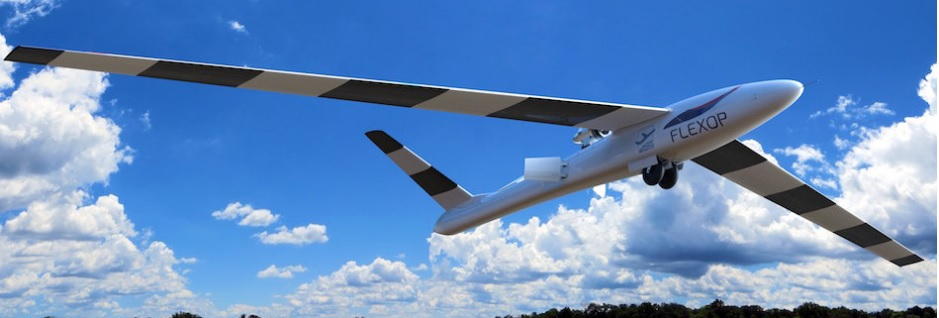
\includegraphics[width=1\linewidth]{figs/ac.jpg}
	\caption{\textbf{FLEXOP flutter demonstrator.}}
	\label{fig:ac}
\end{wrapfigure}
The proposed control system features two main parts, the baseline flight control system to navigate the aircraft fully autonomously around the predefined flight test track and the active flutter control algorithms to stabilize the aircraft's flutter modes thereby extending its operational range.
The architecture of the presented baseline controller to augment the rigid body motion features a classical cascaded flight controller architecture \cite{brock11,Stevens15,Theis18cep} with well proven feedback loops of proportional-integral-derivative (PID) controllers together with damping augmentation. These control loops provide capabilities for augmented pilot-in-the-loop flights  as well as for autonomous flights.  A major task during the design of active flutter suppression algorithms is the adequate fusion of the numerous available measurements on the wings and the different control inputs. This is commonly done in a  pre-processing step by the control engineer before deriving the control algorithm. 
In Section \ref{sec:blend} of this article, a new systematic  approach to analytically blend the available inputs and outputs to isolate the aeroelastic modes to be stabilized is presented. This enables a simple control design for each individual mode, using parametrized single-input single-output (SISO) controllers of a predefined structure.

By defining the structure of the controllers in advance, the design of the flutter suppression controller as well as the baseline controller reduces the selection of adequate control gains. For this selection a model based approach using robust control techniques is proposed in Section \ref{sec:opt}. Two generic control design problems are defined:  the first problem defines a multi-model, multi-objective optimization for deriving a controller which is robust against parameter variations. The second design is posed as parametric multi-objective problem for designing gain-scheduled controllers. Both problems are solved using non-smooth optimization based on robust control algorithms \cite{Apkarian06}.  In the case of the gain-scheduled controller, this approach enables the direct determination of the controller parameters over the entire flight envelope in a single design step, i.e., avoiding the classically applied point-wise design. 
The presented tool chain for the controller design is applied to the FLEXOP flutter demonstrator in Section \ref{sec:appl}.
A detailed overview of the baseline controller functionality and the employed loops and design criteria is provided. Further, the application of the proposed blending vector design and parameter tuning to derive the flutter suppression controller is discussed, providing valuable insight to the reader on how such algorithms are developed.
The designed flight control system of the FLEXOP flutter demonstrator is verified in an extensive verification campaign and its results are reported in Section \ref{sec:verif}. For the verification campaign a high fidelity, non-linear simulator of the closed-loop aircraft \cite{Wuestenhagen18,Meddaikar19}, including structural and aerodynamic  effects as well as detailed actuator, sensor and engine models, is available.
The verification includes wind scenarios to test the disturbance attenuation, acceleration scenarios to verify the stabilization capabilities of the active flutter control algorithm, and  flights along the predefined flight test pattern on which the real flight tests will be performed.

\section{$\mathcal{H}_{2}$-Optimal Input and Output Blending}\label{sec:blend}
In this section the theoretical background to optimally blend  inputs and outputs of a system is provided. The approach blends the inputs and outputs in a way, that the controllability and observability of the mode to be controlled is maximized in terms of the $\mathcal{H}_{2}$-norm. 
For aeroelastic control problems, this approach is especially applicable since no model order reduction of the typically high dimensional aeroelastic model is required. Furthermore, a high number of sensors, e.g. strain or acceleration measurements, are available and need to be fused accordingly within the control algorithm. 


\subsection{Modal Control of Linear Time-Invariant Systems}
\label{sec:description}
A  linear time-invariant \ac{LTI} system with $n_u$ inputs, $n_y$ outputs and $n_x$ states which is physically realizable is described by the transfer function matrix
%
\begin{align}
\label{eq:tfm}
\aemat{G}{}(s)=
\aemat{C}{}\left(s\aemat{I}{}-\aemat{A}{}\right)^{-1} \aemat{B}{} + \aemat{D}{},
\end{align}
where
%
$
\aemat{A}{} \in \mathbb{R}^{n_x \times n_x},
\aemat{B}{} \in \mathbb{R}^{n_x \times n_u},
\aemat{C}{} \in \mathbb{R}^{n_y \times n_x},
\aemat{D}{} \in \mathbb{R}^{n_y \times n_u}
$
%
and $s$ denotes the Laplace variable.
%
Assuming that $\aemat{A}{}$ is diagonalizable, a modal decomposition of $\aemat{G}{}(s)$ is possible such that
%
\begin{align*}
\aemat{G}{}(s)=\sum^{n_m}_{m=1} \aemat{M}{m}(s) + \aemat{D}{},
\end{align*}
%
where the individual modes $m=1,...,n_m$ are given as
%
\begin{align}
\label{eq:mode}
\aemat{M}{m}(s)=
\begin{cases}
\dfrac{\aemat{R}{m}}{s- \aesym{p}{m}} &
\text{if } \Im{(p_m)}=0 \\[2ex]
\dfrac{\aemat{R}{m}}{s- \aesym{p}{m}} + 
\dfrac{\aematb{R}{m}}{s-\aesymb{p}{m}} &
\text{otherwise.}
\end{cases}
\end{align}
%
According to (\ref{eq:mode}), a mode $m$ is either described by a single real pole $p_m$ with an imaginary part $\Im{(p_m)}=0$  or a conjugate complex pole pair $p_m$ and $\aesymb{p}{m}$. 
Hence, the number of modes $n_m$ does not necessarily equal the number of states $n_x$, i.e. $n_m \leq n_x$.
Each pole $p_m$ is associated with a residue 
$\aemat{R}{m}$,
where the residues of a conjugate complex pole pair are also conjugate complex.

In general, a mode $m$ is considered to be asymptotically stable if $\Re{(p_m)}<0$ and unstable if $\Re{(p_m)}>0$. In case $\Re{(p_m)}=0$, the mode is considered to be undamped, which also includes a pole in the origin. 
Furthermore, the natural frequency of a mode is given as
$\omega_{\text{n},m} = |p_m| $
and for $\omega_{\text{n},m} \neq 0$, the corresponding relative damping is
$\zeta_m = -\Re{(p_m)} / \omega_{\text{n},m}$. 
Note that for a conjugate complex pole pair, the corresponding real parts $\Re{(p_m)}=\Re{(\aesymb{p}{m})}$ and magnitudes $|p_m|=|\aesymb{p}{m}|$ are equal. For more information on modal decomposition and the properties of individual modes see, for instance, \cite{Skoge_05}.


The task of controlling a single mode $\aemat{M}{j}(s) \in \{\aemat{M}{m}(s)\}$ of a high order dynamic system is challenging when the number of control inputs or measurement outputs is increased.
To reduce the complexity of the control problem, it is proposed to weight and sum the measurement signals such that the resulting virtual measurement output $v_{y,j}$ represents the response of the mode to be controlled. Similarly, it is proposed to generate a virtual control input $v_{u,j}$ which is distributed to available control inputs such that the target mode are individually controlled.
In other words, the mode to be controlled is isolated by blending inputs and outputs. The corresponding input and output blending vectors $\aevec{k}{u,j} \in \mathbb{R}^{n_u}$ and $\aevec{k}{y,j} \in \mathbb{R}^{n_y}$ depend on the shape of the targeted mode and are seen as directional filters.
This implies a high robustness against frequency variations as the blending vectors are independent of the mode's natural frequency. 
Blending the inputs and outputs as proposed, a simple \ac{SISO} controller $c_{j}(s)$ is designed to control the isolated mode. Hence, the \ac{MIMO} control design problem becomes a \ac{SISO} one with the challenge to find adequate blending vectors.

In Figure \ref{fig:clm}, the resulting feedback interconnection is depicted, where the modes $j=1,..,n_j$ are subject to be controlled. 
Summarizing the input and output blending vectors in $K_u=[ \aevec{k}{u,1}~\cdots~\aevec{k}{u,n_j}]$
and 
$\aemat{K}{y}=[\aevec{k}{y,1}~\cdots~\aevec{k}{y,n_j} ]$,
the overall controller is
\begin{align*}
\aemat{K}{}(s)=\aemat{K}{u} \aemat{C}{}(s) \aemat{K}{y}^T,
\end{align*}
where the \ac{SISO} controllers are collected on the diagonal of
$\aemat{C}{}(s)=\diag{\left( \aesym{c}{1}(s), \cdots , \aesym{c}{n_j}(s) \right)}$.

\begin{figure}[!htbp]
	\centering
	%{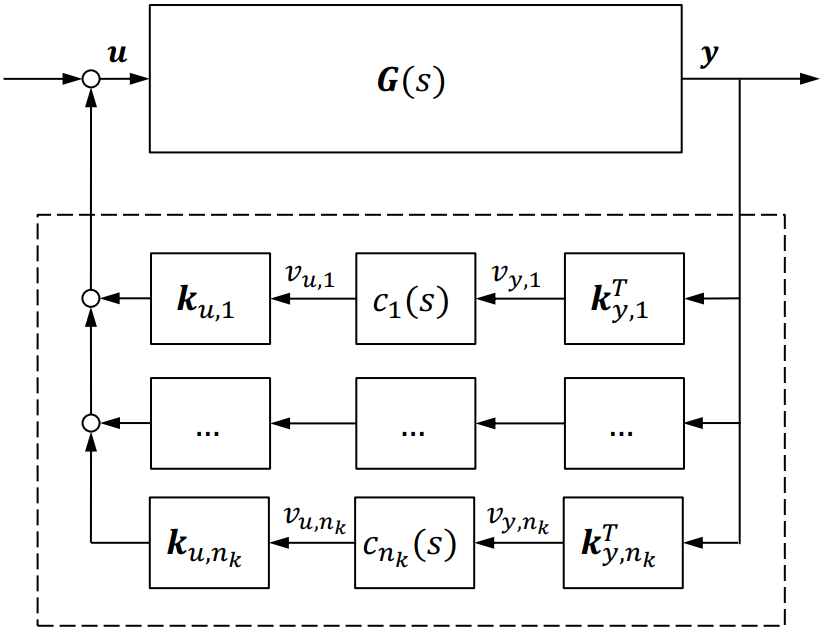
\includegraphics[width=.5\textwidth]{figs/rpdImg.png}}
	{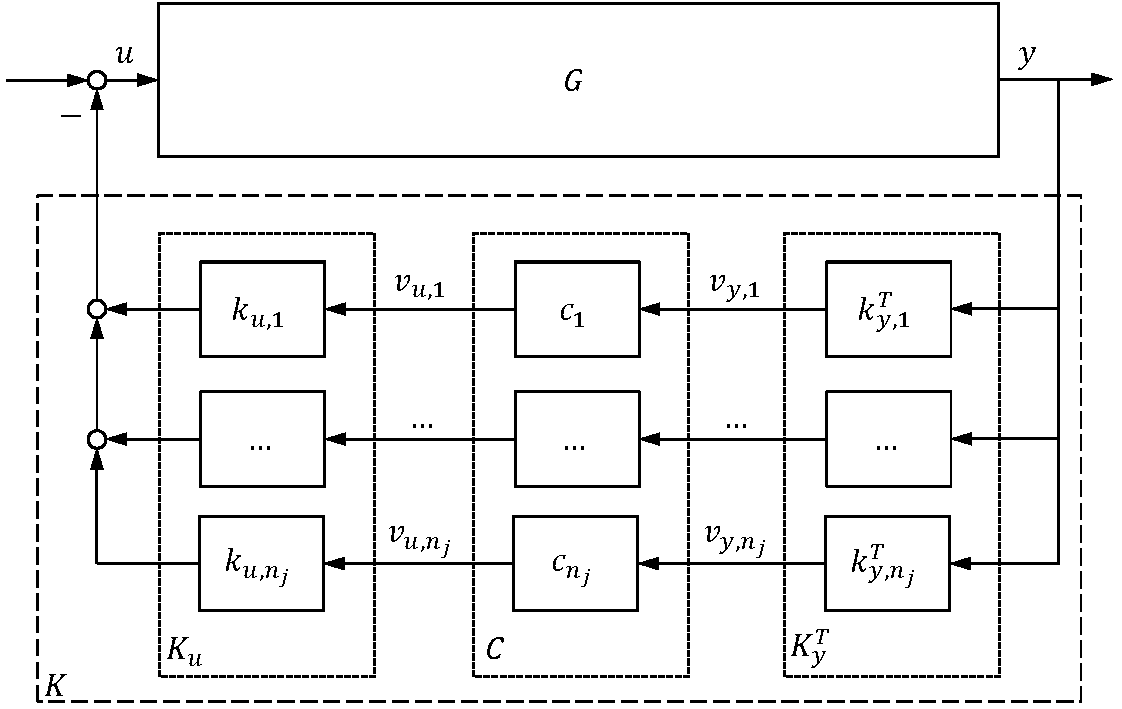
\includegraphics[width=.8\textwidth]{figs/strct.pdf}}
	\caption{Closed-loop interconnection of plant 
		$G$ with flutter suppression controller $K$, output blending matrix $K_y$, input blending matrix $K_u$, and controller $C$.}
	\label{fig:clm}
\end{figure}





%
% 
%%%%%%%%%%%%%%%%%%%%%%%%%%%%%%%%%%%%%%%%%%%%%%%%%%%%%%%%%%%%%%%%%%%%%%%%%%%%%%%%
\subsection{$\mathcal{H}_2$-Optimal Blending Vector Design}
\label{sec:contrObs}


The goal addressed herein is to find blending vectors which yield a maximum controllability and observability of the mode to be controlled in terms of the $\mathcal{H}_2$-norm.
This requires a joint design of the input and output blending vectors as controllability and observability cannot be regarded independent of each other.
%Furthermore, a sufficient mode decoupling needs to be considered in order to enable the proposed \ac{SISO} controller design.
Furthermore, the proposed method is extended to undamped and unstable modes, for which the $\mathcal{H}_2$-norm becomes infinite by definition.


In this article, the combined controllability and observability of an asymptotically stable mode $M(s) \in \{ M_j (s) \}$ is quantified in terms of the $\mathcal{H}_2$-norm. 
%The $\mathcal{H}_2$ norm perfectly captures the fact that additional control inputs or measurement outputs can only increase or at least preserve the controllability and observability of an individual mode.
Hence, the goal is to stay as close as possible to the original controllability and observability of the targeted mode when blending inputs and outputs with real-valued unit vectors $k_u$ and $k_y$, respectively.
This gives rise to quantify the loss of controllability and observability via the efficiency factor
%
\begin{align}
\label{eq:eta}
\eta=\frac{\Hnorm{ \aevec{k}{y}^T \aemat{M}{}(s) \aevec{k}{u} }{2}}
{\Hnorm{ \aemat{M}{}(s)}{2}},
\end{align}
%
where $\eta \in [0 ~ 1]$ for $\aemat{M}{}(s)$ being fully controllable and observable. Based on that, a pair of input and output blending vectors is considered as $\mathcal{H}_2$-optimal when the efficiency factor $\eta$ is maximized. The resulting optimization problem are formulated as
%
\begin{align}
\label{eq:opt}
\begin{array}{lll}
%\begin{split}
\underset{\aevec{k}{u} \in \mathbb{R}^{n_u},\aevec{k}{y} \in \mathbb{R}^{n_y}}{\mathrm{maximize \quad \quad}}
& &
\Hnorm{ \aevec{k}{y}^T \aemat{M}{}(s) \aevec{k}{u} }{2}
\\
\text{subject to}
& &
\norm{ \aevec{k}{u} }{2} = 1
\\
& &
\norm{ \aevec{k}{y} }{2} = 1.
%\end{split}
\end{array}
\end{align}
%
To efficiently solve the nonlinear optimization problem \eqref{eq:opt}, the findings in \cite{Pusch2018, Pusch18a} are applied to the objective function \eqref{eq:opt} giving
%
\begin{align}
\label{eq:applyH2norm}
\Hnorm{ \aevec{k}{y}^T \aemat{M}{}(s) \aevec{k}{u}  }{2}
&=
|\aevec{k}{y}^T \aemat{M}{}(j\omega_{\text{n}}) \aevec{k}{u}|
\sqrt{\omega_{\textup{n}} \zeta},
\end{align}
%
where the term $\sqrt{ \zeta \omega_{\text{n}}}$ is actually independent of the blending vectors. Hence, the original problem of maximizing the $\mathcal{H}_2$-norm is turned into a problem of maximizing the magnitude of the complex scalar $\aevec{k}{y}^T \aemat{M}{}(j\omega_{\text{n}}) \aevec{k}{u}$. 
Computing this magnitude according to \cite{Pusch18a} and factoring the real-valued blending vectors $\aevec{k}{y}$ and $\aevec{k}{u}$, results in
%
\begin{align}
\label{eq:outfac}
\begin{split}
|\aevec{k}{y}^T \aemat{M}{}(j\omega_{\text{n}}) \aevec{k}{u}|
%&=
%\max_{\phi} 
%\big(
%\aevec{k}{y}^T 
%%\underbrace{
%\big( 
%\Re{(\aemat{M}{}(j\omega_{\text{n}}))} \cos \phi + 
%\Im{(\aemat{M}{}(j\omega_{\text{n}}))} \sin \phi 
%\big)
%%}_{\aemat{F}{}(\phi)}
%\aevec{k}{u}
%\big)
%\\
&=
\max_{\phi} 
\big(
\aevec{k}{y}^T  \aemat{F}{}(\phi) \aevec{k}{u} 
\big),
\end{split}
\end{align}
%
where $\aemat{F}{}(\phi) : \mathbb{R} \rightarrow \mathbb{R}^{n_y \times n_u}$ is defined as
%
\begin{align}
\label{eq:F}
\aemat{F}{}(\phi)=
\Re{(\aemat{M}{}(j\omega_{\text{n}}))} \cos \phi + 
\Im{(\aemat{M}{}(j\omega_{\text{n}}))} \sin \phi .
\end{align}
%
Recalling that the actual goal is to find a maximum of (\ref{eq:outfac}) gives
%
\begin{align}
\begin{split}
\label{eq:maxmax}
\max_{\aevec{k}{u},\aevec{k}{y}} 
\left|  \aevec{k}{y}^T \aemat{M}{}(j\omega_{\text{n}}) \aevec{k}{u} \right|
&=
\max_{\aevec{k}{u},\aevec{k}{y}} \max_{\phi}
\big( 
\aevec{k}{y}^T  \aemat{F}{}(\phi) \aevec{k}{u} 
\big)
\\
&=
\max_{\phi} \max_{\aevec{k}{u},\aevec{k}{y}} 
\big( 
\aevec{k}{y}^T  \aemat{F}{}(\phi) \aevec{k}{u} 
\big).
\end{split}
\end{align}
% 
In (\ref{eq:maxmax}), the term
%
\begin{align}
\label{eq:sigmaMax}
\max_{\aevec{k}{u},\aevec{k}{y}} 
\left( 
\aevec{k}{y}^T  \aemat{F}{}(\phi) \aevec{k}{u} 
\right)
=
\norm{\aemat{F}{}(\phi)}{2}
=
\sigma_{\text{max}}
\end{align}
%
can be directly computed for a given value of $\phi$ by applying a \ac{SVD} on
%
\begin{align}
\label{eq:svd}
\aemat{F}{}(\phi)
=
\aemat{U}{} \aemat{\Sigma}{} \aemat{V}{}^T
=
\begin{bmatrix}
\aevec{k}{y,\text{max}} & \bullet 
\end{bmatrix}
\begin{bmatrix} 
\aesym{\sigma}{\text{max}} & \aemat{0}{} \\ \aemat{0}{} & \bullet 
\end{bmatrix}
\begin{bmatrix}
\aemat{k}{u,\text{max}} & \bullet
\end{bmatrix}^T,
\end{align}
%
where the placeholder $\bullet$ denotes a matrix of adequate size.
In (\ref{eq:svd}), both
$\aemat{U}{} \in \mathbb{R}^{n_y \times n_y}$ and 
$\aemat{V}{} \in \mathbb{R}^{n_u \times n_u}$ are
orthogonal matrices which are real-valued as $\aemat{F}{}(\phi)$ is also real-valued.
Furthermore, $\aemat{\Sigma}{} \in \mathbb{R}^{n_y \times n_u}$ is a rectangular diagonal matrix with the singular values of $\aemat{F}{}(\phi)$ in descending order on its diagonal.
Selecting only the largest singular value $\sigma_{\text{max}} \in \mathbb{R}_{\geq 0}$, the corresponding input and output singular vectors $\aevec{k}{u,\text{max}} \in \mathbb{R}^{n_u}$ and $\aevec{k}{y,\text{max}} \in \mathbb{R}^{n_y}$ directly yield the input and output blending vectors which solve (\ref{eq:sigmaMax}) for a given value of $\phi$.

Finally, inserting (\ref{eq:sigmaMax}) into (\ref{eq:maxmax}), an equivalent formulation of the optimization problem \eqref{eq:opt} is given as
%
\begin{align}
\label{eq:reform}
\max_{\aevec{k}{u},\aevec{k}{y}} 
\Hnorm{ \aevec{k}{y}^T \aemat{M}{}(s) \aevec{k}{u} }{2}
\Leftrightarrow
\max_{\phi} \norm{\aemat{F}{}(\phi)}{2},
\end{align}
%
where the optimization variables
$\aevec{k}{u} \in \mathbb{R}^{n_u}$ and 
$\aevec{k}{y} \in \mathbb{R}^{n_y}$ are constrained by
$\norm{\aevec{k}{u}}{2}=1$ and $\norm{\aevec{k}{y}}{2}=1$
while 
$\phi \in \mathbb{R}$ is unconstrained.
Solving $\max_{\phi} \norm{\aemat{F}{}(\phi)}{2}$ yields an optimal phase angle $\phi^*$ for which the $\mathcal{H}_2$-optimal blending vectors are directly determined according to (\ref{eq:svd}).
Hence, the number of optimization variables is reduced from $n_u+n_y$ to a single one, or, in other words, the  difficulty of finding a solution of (\ref{eq:opt}) becomes independent of the actual number of inputs and outputs.
Finally, the optimization problem (\ref{eq:opt}) has been transformed to the numerically tractable problem (\ref{eq:reform}). The latter is easily solved using readily available numerical software tools, further discussed and described in \cite{Pusch18a}. With the proposed transformations, the  computational demands of the design method are low and the optimized blending vectors are designed within fractions of a second even for complex, high order models.

In case the mode $M(s)$ is unstable, the corresponding $\mathcal{H}_2$-norm becomes infinite and the optimization problem \eqref{eq:opt} cannot be solved. Considering the definition of the $\mathcal{H}_2$-norm for asymptotically stable systems \cite{Skoge_05}, it becomes maximum iff the integral over the (squared) magnitude of the frequency response becomes a maximum. For an unstable mode, this integral is also computed by exploiting the fact that  the magnitude is not affected when mirroring the unstable pole(s) across the imaginary axis. As a result, an asymptotically stable system is obtained for which the $\mathcal{H}_2$-norm can easily be computed. 
Based on that, it is proposed to design the blending vectors of an unstable mode by first mirroring the underlying poles across the imaginary axis and then applying the algorithm described above. Note that  to preserve the magnitude of the frequency response when mirroring a pole, the zeros of each individual transfer channel need to be preserved which typically affects the corresponding residue(s).


\section{Optimization-Based Control Design}\label{sec:opt}
The controller structures of the baseline controller are defined based on classical flight-mechanical considerations. The blending vectors in the active flutter control algorithm allow defining a generic, parametrized SISO controller structure to control the flutter modes. Thus, for both design tasks only the actual gains have to be selected. 
These controller gains are derived by solving one of the two  robust control design problems specified herein. The presented  model-based gain optimizations pose non-convex design problems which are solved  using MATLAB's \texttt{systune} routine based on non-smooth optimization techniques \cite{Apkarian06}.
%The software tools allow an intuitive definition of optimization criteria  in the frequency domain (e.g., bandwidth) and in the time domain (e.g., rise time)  as either minimization criteria (soft constraint) or as minimization constraint (hard criteria). 
The software tools allow an intuitive definition of tuning requirements in the frequency domain (e.g., bandwidth) and in the time domain (e.g., rise time)  as either minimization criteria (soft requirements) or as inequality constraint (hard requirements).

For the model based approach, a low order, Linear Parameter-Varying (LPV) model of the FLEXOP demonstrator  has been derived in \cite{luspay18, Luspay18a} via linearization and advanced model order reduction techniques. It serves as basis for the design herein.
The order reduction of the full aeroservoelastic model described in \cite{Wuestenhagen18} was performed to facilitate the optimization-based control design as the full aeroservoelastic model includes modes at frequencies  far beyond the targeted flutter frequencies. The high order model is the result from detailed structural and aerodynamic computations required during the aircraft design process and is not well suited for the actual control design. The derived LPV model of the form
\begin{equation}\label{eq:model0}
G(\rho(t)): \,
\begin{array}{rcl}
\dot x(t) &=& A(\rho(t)) x(t) + B  (\rho(t)) u(t) \\
y(t) &=& C(\rho(t)) x(t) + D(\rho(t)) u(t)
\end{array}
\end{equation}
has the grid based representation
\begin{equation}\label{eq:model1}
{\mathcal{G}} = \left\{ G_i \, | \, G_i = 
\left[
\begin{smallmatrix}
A_i & B_i \\ C_i & D_i
\end{smallmatrix}
\right],
\begin{smallmatrix}
A_i = A(\rho_i)& B_i = B(\rho_i)\\
C_i = C(\rho_i)& D_i = D(\rho_i)\\
\end{smallmatrix}
\right\}.
\end{equation}
In (\ref{eq:model0})  $G(\rho(t))$ is the LPV model depending on the parameter $\rho(t)$ with the state vector $x$, the input vector $u$,  the output vector $y$, and the state space matrices $A(\rho)$, $B(\rho)$, $C(\rho)$, and $D(\rho)$. In (\ref{eq:model1})  $\mathcal{G}$ defines the set of $i=1,\dots,n_i$ linear time invariant models on the $n_i$ grid points. Thus, the model $G(\rho(t))$ is evaluated with the $n_i$ constant parameter values $\rho_i$, giving the LTI models $G_i$  with the space matrices $A_i$, $B_i$, $C_i$, and $D_i$.
Note that for the  LPV model of the flutter demonstrator the scheduling parameter is the indicated airspeed, i.e., $\rho(t) = V_\text{ias}(t)$, in an interval between 32\,m/s and 70\,m/s.
%The derived low order model of the aircraft dynamics has a state dimension of $n_x = 35$. Second order actuator models and first order linear sensors models are explicitly added to the design dynamics.

Depending on the variability of the aircraft dynamics to be considered for the underlying control design two control design problems to be solved are distinguished. In case of low variations in the aircraft dynamics over the aircraft velocity, the goal is to design a constant controller for the whole velocity range via a multi-model approach. Larger variations in the aircraft dynamics call for a scheduled controller design to achieve better performance. 


\subsection{Constant Controller Design}

The multi-model, multi-objective optimization problem  to derive constant gains of a predefined controller structure \cite{Apkarian14}  is stated by
% \begin{equation}\label{eq:problem1}
%\min_{K} \max_{i,j} || H_i^{(j)}(s) ||_\infty,
%\end{equation} 
\begin{eqnarray}\label{eq:problem1}
&&\min_\Lambda \max_{i,s} f_{s}^{(i)}(\Lambda) \\
&&\textnormal{s.t.} \max_{i,h} g_{h}^{(i)}(\Lambda) < 1 \nonumber \\
&& \Lambda_{\min} < \Lambda < \Lambda_{\max}, \nonumber 
\end{eqnarray}
where $f_{s}(\Lambda)$ are the $s=1,\dots,n_s$ posed soft requirements, and  $g_{h}(\Lambda)$ are the  $h=1,\dots,n_h$ hard requirements. The upper index $(i)$ indicates that the requirements are evaluated for all  $i= 1,\dots, n_i$ models.
The free controller gains $k_l$ to be optimized, with $l=1,\dots,n_l$,  are staked in the vector $\Lambda$ and tuned over all models and are limited by the upper and lower bounds $\Lambda_{\min}$ and $\Lambda_{\max}$. The software normalizes the soft and hard requirements and applies non-smooth optimization techniques to solve the corresponding multi-objective problem  \cite{Apkarian06}.



\subsection{Scheduled Controller Design}

The scheduled controller design problem \cite{Apkarian15} is similar to the one presented in (\ref{eq:problem1}). The main difference is that the controller gains in $K$ depend on the scheduling variables  described in the vector $\pi$. This vector belongs to the bounded region  $\Pi \in \mathcal{P}$, where $\mathcal{P}$ is the $n_p$-dimensional parameter space. The design problem is defined by
\begin{eqnarray}\label{eq:problem2}
&&\min_{\Lambda(\pi)} \max_{i,s} f_{s}^{(i)}(\Lambda(\pi)) \\
&&\textnormal{s.t.} \max_{i,h} g_{h}^{(i)}(\Lambda(\pi)) < 1 \nonumber \\
&& \Lambda_{\min} < \Lambda(\pi) < \Lambda_{\max}. \nonumber 
\end{eqnarray}
To avoid the necessity to optimize over the multi-dimensional function space $\Lambda(\pi)$, the gains in $\Lambda(\pi)$ are restricted to polynomial basis functions of the parameters in $\pi$. For example, the $l^{\text{th}}$ element of the vector $\Lambda(\pi)$ is described by
\begin{equation}\label{eq:basisf}
k_l = z_{0,l} + z_{1,l} \pi + \dots + z_{n_q,l} \pi^{\circ n_q},
\end{equation}
where $n_q$ defines the  polynomial order of the basis function. The vectors $z_{q,l}$ with $q = 1,\dots,n_q$ and $l = 1,\dots, n_l$, are constant and have the size $1 \times n_p$. The notation $\circ$ is used to indicate that the exponent is used on each element of the parameter vector $\pi$. For the control designs herein the indicated airspeed is the only  scheduling parameter of the controller, i.e., $\pi = V_{\text{ias}}$ and $n_p = 1$. Also, the scheduling parameter of the controller is equal to the  parameter of the underlying LPV design model described in (\ref{eq:model1}), i.e., $\rho = \pi = V_{\text{ias}}$. 


\subsection{Design Requirements}
The soft and hard design constraints $f$ and $g$ in (\ref{eq:problem1}) and (\ref{eq:problem2}), respectively,  are defined using classical control objectives in the frequency and time domain. This includes desired bandwidth, robustness margins, overshoot, tracking error, rise time, maximum loop gains, and desired loop shapes.
Another possibility used in this article is to provide a \textit{reference model} and use the error between this reference model and the resulting dynamics as criteria to be minimized in either (\ref{eq:problem1}) or (\ref{eq:problem2}). Such a model matching setup provides an elegant way to achieve the desired dynamics
over the whole parameter range.


\section{Application to the FLEXOP Demonstrator}\label{sec:appl}
The presented approaches to optimally blend input and outputs in Section \ref{sec:blend} and the optimization to determine the controller parameters in Section \ref{sec:opt} are applied to the FLEXOP aircraft. 
The single-engined FLEXOP flutter demonstrator features a wing span of 7\,m and is illustrated in Figure \ref{fig:ac}. The takeoff weight is typically 55\,kg but can be increased by up to 11\,kg of ballast.
Two wing-sets are designed and manufactured for the aircraft. The first one features a rigid structure with a flutter speed far beyond the operational aircraft velocity. This wing-set is mainly used for basic flight testing and rigid model verification. The second wing-set, which is considered in the models in this article, is flexible and has two main flutter modes within the operational velocity range.

The  rigid body motion of this aircraft is described by a standard nonlinear six-degrees-of-freedom flight mechanics model (e.g. \cite{McRuer73}) in terms of translational velocities $u$, $v$, $w$ and angular velocities $p$ (roll), $q$ (pitch), $r$ (yaw) in the body-fixed frame.  Orientation in the earth-fixed reference frame is described in terms of Euler angles $\Phi$ (bank), $\Theta$ (pitch), and $\Psi$  (heading). The angles between body-fixed frame and wind axes are angle of attack $\alpha$ and side-slip angle $\beta$. The flight path is described with respect to earth by the path angle $\gamma$ and the course angle $\chi$. To describe the flutter phenomena, the structural dynamics from a reduced finite element model are coupled with aerodynamics derived via the doublet lattice method. This coupling to derive the aeroelastic model is achieved via splining.
For the flexible wing-set the first flutter mode (symmetric), becomes unstable at around 52\,m/s with 8\,Hz, while the second one (asymmetric) mode, follows at 54.5\,m/s with 7.3\,Hz \cite{Meddaikar19,Iannelli18}. A detailed description of the aircraft modeling and its analysis is also provided in \cite{Wuestenhagen18,Rozov17}.

As control inputs the aircraft features four ruddervators on the aircraft's V-tail, two on the left ($\delta_{rv,l1}$, $\delta_{rv,l2}$) and two on the right side ($\delta_{rv,r1}$, $\delta_{rv,r2}$) as illustrated in Figure \ref{fig:ac_u}.  These ruddervators combine the functionalities of classical rudders and elevators. The symmetric deflections of the ruddervator correspond to classical elevator deflections, while asymmetric deflections exhibit rudder deflections. Additionally, the aircraft has four pairs of ailerons. The most outer pair ($\delta_{a,l1}$, $\delta_{a,r1}$) is used for flutter control while the most inner pair ($\delta_{a,l4}$, $\delta_{a,r4}$) is used as high lift devices during takeoff and landing. The inner two pairs ($\delta_{a,l2}$, $\delta_{a,r2}$, $\delta_{a,l3}$, $\delta_{a,r3}$) are used in the baseline control law to control the aircraft's roll motion. This rigorous dedication of each aileron pair to a single task is taken to simplify the control design tasks and avoid superposition of baseline and flutter control signals in the actuator commands during aircraft operation. The latter could result in actuator saturation which needs to be absolutely avoided to ensure stabilization of the flutter modes.

 \begin{wrapfigure}{r}{0.55\textwidth}
	\centering
	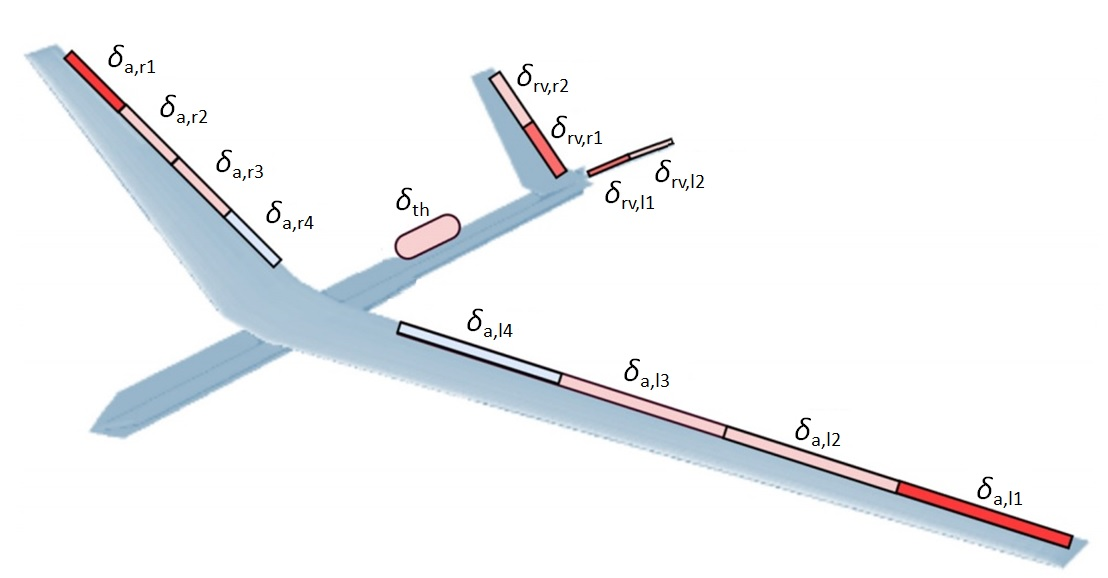
\includegraphics[width=1\linewidth]{figs/ac_u.jpg}
	\caption{\textbf{Control surface configuration.}}
	\label{fig:ac_u}
\end{wrapfigure}
 The actuators to steer the control surfaces are modeled as second order systems with rate and position limits to realistically reflect the actuator behavior. 
 These  models have been obtained through frequency-based system identification and data gathered on the various servos. The sensors of the aircraft are modeled as first order linear models including time delays.
 The aircraft is equipped with a 300\,N jet engine \cite{Sendner17}, located on the fuselage dorsal surface.  A high fidelity, non-linear simulation model of the engine is available. Consequently, a simplified, control-oriented model has been developed and is considered in the controller design tasks. It features a dominant time delay of $1\,$s, a non-linear mapping from the engine's revolution-speed  to thrust  (and versa), and a rather slow second-order dynamic. In addition, a velocity dependent saturation limit is considered. It describes how the available thrust decreases with increased inflow speeds. 








\subsection{Baseline Controller}
Three different modes to control the aircraft are considered in the flight control system. These modes facilitate a stepwise augmentation of the aircraft during the flight test campaign:

\begin{itemize}
	\item[(i)] \textbf{Direct Mode}: The direct mode allows the pilot on the ground to bypass the flight control system. The only part active in the flight control computer is the mapping from the received remote-control signals to the commanded surface deflections. The pilot controls the pitch, roll and yaw axis directly via the aircraft's control surface deflections and its velocity via the thrust setting. 
	
	\item[(ii)] \textbf{Augmented Mode}: The augmented mode switches on basic augmentation for the pilot \cite{Weiser2018}. Instead of directly controlling the surfaces the pilot inputs pitch- and roll-attitude commands. The side-slip angle is automatically regulated to zero, reducing the pilots need to control the yaw axis separately. Velocity control remains in direct control, i.e., the pilot controls the velocity via the thrust setting.
	
	\item[(iii)] \textbf{Autopilot Mode}: In this mode the pilot  fully delegates the aircraft control to the flight control system. Altitude, course angle, velocity and side-slip angle are automatically controlled. To fly along the defined test pattern, reference commands based on the aircraft position are generated in a navigation module.
\end{itemize}

The inner loops of the control system in roll, pitch and yaw provide the basis for the operational model (ii) and (iii). Mode (iii) is the core element of the autopilot  adding the outer loops for course angle, altitude and speed control (autothrottle) as illustrated in Figure \ref{fig:arch}. Thus, a series of cascaded control loops is used to facilitate the control design task. As the cross-coupling between longitudinal and lateral axis is negligible, longitudinal and lateral control design is separated.  Thrust commands $\delta_{th}$ which are transferred to an engine revolution command $\delta_{\omega}$ via a nonlinear mapping and the  elevator $\delta_e$ are the available actuators for longitudinal control.
The available bandwidths for throttle and elevator differ considerably such that a combined control design does not promise any advantages. Thus, the reference $V_{\text{ref}}$ for the indicated airspeed $V_{\text{ias}}$ is controlled solely by the use of the throttle command  $\delta_{th}$. The elevator command  $\delta_{e}$ is used to control the attitude in the inner loop and the vertical position of the aircraft in the outer loop. The pitch-attitude controller in the most inner feedback loop tracks the pitch-attitude ($\Theta$), attenuates wind disturbances, and improves short period damping with the pitch rate ($q$) measurement as an auxiliary feedback signal. The cascaded outer loop establishes control of the altitude ($H$). Both controllers are scheduled with velocity ($V_{\text{ias}}$), indicated by $\nearrow$ in Figure \ref{fig:arch}, to achieve optimal performance over the required velocity range.
\begin{figure}[!bhtp]	
	\centering
	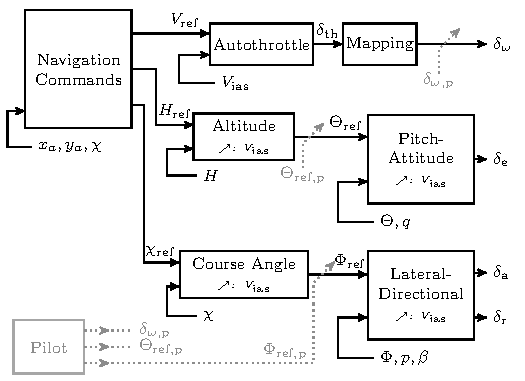
\includegraphics[width=0.7\linewidth]{figs/architecture.pdf}
	\caption{\textbf{Control architecture for fully automated flight (mode (iii)), and augmented flight (mode (ii)), indicated in gray.}}
	\label{fig:arch}
\end{figure}

Lateral-directional control generates aileron ($\delta_a$) and rudder commands ($\delta_r$). 
The lateral-directional control problem is necessarily multivariable and requires the coordinated use of aileron command $\delta_{a}$ and rudder command $\delta_{r}$. The most inner loop features roll-attitude ($\Phi$) tracking, roll-damping augmentation via the roll rate ($p$), and coordinated turn capabilities, i.e. turns without side-slip, via feedback of the side-slip angle ($\beta$). The outer loop establishes control of the course angle ($\chi$). Again, all controllers are scheduled with velocity to increase performance over the velocity range. Within the fully automated flight mode (iii) the reference signals for the velocity ($V_\text{ref}$), altitude ($H_\text{ref}$), and course angle ($\chi_\text{ref}$) are provided by a dedicated navigation algorithm. It uses the GPS longitudinal and lateral position of the aircraft ($x_a$ and $y_a$) as well as the current course angle  ($\chi$) to provide the commands.  More details on the algorithm are found in \cite{Ossmann19a}.


The control loops use scheduled elements of proportional-integral-derivative (PID) controller structures with additional roll-offs in the inner loops to ensure that no aeroelastic mode is excited by the baseline controller. Scheduling with indicated airspeed $V_{\text{ias}}$ is used to ensure an adequate performance over the velocity range from 32\,m/s to 70\,m/s. For the scheduling a first or second order polynomial in  $V_{\text{ias}}$ following (\ref{eq:basisf}) is applied. As an example, the proportional gain $k_p = z_0 + z_1 V_{\text{ias}} + z_2 V^2_{\text{ias}}$ depends quadratically on  $V_{\text{ias}}$ with the free parameters $z_0$, $z_1$, and $z_2$. These free parameters are directly included in the optimization problem (\ref{eq:problem2}). A comprehensive summary of the used controller structures for each cascaded  loop is provided in Table \ref{tab:con}, including the channel description in the controller architecture and the implemented scheduling. 

\begin{table}[H]
	\caption{Summary of the control loops of the FLEXOP baseline flight control system with the inner loop functions (first part) and autopilot functions (second part).}
	\centering
	%% \tablesize{} %% You can specify the fontsize here, e.g.,  \tablesize{\footnotesize}. If commented out \small will be used.
	\begin{tabular}{lccc}
		\toprule
		\textbf{Control Loop}     &                   \textbf{Channel}                    & \textbf{Structure} & \textbf{Scheduling} \\ \midrule
		Pitch Attitude Control            &   $(\Theta_\text{ref}-\Theta) \rightarrow \delta_e$   & PI &        2$^{\text{nd}}$-order polyn. in $V_{\text{ias}}$        \\
		Pitch Damping            &               $q \rightarrow \delta_e$                & P  &        1$^{\text{st}}$-order polyn in $V_{\text{ias}}$            \\
		Roll Attitude Control &     $(\Phi_\text{ref}-\Phi) \rightarrow \delta_a$     & P  &         1$^{\text{st}}$-order polyn in $V_{\text{ias}}$               \\
		 Roll Damping &               $p \rightarrow \delta_a$                & P  &         1$^{\text{st}}$-order polyn. in $V_{\text{ias}}$               \\
		Yaw Control  &             $\beta \rightarrow \delta_r$              &PID &         2$^{\text{nd}}$-order polyn. in $V_{\text{ias}}$              \\
		 \hline
		Autothrottle              & $(V_\text{ref}-V_\text{ias}) \rightarrow \delta_{\text{th}}$ &2 DOF-PID &   none       		\\
		Altitude                  &   $(H_\text{ref}-H) \rightarrow \Theta_\text{ref}$    & PI  &      2$^{\text{nd}}$-order polyn. in $V_{\text{ias}}$                 \\
		Course Angle              & $(\chi_\text{ref}-\chi) \rightarrow \Phi_\text{ref}$  & PID &     2$^{\text{nd}}$-order polyn. in $V_{\text{ias}}$                  \\
		\bottomrule
	\end{tabular}\label{tab:con}
\end{table}

Note that these controller outputs $\delta_e$, $\delta_a$, and $\delta_r$ deffer from the actual surface inputs to ease the actual control design task. Thus, they need to be transformed to physical actuator commands via an adequate control allocation.
The FLEXOP aircraft has multiple control surfaces and features combined rudder and elevator surfaces (ruddervators) as depicted in Figure \ref{fig:ac_u}. The commands to the actuators of the two aileron pairs are determined by
\begin{equation}\label{eq:CAail}
\begin{array}{rclcr}
\delta_{a,l2} &=& \delta_{a,l3} &=&  0.5 \delta_{a} \\
\delta_{a,r2} &=& \delta_{a,r3} &=&  -0.5 \delta_{a} \\
\end{array}
\end{equation}
to generate the required differential aileron deflections for roll motion control. For the ruddervators superposition of the elevator command $\delta_e$ and the rudder command $\delta_r$ is applied by
\begin{equation}\label{eq:CAelev}
\begin{array}{rclcl}
\delta_{elev,l1} &=& \delta_{elev,l2} &=&  \delta_e + 0.5 \delta_r \\
\delta_{elev,r1} &=& \delta_{elev,r2}  &=& \delta_e - 0.5 \delta_r.
\end{array}
\end{equation}
Thus, symmetric deflections on the left and right of the ruddervators correspond to elevator commands while differential deflections establish rudder commands.



\subsubsection{Parameter Tuning}
With the baseline controller structure available, the next step is to tune the free parameters of the individual control loops. 
Following the  ideas of the model-based approach presented in Section \ref{sec:opt}, an individual  optimization problem is set up for the tuning of each control loop.  The aircraft model used for the baseline controller design has the form (\ref{eq:model0})-(\ref{eq:model1})  and represents the aircraft with the rigid wing-set.
This model is substantially less complex than the model with the flexible wing-set. However, as the rigid body modes are barely changing with the wing-set, the baseline controller is used for both wing-sets. To not interfere with the flutter controller or excite flutter modes when using the flexible wing-set, adequate roll-off filter are included in the the design. Six  optimization problems  are deified for the baseline controller design problem, which are summarized in Table \ref{tab:opt}.
Note that the proportional damping augmentations in roll and pitch are not tuned separately but included in the optimization problems of the corresponding tracking loops. For the inner loops a phase margin of at least \SI{45}{\degree} is demanded. As short period damping is relevant, a minimum of 0.6 is set as an optimization constraint. For the roll motion a fast response time of 1\,s with good tracking capabilities (steady state error of 0.1) is defined. For the coordinated turn capabilities  via the side slip angle feedback a single constraint on the disturbance rejection gain is applied.

\begin{table}[H]
	\caption{Overview of the six defined optimization problems with the number of free parameters and optimization criteria within the model based design procedure of the baseline controller.}
	\centering
	%% \tablesize{} %% You can specify the fontsize here, e.g.,  \tablesize{\footnotesize}. If commented out \small will be used.
	\begin{tabular}{lccc}
		\toprule
		\multirow{2}{*}{\textbf{Channel} } & \multirow{2}{*}{\textbf{Structure} } &    \textbf{Free }    &   \multirow{2}{*}{\textbf{Criteria} }   \\
		&                                      & \textbf{ Parameters} &                                         \\ \midrule
		Pitch Attitude Control             &                  PI                  &  \multirow{2}{*}{8}  &        Damping ration of 0.6          \\
		\,\, incl. Pitch Damping           &                  P                   &                      &         Phase margin of \SI{45}{\degree}         \\
		Roll Attitude Control              &                  P                   &  \multirow{2}{*}{4}  &   Response time of 1s, steady state   \\
		\,\, incl. Roll Damping            &                  P                   &                      & Error of 0.1, phase margin of \SI{45}{\degree} \\
		Yaw Control                        &                 PID                  &          9           &       Disturbance rejection gain        \\
		Auto-Throttle                      &              2 DOF-PID               &          5           &          Model matching error           \\
		Altitude                           &                  PI                  &          6           &           Bandwidth criterion           \\
		Course Angle                       &                 PID                  &          9           &          Response time of 5\,s          \\ \bottomrule
	\end{tabular}\label{tab:opt}
\end{table}

For the outer loops, an adequate frequency separation is commonly required within the cascade controller design.
The bandwidth of each cascaded loop is constrained by the lower-level control loops with the ultimate constraints being the servo actuator bandwidths.  While the available servo actuators on the FLEXOP aircraft provide a sufficiently high bandwidth for the inner loop designs, the inner  and outer loops need to be frequency separated from each other. Thus, the bandwidth design constrains for the outer loop are set to be five times lower than the bandwidths of their according inner loops.
Finally, the auto-throttle is a little more involved due to the complex engine dynamics. Therefore, a model matching problem using the non-linear simulator is used which aims to minimize the recorded error between the desired and achieved response in the simulation. More details on the tuning are provided in \cite{Ossmann19a}.





\subsection{Flutter Suppression Controller}
The two flutter modes mainly limiting the operational velocity range of the aircraft with the flexible wing-set are  well distinguishable by their symmetric and asymmetric mode shapes. Both modes describe a dynamic coupling of the wing bending and torsion which becomes unstable above certain airspeeds.
To individually stabilize the two flutter modes, the $\mathcal{H}_2$-optimal blending approach proposed in Section \ref{sec:blend} is applied to the FLEXOP demonstrator. In doing so, the flutter modes are decoupled which allows for a straight forward design of two dedicated SISO control loops, one for each flutter mode. 


\subsubsection{Input-Output Blending}
The measurement signals considered for flutter suppression are captured by the inertia measurement units (IMUs) located in the wings and in the center of gravity, where only vertical acceleration and pitch rate measurements are used for the controller design herein.
In Figure \ref{fig:sens}, the location of the IMUs in the wings together with the location of the ailerons, of which only the outer pair is used for flutter suppression.

\begin{figure}[!h]	
	\centering
	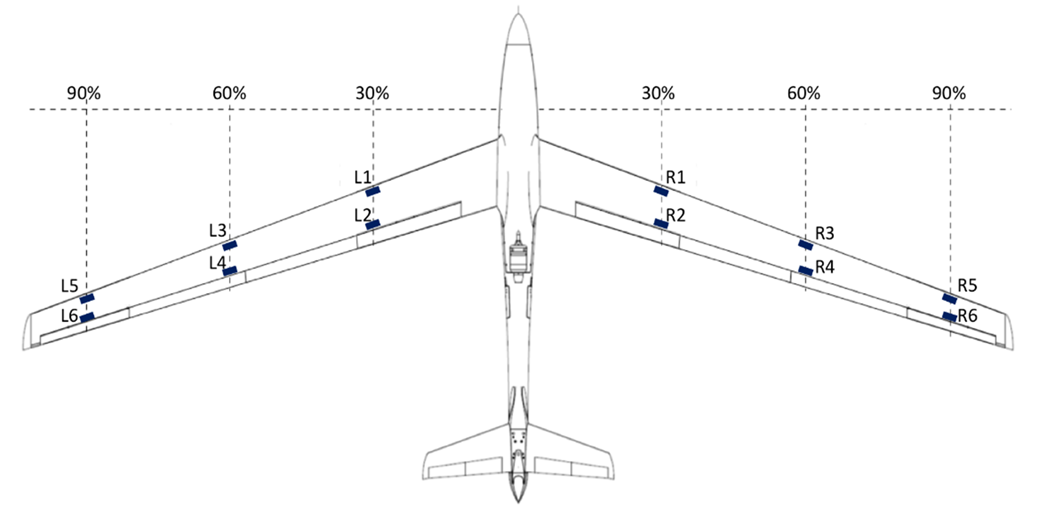
\includegraphics[width=0.75\linewidth]{figs/SensorPos}
	\caption{Locations of the IMUs installed in the wings to measure the accelerations on the wing.}
	\label{fig:sens}
\end{figure}

Before actually blending the given inputs and outputs, it is proposed to normalize the rate and acceleration measurements since they are of different units, see \cite{Pusch2018} for more details. Subsequently, the $\mathcal{H}_{2}$-optimal blending vectors associated to the first (symmetric) and second (asymmetric) flutter mode are computed according to Section \ref{sec:contrObs}. 
The obtained input and output blending vectors basically mirror the shape of the underlying modes and hence are also symmetric and asymmetric. Furthermore, sensors at the outer part of the wing are better suited to measure the corresponding flutter modes and hence are higher weighted in the output blending vector.
Since the mode shapes change only slightly within the critical airspeed range, it is sufficient to compute the blending vectors at a single airspeed $V_\text{ias}=\SI{60}{\meter\per\second}$ and hold them constant within the whole flight envelope.

\begin{figure}[h]
	\centering
	% This file was created by matlab2tikz.
%
%The latest updates can be retrieved from
%  http://www.mathworks.com/matlabcentral/fileexchange/22022-matlab2tikz-matlab2tikz
%where you can also make suggestions and rate matlab2tikz.
%

\definecolor{mycolor111}{rgb}{0.97650,0.58870,0.35690}%
\definecolor{mycolor222}{rgb}{0.71387,0.92550,0.34291}%
\definecolor{mycolor333}{rgb}{0.28636,0.81217,0.49968}%
\definecolor{mycolor444}{rgb}{0.38492,0.48677,0.96454}%
\definecolor{mycolor555}{rgb}{0.47060,0.00000,0.52160}%

\begin{tikzpicture}

\begin{axis}[%
width=2in,
height=0.90in,
at={(0in,0in)},
scale only axis,
xmode=log,
xmin=10,
xmax=1000,
xtick={10,100,1000},
xminorticks=true,
xticklabels={\empty},
xmajorgrids,
xminorgrids,
ymin=0,
ymax=2000,
ylabel={Magnitude (abs)},
title style = {yshift=-3mm, xshift=-23mm},
ymajorgrids,
axis background/.style={fill=white},
title={(a)}
]
\addplot [color=mycolor111,solid,line width=2.0pt,forget plot]
  table[row sep=crcr]{%
10	57.6767616791367\\
10.3009976241392	58.0380421661166\\
10.8196621682864	58.8490304426256\\
11.7546695882245	61.2398701164998\\
12.5557433680404	64.5862277594918\\
13.4114098521337	69.615639860744\\
14.5703894513611	78.4126242403273\\
16.1706307191245	92.5947382211094\\
18.4341641574008	113.231632212835\\
20.1401526751531	127.901053376092\\
23.042815644404	150.026343418728\\
25.6558613759614	166.634834865451\\
27.9515555151375	179.093322038782\\
29.9295741044465	188.966662421649\\
32.0475690731571	199.67555678328\\
33.6598806544425	208.725278745434\\
36.2764301920665	227.259663479294\\
38.4827382182282	249.838981193821\\
40.8232324110147	287.268756058461\\
40.8574523734901	287.973997017605\\
42.0861050838068	317.71974570065\\
43.1870528949721	354.231725550131\\
44.1700647310094	399.136312468747\\
45.0450557364151	454.571709396774\\
45.8217931097341	523.434877691059\\
46.5096868205503	609.770733295096\\
47.1176487760156	719.382414980871\\
47.6755308703812	867.851468303711\\
48.244319123928	1108.87186105027\\
48.7410118247178	1477.31453923651\\
49.1740943835313	2098.33506145319\\
49.5512221887689	3336.69649447978\\
49.8792558317113	6822.40102277457\\
50.1643095597012	20594.957169181\\
50.4509923342052	6714.45521699058\\
50.7849825381683	3224.20361961846\\
51.1744646271371	1985.04496260926\\
51.6291693461597	1363.8152511843\\
52.160710303266	995.35709812634\\
52.7830085509315	754.44306750373\\
53.5128329257108	586.789741931482\\
54.3704941823088	465.105911954953\\
55.3807456130242	374.180326338774\\
56.5739639640362	304.851136980227\\
57.9877152749462	251.231278879317\\
58.0270459285858	250.030797369271\\
59.6289606391401	210.096141345559\\
62.6810272521399	163.419764321209\\
66.8238946498117	125.918468036119\\
67.0664228610935	124.110923671601\\
71.1052505898031	95.0602695214478\\
74.3600821017626	70.4105568348754\\
76.9515922878525	56.8841333952689\\
78.8112964732364	60.6462906774607\\
80.5541950691318	73.5751110454095\\
83.1520341431373	94.9104497530289\\
86.1163005449653	111.589189902924\\
87.2758327997391	116.02246193447\\
89.0466858502046	121.598944570322\\
89.5109577595921	122.990237464616\\
90.6165531876092	126.597072646586\\
92.0046573039841	133.050663537805\\
93.2295579009055	142.375733898924\\
95.3997391736277	144.284018052502\\
95.5046127955983	143.533460344414\\
97.6558052781968	133.013489688864\\
99.4237830084284	130.352816613482\\
101.663252792542	129.325439360031\\
104.719548123187	129.111820716596\\
108.926492293883	129.423017569841\\
112.603883611701	129.878834505663\\
118.214185635544	130.676700578765\\
121.129973394955	131.086765199989\\
121.556675528574	131.14440518986\\
124.192709584534	131.478439324706\\
128.644627903386	131.90793856172\\
133.256133502232	132.051998780357\\
139.523825414426	131.371407746894\\
140.828719541478	131.035509784578\\
144.740392964472	129.424457217298\\
148.472559792791	126.738851310226\\
151.765704332168	123.23564217803\\
155.247512251315	119.086995781747\\
155.369045771852	118.962062669274\\
161.267440465789	118.335819585796\\
161.566222094188	118.57847352568\\
162.201444208283	119.134521304981\\
162.883363821577	119.768227171705\\
164.457195025507	121.229792267317\\
164.475251983872	121.245796654768\\
165.755650616518	122.297826227489\\
165.78239106313	122.31780328757\\
167.353490317413	123.323888552014\\
167.792543590899	123.54335166681\\
168.316575150768	123.769320718604\\
168.321170535624	123.771129645891\\
169.913637857899	124.221081458392\\
170.104497981348	124.252044345492\\
170.561361267404	124.307357689465\\
170.567028510081	124.307881744603\\
173.925344466185	124.18995207509\\
176.87490944622	124.017216349768\\
180.480453839771	123.037141758834\\
185.384057456218	120.837636447136\\
192.104766308166	117.178519072266\\
199.716274793248	112.783495985828\\
199.971196441826	112.637536797471\\
204.146810904938	110.29687830112\\
204.38333040899	110.16802005288\\
208.086661839592	108.22763971852\\
208.306025215212	108.118186522215\\
211.58092304842	106.58426325029\\
211.677173435431	106.542507483861\\
217.220920425551	104.598624980792\\
220.168499522175	103.948493905745\\
220.330337121264	103.913697309559\\
223.227000352444	103.02556709533\\
228.571967170029	99.9657439203928\\
231.346860714288	98.5405184688862\\
237.11353458668	96.4887815989708\\
244.955367277462	95.1012532389735\\
250.462266745758	94.9440873396891\\
256.231275043579	95.4610162465885\\
265.869404733094	96.8111182046124\\
273.37013947894	95.2021135907509\\
279.161135786301	91.9499330053935\\
285.074806934065	88.4655572642115\\
293.003698004502	83.9681769275707\\
297.365909223065	82.4981540677539\\
301.534813394068	81.970160752871\\
307.985092058193	79.698959172072\\
313.46730198484	75.0596603269828\\
321.227660286933	71.972103527441\\
326.141464392196	74.7276216332175\\
328.922237501536	77.5884063286612\\
330.728592458625	79.8339562897704\\
333.855746613122	84.3085793763754\\
336.075895165738	87.8699925997556\\
339.607567684963	94.1038443409368\\
341.844975168111	98.3851660665393\\
341.880623140984	98.4553743350487\\
347.912536478256	111.188188568402\\
348.211127781683	111.859934751871\\
353.255142605015	123.643222333586\\
357.963738522089	134.627861604519\\
358.204920299329	135.156547298016\\
362.114756919538	143.098772308483\\
366.311920163059	152.130038084115\\
366.503086953519	152.58421725303\\
371.196569742548	164.01526948714\\
371.359494188823	164.402971212052\\
374.162869510452	170.782206949526\\
376.894974666378	176.328238192358\\
377.65287926575	177.729849525773\\
383.546443709453	186.342223564485\\
383.63794969328	186.442257398425\\
388.502236075581	190.212932566854\\
391.340982995604	191.015255747074\\
391.387216680684	191.020015465295\\
392.551616963161	191.054656975872\\
402.089861208955	186.068339088796\\
403.464266173268	184.771418549056\\
410.229704106058	177.41976966772\\
411.593343699341	175.843083638095\\
417.496702635526	169.005348364131\\
419.324258860143	166.924283258951\\
423.338930367482	162.474423457791\\
423.349929340188	162.462518271405\\
425.191090311099	160.49630726743\\
426.777014399611	158.849762134397\\
430.832312666231	154.8856929821\\
430.841989361645	154.876731591949\\
437.459353615961	149.526296645288\\
437.467818790884	149.520664919389\\
443.307732730284	146.6095633265\\
443.315093831898	146.607216848025\\
448.459376346781	145.809330909733\\
448.46573592621	145.80934043057\\
453.670886800674	146.43127835935\\
453.683056855464	146.433721086465\\
459.735997346854	147.337796421155\\
459.740059538579	147.33777609104\\
466.798313399484	144.300212767166\\
466.810388183909	144.289012834911\\
471.465544906702	138.585089752772\\
473.356454026836	135.680142732258\\
473.869554962802	134.857929543226\\
474.104060586423	134.478595868885\\
483.050790073432	119.836439914483\\
495.998243018286	106.914838292182\\
510.719968446178	130.515614892451\\
522.115103582563	179.108669690131\\
533.7644858853	215.43372671618\\
543.582538071229	230.618980371447\\
551.964529985218	249.613251977019\\
560.032806267187	282.850598952433\\
563.987217626016	303.60152163087\\
567.648193157863	321.584578648354\\
582.800354723768	318.694692221624\\
594.392947479961	286.994174437233\\
598.692265847451	282.801037624453\\
599.403518559589	282.433458505508\\
607.993612458252	279.325883776109\\
616.490649652678	264.601281210336\\
626.835178161157	226.306872195113\\
639.263026440993	176.708757354346\\
654.121062779022	130.893949754849\\
665.622343531674	108.936928782504\\
681.137918754337	130.312987548339\\
702.237874598875	133.680993111405\\
715.551140750609	129.877996489325\\
731.182493956539	125.288497147729\\
749.591503768499	120.60140285575\\
771.347822710829	116.088287072304\\
797.163934652329	111.848921729026\\
822.908393852559	108.485332067094\\
834.016632081645	107.234185693109\\
864.824697488034	104.238685648627\\
903.328186396163	101.213865398725\\
925.044810495071	99.7580105489071\\
963.320358203508	97.5040224199808\\
963.87551414333	97.4737204368612\\
990.307365984352	96.0951773190429\\
990.377799888513	96.0916584010487\\
1000	95.6178384386644\\
};\label{line:v5}
\addplot [color=mycolor222,solid,line width=2.0pt,forget plot]
  table[row sep=crcr]{%
10	59.2905991260752\\
10.8647112533341	60.8945908206094\\
11.7199763499334	63.4146875394316\\
12.492344830646	66.7933610339367\\
13.4757364974108	72.7095351054903\\
14.8196295118741	83.0058000143723\\
16.6966948138279	98.9903510485192\\
18.759937781813	116.166055352034\\
21.414396738068	136.621573364234\\
23.8276132085712	153.754763679258\\
25.9716250966874	168.097353490788\\
27.9453400086146	180.958779324254\\
30.4598655161197	197.813954432349\\
32.8619929045075	216.034151046858\\
35.2081692630452	238.395929409199\\
37.3007938391128	265.574865470678\\
38.5762310433024	287.761854899622\\
39.7460063704293	313.918355086988\\
40.7851604562865	343.931846498147\\
41.7047912752435	378.188685427135\\
42.5159889322313	417.019404870796\\
43.2295195442864	460.68188165964\\
43.8556115797473	509.336630754262\\
44.4038223978497	563.015751384105\\
44.8829657616897	621.58849076152\\
45.3010843411289	684.728966296506\\
45.6654543194813	751.90074248516\\
45.9826119825077	822.452032228044\\
46.2583945260437	896.019466728897\\
46.5358310863492	982.757045581314\\
46.8590337272575	1104.31854721061\\
47.235934751883	1281.22043650513\\
47.6759730069708	1539.2415332139\\
48.1904248006978	1859.54169548512\\
48.6313030623895	1987.20984793355\\
48.792822333261	1965.83285549531\\
49.234970330241	1749.00761899823\\
49.9374087569905	1290.96838209736\\
50.7563875161934	919.206638678093\\
51.7133995840441	668.729478924185\\
52.8346123760664	501.398780755661\\
54.1521152537062	386.382051725268\\
55.7055744244887	304.908520119144\\
56.2676413150353	283.688470248637\\
59.0916788573442	212.627538171963\\
62.2938302156907	168.570535879402\\
66.6390057170239	131.90035564004\\
66.8530314003707	130.382915485392\\
69.1631010821089	114.465018379668\\
71.253761146562	99.8553982978557\\
73.0744315311267	86.4748058904031\\
76.0971245693964	66.3608273679711\\
78.452564024188	64.3191945816416\\
79.7721633464565	71.5633366181406\\
82.1304405771294	91.2765574086828\\
85.1223500664666	112.812508279125\\
87.2570296227328	122.977028638537\\
89.0278642265997	129.356752862437\\
90.5976031068399	134.965995673766\\
91.9856887935318	141.990639583528\\
93.2032229564563	151.872711641251\\
94.2893499367462	158.766369354422\\
95.3806368640722	154.016847488372\\
96.5729503981848	146.185420406327\\
98.1450140644651	141.18664668033\\
99.4237217815561	139.569999495516\\
101.042191756168	138.727093034668\\
103.249140479095	138.408094896797\\
106.277828426608	138.504974920042\\
110.469921712643	138.965046284704\\
114.566706918036	139.541153117087\\
120.092823075894	140.355760345841\\
121.370995632698	140.534863880504\\
123.589412894223	140.825398912725\\
128.618338693592	141.325736810819\\
133.851894437414	141.444557238909\\
140.904740282423	140.394457216835\\
141.21633828578	140.299890150796\\
144.694958993588	138.850785754089\\
148.492625424996	136.234859855123\\
151.97329896661	132.761124902392\\
155.502481625041	128.972121910517\\
155.535179752513	128.942689220436\\
161.568363073229	128.565398653059\\
161.911587287249	128.823771119865\\
162.040898815744	128.924768169304\\
162.87712894117	129.610440228082\\
164.453910102128	130.928040201323\\
164.472773278485	130.943165299948\\
165.751687966568	131.894245575728\\
165.76893849229	131.905900690603\\
167.351145801573	132.814229171492\\
167.663496347699	132.95366479332\\
168.310033874896	133.198913549771\\
169.911120293867	133.555775906508\\
169.916276862971	133.556361500622\\
170.550688062715	133.602081367912\\
170.564698217316	133.602515194285\\
173.833606646226	133.276861477469\\
176.830319464552	132.93857066863\\
180.530219246414	131.725154658243\\
185.562091047121	129.141161862572\\
192.459761482672	124.92687160051\\
199.730412283355	120.26994046198\\
199.967564800597	120.119647065869\\
204.16586275299	117.515728565593\\
204.387354977859	117.38222374404\\
208.110236276464	115.223494011734\\
208.317111792457	115.109196181119\\
211.608635357815	113.400398581033\\
211.720343656045	113.346649949583\\
217.282163108588	111.176254410727\\
220.206889694905	110.44336466395\\
220.364653995773	110.404676877486\\
223.342432209608	109.37630279071\\
228.54311175021	106.102228716566\\
234.044896296569	103.246225167709\\
241.01984688987	101.100735976295\\
250.546484870905	100.071902615441\\
260.927466545079	100.974893537087\\
270.023812972559	100.797700370372\\
277.099134575815	97.2149432153309\\
282.949667756042	93.3061638967789\\
290.363680153208	88.5662353917289\\
296.957046158468	85.7621601831425\\
301.791102026819	85.0376567236304\\
307.977934411983	82.6126793019347\\
313.472832351975	77.9903066656528\\
321.216657817128	75.1183890825674\\
326.147586100122	77.9440032625949\\
328.884833422896	80.7739165219975\\
330.738468467138	83.0862052968508\\
333.806555137379	87.4892702988354\\
336.090188789558	91.1639126471026\\
339.544643197412	97.2803205677356\\
341.790827637365	101.588121036814\\
341.885401555115	101.774967831813\\
347.91633927067	114.554583467137\\
348.204648662694	115.205723757241\\
353.257954716439	127.065865067538\\
357.965703566913	138.140605674378\\
358.200313749347	138.661162189387\\
362.115941224837	146.74379849721\\
366.312312693691	155.968234121965\\
366.825138152909	157.22339968784\\
371.197584623688	168.24019725351\\
371.835972719374	169.817111780367\\
376.893295446782	181.287432872693\\
377.678301336565	182.864549901088\\
383.548390145284	192.540745865213\\
384.504925920072	193.737398246626\\
391.343519687701	198.992862057833\\
392.501629035322	199.310101895251\\
393.27151413233	199.432094924288\\
394.674271312031	199.476725131481\\
401.565734513679	196.753358337434\\
402.929715402362	195.741568083788\\
409.772226254465	189.276082468675\\
410.711465572956	188.277725456656\\
410.721912357095	188.266538834307\\
412.0970115614	186.781273040827\\
414.867796072941	183.738879429611\\
414.928263743927	183.672100833101\\
419.132323919268	179.03601050042\\
419.179098779038	178.984762962432\\
423.325091717352	174.510305620612\\
423.374918372937	174.457573300847\\
426.655112912868	171.06169810765\\
426.721139316538	170.995078571081\\
430.823118498974	167.030332855395\\
430.863153101503	166.9935859862\\
437.454402834608	161.693168015307\\
443.299226792318	158.781792062819\\
443.329568016956	158.77216501673\\
448.461774322821	157.986311261808\\
453.671113835899	158.592402204478\\
453.684846139187	158.595033273613\\
459.741353859498	159.370317657262\\
459.746116910866	159.370126957593\\
466.811574410361	155.990919127733\\
466.822562863912	155.9801058979\\
471.482070224393	149.995524803847\\
473.319089742438	147.059834810948\\
473.595788950503	146.600444562451\\
475.705830322902	143.004656008599\\
490.254744762378	120.323210501422\\
503.8585984157	122.76029939415\\
516.884472897303	166.858190951199\\
527.649210256791	213.292230082952\\
536.803750152337	235.135425638751\\
552.441983902321	269.079255683908\\
558.822850925803	296.942808654688\\
559.91278872421	302.691601315997\\
563.801346335593	324.291994851821\\
567.781004974444	344.695231988486\\
582.960478168797	339.457062557334\\
594.221906381936	306.194654334859\\
598.271495461408	301.239065119206\\
599.105186689948	300.607267587821\\
607.659640028159	295.884894758799\\
616.207703218657	280.145828345384\\
626.796241871817	239.953966561651\\
639.70560523866	187.025670530535\\
654.544034948309	139.370163385108\\
665.494817437841	118.1963096681\\
676.324013155982	133.470878169291\\
686.132504509967	143.544473253397\\
697.568182117963	144.231227352753\\
710.931550531933	140.593004995512\\
726.588658927565	135.589194119908\\
744.98865768897	130.361862035876\\
766.687108804712	125.327657635955\\
792.377293436707	120.631036620524\\
800.675653975696	119.341319917979\\
822.932775734385	116.306483012105\\
835.392724014453	114.831201477902\\
866.838605301333	111.650257956177\\
903.410273723821	108.667965245465\\
927.238172012092	107.019397857508\\
927.552607210863	106.998888933839\\
956.635537324049	105.21928379799\\
964.917046874138	104.750079158194\\
988.312546361141	103.498480524954\\
993.596793486748	103.229247877305\\
};\label{line:v4}
\addplot [color=mycolor333,solid,line width=2.0pt,forget plot]
  table[row sep=crcr]{%
10	60.5401540876607\\
10.8396435205613	62.3698862270331\\
11.6034346182122	64.8029647673104\\
12.4210445374639	68.4800324900407\\
13.528086974672	75.2840915072124\\
15.0566006775507	86.9567417860681\\
16.7012601472834	100.138623764049\\
19.051452802591	117.852406406349\\
21.2174031192937	133.099584068438\\
23.1706702720589	146.460531292158\\
25.3037545564788	161.076774474171\\
27.8230150768668	179.062496061717\\
30.4557731979376	200.006944428669\\
32.7207414311358	221.590664549935\\
34.7511349247834	246.002127696783\\
36.4913124947985	273.265223870289\\
37.3355453142575	289.627761104787\\
37.8947254108834	301.962863687908\\
39.157565452242	335.534465342882\\
40.2891354394409	374.79289428467\\
41.2990232230398	420.458121481861\\
42.1971784061027	473.049704134315\\
42.9936100220744	532.695303610543\\
43.6979500212884	598.834069697656\\
44.3194056015405	669.888945230506\\
44.8666412217301	743.041260295743\\
45.3476889958581	814.361422323945\\
45.8338944317743	888.724325448897\\
46.399830262922	965.515813439837\\
47.059710953563	1013.64934848175\\
47.8306635848732	981.388890754711\\
48.0662685808916	954.080331361315\\
48.7334484842885	852.870972482332\\
49.0713284921733	796.826577478556\\
49.7933978354164	683.549503108754\\
50.2426580270971	621.782914826929\\
51.0416511043256	530.146079103852\\
51.6120011155943	477.390226468067\\
52.516799288403	410.713427692294\\
53.2184981159215	370.067041369557\\
54.2670991330433	322.364007364481\\
54.3128804971993	320.567355837561\\
56.0819574509317	264.466860071744\\
57.1066466848582	240.821121147015\\
60.1801848806043	192.133020700494\\
64.0897463155373	154.82439648695\\
66.5485877034547	137.284491944911\\
67.1658750278123	133.17167900965\\
69.4269970797202	118.309252198153\\
71.4703987250594	104.420414600634\\
73.3099549480019	91.2882277898878\\
74.9604296086201	79.8251385066976\\
77.7542762937755	69.1842703454924\\
80.1987478042669	79.2786006007344\\
82.5512271902631	99.1073747317694\\
85.5356932900937	120.961294633448\\
86.6600593069376	127.027863871892\\
87.2384185464184	129.756810242301\\
88.5664163673892	135.302625522567\\
89.0090865321928	137.017070574201\\
90.2611138102658	141.937253480204\\
90.5786840589215	143.30211743608\\
91.763704449949	149.576130249135\\
91.9994373898742	151.172069613979\\
93.1565310149472	161.192561165135\\
94.2701241945917	168.731331041135\\
96.1623111005456	157.903460903958\\
97.7607945576587	151.302591909306\\
98.9703693343872	149.324736682187\\
100.194909938134	148.415472909435\\
101.860426336295	147.937856924748\\
104.136863373924	147.849692588767\\
107.268851845996	148.099118777873\\
111.616130220378	148.673489498461\\
116.412729324961	149.401573948415\\
119.691553369138	149.898283602859\\
122.007065243052	150.227532429931\\
125.738399019972	150.683135926025\\
130.945489938953	151.050636289199\\
135.136999510144	150.975497903808\\
142.365155169072	149.499740459905\\
143.833623445575	148.892484496364\\
144.32536511462	148.659148449931\\
148.358350601947	146.094070496551\\
152.164014453034	142.59375184854\\
152.182977131689	142.574510835764\\
155.705583264335	139.21663287182\\
161.873525947313	139.097170663262\\
162.863756075127	139.800253612975\\
162.877737107017	139.810590402947\\
164.451317336309	140.970535766606\\
164.892223693846	141.276441109948\\
165.754141693913	141.825199355937\\
165.75717805576	141.826997954125\\
167.348649994134	142.615902879711\\
167.546396767666	142.690949665518\\
168.298243583143	142.927402050673\\
168.309830441868	142.930435629016\\
170.542449129879	143.171675902039\\
170.562436728502	143.170843866869\\
171.947186785051	143.002861546827\\
175.052570758001	142.39562676218\\
178.533330469221	141.519586428747\\
182.943500502687	139.305860027882\\
188.963799626143	135.446688998966\\
197.258813203083	129.621731672442\\
199.74381600227	127.874488675747\\
200.354781593028	127.448976061168\\
204.184109574482	124.841329384611\\
204.620066954958	124.552831307978\\
208.132940826168	122.317042492332\\
208.407278894394	122.150415568214\\
211.635419022947	120.307103358945\\
214.725492887987	118.813725144553\\
219.985827220652	117.085020710426\\
220.244201943837	117.014729973917\\
220.946636685414	116.813118663065\\
225.985496556847	114.150122542135\\
231.217774658719	110.573886394198\\
237.421436811735	107.718794276835\\
245.856939727261	105.630983393757\\
254.846436785363	105.206793713282\\
265.722126536328	105.82278109072\\
274.251791787034	102.996095638442\\
280.88197586488	98.2418875939604\\
287.672448196887	93.3659961660148\\
292.677419317575	90.3573429052021\\
300.36836829549	88.2662965499085\\
304.871503633025	87.1904050380179\\
308.821524324432	84.8291570491603\\
317.589495579462	78.4043335228312\\
324.866088938372	80.0663189583918\\
326.155409327868	81.128770889882\\
329.124468609373	84.2524953961189\\
330.748148504702	86.3030443212477\\
334.089592823915	91.14695678596\\
336.103754044497	94.4161934833706\\
339.890909589783	101.178769875813\\
341.883741097565	105.034883336256\\
342.191036009607	105.646945216843\\
347.924016139688	117.877934397417\\
353.25722951572	130.425247705823\\
353.509542660398	131.034943003955\\
357.96924741288	141.598634322918\\
362.115989350275	150.322522737669\\
362.322541739607	150.744778375111\\
366.312736782681	159.731709776886\\
366.82181844593	161.006251567958\\
371.196903522375	172.361200619822\\
371.843554467695	174.021986549809\\
376.891622389524	186.104056803505\\
377.69858611469	187.848118405852\\
383.545556516266	198.540872818552\\
384.540073510104	199.988977536169\\
391.339322021301	206.748212260415\\
392.554247294559	207.369509374062\\
393.535556264475	207.743212896453\\
394.960398552592	208.086010404629\\
401.930294450043	206.676217523207\\
403.3149127791	205.880705456219\\
410.228418785847	200.276518837016\\
410.470622884522	200.046377642891\\
410.481350438971	200.036149689788\\
411.67681447496	198.87957829072\\
414.823607777626	195.717690580373\\
414.835454432904	195.705565738334\\
417.204393614079	193.263283308592\\
418.995365238082	191.406035108562\\
423.288414658335	186.990619743892\\
423.299173884658	186.979702757788\\
425.039945761284	185.228496531294\\
426.586119014173	183.703113972704\\
430.793354974955	179.754527629874\\
430.803109910924	179.74580575129\\
437.43096406364	174.533071802547\\
437.439797532882	174.527322762629\\
443.28895667057	171.680022933771\\
443.29694935413	171.677558165071\\
448.449306878202	170.926116544693\\
448.456536031347	170.926174962857\\
453.669728995735	171.536218531875\\
453.685103372598	171.539059301029\\
459.74518806648	172.191480929541\\
459.750995371481	172.191045139278\\
466.82354210453	168.467188018364\\
466.833363275438	168.456965100507\\
471.48971271379	162.202582429827\\
473.265471350604	159.256909656067\\
473.666151042672	158.565770511871\\
475.523217059373	155.278602786396\\
490.184607317894	131.21907098706\\
503.900352773947	133.576361982848\\
516.989825485246	179.428901072663\\
527.809350452839	227.55395668439\\
537.209808523972	251.217908765786\\
552.944977676518	289.978552786412\\
559.396378301725	321.333215923113\\
559.82224738835	323.752781887704\\
563.642394934092	346.223666247249\\
575.487131842771	383.342102004189\\
592.040727760997	331.033814144561\\
597.594175473384	321.276841920627\\
597.914583871578	320.920590493975\\
603.819345254195	316.393699042512\\
612.456434089423	305.565611559841\\
620.063185448863	282.49946200408\\
633.510712780963	224.529501658175\\
647.562584512049	172.270645374556\\
658.138051684298	139.185161482889\\
672.69322973656	136.869677409624\\
681.210126339998	150.230211847826\\
691.14070609984	154.801030312536\\
702.743196066472	152.939944744412\\
716.33083522492	148.435405388796\\
732.286166871079	143.117312738779\\
751.07987637345	137.73167325488\\
773.295898491826	132.577186028101\\
799.665278633368	127.768635072956\\
822.868542315138	124.3900588763\\
836.822915945207	122.64794377193\\
865.19550450122	119.617592152169\\
868.819068625125	119.271662446016\\
903.351797151065	116.338238151321\\
910.742311532143	115.782868731098\\
929.515253467603	114.464550702611\\
930.094130163559	114.42582125058\\
965.947813725071	112.21383735773\\
969.60207072224	112.006504060824\\
996.745556158502	110.551064640717\\
1000	110.385561973568\\
};\label{line:v3}
\addplot [color=mycolor444,solid,line width=2.0pt,forget plot]
  table[row sep=crcr]{%
10	61.4481293341307\\
10.7046566149447	63.1164172753445\\
11.3898309440525	65.3249449764227\\
12.2620888126032	69.2060428622089\\
13.4542926119364	76.5029951303663\\
15.1192392253227	88.9506138067198\\
16.350179748993	98.2375963733686\\
18.1066960368226	110.52713700345\\
20.051916639637	123.11013875523\\
22.4945000165232	138.512650970181\\
25.3049295308708	157.027320510016\\
27.7910577534697	175.216947239138\\
29.9435557287913	193.399648888103\\
31.8832461968424	212.885326678442\\
34.3526960283019	244.57325592293\\
35.5625771959792	264.355820011\\
37.0965747106729	295.422276660602\\
38.494007432343	331.822631198995\\
39.7607825475012	374.087221608056\\
40.9041773067408	422.156080344113\\
41.9323205417966	474.882637643775\\
42.8537786202345	529.490023689377\\
43.6772348855574	581.383534003435\\
44.4112496169302	624.919751983284\\
45.1575997817911	658.621233832295\\
46.0253250948094	672.963067973718\\
47.0367264929044	648.583568406875\\
48.2190138612628	580.269915580346\\
48.234787325778	579.218131191141\\
49.6056406883079	487.657600702654\\
49.6861727497394	482.565124918458\\
51.2380815638356	396.263004371706\\
51.3830742023854	389.391391587423\\
52.1516702339947	356.135155675185\\
54.1305181312507	291.011055591286\\
54.9308148941241	271.109322602364\\
55.9549115944562	249.608691909831\\
58.2596169296879	213.036529201547\\
61.790144044578	176.02983633774\\
63.9971747534421	159.090996210757\\
66.361060150164	143.410484450245\\
67.2407206380036	137.87098518725\\
69.557709861685	123.296509660808\\
71.6543032766728	109.483194791692\\
73.5440416634051	96.4275653404618\\
75.2414895630118	85.2282854320308\\
76.7616263278137	77.8320223694287\\
79.3076625568372	78.9673372062724\\
81.8127237805247	96.8966729151885\\
84.3969114282185	118.597529275912\\
86.6556531911478	133.322410290791\\
87.2198069412001	136.315686508297\\
88.5594855679869	142.64281117465\\
88.9902807815736	144.529190117588\\
90.2518590974861	150.090437278744\\
90.5597117278386	151.556611215704\\
91.7523231699392	158.443727501076\\
93.0796062368385	170.158304974421\\
93.1721601825484	171.103713433962\\
94.2507849658802	178.674970015504\\
96.3050670744694	166.433639983252\\
97.9059235305268	160.343751292026\\
99.1172939590373	158.582607697514\\
100.343652431807	157.80550201421\\
102.01164134142	157.441453088502\\
104.291457821397	157.450507001217\\
107.428095828817	157.781913424366\\
111.781827874614	158.422209675372\\
114.575192429979	158.867527268551\\
118.481651380824	159.489476361032\\
118.989174476581	159.567966354324\\
121.859277263765	159.991075794192\\
125.024860890492	160.394975429702\\
127.990373948973	160.680884550707\\
133.994469192515	160.822252350262\\
139.870572050624	160.042404091249\\
143.942557073709	158.662322518098\\
144.278097747492	158.508724989648\\
145.287897381118	158.005156362828\\
148.390075898368	156.044504250788\\
152.276459726282	152.775664976609\\
152.396459568907	152.666429311998\\
155.881282205653	149.771125432296\\
161.745138037961	149.658337445733\\
162.858500855686	150.334244161375\\
162.864785491816	150.338257619819\\
164.447627768497	151.346055475177\\
164.766932087298	151.537774047756\\
165.743710659925	152.072602739031\\
165.752432958856	152.076964174814\\
167.345995863261	152.724466783237\\
167.438383584004	152.752199136821\\
168.295494755923	152.954850078703\\
168.306361805596	152.956778724256\\
170.531778489087	153.012141695145\\
170.560112334139	153.008586555106\\
171.869141830553	152.742554592991\\
174.971557959813	151.871480533694\\
178.522819670174	150.740610305438\\
183.022583960335	148.154317532576\\
189.165541536668	143.758399289681\\
197.631443956016	137.214687288107\\
199.754746300862	135.580401878557\\
200.365411240581	135.114667236354\\
204.199573178883	132.256924471525\\
204.641006366628	131.937287217098\\
208.152578500822	129.491626188709\\
208.437692463366	129.302095190409\\
211.658877453524	127.287802245712\\
214.760608376624	125.642438475947\\
214.772432584033	125.636869444968\\
220.04718276835	123.716240481339\\
220.277526857628	123.645929012286\\
221.020851740748	123.406826378937\\
226.11931054995	120.448692720692\\
231.166803224546	116.671680804063\\
237.581691922815	113.360158055071\\
246.304096621287	110.858317304971\\
254.326353371897	110.124773993559\\
265.768036768146	110.155670496773\\
274.773539765885	106.447255414159\\
281.795465860072	100.830816983458\\
288.996839531759	95.4071229861742\\
295.970871464726	92.0282125416998\\
302.235299949704	90.8604928263359\\
307.928805263457	88.2703700038025\\
313.489823684522	83.7150568738048\\
321.199471040005	81.3104248758454\\
326.157067686099	84.2801194678443\\
328.810657767568	87.0485718517736\\
330.754617528526	89.4866715486062\\
333.706497296213	93.7396672075016\\
336.114141007634	97.6298421836033\\
339.41443091883	103.497682537551\\
341.680227544141	107.855172589622\\
341.893158181339	108.277841516176\\
347.881616657783	121.044422715274\\
347.926779833557	121.146842641576\\
353.259263648229	133.745095101609\\
353.50405166207	134.339851708993\\
357.970545514778	145.001980517238\\
362.11665947031	153.847302872866\\
362.318543359173	154.267023249728\\
366.312743539958	163.428666553127\\
366.814914943992	164.712149710094\\
371.196139944719	176.392484609383\\
371.846845457755	178.12345402976\\
376.889961123661	190.788819861465\\
377.713756250979	192.68823633026\\
383.54284497405	204.355387582561\\
384.569142624735	206.05335012097\\
391.335376085231	214.276362056842\\
392.59965457964	215.222406281293\\
393.822005698773	215.959626414688\\
395.276735017317	216.612526592681\\
402.32000914607	216.583161929759\\
403.719792172531	216.029360057596\\
410.196696990336	211.830965539624\\
410.237047375054	211.798512201584\\
410.706621690935	211.416716419968\\
412.197163097688	210.159466982207\\
414.789730076386	207.845565540457\\
414.800964730137	207.835270097944\\
417.050068722325	205.742042656119\\
418.824807630926	204.059331322865\\
418.829909541521	204.054470832563\\
423.270765066283	199.819095293091\\
423.322391708658	199.770155023986\\
426.441779749551	196.849842223993\\
426.484078143276	196.810877532357\\
430.771484443055	192.998075462221\\
430.781077453815	192.989921038249\\
437.414356488701	188.01387809603\\
437.42322470644	188.008367361513\\
443.27713798756	185.304493828276\\
443.285344072981	185.30213563199\\
448.441826419962	184.640736802612\\
448.449430569036	184.640900398298\\
453.666689412063	185.284174968958\\
453.673676485417	185.285445527849\\
455.940147115753	185.674036067503\\
459.753520618074	185.830678918569\\
459.755071895072	185.83050963092\\
466.833892322542	181.766377622315\\
466.842445741488	181.756991925075\\
471.143373286316	175.81311156631\\
471.489082741237	175.246393174391\\
472.987106107709	172.683042984717\\
473.44115646731	171.877116651314\\
482.669559701186	154.661038701711\\
496.011907211005	138.706928102561\\
510.945128208876	165.363266778089\\
522.512547084679	219.455764737251\\
534.341843747471	261.171910812501\\
544.936661758606	283.681314339673\\
553.446545285516	312.314674495552\\
559.564859152692	344.920703175\\
559.709066686824	345.795633174747\\
563.454525564082	369.127151495987\\
575.674896041939	408.314626332047\\
592.248745631943	352.29948609994\\
597.19603486511	342.445279800652\\
597.43339178526	342.110952585324\\
603.656212250639	335.751930617363\\
612.334027717066	323.074621159415\\
619.977675952096	298.766829627238\\
633.49251442825	238.883767256789\\
648.095644575888	182.503381829913\\
657.954623303023	150.321015593009\\
672.651664554075	147.351015984749\\
681.251861404419	160.888898768044\\
691.279520833489	165.350726977788\\
702.995585949412	163.177715686826\\
716.716683247836	158.282210942107\\
732.829621446651	152.55762894563\\
751.810511553845	146.779360984134\\
769.405089686304	142.347204228522\\
774.250264655342	141.260966266105\\
796.079376986717	136.96030332166\\
800.888999873287	136.126119450646\\
822.691194250796	132.759286343637\\
827.82846050265	132.052234613595\\
838.313030866474	130.696343185051\\
865.807123631653	127.609449258342\\
870.770147001379	127.113311885681\\
903.114409871889	124.23928710818\\
911.543258624246	123.57717446207\\
931.885203698839	122.098450849212\\
932.637724615809	122.046670205957\\
966.985921093441	119.868217314116\\
972.668771092295	119.538390457537\\
999.969990349503	118.051424876251\\
};\label{line:v2}
\addplot [color=mycolor555,solid,line width=2.0pt,forget plot]
  table[row sep=crcr]{%
10	62.0400410119539\\
10.2476763636632	62.6107752613789\\
10.6511455557548	63.6824571746011\\
11.2026452231854	65.4859473097052\\
11.9669011131364	68.7535220944523\\
13.0451708434029	74.9651868673918\\
13.5395649193635	78.3336852863129\\
14.3487325468378	84.2357307867465\\
14.6026264607723	86.1269439785272\\
15.2951803160866	91.2420463247712\\
16.4008289605911	98.9885263314439\\
16.4114977736656	99.0600260186853\\
17.7088858332462	107.311088761035\\
19.8910241095648	119.88221972153\\
22.4735694598941	134.458869575451\\
24.7763815240762	148.448550016788\\
26.7851259801621	162.116241420475\\
28.6064501840238	176.248574274743\\
30.9257173522185	197.717620026515\\
32.9436455310811	221.006029318933\\
34.0946004768714	236.966588865097\\
34.6956638245916	246.271740617182\\
36.3155810187431	275.406693864532\\
37.8048972277682	308.590182751926\\
39.1671604327891	345.37600255205\\
40.4076114515983	384.306065402382\\
41.5326714536438	422.637872105182\\
42.5495157706831	456.575933659326\\
43.4657294345574	482.313670809983\\
44.4016718183164	498.846373565025\\
45.4887578658848	500.541465228193\\
46.0099691207655	494.286866157302\\
46.7552910802755	478.542292286169\\
47.4528383456341	458.457555840889\\
48.2360634368717	432.433317935909\\
49.1325780672465	401.281798808132\\
49.9742037095252	372.919853782438\\
51.096222073761	338.39433669293\\
51.9674396892589	314.717592183225\\
53.9978249977755	269.766527905704\\
54.5481191801169	259.736755655625\\
56.3601909181087	231.833490178648\\
59.7341668134096	194.782611279493\\
63.7596587812877	164.525651570296\\
66.2784955850487	148.974475504689\\
67.2257701970073	143.340489249835\\
69.607587312423	129.014424510404\\
71.7662617675035	115.281086567884\\
73.7148678089768	102.293637026859\\
75.4676699187904	91.2783122485166\\
77.0394842704987	84.2420333585686\\
79.834760819412	87.0854828976743\\
82.3510089980003	105.848034705129\\
84.9465647968692	127.680616347484\\
86.6517000813679	139.36476036219\\
87.2013050548149	142.61436343453\\
88.5529957854399	149.782545905172\\
88.971542490455	151.844071525971\\
90.243034239545	158.111520999776\\
90.5407680594851	159.680290375093\\
91.7413614373105	167.23558059637\\
93.0666988720368	179.690888325647\\
94.2313727806138	188.554789409209\\
95.8581378857865	178.874283067903\\
97.7742590339803	170.027078998052\\
99.232651012345	167.949129701308\\
100.712796233164	167.233078728242\\
102.725957796828	167.059742952495\\
105.480094640608	167.30507004622\\
109.277430401449	167.880893806889\\
114.567989634142	168.774093568222\\
117.899277569077	169.330552383033\\
118.661358004688	169.453720948851\\
119.267889369554	169.550132997631\\
122.108648386088	169.976405517786\\
124.90749914647	170.338952717725\\
130.627941851829	170.789909655016\\
134.237853083811	170.770475694845\\
141.140736172132	169.680347868656\\
144.05783855203	168.634403602684\\
144.563946028858	168.408756427148\\
148.425073786965	166.21553255384\\
152.389327587034	163.20893881834\\
155.929272315477	160.666847896221\\
159.249056808354	159.84555709836\\
159.597324012849	159.888883045064\\
159.600276169607	159.889353242622\\
161.172903484097	160.35806699944\\
161.606848909078	160.550506233226\\
162.85314484661	161.190130439954\\
162.858713935054	161.193156787104\\
164.44376116094	162.045275336059\\
164.648058353334	162.1480972769\\
165.73974506487	162.641401116133\\
165.7477116387	162.644590667325\\
168.270812821097	163.27356221156\\
168.302667046406	163.276222692262\\
169.70984232388	163.255382907862\\
170.545826423146	163.115874123044\\
170.557958204652	163.113173533387\\
173.635104372777	162.011079067934\\
176.692837845254	160.984456773034\\
180.638972622712	158.868353667907\\
186.005545461762	154.906110042975\\
193.365195297793	148.785703968428\\
199.763554699206	143.370451077201\\
199.954085503228	143.211732288678\\
204.212585833053	139.745031275793\\
204.395126387556	139.600739433583\\
208.169463491922	136.729734358925\\
208.34449203856	136.602763955572\\
211.679308014323	134.325047133455\\
211.83781188767	134.224607803102\\
214.786542790356	132.524605000401\\
217.445347829419	131.319635826359\\
220.307117244418	130.319465896658\\
220.456583683313	130.267945018593\\
223.640786565296	128.772913350458\\
228.102931851425	125.179890539013\\
231.124248884066	122.800090814245\\
237.747249262747	118.995134460156\\
246.752284212307	116.03305417811\\
253.858176448498	115.041020549935\\
265.85055785273	114.329841076484\\
275.322290132063	109.546587015247\\
282.730318678896	103.032107474533\\
290.337673211737	97.280715914316\\
295.362947171844	95.0114052491976\\
302.428370170168	93.6148329919136\\
307.882857025611	91.0144069308654\\
313.499785629624	86.5118859687571\\
321.192249532464	84.3628851794488\\
326.160407966023	87.4094656964908\\
328.77315307793	90.1479361355179\\
330.760963157295	92.646835144776\\
333.654838899814	96.8216323197798\\
336.123974065709	100.816177375886\\
339.34628241174	106.552620668902\\
341.625724038738	110.939348146817\\
341.896272711065	111.477324652427\\
347.837513657188	124.171743056014\\
347.929135142131	124.380081999693\\
353.260967837473	137.026874306053\\
353.498569735007	137.607195222464\\
357.971575908043	148.36412937072\\
362.117129744007	157.325891934348\\
362.314472500285	157.742701510997\\
366.312613767289	167.069784705382\\
366.804987280556	168.352186783631\\
371.195313359294	180.345291927649\\
371.846292609088	182.132810928557\\
376.888322525649	195.353802398498\\
377.724127339874	197.394993765105\\
383.540256341794	209.994258887494\\
384.592295184816	211.935630187981\\
391.331670884731	221.577104634595\\
392.637832098782	222.860145832195\\
393.826113846938	223.85894027621\\
394.602967194866	224.425411919307\\
399.837103799679	226.511117171827\\
405.164377539712	225.861422139838\\
409.966674890394	223.480877309299\\
409.990526946268	223.465935385267\\
413.761074480737	220.830559577266\\
414.765271272201	220.055895411635\\
414.828402877376	220.006414265454\\
418.604303875915	216.922522386506\\
418.650951522545	216.883273968792\\
423.232353128483	212.973034373498\\
423.242208651437	212.964585220186\\
424.872381590878	211.570752106569\\
426.37786837756	210.295145522502\\
430.748627118032	206.724635200267\\
430.757926954297	206.717346724312\\
437.396603602086	202.115506486434\\
437.405391584038	202.110468540453\\
443.264030646064	199.646988542061\\
443.272349994196	199.644890425437\\
448.432928172648	199.135635056298\\
448.459633930566	199.136843811965\\
453.669453016497	199.854720957712\\
456.081810457631	200.256478311486\\
459.754616504546	200.316892744872\\
462.916961471589	199.262063344709\\
466.843254765367	195.924721251143\\
471.233181306194	189.589070112559\\
472.645510542686	187.119094153748\\
473.211976255646	186.088239904495\\
482.539126500848	168.006585795924\\
494.121281189388	151.69385344548\\
504.001315188264	157.727564308788\\
517.224862847864	207.069405586704\\
528.159947931941	258.499583050956\\
538.041102743278	286.132125294949\\
548.486646270116	313.199818852159\\
559.576083090153	368.861337225834\\
559.761883034871	370.064281505227\\
563.267352508986	393.219302649929\\
575.885528198687	434.59725834784\\
592.473606438865	374.741307671339\\
596.793309764271	365.054560785031\\
596.918797140554	364.837203719828\\
603.47912100293	356.291072224969\\
612.200166537295	341.583955605677\\
619.882992521014	315.932495169348\\
633.469329288709	254.049468834297\\
648.688210778988	193.067735606689\\
657.775597113708	162.151253394339\\
672.61233922996	158.388275168535\\
681.294571807286	172.047070749947\\
691.417835583453	176.36526485474\\
703.245751286672	173.852758969507\\
717.098286305108	168.538383844474\\
727.859672111996	164.382628747804\\
733.36645787209	162.377851172583\\
747.022676657819	157.836569277265\\
752.531732688564	156.176367148416\\
769.629265387699	151.590005044473\\
775.19191156429	150.263076142304\\
796.408099755188	145.818862060074\\
802.09607929682	144.771353096055\\
822.36818553647	141.441103510748\\
828.283312881002	140.573048262544\\
839.866923375109	138.989038430914\\
866.416601225622	135.846300841975\\
872.694306744698	135.186829362317\\
902.647274478918	132.389827134139\\
912.342569318119	131.589718742091\\
934.353732773016	129.92748429203\\
935.182177389781	129.868668212608\\
955.737086638491	128.484768685358\\
968.030024689255	127.719310787788\\
997.254344099989	126.053112665476\\
};\label{line:v1}
\end{axis}

\begin{axis}[%
width=2in,
height=0.90in,
at={(0in,-1.2in)},
scale only axis,
xmode=log,
xmin=10,
xmax=1000,
xtick={10,100,1000},
xminorticks=true,
xmajorgrids,
xminorgrids,
ymin=0,
ymax=2000,
ylabel={Magnitude (abs)},
title style = {yshift=-3mm, xshift=-23mm},
ymajorgrids,
axis background/.style={fill=white},
xlabel={Frequency (rad/s)},
title={(c)}
]
\addplot [color=mycolor111,solid,line width=2.0pt,forget plot]
  table[row sep=crcr]{%
10	0.262747666729348\\
10.3009976241392	0.282370040456435\\
10.8196621682864	0.316963080590143\\
11.7546695882245	0.379530037976\\
12.5557433680404	0.430233048505907\\
13.4114098521337	0.478450277192147\\
14.5703894513611	0.531465120422382\\
16.1706307191245	0.582832332295646\\
18.4341641574008	0.626578732220505\\
20.1401526751531	0.647535322591753\\
23.042815644404	0.672185761338812\\
25.6558613759614	0.690033245581594\\
27.9515555151375	0.708374418739883\\
29.9295741044465	0.731309164693171\\
32.0475690731571	0.769839070316719\\
33.6598806544425	0.814795142149534\\
36.2764301920665	0.937263062693188\\
38.4827382182282	1.12959251632904\\
40.8232324110147	1.54022600365472\\
40.8574523734901	1.5490929011278\\
42.0861050838068	1.9646332136863\\
43.1870528949721	2.59781643837169\\
44.1700647310094	3.59643179276105\\
45.0450557364151	5.22400796211614\\
45.8217931097341	7.88645472953417\\
46.5096868205503	11.7500184522356\\
47.1176487760156	15.3370557149869\\
47.6755308703812	16.7653509110341\\
48.244319123928	17.2574880424551\\
48.7410118247178	18.7852477967658\\
49.1740943835313	22.6879493307258\\
49.5512221887689	31.7781821834228\\
49.8792558317113	58.8100665644058\\
50.1643095597012	164.018588127301\\
50.4509923342052	49.6978418220058\\
50.7849825381683	22.0729266954933\\
51.1744646271371	12.5170027125925\\
51.6291693461597	7.89386084221245\\
52.160710303266	5.27450412717189\\
52.7830085509315	3.65305049339123\\
53.5128329257108	2.59159115823455\\
54.3704941823088	1.86847206378987\\
55.3807456130242	1.35934022282792\\
56.5739639640362	0.990156569183103\\
57.9877152749462	0.718662356761647\\
58.0270459285858	0.712820793836465\\
59.6289606391401	0.531387557644385\\
62.6810272521399	0.382644316985337\\
66.8238946498117	0.327103279588918\\
67.0664228610935	0.325514276027555\\
71.1052505898031	0.310263584727733\\
74.3600821017626	0.303008463878685\\
76.9515922878525	0.287472968096596\\
78.8112964732364	0.264523389382425\\
80.5541950691318	0.234115008509478\\
83.1520341431373	0.182850856814419\\
86.1163005449653	0.132551008151029\\
87.2758327997391	0.116906007841043\\
89.0466858502046	0.0967762192227722\\
89.5109577595921	0.0921185298546342\\
90.6165531876092	0.0820146022624998\\
92.0046573039841	0.0729573499522236\\
93.2295579009055	0.0755769751265341\\
95.3997391736277	0.084576338838542\\
95.5046127955983	0.0832890994682721\\
97.6558052781968	0.0460619519677325\\
99.4237830084284	0.0491157113158962\\
101.663252792542	0.0963351620802332\\
104.719548123187	0.124497648025091\\
108.926492293883	0.131410429351389\\
112.603883611701	0.13042183462977\\
118.214185635544	0.118318402738676\\
121.129973394955	0.104090459543729\\
121.556675528574	0.101511231415214\\
124.192709584534	0.0840165686398043\\
128.644627903386	0.0642363812411794\\
133.256133502232	0.0833246951422573\\
139.523825414426	0.167438170393036\\
140.828719541478	0.193865930852984\\
144.740392964472	0.29213297004431\\
148.472559792791	0.403402931592121\\
151.765704332168	0.498206437884713\\
155.247512251315	0.577504511656681\\
155.369045771852	0.579764075086495\\
161.267440465789	0.656411994761021\\
161.566222094188	0.659426150635206\\
162.201444208283	0.665903639692239\\
162.883363821577	0.673066275390667\\
164.457195025507	0.69097265672648\\
164.475251983872	0.69119138363544\\
165.755650616518	0.707450026495285\\
165.78239106313	0.707803075544089\\
167.353490317413	0.728569317370914\\
167.792543590899	0.733866023125375\\
168.316575150768	0.739267825648138\\
168.321170535624	0.739308928393929\\
169.913637857899	0.740250547487955\\
170.104497981348	0.737515203633196\\
170.561361267404	0.727030631480362\\
170.567028510081	0.726861540846391\\
173.925344466185	0.47516279926648\\
176.87490944622	0.397421670095338\\
180.480453839771	0.461484821038897\\
185.384057456218	0.547467597603305\\
192.104766308166	0.653390721279942\\
199.716274793248	0.822791306230853\\
199.971196441826	0.830544277933673\\
204.146810904938	0.992525889636244\\
204.38333040899	1.00421578079387\\
208.086661839592	1.24070247903998\\
208.306025215212	1.25857718163689\\
211.58092304842	1.59202817506562\\
211.677173435431	1.60373971479551\\
217.220920425551	2.10359731900886\\
220.168499522175	1.7168177045217\\
220.330337121264	1.68623929261142\\
223.227000352444	1.16935279667196\\
228.571967170029	0.548311126073842\\
231.346860714288	0.406670629910112\\
237.11353458668	0.453439613679979\\
244.955367277462	0.574047822511153\\
250.462266745758	0.622626317282058\\
256.231275043579	0.660976204013819\\
265.869404733094	0.715551425890532\\
273.37013947894	0.757086303775036\\
279.161135786301	0.787025396604812\\
285.074806934065	0.805437153102981\\
293.003698004502	0.847271033481715\\
297.365909223065	0.98548595007089\\
301.534813394068	1.31365164006995\\
307.985092058193	2.21145633029379\\
313.46730198484	3.35099694807108\\
321.227660286933	5.40981699764506\\
326.141464392196	4.93141697057309\\
328.922237501536	4.18539403880241\\
330.728592458625	3.74091703946839\\
333.855746613122	3.12850027405529\\
336.075895165738	2.80767147064989\\
339.607567684963	2.44943126490693\\
341.844975168111	2.29730386545123\\
341.880623140984	2.2952702520485\\
347.912536478256	2.0917877625113\\
348.211127781683	2.0878972944818\\
353.255142605015	2.08970532247277\\
357.963738522089	2.17427594886011\\
358.204920299329	2.17937616106289\\
362.114756919538	2.24295312328936\\
366.311920163059	2.2757380421444\\
366.503086953519	2.27772933163152\\
371.196569742548	2.3507848559126\\
371.359494188823	2.35384034407688\\
374.162869510452	2.40645563735018\\
376.894974666378	2.45269760882858\\
377.65287926575	2.46393682560134\\
383.546443709453	2.52036544490127\\
383.63794969328	2.52077872647786\\
388.502236075581	2.52302448553971\\
391.340982995604	2.50863082019591\\
391.387216680684	2.50831923385516\\
392.551616963161	2.49978914739796\\
402.089861208955	2.40997769565658\\
403.464266173268	2.39875746546046\\
410.229704106058	2.36586616139174\\
411.593343699341	2.36420585575698\\
417.496702635526	2.37631448792807\\
419.324258860143	2.38668328089799\\
423.338930367482	2.42260846741535\\
423.349929340188	2.42273528230561\\
425.191090311099	2.44650330320186\\
426.777014399611	2.4714244123423\\
430.832312666231	2.55819631524136\\
430.841989361645	2.55844950346356\\
437.459353615961	2.79897572319715\\
437.467818790884	2.79938122472177\\
443.307732730284	3.12858628090482\\
443.315093831898	3.12902022503024\\
448.459376346781	3.33069239822049\\
448.46573592621	3.33074925859022\\
453.670886800674	3.26100405851369\\
453.683056855464	3.2607584570553\\
459.735997346854	3.21687981313678\\
459.740059538579	3.21689832405829\\
466.798313399484	3.26211194404768\\
466.810388183909	3.26215332845178\\
471.465544906702	3.2627516437745\\
473.356454026836	3.25748072977423\\
473.869554962802	3.25597435328823\\
474.104060586423	3.25530255852582\\
483.050790073432	3.27632020543862\\
495.998243018286	3.6678922896038\\
510.719968446178	4.96130342721852\\
522.115103582563	5.75511131707037\\
533.7644858853	5.03615368145608\\
543.582538071229	5.50138400769992\\
551.964529985218	7.48735138914193\\
560.032806267187	10.4332502088901\\
563.987217626016	11.883135932541\\
567.648193157863	12.9247605444666\\
582.800354723768	14.6624891298644\\
594.392947479961	16.7959233973191\\
598.692265847451	17.5076993588876\\
599.403518559589	17.5955871330216\\
607.993612458252	17.4071020493229\\
616.490649652678	14.7346891258071\\
626.835178161157	11.1985401312003\\
639.263026440993	6.63753422867089\\
654.121062779022	3.61539415307915\\
665.622343531674	3.24328953761739\\
681.137918754337	2.94136149819276\\
702.237874598875	2.56864515262584\\
715.551140750609	2.34277744959243\\
731.182493956539	2.11273255272027\\
749.591503768499	1.88992759674356\\
771.347822710829	1.68113209588971\\
797.163934652329	1.48990135829513\\
822.908393852559	1.34258282657616\\
834.016632081645	1.2890769602639\\
864.824697488034	1.1646373456311\\
903.328186396163	1.04575058248352\\
925.044810495071	0.991654471700421\\
963.320358203508	0.912860876261717\\
963.87551414333	0.911847220382664\\
990.307365984352	0.867132444203746\\
990.377799888513	0.867021915550827\\
1000	0.852313310485858\\
};
\addplot [color=mycolor222,solid,line width=2.0pt,forget plot]
  table[row sep=crcr]{%
10	0.274103134671178\\
10.8647112533341	0.336411051106507\\
11.7199763499334	0.399987264846934\\
12.492344830646	0.455337089206192\\
13.4757364974108	0.51796929127485\\
14.8196295118741	0.58366047176577\\
16.6966948138279	0.640036806680931\\
18.759937781813	0.674260153712509\\
21.414396738068	0.703676098986439\\
23.8276132085712	0.729356261416425\\
25.9716250966874	0.756643243763734\\
27.9453400086146	0.78931139373545\\
30.4598655161197	0.849263392478854\\
32.8619929045075	0.939930241173331\\
35.2081692630452	1.08661365371331\\
37.3007938391128	1.31130341944736\\
38.5762310433024	1.53039584045879\\
39.7460063704293	1.83129411179053\\
40.7851604562865	2.23886035648568\\
41.7047912752435	2.79756875364042\\
42.5159889322313	3.57547036390909\\
43.2295195442864	4.68042932781379\\
43.8556115797473	6.29166596978843\\
44.4038223978497	8.72641300502685\\
44.8829657616897	12.5961731324347\\
45.3010843411289	19.2225066944909\\
45.6654543194813	31.8984313391113\\
45.9826119825077	59.2179776640503\\
46.2583945260437	94.2728774949839\\
46.5358310863492	69.3678888117056\\
46.8590337272575	44.5381381902706\\
47.235934751883	33.0287641832005\\
47.6759730069708	27.5597877345468\\
48.1904248006978	24.4030520496958\\
48.6313030623895	21.1994868534511\\
48.792822333261	19.6286302003\\
49.234970330241	14.8731016719531\\
49.9374087569905	8.92005352893515\\
50.7563875161934	5.25277190496976\\
51.7133995840441	3.21456730080589\\
52.8346123760664	2.05952583913918\\
54.1521152537062	1.37262130952598\\
55.7055744244887	0.941389045903567\\
56.2676413150353	0.836742649443016\\
59.0916788573442	0.520715497014756\\
62.2938302156907	0.38761944788801\\
66.6390057170239	0.334282898683828\\
66.8530314003707	0.332991569477769\\
69.1631010821089	0.323064283846891\\
71.253761146562	0.318413656261958\\
73.0744315311267	0.315492513781056\\
76.0971245693964	0.304988517989153\\
78.452564024188	0.282582334745371\\
79.7721633464565	0.262683792639552\\
82.1304405771294	0.218119588435139\\
85.1223500664666	0.161387251693141\\
87.2570296227328	0.128692808755966\\
89.0278642265997	0.106970625287051\\
90.5976031068399	0.0913978668844903\\
91.9856887935318	0.0829279587129373\\
93.2032229564563	0.0878929726195293\\
94.2893499367462	0.101164334019903\\
95.3806368640722	0.0962327651429804\\
96.5729503981848	0.0711008595912287\\
98.1450140644651	0.0308072722826549\\
99.4237217815561	0.0320496097433646\\
101.042191756168	0.0783958463107484\\
103.249140479095	0.118662859126629\\
106.277828426608	0.137157758494398\\
110.469921712643	0.142764898550214\\
114.566706918036	0.141075258731898\\
120.092823075894	0.126082364317844\\
121.370995632698	0.11992959110467\\
123.589412894223	0.107531393780751\\
128.618338693592	0.0865062505602406\\
133.851894437414	0.104270300405252\\
140.904740282423	0.201003733011819\\
141.21633828578	0.207433045541956\\
144.694958993588	0.291439144102622\\
148.492625424996	0.400937319333517\\
151.97329896661	0.500109289740899\\
155.502481625041	0.581867460082582\\
155.535179752513	0.582504418251577\\
161.568363073229	0.669415896959947\\
161.911587287249	0.673464354090724\\
162.040898815744	0.6749965080084\\
162.87712894117	0.685071233518594\\
164.453910102128	0.705406757443692\\
164.472773278485	0.70566360449482\\
165.751687966568	0.723850798034622\\
165.76893849229	0.724105434819075\\
167.351145801573	0.747663603217019\\
167.663496347699	0.752068298776968\\
168.310033874896	0.760206714590146\\
169.911120293867	0.765252882054317\\
169.916276862971	0.76520561624886\\
170.550688062715	0.754330946414553\\
170.564698217316	0.75396320965763\\
173.833606646226	0.522316137897931\\
176.830319464552	0.432928084188224\\
180.530219246414	0.489847841789729\\
185.562091047121	0.575224798721005\\
192.459761482672	0.684527111493046\\
199.730412283355	0.8491066504644\\
199.967564800597	0.856361163862304\\
204.16586275299	1.02013928601983\\
204.387354977859	1.03114329711828\\
208.110236276464	1.26987773959109\\
208.317111792457	1.28678489276167\\
211.608635357815	1.62213106140343\\
211.720343656045	1.63571008794093\\
217.282163108588	2.12257437154217\\
220.206889694905	1.72743762308076\\
220.364653995773	1.69739848974959\\
223.342432209608	1.16964256226348\\
228.54311175021	0.584205319523783\\
234.044896296569	0.433652075136074\\
241.01984688987	0.55206016440767\\
250.546484870905	0.651055502917814\\
260.927466545079	0.715151733712139\\
270.023812972559	0.76369366447199\\
277.099134575815	0.801412829471347\\
282.949667756042	0.824332543874888\\
290.363680153208	0.840554989652094\\
296.957046158468	0.963097162232788\\
301.791102026819	1.31269891248086\\
307.977934411983	2.15937862742491\\
313.472832351975	3.29865985090341\\
321.216657817128	5.36109993823995\\
326.147586100122	4.90750345408833\\
328.884833422896	4.18544281646079\\
330.738468467138	3.7348309579824\\
333.806555137379	3.13884232517599\\
336.090188789558	2.81041030642614\\
339.544643197412	2.45988778650484\\
341.790827637365	2.30507786437551\\
341.885401555115	2.29960883510929\\
347.91633927067	2.09009663274458\\
348.204648662694	2.08591963973229\\
353.257954716439	2.07939124667725\\
357.965703566913	2.156564290929\\
358.200313749347	2.16121363445535\\
362.115941224837	2.21995458788626\\
366.312312693691	2.24503616809406\\
366.825138152909	2.2495089039353\\
371.197584623688	2.31103919422838\\
371.835972719374	2.32219322137872\\
376.893295446782	2.40806971244767\\
377.678301336565	2.4195054398934\\
383.548390145284	2.47663052373077\\
384.504925920072	2.4806903900243\\
391.343519687701	2.4684233687785\\
392.501629035322	2.46020224327902\\
393.27151413233	2.45398990805191\\
394.674271312031	2.44137480255909\\
401.565734513679	2.36849494574775\\
402.929715402362	2.35470443136501\\
409.772226254465	2.30499087189481\\
410.711465572956	2.30137467067643\\
410.721912357095	2.30133921782663\\
412.0970115614	2.29759860157447\\
414.867796072941	2.29574015089889\\
414.928263743927	2.29578585134623\\
419.132323919268	2.30851958411356\\
419.179098779038	2.30877293874681\\
423.325091717352	2.34250995373174\\
423.374918372937	2.34306381772113\\
426.655112912868	2.38874875410227\\
426.721139316538	2.38987112416976\\
430.823118498974	2.47852761496192\\
430.863153101503	2.47959687027245\\
437.454402834608	2.72475750099369\\
443.299226792318	3.0596280890769\\
443.329568016956	3.06143768875771\\
448.461774322821	3.26409449247871\\
453.671113835899	3.1949883593128\\
453.684846139187	3.19471376851281\\
459.741353859498	3.15241794345813\\
459.746116910866	3.15244122958682\\
466.811574410361	3.20117943256606\\
466.822562863912	3.20122475114064\\
471.482070224393	3.20550063819323\\
473.319089742438	3.20190177949442\\
473.595788950503	3.2013063765181\\
475.705830322902	3.19752539003199\\
490.254744762378	3.37743331790252\\
503.8585984157	4.20961307122416\\
516.884472897303	5.53635071424238\\
527.649210256791	5.49329784688742\\
536.803750152337	4.96487263323362\\
552.441983902321	7.53559982150719\\
558.822850925803	9.78600386497803\\
559.91278872421	10.1924547621345\\
563.801346335593	11.5566202893763\\
567.781004974444	12.6145838780676\\
582.960478168797	14.1982661215987\\
594.221906381936	16.2247793310521\\
598.271495461408	16.8779732627209\\
599.105186689948	16.9798767249655\\
607.659640028159	16.8519677443096\\
616.207703218657	14.3793763447104\\
626.796241871817	10.9658772520532\\
639.70560523866	6.25944416727696\\
654.544034948309	3.38725516013678\\
665.494817437841	3.06382208874648\\
676.324013155982	2.87053857886115\\
686.132504509967	2.73261836168971\\
697.568182117963	2.55170900470092\\
710.931550531933	2.33700032955594\\
726.588658927565	2.11067250884891\\
744.98865768897	1.88837927680136\\
766.687108804712	1.67908936590528\\
792.377293436707	1.48732770138946\\
800.675653975696	1.43540703828556\\
822.932775734385	1.31489350206698\\
835.392724014453	1.25733952358647\\
866.838605301333	1.13627725623484\\
903.410273723821	1.02783014193268\\
927.238172012092	0.970707945978325\\
927.552607210863	0.970012364136496\\
956.635537324049	0.911249278012938\\
964.917046874138	0.896323152711311\\
988.312546361141	0.857798735372252\\
993.596793486748	0.849771132774765\\
};
\addplot [color=mycolor333,solid,line width=2.0pt,forget plot]
  table[row sep=crcr]{%
10	0.283413798265794\\
10.8396435205613	0.347990980568336\\
11.6034346182122	0.409780057131642\\
12.4210445374639	0.475003858354916\\
13.528086974672	0.553737525170784\\
15.0566006775507	0.632631868652461\\
16.7012601472834	0.681173458731524\\
19.051452802591	0.716239964898658\\
21.2174031192937	0.739326467140364\\
23.1706702720589	0.762944165591083\\
25.3037545564788	0.79675008650163\\
27.8230150768668	0.853618515662865\\
30.4557731979376	0.944588915863727\\
32.7207414311358	1.0669943129518\\
34.7511349247834	1.23854127612105\\
36.4913124947985	1.46948617079707\\
37.3355453142575	1.62802551795485\\
37.8947254108834	1.75777056623637\\
39.157565452242	2.15852937894677\\
40.2891354394409	2.72687117506164\\
41.2990232230398	3.55273346468752\\
42.1971784061027	4.78902498287131\\
42.9936100220744	6.70720210115374\\
43.6979500212884	9.80235727118168\\
44.3194056015405	14.90764821472\\
44.8666412217301	22.4848869845307\\
45.3476889958581	28.2418510756311\\
45.8338944317743	25.813496197108\\
46.399830262922	19.3745155275398\\
47.059710953563	13.8890158793478\\
47.8306635848732	9.54585921603242\\
48.0662685808916	8.50423974043514\\
48.7334484842885	6.13873730016299\\
49.0713284921733	5.22782889176095\\
49.7933978354164	3.78242823213653\\
50.2426580270971	3.14388610636816\\
51.0416511043256	2.33797310442796\\
51.6120011155943	1.93860171009145\\
52.516799288403	1.49283098552661\\
53.2184981159215	1.25069114887348\\
54.2670991330433	0.992778165628773\\
54.3128804971993	0.983590610368364\\
56.0819574509317	0.715220598717359\\
57.1066466848582	0.613556923474061\\
60.1801848806043	0.439445477328759\\
64.0897463155373	0.36117014626543\\
66.5485877034547	0.341824728756226\\
67.1658750278123	0.338652884117029\\
69.4269970797202	0.330871290637561\\
71.4703987250594	0.327282845355144\\
73.3099549480019	0.324779500813444\\
74.9604296086201	0.320891094527839\\
77.7542762937755	0.30323458083183\\
80.1987478042669	0.269864474065221\\
82.5512271902631	0.225327150352695\\
85.5356932900937	0.168535461879793\\
86.6600593069376	0.150128224266201\\
87.2384185464184	0.141460809910508\\
88.5664163673892	0.123575253490451\\
89.0090865321928	0.118219118894111\\
90.2611138102658	0.104830671708282\\
90.5786840589215	0.10194982984287\\
91.763704449949	0.0946177450309923\\
91.9994373898742	0.0942075629755096\\
93.1565310149472	0.101331108454466\\
94.2701241945917	0.116805025441546\\
96.1623111005456	0.0917812499205231\\
97.7607945576587	0.0438651201310447\\
98.9703693343872	0.0048953556107815\\
100.194909938134	0.0468314158432065\\
101.860426336295	0.0979780175482606\\
104.136863373924	0.13365872269437\\
107.268851845996	0.149887385831813\\
111.616130220378	0.15549564388749\\
116.412729324961	0.152679168528332\\
119.691553369138	0.144428714106805\\
122.007065243052	0.135085583726641\\
125.738399019972	0.117783592060215\\
130.945489938953	0.11157996674439\\
135.136999510144	0.134241883480924\\
142.365155169072	0.241867433962963\\
143.833623445575	0.275783960726237\\
144.32536511462	0.287969893125835\\
148.358350601947	0.398824016184721\\
152.164014453034	0.505556218582319\\
152.182977131689	0.506054759632099\\
155.705583264335	0.5883864373474\\
161.873525947313	0.684472513072155\\
162.863756075127	0.697824871141277\\
162.877737107017	0.698016724131004\\
164.451317336309	0.720568134531544\\
164.892223693846	0.72729489417156\\
165.754141693913	0.74098705953203\\
165.75717805576	0.741036445453205\\
167.348649994134	0.767315631622024\\
167.546396767666	0.770487447158225\\
168.298243583143	0.781590200191806\\
168.309830441868	0.781743547887938\\
170.542449129879	0.782089085750406\\
170.562436728502	0.781636640265812\\
171.947186785051	0.71694209982598\\
175.052570758001	0.497303240835231\\
178.533330469221	0.485315773393198\\
182.943500502687	0.559947566691457\\
188.963799626143	0.65350271714754\\
197.258813203083	0.809020743016851\\
199.74381600227	0.876568930414732\\
200.354781593028	0.895740113356656\\
204.184109574482	1.04895069369179\\
204.620066954958	1.07103413758279\\
208.132940826168	1.30036215960133\\
208.407278894394	1.32297644788126\\
211.635419022947	1.65372604568276\\
214.725492887987	2.03744199372584\\
219.985827220652	1.78902253455119\\
220.244201943837	1.7399683187936\\
220.946636685414	1.60498680410813\\
225.985496556847	0.852032404884251\\
231.217774658719	0.488205141975904\\
237.421436811735	0.521181608968589\\
245.856939727261	0.639783998442275\\
254.846436785363	0.707584767350719\\
265.722126536328	0.76691402062622\\
274.251791787034	0.81091481007926\\
280.88197586488	0.84128488170697\\
287.672448196887	0.85466212468317\\
292.677419317575	0.870852330505652\\
300.36836829549	1.15808018109752\\
304.871503633025	1.64236214739655\\
308.821524324432	2.25632438219389\\
317.589495579462	4.42841430407942\\
324.866088938372	5.17178604300443\\
326.155409327868	4.8852252217686\\
329.124468609373	4.11629998265108\\
330.748148504702	3.72986582261603\\
334.089592823915	3.09656340896612\\
336.103754044497	2.81395570080777\\
339.890909589783	2.438869690407\\
341.883741097565	2.3052333189712\\
342.191036009607	2.28784220493392\\
347.924016139688	2.08996895628755\\
353.25722951572	2.07158390116698\\
353.509542660398	2.07377060963365\\
357.96924741288	2.1422741011263\\
362.115989350275	2.2011701421558\\
362.322541739607	2.20256422110741\\
366.312736782681	2.21952586717555\\
366.82181844593	2.22300060946857\\
371.196903522375	2.27722603432294\\
371.843554467695	2.28770709883121\\
376.891622389524	2.36980288910319\\
377.69858611469	2.38139039771353\\
383.545556516266	2.43956191501528\\
384.540073510104	2.44428704279724\\
391.339322021301	2.43577909798338\\
392.554247294559	2.4275584292582\\
393.535556264475	2.4197239954962\\
394.960398552592	2.4067002556287\\
401.930294450043	2.32785019357305\\
403.3149127791	2.3119886226733\\
410.228418785847	2.2498750805081\\
410.470622884522	2.24841439619828\\
410.481350438971	2.24835100187275\\
411.67681447496	2.24199106281603\\
414.823607777626	2.23225572526034\\
414.835454432904	2.23223911902262\\
417.204393614079	2.23212021738713\\
418.995365238082	2.23649141065136\\
423.288414658335	2.26492674440583\\
423.299173884658	2.26503379672263\\
425.039945761284	2.28503308904625\\
426.586119014173	2.30761356581072\\
430.793354974955	2.39644739815925\\
430.803109910924	2.39670658178144\\
437.43096406364	2.64489614474766\\
437.439797532882	2.64533374632254\\
443.28895667057	2.98483247314901\\
443.29694935413	2.98531501681887\\
448.449306878202	3.19196599135445\\
448.456536031347	3.19203383142159\\
453.669728995735	3.12377308961654\\
453.685103372598	3.1234675757399\\
459.74518806648	3.08222505888643\\
459.750995371481	3.08225498759867\\
466.82354210453	3.13438195800054\\
466.833363275438	3.13442943859529\\
471.48971271379	3.14250936113317\\
473.265471350604	3.14057634939723\\
473.666151042672	3.14005330545383\\
475.523217059373	3.13815624959139\\
490.184607317894	3.32425719754192\\
503.900352773947	4.17229680311458\\
516.989825485246	5.50511499600217\\
527.809350452839	5.47440403532589\\
537.209808523972	4.95760632020303\\
552.944977676518	7.58081129287496\\
559.396378301725	9.80734556695884\\
559.82224738835	9.95928251720249\\
563.642394934092	11.2393257656757\\
575.487131842771	13.0393754864699\\
592.040727760997	15.2786335002934\\
597.594175473384	16.2115424386723\\
597.914583871578	16.2537725163496\\
603.819345254195	16.5979049651325\\
612.456434089423	15.1167927325827\\
620.063185448863	12.6464785239764\\
633.510712780963	8.50537191212361\\
647.562584512049	3.86978207327711\\
658.138051684298	3.04565517687202\\
672.69322973656	2.75869038125173\\
681.210126339998	2.66226268268748\\
691.14070609984	2.53902040837532\\
702.743196066472	2.37199259911099\\
716.33083522492	2.17762196267817\\
732.286166871079	1.97394530515353\\
751.07987637345	1.77337909385263\\
773.295898491826	1.58342744949111\\
799.665278633368	1.40819876686559\\
822.868542315138	1.28691663185719\\
836.822915945207	1.22524526077679\\
865.19550450122	1.1199194896092\\
868.819068625125	1.10809014428585\\
903.351797151065	1.00987424705665\\
910.742311532143	0.991778487217183\\
929.515253467603	0.949605191080597\\
930.094130163559	0.948384285827651\\
965.947813725071	0.880642863489713\\
969.60207072224	0.874514500113727\\
996.745556158502	0.832726379067683\\
1000	0.828119778585062\\
};
\addplot [color=mycolor444,solid,line width=2.0pt,forget plot]
  table[row sep=crcr]{%
10	0.290730457976578\\
10.7046566149447	0.347228842896152\\
11.3898309440525	0.405877094641183\\
12.2620888126032	0.481778862700671\\
13.4542926119364	0.576604346813206\\
15.1192392253227	0.670451657960501\\
16.350179748993	0.709679942131038\\
18.1066960368226	0.738835943168103\\
20.051916639637	0.757921205382615\\
22.4945000165232	0.784425353961213\\
25.3049295308708	0.832699730214367\\
27.7910577534697	0.900415268676688\\
29.9435557287913	0.987771116541544\\
31.8832461968424	1.10186178104342\\
34.3526960283019	1.32956139725448\\
35.5625771959792	1.49749921500082\\
37.0965747106729	1.80271003086716\\
38.494007432343	2.23136247831318\\
39.7607825475012	2.84248724941035\\
40.9041773067408	3.7215347559784\\
41.9323205417966	4.97061245722349\\
42.8537786202345	6.62053271784807\\
43.6772348855574	8.34467434644297\\
44.4112496169302	9.27210774787179\\
45.1575997817911	8.8073279344439\\
46.0253250948094	7.11146420163637\\
47.0367264929044	5.09311532550526\\
48.2190138612628	3.3865778696044\\
48.234787325778	3.36860476193178\\
49.6056406883079	2.1807857786592\\
49.6861727497394	2.13000880841724\\
51.2380815638356	1.41748875113868\\
51.3830742023854	1.37058695716021\\
52.1516702339947	1.15985563036967\\
54.1305181312507	0.813627982460912\\
54.9308148941241	0.722611710148464\\
55.9549115944562	0.631349691585676\\
58.2596169296879	0.495261949313051\\
61.790144044578	0.395857874226237\\
63.9971747534421	0.367723811019214\\
66.361060150164	0.35084896512659\\
67.2407206380036	0.346780596159633\\
69.557709861685	0.339976423755773\\
71.6543032766728	0.336963519953227\\
73.5440416634051	0.334706768724735\\
75.2414895630118	0.330748024441748\\
76.7616263278137	0.323408110223079\\
79.3076625568372	0.297926063736117\\
81.8127237805247	0.255765204862625\\
84.3969114282185	0.204753586063324\\
86.6556531911478	0.164145356602213\\
87.2198069412001	0.15518709224357\\
88.5594855679869	0.136012093662376\\
88.9902807815736	0.130489996408385\\
90.2518590974861	0.116412901527066\\
90.5597117278386	0.113588571550954\\
91.7523231699392	0.106819738792002\\
93.0796062368385	0.115349244430068\\
93.1721601825484	0.116810766117081\\
94.2507849658802	0.133757163188729\\
96.3050670744694	0.10077625872896\\
97.9059235305268	0.0488625528055823\\
99.1172939590373	0.0130892828761741\\
100.343652431807	0.0517099815966197\\
102.01164134142	0.105555815455473\\
104.291457821397	0.143741591721123\\
107.428095828817	0.161806529445849\\
111.781827874614	0.168970355422344\\
114.575192429979	0.169387261970805\\
118.481651380824	0.164657951254897\\
118.989174476581	0.163515827639752\\
121.859277263765	0.154810840653167\\
125.024860890492	0.142897326697256\\
127.990373948973	0.135131981571572\\
133.994469192515	0.148824798126346\\
139.870572050624	0.211027166848536\\
143.942557073709	0.290335025523512\\
144.278097747492	0.298204107814984\\
145.287897381118	0.322934340573322\\
148.390075898368	0.406115571540878\\
152.276459726282	0.512638251654729\\
152.396459568907	0.515753504394554\\
155.881282205653	0.597249888905629\\
161.745138037961	0.695063982888706\\
162.858500855686	0.711548276586724\\
162.864785491816	0.711642889353801\\
164.447627768497	0.736438109518404\\
164.766932087298	0.741723879565691\\
165.743710659925	0.758548920634868\\
165.752432958856	0.758703373061821\\
167.345995863261	0.787528940744008\\
167.438383584004	0.789181881328549\\
168.295494755923	0.803611512997568\\
168.306361805596	0.803778051582682\\
170.531778489087	0.810430986783309\\
170.560112334139	0.809894671978539\\
171.869141830553	0.755889398502793\\
174.971557959813	0.542568442956582\\
178.522819670174	0.518467632830485\\
183.022583960335	0.589447258992206\\
189.165541536668	0.683790132716307\\
197.631443956016	0.846010377102371\\
199.754746300862	0.905024348299354\\
200.365411240581	0.924316097651688\\
204.199573178883	1.0787606024827\\
204.641006366628	1.10127483332082\\
208.152578500822	1.33187812388491\\
208.437692463366	1.35550158608978\\
211.658877453524	1.68643764330393\\
214.760608376624	2.06902247075565\\
214.772432584033	2.07026584948382\\
220.04718276835	1.79903266424668\\
220.277526857628	1.75491982986544\\
221.020851740748	1.61153109223781\\
226.11931054995	0.867558866942619\\
231.166803224546	0.530270663567178\\
237.581691922815	0.555926656356184\\
246.304096621287	0.672835966233774\\
254.326353371897	0.732261702478389\\
265.768036768146	0.79307455681195\\
274.773539765885	0.837590678735617\\
281.795465860072	0.867028544475893\\
288.996839531759	0.875109167210225\\
295.970871464726	0.927061095064049\\
302.235299949704	1.29826897511063\\
307.928805263457	2.05477611203089\\
313.489823684522	3.20293253643221\\
321.199471040005	5.27354522022159\\
326.157067686099	4.86631398627823\\
328.810657767568	4.18845915809995\\
330.754617528526	3.72657247275991\\
333.706497296213	3.16173431012103\\
336.114141007634	2.81853511997879\\
339.41443091883	2.48354164809277\\
341.680227544141	2.32364588016174\\
341.893158181339	2.31105138750367\\
347.881616657783	2.09221565361407\\
347.926779833557	2.09141271975153\\
353.259263648229	2.0661233914525\\
353.50405166207	2.06790743303947\\
357.970545514778	2.13102319856253\\
362.11665947031	2.18620702310381\\
362.318543359173	2.18736655307708\\
366.312743539958	2.19871271988201\\
366.814914943992	2.20128242678607\\
371.196139944719	2.24884417787329\\
371.846845457755	2.25863121237943\\
376.889961123661	2.33735389615088\\
377.713756250979	2.3490536978286\\
383.54284497405	2.40864724878624\\
384.569142624735	2.41412287884481\\
391.335376085231	2.41017748294794\\
392.59965457964	2.40228691387611\\
393.822005698773	2.39284620917226\\
395.276735017317	2.37955255815995\\
402.32000914607	2.29588108113218\\
403.719792172531	2.27816401140114\\
410.196696990336	2.20781851481595\\
410.237047375054	2.20747437533039\\
410.706621690935	2.20357677115844\\
412.197163097688	2.19257215765763\\
414.789730076386	2.17882288076104\\
414.800964730137	2.17877922672502\\
417.050068722325	2.17302236977991\\
418.824807630926	2.17294938497361\\
418.829909541521	2.17295525170966\\
423.270765066283	2.19294463539112\\
423.322391708658	2.19336861699696\\
426.441779749551	2.22861173076874\\
426.484078143276	2.22922949019911\\
430.771484443055	2.31485632419313\\
430.781077453815	2.3151042481327\\
437.414356488701	2.56202559505794\\
437.42322470644	2.56246707294004\\
443.27713798756	2.90514197633083\\
443.285344072981	2.90564256863542\\
448.441826419962	3.11528204758159\\
448.449430569036	3.11535640080538\\
453.666689412063	3.04798173007293\\
453.673676485417	3.04784288238191\\
455.940147115753	3.01282924174916\\
459.753520618074	3.00662334322072\\
459.755071895072	3.00663157835617\\
466.833892322542	3.06172858863985\\
466.842445741488	3.06177588689241\\
471.143373286316	3.07354763889003\\
471.489082741237	3.07365417372359\\
472.987106107709	3.07340680549784\\
473.44115646731	3.07321275522778\\
482.669559701186	3.10713430414565\\
496.011907211005	3.5273715802617\\
510.945128208876	4.86680670340926\\
522.512547084679	5.66745221306457\\
534.341843747471	5.01206449131684\\
544.936661758606	5.55750936556328\\
553.446545285516	7.61317562569541\\
559.564859152692	9.66538022868496\\
559.709066686824	9.71459285213654\\
563.454525564082	10.9139551740082\\
575.674896041939	12.5995087459456\\
592.248745631943	14.7756117080084\\
597.19603486511	15.5790314273349\\
597.43339178526	15.6102170129398\\
603.656212250639	15.9823062560992\\
612.334027717066	14.5980001271938\\
619.977675952096	12.3023043925206\\
633.49251442825	8.28575489332727\\
648.095644575888	3.58277550596908\\
657.954623303023	2.84393726403839\\
672.651664554075	2.58859265854605\\
681.251861404419	2.51689929668234\\
691.279520833489	2.41738572254063\\
702.995585949412	2.27047380151039\\
716.716683247836	2.0928122948004\\
732.829621446651	1.90307880597258\\
751.810511553845	1.71421855293613\\
769.405089686304	1.56955051384643\\
774.250264655342	1.53412960835761\\
796.079376986717	1.39424939268931\\
800.888999873287	1.36722113963701\\
822.691194250796	1.25869151691726\\
827.82846050265	1.23604559201147\\
838.313030866474	1.19280111145987\\
865.807123631653	1.09549926859866\\
870.770147001379	1.0800484888328\\
903.114409871889	0.991944040038895\\
911.543258624246	0.972059573425917\\
931.885203698839	0.928365063501911\\
932.637724615809	0.926854942323026\\
966.985921093441	0.864791350389036\\
972.668771092295	0.855677175227236\\
999.969990349503	0.815690572817178\\
};
\addplot [color=mycolor555,solid,line width=2.0pt,forget plot]
  table[row sep=crcr]{%
10	0.29610242717711\\
10.2476763636632	0.315960875894382\\
10.6511455557548	0.349850605968529\\
11.2026452231854	0.398731479682805\\
11.9669011131364	0.469184529084004\\
13.0451708434029	0.565689959232916\\
13.5395649193635	0.605369882570218\\
14.3487325468378	0.66044925739157\\
14.6026264607723	0.674907428482652\\
15.2951803160866	0.70748727064647\\
16.4008289605911	0.741432230073017\\
16.4114977736656	0.741671722986596\\
17.7088858332462	0.762386267139927\\
19.8910241095648	0.779893076064479\\
22.4735694598941	0.803966131807455\\
24.7763815240762	0.841581665316417\\
26.7851259801621	0.89214962704907\\
28.6064501840238	0.95703091341949\\
30.9257173522185	1.0768378839335\\
32.9436455310811	1.23265318639644\\
34.0946004768714	1.35416409227127\\
34.6956638245916	1.43052146264289\\
36.3155810187431	1.69678459130515\\
37.8048972277682	2.05419058085164\\
39.1671604327891	2.5263254314059\\
40.4076114515983	3.12020538692618\\
41.5326714536438	3.7809532152976\\
42.5495157706831	4.33364666842796\\
43.4657294345574	4.54192880238379\\
44.4016718183164	4.29244139012568\\
45.4887578658848	3.58577608910378\\
46.0099691207655	3.20231706102288\\
46.7552910802755	2.6865687241554\\
47.4528383456341	2.2692091165062\\
48.2360634368717	1.88465417840135\\
49.1325780672465	1.54280555582241\\
49.9742037095252	1.29885729711193\\
51.096222073761	1.05895949180767\\
51.9674396892589	0.920916379441196\\
53.9978249977755	0.702017801874083\\
54.5481191801169	0.659420121556422\\
56.3601909181087	0.551410814020656\\
59.7341668134096	0.435978390416666\\
63.7596587812877	0.376924324552885\\
66.2784955850487	0.360298901386283\\
67.2257701970073	0.356320205374865\\
69.607587312423	0.350113246578774\\
71.7662617675035	0.347466967233833\\
73.7148678089768	0.345371637075612\\
75.4676699187904	0.341351480194726\\
77.0394842704987	0.333714579782878\\
79.834760819412	0.304832271939679\\
82.3510089980003	0.261565329715955\\
84.9465647968692	0.210263507980633\\
86.6517000813679	0.179050856118388\\
87.2013050548149	0.169872025755416\\
88.5529957854399	0.149449987659422\\
88.971542490455	0.143799802580525\\
90.243034239545	0.129068929176173\\
90.5407680594851	0.126319071749135\\
91.7413614373105	0.120166458026052\\
93.0666988720368	0.131360198313949\\
94.2313727806138	0.151900556845938\\
95.8581378857865	0.128824881488231\\
97.7742590339803	0.0673309308903575\\
99.232651012345	0.0316637607781449\\
100.712796233164	0.0710787074730363\\
102.725957796828	0.129702319299453\\
105.480094640608	0.164708565216235\\
109.277430401449	0.179547193837976\\
114.567989634142	0.184764654139811\\
117.899277569077	0.182787324938872\\
118.661358004688	0.181702224212985\\
119.267889369554	0.180664643294318\\
122.108648386088	0.173967611331492\\
124.90749914647	0.165984633432703\\
130.627941851829	0.161706481025272\\
134.237853083811	0.176058164920883\\
141.140736172132	0.252487308351632\\
144.05783855203	0.309272292761477\\
144.563946028858	0.320611414792861\\
148.425073786965	0.417725461673038\\
152.389327587034	0.523258930721725\\
155.929272315477	0.606222792828897\\
159.249056808354	0.668355601617141\\
159.597324012849	0.674148290131598\\
159.600276169607	0.674196984533405\\
161.172903484097	0.699471152723242\\
161.606848909078	0.706333181100829\\
162.85314484661	0.726260530437697\\
162.858713935054	0.72635113046\\
164.44376116094	0.753141974773241\\
164.648058353334	0.75677258961492\\
165.73974506487	0.776964079611281\\
165.7477116387	0.777116211064964\\
168.270812821097	0.825908338379539\\
168.302667046406	0.826464198781001\\
169.70984232388	0.843286117850438\\
170.545826423146	0.839049307960193\\
170.557958204652	0.838861048785154\\
173.635104372777	0.660646759295931\\
176.692837845254	0.547180647336412\\
180.638972622712	0.581769382309093\\
186.005545461762	0.6642668971545\\
193.365195297793	0.782810645753185\\
199.763554699206	0.934576880115727\\
199.954085503228	0.940510942884823\\
204.212585833053	1.10966448077145\\
204.395126387556	1.11889143597528\\
208.169463491922	1.36451882003785\\
208.34449203856	1.37898778556458\\
211.679308014323	1.72037521353207\\
211.83781188767	1.73963926812877\\
214.786542790356	2.10147392003016\\
217.445347829419	2.18940767104965\\
220.307117244418	1.77241554333975\\
220.456583683313	1.74341462774381\\
223.640786565296	1.1936706768109\\
228.102931851425	0.727041765824834\\
231.124248884066	0.573296053894641\\
237.747249262747	0.591272449985864\\
246.752284212307	0.705922899826268\\
253.858176448498	0.757367648275538\\
265.85055785273	0.819157918880155\\
275.322290132063	0.863864366176497\\
282.730318678896	0.891530003016135\\
290.337673211737	0.891666620616188\\
295.362947171844	0.915106769344379\\
302.428370170168	1.28616503183021\\
307.882857025611	2.00132519328257\\
313.499785629624	3.1586507528018\\
321.192249532464	5.23377281567506\\
326.160407966023	4.84826026069382\\
328.77315307793	4.19101443950771\\
330.760963157295	3.72378722488522\\
333.654838899814	3.17390707285318\\
336.123974065709	2.82339656875073\\
339.34628241174	2.49629604793572\\
341.625724038738	2.33377833383912\\
341.896272711065	2.31762862119481\\
347.837513657188	2.0955933149338\\
347.929135142131	2.09386127592127\\
353.260967837473	2.06242161795551\\
353.498569735007	2.06386162180517\\
357.971575908043	2.12223944199567\\
362.117129744007	2.17439360021699\\
362.314472500285	2.17536639753319\\
366.312613767289	2.18191615752454\\
366.804987280556	2.18369097865324\\
371.195313359294	2.22527927496895\\
371.846292609088	2.23438576520893\\
376.888322525649	2.3102312975745\\
377.724127339874	2.32203001832781\\
383.540256341794	2.38352813242333\\
384.592295184816	2.38985532168806\\
391.331670884731	2.39136306954724\\
392.637832098782	2.38416191696827\\
393.826113846938	2.37573495966875\\
394.602967194866	2.36932749917445\\
399.837103799679	2.31153419983101\\
405.164377539712	2.23983045419191\\
409.966674890394	2.18019814526955\\
409.990526946268	2.17993594959206\\
413.761074480737	2.14451766690672\\
414.765271272201	2.13739040095741\\
414.828402877376	2.13697857307819\\
418.604303875915	2.12098521435918\\
418.650951522545	2.12090270783639\\
423.232353128483	2.12916463357918\\
423.242208651437	2.12922111041571\\
424.872381590878	2.14119160035311\\
426.37786837756	2.15724253361269\\
430.748627118032	2.236247038042\\
430.757926954297	2.23647377911785\\
437.396603602086	2.47775412099504\\
437.405391584038	2.4781890680441\\
443.264030646064	2.82201501362818\\
443.272349994196	2.82252663336309\\
448.432928172648	3.0352434193082\\
448.459633930566	3.0355139337923\\
453.669453016497	2.96853954083515\\
456.081810457631	2.93157272726106\\
459.754616504546	2.92620336215032\\
462.916961471589	2.95137042900585\\
466.843254765367	2.9834785067597\\
471.233181306194	2.99872721551119\\
472.645510542686	2.99991045264009\\
473.211976255646	3.00018332291575\\
482.539126500848	3.0393544198795\\
494.121281189388	3.36769362376493\\
504.001315188264	4.07838363295979\\
517.224862847864	5.41720538708975\\
528.159947931941	5.40770660753491\\
538.041102743278	4.9208493979538\\
548.486646270116	6.16374721153777\\
559.576083090153	9.46017040130761\\
559.761883034871	9.52073606544587\\
563.267352508986	10.5898547056433\\
575.885528198687	12.1565105999712\\
592.473606438865	14.2647501725171\\
596.793309764271	14.9423947654458\\
596.918797140554	14.9588533116744\\
603.47912100293	15.3639053941824\\
612.200166537295	14.0772073239499\\
619.882992521014	11.9524374820957\\
633.469329288709	8.06762178878531\\
648.688210778988	3.295710258017\\
657.775597113708	2.63963748668331\\
672.61233922996	2.4137438564413\\
681.294571807286	2.36767874350895\\
691.417835583453	2.29283803799389\\
703.245751286672	2.16681833805313\\
717.098286305108	2.00648226502028\\
727.859672111996	1.88807393899996\\
733.36645787209	1.83117273787222\\
747.022676657819	1.70186734959148\\
752.531732688564	1.65438408152542\\
769.629265387699	1.52265483220574\\
775.19191156429	1.48442586945841\\
796.408099755188	1.35623274588508\\
802.09607929682	1.32602397038238\\
822.36818553647	1.23016054841175\\
828.283312881002	1.20524571271968\\
839.866923375109	1.15989879481397\\
866.416601225622	1.0705704749843\\
872.694306744698	1.05197375580491\\
902.647274478918	0.973932842943582\\
912.342569318119	0.951925925580175\\
934.353732773016	0.906817119029868\\
935.182177389781	0.905238479849542\\
955.737086638491	0.868506861882142\\
968.030024689255	0.848576143750259\\
997.254344099989	0.806367038316498\\
};
\end{axis}
\begin{axis}[%
width=2in,
height=0.90in,
at={(2.4in,0in)},
scale only axis,
xmode=log,
xmin=10,
xmax=1000,
xtick={10,100,1000},
xticklabels={\empty},
yticklabels={\empty},
title style = {yshift=-3mm, xshift=-23mm},
xminorticks=true,
xmajorgrids,
xminorgrids,
ymin=0,
ymax=2000,
ymajorgrids,
axis background/.style={fill=white},
title={(b)}
]
\addplot [color=mycolor111,solid,line width=2.0pt,forget plot]
  table[row sep=crcr]{%
10	0.0145017860294026\\
10.3009976241392	0.0141164080939954\\
10.8196621682864	0.0133305548993204\\
11.7546695882245	0.0119139896765822\\
12.5557433680404	0.0115554212126178\\
13.4114098521337	0.0130287549963832\\
14.5703894513611	0.0178866452218262\\
16.1706307191245	0.0270319653966484\\
18.4341641574008	0.040606733583567\\
20.1401526751531	0.0503659357144875\\
23.042815644404	0.0657822026074247\\
25.6558613759614	0.0785950896935754\\
27.9515555151375	0.0894175168006393\\
29.9295741044465	0.0988639665315883\\
32.0475690731571	0.109866479496779\\
33.6598806544425	0.119955642007499\\
36.2764301920665	0.147398972304442\\
38.4827382182282	0.210958741091383\\
40.8232324110147	0.434966620173343\\
40.8574523734901	0.440791988012233\\
42.0861050838068	0.74515826245239\\
43.1870528949721	1.29154792680209\\
44.1700647310094	2.27545076665953\\
45.0450557364151	4.07330205557417\\
45.8217931097341	7.35107203519112\\
46.5096868205503	12.7409354926016\\
47.1176487760156	18.8942171475676\\
47.6755308703812	23.0941698605213\\
48.244319123928	26.4900827066231\\
48.7410118247178	31.5443453819959\\
49.1740943835313	41.0519704018988\\
49.5512221887689	61.1976037460357\\
49.8792558317113	119.324128050041\\
50.1643095597012	347.7198386258\\
50.4509923342052	109.966413265001\\
50.7849825381683	51.2537934745605\\
51.1744646271371	30.6811038653541\\
51.6291693461597	20.5554596258997\\
52.160710303266	14.6909718803931\\
52.7830085509315	10.9628755122178\\
53.5128329257108	8.44498600873085\\
54.3704941823088	6.66397810015259\\
55.3807456130242	5.34325744840079\\
56.5739639640362	4.29581761203509\\
57.9877152749462	3.37947558649117\\
58.0270459285858	3.356864510353\\
59.6289606391401	2.52588578369194\\
62.6810272521399	1.38384267652262\\
66.8238946498117	0.594498824883779\\
67.0664228610935	0.565796640673014\\
71.1052505898031	0.237701807679267\\
74.3600821017626	0.101790224291282\\
76.9515922878525	0.0528643238309645\\
78.8112964732364	0.0440210932303546\\
80.5541950691318	0.0474555233074505\\
83.1520341431373	0.0892641360914017\\
86.1163005449653	0.194640888923877\\
87.2758327997391	0.255079552338806\\
89.0466858502046	0.383353229754657\\
89.5109577595921	0.428037883660411\\
90.6165531876092	0.564221291522157\\
92.0046573039841	0.828388926194801\\
93.2295579009055	1.1703462795738\\
95.3997391736277	1.22250421387201\\
95.5046127955983	1.19501609302985\\
97.6558052781968	0.706133322223268\\
99.4237830084284	0.497984508226406\\
101.663252792542	0.362358818206752\\
104.719548123187	0.259366643510185\\
108.926492293883	0.175815762137305\\
112.603883611701	0.13317545965688\\
118.214185635544	0.109261838876781\\
121.129973394955	0.117333925879916\\
121.556675528574	0.119708958053692\\
124.192709584534	0.140388769666012\\
128.644627903386	0.191858925123369\\
133.256133502232	0.256569755882194\\
139.523825414426	0.365835614830458\\
140.828719541478	0.393504710869632\\
144.740392964472	0.49138401182234\\
148.472559792791	0.610309402077881\\
151.765704332168	0.734213457211561\\
155.247512251315	0.859693987457834\\
155.369045771852	0.863302532854722\\
161.267440465789	0.895754266239946\\
161.566222094188	0.889730462832232\\
162.201444208283	0.875254128648678\\
162.883363821577	0.857675824712279\\
164.457195025507	0.812403446117113\\
164.475251983872	0.811865479527228\\
165.755650616518	0.773819064197403\\
165.78239106313	0.773035555254321\\
167.353490317413	0.728759854329325\\
167.792543590899	0.717103019811305\\
168.316575150768	0.703572447556942\\
168.321170535624	0.703455368684463\\
169.913637857899	0.663161076936203\\
170.104497981348	0.658107979280001\\
170.561361267404	0.645379038383811\\
170.567028510081	0.645213888564908\\
173.925344466185	0.452759529720033\\
176.87490944622	0.209173033629826\\
180.480453839771	0.217587792134497\\
185.384057456218	0.266018218016618\\
192.104766308166	0.307764049739847\\
199.716274793248	0.348736737374923\\
199.971196441826	0.350027039366375\\
204.146810904938	0.369646865385541\\
204.38333040899	0.370639100118573\\
208.086661839592	0.38313789085978\\
208.306025215212	0.383632879423599\\
211.58092304842	0.385513975015232\\
211.677173435431	0.385373134673708\\
217.220920425551	0.358799003221931\\
220.168499522175	0.335278813203559\\
220.330337121264	0.333550428732231\\
223.227000352444	0.315979799188571\\
228.571967170029	0.426689401191809\\
231.346860714288	0.475531020982175\\
237.11353458668	0.526079717734941\\
244.955367277462	0.567597877828956\\
250.462266745758	0.591697187936652\\
256.231275043579	0.60418852082624\\
265.869404733094	0.52981968932006\\
273.37013947894	0.313381555690698\\
279.161135786301	0.170715606292625\\
285.074806934065	0.249753996984017\\
293.003698004502	0.338713471661713\\
297.365909223065	0.376577162228791\\
301.534813394068	0.479381934457115\\
307.985092058193	0.710309187353142\\
313.46730198484	0.856796478017912\\
321.227660286933	1.04971989089134\\
326.141464392196	1.32500896879547\\
328.922237501536	1.4691771334504\\
330.728592458625	1.55288916012615\\
333.855746613122	1.69323598454442\\
336.075895165738	1.79770200362561\\
339.607567684963	1.98570342736675\\
341.844975168111	2.12589886621566\\
341.880623140984	2.1283010336027\\
347.912536478256	2.64194136127885\\
348.211127781683	2.67445749523089\\
353.255142605015	3.37357917232117\\
357.963738522089	4.27300300272774\\
358.204920299329	4.31809676145154\\
362.114756919538	4.70996577866594\\
366.311920163059	4.15431634546787\\
366.503086953519	4.11810339682948\\
371.196569742548	3.41289985971124\\
371.359494188823	3.3975802382593\\
374.162869510452	3.22620362048562\\
376.894974666378	3.19299929538309\\
377.65287926575	3.20074961491402\\
383.546443709453	3.40517808068561\\
383.63794969328	3.40957254629304\\
388.502236075581	3.65834937451638\\
391.340982995604	3.80132864296762\\
391.387216680684	3.80356945357797\\
392.551616963161	3.85878660579266\\
402.089861208955	4.19701017460368\\
403.464266173268	4.2284742475225\\
410.229704106058	4.33857028304181\\
411.593343699341	4.35474611117687\\
417.496702635526	4.41829700208949\\
419.324258860143	4.4393732230625\\
423.338930367482	4.49533562113128\\
423.349929340188	4.4955124545953\\
425.191090311099	4.52707425579314\\
426.777014399611	4.55713091884748\\
430.832312666231	4.63866831125649\\
430.841989361645	4.63885487057027\\
437.459353615961	4.71895271456851\\
437.467818790884	4.71897651646182\\
443.307732730284	4.69608907682291\\
443.315093831898	4.69602761956323\\
448.459376346781	4.6522109841496\\
448.46573592621	4.65216400741512\\
453.670886800674	4.62839502283519\\
453.683056855464	4.62837962937196\\
459.735997346854	4.64454326410333\\
459.740059538579	4.64456716534628\\
466.798313399484	4.6818778603459\\
466.810388183909	4.68189498624136\\
471.465544906702	4.66265069461121\\
473.356454026836	4.63893024600278\\
473.869554962802	4.63105295956145\\
474.104060586423	4.62727115220274\\
483.050790073432	4.46955923510462\\
495.998243018286	4.55404418142977\\
510.719968446178	4.19840738698958\\
522.115103582563	3.34532581957346\\
533.7644858853	5.13895186305902\\
543.582538071229	6.52345195888503\\
551.964529985218	7.94525165071952\\
560.032806267187	10.8069350093619\\
563.987217626016	12.9998688124597\\
567.648193157863	15.3214096054455\\
582.800354723768	20.4760320144556\\
594.392947479961	19.8779433152163\\
598.692265847451	19.4386215302849\\
599.403518559589	19.349185061493\\
607.993612458252	17.6470973132873\\
616.490649652678	14.6924338359552\\
626.835178161157	11.1219788355058\\
639.263026440993	9.7343495205646\\
654.121062779022	9.1662283923782\\
665.622343531674	9.64104140800226\\
681.137918754337	8.37699815596759\\
702.237874598875	5.83475146578016\\
715.551140750609	4.87897443561022\\
731.182493956539	4.1105194127317\\
749.591503768499	3.4840106473995\\
771.347822710829	2.96660154016035\\
797.163934652329	2.53539683439243\\
822.908393852559	2.22484596647786\\
834.016632081645	2.11600521051043\\
864.824697488034	1.87004125418985\\
903.328186396163	1.64343312096174\\
925.044810495071	1.5427447985146\\
963.320358203508	1.39854832108606\\
963.87551414333	1.39671128950621\\
990.307365984352	1.31610726604741\\
990.377799888513	1.31590904941185\\
1000	1.28957524939256\\
};
\addplot [color=mycolor222,solid,line width=2.0pt,forget plot]
  table[row sep=crcr]{%
10	0.012272457421401\\
10.8647112533341	0.0113295735912855\\
11.7199763499334	0.0107229581510315\\
12.492344830646	0.0112981838577768\\
13.4757364974108	0.0142349497892646\\
14.8196295118741	0.0209709510968697\\
16.6966948138279	0.0317920990671152\\
18.759937781813	0.043156989798034\\
21.414396738068	0.0564766663622846\\
23.8276132085712	0.0677037597598718\\
25.9716250966874	0.0772702340057833\\
27.9453400086146	0.0859772311410849\\
30.4598655161197	0.097680935752182\\
32.8619929045075	0.112529608429253\\
35.2081692630452	0.143409430919083\\
37.3007938391128	0.222037152653267\\
38.5762310433024	0.330978383271019\\
39.7460063704293	0.516333653581104\\
40.7851604562865	0.811658834919111\\
41.7047912752435	1.27146083647545\\
42.5159889322313	1.98122713362894\\
43.2295195442864	3.07882396109097\\
43.8556115797473	4.79594264581072\\
44.4038223978497	7.5457915047679\\
44.8829657616897	12.1293024934749\\
45.3010843411289	20.2873057565368\\
45.6654543194813	36.399167292439\\
45.9826119825077	72.218904089397\\
46.2583945260437	121.670123057548\\
46.5358310863492	94.6685369905303\\
46.8590337272575	64.770372769349\\
47.235934751883	51.6176390240722\\
47.6759730069708	46.7068639597969\\
48.1904248006978	45.2763399347076\\
48.6313030623895	42.3499157535228\\
48.792822333261	40.2537063915034\\
49.234970330241	32.694743380211\\
49.9374087569905	21.7446763466867\\
50.7563875161934	14.2984188991043\\
51.7133995840441	9.82820308613117\\
52.8346123760664	7.10503787027922\\
54.1521152537062	5.35610198540235\\
55.7055744244887	4.13376700134496\\
56.2676413150353	3.79971856634956\\
59.0916788573442	2.48144232240497\\
62.2938302156907	1.4173720707836\\
66.6390057170239	0.625053873160525\\
66.8530314003707	0.600033452932039\\
69.1631010821089	0.382465195988649\\
71.253761146562	0.246672808438982\\
73.0744315311267	0.160935855224524\\
76.0971245693964	0.0726579746206265\\
78.452564024188	0.0473662217785426\\
79.7721633464565	0.0439588357572121\\
82.1304405771294	0.0596549570583383\\
85.1223500664666	0.139767401999897\\
87.2570296227328	0.239424504155318\\
89.0278642265997	0.365776379564908\\
90.5976031068399	0.543946359800079\\
91.9856887935318	0.804043274447961\\
93.2032229564563	1.13897920386763\\
94.2893499367462	1.34856006154477\\
95.3806368640722	1.19854439921694\\
96.5729503981848	0.896656151875611\\
98.1450140644651	0.621411119605026\\
99.4237217815561	0.487987994161887\\
101.042191756168	0.384739330580825\\
103.249140479095	0.298702179987396\\
106.277828426608	0.221941143473084\\
110.469921712643	0.157025399443193\\
114.566706918036	0.124154512791377\\
120.092823075894	0.122432411712986\\
121.370995632698	0.129117208768114\\
123.589412894223	0.146491103592648\\
128.618338693592	0.205188017374011\\
133.851894437414	0.280654986813268\\
140.904740282423	0.409145951921662\\
141.21633828578	0.41596412435772\\
144.694958993588	0.501285538909112\\
148.492625424996	0.616644060231057\\
151.97329896661	0.739981637594435\\
155.502481625041	0.857044217214533\\
155.535179752513	0.857926171617803\\
161.568363073229	0.883586412853177\\
161.911587287249	0.87672275534392\\
162.040898815744	0.873973190296304\\
162.87712894117	0.854358432953734\\
164.453910102128	0.811718079035358\\
164.472773278485	0.811184651801218\\
165.751687966568	0.774919399568595\\
165.76893849229	0.774434875613158\\
167.351145801573	0.731589597886982\\
167.663496347699	0.72358907548973\\
168.310033874896	0.707511337833917\\
169.911120293867	0.66890480187984\\
169.916276862971	0.668776891550917\\
170.550688062715	0.652305720048534\\
170.564698217316	0.651920123292639\\
173.833606646226	0.474704707638932\\
176.830319464552	0.226991807861312\\
180.530219246414	0.230909643838679\\
185.562091047121	0.281673970582771\\
192.459761482672	0.328228999267873\\
199.730412283355	0.370757073681607\\
199.967564800597	0.372054401921693\\
204.16586275299	0.393342026960156\\
204.387354977859	0.394345467352972\\
208.110236276464	0.408012982403628\\
208.317111792457	0.408531393011866\\
211.608635357815	0.411009646352046\\
211.720343656045	0.410853367687662\\
217.282163108588	0.382664690007215\\
220.206889694905	0.35743259392092\\
220.364653995773	0.355642487166068\\
223.342432209608	0.335545497686986\\
228.54311175021	0.442751641291265\\
234.044896296569	0.526752635807975\\
241.01984688987	0.573044968836021\\
250.546484870905	0.618482097552219\\
260.927466545079	0.619772332419718\\
270.023812972559	0.464114773307254\\
277.099134575815	0.237546325100592\\
282.949667756042	0.205393516489618\\
290.363680153208	0.299045868123875\\
296.957046158468	0.351795036385163\\
301.791102026819	0.477403513911425\\
307.977934411983	0.702123296963837\\
313.472832351975	0.84611275183103\\
321.216657817128	1.02993362183314\\
326.147586100122	1.30181135730421\\
328.884833422896	1.44116078711352\\
330.738468467138	1.52479618716009\\
333.806555137379	1.65762342143422\\
336.090188789558	1.76060398717545\\
339.544643197412	1.93613936989397\\
341.790827637365	2.07013140618411\\
341.885401555115	2.07621345536868\\
347.91633927067	2.56882320970424\\
348.204648662694	2.59903835816142\\
353.257954716439	3.27648038088267\\
357.965703566913	4.15577974482392\\
358.200313749347	4.19902119408747\\
362.115941224837	4.59382417417528\\
366.312312693691	4.05939323519116\\
366.825138152909	3.96455319630831\\
371.197584623688	3.32247615163374\\
371.835972719374	3.26443580933116\\
376.893295446782	3.07971154201659\\
377.678301336565	3.08416136207506\\
383.548390145284	3.26692931194622\\
384.504925920072	3.31180637608634\\
391.343519687701	3.66229142453612\\
392.501629035322	3.72009634744619\\
393.27151413233	3.75750629654595\\
394.674271312031	3.82317772625793\\
401.565734513679	4.08763845728079\\
402.929715402362	4.12789048633787\\
409.772226254465	4.28116764762905\\
410.711465572956	4.29752751625113\\
410.721912357095	4.29770520865312\\
412.0970115614	4.32039548978851\\
414.867796072941	4.36319892821717\\
414.928263743927	4.36410908466494\\
419.132323919268	4.42827727926171\\
419.179098779038	4.42902375714555\\
423.325091717352	4.50141531847193\\
423.374918372937	4.50237404858131\\
426.655112912868	4.57017665910111\\
426.721139316538	4.57162065559338\\
430.823118498974	4.66132803952922\\
430.863153101503	4.66215242357294\\
437.454402834608	4.74883182505801\\
443.299226792318	4.73156877855628\\
443.329568016956	4.73133789736694\\
448.461774322821	4.68958632050031\\
453.671113835899	4.66292058001837\\
453.684846139187	4.66288803032417\\
459.741353859498	4.66834481863506\\
459.746116910866	4.66836152224544\\
466.811574410361	4.68713955866508\\
466.822562863912	4.68712778800787\\
471.482070224393	4.65856887451364\\
473.319089742438	4.63355158941894\\
473.595788950503	4.62917524792313\\
475.705830322902	4.59172370831143\\
490.254744762378	4.4741753256612\\
503.8585984157	4.52452814239205\\
516.884472897303	3.5564892794076\\
527.649210256791	3.89422225127876\\
536.803750152337	5.49027419567553\\
552.441983902321	7.87833976031034\\
558.822850925803	10.02377621863\\
559.91278872421	10.5246626152084\\
563.801346335593	12.6276806468017\\
567.781004974444	15.0934676371111\\
582.960478168797	20.0310955383191\\
594.221906381936	19.3754993174656\\
598.271495461408	18.9170314830248\\
599.105186689948	18.8033297377511\\
607.659640028159	17.053314039288\\
616.207703218657	14.1702763139758\\
626.796241871817	10.7351365366698\\
639.70560523866	9.46311839030467\\
654.544034948309	9.02773576360138\\
665.494817437841	9.48189318185149\\
676.324013155982	8.87001940419412\\
686.132504509967	7.48218744917921\\
697.568182117963	6.13957519911798\\
710.931550531933	5.06680106111149\\
726.588658927565	4.22539036448466\\
744.98865768897	3.5542361355608\\
766.687108804712	3.00925506630384\\
792.377293436707	2.56092945378636\\
800.675653975696	2.44615899137816\\
822.932775734385	2.18893223229016\\
835.392724014453	2.07018103579879\\
866.838605301333	1.8280237462077\\
903.410273723821	1.61893708197781\\
927.238172012092	1.51146199075767\\
927.552607210863	1.51016381900744\\
956.635537324049	1.40136789725247\\
964.917046874138	1.37399975542769\\
988.312546361141	1.30383707688209\\
993.596793486748	1.28930047969805\\
};
\addplot [color=mycolor333,solid,line width=2.0pt,forget plot]
  table[row sep=crcr]{%
10	0.00975123709703977\\
10.8396435205613	0.00913067037606982\\
11.6034346182122	0.00919397664054853\\
12.4210445374639	0.0106727315372941\\
13.528086974672	0.0150523532191265\\
15.0566006775507	0.0232459064769775\\
16.7012601472834	0.0321605835523226\\
19.051452802591	0.0433789481655801\\
21.2174031192937	0.0523799016973639\\
23.1706702720589	0.0598094282887966\\
25.3037545564788	0.0674563034398258\\
27.8230150768668	0.0763289339891697\\
30.4557731979376	0.0877742176106519\\
32.7207414311358	0.108296877919578\\
34.7511349247834	0.157862417972321\\
36.4913124947985	0.260579606408877\\
37.3355453142575	0.348871034487066\\
37.8947254108834	0.429384578340041\\
39.157565452242	0.714027670136072\\
40.2891354394409	1.18500372852929\\
41.2990232230398	1.96309412930237\\
42.1971784061027	3.26182410935589\\
42.9936100220744	5.47407916671836\\
43.6979500212884	9.34751754659466\\
44.3194056015405	16.2448379086283\\
44.8666412217301	27.4611406881794\\
45.3476889958581	38.0157990220963\\
45.8338944317743	38.2183997297527\\
46.399830262922	31.9115850617592\\
47.059710953563	25.7427401753239\\
47.8306635848732	20.1246619597338\\
48.0662685808916	18.6103375407389\\
48.7334484842885	14.8521291392117\\
49.0713284921733	13.2681225367234\\
49.7933978354164	10.5630138773359\\
50.2426580270971	9.27695755289828\\
51.0416511043256	7.54913091623413\\
51.6120011155943	6.63686371760074\\
52.516799288403	5.55744923392011\\
53.2184981159215	4.93312329987067\\
54.2670991330433	4.22038864514377\\
54.3128804971993	4.1936621093207\\
56.0819574509317	3.33438035360165\\
57.1066466848582	2.93173937283248\\
60.1801848806043	1.90773249349683\\
64.0897463155373	0.994639456638632\\
66.5485877034547	0.644604986018186\\
67.1658750278123	0.576996620472551\\
69.4269970797202	0.379789463880154\\
71.4703987250594	0.252393470155989\\
73.3099549480019	0.167397883436266\\
74.9604296086201	0.111214580388317\\
77.7542762937755	0.0579685087911262\\
80.1987478042669	0.045191672001787\\
82.5512271902631	0.0605574215083055\\
85.5356932900937	0.143405893303637\\
86.6600593069376	0.193358996878315\\
87.2384185464184	0.224029469212627\\
88.5664163673892	0.311832862243516\\
89.0090865321928	0.348257552274182\\
90.2611138102658	0.480766374632192\\
90.5786840589215	0.523720461922502\\
91.763704449949	0.734103204825315\\
91.9994373898742	0.787586720637189\\
93.1565310149472	1.1024101860987\\
94.2701241945917	1.31920220368488\\
96.1623111005456	0.97293741754498\\
97.7607945576587	0.661719042269309\\
98.9703693343872	0.518538271305085\\
100.194909938134	0.424435725970565\\
101.860426336295	0.343196410634095\\
104.136863373924	0.270678482022335\\
107.268851845996	0.203763543138875\\
111.616130220378	0.148743879609202\\
116.412729324961	0.125483590042383\\
119.691553369138	0.130712067553475\\
122.007065243052	0.144471053962047\\
125.738399019972	0.181547224363071\\
130.945489938953	0.251462644144123\\
135.136999510144	0.316005895591433\\
142.365155169072	0.45529317690531\\
143.833623445575	0.490466465045941\\
144.32536511462	0.502903972378532\\
148.358350601947	0.618244096173171\\
152.164014453034	0.744692025291516\\
152.182977131689	0.745332694721662\\
155.705583264335	0.852609317519624\\
161.873525947313	0.87094542833255\\
162.863756075127	0.849945175739377\\
162.877737107017	0.849619663568504\\
164.451317336309	0.809682237636973\\
164.892223693846	0.797811604967248\\
165.754141693913	0.774530600055806\\
165.75717805576	0.774449106302582\\
167.348649994134	0.733176983546259\\
167.546396767666	0.728308986370759\\
168.298243583143	0.710369305402306\\
168.309830441868	0.710099354123309\\
170.542449129879	0.658108696156037\\
170.562436728502	0.657592522244945\\
171.947186785051	0.612496870954512\\
175.052570758001	0.367073565366384\\
178.533330469221	0.222650691991733\\
182.943500502687	0.27177035360835\\
188.963799626143	0.322570365799968\\
197.258813203083	0.377849223510454\\
199.74381600227	0.392905678213028\\
200.354781593028	0.396476294713209\\
204.184109574482	0.41714724609491\\
204.620066954958	0.419248899351231\\
208.132940826168	0.432975528784647\\
208.407278894394	0.43372030953414\\
211.635419022947	0.436553846295225\\
214.725492887987	0.42475040395813\\
219.985827220652	0.382436937890865\\
220.244201943837	0.379402195873931\\
220.946636685414	0.370871926753601\\
225.985496556847	0.394242860839281\\
231.217774658719	0.51255620682449\\
237.421436811735	0.576087184369325\\
245.856939727261	0.623515157486487\\
254.846436785363	0.657039516892379\\
265.722126536328	0.597483818421284\\
274.251791787034	0.366551326550681\\
280.88197586488	0.207683929270496\\
287.672448196887	0.254501473111842\\
292.677419317575	0.291336441801959\\
300.36836829549	0.420539603215037\\
304.871503633025	0.585625308262548\\
308.821524324432	0.722492293511088\\
317.589495579462	0.908191370122172\\
324.866088938372	1.20717163304246\\
326.155409327868	1.27969238423951\\
329.124468609373	1.42688816525126\\
330.748148504702	1.49779885301181\\
334.089592823915	1.63754479795561\\
336.103754044497	1.72501314959494\\
339.890909589783	1.9108947404603\\
341.883741097565	2.02613314538802\\
342.191036009607	2.04529985820992\\
347.924016139688	2.49976127687652\\
353.25722951572	3.18398601175199\\
353.509542660398	3.22504325029884\\
357.96924741288	4.0453517934989\\
362.115989350275	4.4843682947547\\
362.322541739607	4.48019976032823\\
366.312736782681	3.97044071492609\\
366.82181844593	3.87827773406383\\
371.196903522375	3.23860344291052\\
371.843554467695	3.17831597168676\\
376.891622389524	2.97327073414338\\
377.69858611469	2.97403102523162\\
383.545556516266	3.1327397176913\\
384.540073510104	3.17673447022645\\
391.339322021301	3.52058325572817\\
392.554247294559	3.58292761120123\\
393.535556264475	3.63232124587732\\
394.960398552592	3.70198265431641\\
401.930294450043	3.99320366550487\\
403.3149127791	4.04003169412308\\
410.228418785847	4.22678340134829\\
410.470622884522	4.23221444664245\\
410.481350438971	4.23245372917668\\
411.67681447496	4.25850063016321\\
414.823607777626	4.32276359340419\\
414.835454432904	4.32299803188348\\
417.204393614079	4.36956306133922\\
418.995365238082	4.40513912603714\\
423.288414658335	4.49656699421828\\
423.299173884658	4.49681124838259\\
425.039945761284	4.53736829277319\\
426.586119014173	4.57484164605573\\
430.793354974955	4.67621064749843\\
430.803109910924	4.67642937014065\\
437.43096406364	4.77405270545027\\
437.439797532882	4.77409939606719\\
443.28895667057	4.76429130801912\\
443.29694935413	4.76423871089005\\
448.449306878202	4.72557227796838\\
448.456536031347	4.72551995868866\\
453.669728995735	4.69698899986125\\
453.685103372598	4.69693825183989\\
459.74518806648	4.69257797492747\\
459.750995371481	4.69258524707389\\
466.82354210453	4.69329496066862\\
466.833363275438	4.69326001375376\\
471.48971271379	4.65522448799882\\
473.265471350604	4.62893616193635\\
473.666151042672	4.62221626084642\\
475.523217059373	4.58817598113016\\
490.184607317894	4.46807365945883\\
503.900352773947	4.50287407593025\\
516.989825485246	3.51478078570589\\
527.809350452839	3.82402995232132\\
537.209808523972	5.40624213526867\\
552.944977676518	7.81126723718695\\
559.396378301725	10.0521650475427\\
559.82224738835	10.2483106611117\\
563.642394934092	12.2641473824436\\
575.487131842771	18.5158423917967\\
592.040727760997	19.0611407535964\\
597.594175473384	18.4226720656597\\
597.914583871578	18.3777227278312\\
603.819345254195	17.3215470591416\\
612.456434089423	14.8574121431243\\
620.063185448863	12.1848340508815\\
633.510712780963	9.48397833391846\\
647.562584512049	8.94050977926956\\
658.138051684298	8.99349059518727\\
672.69322973656	9.0779675309209\\
681.210126339998	7.99799933466507\\
691.14070609984	6.68399637167296\\
702.743196066472	5.54900736172602\\
716.33083522492	4.63976210291457\\
732.286166871079	3.91032872078343\\
751.07987637345	3.31613212534883\\
773.295898491826	2.82555338210672\\
799.665278633368	2.41675742929209\\
822.868542315138	2.15275708626074\\
836.822915945207	2.02351135344615\\
865.19550450122	1.80963193589701\\
868.819068625125	1.78611077269836\\
903.351797151065	1.59438369696933\\
910.742311532143	1.55971666884974\\
929.515253467603	1.47966553500022\\
930.094130163559	1.47736314946843\\
965.947813725071	1.35088167002691\\
969.60207072224	1.33955775011632\\
996.745556158502	1.26283778347711\\
1000	1.25443190410678\\
};
\addplot [color=mycolor444,solid,line width=2.0pt,forget plot]
  table[row sep=crcr]{%
10	0.00694426732640575\\
10.7046566149447	0.00664074928749294\\
11.3898309440525	0.00714774213085338\\
12.2620888126032	0.00943062116112378\\
13.4542926119364	0.0147796558930731\\
15.1192392253227	0.0235609423336053\\
16.350179748993	0.0295667360505672\\
18.1066960368226	0.0367838167102462\\
20.051916639637	0.0432585240756547\\
22.4945000165232	0.0499357106938322\\
25.3049295308708	0.0564971687714807\\
27.7910577534697	0.0630585462106493\\
29.9435557287913	0.07476960933553\\
31.8832461968424	0.102316516449996\\
34.3526960283019	0.197993952288187\\
35.5625771959792	0.294174695298771\\
37.0965747106729	0.508324322036359\\
38.494007432343	0.873139041876999\\
39.7607825475012	1.48852988110075\\
40.9041773067408	2.51930519819979\\
41.9323205417966	4.21236257512005\\
42.8537786202345	6.82001138272751\\
43.6772348855574	10.173431184952\\
44.4112496169302	13.0609559605279\\
45.1575997817911	14.2760160877364\\
46.0253250948094	13.4412050731333\\
47.0367264929044	11.3437881056279\\
48.2190138612628	8.93561814015401\\
48.234787325778	8.90680240944932\\
49.6056406883079	6.79990593392714\\
49.6861727497394	6.69947656351152\\
51.2380815638356	5.16617858215481\\
51.3830742023854	5.05534071246313\\
52.1516702339947	4.53674727122829\\
54.1305181312507	3.57686818900002\\
54.9308148941241	3.28244144169348\\
55.9549115944562	2.94781241203804\\
58.2596169296879	2.28091196857868\\
61.790144044578	1.40772113326122\\
63.9971747534421	0.996075179667539\\
66.361060150164	0.675390149879779\\
67.2407206380036	0.582209362170462\\
69.557709861685	0.387910132207795\\
71.6543032766728	0.260221823434052\\
73.5440416634051	0.174071312260736\\
75.2414895630118	0.116666510042337\\
76.7616263278137	0.0810133392045043\\
79.3076625568372	0.052005326999261\\
81.8127237805247	0.0499804543907433\\
84.3969114282185	0.0943119950987591\\
86.6556531911478	0.180034071466758\\
87.2198069412001	0.209219573826922\\
88.5594855679869	0.296167483584867\\
88.9902807815736	0.331069107435775\\
90.2518590974861	0.462713687902768\\
90.5597117278386	0.503791359582072\\
91.7523231699392	0.712723746427658\\
93.0796062368385	1.05822367136321\\
93.1721601825484	1.08449119293861\\
94.2507849658802	1.291118090372\\
96.3050670744694	0.918914036301257\\
97.9059235305268	0.629467930148783\\
99.1172939590373	0.496459303983736\\
100.343652431807	0.40891459598255\\
102.01164134142	0.33341711422817\\
104.291457821397	0.265635473132466\\
107.428095828817	0.20268504338998\\
111.781827874614	0.151961030165082\\
114.575192429979	0.136792065867734\\
118.481651380824	0.136305187389181\\
118.989174476581	0.137969970431291\\
121.859277263765	0.154532240439587\\
125.024860890492	0.185440724022158\\
127.990373948973	0.223061164573075\\
133.994469192515	0.312054916444801\\
139.870572050624	0.415714211221193\\
143.942557073709	0.505000644398842\\
144.278097747492	0.513208436715611\\
145.287897381118	0.538768499045861\\
148.390075898368	0.62542392596989\\
152.276459726282	0.74656888310169\\
152.396459568907	0.750331247554818\\
155.881282205653	0.84742039886537\\
161.745138037961	0.865698976096275\\
162.858500855686	0.8442857050575\\
162.864785491816	0.844149975481819\\
164.447627768497	0.806489008809034\\
164.766932087298	0.798359228656041\\
165.743710659925	0.773263474528959\\
165.752432958856	0.773040196877006\\
167.345995863261	0.733563589989295\\
167.438383584004	0.731384264276488\\
168.295494755923	0.711829295003681\\
168.306361805596	0.7115887100448\\
170.531778489087	0.662892443596294\\
170.560112334139	0.66221105052781\\
171.869141830553	0.622926722365954\\
174.971557959813	0.388803859667464\\
178.522819670174	0.236488488850118\\
183.022583960335	0.285819621601134\\
189.165541536668	0.34079454430941\\
197.631443956016	0.401350231143384\\
199.754746300862	0.415060898439354\\
200.365411240581	0.418872126106189\\
204.199573178883	0.440946532678259\\
204.641006366628	0.443216314605314\\
208.152578500822	0.457915477876177\\
208.437692463366	0.458753581331782\\
211.658877453524	0.462046272080873\\
214.760608376624	0.449806793199388\\
214.772432584033	0.449729148062016\\
220.04718276835	0.403963933840381\\
220.277526857628	0.401100290011562\\
221.020851740748	0.391562167925474\\
226.11931054995	0.413026151855413\\
231.166803224546	0.530278857296094\\
237.581691922815	0.600594104208328\\
246.304096621287	0.6509260770572\\
254.326353371897	0.682098981594311\\
265.768036768146	0.627756240556378\\
274.773539765885	0.388794434465435\\
281.795465860072	0.22087612170815\\
288.996839531759	0.24816045841254\\
295.970871464726	0.303195471848269\\
302.235299949704	0.480583551771118\\
307.928805263457	0.690283940030943\\
313.489823684522	0.829205323633842\\
321.199471040005	0.994082138173785\\
326.157067686099	1.25829465739388\\
328.810657767568	1.38857053771217\\
330.754617528526	1.47180662157148\\
333.706497296213	1.5909235758586\\
336.114141007634	1.69081096823661\\
339.41443091883	1.84385058646969\\
341.680227544141	1.96655304801845\\
341.893158181339	1.97904773228565\\
347.881616657783	2.42931659398975\\
347.926779833557	2.43365164613452\\
353.259263648229	3.09676933422289\\
353.50405166207	3.13556254754606\\
357.970545514778	3.94054740370591\\
362.11665947031	4.38113411927365\\
362.318543359173	4.37784248956787\\
366.312743539958	3.88723313209443\\
366.814914943992	3.79826103788134\\
371.196139944719	3.16093899419512\\
371.846845457755	3.09887706714181\\
376.889961123661	2.87381441237521\\
377.713756250979	2.8706244196716\\
383.54284497405	3.00360879671501\\
384.569142624735	3.04567760633514\\
391.335376085231	3.37800694133914\\
392.59965457964	3.44350529714425\\
393.822005698773	3.50617135252506\\
395.276735017317	3.57923340043121\\
402.32000914607	3.89273575888017\\
403.719792172531	3.94537859996376\\
410.196696990336	4.15022930088275\\
410.237047375054	4.151340849602\\
410.706621690935	4.16416201806705\\
412.197163097688	4.20360359914973\\
414.789730076386	4.26883733048536\\
414.800964730137	4.26911367852116\\
417.050068722325	4.32394487436902\\
418.824807630926	4.36720444424863\\
418.829909541521	4.36732962054119\\
423.270765066283	4.48018009352191\\
423.322391708658	4.48154844880147\\
426.441779749551	4.56634024529026\\
426.484078143276	4.56750868445398\\
430.771484443055	4.68222162631156\\
430.781077453815	4.68245832108583\\
437.414356488701	4.79318416806466\\
437.42322470644	4.7932471701023\\
443.27713798756	4.79300556080394\\
443.285344072981	4.79296256783806\\
448.441826419962	4.75903504081717\\
448.449430569036	4.75898348199733\\
453.666689412063	4.72987193011487\\
453.673676485417	4.72984388687875\\
455.940147115753	4.72250425240209\\
459.753520618074	4.71675530419979\\
459.755071895072	4.71675398999053\\
466.833892322542	4.70003613280273\\
466.842445741488	4.69998460411161\\
471.143373286316	4.65735529682399\\
471.489082741237	4.65240943023668\\
472.987106107709	4.62855017264022\\
473.44115646731	4.62060989637855\\
482.669559701186	4.45663697190861\\
496.011907211005	4.5238911896195\\
510.945128208876	4.09340890521046\\
522.512547084679	3.20304399171638\\
534.341843747471	4.83341430942446\\
544.936661758606	6.21912851060162\\
553.446545285516	7.73718439186598\\
559.564859152692	9.88729132867636\\
559.709066686824	9.95270457523651\\
563.454525564082	11.8760821312455\\
575.674896041939	18.1243028737027\\
592.248745631943	18.5042349317311\\
597.19603486511	17.8809862251948\\
597.43339178526	17.8455932235163\\
603.656212250639	16.6804760496305\\
612.334027717066	14.2098206848903\\
619.977675952096	11.6536139306017\\
633.49251442825	9.17557452053055\\
648.095644575888	8.73405065807853\\
657.954623303023	8.84060732259486\\
672.651664554075	8.88179222304845\\
681.251861404419	7.80159093791035\\
691.279520833489	6.51045224541281\\
702.995585949412	5.40276061043921\\
716.716683247836	4.51783930274103\\
732.829621446651	3.80868655532827\\
751.810511553845	3.23121469323528\\
769.405089686304	2.84379434069033\\
774.250264655342	2.75446899866633\\
796.079376986717	2.41912401309024\\
800.888999873287	2.35717848648562\\
822.691194250796	2.11645706531866\\
827.82846050265	2.06772200839552\\
838.313030866474	1.97597358203534\\
865.807123631653	1.77539129809006\\
870.770147001379	1.74423492499321\\
903.114409871889	1.56989782465777\\
911.543258624246	1.53129212611811\\
931.885203698839	1.44735432388548\\
932.637724615809	1.44447470866147\\
966.985921093441	1.32730054110199\\
972.668771092295	1.31027948136671\\
999.969990349503	1.23613534830435\\
};
\addplot [color=mycolor555,solid,line width=2.0pt,forget plot]
  table[row sep=crcr]{%
10	0.00111601433273274\\
10.2476763636632	0.00120995072262327\\
10.6511455557548	0.00209277630900081\\
11.2026452231854	0.00391132598728657\\
11.9669011131364	0.00699160638369146\\
13.0451708434029	0.0120025533194873\\
13.5395649193635	0.0144071162652686\\
14.3487325468378	0.0182633202547756\\
14.6026264607723	0.0194205754212159\\
15.2951803160866	0.0223867038944478\\
16.4008289605911	0.0264517911280144\\
16.4114977736656	0.0264869257389474\\
17.7088858332462	0.0302341521152342\\
19.8910241095648	0.0347226278060978\\
22.4735694598941	0.0383473253905322\\
24.7763815240762	0.0415244548345142\\
26.7851259801621	0.0473695612255408\\
28.6064501840238	0.0611116080871731\\
30.9257173522185	0.105299480592563\\
32.9436455310811	0.190114678009729\\
34.0946004768714	0.272638908556603\\
34.6956638245916	0.330798077651047\\
36.3155810187431	0.566997216347628\\
37.8048972277682	0.955271173357543\\
39.1671604327891	1.577995725571\\
40.4076114515983	2.53231807468321\\
41.5326714536438	3.86434435463538\\
42.5495157706831	5.41565235511003\\
43.4657294345574	6.75086239256503\\
44.4016718183164	7.54391046705525\\
45.4887578658848	7.54147964908538\\
46.0099691207655	7.29190884005798\\
46.7552910802755	6.79741175666095\\
47.4528383456341	6.27883575779977\\
48.2360634368717	5.70473635124282\\
49.1325780672465	5.10662675802809\\
49.9742037095252	4.61946374282641\\
51.096222073761	4.0789655475571\\
51.9674396892589	3.73232455847342\\
53.9978249977755	3.097581479779\\
54.5481191801169	2.95306123821684\\
56.3601909181087	2.51743274085397\\
59.7341668134096	1.76582315100054\\
63.7596587812877	1.01883550319551\\
66.2784955850487	0.693172972521199\\
67.2257701970073	0.596499134076513\\
69.607587312423	0.402213561971444\\
71.7662617675035	0.272641572017268\\
73.7148678089768	0.184362039324564\\
75.4676699187904	0.125064708284682\\
77.0394842704987	0.0878513275249844\\
79.834760819412	0.0554848181151939\\
82.3510089980003	0.0530017139492702\\
84.9465647968692	0.100018770614618\\
86.6517000813679	0.16519567581633\\
87.2013050548149	0.19270587951739\\
88.5529957854399	0.278425831270716\\
88.971542490455	0.311733104268517\\
90.243034239545	0.442440725158538\\
90.5407680594851	0.481641427251892\\
91.7413614373105	0.68944516624709\\
93.0666988720368	1.03153481005484\\
94.2313727806138	1.26412582402414\\
95.8581378857865	1.00750090129424\\
97.7742590339803	0.639729964539224\\
99.232651012345	0.482335577389401\\
100.712796233164	0.387000586195812\\
102.725957796828	0.310354281328225\\
105.480094640608	0.242717668302563\\
109.277430401449	0.183692844477778\\
114.567989634142	0.147054637498704\\
117.899277569077	0.14677507102514\\
118.661358004688	0.14903613942689\\
119.267889369554	0.151437698209252\\
122.108648386088	0.169540195067048\\
124.90749914647	0.19738151770733\\
130.627941851829	0.274431871481939\\
134.237853083811	0.330195213242073\\
141.140736172132	0.454632333578493\\
144.05783855203	0.518768169108754\\
144.563946028858	0.530798233533785\\
148.425073786965	0.631745990413011\\
152.389327587034	0.74709541841545\\
155.929272315477	0.83791430013926\\
159.249056808354	0.874532838339833\\
159.597324012849	0.874288604654069\\
159.600276169607	0.874283006068584\\
161.172903484097	0.863157169484065\\
161.606848909078	0.857425166041756\\
162.85314484661	0.835769905261268\\
162.858713935054	0.83565851273413\\
164.44376116094	0.800452134166937\\
164.648058353334	0.795572985698761\\
165.73974506487	0.769154835405393\\
165.7477116387	0.768962352708312\\
168.270812821097	0.711816323166779\\
168.302667046406	0.711159757216736\\
169.70984232388	0.683291220280834\\
170.545826423146	0.666265663714681\\
170.557958204652	0.666001914206851\\
173.635104372777	0.528804607350335\\
176.692837845254	0.281006007013818\\
180.638972622712	0.272464077717004\\
186.005545461762	0.332135956820938\\
193.365195297793	0.394399940100763\\
199.763554699206	0.440719168606228\\
199.954085503228	0.441995554249389\\
204.212585833053	0.468287907564253\\
204.395126387556	0.469293310085488\\
208.169463491922	0.486324718505446\\
208.34449203856	0.486881786894261\\
211.679308014323	0.490830712741888\\
211.83781188767	0.490615168972883\\
214.786542790356	0.477905862681199\\
217.445347829419	0.45606466104869\\
220.307117244418	0.425345584666853\\
220.456583683313	0.423355286592022\\
223.640786565296	0.395890116979019\\
228.102931851425	0.483440071906823\\
231.124248884066	0.551514122991593\\
237.747249262747	0.628494083783069\\
246.752284212307	0.681092213299506\\
253.858176448498	0.708957516665434\\
265.85055785273	0.657569558467594\\
275.322290132063	0.408815008689022\\
282.730318678896	0.230554157189588\\
290.337673211737	0.238920319152911\\
295.362947171844	0.280414203656288\\
302.428370170168	0.487334406626009\\
307.882857025611	0.68825777855522\\
313.499785629624	0.824300862739727\\
321.192249532464	0.978887907093793\\
326.160407966023	1.23877671598686\\
328.77315307793	1.3645907052317\\
330.760963157295	1.4474079844784\\
333.654838899814	1.56002132294376\\
336.123974065709	1.65816698173908\\
339.34628241174	1.80076617918664\\
341.625724038738	1.91830527284948\\
341.896272711065	1.93346406922123\\
347.837513657188	2.36157213319552\\
347.929135142131	2.37003478438839\\
353.260967837473	3.01293070759014\\
353.498569735007	3.04962134984491\\
357.971575908043	3.83998662293201\\
362.117129744007	4.28231034677215\\
362.314472500285	4.27984027965751\\
366.312613767289	3.80802700388976\\
366.804987280556	3.72268471496424\\
371.195313359294	3.08771673685436\\
371.846292609088	3.02432568553259\\
376.888322525649	2.77947793374878\\
377.724127339874	2.77215490649682\\
383.540256341794	2.87794648674115\\
384.592295184816	2.91713009221114\\
391.331670884731	3.23370682964057\\
392.637832098782	3.30095128723566\\
393.826113846938	3.36217344284227\\
394.602967194866	3.40199414593296\\
399.837103799679	3.65801958861015\\
405.164377539712	3.88320797707008\\
409.966674890394	4.05304509406477\\
409.990526946268	4.05382289127456\\
413.761074480737	4.17097161274126\\
414.765271272201	4.20073494134703\\
414.828402877376	4.20259331648746\\
418.604303875915	4.31256378150004\\
418.650951522545	4.3139225516299\\
423.232353128483	4.45029825862559\\
423.242208651437	4.4505995103481\\
424.872381590878	4.50084819815691\\
426.37786837756	4.54769369638806\\
430.748627118032	4.67819923806961\\
430.757926954297	4.67845395296757\\
437.396603602086	4.8054197580024\\
437.405391584038	4.8055021291243\\
443.264030646064	4.81731800195232\\
443.272349994196	4.81728887591617\\
448.432928172648	4.79003876587907\\
448.459633930566	4.78987927098671\\
453.669453016497	4.76196030170441\\
456.081810457631	4.75252717711546\\
459.754616504546	4.74172389838546\\
462.916961471589	4.73175213326767\\
466.843254765367	4.70857591547832\\
471.233181306194	4.65549432087686\\
472.645510542686	4.63154774553043\\
473.211976255646	4.62114070983602\\
482.539126500848	4.45128968970709\\
494.121281189388	4.4943006917474\\
504.001315188264	4.45603839696754\\
517.224862847864	3.43141002033843\\
528.159947931941	3.68295406055423\\
538.041102743278	5.22156627399594\\
548.486646270116	6.53438890971379\\
559.576083090153	9.64109958845481\\
559.761883034871	9.72400534113081\\
563.267352508986	11.4821594381943\\
575.885528198687	17.7182643613752\\
592.473606438865	17.917761868323\\
596.793309764271	17.3267812866206\\
596.918797140554	17.3070530894481\\
603.47912100293	16.0295429511212\\
612.200166537295	13.5584162439325\\
619.882992521014	11.1176776672263\\
633.469329288709	8.86054191377777\\
648.688210778988	8.53048917362378\\
657.775597113708	8.6800224812997\\
672.61233922996	8.679119202781\\
681.294571807286	7.60028901815006\\
691.417835583453	6.33351122563012\\
703.245751286672	5.25418891364268\\
717.098286305108	4.39438516481981\\
727.859672111996	3.91107837974564\\
733.36645787209	3.70612989139881\\
747.022676657819	3.28691995362268\\
752.531732688564	3.14586784373033\\
769.629265387699	2.78235040043134\\
775.19191156429	2.68332859104177\\
796.408099755188	2.36856462185954\\
802.09607929682	2.29781316623223\\
822.36818553647	2.08072832956715\\
828.283312881002	2.02601076487427\\
839.866923375109	1.92806948853161\\
866.416601225622	1.74087732417921\\
872.694306744698	1.70279359611451\\
902.647274478918	1.54601366302214\\
912.342569318119	1.50263897894487\\
934.353732773016	1.41479864629397\\
935.182177389781	1.4117496151308\\
955.737086638491	1.34126191924492\\
968.030024689255	1.30336957622766\\
997.254344099989	1.22389645077404\\
};
\end{axis}
\begin{axis}[%
width=2in,
height=0.90in,
at={(2.4in,-1.2in)},
scale only axis,
separate axis lines,
xmode=log,
xmin=10,
xmax=1000,
xtick={10,100,1000},
yticklabels={\empty},
xminorticks=true,
xmajorgrids,
xminorgrids,
title style = {yshift=-3mm, xshift=-23mm},
every outer y axis line/.append style={white!40!black},
every y tick label/.append style={font=\color{white!40!black}},
ymin=0,
ymax=2000,
ymajorgrids,
axis background/.style={fill=white},
xlabel={Frequency (rad/s)},
title={(d)}
]
\addplot [color=mycolor111,solid,line width=2.0pt,forget plot]
  table[row sep=crcr]{%
10	16.5665893499388\\
10.3009976241392	16.9647885076144\\
10.8196621682864	17.6312197506192\\
11.7546695882245	18.7662497813846\\
12.5557433680404	19.6665835055491\\
13.4114098521337	20.5499874301967\\
14.5703894513611	21.6093473919164\\
16.1706307191245	22.793548808619\\
18.4341641574008	23.869421061407\\
20.1401526751531	24.1845641246072\\
23.042815644404	23.7370591380163\\
25.6558613759614	22.5547475090539\\
27.9515555151375	21.8773596820489\\
29.9295741044465	23.3445586170871\\
32.0475690731571	29.7750839605475\\
33.6598806544425	39.6325340700791\\
36.2764301920665	68.2259757081694\\
38.4827382182282	111.467150670451\\
40.8232324110147	196.335402470032\\
40.8574523734901	198.081231616108\\
42.0861050838068	276.844220978037\\
43.1870528949721	388.203209605345\\
44.1700647310094	550.067628603952\\
45.0450557364151	791.385657663066\\
45.8217931097341	1147.85292956395\\
46.5096868205503	1597.06849875673\\
47.1176487760156	1894.99393022999\\
47.6755308703812	1823.51230343015\\
48.244319123928	1555.47722828928\\
48.7410118247178	1331.38787749084\\
49.1740943835313	1175.93642587044\\
49.5512221887689	1068.71138204267\\
49.8792558317113	992.96212636523\\
50.1643095597012	938.262119953366\\
50.4509923342052	887.933478764265\\
50.7849825381683	840.447531590806\\
51.1744646271371	794.117421619439\\
51.6291693461597	749.755080855426\\
52.160710303266	708.082530764238\\
52.7830085509315	669.644539944744\\
53.5128329257108	634.6608824743\\
54.3704941823088	602.694160482005\\
55.3807456130242	571.927450642792\\
56.5739639640362	537.860273917173\\
57.9877152749462	492.26789439933\\
58.0270459285858	490.867882726869\\
59.6289606391401	428.518107474531\\
62.6810272521399	309.287413658099\\
66.8238946498117	210.772178932334\\
67.0664228610935	207.145969408603\\
71.1052505898031	167.34717009246\\
74.3600821017626	151.995595790739\\
76.9515922878525	144.81873399862\\
78.8112964732364	141.257964069916\\
80.5541950691318	138.721763875271\\
83.1520341431373	135.932113261316\\
86.1163005449653	133.713373335362\\
87.2758327997391	133.040584893762\\
89.0466858502046	132.173315034601\\
89.5109577595921	131.974114816438\\
90.6165531876092	131.543141624958\\
92.0046573039841	131.08854387735\\
93.2295579009055	130.777784212085\\
95.3997391736277	130.539015818325\\
95.5046127955983	130.542414239174\\
97.6558052781968	131.104818638603\\
99.4237830084284	132.173978027807\\
101.663252792542	132.509517363865\\
104.719548123187	130.780607931451\\
108.926492293883	127.930332788367\\
112.603883611701	124.814800666014\\
118.214185635544	117.551074161992\\
121.129973394955	113.251732883546\\
121.556675528574	112.724118935412\\
124.192709584534	110.851372770215\\
128.644627903386	114.33198084791\\
133.256133502232	121.318873039576\\
139.523825414426	127.556966963248\\
140.828719541478	128.394681454924\\
144.740392964472	130.58825871909\\
148.472559792791	132.848098774635\\
151.765704332168	135.088459142157\\
155.247512251315	137.205051961249\\
155.369045771852	137.26699822297\\
161.267440465789	138.970461500087\\
161.566222094188	138.989374650462\\
162.201444208283	139.009889589401\\
162.883363821577	139.003076419479\\
164.457195025507	138.880342356876\\
164.475251983872	138.878111612923\\
165.755650616518	138.675507445226\\
165.78239106313	138.670373129846\\
167.353490317413	138.30924701379\\
167.792543590899	138.18916228692\\
168.316575150768	138.036601419734\\
168.321170535624	138.035223708669\\
169.913637857899	137.532718856856\\
170.104497981348	137.471839030981\\
170.561361267404	137.32938718044\\
170.567028510081	137.327660627743\\
173.925344466185	136.492723163318\\
176.87490944622	135.333179592629\\
180.480453839771	133.498371394655\\
185.384057456218	130.792912408812\\
192.104766308166	127.020627246694\\
199.716274793248	123.123756165171\\
199.971196441826	123.007282055176\\
204.146810904938	121.290266078128\\
204.38333040899	121.205090284099\\
208.086661839592	120.059773570167\\
208.306025215212	120.002609043373\\
211.58092304842	119.214229461183\\
211.677173435431	119.190008927485\\
217.220920425551	116.420909800363\\
220.168499522175	115.013481783476\\
220.330337121264	114.986769251752\\
223.227000352444	114.865659560038\\
228.571967170029	112.444540053529\\
231.346860714288	109.348359691646\\
237.11353458668	102.359367824779\\
244.955367277462	96.5725493172789\\
250.462266745758	94.639881734661\\
256.231275043579	93.7771769463838\\
265.869404733094	94.4200289061217\\
273.37013947894	96.8134476245702\\
279.161135786301	100.065981242209\\
285.074806934065	104.666281663773\\
293.003698004502	109.512167909431\\
297.365909223065	107.083706536386\\
301.534813394068	98.8326608365459\\
307.985092058193	82.6705144483231\\
313.46730198484	78.7252014642684\\
321.227660286933	82.1488922971907\\
326.141464392196	74.0056964849058\\
328.922237501536	71.6816507062149\\
330.728592458625	72.032377365294\\
333.855746613122	74.9607237815865\\
336.075895165738	78.1081615176672\\
339.607567684963	84.1080756527838\\
341.844975168111	88.3236300662064\\
341.880623140984	88.3928739319565\\
347.912536478256	100.906674461114\\
348.211127781683	101.564127643818\\
353.255142605015	113.152524562945\\
357.963738522089	124.664505523837\\
358.204920299329	125.267524284255\\
362.114756919538	135.147126333562\\
366.311920163059	145.755509814211\\
366.503086953519	146.231656564054\\
371.196569742548	157.470728580789\\
371.359494188823	157.840347790856\\
374.162869510452	163.908814536982\\
376.894974666378	169.200193913489\\
377.65287926575	170.542878896406\\
383.546443709453	178.853529516338\\
383.63794969328	178.950742763737\\
388.502236075581	182.634098823172\\
391.340982995604	183.434627001712\\
391.387216680684	183.439625628857\\
392.551616963161	183.483004312383\\
402.089861208955	178.741973994465\\
403.464266173268	177.499870967899\\
410.229704106058	170.430606353668\\
411.593343699341	168.905575048054\\
417.496702635526	162.24615865398\\
419.324258860143	160.208805393786\\
423.338930367482	155.864054241015\\
423.349929340188	155.85249904463\\
425.191090311099	153.953979431211\\
426.777014399611	152.38488312793\\
430.832312666231	148.741665453311\\
430.841989361645	148.733728068565\\
437.459353615961	144.399592838338\\
437.467818790884	144.395630424644\\
443.307732730284	142.78618816558\\
443.315093831898	142.785633789423\\
448.459376346781	143.332048145921\\
448.46573592621	143.333845795308\\
453.670886800674	145.384613658712\\
453.683056855464	145.389857351156\\
459.735997346854	146.609779178151\\
459.740059538579	146.608984437665\\
466.798313399484	139.796851684514\\
466.810388183909	139.775605201396\\
471.465544906702	129.801348450954\\
473.356454026836	125.125112748446\\
473.869554962802	123.837103424778\\
474.104060586423	123.247864548062\\
483.050790073432	103.276744322536\\
495.998243018286	95.8621951722576\\
510.719968446178	137.303252755223\\
522.115103582563	194.238032583849\\
533.7644858853	228.920162864406\\
543.582538071229	245.142922567984\\
551.964529985218	269.671384582875\\
560.032806267187	305.974555743743\\
563.987217626016	322.706776024225\\
567.648193157863	332.369307483866\\
582.800354723768	299.174796314449\\
594.392947479961	269.01959725726\\
598.692265847451	264.038378571673\\
599.403518559589	263.332187674502\\
607.993612458252	249.794489981169\\
616.490649652678	215.184957379261\\
626.835178161157	175.637264573946\\
639.263026440993	205.837662324278\\
654.121062779022	205.731402016691\\
665.622343531674	190.546145744632\\
681.137918754337	173.331224834862\\
702.237874598875	157.283085801627\\
715.551140750609	150.030386005183\\
731.182493956539	143.328766397977\\
749.591503768499	137.167286597693\\
771.347822710829	131.519568753458\\
797.163934652329	126.348680181049\\
822.908393852559	122.301721296799\\
834.016632081645	120.805324287155\\
864.824697488034	117.237983772235\\
903.328186396163	113.654110555657\\
925.044810495071	111.935104220092\\
963.320358203508	109.28131151293\\
963.87551414333	109.24569998663\\
990.307365984352	107.627537030315\\
990.377799888513	107.623411391932\\
1000	107.068133650432\\
};
\addplot [color=mycolor222,solid,line width=2.0pt,forget plot]
  table[row sep=crcr]{%
10	13.8375721920325\\
10.8647112533341	14.7517644656869\\
11.7199763499334	15.5913503411409\\
12.492344830646	16.2905582628123\\
13.4757364974108	17.0947389753232\\
14.8196295118741	18.028295638625\\
16.6966948138279	18.9936747041557\\
18.759937781813	19.5909959934519\\
21.414396738068	19.7496490702164\\
23.8276132085712	19.7528192395477\\
25.9716250966874	20.6371052936979\\
27.9453400086146	23.6384503645601\\
30.4598655161197	33.0587175144277\\
32.8619929045075	50.6482974551742\\
35.2081692630452	80.0424627308758\\
37.3007938391128	123.453757621313\\
38.5762310433024	163.662544035071\\
39.7460063704293	216.101018784136\\
40.7851604562865	283.182873418254\\
41.7047912752435	369.750051489615\\
42.5159889322313	483.023737511943\\
43.2295195442864	634.241533564936\\
43.8556115797473	841.85886475009\\
44.4038223978497	1138.32646992052\\
44.8829657616897	1585.94743598986\\
45.3010843411289	2318.80676248354\\
45.6654543194813	3668.09001006513\\
45.9826119825077	6472.48478129946\\
46.2583945260437	9783.27736044701\\
46.5358310863492	6779.25834241463\\
46.8590337272575	4016.18230112078\\
47.235934751883	2674.25333207062\\
47.6759730069708	1944.19390992988\\
48.1904248006978	1498.54777001864\\
48.6313030623895	1268.39348222895\\
48.792822333261	1204.10169583791\\
49.234970330241	1064.18590750334\\
49.9374087569905	912.625519311632\\
50.7563875161934	798.127425901967\\
51.7133995840441	710.694523170177\\
52.8346123760664	643.278196453744\\
54.1521152537062	589.592045796531\\
55.7055744244887	541.350444464821\\
56.2676413150353	524.818948198365\\
59.0916788573442	431.297860958619\\
62.2938302156907	317.394132003499\\
66.6390057170239	218.835143066037\\
66.8530314003707	215.740823025943\\
69.1631010821089	189.620476766585\\
71.253761146562	174.437762120349\\
73.0744315311267	165.390637659598\\
76.0971245693964	155.621787531551\\
78.452564024188	150.780773883038\\
79.7721633464565	148.743060092607\\
82.1304405771294	145.933186556032\\
85.1223500664666	143.423566651186\\
87.2570296227328	142.115218496921\\
89.0278642265997	141.247785368268\\
90.5976031068399	140.614713412915\\
91.9856887935318	140.156473520238\\
93.2032229564563	139.844329690651\\
94.2893499367462	139.659682054055\\
95.3806368640722	139.603710781026\\
96.5729503981848	139.770318712149\\
98.1450140644651	140.493135402423\\
99.4237217815561	141.361017450675\\
101.042191756168	141.916243181567\\
103.249140479095	141.01602435622\\
106.277828426608	138.893097308332\\
110.469921712643	135.715662904766\\
114.566706918036	131.531458345107\\
120.092823075894	123.629986108969\\
121.370995632698	121.896729496212\\
123.589412894223	119.899473459766\\
128.618338693592	122.764867994672\\
133.851894437414	130.855639376709\\
140.904740282423	138.062084004904\\
141.21633828578	138.285019777493\\
144.694958993588	140.592881088935\\
148.492625424996	143.146629265326\\
151.97329896661	145.575167665437\\
155.502481625041	147.633942738123\\
155.535179752513	147.649433619741\\
161.568363073229	149.114174859457\\
161.911587287249	149.116250726996\\
162.040898815744	149.114959063007\\
162.87712894117	149.079911533788\\
164.453910102128	148.894531681123\\
164.472773278485	148.891418953384\\
165.751687966568	148.634153916031\\
165.76893849229	148.630080675131\\
167.351145801573	148.19364574518\\
167.663496347699	148.093873197743\\
168.310033874896	147.875191684459\\
169.911120293867	147.287551700096\\
169.916276862971	147.285628603961\\
170.550688062715	147.052895866084\\
170.564698217316	147.047884216552\\
173.833606646226	146.073481544902\\
176.830319464552	144.751819200621\\
180.530219246414	142.651697677777\\
185.562091047121	139.561436584812\\
192.459761482672	135.265170194332\\
199.730412283355	131.129558373005\\
199.967564800597	131.008144748695\\
204.16586275299	129.064145927668\\
204.387354977859	128.973723401353\\
208.110236276464	127.658931400105\\
208.317111792457	127.596927873408\\
211.608635357815	126.691984116289\\
211.720343656045	126.660565173276\\
217.282163108588	123.711485363285\\
220.206889694905	122.196445150211\\
220.364653995773	122.163953420009\\
223.342432209608	121.946891631995\\
228.54311175021	119.558222085463\\
234.044896296569	112.850830005817\\
241.01984688987	105.23244887908\\
250.546484870905	100.20227217982\\
260.927466545079	98.8560958549019\\
270.023812972559	100.292653808371\\
277.099134575815	103.30379181452\\
282.949667756042	107.201274681155\\
290.363680153208	112.348443281366\\
296.957046158468	110.293261084814\\
301.791102026819	100.174042853106\\
307.977934411983	84.5998245467699\\
313.472832351975	81.0152443306154\\
321.216657817128	84.6099341441047\\
326.147586100122	76.2365064727957\\
328.884833422896	73.924099248741\\
330.738468467138	74.3085945674667\\
333.806555137379	77.2525695907537\\
336.090188789558	80.5488257558053\\
339.544643197412	86.5041515776658\\
341.790827637365	90.7842512418607\\
341.885401555115	90.9700780011979\\
347.91633927067	103.615070264801\\
348.204648662694	104.255841651422\\
353.257954716439	115.971815738145\\
357.965703566913	127.603039600811\\
358.200313749347	128.196837299135\\
362.115941224837	138.239110861411\\
366.312312693691	149.089376138252\\
366.825138152909	150.402272761568\\
371.197584623688	161.256479924956\\
371.835972719374	162.769726936978\\
376.893295446782	173.789460015525\\
377.678301336565	175.315430488955\\
383.548390145284	184.771528190133\\
384.504925920072	185.955073062238\\
391.343519687701	191.248676350321\\
392.501629035322	191.591523591683\\
393.27151413233	191.733217911274\\
394.674271312031	191.819033951095\\
401.565734513679	189.385564144652\\
402.929715402362	188.444979635765\\
409.772226254465	182.360121671812\\
410.711465572956	181.412452553823\\
410.721912357095	181.401822543227\\
412.0970115614	179.988230226864\\
414.867796072941	177.079191824988\\
414.928263743927	177.015149422009\\
419.132323919268	172.554929989014\\
419.179098779038	172.505541716014\\
423.325091717352	168.205778130344\\
423.374918372937	168.155424694184\\
426.655112912868	164.949026236691\\
426.721139316538	164.887077066418\\
430.823118498974	161.310693239988\\
430.863153101503	161.278836643985\\
437.454402834608	157.105836864543\\
443.299226792318	155.605952482983\\
443.329568016956	155.604248082984\\
448.461774322821	156.237441685663\\
453.671113835899	158.315073797106\\
453.684846139187	158.320887887291\\
459.741353859498	159.348658292709\\
459.746116910866	159.347447406857\\
466.811574410361	151.927195252559\\
466.822562863912	151.90670270794\\
471.482070224393	141.400654529492\\
473.319089742438	136.644947319993\\
473.595788950503	135.918698097793\\
475.705830322902	130.393933151501\\
490.254744762378	105.079928101814\\
503.8585984157	121.296697104257\\
516.884472897303	180.387492123384\\
527.649210256791	228.7229034371\\
536.803750152337	249.206157213259\\
552.441983902321	290.900284563394\\
558.822850925803	321.507886729063\\
559.91278872421	326.948877786691\\
563.801346335593	344.440860563279\\
567.781004974444	355.525639635207\\
582.960478168797	320.561074127576\\
594.221906381936	289.273819619113\\
598.271495461408	283.722297134712\\
599.105186689948	282.724427245785\\
607.659640028159	267.735681484478\\
616.207703218657	231.351029670703\\
626.796241871817	188.220654730659\\
639.70560523866	219.836465985674\\
654.544034948309	218.232145641513\\
665.494817437841	203.162963277686\\
676.324013155982	189.941261512411\\
686.132504509967	180.231800220149\\
697.568182117963	171.135076957915\\
710.931550531933	162.746726113606\\
726.588658927565	155.079183063629\\
744.98865768897	148.105969304935\\
766.687108804712	141.783067430735\\
792.377293436707	136.057793751666\\
800.675653975696	134.504150440922\\
822.932775734385	130.870716416026\\
835.392724014453	129.113741772198\\
866.838605301333	125.341549069021\\
903.410273723821	121.821323874879\\
927.238172012092	119.881373478204\\
927.552607210863	119.857265827222\\
956.635537324049	117.767895502508\\
964.917046874138	117.217866878319\\
988.312546361141	115.752501369118\\
993.596793486748	115.437646608382\\
};
\addplot [color=mycolor333,solid,line width=2.0pt,forget plot]
  table[row sep=crcr]{%
10	10.7989626480095\\
10.8396435205613	11.4647084968795\\
11.6034346182122	12.0252952376386\\
12.4210445374639	12.5758450379292\\
13.528086974672	13.2375691275653\\
15.0566006775507	13.9943524346468\\
16.7012601472834	14.6267474391853\\
19.051452802591	15.3509493652531\\
21.2174031192937	16.2367063549982\\
23.1706702720589	17.8923277427853\\
25.3037545564788	21.7045811651328\\
27.8230150768668	30.6010379041904\\
30.4557731979376	47.3044896068803\\
32.7207414311358	70.7105487267025\\
34.7511349247834	103.059865482474\\
36.4913124947985	145.008441025911\\
37.3355453142575	172.7858387983\\
37.8947254108834	194.972565178454\\
39.157565452242	260.903131629391\\
40.2891354394409	349.223291563768\\
41.2990232230398	470.150595688788\\
42.1971784061027	640.77485362871\\
42.9936100220744	891.15176167572\\
43.6979500212884	1275.62348906615\\
44.3194056015405	1883.31810209653\\
44.8666412217301	2747.60615990588\\
45.3476889958581	3343.57222708236\\
45.8338944317743	2969.31914610105\\
46.399830262922	2188.92940003378\\
47.059710953563	1604.44336106618\\
47.8306635848732	1228.69830139261\\
48.0662685808916	1150.54951926865\\
48.7334484842885	983.694605133764\\
49.0713284921733	920.863821628804\\
49.7933978354164	818.079659286545\\
50.2426580270971	769.534209205337\\
51.0416511043256	702.714557449246\\
51.6120011155943	665.928274414298\\
52.516799288403	620.126284009565\\
53.2184981159215	591.926420413206\\
54.2670991330433	557.1122579161\\
54.3128804971993	555.726266085759\\
56.0819574509317	505.604010626197\\
57.1066466848582	476.385311954516\\
60.1801848806043	378.484707987192\\
64.0897463155373	268.690795351918\\
66.5485877034547	225.353672270618\\
67.1658750278123	217.24815344788\\
69.4269970797202	194.656880833647\\
71.4703987250594	181.246396100407\\
73.3099549480019	172.879205347934\\
74.9604296086201	167.392229519698\\
77.7542762937755	160.95303741719\\
80.1987478042669	157.201833167034\\
82.5512271902631	154.627908449427\\
85.5356932900937	152.303490486616\\
86.6600593069376	151.620389431711\\
87.2384185464184	151.301403768229\\
88.5664163673892	150.642065182586\\
89.0090865321928	150.443035810383\\
90.2611138102658	149.931994704751\\
90.5786840589215	149.814278853769\\
91.763704449949	149.418620356393\\
91.9994373898742	149.348594289426\\
93.1565310149472	149.053478542516\\
94.2701241945917	148.86494668925\\
96.1623111005456	148.897637029232\\
97.7607945576587	149.512659026825\\
98.9703693343872	150.359371591992\\
100.194909938134	151.14870857573\\
101.860426336295	151.215889589228\\
104.136863373924	149.821154543738\\
107.268851845996	147.447828954446\\
111.616130220378	143.808549144382\\
116.412729324961	138.177920140026\\
119.691553369138	133.358637186205\\
122.007065243052	130.322779288142\\
125.738399019972	128.820286134746\\
130.945489938953	135.119978507477\\
135.136999510144	141.669170544913\\
142.365155169072	149.075632935488\\
143.833623445575	150.193090802774\\
144.32536511462	150.558695136924\\
148.358350601947	153.53887179352\\
152.164014453034	156.259596472962\\
152.182977131689	156.272113606099\\
155.705583264335	158.238647422886\\
161.873525947313	159.43546239889\\
162.863756075127	159.36086802866\\
162.877737107017	159.35934217064\\
164.451317336309	159.107822274935\\
164.892223693846	159.010172938268\\
165.754141693913	158.787043105305\\
165.75717805576	158.786183961717\\
167.348649994134	158.269965061082\\
167.546396767666	158.197231283819\\
168.298243583143	157.905744187537\\
168.309830441868	157.901083146848\\
170.542449129879	156.95971687244\\
170.562436728502	156.951450048814\\
171.947186785051	156.429031376065\\
175.052570758001	155.277083454193\\
178.533330469221	153.278455502202\\
182.943500502687	150.374582300029\\
188.963799626143	146.228105553719\\
197.258813203083	140.739811102475\\
199.74381600227	139.264426498967\\
200.354781593028	138.91997002911\\
204.184109574482	136.963690607261\\
204.620066954958	136.766010490175\\
208.132940826168	135.382798207801\\
208.407278894394	135.290174220666\\
211.635419022947	134.295787494326\\
214.725492887987	133.035853123678\\
219.985827220652	129.574841328304\\
220.244201943837	129.50046911697\\
220.946636685414	129.356819768074\\
225.985496556847	128.495193558204\\
231.217774658719	123.741160459517\\
237.421436811735	115.475500635363\\
245.856939727261	108.061514817493\\
254.846436785363	104.636920096989\\
265.722126536328	104.220148193057\\
274.251791787034	106.477165941236\\
280.88197586488	110.005505967448\\
287.672448196887	114.588046081003\\
292.677419317575	116.075353632991\\
300.36836829549	105.768720916286\\
304.871503633025	93.2994991306854\\
308.821524324432	85.0939712368512\\
317.589495579462	86.5026211081839\\
324.866088938372	80.6698001955548\\
326.155409327868	78.3861263679227\\
329.124468609373	76.0689062253905\\
330.748148504702	76.5261897141909\\
334.089592823915	79.9321673427492\\
336.103754044497	82.9392403449504\\
339.890909589783	89.6170702830199\\
341.883741097565	93.486258664145\\
342.191036009607	94.1001720917529\\
347.924016139688	106.283845137382\\
353.25722951572	118.73451380121\\
353.509542660398	119.347754203354\\
357.96924741288	130.496613179461\\
362.115989350275	141.274354260969\\
362.322541739607	141.818173460965\\
366.312736782681	152.357389641501\\
366.82181844593	153.696230047367\\
371.196903522375	164.945377232465\\
371.843554467695	166.549337258956\\
376.891622389524	178.239478254062\\
377.69858611469	179.940444490318\\
383.545556516266	190.48877145918\\
384.540073510104	191.937172452898\\
391.339322021301	198.834895706044\\
392.554247294559	199.501320408439\\
393.535556264475	199.915262268123\\
394.960398552592	200.322193109516\\
401.930294450043	199.310252998679\\
403.3149127791	198.607009729116\\
410.228418785847	193.486589689699\\
410.470622884522	193.273167080356\\
410.481350438971	193.263678066263\\
411.67681447496	192.188524692006\\
414.823607777626	189.229997859466\\
414.835454432904	189.218605301937\\
417.204393614079	186.918058528048\\
418.995365238082	185.163340749301\\
423.288414658335	181.000753575115\\
423.299173884658	180.990528623093\\
425.039945761284	179.359069050904\\
426.586119014173	177.957247152728\\
430.793354974955	174.473598020089\\
430.803109910924	174.466227454587\\
437.43096406364	170.5026426347\\
437.439797532882	170.498966765297\\
443.28895667057	169.175980541384\\
443.29694935413	169.175746023753\\
448.449306878202	169.927212629656\\
448.456536031347	169.929482142775\\
453.669728995735	172.054356245635\\
453.685103372598	172.060788058452\\
459.74518806648	172.901257691752\\
459.750995371481	172.899437081292\\
466.82354210453	164.855105684103\\
466.833363275438	164.835725523221\\
471.48971271379	153.80259729306\\
473.265471350604	148.996016265773\\
473.666151042672	147.896785442842\\
475.523217059373	142.812785366789\\
490.184607317894	115.987384421644\\
503.900352773947	132.794585929112\\
516.989825485246	193.756284128677\\
527.809350452839	243.743101320646\\
537.209808523972	266.304507477277\\
552.944977676518	313.636860574249\\
559.396378301725	346.898689375644\\
559.82224738835	349.132775825701\\
563.642394934092	367.351879757878\\
575.487131842771	372.605436837971\\
592.040727760997	314.828929491145\\
597.594175473384	305.046373754516\\
597.914583871578	304.58626723661\\
603.819345254195	295.316108890714\\
612.456434089423	266.808963550038\\
620.063185448863	224.847896635845\\
633.510712780963	214.92510855553\\
647.562584512049	238.843382716853\\
658.138051684298	226.800211999708\\
672.69322973656	206.646567818798\\
681.210126339998	196.949449469604\\
691.14070609984	187.590803443237\\
702.743196066472	178.752151032567\\
716.33083522492	170.515985545934\\
732.286166871079	162.908759189164\\
751.07987637345	155.926407606682\\
773.295898491826	149.547825249268\\
799.665278633368	143.740810273367\\
822.868542315138	139.711517651511\\
836.822915945207	137.645464671378\\
865.19550450122	134.066086109134\\
868.819068625125	133.65848267208\\
903.351797151065	130.209109072947\\
910.742311532143	129.557379465919\\
929.515253467603	128.011926843041\\
930.094130163559	127.966558615109\\
965.947813725071	125.378697831797\\
969.60207072224	125.136474989465\\
996.745556158502	123.437893153912\\
1000	123.244947388679\\
};
\addplot [color=mycolor444,solid,line width=2.0pt,forget plot]
  table[row sep=crcr]{%
10	7.56230503245228\\
10.7046566149447	7.95104313409451\\
11.3898309440525	8.31070601029671\\
12.2620888126032	8.74594615702747\\
13.4542926119364	9.31292755670851\\
15.1192392253227	10.1085408265087\\
16.350179748993	10.7747308303327\\
18.1066960368226	12.0315290166121\\
20.051916639637	14.2256692063759\\
22.4945000165232	19.0025242605153\\
25.3049295308708	28.6855588435047\\
27.7910577534697	42.6159178698323\\
29.9435557287913	60.6209417044812\\
31.8832461968424	83.881874872374\\
34.3526960283019	129.115348293445\\
35.5625771959792	161.496389499353\\
37.0965747106729	218.566448214647\\
38.494007432343	295.738592978021\\
39.7607825475012	401.657050902171\\
40.9041773067408	548.940805253432\\
41.9323205417966	753.233881751303\\
42.8537786202345	1021.1232220005\\
43.6772348855574	1307.76728784833\\
44.4112496169302	1484.81763595601\\
45.1575997817911	1465.27494444431\\
46.0253250948094	1277.31412538687\\
47.0367264929044	1051.73231227329\\
48.2190138612628	865.439244992746\\
48.234787325778	863.463105335527\\
49.6056406883079	728.337186720644\\
49.6861727497394	722.224802681605\\
51.2380815638356	630.221200615594\\
51.3830742023854	623.576190866433\\
52.1516702339947	592.234767961157\\
54.1305181312507	531.272046729676\\
54.9308148941241	510.67840171367\\
55.9549115944562	485.056457702486\\
58.2596169296879	423.749195812688\\
61.790144044578	323.430706161754\\
63.9971747534421	272.186347307671\\
66.361060150164	233.105849620441\\
67.2407206380036	222.264705463743\\
69.557709861685	201.002077027951\\
71.6543032766728	188.362178625482\\
73.5440416634051	180.481280878381\\
75.2414895630118	175.319957698067\\
76.7616263278137	171.786350890781\\
79.3076625568372	167.458043543724\\
81.8127237805247	164.499925691197\\
84.3969114282185	162.313717152293\\
86.6556531911478	160.885023178383\\
87.2198069412001	160.581327468057\\
88.5594855679869	159.930871964047\\
88.9902807815736	159.741151222655\\
90.2518590974861	159.236060728681\\
90.5597117278386	159.124028487379\\
91.7523231699392	158.73300202499\\
93.0796062368385	158.389652961894\\
93.1721601825484	158.370047648869\\
94.2507849658802	158.194729163011\\
96.3050670744694	158.2761983087\\
97.9059235305268	158.986600994717\\
99.1172939590373	159.910796855609\\
100.343652431807	160.735511965489\\
102.01164134142	160.759745306041\\
104.291457821397	159.25133167145\\
107.428095828817	156.732304288682\\
111.781827874614	152.922130897736\\
114.575192429979	149.83270124684\\
118.481651380824	144.457251977251\\
118.989174476581	143.71071235531\\
121.859277263765	139.85113785943\\
125.024860890492	137.914640326404\\
127.990373948973	139.710954407957\\
133.994469192515	149.206240752245\\
139.870572050624	156.893315755534\\
143.942557073709	160.638392526742\\
144.278097747492	160.919632335363\\
145.287897381118	161.753685798577\\
148.390075898368	164.240176107342\\
152.276459726282	167.082965200183\\
152.396459568907	167.161015743073\\
155.881282205653	169.0139574128\\
161.745138037961	169.949716628356\\
162.858500855686	169.824749780414\\
162.864785491816	169.823798406784\\
164.447627768497	169.500862270175\\
164.766932087298	169.416369623914\\
165.743710659925	169.119977205422\\
165.752432958856	169.117080550917\\
167.345995863261	168.518581164236\\
167.438383584004	168.47990238788\\
168.295494755923	168.102962776554\\
168.306361805596	168.097991098343\\
170.531778489087	167.032037477716\\
170.560112334139	167.018651001865\\
171.869141830553	166.445678298366\\
174.971557959813	165.134863228861\\
178.522819670174	162.890667387965\\
183.022583960335	159.636092124487\\
189.165541536668	154.999844494718\\
197.631443956016	148.888358433978\\
199.754746300862	147.51117614828\\
200.365411240581	147.132547163157\\
204.199573178883	144.972443302504\\
204.641006366628	144.750964296043\\
208.152578500822	143.215568719981\\
208.437692463366	143.108403756105\\
211.658877453524	142.010561463629\\
214.760608376624	140.667327606253\\
214.772432584033	140.660227218749\\
220.04718276835	136.988344426372\\
220.277526857628	136.911993624941\\
221.020851740748	136.729662434611\\
226.11931054995	135.709469007011\\
231.166803224546	131.064173085601\\
237.581691922815	122.142705332901\\
246.304096621287	113.83756533818\\
254.326353371897	110.214904431089\\
265.768036768146	109.133822145661\\
274.773539765885	111.228989498539\\
281.795465860072	114.753594899572\\
288.996839531759	118.776935240665\\
295.970871464726	116.391638512575\\
302.235299949704	102.209627990142\\
307.928805263457	88.0790692858537\\
313.489823684522	85.3075310105717\\
321.199471040005	89.254457625412\\
326.157067686099	80.4660803580829\\
328.810657767568	78.2109745224866\\
330.754617528526	78.6856112313988\\
333.706497296213	81.6728777714285\\
336.114141007634	85.2794642852414\\
339.41443091883	91.1382171543663\\
341.680227544141	95.5535012032024\\
341.893158181339	95.9814818966434\\
347.881616657783	108.797241863274\\
347.926779833557	108.899232921024\\
353.259263648229	121.461797648758\\
353.50405166207	122.062242718704\\
357.970545514778	133.34149270741\\
362.11665947031	144.263673847399\\
362.318543359173	144.803837318682\\
366.312743539958	155.565340790707\\
366.814914943992	156.91907423461\\
371.196139944719	168.54946385902\\
371.846845457755	170.230725363507\\
376.889961123661	182.559512428985\\
377.713756250979	184.42398290276\\
383.54284497405	196.016580665429\\
384.569142624735	197.728345443804\\
391.335376085231	206.185694153765\\
392.59965457964	207.197595921733\\
393.822005698773	208.003854449029\\
395.276735017317	208.745310080861\\
402.32000914607	209.227070633019\\
403.719792172531	208.787581430229\\
410.196696990336	205.13939995014\\
410.237047375054	205.110366702094\\
410.706621690935	204.768270892916\\
412.197163097688	203.635531177434\\
414.789730076386	201.531044574491\\
414.800964730137	201.521634445706\\
417.050068722325	199.601957731229\\
418.824807630926	198.052230067357\\
418.829909541521	198.04774926497\\
423.270765066283	194.152372519484\\
423.322391708658	194.107671534807\\
426.441779749551	191.472099022527\\
426.484078143276	191.437492318271\\
430.771484443055	188.171385802088\\
430.781077453815	188.164728743619\\
437.414356488701	184.561448924331\\
437.42322470644	184.558193828025\\
443.27713798756	183.494868900944\\
443.285344072981	183.494951262439\\
448.441826419962	184.417463115477\\
448.449430569036	184.420047022039\\
453.666689412063	186.622199489851\\
453.673676485417	186.625117263944\\
455.940147115753	187.406115287874\\
459.753520618074	187.293567576958\\
459.755071895072	187.292988870834\\
466.833892322542	178.614572650685\\
466.842445741488	178.596744769447\\
471.143373286316	167.998124549916\\
471.489082741237	167.04242165767\\
472.987106107709	162.814131709918\\
473.44115646731	161.515424234687\\
482.669559701186	137.675521558138\\
496.011907211005	128.661237530892\\
510.945128208876	174.602806153413\\
522.512547084679	236.843296170884\\
534.341843747471	277.343175595843\\
544.936661758606	302.787762845888\\
553.446545285516	337.835660437489\\
559.564859152692	371.513564043051\\
559.709066686824	372.310376852945\\
563.454525564082	391.265547107839\\
575.674896041939	397.506496943996\\
592.248745631943	337.140974808883\\
597.19603486511	327.35937780556\\
597.43339178526	326.959571922573\\
603.656212250639	315.747529378659\\
612.334027717066	284.95090628481\\
619.977675952096	240.696348394103\\
633.49251442825	229.156029580607\\
648.095644575888	253.034059936947\\
657.954623303023	241.122215454705\\
672.651664554075	219.837951696205\\
681.251861404419	209.535167127512\\
691.279520833489	199.57468225131\\
702.995585949412	190.157096610285\\
716.716683247836	181.375407086304\\
732.829621446651	173.262156330859\\
751.810511553845	165.817344874851\\
769.405089686304	160.344532187216\\
774.250264655342	159.023215052473\\
796.079376986717	153.846679977243\\
800.888999873287	152.850861042963\\
822.691194250796	148.852328590864\\
827.82846050265	148.016219076422\\
838.313030866474	146.415776993147\\
865.807123631653	142.784447208153\\
870.770147001379	142.202180645131\\
903.114409871889	138.835498293712\\
911.543258624246	138.061274021585\\
931.885203698839	136.333902168255\\
932.637724615809	136.273457400741\\
966.985921093441	133.733150162072\\
972.668771092295	133.349002404345\\
999.969990349503	131.618785149144\\
};
\addplot [color=mycolor555,solid,line width=2.0pt,forget plot]
  table[row sep=crcr]{%
10	4.5913800450014\\
10.2476763636632	4.71499503869964\\
10.6511455557548	4.92395416052182\\
11.2026452231854	5.22752331608223\\
11.9669011131364	5.69065988571512\\
13.0451708434029	6.45305746798324\\
13.5395649193635	6.85566606287005\\
14.3487325468378	7.60183230800977\\
14.6026264607723	7.86091253203524\\
15.2951803160866	8.63555013485884\\
16.4008289605911	10.1047188646814\\
16.4114977736656	10.1204290286925\\
17.7088858332462	12.2768875474465\\
19.8910241095648	17.1952459226657\\
22.4735694598941	25.7396850872288\\
24.7763815240762	36.764258353658\\
26.7851259801621	50.0348728955602\\
28.6064501840238	66.1589756991557\\
30.9257173522185	94.8974812453615\\
32.9436455310811	131.347757248633\\
34.0946004768714	159.353770750533\\
34.6956638245916	176.820601381918\\
36.3155810187431	237.195848367933\\
37.8048972277682	317.621324881527\\
39.1671604327891	424.192055665656\\
40.4076114515983	561.306239667002\\
41.5326714536438	723.211723291667\\
42.5495157706831	880.149165598366\\
43.4657294345574	982.972860118736\\
44.4016718183164	1006.38506748857\\
45.4887578658848	944.714629499766\\
46.0099691207655	900.005862882394\\
46.7552910802755	834.34131695738\\
47.4528383456341	777.475746138384\\
48.2360634368717	721.90164094865\\
49.1325780672465	669.108571528406\\
49.9742037095252	628.625387129774\\
51.096222073761	585.332481774044\\
51.9674396892589	557.976146766703\\
53.9978249977755	506.87967126871\\
54.5481191801169	494.605875534344\\
56.3601909181087	454.497029656244\\
59.7341668134096	371.379665772772\\
63.7596587812877	278.542141870013\\
66.2784955850487	239.372679135701\\
67.2257701970073	228.439723893387\\
69.607587312423	208.033668942063\\
71.7662617675035	195.916868553376\\
73.7148678089768	188.389574249104\\
75.4676699187904	183.479995328286\\
77.0394842704987	180.131264401399\\
79.834760819412	175.847921661236\\
82.3510089980003	173.200701667591\\
84.9465647968692	171.229394970364\\
86.6517000813679	170.224278039592\\
87.2013050548149	169.938602785528\\
88.5529957854399	169.303998309841\\
88.971542490455	169.1255627964\\
90.243034239545	168.632364634212\\
90.5407680594851	168.527363918389\\
91.7413614373105	168.146121639303\\
93.0666988720368	167.815981097518\\
94.2313727806138	167.632778454859\\
95.8581378857865	167.650653886301\\
97.7742590339803	168.399482205136\\
99.232651012345	169.565880144271\\
100.712796233164	170.532024214135\\
102.725957796828	170.117193788084\\
105.480094640608	167.91855123438\\
109.277430401449	164.691461250938\\
114.567989634142	159.244509300331\\
117.899277569077	154.765930808778\\
118.661358004688	153.668447667731\\
119.267889369554	152.796813468121\\
122.108648386088	149.137243938872\\
124.90749914647	147.404467143141\\
130.627941851829	152.756889263189\\
134.237853083811	159.005286359905\\
141.140736172132	168.397746909898\\
144.05783855203	171.293938589247\\
144.563946028858	171.762111955794\\
148.425073786965	175.122725651021\\
152.389327587034	178.081105173301\\
155.929272315477	179.907410306852\\
159.249056808354	180.668050732692\\
159.597324012849	180.692780426244\\
159.600276169607	180.692946579929\\
161.172903484097	180.680195483515\\
161.606848909078	180.642162126654\\
162.85314484661	180.454446057278\\
162.858713935054	180.453354069422\\
164.44376116094	180.05592893391\\
164.648058353334	179.992588118895\\
165.73974506487	179.609944787002\\
165.7477116387	179.606886625555\\
168.270812821097	178.463768871089\\
168.302667046406	178.447367250941\\
169.70984232388	177.692803854641\\
170.545826423146	177.238215483893\\
170.557958204652	177.231738748952\\
173.635104372777	175.795633440621\\
176.692837845254	173.961022142059\\
180.638972622712	170.980574168943\\
186.005545461762	166.621949251208\\
193.365195297793	160.618322897618\\
199.763554699206	155.852796496062\\
199.954085503228	155.722868740358\\
204.212585833053	153.073955981142\\
204.395126387556	152.972721544079\\
208.169463491922	151.141333585834\\
208.34449203856	151.06858865046\\
211.679308014323	149.820830967896\\
211.83781188767	149.763064264534\\
214.786542790356	148.401399871604\\
217.445347829419	146.286711631492\\
220.307117244418	144.41710274876\\
220.456583683313	144.365861237302\\
223.640786565296	143.804369469015\\
228.102931851425	141.768477287965\\
231.124248884066	138.451800873278\\
237.747249262747	128.858546092884\\
246.752284212307	119.610025329192\\
253.858176448498	115.875501646427\\
265.85055785273	114.023391125754\\
275.322290132063	115.875775197493\\
282.730318678896	119.255807338036\\
290.337673211737	122.173217071326\\
295.362947171844	119.286860051593\\
302.428370170168	102.901345315943\\
307.882857025611	89.613482000638\\
313.499785629624	87.3016993847354\\
321.192249532464	91.4324516337837\\
326.160407966023	82.4631132917622\\
328.77315307793	80.2559518773903\\
330.760963157295	80.7897917715296\\
333.654838899814	83.8054004218861\\
336.123974065709	87.5766321823698\\
339.34628241174	93.3828366782941\\
341.625724038738	97.8753120478552\\
341.896272711065	98.4253212130034\\
347.837513657188	111.267363825828\\
347.929135142131	111.476128555989\\
353.260967837473	124.151436849803\\
353.498569735007	124.739597607598\\
357.971575908043	136.148031653778\\
362.117129744007	147.21063270621\\
362.314472500285	147.746755103119\\
366.312613767289	158.72045134994\\
366.804987280556	160.078366642563\\
371.195313359294	172.076828798593\\
371.846292609088	173.821911261908\\
376.888322525649	186.759023314611\\
377.724127339874	188.773374501398\\
383.540256341794	201.362623643862\\
384.592295184816	203.33103682855\\
391.331670884731	213.297505824841\\
392.637832098782	214.667714069795\\
393.826113846938	215.75124968571\\
394.602967194866	216.375733254264\\
399.837103799679	218.898829535124\\
405.164377539712	218.757847066474\\
409.966674890394	216.861657602116\\
409.990526946268	216.849124711177\\
413.761074480737	214.589121915936\\
414.765271272201	213.911866827123\\
414.828402877376	213.868467780653\\
418.604303875915	211.140645800719\\
418.650951522545	211.105732549151\\
423.232353128483	207.631343648204\\
423.242208651437	207.623886794403\\
424.872381590878	206.400778299535\\
426.37786837756	205.29816090966\\
430.748627118032	202.36367496274\\
430.757926954297	202.358010191405\\
437.396603602086	199.258162368365\\
437.405391584038	199.255538656963\\
443.264030646064	198.552622198539\\
443.272349994196	198.553154934969\\
448.432928172648	199.710079828689\\
448.459633930566	199.720122770836\\
453.669453016497	202.037169155936\\
456.081810457631	202.83925318953\\
459.754616504546	202.55562292446\\
462.916961471589	199.990281406585\\
466.843254765367	193.237225688888\\
471.233181306194	181.871432118473\\
472.645510542686	177.733045785039\\
473.211976255646	176.046694766615\\
482.539126500848	150.816369619223\\
494.121281189388	139.925429701806\\
504.001315188264	158.455166415343\\
517.224862847864	223.325409704249\\
528.159947931941	276.645164937173\\
538.041102743278	303.832584954859\\
548.486646270116	336.531372212102\\
559.576083090153	396.524580988678\\
559.761883034871	397.604841921568\\
563.267352508986	416.346035038993\\
575.885528198687	423.66434014909\\
592.473606438865	360.622830396867\\
596.793309764271	351.072559307702\\
596.918797140554	350.827030841454\\
603.47912100293	337.350238257974\\
612.200166537295	304.126431613237\\
619.882992521014	257.512997891556\\
633.469329288709	244.191722359483\\
648.688210778988	267.761756623969\\
657.775597113708	256.087619817132\\
672.61233922996	233.618526389599\\
681.294571807286	222.677182007102\\
691.417835583453	212.079748079954\\
703.245751286672	202.046974154832\\
717.098286305108	192.682990169045\\
727.859672111996	186.724594760449\\
733.36645787209	184.026836441759\\
747.022676657819	178.164938701904\\
752.531732688564	176.082918877653\\
769.629265387699	170.444554022054\\
775.19191156429	168.837218516662\\
796.408099755188	163.510058606813\\
802.09607929682	162.264670753962\\
822.36818553647	158.325191873105\\
828.283312881002	157.302585335976\\
839.866923375109	155.440355356683\\
866.416601225622	151.75793826136\\
872.694306744698	150.98698632475\\
902.647274478918	147.722775127703\\
912.342569318119	146.790511023344\\
934.353732773016	144.855625097473\\
935.182177389781	144.787207160197\\
955.737086638491	143.178268998558\\
968.030024689255	142.289076705499\\
997.254344099989	140.355467741291\\
};
\end{axis}

\end{tikzpicture}%
	\caption{Bode-magnitude plots from virtual inputs to virtual outputs illustrating the decoupling of the unstable symmetric bending mode (a) from the unstable asymmetric bending mode (d) via the negligible contributions in the cross-coupling channels depicted in (b) and (c). The plots are shown for 52\,m/s (\ref{line:v1}), 54\,m/s (\ref{line:v2}), 56\,m/s (\ref{line:v3}), 58\,m/s (\ref{line:v4}), and 60\,m/s (\ref{line:v5}) indicated airspeed $V_{\text{ias}}$.}
	\label{fig:bode}
\end{figure}

As illustrated in Figure \ref{fig:bode}, the two flutter modes are well decoupled by the determined blending vectors. The virtual inputs and outputs of both flutter modes do not interfere with each other which is indicated by the negligible small magnitude on the top right and bottom left graph in Figure \ref{fig:bode}. Further, the blended inputs and outputs clearly emphasize the individual flutter modes while the contribution of other nearby aeroelastic modes is minor. Taking a look at the higher frequency range, however, it has to be noticed that the flutter modes are not fully decoupled from the rest of the system. This is counteracted efficiently by adding a low pass filter due to the large frequency separation as described in the following subsection.

%\begin{figure}[!h]	
%	\centering
%	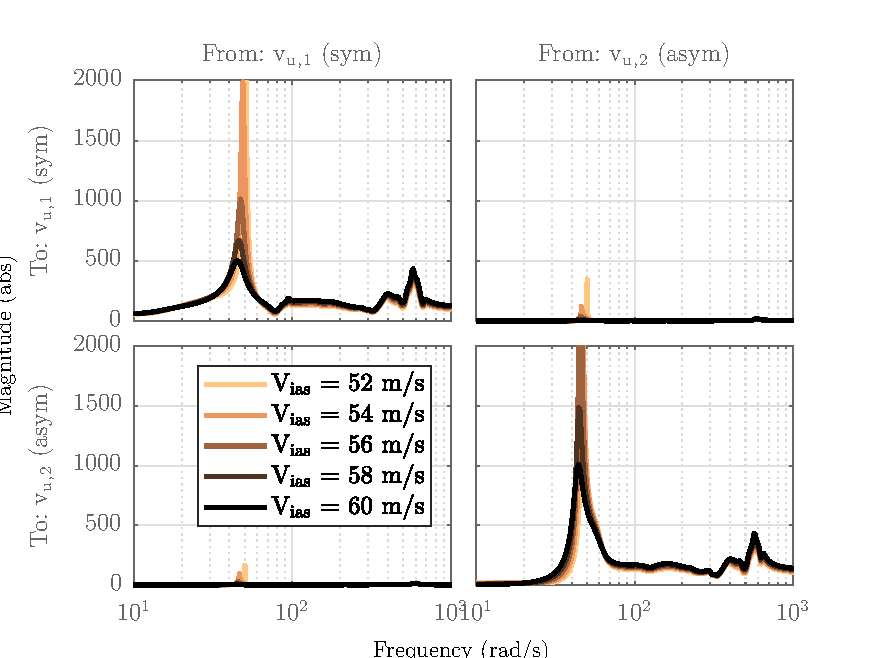
\includegraphics[width=0.75\linewidth]{figs/bode_v_1}
%	\caption{Bode-magnitude plots from virtual inputs to virtual outputs showing the decoupling of the two unstable flutter modes at different indicated airspeeds $V_{\text{ias}}$.}
%	\label{fig:bode}
%\end{figure}




\subsubsection{Single-Input Single-Output Controllers}
With the derived blending vectors it is possible to design dedicated SISO controllers for the symmetric ($j=1$) and asymmetric ($j=2$) flutter mode. 
The structure of the \ac{SISO} controllers is predefined as
%
\begin{align}
  c_j (V_{\text{ias}}(t))=W_{\text{BP},j} ~ W_{j}(V_{\text{ias}}(t)),
\end{align}
%
where $W_{\text{BP},j}$ denotes a bandpass filter to ensure that no interference with the baseline controller occurs and higher frequent modes are not excited. For both flutter modes, a second order Butterworth filter is chosen with a fixed passband from \SI{40}{\radian\per\second} to \SI{400}{\radian\per\second}. The corresponding corner frequencies are selected such that both flutter modes are well inside the passband and controller performance is affected as little as possible. 
Since a large velocity range needs to be considered, the core of the flutter suppression controller $W_{j}(V_{\text{ias}}(t))$ is gain-scheduled. For better tuning capabilities, it is desired to keep the order of $W_{j}(V_{\text{ias}}(t))$ as small as possible while a larger order may allow for a better controller performance. Hence, a careful balancing between controller order and performance is required. For the first (symmetric) and second (asymmetric) flutter mode, an order of two respectively one is chosen. 
The state space matrices $Z_j=\{A_j,B_j,C_j,D_j\}$ of $W_{j}(V_{\text{ias}}(t))$ depend linearly on the indicated airspeed, i.e. 
$Z_j=Z_j(V_{\text{ias}}(t)) = Z_{j,0}+Z_{j,1} V_{\text{ias}}(t)$, where the matrices $Z_{j,0}$ and $Z_{j,1}$ are subject to be optimized.
The two optimization problems to design the two SISO controllers have the form (\ref{eq:problem2}). As explicit optimization criteria a gain margin of \SI{6}{\decibel} and a phase margin of \SI{45}{\degree} are demanded in the optimization. The two problems are again solved using non-smooth optimization techniques \cite{Apkarian15}. The resulting \ac{SISO} controllers without the band-pass filter are depicted in Figure \ref{fig:sisoC}. Note that with increasing airspeed, the controller gain increases in the symmetric case and decreases in the asymmetric case in the frequency range of the corresponding flutter mode. 

Closing the two SISO loops stabilizes the two flutter modes as it is illustrated in the pole migration plot in Figure  \ref{fig:poles}. The plot compares the closed loop poles of the aircraft with the baseline controller depicted in gray to the closed-loop poles of the aircraft with baseline and flutter controller depicted in color in dependence of the airspeed. Clearly visible is the unstable behavior, i.e., the crossing to the right half plain of the first (symmetric) and second (asymmetric) flutter mode in the open-loop. With the flutter suppression controller the symmetric flutter mode is stabilized up to airspeeds of 65.5\,m/s. The asymmetric mode is stabilized even beyond  70\,m/s. Demanding additional single-loop robustness margins of 6\,dB in gain and \SI{45}{\degree} in phase to the critical point, leads to a maximum operational speed of about 60\,m/s. This still results in an increase in allowable speed of more than 15\,\% compared to the case without active flutter suppression. Also noticeable is that the other poles of the system(s) are not largely affected by the flutter suppression controller. This is acceptable since damping is increased rather than decreased.

%\begin{figure}[!htbp]
%  \centering
%  \begin{subfigure}[b]{0.49\textwidth}
%    \centering
%    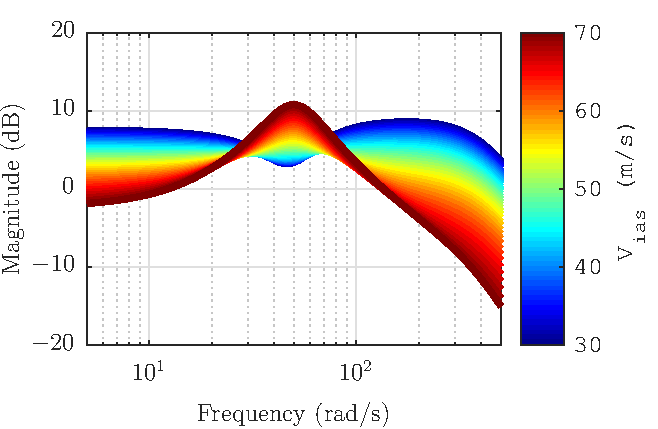
\includegraphics[width=\textwidth,trim={0cm 0cm 0cm 0cm},clip]{figs/sisoCFsym}
%    \caption{symmetric}
%  \end{subfigure}
%  \begin{subfigure}[b]{0.49\textwidth}
%    \centering
%    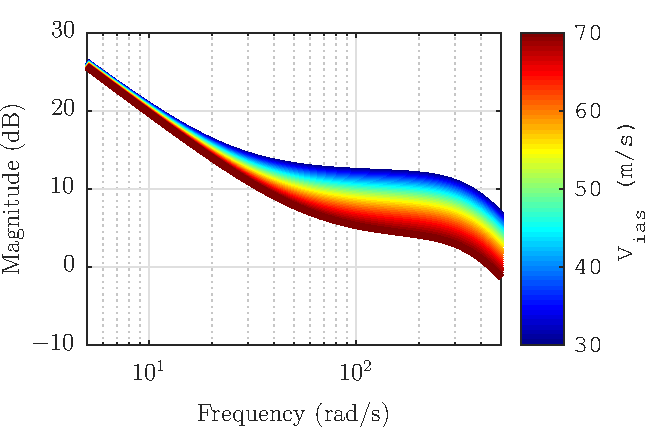
\includegraphics[width=\textwidth,trim={0cm 0cm 0cm 0cm},clip]{figs/sisoCFasym}
%    \caption{asymmetric}
%  \end{subfigure}
%  \caption{Gain-scheduled \ac{SISO} controllers $W_{j}(V_{\text{ias}}(t))$.}
%  \label{fig:sisoC}
%\end{figure}
%


\begin{figure}[h]
	\centering
	% This file was created by matlab2tikz.
%
%The latest updates can be retrieved from
%  http://www.mathworks.com/matlabcentral/fileexchange/22022-matlab2tikz-matlab2tikz
%where you can also make suggestions and rate matlab2tikz.
%
\definecolor{mycolor1}{rgb}{0.00000,0.00000,0.56250}%
\definecolor{mycolor2}{rgb}{0.00000,0.00000,0.66094}%
\definecolor{mycolor3}{rgb}{0.00000,0.00000,0.85781}%
\definecolor{mycolor4}{rgb}{0.00000,0.05469,1.00000}%
\definecolor{mycolor5}{rgb}{0.00000,0.15313,1.00000}%
\definecolor{mycolor6}{rgb}{0.00000,0.25156,1.00000}%
\definecolor{mycolor7}{rgb}{0.00000,0.35000,1.00000}%
\definecolor{mycolor8}{rgb}{0.00000,0.44844,1.00000}%
\definecolor{mycolor9}{rgb}{0.00000,0.54688,1.00000}%
\definecolor{mycolor10}{rgb}{0.00000,0.64531,1.00000}%
\definecolor{mycolor11}{rgb}{0.00000,0.74375,1.00000}%
\definecolor{mycolor12}{rgb}{0.00000,0.84219,1.00000}%
\definecolor{mycolor13}{rgb}{0.00000,0.94063,1.00000}%
\definecolor{mycolor14}{rgb}{0.03906,1.00000,0.96094}%
\definecolor{mycolor15}{rgb}{0.13750,1.00000,0.86250}%
\definecolor{mycolor16}{rgb}{0.23594,1.00000,0.76406}%
\definecolor{mycolor17}{rgb}{0.33437,1.00000,0.66563}%
\definecolor{mycolor18}{rgb}{0.43281,1.00000,0.56719}%
\definecolor{mycolor19}{rgb}{0.53125,1.00000,0.46875}%
\definecolor{mycolor20}{rgb}{0.62969,1.00000,0.37031}%
\definecolor{mycolor21}{rgb}{0.72813,1.00000,0.27187}%
\definecolor{mycolor22}{rgb}{0.82656,1.00000,0.17344}%
\definecolor{mycolor23}{rgb}{0.92500,1.00000,0.07500}%
\definecolor{mycolor24}{rgb}{1.00000,0.97656,0.00000}%
\definecolor{mycolor25}{rgb}{1.00000,0.87813,0.00000}%
\definecolor{mycolor26}{rgb}{1.00000,0.77969,0.00000}%
\definecolor{mycolor27}{rgb}{1.00000,0.68125,0.00000}%
\definecolor{mycolor28}{rgb}{1.00000,0.58281,0.00000}%
\definecolor{mycolor29}{rgb}{1.00000,0.48438,0.00000}%
\definecolor{mycolor30}{rgb}{1.00000,0.38594,0.00000}%
\definecolor{mycolor31}{rgb}{1.00000,0.28750,0.00000}%
\definecolor{mycolor32}{rgb}{1.00000,0.18906,0.00000}%
\definecolor{mycolor33}{rgb}{1.00000,0.09062,0.00000}%
\definecolor{mycolor34}{rgb}{0.99219,0.00000,0.00000}%
\definecolor{mycolor35}{rgb}{0.89375,0.00000,0.00000}%
\definecolor{mycolor36}{rgb}{0.79531,0.00000,0.00000}%
\definecolor{mycolor37}{rgb}{0.69688,0.00000,0.00000}%
\definecolor{mycolor38}{rgb}{0.59844,0.00000,0.00000}%
%
\begin{tikzpicture}

\begin{axis}[%
width=2in,
height=0.90in,
at={(0in,0in)},
scale only axis,
xmode=log,
xmin=5,
xmax=500,
xminorticks=true,
xlabel={Frequency (rad/s)},
xmajorgrids,
xminorgrids,
ymin=-20,
ymax=20,
ylabel={Magnitude (dB)},
ymajorgrids,
title={(a)},
title style = {yshift=-3mm, xshift=-23mm},
axis background/.style={fill=white}
]
\addplot [color=mycolor1,solid,line width=2.0pt,forget plot]
  table[row sep=crcr]{%
5	7.51539044714914\\
5.62667791300383	7.50264529016988\\
6.33190086733702	7.48642377824023\\
7.12551335151499	7.46575072407502\\
8.01859371875665	7.43936145151207\\
9.02360883413585	7.40560675198502\\
10.1545881045237	7.36232180450178\\
11.427319320675	7.3066432562896\\
12.8595690452967	7.23475126170031\\
14.4713306235838	7.14150306100352\\
16.2851032782989	7.01991246624248\\
18.3262061853981	6.8604214440438\\
20.5693940476824	6.65524849487193\\
22.9204258040832	6.40404942448797\\
25.2907209471365	6.11116577813245\\
27.6581847685353	5.77820143937397\\
30.0027872984	5.41065665454127\\
31.114665366668	5.22484662397677\\
32.3068523754468	5.01904312753329\\
34.5552042937082	4.61950054243777\\
36.7351954400362	4.23330167986537\\
38.8366396395257	3.88467270903657\\
40.8516750976247	3.59685471891658\\
42.7745786062422	3.38731778237372\\
44.7879938966807	3.25597045656323\\
47.1118148203396	3.2311010681324\\
49.8068556060415	3.3683788941607\\
52.9490307564103	3.70696408100212\\
56.6339473025277	4.24264190939709\\
60.9831532232063	4.91965617451846\\
63.7163938251719	5.32187384001553\\
66.152735266382	5.65234821685621\\
72.3452913329762	6.35891285790025\\
79.82681432627	6.98357148939966\\
88.9508252260718	7.50059987988053\\
95.724098808498	7.76818612538341\\
107.721734501594	8.09083059477069\\
121.223100854116	8.31326895008243\\
136.416668824338	8.46162747372885\\
153.514531487892	8.55108419849005\\
172.755364729611	8.58768958724238\\
194.407759015404	8.56917335417544\\
218.773968753709	8.48471230945895\\
246.194131585337	8.31409636166308\\
277.051016500475	8.02726602417223\\
311.775367063696	7.58591556482383\\
350.851914335191	6.94915561279929\\
394.826143424986	6.0837241510816\\
444.31190813717	4.97533871352363\\
500	3.63457386669532\\
};
\addplot [color=mycolor2,solid,line width=2.0pt,forget plot]
  table[row sep=crcr]{%
5	7.36184756718134\\
5.62667791300383	7.34959122169383\\
6.33190086733702	7.33399178521977\\
7.12551335151499	7.31411142013807\\
8.01859371875665	7.28873387287447\\
9.02360883413585	7.25627306376993\\
10.1545881045237	7.21464702471933\\
11.427319320675	7.16110200220306\\
12.8595690452967	7.09196445537555\\
14.4713306235838	7.00228892887381\\
16.2851032782989	6.88535823010914\\
18.3262061853981	6.7319849939988\\
20.4601138762059	6.54504078926235\\
22.8062701511087	6.30577401485438\\
25.173422059673	6.02653556649739\\
27.5395364623346	5.70873735870528\\
29.8845853756405	5.35749397251306\\
31.1714574269369	5.15136394238008\\
32.190842833525	4.98270016702778\\
34.4430406254683	4.59963850620188\\
36.6284054653079	4.22853334573813\\
38.7366016364378	3.89250733594591\\
40.7596025221746	3.61386819992076\\
42.6915123830433	3.4095740194361\\
44.7149902543824	3.27957218952892\\
47.05020968688	3.25096610534236\\
49.7582465411374	3.3779320929485\\
52.915340703221	3.69958200744732\\
56.6175057601609	4.21350068236707\\
60.9867999385779	4.86658786330827\\
63.6416766549178	5.24312585480226\\
66.1799530302274	5.57532603186874\\
72.4003762869898	6.25915515627795\\
79.9150942909853	6.86303195535859\\
89.0789386891483	7.36175376373078\\
95.724098808498	7.61412300613098\\
107.721734501594	7.92475577442163\\
121.223100854116	8.1383676153356\\
136.416668824338	8.28019510694753\\
153.514531487892	8.36477935592303\\
172.755364729611	8.39771891341534\\
194.407759015404	8.37642274907978\\
218.773968753709	8.28983860785676\\
246.194131585337	8.1175912527383\\
277.051016500475	7.82950083297142\\
311.775367063696	7.38717291296149\\
350.851914335191	6.7496520576685\\
394.826143424986	5.8836265719334\\
444.31190813717	4.77477631521161\\
500	3.4336470734659\\
};
\addplot [color=blue!45!mycolor1,solid,line width=2.0pt,forget plot]
  table[row sep=crcr]{%
5	7.20587592236311\\
5.62667791300383	7.19412994564348\\
6.33190086733702	7.17918012832747\\
7.12551335151499	7.16012772700397\\
8.01859371875665	7.13580721302986\\
9.02360883413585	7.10469870315775\\
10.1545881045237	7.06480721540285\\
11.427319320675	7.01349423820061\\
12.8595690452967	6.94724035466563\\
14.4713306235838	6.86130842827319\\
16.2851032782989	6.74926604639258\\
18.3262061853981	6.60231950724791\\
20.3374838922678	6.43426735263215\\
22.677806648509	6.20754888808299\\
25.0410106587485	5.94270541072736\\
27.4051396791526	5.64096031712712\\
29.7501768974844	5.30703130426745\\
31.2330560433556	5.08042548330663\\
32.0583499763417	4.95016461529334\\
34.3142964994078	4.58473086677323\\
36.5051114290679	4.22983060971686\\
38.6202998753146	3.90739689598564\\
40.6516580441696	3.63872296590219\\
42.5931033760684	3.44019589888979\\
44.6272684187514	3.31179110541407\\
46.9745823067531	3.27932393822641\\
49.6963954959985	3.39530960489377\\
52.8692889051583	3.69873473800496\\
56.5897014831789	4.18910178508734\\
60.9802241329817	4.81625884156971\\
63.5546004043005	5.16664829345829\\
66.198256109766	5.49913664591371\\
72.4480525138325	6.15861207838495\\
79.9977036281737	6.74044243794622\\
89.2033874403799	7.21993013485041\\
95.724098808498	7.45715931497882\\
107.721734501594	7.75516830922955\\
121.223100854116	7.95955754850823\\
136.416668824338	8.09459169249518\\
153.514531487892	8.17412535403827\\
172.755364729611	8.20327520990781\\
194.407759015404	8.17911107972655\\
218.773968753709	8.09034008263166\\
246.194131585337	7.91641439387124\\
277.051016500475	7.62702888692797\\
311.775367063696	7.18369710258854\\
350.851914335191	6.54539524640029\\
394.826143424986	5.67876032573811\\
444.31190813717	4.56943336217209\\
500	3.22793051161453\\
};
\addplot [color=mycolor3,solid,line width=2.0pt,forget plot]
  table[row sep=crcr]{%
5	7.04739686392819\\
5.62667791300383	7.03618455378693\\
6.33190086733702	7.02191411185255\\
7.12551335151499	7.00372776409582\\
8.01859371875665	6.98051317737031\\
9.02360883413585	6.9508199496837\\
10.1545881045237	6.91274450012931\\
11.427319320675	6.86376956803257\\
12.8595690452967	6.80053815638246\\
14.4713306235838	6.71853308123088\\
16.2851032782989	6.61162329064519\\
18.3262061853981	6.47143273592668\\
20.2005081023499	6.32279170300652\\
22.5339026746507	6.10922935905073\\
24.8922186289646	5.85952408660428\\
27.2535946078102	5.57471594935148\\
29.5980365787843	5.25911676908507\\
31.3014952794176	5.01208611375505\\
31.9077313697957	4.92129527160694\\
34.1672223882764	4.5746579252023\\
36.3634681004725	4.23710831237938\\
38.485805746901	3.92930483637724\\
40.5258425565082	3.67144386814374\\
42.4772950680481	3.47927793749757\\
44.5227164316726	3.35279915191965\\
46.8827548567906	3.31643090587153\\
49.6190459972815	3.42084142609286\\
52.8085243744347	3.70478545376924\\
56.5480690365225	4.16977763621778\\
60.960820542784	4.768913131126\\
63.4503681019594	5.09251099987691\\
66.2048666336642	5.42391049275737\\
72.4853265670147	6.05730764679597\\
80.0713761104407	6.61574387725043\\
89.3205550650545	7.07501185209956\\
95.724098808498	7.29728662627293\\
107.721734501594	7.58199963846033\\
121.223100854116	7.77672738676002\\
136.416668824338	7.90467505986979\\
153.514531487892	7.97895752808523\\
172.755364729611	8.00417715969309\\
194.407759015404	7.97704455157507\\
218.773968753709	7.88601349423958\\
246.194131585337	7.71035533582866\\
277.051016500475	7.41963419575151\\
311.775367063696	6.97526786128946\\
350.851914335191	6.33616158269838\\
394.826143424986	5.46889922699357\\
444.31190813717	4.35908164629377\\
500	3.01719438948071\\
};
\addplot [color=blue!90!mycolor1,solid,line width=2.0pt,forget plot]
  table[row sep=crcr]{%
5	6.88632799371932\\
5.62667791300383	6.87567457932934\\
6.33190086733702	6.86211572305534\\
7.12551335151499	6.84483663942114\\
8.01859371875665	6.82278084635807\\
9.02360883413585	6.79457094628187\\
10.1545881045237	6.75839948198446\\
11.427319320675	6.71187685039718\\
12.8595690452967	6.65181728425258\\
14.4713306235838	6.57393584641285\\
16.2851032782989	6.47242026207637\\
18.3262061853981	6.33933714272045\\
20.0480636751771	6.21045483283055\\
22.3732765935178	6.01064228023133\\
24.7256054388156	5.77680480877751\\
27.0833047640669	5.50980629417125\\
29.4264177369027	5.21354648025265\\
31.3794854648863	4.94639745672816\\
31.7370983775384	4.89589110023733\\
33.9997980479041	4.56923418926053\\
36.2013356478353	4.25021280076338\\
38.3308730892255	3.95812777654067\\
40.3798176352478	3.71199540961434\\
42.3416712554586	3.52686517065382\\
44.3988415425721	3.40273416147498\\
46.7721442329805	3.36253016031778\\
49.5235076999854	3.45486945826244\\
52.7302286378093	3.71813354237655\\
56.4896356742612	4.15591298386781\\
60.9254290051425	4.72485063986034\\
63.3227090075273	5.02079222841706\\
66.1963944327787	5.34982709726472\\
72.5085227596031	5.95530344650513\\
80.132077088108	6.48890291021516\\
89.4259492464174	6.92689724226469\\
95.724098808498	7.13451152291266\\
107.721734501594	7.40518857266539\\
121.223100854116	7.58976720182911\\
136.416668824338	7.71029996670447\\
153.514531487892	7.77910473955081\\
172.755364729611	7.80023439888455\\
194.407759015404	7.77001836762499\\
218.773968753709	7.67664310606885\\
246.194131585337	7.49918998382259\\
277.051016500475	7.20708623677639\\
311.775367063696	6.76164969663246\\
350.851914335191	6.12171171517855\\
394.826143424986	5.2538009175488\\
444.31190813717	4.14347646018827\\
500	2.80119216013985\\
};
\addplot [color=mycolor4,solid,line width=2.0pt,forget plot]
  table[row sep=crcr]{%
5	6.72258293582606\\
5.62667791300383	6.71251579235217\\
6.33190086733702	6.6997034575358\\
7.12551335151499	6.68337631249004\\
8.01859371875665	6.66253658540698\\
9.02360883413585	6.63588366764664\\
10.1545881045237	6.60171128428864\\
11.427319320675	6.55776432838315\\
12.8595690452967	6.50103762559263\\
14.4713306235838	6.42749148251223\\
16.2851032782989	6.33165069105964\\
18.3262061853981	6.20605056109138\\
20.6231319145068	6.04051680359308\\
22.1944680077951	5.91158166881012\\
24.5395241657754	5.69431947241986\\
26.8924385197931	5.44598237537163\\
29.2333091030665	5.17005525487971\\
31.4706918370386	4.8834102339133\\
31.5442680852045	4.87368001008518\\
33.809679441676	4.56819540605756\\
36.0162215089558	4.26890769742762\\
38.1528750068979	3.99368078736397\\
40.2108373657579	3.76026751247659\\
42.1833829898527	3.58294045220787\\
44.2526919865612	3.4616898427001\\
46.639677878715	3.4178458908036\\
49.4065653174118	3.49774765411916\\
52.6310166157666	3.7392217711422\\
56.410812755653	4.1479584648839\\
60.870214664885	4.68444438728225\\
63.1633218477241	4.95158561764047\\
66.1687038592245	5.27713256839371\\
72.5131338508317	5.85271395930979\\
80.1748345508269	6.35992403473335\\
85.0627139926295	6.59974509060644\\
95.724098808498	6.96885862565667\\
107.721734501594	7.2246834217261\\
121.223100854116	7.39856981101018\\
136.416668824338	7.51131873480269\\
153.514531487892	7.57438947531694\\
172.755364729611	7.59124719544202\\
194.407759015404	7.55781607972778\\
218.773968753709	7.46199978112139\\
246.194131585337	7.28267949598929\\
277.051016500475	6.9891386989086\\
311.775367063696	6.54259051940834\\
350.851914335191	5.901789066151\\
394.826143424986	5.033205321353\\
444.31190813717	3.92235499383267\\
500	2.5796588723864\\
};
\addplot [color=mycolor5,solid,line width=2.0pt,forget plot]
  table[row sep=crcr]{%
5	6.5560710920726\\
5.62667791300383	6.54661998241349\\
6.33190086733702	6.53459213588486\\
7.12551335151499	6.51926545361916\\
8.01859371875665	6.49970395742135\\
9.02360883413585	6.47468789887995\\
10.1545881045237	6.44261761074854\\
11.427319320675	6.40137978904819\\
12.8595690452967	6.34815981023543\\
14.4713306235838	6.27917696679718\\
16.2851032782989	6.18931231404313\\
18.3262061853981	6.07159693155871\\
20.6231319145068	5.91655235491747\\
21.9958005793033	5.81180345994292\\
24.3320791285524	5.61179176502064\\
26.6788812092809	5.38293533508799\\
29.0163811160007	5.12830548750728\\
31.3267035542337	4.85430533773499\\
31.5801650675352	4.82317828011805\\
33.5941327927652	4.57118278473819\\
35.8052081482432	4.29285634239844\\
37.9487253080207	4.03567890396004\\
40.0156635004732	3.81605725794409\\
41.9990575593809	3.64740773458309\\
44.0807594220031	3.52970209978294\\
46.4816886880618	3.48257471052799\\
49.2643647977992	3.5498408054047\\
52.5068126258067	3.76854422068579\\
56.3072598054385	4.14644726342748\\
60.7905179086408	4.64816260075524\\
62.9610415365933	4.88501059540127\\
66.1167468770229	5.20616260931986\\
72.4936338796596	5.74972703963694\\
80.1935273743086	6.22886599905985\\
85.0627139926295	6.45341604604099\\
95.724098808498	6.80037411889525\\
107.721734501594	7.04044454632976\\
121.223100854116	7.20303240742802\\
136.416668824338	7.30758210264422\\
153.514531487892	7.36462807325603\\
172.755364729611	7.37700617951958\\
194.407759015404	7.34020893097436\\
218.773968753709	7.24184002136931\\
246.194131585337	7.06056908612804\\
277.051016500475	6.76552810044996\\
311.775367063696	6.31782011676032\\
350.851914335191	5.67611819137191\\
394.826143424986	4.80683291525196\\
444.31190813717	3.69543453549197\\
500	2.35230931671649\\
};
\addplot [color=mycolor6,solid,line width=2.0pt,forget plot]
  table[row sep=crcr]{%
5	6.3866973801778\\
5.62667791300383	6.37789472764367\\
6.33190086733702	6.36669271158091\\
7.12551335151499	6.35241930034705\\
8.01859371875665	6.3342036396311\\
9.02360883413585	6.31091122713343\\
10.1545881045237	6.28105482896133\\
11.427319320675	6.24267075837663\\
12.8595690452967	6.19314553825516\\
14.4713306235838	6.12897197643859\\
16.2851032782989	6.04540752393371\\
18.3262061853981	5.93600712128406\\
20.6231319145068	5.79202725655011\\
21.7753352001238	5.71101915292323\\
24.1010726273518	5.5288888593056\\
26.4401750106467	5.32028576080298\\
28.7729185732333	5.08787373650332\\
31.0814389395835	4.83730945713061\\
31.7150316415169	4.7657653230696\\
33.3499519404063	4.57772366350285\\
35.5648625039661	4.32159995022446\\
37.714779976504	4.08371367715112\\
39.7904589705104	3.87904517955758\\
41.7846841300525	3.7200697475702\\
43.8788562138031	3.6067300328753\\
46.293782674484	3.55687265616822\\
49.092269867585	3.61152078421959\\
52.3526939699388	3.80665447906256\\
56.1737129108494	4.15201530610045\\
60.6806648204426	4.61659700576618\\
62.70054903164	4.82122797449965\\
66.0343521608768	5.1373728740566\\
72.4432416284578	5.64663140998552\\
80.1806177403108	6.09586404501736\\
85.0627139926295	6.30580862237874\\
95.724098808498	6.6291298411751\\
107.721734501594	6.85244740966774\\
121.223100854116	7.00305857821498\\
136.416668824338	7.09894034857886\\
153.514531487892	7.14963111308155\\
172.755364729611	7.15729215007802\\
194.407759015404	7.11695520154368\\
218.773968753709	7.01590495197775\\
246.194131585337	6.83258672456512\\
277.051016500475	6.53597226794401\\
311.775367063696	6.08704845696201\\
350.851914335191	5.44440294822399\\
394.826143424986	4.57438278987323\\
444.31190813717	3.46241044825008\\
500	2.11883593548835\\
};
\addplot [color=mycolor7,solid,line width=2.0pt,forget plot]
  table[row sep=crcr]{%
5	6.21436195334655\\
5.62667791300383	6.20624314969529\\
6.33190086733702	6.19591207022412\\
7.12551335151499	6.18274951194013\\
8.01859371875665	6.1659533467581\\
9.02360883413585	6.14447904950927\\
10.1545881045237	6.11695808191591\\
11.427319320675	6.08158473772845\\
12.8595690452967	6.03595796401363\\
14.4713306235838	5.97685944121347\\
16.2851032782989	5.8999441048106\\
18.3262061853981	5.79931983451678\\
20.6231319145068	5.66701791419552\\
21.5308104895952	5.6088880478566\\
23.8439373818873	5.4452113143334\\
26.173442779088	5.25757074507349\\
28.4997353771862	5.04823444552827\\
30.8049847435841	4.82211377598424\\
31.8856513172659	4.71125655115435\\
33.0733537843711	4.58720765674421\\
35.2911214009981	4.35453022507149\\
37.4467124286285	4.13722316196433\\
39.5306529590589	3.94876415787685\\
41.5354687028779	3.80059783558839\\
43.6419596244589	3.69262920477347\\
46.0706707873456	3.6408354189313\\
48.8846795420605	3.68315826142392\\
52.1626918036655	3.85417302895596\\
56.0037661024021	4.16542527023799\\
60.5337255779837	4.59049895393072\\
62.3602901925174	4.76046359193093\\
65.9139561779828	5.07137918053003\\
72.3536189823357	5.54385386791933\\
80.1268099592187	5.96116039481241\\
85.0627139926295	6.15716217675651\\
95.724098808498	6.45522801322634\\
107.721734501594	6.66068621821894\\
121.223100854116	6.7985607932261\\
136.416668824338	6.88524475185797\\
153.514531487892	6.92920402181466\\
172.755364729611	6.93187599019143\\
194.407759015404	6.88779957557063\\
218.773968753709	6.78391925542003\\
246.194131585337	6.59844173184958\\
277.051016500475	6.30016866237197\\
311.775367063696	5.84996380542927\\
350.851914335191	5.20632444651545\\
394.826143424986	4.33553047048798\\
444.31190813717	3.22295388861654\\
500	1.87890646101245\\
};
\addplot [color=mycolor8,solid,line width=2.0pt,forget plot]
  table[row sep=crcr]{%
5	6.03895989999573\\
5.62667791300383	6.03156365395412\\
6.33190086733702	6.02215282037275\\
7.12551335151499	6.01016402328666\\
8.01859371875665	5.99486776303341\\
9.02360883413585	5.97531460114922\\
10.1545881045237	5.9502614329854\\
11.427319320675	5.91806948890386\\
12.8595690452967	5.87656214515795\\
14.4713306235838	5.82282617725231\\
16.2851032782989	5.75293606062844\\
18.3262061853981	5.66158262164134\\
20.6231319145068	5.54161229252278\\
21.2595664230592	5.50500767896322\\
23.5576499391293	5.36028070095933\\
25.8752905323148	5.19422808265703\\
28.19306546809	5.00874005642796\\
30.4932066549198	4.80799416662464\\
32.1076665077373	4.65977894231269\\
32.7598445913713	4.59885703375635\\
34.9791449985359	4.39085478355136\\
37.1393538938993	4.19545319578477\\
39.2307681262745	4.02455822931082\\
41.2456482100863	3.88849077449755\\
43.3640119101015	3.78711362332753\\
45.8059529288054	3.73446813995952\\
48.6347935703233	3.76510663658141\\
51.929534999024	3.9117917367033\\
55.7895899739927	4.18759424576469\\
60.3412033429172	4.57082535840749\\
61.9089441356543	4.70304474485928\\
65.7462568061072	5.00901103848421\\
72.2144823726452	5.442010118277\\
80.0206110706466	5.82514655295811\\
85.0627139926295	6.00776402195693\\
95.724098808498	6.27880667864917\\
107.721734501594	6.46517825355033\\
121.223100854116	6.58946346351125\\
136.416668824338	6.66634947459614\\
153.514531487892	6.70314795659761\\
172.755364729611	6.70051873363122\\
194.407759015404	6.65247255353876\\
218.773968753709	6.54559006454793\\
246.194131585337	6.35782326151342\\
277.051016500475	6.05779253844676\\
311.775367063696	5.60623062923585\\
350.851914335191	4.96153875235938\\
394.826143424986	4.08992546286929\\
444.31190813717	2.97670922789293\\
500	1.63216123880902\\
};
\addplot [color=mycolor9,solid,line width=2.0pt,forget plot]
  table[row sep=crcr]{%
5	5.86038092227229\\
5.62667791300383	5.85374965449553\\
6.33190086733702	5.84531307647115\\
7.12551335151499	5.83456689987216\\
8.01859371875665	5.8208584861743\\
9.02360883413585	5.80333900823863\\
10.1545881045237	5.78089805090842\\
11.427319320675	5.75207337612206\\
12.8595690452967	5.71492556645887\\
14.4713306235838	5.66686361266982\\
16.2851032782989	5.60440454836836\\
18.3262061853981	5.52285299458847\\
20.6231319145068	5.41591112875388\\
20.9584451724697	5.39890192850638\\
23.238618378614	5.27352432006782\\
25.541681111074	5.12957683114576\\
27.8484216106721	4.96859655102153\\
30.1411687351082	4.79405060123273\\
32.4040469759097	4.61168971044402\\
32.4058896470739	4.61153875375222\\
34.6231270944018	4.42955322016744\\
36.7864867148255	4.25740709068938\\
38.8841967228928	4.10552761131026\\
40.9082494059251	3.98301805276291\\
43.0376608107251	3.88970120633339\\
45.4918373268555	3.83763910596644\\
48.3343074383352	3.85767279176429\\
51.6443168565178	3.98027151398893\\
55.5215653435532	4.21962389107463\\
60.0926290492547	4.55879662345912\\
61.2990318620366	4.64945751601314\\
65.5197620775167	4.95138325563432\\
72.0130965702092	5.34197500017605\\
79.8477585377184	5.68842286387344\\
85.0627139926295	5.85795566631735\\
95.724098808498	6.10004593143647\\
107.721734501594	6.26596901071867\\
121.223100854116	6.37570668819643\\
136.416668824338	6.44211396735493\\
153.514531487892	6.47126104453403\\
172.755364729611	6.46297183852545\\
194.407759015404	6.41068994402003\\
218.773968753709	6.3006058293749\\
246.194131585337	6.1103986706489\\
277.051016500475	5.8084949225843\\
311.775367063696	5.35548726500404\\
350.851914335191	4.70967431137212\\
394.826143424986	3.8371884834659\\
444.31190813717	2.72329113009225\\
500	1.37821018542603\\
};
\addplot [color=mycolor10,solid,line width=2.0pt,forget plot]
  table[row sep=crcr]{%
5	5.67850899198988\\
5.62667791300383	5.6726892833879\\
6.33190086733702	5.66528623464954\\
7.12551335151499	5.65585819602272\\
8.01859371875665	5.6438339871481\\
9.02360883413585	5.6284713716081\\
10.1545881045237	5.60880044244031\\
11.427319320675	5.58354577457467\\
12.8595690452967	5.55101874980072\\
14.4713306235838	5.50896861718357\\
16.2851032782989	5.45437892685636\\
18.3262061853981	5.38319965615714\\
20.6231319145068	5.29002923450476\\
20.6236606346148	5.29000614058289\\
22.8825347102555	5.18425618284647\\
25.1677682542664	5.06279322159079\\
27.4604100462533	4.92683316801862\\
29.7429276671691	4.77916939644854\\
31.999472908768	4.62447275428802\\
32.8223748752387	4.56689566770463\\
34.2160462186776	4.46932098027369\\
36.3805730256551	4.32177990082675\\
38.4829065351542	4.19045486768833\\
40.5147719407196	4.08314120839653\\
42.6539181469845	3.99963500557184\\
45.1187710608901	3.95000857211277\\
47.9730105260526	3.96106577161198\\
51.2960557221791	4.06042592285553\\
55.1878000638246	4.26282978423165\\
59.7750267619358	4.55596856799072\\
60.4543270026983	4.60043876814305\\
65.2201946881113	4.89999212555816\\
71.7336067089132	5.24498072570768\\
79.5904652665547	5.55188378216851\\
85.0627139926295	5.70813947820154\\
95.724098808498	5.91917499829632\\
107.721734501594	6.06313827234542\\
121.223100854116	6.157250830906\\
136.416668824338	6.21240602503752\\
153.514531487892	6.23334008070859\\
172.755364729611	6.21897774109346\\
194.407759015404	6.1621524810697\\
218.773968753709	6.04863518030636\\
246.194131585337	5.85581178101156\\
277.051016500475	5.55190039564242\\
311.775367063696	5.09734332267268\\
350.851914335191	4.45032905269139\\
394.826143424986	3.57690832654314\\
444.31190813717	2.46228123198001\\
500	1.11662932073559\\
};
\addplot [color=mycolor11,solid,line width=2.0pt,forget plot]
  table[row sep=crcr]{%
5	5.49322198260368\\
5.62667791300383	5.48826508411213\\
6.33190086733702	5.4819607425519\\
7.12551335151499	5.47393381921519\\
8.01859371875665	5.46369959042461\\
9.02360883413585	5.4506288877616\\
10.1545881045237	5.4339007417526\\
11.427319320675	5.41243755678981\\
12.8595690452967	5.38481596323358\\
14.4713306235838	5.34914444917313\\
16.2851032782989	5.30289793314585\\
18.3262061853981	5.24270385026713\\
20.2506240923935	5.17764832910102\\
22.4841778224501	5.09165315087246\\
24.7476752507675	4.99288058030279\\
27.0224833719327	4.88226464995542\\
29.2912585277516	4.76197599001388\\
31.5382212202913	4.63566367801218\\
33.4354212825446	4.52652490061808\\
33.7493339038129	4.50849734142869\\
35.9123930404208	4.38687216739379\\
38.0170486681795	4.27770528222559\\
40.0547653470079	4.18740415710109\\
42.2017037936651	4.11576880157336\\
44.6749462002731	4.07091910075313\\
47.5382486533342	4.07530866420829\\
50.8711070227264	4.1530775498809\\
54.7734821801462	4.31876223405944\\
59.2419627040502	4.55712419965884\\
59.3721977703307	4.56431903498065\\
64.8296945368275	4.8568448538689\\
71.3561438480489	5.15275614183605\\
79.2264090076362	5.41684228510522\\
85.0627139926295	5.55878567175593\\
95.724098808498	5.73648022982094\\
107.721734501594	5.85680725952613\\
121.223100854116	5.93408209241754\\
136.416668824338	5.97710564900847\\
153.514531487892	5.98918281270685\\
172.755364729611	5.96827078485842\\
194.407759015404	5.90654563031976\\
218.773968753709	5.78932582167509\\
246.194131585337	5.59368103937805\\
277.051016500475	5.28760466810762\\
311.775367063696	4.83137679549737\\
350.851914335191	4.18306713007225\\
394.826143424986	3.30863831317089\\
444.31190813717	2.19322436098296\\
500	0.846956803152611\\
};
\addplot [color=mycolor12,solid,line width=2.0pt,forget plot]
  table[row sep=crcr]{%
5	5.30439127586793\\
5.62667791300383	5.30035368910364\\
6.33190086733702	5.29521986482998\\
7.12551335151499	5.28868540401576\\
8.01859371875665	5.2803574804853\\
9.02360883413585	5.26972701553433\\
10.1545881045237	5.25613106730705\\
11.427319320675	5.23870166986306\\
12.8595690452967	5.21629604378603\\
14.4713306235838	5.18740183504501\\
16.2851032782989	5.15001099889535\\
18.3262061853981	5.10146083921984\\
19.8337070363818	5.06102526324706\\
22.0371456152381	4.99472475867293\\
24.274194250154	4.91863147561534\\
26.5266050215328	4.8334438429936\\
28.7772826020095	4.74077553003096\\
31.010567123681	4.64333598749748\\
33.2124245347564	4.54497270457813\\
34.4137202686642	4.49182967938112\\
35.3705541175781	4.45047643543003\\
37.4744249988066	4.36509206640587\\
39.5152543484361	4.2937797898827\\
41.6672257485291	4.23640035260264\\
44.1456280563499	4.19922631434046\\
47.0141926732136	4.20008926784164\\
50.3523627927851	4.25896321990409\\
54.2599990352308	4.38920172746555\\
57.3985709115312	4.52126516480879\\
58.8637454719177	4.5863457442786\\
64.3257325096052	4.82463304453616\\
70.8556068686995	5.06772679495786\\
78.727356583283	5.28521523402575\\
85.0627139926295	5.41043945157245\\
95.724098808498	5.55231402969087\\
107.721734501594	5.64714700948854\\
121.223100854116	5.70621927459586\\
136.416668824338	5.73610990667793\\
153.514531487892	5.73859097426003\\
172.755364729611	5.71057864991704\\
194.407759015404	5.64353966924467\\
218.773968753709	5.52230350490494\\
246.194131585337	5.32359759486432\\
277.051016500475	5.0151719386694\\
311.775367063696	4.55713084502413\\
350.851914335191	3.90741525064073\\
394.826143424986	3.03189225791765\\
444.31190813717	1.91562421497217\\
500	0.568688382283652\\
};
\addplot [color=mycolor13,solid,line width=2.0pt,forget plot]
  table[row sep=crcr]{%
5	5.111881341891\\
5.62667791300383	5.10882548174437\\
6.33190086733702	5.10494144655743\\
7.12551335151499	5.10000020015351\\
8.01859371875665	5.09370674165569\\
9.02360883413585	5.08567969823054\\
10.1545881045237	5.07542395886977\\
11.427319320675	5.06229381870358\\
12.8595690452967	5.04544335071863\\
14.4713306235838	5.02376019721026\\
16.2851032782989	4.99577971947978\\
18.3262061853981	4.95958151256626\\
19.3659116108459	4.93917177745264\\
21.5334830691246	4.89227471549306\\
23.7383690255726	4.83857967887383\\
25.9627839487819	4.77860173895745\\
28.1899514247289	4.71347769430058\\
30.4043933145561	4.64508440110558\\
32.5921315144991	4.5760690237494\\
34.7408103412603	4.50972784935914\\
36.2341875274507	4.4663126859135\\
36.8397498894211	4.44969393244732\\
38.8799418045552	4.39945524672456\\
41.0331199115899	4.35902802129911\\
43.5122226533176	4.33303752504038\\
46.3808227471442	4.33450908011953\\
49.7181397137728	4.37854459608551\\
53.6237133562261	4.47609362077462\\
54.2604483760151	4.49527861994317\\
58.2237204495367	4.62516094129811\\
63.6796012858822	4.80696164893527\\
70.1999704308428	4.99330579202539\\
78.0572536476412	5.15980590619398\\
85.0627139926295	5.26372807917875\\
95.724098808498	5.36710471121869\\
107.721734501594	5.43438813242105\\
121.223100854116	5.47372196099287\\
136.416668824338	5.48933902205029\\
153.514531487892	5.48137427382067\\
172.755364729611	5.44562444483565\\
194.407759015404	5.37279015715472\\
218.773968753709	5.24717115209163\\
246.194131585337	5.04512332412002\\
277.051016500475	4.73413203292775\\
311.775367063696	4.27411022919894\\
350.851914335191	3.62285853593671\\
394.826143424986	2.74613987872169\\
444.31190813717	1.62893841390846\\
500	0.281272166554157\\
};
\addplot [color=mycolor14,solid,line width=2.0pt,forget plot]
  table[row sep=crcr]{%
5	4.91554929143672\\
5.62667791300383	4.91354424357114\\
6.33190086733702	4.91099767760526\\
7.12551335151499	4.90776098041145\\
8.01859371875665	4.90364343991247\\
9.02360883413585	4.89839965306754\\
10.1545881045237	4.89171290961455\\
11.427319320675	4.88317327284534\\
12.8595690452967	4.87224886807538\\
14.4713306235838	4.85824904840657\\
16.2851032782989	4.84027948855069\\
17.9338054289738	4.82186962370005\\
18.8384010857593	4.81092103118531\\
19.9863084536925	4.79616369161285\\
20.9631526840202	4.78285133344284\\
22.0869699443749	4.76669525698312\\
23.1289012726051	4.7509386422534\\
24.2196149084833	4.7336833035302\\
25.3184128770731	4.71557102070152\\
26.3686506537486	4.69764744749273\\
27.5153133421651	4.67750098121909\\
28.5193641756023	4.65947471918932\\
29.7043815434211	4.6379037994427\\
30.6581491245198	4.62045738393778\\
31.87176094207	4.59838553291069\\
32.7726657601308	4.58227270259518\\
34.0050958444256	4.56090781008997\\
34.8519398949874	4.54687767781131\\
36.0936011768015	4.52760889415081\\
38.1280758900364	4.50053216168402\\
40.2772270895136	4.47999625573058\\
42.750950555391	4.46930875040095\\
43.4799550237468	4.46911996806268\\
44.7852957699152	4.47230261793996\\
45.6124835310702	4.47666392485556\\
48.9405971624529	4.51164530799675\\
52.834221911208	4.58134867109269\\
57.4186927962142	4.68454086525851\\
62.8542685163457	4.80863860279224\\
69.347878775149	4.93431989497345\\
77.1695094747358	5.04474516433554\\
85.0627139926295	5.11936753312326\\
95.724098808498	5.18136721066445\\
107.721734501594	5.21883209192023\\
121.223100854116	5.23670037016035\\
136.416668824338	5.23674398057828\\
153.514531487892	5.2173555979815\\
172.755364729611	5.17312967317087\\
194.407759015404	5.09393895083031\\
218.773968753709	4.96350823055523\\
246.194131585337	4.75778885457838\\
277.051016500475	4.44397732863004\\
311.775367063696	3.98177734302288\\
350.851914335191	3.32883585398891\\
394.826143424986	2.45080156357893\\
444.31190813717	1.33257281662684\\
500	-0.0158974173210274\\
};
\addplot [color=mycolor15,solid,line width=2.0pt,forget plot]
  table[row sep=crcr]{%
5	4.71524439953846\\
5.62667791300383	4.71436678804868\\
6.33190086733702	4.71325486201975\\
7.12551335151499	4.71184597547548\\
8.01859371875665	4.71006075724629\\
9.02360883413585	4.70779874211746\\
10.1545881045237	4.70493301094273\\
11.427319320675	4.7013038171093\\
12.8595690452967	4.69671147774794\\
14.4713306235838	4.69090957142887\\
16.2851032782989	4.68360131026664\\
18.1493388148445	4.67527633978402\\
18.2398104496245	4.67485254248364\\
20.2217557490118	4.66514913609075\\
20.3132573942855	4.6646830411062\\
22.3414047927057	4.65400824765268\\
22.4312799342931	4.65352191244066\\
24.4918691535564	4.64216444762012\\
24.577298389841	4.64168770046277\\
26.657360154788	4.63008222902261\\
26.7354390848154	4.6296500805498\\
28.8230156419332	4.61838686157691\\
28.8908288380362	4.61803419381626\\
30.9751258522178	4.60784659646711\\
31.0298141809348	4.60759996425865\\
33.1012906148537	4.59931976743984\\
33.1401100154491	4.59918720605296\\
35.1905143436852	4.59366318394397\\
35.2108849564634	4.59362433835614\\
37.2327920792461	4.59161136983666\\
39.370802742687	4.59398271520713\\
39.3945555466832	4.59403766854149\\
41.8309053702634	4.6032269504199\\
41.8809854926494	4.60349083196805\\
44.675768856783	4.6229480652715\\
44.7557397714139	4.62363708063149\\
47.9834210983681	4.65677224410587\\
48.0974888002967	4.65811053291044\\
51.8518061969558	4.706358082478\\
52.004949626629	4.70844461742541\\
56.4049304373252	4.7688207191104\\
56.6030572569571	4.77148095055902\\
61.8012351536396	4.83600168471619\\
62.0513653859976	4.83879393679637\\
68.2451257869824	4.89763174187435\\
68.5556036397287	4.90007215772141\\
76.0030269966378	4.94619728874269\\
76.3837562443198	4.94799537551434\\
85.0627139926295	4.97816832765662\\
95.724098808498	4.99571450120666\\
107.721734501594	5.00086412910177\\
121.223100854116	4.99532716572254\\
136.416668824338	4.97831598926354\\
153.514531487892	4.94637775700545\\
172.755364729611	4.89281835082555\\
194.407759015404	4.80661597587736\\
218.773968753709	4.67087052019306\\
246.194131585337	4.46109166387537\\
277.051016500475	4.14415948925415\\
311.775367063696	3.67954784547008\\
350.851914335191	3.02473455593462\\
394.826143424986	2.14524239445309\\
444.31190813717	1.02587497618833\\
500	-0.323486621410541\\
};
\addplot [color=mycolor16,solid,line width=2.0pt,forget plot]
  table[row sep=crcr]{%
5	4.51080759982712\\
5.62667791300383	4.5111425830318\\
6.33190086733702	4.51157319771787\\
7.12551335151499	4.51212884469474\\
8.01859371875665	4.51284919151769\\
9.02360883413585	4.51378844177361\\
10.1545881045237	4.51502173078677\\
11.427319320675	4.51665486950777\\
12.8595690452967	4.51883942678242\\
14.4713306235838	4.52179640447275\\
16.2851032782989	4.52585380028059\\
17.5551962541927	4.52922348670508\\
18.3624939498033	4.53161861223928\\
19.5668575286539	4.53559352918059\\
20.4543474040022	4.5388562870546\\
21.6264564844923	4.54363899878053\\
22.5924545075998	4.54801867127682\\
23.71818613448	4.55366328189347\\
24.7601610340156	4.55944509920447\\
25.826789003184	4.56595760216111\\
26.9414878567545	4.5734460463821\\
27.9378495149895	4.58076164959738\\
29.1214300778921	4.59025010706571\\
30.0380181300733	4.59821322759766\\
31.2861814969595	4.60993941889269\\
32.1151703437308	4.6182935645789\\
33.4232887689749	4.63238507797151\\
34.1585062222186	4.6407805597253\\
35.5217421856561	4.65720125724948\\
37.5720115546917	4.68373924273578\\
39.7406198403163	4.71358402654884\\
42.2357016397576	4.74885910565911\\
45.1207525086779	4.78850635101579\\
48.4748190075172	4.8293312440773\\
50.6235673172646	4.8509130368971\\
52.397108124523	4.86556572439627\\
55.124122235924	4.88236207399763\\
57.0132015832428	4.89011248221194\\
60.4557752042739	4.89716054358117\\
62.4835186363229	4.8978060400594\\
66.8193239398222	4.89302105884611\\
69.0149641239434	4.88839559151651\\
74.4761934164775	4.87351357672254\\
76.8771418590997	4.86621939755314\\
85.0627139926295	4.84103993618564\\
95.724098808498	4.81086943421861\\
107.721734501594	4.78096790147672\\
121.223100854116	4.74985152763508\\
136.416668824338	4.71409819757023\\
153.514531487892	4.66831218280633\\
172.755364729611	4.6044226336493\\
194.407759015404	4.51044203659235\\
218.773968753709	4.36879047270543\\
246.194131585337	4.15449437391081\\
277.051016500475	3.83408605180314\\
311.775367063696	3.36678585567942\\
350.851914335191	2.70988454716475\\
394.826143424986	1.82876531442129\\
444.31190813717	0.70812658380333\\
500	-0.642230509409331\\
};
\addplot [color=mycolor17,solid,line width=2.0pt,forget plot]
  table[row sep=crcr]{%
5	4.30207094946254\\
5.62667791300383	4.30371336506143\\
6.33190086733702	4.3058065734316\\
7.12551335151499	4.30847869395666\\
8.01859371875665	4.31189683761417\\
9.02360883413585	4.31628043115789\\
10.1545881045237	4.32191984982834\\
11.427319320675	4.3292027932722\\
12.8595690452967	4.3386520152747\\
14.4713306235838	4.35097965310095\\
16.2851032782989	4.36716538457456\\
18.3262061853981	4.38856709290881\\
18.573381625026	4.39140240898802\\
20.6842032365157	4.4178959161976\\
22.8402483861312	4.44941704181117\\
25.0246298998274	4.48625293051813\\
27.2211838479956	4.5284437026149\\
29.4147690900301	4.57567339781858\\
31.5914900342092	4.6271730045474\\
33.7388474613777	4.6816700384104\\
35.8458248329552	4.73742190974416\\
37.9029190001012	4.79235627595433\\
40.0780641936144	4.84874534918076\\
42.5809230849634	4.9081315417592\\
45.4752614445397	4.96470717671008\\
48.8404741281879	5.00876930133275\\
52.7762229868639	5.02796012648961\\
57.4086919358653	5.01197809194422\\
62.8991088205753	4.95903714924588\\
69.455480218451	4.87831585504764\\
77.3489339600118	4.7850726622896\\
85.0627139926295	4.7089931423076\\
95.724098808498	4.62767658010564\\
107.721734501594	4.55974182360434\\
121.223100854116	4.50061579399438\\
136.416668824338	4.44420015399326\\
153.514531487892	4.38307009082268\\
172.755364729611	4.30769042204647\\
194.407759015404	4.20503304467693\\
218.773968753709	4.05677844120492\\
246.194131585337	3.83742341622793\\
277.051016500475	3.51311695161235\\
311.775367063696	3.04279871869837\\
350.851914335191	2.38355162289444\\
394.826143424986	1.50060330914674\\
444.31190813717	0.378534723974507\\
500	-0.972942442101844\\
};
\addplot [color=mycolor18,solid,line width=2.0pt,forget plot]
  table[row sep=crcr]{%
5	4.08885706525498\\
5.62667791300383	4.0919127499814\\
6.33190086733702	4.09580239188645\\
7.12551335151499	4.10076015467791\\
8.01859371875665	4.10708976921972\\
9.02360883413585	4.11518732393743\\
10.1545881045237	4.12557258432528\\
11.427319320675	4.13893243377449\\
12.8595690452967	4.15618153383978\\
14.4713306235838	4.17854715012644\\
16.2851032782989	4.20768670211371\\
18.3262061853981	4.24584579029125\\
18.7821079425831	4.25518394720921\\
20.9114376206207	4.30292413043835\\
23.0849094862541	4.35892575373406\\
25.2854080330181	4.42332495677605\\
27.4965902932142	4.49575936174841\\
29.7031854844887	4.57521203805936\\
31.8912157461574	4.65990176936821\\
34.0481433328071	4.74727586949473\\
36.1629521859526	4.83415499813054\\
38.2261732510031	4.91704434175339\\
40.4071081891184	4.99890289041679\\
42.9168870423464	5.08057852900312\\
45.8195238791349	5.15156315665279\\
49.1947344226354	5.19601043006137\\
53.1426008037192	5.19564727470783\\
57.7898651865768	5.13758270123682\\
63.2985077236625	5.02340234515386\\
69.8775640358069	4.8710063384493\\
77.7995912856381	4.70580003810539\\
85.0627139926295	4.58313952610968\\
95.724098808498	4.44711344593699\\
107.721734501594	4.33791696404643\\
121.223100854116	4.24807496042471\\
136.416668824338	4.16881554189984\\
153.514531487892	4.09061673793549\\
172.755364729611	4.00239554700391\\
194.407759015404	3.89000617786567\\
218.773968753709	3.734325169018\\
246.194131585337	3.50926832926038\\
277.051016500475	3.18056112314929\\
311.775367063696	2.70683137094171\\
350.851914335191	2.04493000434726\\
394.826143424986	1.15991045962761\\
444.31190813717	0.0362217320972839\\
500	-1.31652517805321\\
};
\addplot [color=mycolor19,solid,line width=2.0pt,forget plot]
  table[row sep=crcr]{%
5	3.87097853253759\\
5.62667791300383	3.87556584611742\\
6.33190086733702	3.8814014308051\\
7.12551335151499	3.88883354138764\\
8.01859371875665	3.8983125447769\\
9.02360883413585	3.91042357285033\\
10.1545881045237	3.92593092917445\\
11.427319320675	3.94583891538499\\
12.8595690452967	3.9714754821704\\
14.4713306235838	4.00460698421366\\
16.2851032782989	4.04759321272775\\
18.3262061853981	4.10358820769713\\
18.9887747575004	4.12357134659518\\
21.136159974745	4.19464076536425\\
23.3265551637793	4.27729345760605\\
25.542621236193	4.37139805537618\\
27.7678420761259	4.47604469363707\\
29.9868239662161	4.58935625713588\\
32.1855139796854	4.70838980190418\\
34.3513432445083	4.82920265205928\\
36.473303514273	4.9471367034068\\
38.5419668715582	5.05731599729566\\
40.7279590056047	5.16340649441726\\
43.2438172724373	5.26548524303683\\
46.1537824521269	5.34845144820836\\
49.5378640966404	5.39070594942494\\
53.4965304922082	5.36869171306146\\
58.1570386450164	5.26744304051122\\
63.6820653499194	5.09181395235779\\
70.2816032857081	4.8676585785408\\
78.2295450495847	4.62971106708965\\
85.0627139926295	4.46468720566605\\
95.724098808498	4.27030021230143\\
107.721734501594	4.11637615678248\\
121.223100854116	3.99281925726703\\
136.416668824338	3.88824379692762\\
153.514531487892	3.79098954864446\\
172.755364729611	3.68835131679858\\
194.407759015404	3.56498865427081\\
218.773968753709	3.40090607968093\\
246.194131585337	3.16938206887015\\
277.051016500475	2.83567340074113\\
311.775367063696	2.35806038525358\\
350.851914335191	1.69313402919753\\
394.826143424986	0.805751712295129\\
444.31190813717	-0.319786589305665\\
500	-1.67398390744232\\
};
\addplot [color=mycolor20,solid,line width=2.0pt,forget plot]
  table[row sep=crcr]{%
5	3.64823728969499\\
5.62667791300383	3.65448887855205\\
6.33190086733702	3.6624377566367\\
7.12551335151499	3.67255510970164\\
8.01859371875665	3.68544886642476\\
9.02360883413585	3.70190658198903\\
10.1545881045237	3.72295326050974\\
11.427319320675	3.74992973792582\\
12.8595690452967	3.78459910243601\\
14.4713306235838	3.82929031640698\\
16.2851032782989	3.88708800524902\\
18.3262061853981	3.96207023569015\\
18.4067785769348	3.9652523793845\\
19.1934800816281	3.9972254389196\\
21.3584752063935	4.09378639364692\\
23.5652975604409	4.20528779457545\\
25.7963893664407	4.33119812183904\\
28.0350673816084	4.46990656602101\\
30.2658217716194	4.61852066075539\\
32.4745318315809	4.77280541000224\\
34.6486050178214	4.92735103572957\\
36.77704825232	5.07601813349192\\
38.8504817919418	5.21262731763315\\
41.0408123324793	5.34158766459462\\
43.5619250671034	5.46215979882276\\
46.4782662085424	5.55480176055911\\
49.8701124606947	5.59256273691008\\
53.8382845641446	5.54718876578113\\
58.5105114527993	5.40207362075809\\
64.0501114655885	5.16516894193397\\
70.667962992704	4.86947212511811\\
78.6392008664835	4.55817660867162\\
85.0627139926295	4.35493191904972\\
95.724098808498	4.09850686563193\\
107.721734501594	3.89617370867025\\
121.223100854116	3.73559988956202\\
136.416668824338	3.6029162402409\\
153.514531487892	3.48432103718203\\
172.755364729611	3.36542842268131\\
194.407759015404	3.22963004083316\\
218.773968753709	3.0559881228507\\
246.194131585337	2.81708288789399\\
277.051016500475	2.47765207122196\\
311.775367063696	1.99558785629816\\
350.851914335191	1.32718898641675\\
394.826143424986	0.437091209457594\\
444.31190813717	-0.690574676797318\\
500	-2.04644160306536\\
};
\addplot [color=mycolor21,solid,line width=2.0pt,forget plot]
  table[row sep=crcr]{%
5	3.42042399309051\\
5.62667791300383	3.42848883601727\\
6.33190086733702	3.43873871011185\\
7.12551335151499	3.45177744185871\\
8.01859371875665	3.46838242702842\\
9.02360883413585	3.4895580687075\\
10.1545881045237	3.51660724360274\\
11.427319320675	3.55122721724554\\
12.8595690452967	3.59563826294179\\
14.4713306235838	3.65275450068475\\
16.2851032782989	3.7264047923145\\
18.3262061853981	3.82160035038144\\
19.3963184541392	3.87685947697413\\
21.0950548167955	3.97225980372129\\
21.5784841188155	4.00113772814376\\
23.8012440490137	4.14368643310311\\
26.0468268211981	4.30342806390348\\
28.2983882245549	4.47789472190562\\
30.5403092425297	4.6630350673166\\
32.7584087695585	4.85321809325029\\
34.9400781039868	5.04152650515567\\
37.0743467193476	5.22037558217181\\
39.1518900799033	5.38239088496599\\
41.3458531968922	5.53277125138273\\
43.8714101401485	5.66993923383192\\
46.7931915622619	5.77009382400405\\
50.1917149776004	5.80133334975244\\
54.1681202712009	5.73125159559567\\
58.8505658424891	5.54197378802255\\
64.4029569913322	5.24433582915834\\
71.0369870463806	4.87764170637611\\
79.0289404895653	4.49262123759216\\
85.0627139926295	4.25524258194074\\
95.724098808498	3.93315632472362\\
107.721734501594	3.67855471358654\\
121.223100854116	3.47735778939378\\
136.416668824338	3.31342734050777\\
153.514531487892	3.17086761331067\\
172.755364729611	3.03357847057941\\
194.407759015404	2.88361932172128\\
218.773968753709	2.69904022585963\\
246.194131585337	2.45165859191255\\
277.051016500475	2.10563762326702\\
311.775367063696	1.61843541660073\\
350.851914335191	0.946021154120016\\
394.826143424986	0.0527790358625576\\
444.31190813717	-1.07735315174295\\
500	-2.43515715007836\\
};
\addplot [color=mycolor22,solid,line width=2.0pt,forget plot]
  table[row sep=crcr]{%
5	3.18731736962836\\
5.62667791300383	3.19736315581814\\
6.33190086733702	3.21012498805884\\
7.12551335151499	3.22634999367202\\
8.01859371875665	3.2469979881165\\
9.02360883413585	3.27330572507025\\
10.1545881045237	3.30687209912886\\
11.427319320675	3.34977131939983\\
12.8595690452967	3.40470272819928\\
14.4713306235838	3.47518651948741\\
16.2851032782989	3.56581106690987\\
18.3262061853981	3.68252187880582\\
19.5973812828589	3.76323746313227\\
21.7962837843	3.91750122580299\\
22.3219311135731	3.9571063661695\\
24.0344976406583	4.09326643312738\\
26.2940429817769	4.28875493995756\\
28.5579209316853	4.50048994237983\\
30.8104103482997	4.72313718968525\\
33.0372771964946	4.94959810241866\\
35.225904192169	5.17144595796398\\
37.3653507727013	5.37972192510082\\
39.4463546404072	5.56598841659358\\
41.6432567134786	5.73628554835552\\
44.1724614342955	5.88819353824952\\
47.0987631687115	5.99385378948163\\
50.5028942109706	6.01680661775802\\
54.4862806413319	5.92099968891855\\
59.1774682765664	5.68761589946849\\
64.740895261506	5.33014124533291\\
71.3889996026563	4.89334174118962\\
79.3991233807225	4.43451079170821\\
85.0627139926295	4.16704062332214\\
95.724098808498	3.77582190737228\\
107.721734501594	3.46497251200404\\
121.223100854116	3.21925485511126\\
136.416668824338	3.02057160121122\\
153.514531487892	2.85104550156829\\
172.755364729611	2.69286472524428\\
194.407759015404	2.52670835458737\\
218.773968753709	2.3295488086329\\
246.194131585337	2.07237434150595\\
277.051016500475	1.71871352835858\\
311.775367063696	1.22553887966238\\
350.851914335191	0.548447220586132\\
394.826143424986	-0.348463720103768\\
444.31190813717	-1.48147735000514\\
500	-2.84154680399546\\
};
\addplot [color=mycolor23,solid,line width=2.0pt,forget plot]
  table[row sep=crcr]{%
5	2.94868356755484\\
5.62667791300383	2.96089946726693\\
6.33190086733702	2.97641085269368\\
7.12551335151499	2.99611984505339\\
8.01859371875665	3.02118274088523\\
9.02360883413585	3.05308523821746\\
10.1545881045237	3.09374128897326\\
11.427319320675	3.14562294271473\\
12.8595690452967	3.21192985084257\\
14.4713306235838	3.29680673734065\\
16.2851032782989	3.40561138121347\\
18.3262061853981	3.54521511279396\\
19.7967571601026	3.65717080723194\\
22.0119678881805	3.84370474792188\\
22.9950159403167	3.93322660291882\\
24.2651573590103	4.05479206480402\\
26.5381426195222	4.28779665110482\\
28.8137765817526	4.53809322767959\\
31.0762431619633	4.79896754790945\\
33.31126296431	5.0618186043153\\
35.5062177626529	5.31674623365468\\
37.6502044017077	5.55351862296853\\
39.7340298513735	5.76278261835938\\
41.933188765324	5.95147070741417\\
44.4652578538086	6.1163280007332\\
47.395174716773	6.22564995703652\\
50.8038606855236	6.23879893828837\\
54.7929954183677	6.1165488053941\\
59.4914704794916	5.83943471344297\\
65.0642031646908	5.42335648763938\\
71.7243063523451	4.91770845802272\\
79.7500881311845	4.38533463394029\\
85.0627139926295	4.0917727157392\\
95.724098808498	3.6282173104773\\
107.721734501594	3.25710227161139\\
121.223100854116	2.96270659295554\\
136.416668824338	2.72538629817455\\
153.514531487892	2.52547508555003\\
172.755364729611	2.34350201371266\\
194.407759015404	2.15874385968273\\
218.773968753709	1.94704038100675\\
246.194131585337	1.67848569517902\\
277.051016500475	1.31591032539841\\
311.775367063696	0.815744332984182\\
350.851914335191	0.133163478199594\\
394.826143424986	-0.768061594730153\\
444.31190813717	-1.90446878466067\\
500	-3.26720962016221\\
};
\addplot [color=mycolor24,solid,line width=2.0pt,forget plot]
  table[row sep=crcr]{%
5	2.70427552063475\\
5.62667791300383	2.71887542070075\\
6.33190086733702	2.73740450820818\\
7.12551335151499	2.76093270658697\\
8.01859371875665	2.79082801373487\\
9.02360883413585	2.82884274004613\\
10.1545881045237	2.87722569159347\\
11.427319320675	2.93886770623829\\
12.8595690452967	3.01748871798314\\
14.4713306235838	3.11787296442831\\
16.2851032782989	3.24615069012467\\
18.3262061853981	3.41009917179001\\
19.9945321562613	3.55951303119408\\
22.2256270471377	3.78058720804891\\
23.3823477143622	3.90443519570239\\
24.4933185849651	4.02900132645305\\
26.779226268942	4.30110868688719\\
29.0660614088949	4.59101652481845\\
31.3379202956303	4.89056688935531\\
33.5804858431093	5.18966032610517\\
35.781146591269	5.47699415041712\\
37.9290442687323	5.74118782938277\\
40.0150621424986	5.97212795402961\\
42.2158066236332	6.17768548564594\\
44.7499689308094	6.35378416123589\\
47.6826096486211	6.46508816939014\\
51.0948136686434	6.46714643402633\\
55.088481915132	6.3180024142014\\
59.7928103742517	5.99781812216878\\
65.3731421780838	5.52468445613674\\
72.0431956710188	4.95182011686008\\
80.0821537485492	4.34658247219593\\
85.0627139926295	4.03087699242573\\
95.724098808498	3.49217725980615\\
107.721734501594	3.05684804803959\\
121.223100854116	2.70941429214582\\
136.416668824338	2.42919978098826\\
153.514531487892	2.19503493781185\\
172.755364729611	1.98590810591895\\
194.407759015404	1.77971073471577\\
218.773968753709	1.55111400694441\\
246.194131585337	1.26925934191783\\
277.051016500475	0.896214939832536\\
311.775367063696	0.387807019993698\\
350.851914335191	-0.30126446469391\\
394.826143424986	-1.20760287619491\\
444.31190813717	-2.34803984527257\\
500	-3.71395758517222\\
};
\addplot [color=mycolor25,solid,line width=2.0pt,forget plot]
  table[row sep=crcr]{%
5	2.45383234692451\\
5.62667791300383	2.47105863773866\\
6.33190086733702	2.49290869542771\\
7.12551335151499	2.52063424743826\\
8.01859371875665	2.55583140343778\\
9.02360883413585	2.60053776934129\\
10.1545881045237	2.65735734633494\\
11.427319320675	2.72962030617195\\
12.8595690452967	2.82158477875023\\
14.4713306235838	2.93868480638974\\
16.2851032782989	3.08781767966087\\
18.3262061853981	3.27763349460313\\
20.1907900939974	3.47115227035225\\
22.43734910496	3.72898624207794\\
23.5974752078385	3.87214615551306\\
24.7190733756388	4.01659153164605\\
27.0173905716225	4.32917149123805\\
29.3148771732954	4.65947548400839\\
31.5955492996418	4.99787625817852\\
33.8450599504831	5.33281842090156\\
36.0508122103424	5.6516975623022\\
38.2020002030928	5.94212415902692\\
40.2895905232522	6.19338012667104\\
42.4912595126345	6.41431241545666\\
45.0267554323131	6.6000396622086\\
47.9612418150898	6.71180714317087\\
51.3759418814642	6.70169807588402\\
55.3729457891109	6.52544462414218\\
60.0817129333097	6.16309937172009\\
65.6679593067222	5.63474746293501\\
72.3459396623862	4.9966760725927\\
80.3956208238683	4.31971597627622\\
85.0627139926295	3.98574347175414\\
95.724098808498	3.36962721302201\\
107.721734501594	2.86634009519639\\
121.223100854116	2.46139383127689\\
136.416668824338	2.13368419378326\\
153.514531487892	1.860926494576\\
172.755364729611	1.62076920264662\\
194.407759015404	1.38979026641926\\
218.773968753709	1.14148744890655\\
246.194131585337	0.844005055306786\\
277.051016500475	0.458588161656867\\
311.775367063696	-0.0596048338604357\\
350.851914335191	-0.75641011224335\\
394.826143424986	-1.66885867310699\\
444.31190813717	-2.81412189057785\\
500	-4.18385123400187\\
};
\addplot [color=mycolor26,solid,line width=2.0pt,forget plot]
  table[row sep=crcr]{%
5	2.19707881152145\\
5.62667791300383	2.21720682961035\\
6.33190086733702	2.24272156922511\\
7.12551335151499	2.27507182575906\\
8.01859371875665	2.31609942339698\\
9.02360883413585	2.36814684401134\\
10.1545881045237	2.43419385564668\\
11.427319320675	2.51802950298224\\
12.8595690452967	2.62446496978937\\
14.4713306235838	2.75958825575567\\
16.2851032782989	2.93104797397745\\
18.3262061853981	3.14831881912037\\
20.3856128056023	3.39300138506668\\
22.6472194085667	3.68972406391077\\
23.6979019157479	3.83688349476688\\
24.9425107605782	4.01820445738501\\
27.2527285942877	4.37237904643366\\
29.5603215028103	4.74358463856522\\
31.8492330294635	5.12073970810015\\
34.1050941452745	5.49091118824432\\
36.315330330803	5.84031694273281\\
38.4691956528144	6.15570575065062\\
40.5577470653851	6.425904166738\\
42.7596891254318	6.66076154511274\\
45.2957699141321	6.85460727246959\\
48.2312360732092	6.96547394969346\\
51.647424146699	6.94230982519295\\
55.6465817485569	6.73893459678749\\
60.3583909526234	6.33555090873089\\
65.948887937119	5.75407643597433\\
72.6327951058546	5.05317563903881\\
80.6907725907412	4.3061359272205\\
85.0627139926295	3.95767014538765\\
95.724098808498	3.26254105941497\\
107.721734501594	2.68791876794919\\
121.223100854116	2.22099695358231\\
136.416668824338	1.84091014323354\\
153.514531487892	1.52474960381378\\
172.755364729611	1.24912227892946\\
194.407759015404	0.989437677774006\\
218.773968753709	0.718062155813445\\
246.194131585337	0.402123942892899\\
277.051016500475	0.00199470339144582\\
311.775367063696	-0.527897803561673\\
350.851914335191	-1.23399030955469\\
394.826143424986	-2.15380169659213\\
444.31190813717	-3.30489654833266\\
500	-4.67924149806603\\
};
\addplot [color=mycolor27,solid,line width=2.0pt,forget plot]
  table[row sep=crcr]{%
5	1.93372489359591\\
5.62667791300383	1.95706814494501\\
6.33190086733702	1.98663794106058\\
7.12551335151499	2.0240967223808\\
8.01859371875665	2.07155078195391\\
9.02360883413585	2.13166775735243\\
10.1545881045237	2.20782354325539\\
11.427319320675	2.30428379986994\\
12.8595690452967	2.4264233399996\\
14.4713306235838	2.58098045329479\\
16.2851032782989	2.7763270842085\\
18.3262061853981	3.02269748893262\\
20.5790803757977	3.32598559554768\\
22.8553210667917	3.66359181842722\\
23.7161421883358	3.79876158333403\\
25.1637170179486	4.03441165041625\\
27.4853301239781	4.43102925994738\\
29.802488208799	4.84335527942682\\
32.0990699838204	5.25890950520791\\
34.3606923895961	5.6634902075265\\
36.5748112295382	6.0422770281165\\
38.7307480986048	6.38130434937881\\
40.8196573446336	6.66908110696541\\
43.0212300958195	6.91647293062514\\
45.5571572270378	7.11703332998042\\
48.4927488317382	7.2257798018826\\
51.9094299795344	7.18883980945574\\
55.9095741959342	6.95850241113333\\
60.6230457563133	6.51537996764218\\
66.216148613689	5.88310203187754\\
72.9040043175906	5.12209788087319\\
80.96787588686	4.30714619279515\\
85.0627139926295	3.94781694545248\\
95.724098808498	3.17288671247278\\
107.721734501594	2.52410129144901\\
121.223100854116	1.99091946661702\\
136.416668824338	1.55339893509815\\
153.514531487892	1.18858776318076\\
172.755364729611	0.872456710756852\\
194.407759015404	0.579484284019385\\
218.773968753709	0.281013961251006\\
246.194131585337	-0.0568197709123503\\
277.051016500475	-0.474547493726963\\
311.775367063696	-1.0185271616604\\
350.851914335191	-1.73586126168656\\
394.826143424986	-2.66462232362447\\
444.31190813717	-3.82282931872613\\
500	-5.20281828047914\\
};
\addplot [color=mycolor28,solid,line width=2.0pt,forget plot]
  table[row sep=crcr]{%
5	1.66346551264792\\
5.62667791300383	1.69038182737937\\
6.33190086733702	1.72445099147791\\
7.12551335151499	1.76756700278754\\
8.01859371875665	1.82212042674532\\
9.02360883413585	1.89112473006475\\
10.1545881045237	1.97837147406552\\
11.427319320675	2.08861786654995\\
12.8595690452967	2.22780715310919\\
14.4713306235838	2.40331451319229\\
16.2851032782989	2.62419292820759\\
18.3262061853981	2.90135290857775\\
20.6231319145068	3.24752102980538\\
20.7712713720424	3.2710276896442\\
23.0617351941703	3.65133290072606\\
23.6720154091845	3.75767448213187\\
25.3827759331373	4.06570056219702\\
27.7152819429939	4.5053166778126\\
30.0414675790229	4.95869614610069\\
32.3451546171734	5.4120535349392\\
34.6119540824433	5.85005140380819\\
36.829360105581	6.25697811039774\\
38.986769433905	6.61829422443944\\
41.075440845741	6.92231329276296\\
43.2760104304692	7.18091807513868\\
45.811054979918	7.38689581561006\\
48.7459285498067	7.4924362552959\\
52.1621201271417	7.44114451310216\\
56.1620978147581	7.184146324735\\
60.8758678386266	6.70272596889768\\
66.4699497453048	6.02214811627217\\
73.1597959332421	5.20408354498325\\
81.2271820271382	4.32391637669639\\
85.0627139926295	3.95716046774013\\
95.724098808498	3.10256083467666\\
107.721734501594	2.37752820078524\\
121.223100854116	1.77418955444727\\
136.416668824338	1.27416547588029\\
153.514531487892	0.855099450531034\\
172.755364729611	0.492836449240752\\
194.407759015404	0.161270047541179\\
218.773968753709	-0.169081638508802\\
246.194131585337	-0.53299322319543\\
277.051016500475	-0.971888688959716\\
311.775367063696	-1.53294815600657\\
350.851914335191	-2.26399954146292\\
394.826143424986	-3.20373736039804\\
444.31190813717	-4.37070315312688\\
500	-5.75766555635381\\
};
\addplot [color=mycolor29,solid,line width=2.0pt,forget plot]
  table[row sep=crcr]{%
5	1.38598048852984\\
5.62667791300383	1.41687928806857\\
6.33190086733702	1.45595458587805\\
7.12551335151499	1.50535116205219\\
8.01859371875665	1.56776451800659\\
9.02360883413585	1.64657456852872\\
10.1545881045237	1.74600644640383\\
11.427319320675	1.87131974879124\\
12.8595690452967	2.02902341489532\\
14.4713306235838	2.22710426371666\\
16.2851032782989	2.47523771381043\\
18.3262061853981	2.78490795721226\\
20.6231319145068	3.16927689861084\\
20.9622630642146	3.22903102478232\\
23.2665411417508	3.65362586157238\\
23.5782704124486	3.71338104186435\\
25.5997690419575	4.11246221128924\\
27.9426680859647	4.59532793969983\\
30.2773466501635	5.08941689476437\\
32.5875776292878	5.57976452139274\\
34.8589743678618	6.05004656356746\\
37.0790774083159	6.48380664105272\\
39.2373663144217	6.86605982422688\\
41.3252113344354	7.18502842749457\\
43.5241519053754	7.45360051250372\\
46.0575939641029	7.6638022335475\\
48.9909161931693	7.76517188969722\\
52.405647061686	7.69907593790698\\
56.404318105151	7.41583135137528\\
61.1170374490311	6.89765974173817\\
66.7104882484193	6.17142796833624\\
73.4003856194692	5.29962031836482\\
81.4689275964267	4.35744545084277\\
85.0627139926295	3.98645275436073\\
95.724098808498	3.05331556672735\\
107.721734501594	2.2508876171913\\
121.223100854116	1.57412864446133\\
136.416668824338	1.00674192517698\\
153.514531487892	0.527608197059608\\
172.755364729611	0.11304137910344\\
194.407759015404	-0.263188044681761\\
218.773968753709	-0.631078714228704\\
246.194131585337	-1.0261415478059\\
277.051016500475	-1.49062457568099\\
311.775367063696	-2.07253082119254\\
350.851914335191	-2.82045660885313\\
394.826143424986	-3.77378309916404\\
444.31190813717	-4.95164691948127\\
500	-6.34732116609809\\
};
\addplot [color=mycolor30,solid,line width=2.0pt,forget plot]
  table[row sep=crcr]{%
5	1.10093483603719\\
5.62667791300383	1.1362857304126\\
6.33190086733702	1.18094636296354\\
7.12551335151499	1.23733274362603\\
8.01859371875665	1.30846652460553\\
9.02360883413585	1.39811399860988\\
10.1545881045237	1.51094906709907\\
11.427319320675	1.65273888121641\\
12.8595690452967	1.83054572885123\\
14.4713306235838	2.0529287046253\\
16.2851032782989	2.33010894154537\\
18.3262061853981	2.67402216708282\\
20.6231319145068	3.09809815233059\\
21.1521316353853	3.20086074236991\\
23.4434346080174	3.66554629038202\\
23.4698167167697	3.67106764532294\\
25.8147758604294	4.17498104498611\\
28.1675700811707	4.70104024296132\\
30.5102094622434	5.23523414706597\\
32.8264262343484	5.76157059585916\\
35.1018444203042	6.26289484865225\\
37.3240591405214	6.7221448922299\\
39.4826404801573	7.12400214535563\\
41.5690771995802	7.45668248556279\\
43.7657704299967	7.73405572144582\\
46.2968985425447	7.94738743816554\\
49.2278456520399	8.04372950322009\\
52.640155431131	7.96247966634153\\
56.6363918727943	7.65348905068276\\
61.3467251255645	7.10018452079608\\
66.9379501324058	6.33104342732074\\
73.6259767205583	5.40903245446283\\
81.6933351688257	4.40852895429485\\
85.0627139926295	4.03618750472555\\
95.724098808498	3.02668183487137\\
107.721734501594	2.14681786580653\\
121.223100854116	1.39427762490338\\
136.416668824338	0.75516913314812\\
153.514531487892	0.210178746618725\\
172.755364729611	-0.263278441511963\\
194.407759015404	-0.690988631067974\\
218.773968753709	-1.10303234448755\\
246.194131585337	-1.53536782358947\\
277.051016500475	-2.0309073707549\\
311.775367063696	-2.63841647974938\\
350.851914335191	-3.40726753925722\\
394.826143424986	-4.37757744851178\\
444.31190813717	-5.56914837412904\\
500	-6.97583593327754\\
};
\addplot [color=mycolor31,solid,line width=2.0pt,forget plot]
  table[row sep=crcr]{%
5	0.807979530070712\\
5.62667791300383	0.848322506305321\\
6.33190086733702	0.899231810779169\\
7.12551335151499	0.9634161666359\\
8.01859371875665	1.04424467123783\\
9.02360883413585	1.14588836125688\\
10.1545881045237	1.27348101177577\\
11.427319320675	1.43329488513577\\
12.8595690452967	1.63292132780544\\
14.4713306235838	1.88143592457539\\
16.2851032782989	2.18950924896765\\
18.3262061853981	2.56938748170066\\
20.6231319145068	3.03458908512836\\
21.3409523852665	3.18732382014967\\
23.2733714419768	3.61376215382646\\
23.6716383928759	3.70415798888489\\
26.0278741029319	4.25342758568718\\
28.3900671780288	4.82232290855784\\
30.7401372969986	5.39577978502388\\
33.0617844118116	5.95694671859565\\
35.3406517095204	6.48799391301721\\
37.5643971387576	6.97137950520913\\
39.7226890526129	7.39154385298584\\
41.8071417683472	7.73676164461394\\
44.0009763821291	8.02185053933809\\
46.5290870071045	8.23731151375572\\
49.4568441240101	8.32786382347683\\
52.8657824716275	8.23119374472009\\
56.8584676753976	7.89701840263085\\
61.5650921809491	7.31023859987856\\
67.1525110320784	6.50098703563824\\
73.8367608456159	5.53247554899515\\
81.9006139597295	4.47773234604505\\
85.0627139926295	4.10657671109525\\
95.724098808498	3.02389525158664\\
107.721734501594	2.06779218829078\\
121.223100854116	1.23828332750367\\
136.416668824338	0.523940719432395\\
153.514531487892	-0.0923400273318284\\
172.755364729611	-0.631450177239099\\
194.407759015404	-1.11810235957552\\
218.773968753709	-1.58190078706977\\
246.194131585337	-2.05882262307874\\
277.051016500475	-2.59215929343054\\
311.775367063696	-3.23128181169206\\
350.851914335191	-4.02628161793799\\
394.826143424986	-5.01802376910393\\
444.31190813717	-6.22703114706772\\
500	-7.64781930612079\\
};
\addplot [color=mycolor32,solid,line width=2.0pt,forget plot]
  table[row sep=crcr]{%
5	0.506752924577987\\
5.62667791300383	0.5527104378779\\
6.33190086733702	0.610629602492401\\
7.12551335151499	0.683534048612264\\
8.01859371875665	0.775161002771476\\
9.02360883413585	0.890101868604488\\
10.1545881045237	1.03395555251802\\
11.427319320675	1.2134870807286\\
12.8595690452967	1.43677805763793\\
14.4713306235838	1.7133461580386\\
16.2851032782989	2.05419479241809\\
18.3262061853981	2.47172243280424\\
20.6231319145068	2.97935057982021\\
21.5287999278144	3.18914878317263\\
23.0721835530126	3.55755733340464\\
23.8720815124587	3.75328583117299\\
26.2391398903692	4.34785430534703\\
28.6102365624889	4.95894195814634\\
30.9672089020545	5.57061105066248\\
33.2937331409683	6.165326462428\\
35.5754802470825	6.72473030023784\\
37.8001793333365	7.23090883540867\\
39.957604809549	7.6681332351813\\
42.0395035969482	8.02478339414068\\
44.229874916213	8.31658222310638\\
46.754271906832	8.53325778381313\\
49.6780324651487	8.61733971846781\\
53.0826583848334	8.50504829127246\\
57.0706862303167	8.14628762127731\\
61.7722911454346	7.52769946539236\\
67.3543366917488	6.68114706230931\\
74.0329184011652	5.66993689362128\\
82.0909604159826	4.56537278544092\\
85.0627139926295	4.19753990639753\\
95.724098808498	3.04583143002907\\
107.721734501594	2.01599307543076\\
121.223100854116	1.10974460485476\\
136.416668824338	0.317884792751157\\
153.514531487892	-0.37433177566971\\
172.755364729611	-0.985653919788372\\
194.407759015404	-1.53910655491006\\
218.773968753709	-2.06317291131882\\
246.194131585337	-2.59327660802748\\
277.051016500475	-3.17264532744604\\
311.775367063696	-3.85095820907388\\
350.851914335191	-4.67886099617369\\
394.826143424986	-5.69790741554268\\
444.31190813717	-6.92935590887914\\
500	-8.3684432935691\\
};
\addplot [color=mycolor33,solid,line width=2.0pt,forget plot]
  table[row sep=crcr]{%
5	0.196883071800175\\
5.62667791300383	0.249174409738935\\
6.33190086733702	0.31497853549881\\
7.12551335151499	0.397656371940787\\
8.01859371875665	0.501332370302001\\
9.02360883413585	0.631029622915487\\
10.1545881045237	0.792809397223964\\
11.427319320675	0.993904569208421\\
12.8595690452967	1.24283100186632\\
14.4713306235838	1.54945359516735\\
16.2851032782989	1.92497184870861\\
18.3262061853981	2.38176461840619\\
20.6231319145068	2.9329710049693\\
21.7157483843826	3.20696605089343\\
22.8427615527009	3.49640086185447\\
24.0712204825312	3.81871853032524\\
26.4486479498692	4.4581949845127\\
28.8281535619328	5.11056743716523\\
31.1915007025873	5.75922194160455\\
33.5223506209948	6.38611370384913\\
35.8064108164319	6.9724888815567\\
38.0314899898773	7.50014907210064\\
40.187476439427	7.95324710491444\\
42.2662567391777	8.32029697420836\\
44.4525662474654	8.61787728170725\\
46.9725603497937	8.83493100103294\\
49.8915255120257	8.91193087418538\\
53.2909066831148	8.7838657269701\\
57.273180786518	8.40113674885988\\
61.9684661698573	7.75238918124401\\
67.5435834046452	6.87131512961424\\
74.2146190733672	5.82124143117867\\
82.2645587488406	4.67151099143448\\
85.0627139926295	4.30870706201119\\
95.724098808498	3.09295737993221\\
107.721734501594	1.99318730036359\\
121.223100854116	1.0120240953308\\
136.416668824338	0.141972570521689\\
153.514531487892	-0.629520148098593\\
172.755364729611	-1.31886892008121\\
194.407759015404	-1.94693327021226\\
218.773968753709	-2.54043174951314\\
246.194131585337	-3.13355392394638\\
277.051016500475	-3.76885115078511\\
311.775367063696	-4.49582921514192\\
350.851914335191	-5.36535926437991\\
394.826143424986	-6.41949776908696\\
444.31190813717	-7.68016888550062\\
500	-9.14334452469901\\
};
\addplot [color=mycolor34,solid,line width=2.0pt,forget plot]
  table[row sep=crcr]{%
5	-0.122008726735776\\
5.62667791300383	-0.0625503712718222\\
6.33190086733702	0.012146505826578\\
7.12551335151499	0.105801912648619\\
8.01859371875665	0.222943679555206\\
9.02360883413585	0.369031589180739\\
10.1545881045237	0.550575822463493\\
11.427319320675	0.775236641099978\\
12.8595690452967	1.05188833308664\\
14.4713306235838	1.39062649547482\\
16.2851032782989	1.80269132582111\\
18.3262061853981	2.30026142892466\\
20.6231319145068	2.89601629130889\\
21.9018715737549	3.24128998923722\\
22.5871300762924	3.42970151205907\\
24.2691289655353	3.90059455756166\\
26.6564718074257	4.58426759902538\\
29.0438918410444	5.27678307061399\\
31.413087002006	5.96105536857087\\
33.747712478108	6.61869382926681\\
36.0335211881483	7.23066117646719\\
38.2584099342456	7.77853916709157\\
40.4123887774354	8.24639278115765\\
42.4874909947795	8.62288328777822\\
44.669145913973	8.92539018173277\\
47.1840542807196	9.14205574804857\\
50.0974323770836	9.21141889471819\\
53.4906445052383	9.0674615237693\\
57.4660774637078	8.66138086435481\\
62.153753391975	7.98408076078546\\
67.720398411038	7.07119603057952\\
74.3820222635522	5.98606292887922\\
82.421581413829	4.79595396981577\\
85.0627139926295	4.43943485506393\\
95.724098808498	3.16530439445691\\
107.721734501594	2.00061508858605\\
121.223100854116	0.94804006555979\\
136.416668824338	0.00105304692742042\\
153.514531487892	-0.851197153981895\\
172.755364729611	-1.62294821564589\\
194.407759015404	-2.3326965575169\\
218.773968753709	-3.00489900277508\\
246.194131585337	-3.6718259728758\\
277.051016500475	-4.37461039100567\\
311.775367063696	-5.16190010391597\\
350.851914335191	-6.08424009691403\\
394.826143424986	-7.18380251895437\\
444.31190813717	-8.48295041410983\\
500	-9.97829807275558\\
};
\addplot [color=mycolor35,solid,line width=2.0pt,forget plot]
  table[row sep=crcr]{%
5	-0.450302692261947\\
5.62667791300383	-0.382709933164225\\
6.33190086733702	-0.297957942261332\\
7.12551335151499	-0.191947572202855\\
8.01859371875665	-0.0597362301741816\\
9.02360883413585	0.104568676535279\\
10.1545881045237	0.307898985800798\\
11.427319320675	0.558283137328872\\
12.8595690452967	0.864855862150002\\
14.4713306235838	1.23780510547164\\
16.2851032782989	1.68824090557429\\
18.3262061853981	2.22795905537472\\
20.6231319145068	2.86901944306308\\
22.0872432003434	3.29250373937587\\
22.306672360187	3.35680408348314\\
24.46588006637	3.99892013948906\\
26.8626839748124	4.72578055954469\\
29.2575235900166	5.45709772957404\\
31.6320401730691	6.17551555538892\\
33.9698919612953	6.86244414197584\\
36.2568863219843	7.49865247429131\\
38.4810167624943	8.06554464894615\\
40.6324230248043	8.54710928749011\\
42.7032921394355	8.93215441561944\\
44.8797050186439	9.23880200626152\\
47.3888507364838	9.45437506205775\\
50.2958567195069	9.51559277375961\\
53.6819829048534	9.35564536554736\\
57.6494955611028	8.92681374016224\\
62.3282812687613	8.22250524174658\\
67.884920257999	7.28041922743711\\
74.5352774802733	6.16393962557034\\
82.562189541048	4.93826841746748\\
85.0627139926295	4.58883475246155\\
95.724098808498	3.26246558606022\\
107.721734501594	2.03890706986742\\
121.223100854116	0.920060686274874\\
136.416668824338	-0.100471516913822\\
153.514531487892	-1.0325902284851\\
172.755364729611	-1.88888752044695\\
194.407759015404	-2.68570228824683\\
218.773968753709	-3.44506420054142\\
246.194131585337	-4.19682218069594\\
277.051016500475	-4.97995399752562\\
311.775367063696	-5.84141595872279\\
350.851914335191	-6.83062852620977\\
394.826143424986	-7.98921282909026\\
444.31190813717	-9.33948448633698\\
500	-10.8783998819467\\
};
\addplot [color=mycolor36,solid,line width=2.0pt,forget plot]
  table[row sep=crcr]{%
5	-0.788373066470518\\
5.62667791300383	-0.711520245192832\\
6.33190086733702	-0.615370822270961\\
7.12551335151499	-0.495429821386899\\
8.01859371875665	-0.346335699024486\\
9.02360883413585	-0.161778988544148\\
10.1545881045237	0.0655491643660429\\
11.427319320675	0.343964228102424\\
12.8595690452967	0.682739635342705\\
14.4713306235838	1.09199685280623\\
16.2851032782989	1.58253460948363\\
18.3262061853981	2.16558992113185\\
20.6231319145068	2.85246981095911\\
22.0022790050174	3.27698297128635\\
22.2719370418054	3.36084779577111\\
24.661546516894	4.11357007277577\\
27.0673561320291	4.88234192952257\\
29.4691197063742	5.65095812494858\\
31.8484308407462	6.40198021037835\\
34.1889601279717	7.11674324034433\\
36.4765785570665	7.77588774149077\\
38.6993850372718	8.36066042833333\\
40.8476569529432	8.85496790522446\\
42.9137421379864	9.24775284613163\\
45.084330452714	9.55781912786578\\
47.5870420812098	9.77164928352318\\
50.4868969934909	9.82424868304946\\
53.8650271137933	9.64822262094271\\
57.8235478380147	9.19721178646992\\
62.4921708770029	8.46735917752217\\
68.0372791233356	7.49855146808718\\
74.6745246906574	6.35429333702844\\
82.6865333189857	5.09780366247833\\
85.0627139926295	4.75581033514242\\
95.724098808498	3.38361836392529\\
107.721734501594	2.10804019142992\\
121.223100854116	0.929528104785045\\
136.416668824338	-0.158995681643285\\
153.514531487892	-1.16735898765522\\
172.755364729611	-2.10734213105738\\
194.407759015404	-2.99377407872655\\
218.773968753709	-3.8465850842686\\
246.194131585337	-4.69312911664363\\
277.051016500475	-5.56975556953043\\
311.775367063696	-6.52094276506303\\
350.851914335191	-7.59403098378396\\
394.826143424986	-8.8291227510312\\
444.31190813717	-10.2476363456847\\
500	-11.8462166457666\\
};
\addplot [color=mycolor37,solid,line width=2.0pt,forget plot]
  table[row sep=crcr]{%
5	-1.13657753468999\\
5.62667791300383	-1.04915221368961\\
6.33190086733702	-0.940053847314981\\
7.12551335151499	-0.804380557839171\\
8.01859371875665	-0.636357997794591\\
9.02360883413585	-0.429291639349633\\
10.1545881045237	-0.175561526487685\\
11.427319320675	0.133328881630792\\
12.8595690452967	0.506645815482728\\
14.4713306235838	0.954268298760967\\
16.2851032782989	1.48649968719572\\
18.3262061853981	2.11385880196477\\
20.6231319145068	2.84680251388012\\
21.6744475936866	3.18943303685959\\
22.4560271373223	3.44641310482383\\
24.8562008591256	4.24429266253582\\
27.2705593064899	5.05347108607439\\
29.6787499716254	5.85776213177375\\
32.0623280580484	6.63981207090149\\
34.4049860208131	7.38097922172777\\
36.6926677915496	8.06181635311348\\
38.9135864720267	8.66341271716383\\
41.0581650937848	9.16957221056639\\
43.1189193423297	9.56935051511568\\
45.2831051023217	9.88217194009804\\
47.778716222594	10.0936551196644\\
50.6706466755879	10.1371900227914\\
54.0398767819757	9.94499603402483\\
57.9883407681503	9.47233813433938\\
62.6455361842355	8.71831227138442\\
68.1775971058968	7.72510994972502\\
74.7998946334448	6.55645084485634\\
82.794752334452	5.27372221988901\\
85.0627139926295	4.93910065448389\\
95.724098808498	3.52756922189641\\
107.721734501594	2.20733883697524\\
121.223100854116	0.976939230869432\\
136.416668824338	-0.17203649562407\\
153.514531487892	-1.25017311720803\\
172.755364729611	-2.26940032995567\\
194.407759015404	-3.24402265365748\\
218.773968753709	-4.19272705595712\\
246.194131585337	-5.14093119489587\\
277.051016500475	-6.12248297106994\\
311.775367063696	-7.17902392765643\\
350.851914335191	-8.35501899227942\\
394.826143424986	-9.68795981780741\\
444.31190813717	-11.1971637135059\\
500	-12.8778278445405\\
};
\addplot [color=mycolor38,solid,line width=2.0pt,forget plot]
  table[row sep=crcr]{%
5	-1.49524250558705\\
5.62667791300383	-1.39571186762828\\
6.33190086733702	-1.27187052022372\\
7.12551335151499	-1.11840728030815\\
8.01859371875665	-0.929155442647351\\
9.02360883413585	-0.697087536765307\\
10.1545881045237	-0.414363636423988\\
11.427319320675	-0.0724389223912059\\
12.8595690452967	0.337776992569352\\
14.4713306235838	0.825733392405745\\
16.2851032782989	1.40106087706435\\
18.3262061853981	2.07342802936755\\
20.6231319145068	2.85238843748216\\
21.3233492183817	3.0932575085168\\
22.639587977783	3.54913916785197\\
25.0499156283432	4.39071846867794\\
27.472364050131	5.238612179464\\
29.8864832238982	6.07687217843084\\
32.2737994759817	6.88836951042323\\
34.6180368369272	7.6545566436198\\
36.905221652903	8.35591572704652\\
39.1236901042195	8.97336019132639\\
41.2640189175851	9.49055771386477\\
43.3188986752918	9.89664773376949\\
45.476108039503	10.2116136779336\\
47.9639568108584	10.4201849069918\\
50.847194472617	10.454227680894\\
54.2066261954663	10.2457675476117\\
58.1439747692773	9.75194672456669\\
62.7884842917772	8.97501490656357\\
68.3059884841344	7.95957549176865\\
74.9115090957419	6.76966635682174\\
82.8869758708371	5.46503553805962\\
85.0627139926295	5.1373262290716\\
95.724098808498	3.69281579736432\\
107.721734501594	2.33552099102374\\
121.223100854116	1.06180312156371\\
136.416668824338	-0.138478061966501\\
153.514531487892	-1.27728140714104\\
172.755364729611	-2.36754043507806\\
194.407759015404	-3.4241051350207\\
218.773968753709	-4.46561965765395\\
246.194131585337	-5.5167437547324\\
277.051016500475	-6.60977884057184\\
311.775367063696	-7.78405710358781\\
350.851914335191	-9.08112233322948\\
394.826143424986	-10.5352017250992\\
444.31190813717	-12.1623447308357\\
500	-13.954817337151\\
};
\addplot [color=black!50!red,solid,line width=2.0pt,forget plot]
  table[row sep=crcr]{%
5	-1.86464282541595\\
5.62667791300383	-1.75121434222001\\
6.33190086733702	-1.61055601085738\\
7.12551335151499	-1.43695764069138\\
8.01859371875665	-1.22389976374505\\
9.02360883413585	-0.964099263397538\\
10.1545881045237	-0.649616130530655\\
11.427319320675	-0.272017405000472\\
12.8595690452967	0.177424027707452\\
14.4713306235838	0.707537697912964\\
16.2851032782989	1.3271222775652\\
18.3262061853981	2.04490229776144\\
20.6231319145068	2.86952525367536\\
20.9488717726272	2.98745237067279\\
22.8226946991357	3.66881728811599\\
25.24276353729	4.55237231217124\\
27.6728406155918	5.43714869713682\\
30.092387527687	6.30762820148387\\
32.4829115087247	7.14701598997169\\
34.8281780904544	7.93690223938543\\
37.1143056599261	8.65769396715349\\
39.3297624586528	9.29009452617999\\
41.4652869993158	9.81759120534544\\
43.5137518016451	10.2293720677029\\
45.6634146988159	10.5459193464642\\
48.1428434215881	10.7510460531776\\
51.0166245114377	10.775180451425\\
54.3653644740644	10.5503401844863\\
58.2905444096847	10.0357862885877\\
62.9211156513614	9.23710536122068\\
68.4225599445091	8.20140524572245\\
75.0094811551862	6.99314389867794\\
82.9633231665182	5.67064232561561\\
85.0627139926295	5.34903452017725\\
95.724098808498	3.87761969174064\\
107.721734501594	2.49078292147223\\
121.223100854116	1.18268237541337\\
136.416668824338	-0.0586869450693515\\
153.514531487892	-1.2469573074463\\
172.755364729611	-2.39660207077661\\
194.407759015404	-3.52384656982572\\
218.773968753709	-4.64844122943477\\
246.194131585337	-5.79572286190475\\
277.051016500475	-6.99805139243348\\
311.775367063696	-8.29401984121483\\
350.851914335191	-9.72351713885613\\
394.826143424986	-11.318194892266\\
444.31190813717	-13.0907487510239\\
500	-15.0296014132558\\
};
\end{axis}

\begin{axis}[%
width=2in,
height=0.90in,
at={(2.5in,0in)},
scale only axis,
point meta min=30,
point meta max=70,
xmode=log,
xmin=5,
xmax=500,
xlabel={Frequency (rad/s)},
xmajorgrids,
xminorgrids,
ymin=-10,
ymax=30,
ymajorgrids,
axis background/.style={fill=white},
title={(b)},
title style = {yshift=-3mm, xshift=-23mm},
colormap/jet,
colorbar,
colorbar style={ylabel={$\text{V}_{\text{ias}}\text{ (m/s)}$}, ylabel style={yshift = -0mm}}
]
\addplot [color=mycolor1,solid,line width=2.0pt,forget plot]
  table[row sep=crcr]{%
5	26.1936108562564\\
5.62667791300383	25.2116027080811\\
6.33190086733702	24.2405616711934\\
7.12551335151499	23.2830677529821\\
8.01859371875665	22.3421995628209\\
9.02360883413585	21.4215758837033\\
10.1545881045237	20.5253708795426\\
11.427319320675	19.6582867227351\\
12.8595690452967	18.8254655112603\\
14.4713306235838	18.032324024093\\
16.2851032782989	17.2843023901447\\
18.3262061853981	16.5865325308858\\
20.6231319145068	15.9434532275744\\
23.2079441680639	15.3584209747105\\
26.1167253713342	14.833381019586\\
29.3900803613746	14.3686623872934\\
33.0737032061508	13.9629402389601\\
37.2190150662584	13.6133732140338\\
41.8838820034146	13.3158847155077\\
47.1334227558943	13.0655291886129\\
53.0409177569724	12.8568754068306\\
59.6888320857218	12.684347718838\\
67.169966629945	12.5424854592959\\
75.5887535307831	12.4261009198006\\
78.8734650454898	12.3894700246121\\
85.0627139926295	12.330330489141\\
95.724098808498	12.2505786653707\\
107.721734501594	12.1823503613447\\
121.223100854116	12.120954329749\\
136.416668824338	12.0610411350488\\
153.514531487892	11.9959157125576\\
172.755364729611	11.9165451164648\\
194.407759015404	11.8101885318495\\
218.773968753709	11.6586606280155\\
246.194131585337	11.4364968490382\\
277.051016500475	11.1098309603188\\
311.775367063696	10.6375606067972\\
350.851914335191	9.97671618664694\\
394.826143424986	9.09247158341756\\
444.31190813717	7.96935751596496\\
500	6.61704111901502\\
};
\addplot [color=mycolor2,solid,line width=2.0pt,forget plot]
  table[row sep=crcr]{%
5	26.1779465979445\\
5.62667791300383	25.1947926709111\\
6.33190086733702	24.222334867015\\
7.12551335151499	23.2630978440112\\
8.01859371875665	22.320098949391\\
9.02360883413585	21.3968919634765\\
10.1545881045237	20.4975861680125\\
11.427319320675	19.626824884947\\
12.8595690452967	18.789705436218\\
14.4713306235838	17.9916236139926\\
16.2851032782989	17.2380324883875\\
18.3262061853981	16.5341193039768\\
20.6231319145068	15.8844246510677\\
23.2079441680639	15.2924506364021\\
26.1167253713342	14.760321334116\\
29.3900803613746	14.2885603998873\\
33.0737032061508	13.8760325461185\\
37.2190150662584	13.5200611334496\\
41.8838820034146	13.2166950262587\\
47.1334227558943	12.9610680878034\\
53.0409177569724	12.7477832854747\\
59.6888320857218	12.5712604708114\\
67.169966629945	12.426005365498\\
75.5887535307831	12.3067776830852\\
79.3510589884365	12.2641275983448\\
85.0627139926295	12.2086512890894\\
95.724098808498	12.1269652566728\\
107.721734501594	12.0571610744979\\
121.223100854116	11.994489077882\\
136.416668824338	11.9335479500234\\
153.514531487892	11.8675977709358\\
172.755364729611	11.7875675912248\\
194.407759015404	11.6806848918999\\
218.773968753709	11.5287382073537\\
246.194131585337	11.3062416363689\\
277.051016500475	10.979311636439\\
311.775367063696	10.50683189744\\
350.851914335191	9.8458216155828\\
394.826143424986	8.96144571366318\\
444.31190813717	7.83822776218138\\
500	6.48582920560478\\
};
\addplot [color=blue!45!mycolor1,solid,line width=2.0pt,forget plot]
  table[row sep=crcr]{%
5	26.1623286051767\\
5.62667791300383	25.1780392227145\\
6.33190086733702	24.2041765411922\\
7.12551335151499	23.2432097489164\\
8.01859371875665	22.2980945399972\\
9.02360883413585	21.372318892557\\
10.1545881045237	20.4699258386731\\
11.427319320675	19.5954977555793\\
12.8595690452967	18.7540842584247\\
14.4713306235838	17.9510563966936\\
16.2851032782989	17.1918758162203\\
18.3262061853981	16.4817805903304\\
20.6231319145068	15.8254092309207\\
23.2079441680639	15.2264070434768\\
26.1167253713342	14.6870767534077\\
29.3900803613746	14.2081390991363\\
33.0737032061508	13.7886532570647\\
37.2190150662584	13.4261139676296\\
41.8838820034146	13.1167029090781\\
47.1334227558943	12.8556403321093\\
53.0409177569724	12.6375691562713\\
59.6888320857218	12.456908842211\\
67.169966629945	12.3081338899307\\
75.5887535307831	12.1859523207257\\
79.8384136569955	12.1369688832597\\
85.0627139926295	12.0853752057209\\
95.724098808498	12.001675141073\\
107.721734501594	11.9302286908179\\
121.223100854116	11.8662260822343\\
136.416668824338	11.8042124158869\\
153.514531487892	11.7374013161648\\
172.755364729611	11.6566823907838\\
194.407759015404	11.5492501623977\\
218.773968753709	11.3968659623056\\
246.194131585337	11.1740216498014\\
277.051016500475	10.8468156356059\\
311.775367063696	10.3741170500753\\
350.851914335191	9.71293339675458\\
394.826143424986	8.82842024170148\\
444.31190813717	7.7050936889977\\
500	6.35260923830587\\
};
\addplot [color=mycolor3,solid,line width=2.0pt,forget plot]
  table[row sep=crcr]{%
5	26.1467575341364\\
5.62667791300383	25.1613432233306\\
6.33190086733702	24.1860878274158\\
7.12551335151499	23.2234049691748\\
8.01859371875665	22.2761883273694\\
9.02360883413585	21.3478593126753\\
10.1545881045237	20.4423933753566\\
11.427319320675	19.5643098821528\\
12.8595690452967	18.7186078186301\\
14.4713306235838	17.9106297035925\\
16.2851032782989	17.1458412983756\\
18.3262061853981	16.429526835225\\
20.6231319145068	15.7664186015364\\
23.2079441680639	15.1603023706225\\
26.1167253713342	14.6136590217223\\
29.3900803613746	14.1274085750898\\
33.0737032061508	13.7008094675564\\
37.2190150662584	13.3315345346674\\
41.8838820034146	13.0159058409496\\
47.1334227558943	12.7492373269145\\
53.0409177569724	12.5262179988064\\
59.6888320857218	12.3412713869632\\
67.169966629945	12.1888434486015\\
75.5887535307831	12.0635915997154\\
80.3358504209589	12.0079411010707\\
85.0627139926295	11.9604639617324\\
95.724098808498	11.874665645967\\
107.721734501594	11.8015067829747\\
121.223100854116	11.7361157587088\\
136.416668824338	11.6729823282619\\
153.514531487892	11.6052719910702\\
172.755364729611	11.5238334036608\\
194.407759015404	11.4158268115708\\
218.773968753709	11.2629852171739\\
246.194131585337	11.0397772960881\\
277.051016500475	10.7122826309985\\
311.775367063696	10.2393551529129\\
350.851914335191	9.57799015285874\\
394.826143424986	8.69333342037817\\
444.31190813717	7.56989325578985\\
500	6.21731894386759\\
};
\addplot [color=blue!90!mycolor1,solid,line width=2.0pt,forget plot]
  table[row sep=crcr]{%
5	26.1312340445517\\
5.62667791300383	25.1447055375094\\
6.33190086733702	24.1680698664011\\
7.12551335151499	23.2036850166602\\
8.01859371875665	22.2543823201261\\
9.02360883413585	21.3235158904763\\
10.1545881045237	20.4149923015873\\
11.427319320675	19.5332658756794\\
12.8595690452967	18.6832820582999\\
14.4713306235838	17.8703510226464\\
16.2851032782989	17.0999380954605\\
18.3262061853981	16.3773688249738\\
20.6231319145068	15.707464866348\\
23.2079441680639	15.0941494013174\\
26.1167253713342	14.5400806237018\\
29.3900803613746	14.0463797552858\\
33.0737032061508	13.6125091465558\\
37.2190150662584	13.2363264798466\\
41.8838820034146	12.914301990108\\
47.1334227558943	12.6418509486621\\
53.0409177569724	12.4137149763954\\
59.6888320857218	12.2243265118144\\
67.169966629945	12.0681059604524\\
75.5887535307831	11.9396614426514\\
80.8437050134893	11.8769891767015\\
85.0627139926295	11.8338781068979\\
95.724098808498	11.7458926265884\\
107.721734501594	11.6709471868936\\
121.223100854116	11.6041065579559\\
136.416668824338	11.5398033238105\\
153.514531487892	11.4711531177158\\
172.755364729611	11.3889620640367\\
194.407759015404	11.2803547440537\\
218.773968753709	11.1270346439594\\
246.194131585337	10.9034462580726\\
277.051016500475	10.57564951435\\
311.775367063696	10.102482466654\\
350.851914335191	9.44092764231209\\
394.826143424986	8.55612060897271\\
444.31190813717	7.43256150508394\\
500	6.07989311370476\\
};
\addplot [color=mycolor4,solid,line width=2.0pt,forget plot]
  table[row sep=crcr]{%
5	26.1157587996549\\
5.62667791300383	25.1281270348428\\
6.33190086733702	24.1501238057778\\
7.12551335151499	23.184051413471\\
8.01859371875665	22.2326785425155\\
9.02360883413585	21.2992913171509\\
10.1545881045237	20.3877261801072\\
11.427319320675	19.5023704101565\\
12.8595690452967	18.6481130193175\\
14.4713306235838	17.8302279988302\\
16.2851032782989	17.0541756062311\\
18.3262061853981	16.3253176927654\\
20.6231319145068	15.6485606097084\\
23.2079441680639	15.0279615487172\\
26.1167253713342	14.4663548169889\\
29.3900803613746	13.9650644506279\\
33.0737032061508	13.5237611947088\\
37.2190150662584	13.1404943433968\\
41.8838820034146	12.811890287344\\
47.1334227558943	12.5334736125413\\
53.0409177569724	12.3000454928468\\
59.6888320857218	12.106052515898\\
67.169966629945	11.9458928652376\\
75.5887535307831	11.8141269214471\\
81.3623283119556	11.7440556060228\\
85.0627139926295	11.7055769869906\\
95.724098808498	11.6153104109678\\
107.721734501594	11.5384999245562\\
121.223100854116	11.4701448683766\\
136.416668824338	11.4046187660067\\
153.514531487892	11.3349855684889\\
172.755364729611	11.2520072105205\\
194.407759015404	11.1427711494515\\
218.773968753709	10.9889501025614\\
246.194131585337	10.7649633280861\\
277.051016500475	10.4368502238456\\
311.775367063696	9.9634322479649\\
350.851914335191	9.3016785791814\\
394.826143424986	8.41671409029681\\
444.31190813717	7.29303037739874\\
500	5.94026341694594\\
};
\addplot [color=mycolor5,solid,line width=2.0pt,forget plot]
  table[row sep=crcr]{%
5	26.1003324661394\\
5.62667791300383	25.1116085896944\\
6.33190086733702	24.1322507999754\\
7.12551335151499	23.1645056917494\\
8.01859371875665	22.2110790341416\\
9.02360883413585	21.2751883080438\\
10.1545881045237	20.3605986123594\\
11.427319320675	19.4716282219892\\
12.8595690452967	18.6131068435691\\
14.4713306235838	17.790268434425\\
16.2851032782989	17.0085634696427\\
18.3262061853981	16.2733849242708\\
20.6231319145068	15.589718908656\\
23.2079441680639	14.9617528767519\\
26.1167253713342	14.3924956657157\\
29.3900803613746	13.8834754031632\\
33.0737032061508	13.4345755060627\\
37.2190150662584	13.0440436329249\\
41.8838820034146	12.7086705032289\\
47.1334227558943	12.4240983468633\\
53.0409177569724	12.1851952560086\\
59.6888320857218	11.98642763645\\
67.169966629945	11.8221751462633\\
75.5887535307831	11.6869522541337\\
81.8920871647697	11.6090803142338\\
85.0627139926295	11.575518713731\\
95.724098808498	11.4828717437457\\
107.721734501594	11.4041131235282\\
121.223100854116	11.3341749138632\\
136.416668824338	11.2673696238608\\
153.514531487892	11.1967076285743\\
172.755364729611	11.1129049349692\\
194.407759015404	11.0030103398356\\
218.773968753709	10.8486644689778\\
246.194131585337	10.6242602285815\\
277.051016500475	10.295815558634\\
311.775367063696	9.82213455906276\\
350.851914335191	9.16017243881962\\
394.826143424986	8.27504287317488\\
444.31190813717	7.15122851121075\\
500	5.79835819839738\\
};
\addplot [color=mycolor6,solid,line width=2.0pt,forget plot]
  table[row sep=crcr]{%
5	26.0849557141151\\
5.62667791300383	25.0951510811256\\
6.33190086733702	24.1144520101042\\
7.12551335151499	23.1450493934935\\
8.01859371875665	22.1895858496768\\
9.02360883413585	21.2512096022348\\
10.1545881045237	20.3336132379263\\
11.427319320675	19.4410441093379\\
12.8595690452967	18.5782697724091\\
14.4713306235838	17.7504802891235\\
16.2851032782989	16.9631115666582\\
18.3262061853981	16.2215823629864\\
20.6231319145068	15.5309533445107\\
23.2079441680639	14.8955381213774\\
26.1167253713342	14.3185180748221\\
29.3900803613746	13.8016263357761\\
33.0737032061508	13.3449630331376\\
37.2190150662584	12.9469809007888\\
41.8838820034146	12.6046433317063\\
47.1334227558943	12.3137188747356\\
53.0409177569724	12.0691503488224\\
59.6888320857218	11.8654301014374\\
67.169966629945	11.69692335871\\
75.5887535307831	11.5581008053508\\
82.4333652664599	11.47200050412\\
85.0627139926295	11.4436601361809\\
95.724098808498	11.3485277290496\\
107.721734501594	11.2677329331932\\
121.223100854116	11.1961386460349\\
136.416668824338	11.1279943431395\\
153.514531487892	11.0562548491734\\
172.755364729611	10.9715884205501\\
194.407759015404	10.8610035752168\\
218.773968753709	10.7061074504332\\
246.194131585337	10.481265418829\\
277.051016500475	10.1524729786993\\
311.775367063696	9.67851606209075\\
350.851914335191	9.01633524783355\\
394.826143424986	8.13103247888826\\
444.31190813717	7.00708102658918\\
500	5.65410225994275\\
};
\addplot [color=mycolor7,solid,line width=2.0pt,forget plot]
  table[row sep=crcr]{%
5	26.069629217063\\
5.62667791300383	25.0787553928197\\
6.33190086733702	24.0967286038313\\
7.12551335151499	23.125684070361\\
8.01859371875665	22.1682010585594\\
9.02360883413585	21.2273579620953\\
10.1545881045237	20.3067737339241\\
11.427319320675	19.4106229313886\\
12.8595690452967	18.5436081459993\\
14.4713306235838	17.7108716799445\\
16.2851032782989	16.9178300217941\\
18.3262061853981	16.1699222152783\\
20.6231319145068	15.472278014251\\
23.2079441680639	14.8293327119231\\
26.1167253713342	14.2444378251533\\
29.3900803613746	13.7195320037983\\
33.0737032061508	13.2549358554639\\
37.2190150662584	12.8493138266866\\
41.8838820034146	12.4998104805164\\
47.1334227558943	12.2023297036914\\
53.0409177569724	11.9518973086832\\
59.6888320857218	11.7430381899564\\
67.169966629945	11.5701076643573\\
75.5887535307831	11.427535091221\\
82.986564083136	11.3327504933526\\
85.0627139926295	11.3099568140887\\
95.724098808498	11.2122277727032\\
107.721734501594	11.129303437708\\
121.223100854116	11.0559756307279\\
136.416668824338	10.986428709604\\
153.514531487892	10.9135598907721\\
172.755364729611	10.8279877681605\\
194.407759015404	10.7166788759486\\
218.773968753709	10.5612053862481\\
246.194131585337	10.3359038863785\\
277.051016500475	10.0067463887001\\
311.775367063696	9.53249979681546\\
350.851914335191	8.87008935685291\\
394.826143424986	7.9846047100034\\
444.31190813717	6.86050929088091\\
500	5.50741662372646\\
};
\addplot [color=mycolor8,solid,line width=2.0pt,forget plot]
  table[row sep=crcr]{%
5	26.0543536517873\\
5.62667791300383	25.0624224130031\\
6.33190086733702	24.0790817552528\\
7.12551335151499	23.1064112834641\\
8.01859371875665	22.1469267446774\\
9.02360883413585	21.2036361728186\\
10.1545881045237	20.2800838143504\\
11.427319320675	19.3803696075453\\
12.8595690452967	18.5091284025176\\
14.4713306235838	17.6714508809454\\
16.2851032782989	16.8727292043831\\
18.3262061853981	16.1184170550938\\
20.6231319145068	15.4137075416168\\
23.2079441680639	14.7631527924664\\
26.1167253713342	14.1702716092769\\
29.3900803613746	13.6372082485264\\
33.0737032061508	13.1645072516846\\
37.2190150662584	12.7510513057398\\
41.8838820034146	12.3941747689505\\
47.1334227558943	12.0899262239875\\
53.0409177569724	11.8334232159834\\
59.6888320857218	11.6192303013567\\
67.169966629945	11.4416978736433\\
75.5887535307831	11.295216789414\\
83.5521038303567	11.1912615399203\\
85.0627139926295	11.1743629937818\\
95.724098808498	11.0739195241049\\
107.721734501594	10.9887665657333\\
121.223100854116	10.9136229285109\\
136.416668824338	10.8426057037655\\
153.514531487892	10.7685523557121\\
172.755364729611	10.6820298102421\\
194.407759015404	10.5699608209099\\
218.773968753709	10.4138810331426\\
246.194131585337	10.1880969218456\\
277.051016500475	9.85855590422907\\
311.775367063696	9.38400494001051\\
350.851914335191	8.72135319439422\\
394.826143424986	7.83567739981977\\
444.31190813717	6.71143066463542\\
500	5.35821827527395\\
};
\addplot [color=mycolor9,solid,line width=2.0pt,forget plot]
  table[row sep=crcr]{%
5	26.0391296983667\\
5.62667791300383	25.0461530343637\\
6.33190086733702	24.0615126447599\\
7.12551335151499	23.0872326031566\\
8.01859371875665	22.125765006036\\
9.02360883413585	21.1800470419236\\
10.1545881045237	20.2535472293852\\
11.427319320675	19.3502891165394\\
12.8595690452967	18.4748370772303\\
14.4713306235838	17.6322263227205\\
16.2851032782989	16.827819729533\\
18.3262061853981	16.0670798283002\\
20.6231319145068	15.355257087881\\
23.2079441680639	14.697015243159\\
26.1167253713342	14.0960370679468\\
29.3900803613746	13.5546720526219\\
33.0737032061508	13.0736917753166\\
37.2190150662584	12.6522035423483\\
41.8838820034146	12.287740233455\\
47.1334227558943	11.9765048163389\\
53.0409177569724	11.7137157928086\\
59.6888320857218	11.4939850341649\\
67.169966629945	11.3116634961152\\
75.5887535307831	11.1611067553302\\
84.1304245051646	11.0474616547043\\
85.0627139926295	11.0368315873155\\
95.724098808498	10.9335488182012\\
107.721734501594	10.8460619970481\\
121.223100854116	10.7690149690115\\
136.416668824338	10.6964553466376\\
153.514531487892	10.621158609263\\
172.755364729611	10.5336379109393\\
194.407759015404	10.4207703302031\\
218.773968753709	10.2640533335291\\
246.194131585337	10.037761875428\\
277.051016500475	9.70781759877159\\
311.775367063696	9.23294654470369\\
350.851914335191	8.57004099991384\\
394.826143424986	7.68416414046564\\
444.31190813717	6.55975822574413\\
500	5.20641988448056\\
};
\addplot [color=mycolor10,solid,line width=2.0pt,forget plot]
  table[row sep=crcr]{%
5	26.0239580401037\\
5.62667791300383	25.029948153967\\
6.33190086733702	24.0440224589018\\
7.12551335151499	23.0681496088123\\
8.01859371875665	22.1047179544116\\
9.02360883413585	21.1565933987307\\
10.1545881045237	20.2271677646435\\
11.427319320675	19.3203864954559\\
12.8595690452967	18.4407408014239\\
14.4713306235838	17.5932065916757\\
16.2851032782989	16.7831124587602\\
18.3262061853981	16.0159238566141\\
20.6231319145068	15.2969423622269\\
23.2079441680639	14.6309377014225\\
26.1167253713342	14.02175282713\\
29.3900803613746	13.4719415973547\\
33.0737032061508	12.9825053342478\\
37.2190150662584	12.5527821501001\\
41.8838820034146	12.1805122416318\\
47.1334227558943	11.8620629699169\\
53.0409177569724	11.5927635128497\\
59.6888320857218	11.3672812760053\\
67.169966629945	11.1799738004769\\
75.5887535307831	11.0251650454793\\
84.7219869737114	10.9012754001197\\
85.0627139926295	10.8973141557184\\
95.724098808498	10.7910596180809\\
107.721734501594	10.7011270662221\\
121.223100854116	10.6220834188655\\
136.416668824338	10.5479045359464\\
153.514531487892	10.4713015883368\\
172.755364729611	10.3827317514573\\
194.407759015404	10.2690244309781\\
218.773968753709	10.1116371651935\\
246.194131585337	9.88481189337545\\
277.051016500475	9.55444322944469\\
311.775367063696	9.07923525725115\\
350.851914335191	8.41606253391843\\
394.826143424986	7.52997398743252\\
444.31190813717	6.40540046952325\\
500	5.05192950214849\\
};
\addplot [color=mycolor11,solid,line width=2.0pt,forget plot]
  table[row sep=crcr]{%
5	26.0088393634721\\
5.62667791300383	25.0138086731685\\
6.33190086733702	24.026612390242\\
7.12551335151499	23.0491638885953\\
8.01859371875665	22.0837877149891\\
9.02360883413585	21.1332780938119\\
10.1545881045237	20.2009492403796\\
11.427319320675	19.2906668386736\\
12.8595690452967	18.40684630119\\
14.4713306235838	17.5544004290679\\
16.2851032782989	16.7386185002741\\
18.3262061853981	15.9649628410788\\
20.6231319145068	15.2387796316652\\
23.2079441680639	14.5649385829196\\
26.1167253713342	13.9474385354947\\
29.3900803613746	13.3890363216308\\
33.0737032061508	12.8909652740325\\
37.2190150662584	12.4528002580103\\
41.8838820034146	12.0724976152055\\
47.1334227558943	11.7465994115022\\
53.0409177569724	11.4705557236963\\
59.6888320857218	11.2390983058567\\
67.169966629945	11.0465978855982\\
75.5887535307831	10.8873509492989\\
85.0627139926295	10.7557608973249\\
85.3272741153806	10.7526236736546\\
95.724098808498	10.6463939588384\\
107.721734501594	10.553896663598\\
121.223100854116	10.472757043133\\
136.416668824338	10.3968768722487\\
153.514531487892	10.3189005969265\\
172.755364729611	10.2292270993756\\
194.407759015404	10.1146360048502\\
218.773968753709	9.95654307059368\\
246.194131585337	9.72915563244092\\
277.051016500475	9.39833993937622\\
311.775367063696	8.92277700996118\\
350.851914335191	8.25932276274395\\
394.826143424986	7.3730111380699\\
444.31190813717	6.24826098218944\\
500	4.89465022946356\\
};
\addplot [color=mycolor12,solid,line width=2.0pt,forget plot]
  table[row sep=crcr]{%
5	25.9937743580638\\
5.62667791300383	24.9977354975248\\
6.33190086733702	24.0092836372118\\
7.12551335151499	23.0302770392209\\
8.01859371875665	22.0629764259845\\
9.02360883413585	21.1101039984115\\
10.1545881045237	20.1748955106404\\
11.427319320675	19.261135296717\\
12.8595690452967	18.3731603960592\\
14.4713306235838	17.5158167297977\\
16.2851032782989	16.6943492088917\\
18.3262061853981	15.9142108650479\\
20.6231319145068	15.1807857304187\\
23.2079441680639	14.4990371021997\\
26.1167253713342	13.8731149022474\\
29.3900803613746	13.3059769827264\\
33.0737032061508	12.7990904650268\\
37.2190150662584	12.3522726233603\\
41.8838820034146	11.963704762546\\
47.1334227558943	11.6301142467456\\
53.0409177569724	11.3470827827958\\
59.6888320857218	11.1094159101438\\
67.169966629945	10.9115047640396\\
75.5887535307831	10.7476230308497\\
85.0627139926295	10.6121206423677\\
85.9467920236239	10.6014234750384\\
95.724098808498	10.4994918935025\\
107.721734501594	10.4043031339435\\
121.223100854116	10.320961560077\\
136.416668824338	10.2432924743985\\
153.514531487892	10.1638710872903\\
172.755364729611	10.0730355605603\\
194.407759015404	9.95751351523018\\
218.773968753709	9.798676963813\\
246.194131585337	9.57069695011402\\
277.051016500475	9.23940993433052\\
311.775367063696	8.7634726867153\\
350.851914335191	8.09972151532165\\
394.826143424986	7.213174581254\\
444.31190813717	6.0882380848581\\
500	4.734479857474\\
};
\addplot [color=mycolor13,solid,line width=2.0pt,forget plot]
  table[row sep=crcr]{%
5	25.9787637165327\\
5.62667791300383	24.9817295367002\\
6.33190086733702	23.9920374039571\\
7.12551335151499	23.0114906657086\\
8.01859371875665	22.0422862382521\\
9.02360883413585	21.0870740038397\\
10.1545881045237	20.1490104623687\\
11.427319320675	19.2317970750171\\
12.8595690452967	18.3396899974783\\
14.4713306235838	17.4774645409443\\
16.2851032782989	16.6503161855566\\
18.3262061853981	15.8636823966291\\
20.6231319145068	15.1229780686989\\
23.2079441680639	14.4332532929088\\
26.1167253713342	13.7988037351863\\
29.3900803613746	13.2227857186241\\
33.0737032061508	12.7069013933824\\
37.2190150662584	12.2512157513946\\
41.8838820034146	11.8541438213594\\
47.1334227558943	11.5126091145575\\
53.0409177569724	11.2223362084784\\
59.6888320857218	10.9782145143313\\
67.169966629945	10.7746634598547\\
75.5887535307831	10.6059391820478\\
85.0627139926295	10.4663408552119\\
86.5810712627682	10.4475876556653\\
95.724098808498	10.3502914420026\\
107.721734501594	10.2522761732506\\
121.223100854116	10.1666194892626\\
136.416668824338	10.0870677838061\\
153.514531487892	10.0061244258413\\
172.755364729611	9.91406431220133\\
194.407759015404	9.79756071271172\\
218.773968753709	9.63793981298701\\
246.194131585337	9.40933456818457\\
277.051016500475	9.07755013090268\\
311.775367063696	8.60121775872239\\
350.851914335191	7.93715310891546\\
394.826143424986	7.05035771509279\\
444.31190813717	5.9252244448279\\
500	4.57131047325628\\
};
\addplot [color=mycolor14,solid,line width=2.0pt,forget plot]
  table[row sep=crcr]{%
5	25.9638081345382\\
5.62667791300383	24.9657917043719\\
6.33190086733702	23.974874900181\\
7.12551335151499	22.9928063811259\\
8.01859371875665	22.0217193148757\\
9.02360883413585	21.0641910208368\\
10.1545881045237	20.1232980144546\\
11.427319320675	19.2026574325806\\
12.8595690452967	18.3064421071266\\
14.4713306235838	17.4393530600317\\
16.2851032782989	16.6065312764405\\
18.3262061853981	15.8133922905438\\
20.6231319145068	15.0653746407953\\
23.2079441680639	14.3676080274409\\
26.1167253713342	13.7245279788203\\
29.3900803613746	13.1394861118251\\
33.0737032061508	12.6144202558876\\
37.2190150662584	12.1496480221161\\
41.8838820034146	11.7438268121695\\
47.1334227558943	11.3940873557112\\
53.0409177569724	11.0963088475824\\
59.6888320857218	10.8454753318868\\
67.169966629945	10.6360431226731\\
75.5887535307831	10.4622566893536\\
85.0627139926295	10.3183676458622\\
87.2306681787791	10.2910246487887\\
95.724098808498	10.1987285443552\\
107.721734501594	10.0977427243207\\
121.223100854116	10.0096499930208\\
136.416668824338	9.9281153569448\\
153.514531487892	9.84556764264438\\
172.755364729611	9.75221581537368\\
194.407759015404	9.63467631647368\\
218.773968753709	9.47422729578575\\
246.194131585337	9.24496170689786\\
277.051016500475	8.91265177327798\\
311.775367063696	8.43590188718546\\
350.851914335191	7.77150594043335\\
394.826143424986	6.88444792912621\\
444.31190813717	5.75910665049539\\
500	4.405028029019\\
};
\addplot [color=mycolor15,solid,line width=2.0pt,forget plot]
  table[row sep=crcr]{%
5	25.9489083106859\\
5.62667791300383	24.9499229181316\\
6.33190086733702	23.957797340982\\
7.12551335151499	22.9742258063231\\
8.01859371875665	22.0012778307433\\
9.02360883413585	21.0414579789093\\
10.1545881045237	20.0977621167339\\
11.427319320675	19.173721680564\\
12.8595690452967	18.2734238150655\\
14.4713306235838	17.4014916330146\\
16.2851032782989	16.5630065716023\\
18.3262061853981	15.7633557893532\\
20.6231319145068	15.0079940323911\\
23.2079441680639	14.3021230359004\\
26.1167253713342	13.6503117523873\\
29.3900803613746	13.0561032544767\\
33.0737032061508	12.5216710586112\\
37.2190150662584	12.0475898243969\\
41.8838820034146	11.6327678032238\\
47.1334227558943	11.2745541968147\\
53.0409177569724	10.9689950613533\\
59.6888320857218	10.7111805326872\\
67.169966629945	10.4956131603343\\
75.5887535307831	10.3165323161321\\
85.0627139926295	10.1681457926616\\
87.8961662602612	10.1316381788876\\
95.724098808498	10.0447370195056\\
107.721734501594	9.94062687195884\\
121.223100854116	9.84996871143578\\
136.416668824338	9.76634364559112\\
153.514531487892	9.68210316336483\\
172.755364729611	9.58738750538633\\
194.407759015404	9.46875366944899\\
218.773968753709	9.30742942526055\\
246.194131585337	9.07746568663943\\
277.051016500475	8.74460001518462\\
311.775367063696	8.26740848925404\\
350.851914335191	7.60266203947746\\
394.826143424986	6.71532614701837\\
444.31190813717	5.5897647457604\\
500	4.23551186989692\\
};
\addplot [color=mycolor16,solid,line width=2.0pt,forget plot]
  table[row sep=crcr]{%
5	25.9340649464674\\
5.62667791300383	24.9341240993841\\
6.33190086733702	23.9408059466859\\
7.12551335151499	22.9557505696601\\
8.01859371875665	21.9809639721069\\
9.02360883413585	21.0188778256363\\
10.1545881045237	20.0724067489344\\
11.427319320675	19.1449951807511\\
12.8595690452967	18.2406422977177\\
14.4713306235838	17.3638897519735\\
16.2851032782989	16.5197544031797\\
18.3262061853981	15.7135885240026\\
20.6231319145068	14.9508554270162\\
23.2079441680639	14.2368209242328\\
26.1167253713342	13.5761803875787\\
29.3900803613746	12.9726638146264\\
33.0737032061508	12.4286797192652\\
37.2190150662584	11.9450636975908\\
41.8838820034146	11.5209830874613\\
47.1334227558943	11.1540169508675\\
53.0409177569724	10.8403909314374\\
59.6888320857218	10.5753134331824\\
67.169966629945	10.3533433926502\\
75.5887535307831	10.1687224032437\\
85.0627139926295	10.0156187784456\\
88.5781775437398	9.96932694848903\\
95.724098808498	9.88824853156211\\
107.721734501594	9.78084973883765\\
121.223100854116	9.68748759115679\\
136.416668824338	9.60165676432851\\
153.514531487892	9.51562852246479\\
172.755364729611	9.41947145803881\\
194.407759015404	9.29968036478301\\
218.773968753709	9.13743014306342\\
246.194131585337	8.9067274937206\\
277.051016500475	8.5732734632472\\
311.775367063696	8.09561426316954\\
350.851914335191	7.43049657879574\\
394.826143424986	6.54286632520529\\
444.31190813717	5.41707171922583\\
500	4.06263421560987\\
};
\addplot [color=mycolor17,solid,line width=2.0pt,forget plot]
  table[row sep=crcr]{%
5	25.9192787461984\\
5.62667791300383	24.918396173244\\
6.33190086733702	23.9239019426738\\
7.12551335151499	22.9373823067232\\
8.01859371875665	21.9607799361253\\
9.02360883413585	20.9964535259468\\
10.1545881045237	20.0472359195667\\
11.427319320675	19.1164833439329\\
12.8595690452967	18.2081048156705\\
14.4713306235838	17.3265570525071\\
16.2851032782989	16.4767873430911\\
18.3262061853981	15.6641065136331\\
20.6231319145068	14.8939786115442\\
23.2079441680639	14.1717251913698\\
26.1167253713342	13.5021604657606\\
29.3900803613746	12.8891961033761\\
33.0737032061508	12.3354741731565\\
37.2190150662584	11.8420944807935\\
41.8838820034146	11.4084913721713\\
47.1334227558943	11.0324852356834\\
53.0409177569724	10.710494487948\\
59.6888320857218	10.4378587108843\\
67.169966629945	10.2092042292167\\
75.5887535307831	10.0187829908201\\
85.0627139926295	9.86072884281454\\
89.2773440543282	9.80398430061759\\
95.724098808498	9.72919256552254\\
107.721734501594	9.61832938337502\\
121.223100854116	9.52211470852406\\
136.416668824338	9.43395424492325\\
153.514531487892	9.34603605640136\\
172.755364729611	9.24835402975685\\
194.407759015404	9.12733784085482\\
218.773968753709	8.96410687670799\\
246.194131585337	8.73262130642114\\
277.051016500475	8.39854367746836\\
311.775367063696	7.92038866797746\\
350.851914335191	7.25487733721919\\
394.826143424986	6.36693490234786\\
444.31190813717	5.24089294285192\\
500	3.88625959049468\\
};
\addplot [color=mycolor18,solid,line width=2.0pt,forget plot]
  table[row sep=crcr]{%
5	25.9045504169546\\
5.62667791300383	24.9027400684281\\
6.33190086733702	23.9070865592047\\
7.12551335151499	22.9191226600332\\
8.01859371875665	21.9407279303912\\
9.02360883413585	20.974188061367\\
10.1545881045237	20.0222536647616\\
11.427319320675	19.0881916281867\\
12.8595690452967	18.1758187112996\\
14.4713306235838	17.2895033108118\\
16.2851032782989	16.43411820022\\
18.3262061853981	15.6149261646085\\
20.6231319145068	14.8373839806341\\
23.2079441680639	14.1068602452245\\
26.1167253713342	13.428279854455\\
29.3900803613746	12.8057301426684\\
33.0737032061508	12.2420844825449\\
37.2190150662584	11.7387094698458\\
41.8838820034146	11.2953139819566\\
47.1334227558943	10.9099712115141\\
53.0409177569724	10.5793059617447\\
59.6888320857218	10.298802646036\\
67.169966629945	10.0631668745842\\
75.5887535307831	9.86666996463423\\
85.0627139926295	9.70341705365678\\
89.9943392690366	9.63549785493194\\
95.724098808498	9.56749641502542\\
107.721734501594	9.45298070132335\\
121.223100854116	9.35375408773666\\
136.416668824338	9.26313077728717\\
153.514531487892	9.17321257555757\\
172.755364729611	9.07391546942331\\
194.407759015404	8.9516009418615\\
218.773968753709	8.7873300571623\\
246.194131585337	8.55501397697455\\
277.051016500475	8.22027462401813\\
311.775367063696	7.74159335256709\\
350.851914335191	7.07566410950275\\
394.826143424986	6.18739019372916\\
444.31190813717	5.06108555397902\\
500	3.70624419564299\\
};
\addplot [color=mycolor19,solid,line width=2.0pt,forget plot]
  table[row sep=crcr]{%
5	25.8898806685065\\
5.62667791300383	24.8871567171461\\
6.33190086733702	23.8903610312325\\
7.12551335151499	22.9009732787452\\
8.01859371875665	21.9208101724413\\
9.02360883413585	20.9520844292378\\
10.1545881045237	19.9974640470518\\
11.427319320675	19.0601255370543\\
12.8595690452967	18.1437914062084\\
14.4713306235838	17.252738440438\\
16.2851032782989	16.3917600170593\\
18.3262061853981	15.5660642687055\\
20.6231319145068	14.7810925400151\\
23.2079441680639	14.0422514173597\\
26.1167253713342	13.3545677428201\\
29.3900803613746	12.7222977333984\\
33.0737032061508	12.1485429491646\\
37.2190150662584	11.6349385821143\\
41.8838820034146	11.1814750755866\\
47.1334227558943	10.786489839259\\
53.0409177569724	10.4468280632327\\
59.6888320857218	10.1581333936193\\
67.169966629945	9.91520356453478\\
75.5887535307831	9.71233923099992\\
85.0627139926295	9.54362340161157\\
90.7298695849657	9.46374911551307\\
95.724098808498	9.40308518517707\\
107.721734501594	9.2847153331967\\
121.223100854116	9.1823055150927\\
136.416668824338	9.08907593689696\\
153.514531487892	8.99703901363287\\
172.755364729611	8.89602949956532\\
194.407759015404	8.77233744066774\\
218.773968753709	8.60696259263907\\
246.194131585337	8.37376446464749\\
277.051016500475	8.03832207488261\\
311.775367063696	7.55908152809325\\
350.851914335191	6.89270805671677\\
394.826143424986	6.00408172391169\\
444.31190813717	4.87749777376665\\
500	3.5224352159774\\
};
\addplot [color=mycolor20,solid,line width=2.0pt,forget plot]
  table[row sep=crcr]{%
5	25.8752702132519\\
5.62667791300383	24.8716470549877\\
6.33190086733702	23.8737265982188\\
7.12551335151499	22.8829358183383\\
8.01859371875665	21.9010288892511\\
9.02360883413585	20.9301456419022\\
10.1545881045237	19.972871154098\\
11.427319320675	19.0322906176166\\
12.8595690452967	18.1120303984796\\
14.4713306235838	17.2162724887128\\
16.2851032782989	16.3497260657914\\
18.3262061853981	15.5175380004125\\
20.6231319145068	14.7251259085075\\
23.2079441680639	13.9779249761426\\
26.1167253713342	13.2810546758452\\
29.3900803613746	12.6389325234924\\
33.0737032061508	12.0548842295967\\
37.2190150662584	11.530814529009\\
41.8838820034146	11.0670018772779\\
47.1334227558943	10.6620591606809\\
53.0409177569724	10.3130662901623\\
59.6888320857218	10.0158412891974\\
67.169966629945	9.76528783770025\\
75.5887535307831	9.5557469247382\\
85.0627139926295	9.38128692180774\\
91.4846757680981	9.28861304819522\\
95.724098808498	9.23588181412839\\
107.721734501594	9.11344158019056\\
121.223100854116	9.00766435071612\\
136.416668824338	8.91167389875042\\
153.514531487892	8.81739005324783\\
172.755364729611	8.7145628644047\\
194.407759015404	8.58940752030101\\
218.773968753709	8.42285929397542\\
246.194131585337	8.18872321445844\\
277.051016500475	7.85253294820416\\
311.775367063696	7.3726972770209\\
350.851914335191	6.70585098994388\\
394.826143424986	5.81684949001338\\
444.31190813717	4.68996815408712\\
500	3.33467005404628\\
};
\addplot [color=mycolor21,solid,line width=2.0pt,forget plot]
  table[row sep=crcr]{%
5	25.8607197661472\\
5.62667791300383	24.856212020807\\
6.33190086733702	23.8571845039399\\
7.12551335151499	22.8650119402968\\
8.01859371875665	21.8813863167118\\
9.02360883413585	20.9083747258624\\
10.1545881045237	19.9484790973584\\
11.427319320675	19.0046924584643\\
12.8595690452967	18.0805432597342\\
14.4713306235838	17.1801156328182\\
16.2851032782989	16.3080298437784\\
18.3262061853981	15.4693649132836\\
20.6231319145068	14.66950631867\\
23.2079441680639	13.9139081381845\\
26.1167253713342	13.2077725869452\\
29.3900803613746	12.5556700755463\\
33.0737032061508	11.9611454531042\\
37.2190150662584	11.4263729961053\\
41.8838820034146	10.9519249228772\\
47.1334227558943	10.5367006020711\\
53.0409177569724	10.1780292670751\\
59.6888320857218	9.87191919244431\\
67.169966629945	9.6133948473091\\
75.5887535307831	9.39684965544392\\
85.0627139926295	9.21634584797902\\
92.259534349887	9.1099576252921\\
95.724098808498	9.0658071178189\\
107.721734501594	8.93906433189418\\
121.223100854116	8.82972133966978\\
136.416668824338	8.73080313822636\\
153.514531487892	8.63413372658833\\
172.755364729611	8.52937484213487\\
194.407759015404	8.40266321012585\\
218.773968753709	8.23486624646486\\
246.194131585337	7.99973147539171\\
277.051016500475	7.66274458231982\\
311.775367063696	7.18227479109197\\
350.851914335191	6.51492457899894\\
394.826143424986	5.62552314684594\\
444.31190813717	4.49832474373336\\
500	3.14277548108746\\
};
\addplot [color=mycolor22,solid,line width=2.0pt,forget plot]
  table[row sep=crcr]{%
5	25.8462300446366\\
5.62667791300383	24.8408525566038\\
6.33190086733702	23.8407359962888\\
7.12551335151499	22.8472033117821\\
8.01859371875665	21.861884699092\\
9.02360883413585	20.8867747209065\\
10.1545881045237	19.9242920107024\\
11.427319320675	18.9773366875625\\
12.8595690452967	18.0493376319966\\
14.4713306235838	17.1442781755174\\
16.2851032782989	16.2666850684395\\
18.3262061853981	15.421562935294\\
20.6231319145068	14.6142566159597\\
23.2079441680639	13.8502290778584\\
26.1167253713342	13.1347548286156\\
29.3900803613746	12.4725479335622\\
33.0737032061508	11.867366341453\\
37.2190150662584	11.3216528306335\\
41.8838820034146	10.8362783213339\\
47.1334227558943	10.4104393028053\\
53.0409177569724	10.0417291192112\\
59.6888320857218	9.72636287259925\\
67.169966629945	9.45950171845841\\
75.5887535307831	9.23560479808074\\
85.0627139926295	9.04873780495234\\
93.0552589277742	8.92764333558836\\
95.724098808498	8.89277986319896\\
107.721734501594	8.7614850098863\\
121.223100854116	8.6483624249655\\
136.416668824338	8.54633611959671\\
153.514531487892	8.44713099004318\\
172.755364729611	8.34031671866093\\
194.407759015404	8.21194777236267\\
218.773968753709	8.04282012241567\\
246.194131585337	7.80662055118029\\
277.051016500475	7.46878393555501\\
311.775367063696	6.98763752942446\\
350.851914335191	6.31974947668389\\
394.826143424986	5.4299211038567\\
444.31190813717	4.30238416341963\\
500	2.94656669446651\\
};
\addplot [color=mycolor23,solid,line width=2.0pt,forget plot]
  table[row sep=crcr]{%
5	25.83180176858\\
5.62667791300383	24.8255696074021\\
6.33190086733702	23.8243823270723\\
7.12551335151499	22.8295116052954\\
8.01859371875665	21.842526288482\\
9.02360883413585	20.865348679205\\
10.1545881045237	19.9003140489667\\
11.427319320675	18.9502289700091\\
12.8595690452967	18.0184212243593\\
14.4713306235838	17.1087705405181\\
16.2851032782989	16.2257056714931\\
18.3262061853981	15.37415036314\\
20.6231319145068	14.5594002562892\\
23.2079441680639	13.7869169346687\\
26.1167253713342	13.0620362007761\\
29.3900803613746	12.3896056882616\\
33.0737032061508	11.7735893301443\\
37.2190150662584	11.21669623597\\
41.8838820034146	10.7201000317366\\
47.1334227558943	10.2833044702084\\
53.0409177569724	9.90418188384216\\
59.6888320857218	9.57917144048732\\
67.169966629945	9.30358795698826\\
75.5887535307831	9.07197083484652\\
85.0627139926295	8.87840004655748\\
93.8727013113227	8.74152265756547\\
95.724098808498	8.71671687631009\\
107.721734501594	8.58060153227335\\
121.223100854116	8.46346856575183\\
136.416668824338	8.35813897344509\\
153.514531487892	8.25623527199769\\
172.755364729611	8.14723121994406\\
194.407759015404	8.01709503422924\\
218.773968753709	7.84654742805653\\
246.194131585337	7.60921097584211\\
277.051016500475	7.27046670273749\\
311.775367063696	6.78859728668894\\
350.851914335191	6.12013434768079\\
394.826143424986	5.22984952228924\\
444.31190813717	4.10195057743132\\
500	2.745846268895\\
};
\addplot [color=mycolor24,solid,line width=2.0pt,forget plot]
  table[row sep=crcr]{%
5	25.8174356601785\\
5.62667791300383	24.8103641211258\\
6.33190086733702	23.8081247518028\\
7.12551335151499	22.8119384983319\\
8.01859371875665	21.8233133442222\\
9.02360883413585	20.8440996643764\\
10.1545881045237	19.8765493864549\\
11.427319320675	18.9233750056855\\
12.8595690452967	17.9878018094477\\
14.4713306235838	17.0736032674655\\
16.2851032782989	16.1851057925396\\
18.3262061853981	15.3271458554328\\
20.6231319145068	14.5049613018615\\
23.2079441680639	13.7240018182459\\
26.1167253713342	12.989652976407\\
29.3900803613746	12.3068850403912\\
33.0737032061508	11.6798596903788\\
37.2190150662584	11.1115489726194\\
41.8838820034146	10.6034321560419\\
47.1334227558943	10.1553297620856\\
53.0409177569724	9.7654079621306\\
59.6888320857218	9.43034783217271\\
67.169966629945	9.14563591678669\\
75.5887535307831	8.90590775629427\\
85.0627139926295	8.70526974723942\\
94.712752436804	8.55143949404909\\
95.724098808498	8.53753319288613\\
107.721734501594	8.39630830541546\\
121.223100854116	8.27491556492827\\
136.416668824338	8.16607116491123\\
153.514531487892	8.06129199326111\\
172.755364729611	7.94995190004436\\
194.407759015404	7.81792866058542\\
218.773968753709	7.64586367768849\\
246.194131585337	7.40731160514469\\
277.051016500475	7.06759633813764\\
311.775367063696	6.58495315983811\\
350.851914335191	5.91587478954025\\
394.826143424986	5.02510119918535\\
444.31190813717	3.89681454786873\\
500	2.54040298682579\\
};
\addplot [color=mycolor25,solid,line width=2.0pt,forget plot]
  table[row sep=crcr]{%
5	25.8031324438989\\
5.62667791300383	24.7952370484707\\
6.33190086733702	23.7919645294847\\
7.12551335151499	22.7944856730245\\
8.01859371875665	21.8042481323142\\
9.02360883413585	20.8230307505223\\
10.1545881045237	19.8530022153793\\
11.427319320675	18.8967805267994\\
12.8595690452967	17.9574872196807\\
14.4713306235838	17.0387870065576\\
16.2851032782989	16.1448997719654\\
18.3262061853981	15.2805684247289\\
20.6231319145068	14.4509644151642\\
23.2079441680639	13.661514810721\\
26.1167253713342	12.9176429240488\\
29.3900803613746	12.2244298613734\\
33.0737032061508	11.5862256509512\\
37.2190150662584	11.0062605650053\\
41.8838820034146	10.4863212474428\\
47.1334227558943	10.026553698176\\
53.0409177569724	9.62543261472409\\
59.6888320857218	9.27989934974312\\
67.169966629945	8.985631333178\\
75.5887535307831	8.73737753088351\\
85.0627139926295	8.52928435710013\\
95.5763429484211	8.35722856685507\\
95.724098808498	8.35514226067415\\
107.721734501594	8.20849625053854\\
121.223100854116	8.08257391165131\\
136.416668824338	7.96998515554984\\
153.514531487892	7.86213806006411\\
172.755364729611	7.74830248198122\\
194.407759015404	7.61426136156249\\
218.773968753709	7.44057248719022\\
246.194131585337	7.20071861402833\\
277.051016500475	6.85996297308996\\
311.775367063696	6.37649040015182\\
350.851914335191	5.70675213129071\\
394.826143424986	4.81545432273908\\
444.31190813717	3.68675175516926\\
500	2.33001053104176\\
};
\addplot [color=mycolor26,solid,line width=2.0pt,forget plot]
  table[row sep=crcr]{%
5	25.7888928463956\\
5.62667791300383	24.7801893427744\\
6.33190086733702	23.7759029223962\\
7.12551335151499	22.7771548157799\\
8.01859371875665	21.7853329248163\\
9.02360883413585	20.8021450212324\\
10.1545881045237	19.8296767442459\\
11.427319320675	18.8704512953184\\
12.8595690452967	17.9274853433244\\
14.4713306235838	17.0043325127749\\
16.2851032782989	16.1051021431459\\
18.3262061853981	15.2344374283482\\
20.6231319145068	14.3974348509995\\
23.2079441680639	13.5994879662321\\
26.1167253713342	12.8460453267105\\
29.3900803613746	12.1422862505838\\
33.0737032061508	11.492738519147\\
37.2190150662584	10.900884513192\\
41.8838820034146	10.3688186340997\\
47.1334227558943	9.89702010163156\\
53.0409177569724	9.48428650435431\\
59.6888320857218	9.1278382651603\\
67.169966629945	8.82356393094566\\
75.5887535307831	8.56634465348988\\
85.0627139926295	8.3503820317873\\
95.724098808498	8.16945620451606\\
96.4644433120081	8.15871477064567\\
107.721734501594	8.0170528747114\\
121.223100854116	7.88630864572624\\
136.416668824338	7.76972606272559\\
153.514531487892	7.65860133021251\\
172.755364729611	7.54209614866217\\
194.407759015404	7.4058940292772\\
218.773968753709	7.23046457812008\\
246.194131585337	6.98921438872193\\
277.051016500475	6.64734221487561\\
311.775367063696	6.16297913536215\\
350.851914335191	5.49253209292427\\
394.826143424986	4.60067108101819\\
444.31190813717	3.47152156591262\\
500	2.11442601962458\\
};
\addplot [color=mycolor27,solid,line width=2.0pt,forget plot]
  table[row sep=crcr]{%
5	25.7747175964319\\
5.62667791300383	24.7652219598827\\
6.33190086733702	23.759941195865\\
7.12551335151499	22.7599476169047\\
8.01859371875665	21.766569999222\\
9.02360883413585	20.7814455685589\\
10.1545881045237	19.806577196182\\
11.427319320675	18.8443931002955\\
12.8595690452967	17.8978041203399\\
14.4713306235838	16.9702506397178\\
16.2851032782989	16.0657276239293\\
18.3262061853981	15.1887725579264\\
20.6231319145068	14.3443984464312\\
23.2079441680639	13.5379543073041\\
26.1167253713342	12.7749009967006\\
29.3900803613746	12.0605025884667\\
33.0737032061508	11.3994527995704\\
37.2190150662584	10.7954785084369\\
41.8838820034146	10.2509807576871\\
47.1334227558943	9.76677857140899\\
53.0409177569724	9.34200628872418\\
59.6888320857218	8.97418249353535\\
67.169966629945	8.65942811651066\\
75.5887535307831	8.39277678493051\\
85.0627139926295	8.16850215062319\\
95.724098808498	7.98038616743802\\
97.3780632845	7.95571248618869\\
107.721734501594	7.8218623978495\\
121.223100854116	7.68597925279822\\
136.416668824338	7.56513132193661\\
153.514531487892	7.45050005388765\\
172.755364729611	7.3311347814141\\
194.407759015404	7.19261479739015\\
218.773968753709	7.01531668272943\\
246.194131585337	6.77256630082135\\
277.051016500475	6.42949381151233\\
311.775367063696	5.94417294428652\\
350.851914335191	5.27296328633887\\
394.826143424986	4.38049610311065\\
444.31190813717	3.25086542572433\\
500	1.89338836011148\\
};
\addplot [color=mycolor28,solid,line width=2.0pt,forget plot]
  table[row sep=crcr]{%
5	25.7606074247981\\
5.62667791300383	24.7503358580133\\
6.33190086733702	23.7440806180404\\
7.12551335151499	22.7428657702224\\
8.01859371875665	21.747961637822\\
9.02360883413585	20.7609354919602\\
10.1545881045237	19.7837078072069\\
11.427319320675	18.8186117550849\\
12.8595690452967	17.8684515380201\\
14.4713306235838	16.9365523330483\\
16.2851032782989	16.0267911073838\\
18.3262061853981	15.1435938276529\\
20.6231319145068	14.291881608526\\
23.2079441680639	13.4769478178374\\
26.1167253713342	12.704252285872\\
29.3900803613746	11.979129584628\\
33.0737032061508	11.3064263096827\\
37.2190150662584	10.6901046512224\\
41.8838820034146	10.1328695258797\\
47.1334227558943	9.63588498616705\\
53.0409177569724	9.1986352668989\\
59.6888320857218	8.81895634258106\\
67.169966629945	8.49322376482004\\
75.5887535307831	8.21664549628733\\
85.0627139926295	7.98358593867031\\
95.724098808498	7.78784274363693\\
98.318250506297	7.74802485468424\\
107.721734501594	7.62280595008235\\
121.223100854116	7.48143960166813\\
136.416668824338	7.35603035936659\\
153.514531487892	7.23764229182626\\
172.755364729611	7.11520814414911\\
194.407759015404	6.9741980170084\\
218.773968753709	6.79489033921662\\
246.194131585337	6.55052534895367\\
277.051016500475	6.20616016486668\\
311.775367063696	5.71980726366127\\
350.851914335191	5.04777553515518\\
394.826143424986	4.15465470823771\\
444.31190813717	3.02450505128459\\
500	1.66661639560227\\
};
\addplot [color=mycolor29,solid,line width=2.0pt,forget plot]
  table[row sep=crcr]{%
5	25.7465630642291\\
5.62667791300383	24.735531997616\\
6.33190086733702	23.7283224596585\\
7.12551335151499	22.7259109726821\\
8.01859371875665	21.7295101270502\\
9.02360883413585	20.7406178972153\\
10.1545881045237	19.7610728244455\\
11.427319320675	18.7931130944495\\
12.8595690452967	17.8394356264187\\
14.4713306235838	16.9032486235293\\
16.2851032782989	15.9883076517913\\
18.3262061853981	15.0989215611492\\
20.6231319145068	14.2399112997716\\
23.2079441680639	13.4165034324393\\
26.1167253713342	12.6341430907423\\
29.3900803613746	11.8982203199712\\
33.0737032061508	11.2137202906684\\
37.2190150662584	10.5848296701324\\
41.8838820034146	10.0145526775164\\
47.1334227558943	9.50440203987893\\
53.0409177569724	9.05422408225436\\
59.6888320857218	8.66219134533274\\
67.169966629945	8.32495711258396\\
75.5887535307831	8.03792713373823\\
85.0627139926295	7.79557721110837\\
95.724098808498	7.59173652241359\\
99.2860879091796	7.53544301698868\\
107.721734501594	7.41976185710234\\
121.223100854116	7.27253793808785\\
136.416668824338	7.14224428443354\\
153.514531487892	7.01982531530452\\
172.755364729611	6.89409301199539\\
194.407759015404	6.7504031423055\\
218.773968753709	6.56893056553092\\
246.194131585337	6.32282465180727\\
277.051016500475	5.97706467192839\\
311.775367063696	5.48959760366032\\
350.851914335191	4.81667798708176\\
394.826143424986	3.92285093418207\\
444.31190813717	2.79214039088672\\
500	1.43380681071292\\
};
\addplot [color=mycolor30,solid,line width=2.0pt,forget plot]
  table[row sep=crcr]{%
5	25.7325852493197\\
5.62667791300383	24.7208113412308\\
6.33190086733702	23.7126679938035\\
7.12551335151499	22.7090849239572\\
8.01859371875665	21.7112177568137\\
9.02360883413585	20.720495895308\\
10.1545881045237	19.7386765042854\\
11.427319320675	18.7679029715593\\
12.8595690452967	17.810764453568\\
14.4713306235838	16.8703506196593\\
16.2851032782989	15.9502924698746\\
18.3262061853981	15.054776376942\\
20.6231319145068	14.1885150210553\\
23.2079441680639	13.356657021824\\
26.1167253713342	12.5646188519331\\
29.3900803613746	11.8178302818686\\
33.0737032061508	11.1213995120746\\
37.2190150662584	10.4797251396277\\
41.8838820034146	9.89610415872523\\
47.1334227558943	9.37239980887587\\
53.0409177569724	8.90883148474755\\
59.6888320857218	8.5039271834818\\
67.169966629945	8.15464177061329\\
75.5887535307831	7.85660382174758\\
85.0627139926295	7.60442326140066\\
95.724098808498	7.39197876587964\\
100.282689533276	7.3177453247096\\
107.721734501594	7.21260603513454\\
121.223100854116	7.05911695319732\\
136.416668824338	6.92358561529591\\
153.514531487892	6.79683499463821\\
172.755364729611	6.6675522444393\\
194.407759015404	6.52097351931815\\
218.773968753709	6.33716439901591\\
246.194131585337	6.08917777426081\\
277.051016500475	5.74190987112078\\
311.775367063696	5.25323754481792\\
350.851914335191	4.5793569880558\\
394.826143424986	3.68476531136276\\
444.31190813717	2.55344731750117\\
500	1.19463175939849\\
};
\addplot [color=mycolor31,solid,line width=2.0pt,forget plot]
  table[row sep=crcr]{%
5	25.7186747164378\\
5.62667791300383	24.7061748533422\\
6.33190086733702	23.6971184956636\\
7.12551335151499	22.6923893260362\\
8.01859371875665	21.6930868198063\\
9.02360883413585	20.7005726012808\\
10.1545881045237	19.7165231104788\\
11.427319320675	18.7429872548832\\
12.8595690452967	17.7824461204877\\
14.4713306235838	16.8378694998998\\
16.2851032782989	15.9127609172455\\
18.3262061853981	15.0111791724919\\
20.6231319145068	14.1377207920897\\
23.2079441680639	13.2974453740117\\
26.1167253713342	12.4957265473479\\
29.3900803613746	11.7380173912883\\
33.0737032061508	11.0295323684949\\
37.2190150662584	10.3748676944272\\
41.8838820034146	9.77760450775884\\
47.1334227558943	9.239956349419\\
53.0409177569724	8.76252515482629\\
59.6888320857218	8.34421270879058\\
67.169966629945	7.98229986911857\\
75.5887535307831	7.67266462481989\\
85.0627139926295	7.41007591830845\\
95.724098808498	7.18848224777129\\
101.30919421388	7.09469653467726\\
107.721734501594	7.00121252209772\\
121.223100854116	6.84101394955189\\
136.416668824338	6.6998580544035\\
153.514531487892	6.56844518598996\\
172.755364729611	6.4353338048187\\
194.407759015404	6.28563507178901\\
218.773968753709	6.09929928821989\\
246.194131585337	5.84927686609462\\
277.051016500475	5.50037536711153\\
311.775367063696	5.01039648465013\\
350.851914335191	4.33547368209475\\
394.826143424986	3.44005234286838\\
444.31190813717	2.30807501167662\\
500	0.94873616954766\\
};
\addplot [color=mycolor32,solid,line width=2.0pt,forget plot]
  table[row sep=crcr]{%
5	25.7048322036365\\
5.62667791300383	24.6916235002307\\
6.33190086733702	23.6816752422813\\
7.12551335151499	22.6758258828036\\
8.01859371875665	21.6751196108061\\
9.02360883413585	20.6808511330607\\
10.1545881045237	19.694616912188\\
11.427319320675	18.7183718249723\\
12.8595690452967	17.7544887559844\\
14.4713306235838	16.8058165044945\\
16.2851032782989	15.8757284800635\\
18.3262061853981	14.9681511067408\\
20.6231319145068	14.0875571291808\\
23.2079441680639	13.2389061710584\\
26.1167253713342	12.4275146784969\\
29.3900803613746	11.6588420207303\\
33.0737032061508	10.9381909663795\\
37.2190150662584	10.2703392378274\\
41.8838820034146	9.65914124568484\\
47.1334227558943	9.10715832412986\\
53.0409177569724	8.61538259065071\\
59.6888320857218	8.18310707000028\\
67.169966629945	7.80796335088862\\
75.5887535307831	7.48610689057189\\
85.0627139926295	7.21249280092009\\
95.724098808498	6.98116228606701\\
102.36675642033	6.86604700479948\\
107.721734501594	6.78545417756683\\
121.223100854116	6.61806113370617\\
136.416668824338	6.47085633651355\\
153.514531487892	6.33441713040356\\
172.755364729611	6.19716973059706\\
194.407759015404	6.04409487881953\\
218.773968753709	5.85502132238713\\
246.194131585337	5.60279059033419\\
277.051016500475	5.25211550368244\\
311.775367063696	4.76071709706959\\
350.851914335191	4.08466129448241\\
394.826143424986	3.18833764351061\\
444.31190813717	2.05564298358146\\
500	0.69573467058274\\
};
\addplot [color=mycolor33,solid,line width=2.0pt,forget plot]
  table[row sep=crcr]{%
5	25.691058450564\\
5.62667791300383	24.6771582498219\\
6.33190086733702	23.6663395122999\\
7.12551335151499	22.6593962996128\\
8.01859371875665	21.657318425958\\
9.02360883413585	20.6613346102552\\
10.1545881045237	19.672962181977\\
11.427319320675	18.6940625711388\\
12.8595690452967	17.7269005112442\\
14.4713306235838	16.77420292688\\
16.2851032782989	15.8392107619004\\
18.3262061853981	14.9257135811468\\
20.6231319145068	14.038053020236\\
23.2079441680639	13.1810779610495\\
26.1167253713342	12.3600332493627\\
29.3900803613746	11.5803670017597\\
33.0737032061508	10.8474511988746\\
37.2190150662584	10.1662271408869\\
41.8838820034146	9.54080926937376\\
47.1334227558943	8.9741016546763\\
53.0409177569724	8.46749205941125\\
59.6888320857218	8.02068095233893\\
67.169966629945	7.63167542820552\\
75.5887535307831	7.29693779959771\\
85.0627139926295	7.01163880554272\\
95.724098808498	6.7699380084733\\
103.456533287422	6.63153191862004\\
107.721734501594	6.56520359154274\\
121.223100854116	6.39008607188967\\
136.416668824338	6.23636617848738\\
153.514531487892	6.09449888451073\\
172.755364729611	5.952775062535\\
194.407759015404	5.79603964070247\\
218.773968753709	5.60399328361652\\
246.194131585337	5.34936181570148\\
277.051016500475	4.99675674976784\\
311.775367063696	4.50381246157861\\
350.851914335191	3.82652204837081\\
394.826143424986	2.92921468220508\\
444.31190813717	1.7957376737226\\
500	0.435208079699766\\
};
\addplot [color=mycolor34,solid,line width=2.0pt,forget plot]
  table[row sep=crcr]{%
5	25.6773541983719\\
5.62667791300383	24.662780071532\\
6.33190086733702	23.6511125857032\\
7.12551335151499	22.6431022828503\\
8.01859371875665	21.6396855620398\\
9.02360883413585	20.6420261529201\\
10.1545881045237	19.6515631937485\\
11.427319320675	18.6700653880302\\
12.8595690452967	17.6996895542193\\
14.4713306235838	16.7430401046898\\
16.2851032782989	15.8032234698032\\
18.3262061853981	14.8838882191794\\
20.6231319145068	13.9892378969216\\
23.2079441680639	13.1240001251049\\
26.1167253713342	12.2933337371973\\
29.3900803613746	11.502657620871\\
33.0737032061508	10.7573928064009\\
37.2190150662584	10.0626244289715\\
41.8838820034146	9.42271124244526\\
47.1334227558943	8.84089219698622\\
53.0409177569724	8.31895361234457\\
59.6888320857218	7.85701793610022\\
67.169966629945	7.45349222007953\\
75.5887535307831	7.10517615043245\\
85.0627139926295	6.80748786358917\\
95.724098808498	6.55473389737033\\
104.579666550311	6.39087057924302\\
107.721734501594	6.34033425107615\\
121.223100854116	6.15691235482917\\
136.416668824338	5.99616436909622\\
153.514531487892	5.84842480973833\\
172.755364729611	5.70184674607055\\
194.407759015404	5.54113403194361\\
218.773968753709	5.345852506645\\
246.194131585337	5.08860504502375\\
277.051016500475	4.73389475874297\\
311.775367063696	4.23926281205515\\
350.851914335191	3.56062365584938\\
394.826143424986	2.66224106137781\\
444.31190813717	1.52790855994955\\
500	0.166699369363174\\
};
\addplot [color=mycolor35,solid,line width=2.0pt,forget plot]
  table[row sep=crcr]{%
5	25.6637201896216\\
5.62667791300383	24.6484899361107\\
6.33190086733702	23.6359957435522\\
7.12551335151499	22.6269455394904\\
8.01859371875665	21.6222233157139\\
9.02360883413585	20.6229288802992\\
10.1545881045237	19.6304242206287\\
11.427319320675	18.6463861721006\\
12.8595690452967	17.6728640638128\\
14.4713306235838	16.7123394103545\\
16.2851032782989	15.7677823995565\\
18.3262061853981	14.842696844255\\
20.6231319145068	13.9411416038863\\
23.2079441680639	13.0677128391482\\
26.1167253713342	12.2274690546432\\
29.3900803613746	11.4257816023666\\
33.0737032061508	10.6680994205062\\
37.2190150662584	9.95962995170036\\
41.8838820034146	9.30495797895573\\
47.1334227558943	8.70764643392695\\
53.0409177569724	8.16988016151306\\
59.6888320857218	7.69221597969508\\
67.169966629945	7.2734845867786\\
75.5887535307831	6.91085441076759\\
85.0627139926295	6.60002501548983\\
95.724098808498	6.33548166966478\\
105.737257641736	6.14376583244425\\
107.721734501594	6.11072202482722\\
121.223100854116	5.91836052974401\\
136.416668824338	5.75001904859493\\
153.514531487892	5.59591515670111\\
172.755364729611	5.4440625254882\\
194.407759015404	5.27901894461561\\
218.773968753709	5.08020853199549\\
246.194131585337	4.8201035489248\\
277.051016500475	4.46309105542722\\
311.775367063696	3.9666118465508\\
350.851914335191	3.28649531371267\\
394.826143424986	2.38693425420425\\
444.31190813717	1.25166368372221\\
500	-0.110290977398509\\
};
\addplot [color=mycolor36,solid,line width=2.0pt,forget plot]
  table[row sep=crcr]{%
5	25.650157168189\\
5.62667791300383	24.6342888154809\\
6.33190086733702	23.6209902677152\\
7.12551335151499	22.6109277766429\\
8.01859371875665	21.6049339827629\\
9.02360883413585	20.6040459095366\\
10.1545881045237	19.6095495328001\\
11.427319320675	18.6230308179817\\
12.8595690452967	17.6464322238633\\
14.4713306235838	16.6821122413026\\
16.2851032782989	15.7329034201455\\
18.3262061853981	14.802161456097\\
20.6231319145068	13.8937943649801\\
23.2079441680639	13.012257030214\\
26.1167253713342	12.1624935025779\\
29.3900803613746	11.3498090769026\\
33.0737032061508	10.579658588352\\
37.2190150662584	9.8573485318674\\
41.8838820034146	9.18766881364614\\
47.1334227558943	8.57449217882275\\
53.0409177569724	8.02039861446016\\
59.6888320857218	7.52638903095308\\
67.169966629945	7.09174017851852\\
75.5887535307831	6.71402106879442\\
85.0627139926295	6.38924885213665\\
95.724098808498	6.11212255734659\\
106.930333584832	5.88990370640104\\
107.721734501594	5.87624703907386\\
121.223100854116	5.67424937258733\\
136.416668824338	5.49769024274104\\
153.514531487892	5.33667579462067\\
172.755364729611	5.17907986157937\\
194.407759015404	5.00930963146615\\
218.773968753709	4.80664054029683\\
246.194131585337	4.54340617196211\\
277.051016500475	4.18386929910439\\
311.775367063696	3.68536252972978\\
350.851914335191	3.00362312118053\\
394.826143424986	2.10276670477707\\
444.31190813717	0.966464490607824\\
500	-0.396310337275816\\
};
\addplot [color=mycolor37,solid,line width=2.0pt,forget plot]
  table[row sep=crcr]{%
5	25.6366658791676\\
5.62667791300383	24.6201776825762\\
6.33190086733702	23.6060974405943\\
7.12551335151499	22.5950507010906\\
8.01859371875665	21.5878198573118\\
9.02360883413585	20.5853803543619\\
10.1545881045237	19.588943395283\\
11.427319320675	18.6000052147559\\
12.8595690452967	17.6204022169345\\
14.4713306235838	16.6523700097669\\
16.2851032782989	15.6986024574241\\
18.3262061853981	14.7623042055151\\
20.6231319145068	13.8472267464097\\
23.2079441680639	12.9576743270828\\
26.1167253713342	12.0984627131018\\
29.3900803613746	11.2748125343281\\
33.0737032061508	10.4921617750425\\
37.2190150662584	9.75589108843666\\
41.8838820034146	9.07097195152047\\
47.1334227558943	8.44156928137051\\
53.0409177569724	7.87065106041417\\
59.6888320857218	7.3596687681244\\
67.169966629945	6.90836571435781\\
75.5887535307831	6.51474332093585\\
85.0627139926295	6.17517438233073\\
95.724098808498	5.88461006653552\\
107.721734501594	5.63679603497137\\
108.159800442361	5.62895339546578\\
121.223100854116	5.42439759249974\\
136.416668824338	5.23893073524495\\
153.514531487892	5.07039815317297\\
172.755364729611	4.90653491754831\\
194.407759015404	4.73159376755728\\
218.773968753709	4.52469455963369\\
246.194131585337	4.25802377699681\\
277.051016500475	3.89571106428257\\
311.775367063696	3.39497230823506\\
350.851914335191	2.71144482126677\\
394.826143424986	1.80916017710491\\
444.31190813717	0.671719857702346\\
500	-0.691960180753274\\
};
\addplot [color=mycolor38,solid,line width=2.0pt,forget plot]
  table[row sep=crcr]{%
5	25.6232470687696\\
5.62667791300383	24.6061575111742\\
6.33190086733702	23.5913185448461\\
7.12551335151499	22.5793160188202\\
8.01859371875665	21.5708832310343\\
9.02360883413585	20.5669353237494\\
10.1545881045237	19.5686100656688\\
11.427319320675	18.5773152421332\\
12.8595690452967	17.5947822179151\\
14.4713306235838	16.6231241322064\\
16.2851032782989	15.6648954769986\\
18.3262061853981	14.7231473676015\\
20.6231319145068	13.8014696167874\\
23.2079441680639	12.9040070050584\\
26.1167253713342	12.0354335821133\\
29.3900803613746	11.2008667594462\\
33.0737032061508	10.4057043408688\\
37.2190150662584	9.65537472824208\\
41.8838820034146	8.95500478840575\\
47.1334227558943	8.30903032544494\\
53.0409177569724	7.72079599871939\\
59.6888320857218	7.19220646883573\\
67.169966629945	6.72348950553474\\
75.5887535307831	6.31311013397029\\
85.0627139926295	5.9578363919687\\
95.724098808498	5.65291330653485\\
107.721734501594	5.39226531652706\\
109.426379854908	5.36056777371962\\
121.223100854116	5.16862608412776\\
136.416668824338	4.97348738763014\\
153.514531487892	4.79675946761611\\
172.755364729611	4.62604167738774\\
194.407759015404	4.44542946297158\\
218.773968753709	4.23388044486145\\
246.194131585337	3.96342529367016\\
277.051016500475	3.59805107420048\\
311.775367063696	3.09484764625671\\
350.851914335191	2.40934374886627\\
394.826143424986	1.50547921534513\\
444.31190813717	0.366779153030746\\
500	-0.997903339293793\\
};
\addplot [color=black!50!red,solid,line width=2.0pt,forget plot]
  table[row sep=crcr]{%
5	25.6099014842252\\
5.62667791300383	24.5922292757284\\
6.33190086733702	23.5766548630981\\
7.12551335151499	22.5637254345444\\
8.01859371875665	21.5541263923458\\
9.02360883413585	20.5487139205518\\
10.1545881045237	19.5485537918047\\
11.427319320675	18.5549667665354\\
12.8595690452967	17.569580387432\\
14.4713306235838	16.5943860183497\\
16.2851032782989	15.6317984663378\\
18.3262061853981	14.6847133133555\\
20.6231319145068	13.7565541040459\\
23.2079441680639	12.8512979247327\\
26.1167253713342	11.973464190957\\
29.3900803613746	11.1280487493399\\
33.0737032061508	10.3203854904402\\
37.2190150662584	9.55592280057397\\
41.8838820034146	8.83991419296884\\
47.1334227558943	8.17704130595588\\
53.0409177569724	7.57100959655462\\
59.6888320857218	7.0241750009926\\
67.169966629945	6.53726423435033\\
75.5887535307831	6.10923572023164\\
85.0627139926295	5.73729336794215\\
95.724098808498	5.41702099589046\\
107.721734501594	5.14256442232459\\
110.730522454356	5.08438470972415\\
121.223100854116	4.90676087307935\\
136.416668824338	4.70110304782266\\
153.514531487892	4.51542344937693\\
172.755364729611	4.33719128789914\\
194.407759015404	4.15034327918044\\
218.773968753709	3.93366863946705\\
246.194131585337	3.65903333947849\\
277.051016500475	3.29027181576721\\
311.775367063696	2.78433777388562\\
350.851914335191	2.09664184640228\\
394.826143424986	1.19102354886136\\
444.31190813717	0.0509241375438761\\
500	-1.31487251410993\\
};
\end{axis}

\end{tikzpicture}%
	\caption{Gain-scheduled \ac{SISO} controllers $W_{1}(V_{\text{ias}}(t))$ for the symmetric mode (a) and $W_{2}(V_{\text{ias}}(t))$ for the asymmetric mode (b) plotted from 30\,m/s to 70\,m/s airspeed.}
	\label{fig:sisoC}	
\end{figure}





%\begin{figure}[!h]	
%	\centering
%	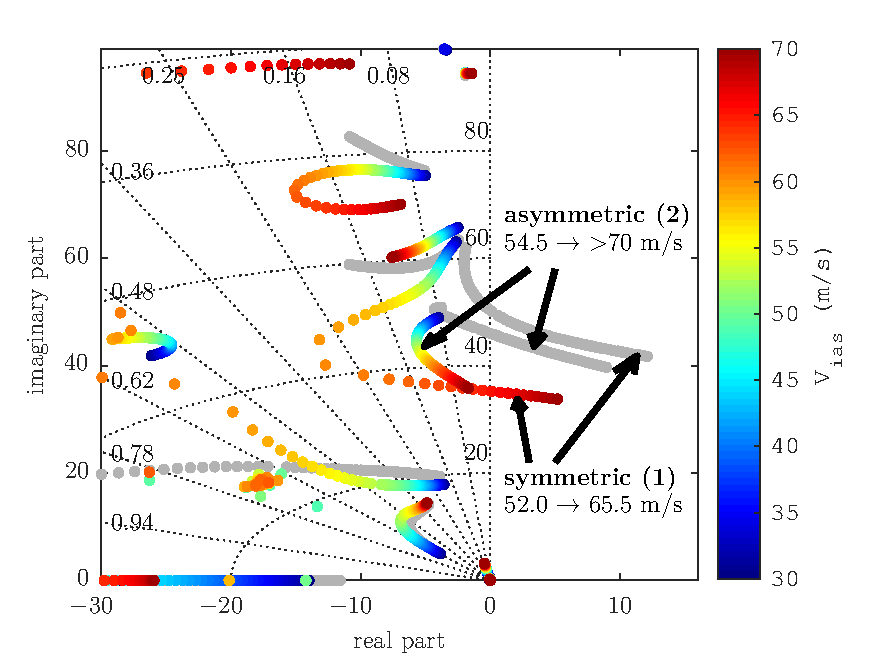
\includegraphics[width=0.7\linewidth]{figs/polesOL_CL}
%	\caption{Comparison of the open- and closed-loop poles. Only the positive part of the imaginary axis is depicted for readability reasons.}
%	\label{fig:polesx}
%\end{figure}

\begin{figure}[h]
	\centering
	% This file was created by matlab2tikz.
%
%The latest updates can be retrieved from
%  http://www.mathworks.com/matlabcentral/fileexchange/22022-matlab2tikz-matlab2tikz
%where you can also make suggestions and rate matlab2tikz.
%
\definecolor{mycolor1}{rgb}{0.00000,0.00000,0.52381}%
\definecolor{mycolor2}{rgb}{0.00000,0.00000,0.57202}%
\definecolor{mycolor3}{rgb}{0.00000,0.00000,0.62024}%
\definecolor{mycolor4}{rgb}{0.00000,0.00000,0.66845}%
\definecolor{mycolor5}{rgb}{0.00000,0.00000,0.71667}%
\definecolor{mycolor6}{rgb}{0.00000,0.00000,0.76488}%
\definecolor{mycolor7}{rgb}{0.00000,0.00000,0.81310}%
\definecolor{mycolor8}{rgb}{0.00000,0.00000,0.86131}%
\definecolor{mycolor9}{rgb}{0.00000,0.00000,0.95774}%
\definecolor{mycolor10}{rgb}{0.00000,0.00595,1.00000}%
\definecolor{mycolor11}{rgb}{0.00000,0.05417,1.00000}%
\definecolor{mycolor12}{rgb}{0.00000,0.10238,1.00000}%
\definecolor{mycolor13}{rgb}{0.00000,0.15060,1.00000}%
\definecolor{mycolor14}{rgb}{0.00000,0.19881,1.00000}%
\definecolor{mycolor15}{rgb}{0.00000,0.24702,1.00000}%
\definecolor{mycolor16}{rgb}{0.00000,0.29524,1.00000}%
\definecolor{mycolor17}{rgb}{0.00000,0.34345,1.00000}%
\definecolor{mycolor18}{rgb}{0.00000,0.39167,1.00000}%
\definecolor{mycolor19}{rgb}{0.00000,0.43988,1.00000}%
\definecolor{mycolor20}{rgb}{0.00000,0.48810,1.00000}%
\definecolor{mycolor21}{rgb}{0.00000,0.53631,1.00000}%
\definecolor{mycolor22}{rgb}{0.00000,0.58452,1.00000}%
\definecolor{mycolor23}{rgb}{0.00000,0.63274,1.00000}%
\definecolor{mycolor24}{rgb}{0.00000,0.68095,1.00000}%
\definecolor{mycolor25}{rgb}{0.00000,0.72917,1.00000}%
\definecolor{mycolor26}{rgb}{0.00000,0.77738,1.00000}%
\definecolor{mycolor27}{rgb}{0.00000,0.82560,1.00000}%
\definecolor{mycolor28}{rgb}{0.00000,0.87381,1.00000}%
\definecolor{mycolor29}{rgb}{0.00000,0.92202,1.00000}%
\definecolor{mycolor30}{rgb}{0.00000,0.97024,1.00000}%
\definecolor{mycolor31}{rgb}{0.01845,1.00000,0.98155}%
\definecolor{mycolor32}{rgb}{0.06667,1.00000,0.93333}%
\definecolor{mycolor33}{rgb}{0.11488,1.00000,0.88512}%
\definecolor{mycolor34}{rgb}{0.16310,1.00000,0.83690}%
\definecolor{mycolor35}{rgb}{0.21131,1.00000,0.78869}%
\definecolor{mycolor36}{rgb}{0.25952,1.00000,0.74048}%
\definecolor{mycolor37}{rgb}{0.30774,1.00000,0.69226}%
\definecolor{mycolor38}{rgb}{0.35595,1.00000,0.64405}%
\definecolor{mycolor39}{rgb}{0.40417,1.00000,0.59583}%
\definecolor{mycolor40}{rgb}{0.45238,1.00000,0.54762}%
\definecolor{mycolor41}{rgb}{0.50060,1.00000,0.49940}%
\definecolor{mycolor42}{rgb}{0.54881,1.00000,0.45119}%
\definecolor{mycolor43}{rgb}{0.59702,1.00000,0.40298}%
\definecolor{mycolor44}{rgb}{0.64524,1.00000,0.35476}%
\definecolor{mycolor45}{rgb}{0.74167,1.00000,0.25833}%
\definecolor{mycolor46}{rgb}{0.78988,1.00000,0.21012}%
\definecolor{mycolor47}{rgb}{0.83810,1.00000,0.16190}%
\definecolor{mycolor48}{rgb}{0.88631,1.00000,0.11369}%
\definecolor{mycolor49}{rgb}{0.93452,1.00000,0.06548}%
\definecolor{mycolor50}{rgb}{0.98274,1.00000,0.01726}%
\definecolor{mycolor51}{rgb}{1.00000,0.96905,0.00000}%
\definecolor{mycolor52}{rgb}{1.00000,0.92083,0.00000}%
\definecolor{mycolor53}{rgb}{1.00000,0.87262,0.00000}%
\definecolor{mycolor54}{rgb}{1.00000,0.82440,0.00000}%
\definecolor{mycolor55}{rgb}{1.00000,0.77619,0.00000}%
\definecolor{mycolor56}{rgb}{1.00000,0.72798,0.00000}%
\definecolor{mycolor57}{rgb}{1.00000,0.67976,0.00000}%
\definecolor{mycolor58}{rgb}{1.00000,0.63155,0.00000}%
\definecolor{mycolor59}{rgb}{1.00000,0.58333,0.00000}%
\definecolor{mycolor60}{rgb}{1.00000,0.53512,0.00000}%
\definecolor{mycolor61}{rgb}{1.00000,0.48690,0.00000}%
\definecolor{mycolor62}{rgb}{1.00000,0.43869,0.00000}%
\definecolor{mycolor63}{rgb}{1.00000,0.39048,0.00000}%
\definecolor{mycolor64}{rgb}{1.00000,0.34226,0.00000}%
\definecolor{mycolor65}{rgb}{1.00000,0.29405,0.00000}%
\definecolor{mycolor66}{rgb}{1.00000,0.24583,0.00000}%
\definecolor{mycolor67}{rgb}{1.00000,0.19762,0.00000}%
\definecolor{mycolor68}{rgb}{1.00000,0.14940,0.00000}%
\definecolor{mycolor69}{rgb}{1.00000,0.10119,0.00000}%
\definecolor{mycolor70}{rgb}{1.00000,0.05298,0.00000}%
\definecolor{mycolor71}{rgb}{0.95655,0.00000,0.00000}%
\definecolor{mycolor72}{rgb}{0.90833,0.00000,0.00000}%
\definecolor{mycolor73}{rgb}{0.86012,0.00000,0.00000}%
\definecolor{mycolor74}{rgb}{0.81190,0.00000,0.00000}%
\definecolor{mycolor75}{rgb}{0.76369,0.00000,0.00000}%
\definecolor{mycolor76}{rgb}{0.71548,0.00000,0.00000}%
\definecolor{mycolor77}{rgb}{0.66726,0.00000,0.00000}%
\definecolor{mycolor78}{rgb}{0.61905,0.00000,0.00000}%
%
\usetikzlibrary{backgrounds}

\begin{tikzpicture}[%
arrow1/.style={->,>=stealth,color=black,solid,line width=1.5pt},
arrow2/.style={->,>=stealth,color=black,solid,line width=1.5pt},
arrow3/.style={->,>=stealth,color=black,solid,line width=1.5pt},
arrow4/.style={->,>=stealth,color=black,solid,line width=1.5pt}
]

\begin{axis}[%
width=3in,
height=3in,
at={(0in,0in)},
scale only axis,
point meta min=30,
point meta max=70,
unbounded coords=jump,
xmin=-30,
xmax=16,
xlabel={Real Part},
ymin=0,
ymax=99,
ylabel={Imaginary Part},
axis background/.style={fill=white},
colormap={mymap}{[1pt] rgb(0pt)=(0,0,0.52381); rgb(9pt)=(0,0,0.957738); rgb(10pt)=(0,0.00595238,1); rgb(30pt)=(0,0.970238,1); rgb(31pt)=(0.0184524,1,0.981548); rgb(44pt)=(0.645238,1,0.354762); rgb(45pt)=(0.741667,1,0.258333); rgb(50pt)=(0.982738,1,0.0172619); rgb(51pt)=(1,0.969048,0); rgb(71pt)=(1,0.0047619,0); rgb(72pt)=(0.956548,0,0); rgb(79pt)=(0.619048,0,0)},
colorbar,
colorbar style={ylabel={$\text{V}_\text{ias}$ (m/s)}}
]
\addplot [color=white!15!black,dotted,forget plot]
  table[row sep=crcr]{%
0	0\\
-0	120\\
nan	nan\\
0	0\\
-9.6	119.61538362602\\
nan	nan\\
0	0\\
-19.2	118.454041720829\\
nan	nan\\
0	0\\
-30	116.189500386223\\
nan	nan\\
0	0\\
-43.2	111.95427638103\\
nan	nan\\
0	0\\
-57.6	105.272218557414\\
nan	nan\\
0	0\\
-74.4	94.1522171804785\\
nan	nan\\
0	0\\
-93.6	75.0935416663777\\
nan	nan\\
0	0\\
-112.8	40.9409330621567\\
nan	nan\\
0	0\\
-120	0\\
nan	nan\\
0	-0\\
-0	-120\\
nan	nan\\
0	-0\\
-9.6	-119.61538362602\\
nan	nan\\
0	-0\\
-19.2	-118.454041720829\\
nan	nan\\
0	-0\\
-30	-116.189500386223\\
nan	nan\\
0	-0\\
-43.2	-111.95427638103\\
nan	nan\\
0	-0\\
-57.6	-105.272218557414\\
nan	nan\\
0	-0\\
-74.4	-94.1522171804785\\
nan	nan\\
0	-0\\
-93.6	-75.0935416663777\\
nan	nan\\
0	-0\\
-112.8	-40.9409330621567\\
nan	nan\\
0	-0\\
-120	-0\\
nan	nan\\
};
\addplot [color=white!15!black,dotted,forget plot]
  table[row sep=crcr]{%
-0	0\\
-0	0\\
-0	0\\
-0	0\\
-0	0\\
-0	0\\
-0	0\\
-0	0\\
-0	0\\
-0	0\\
-0	0\\
-0	0\\
-0	0\\
-0	0\\
-0	0\\
-0	0\\
-0	0\\
-0	0\\
-0	0\\
-0	0\\
-0	0\\
-0	0\\
-0	0\\
-0	0\\
-0	0\\
-0	0\\
-0	0\\
-0	0\\
-0	0\\
-0	0\\
-0	0\\
-0	0\\
-0	0\\
-0	0\\
-0	0\\
-0	0\\
-0	0\\
-0	0\\
-0	0\\
-0	0\\
-0	0\\
nan	nan\\
-0	20\\
-0.365059357567957	19.996668014083\\
-0.73088087370371	19.9866408670505\\
-1.09823117266793	19.9698244431788\\
-1.46788581416878	19.9460600429399\\
-1.84063376804877	19.9151215746206\\
-2.21728188808435	19.8767115245146\\
-2.59865936824871	19.8304556046454\\
-2.98562214879027	19.7758959439175\\
-3.37905721681041	19.7124826525103\\
-3.77988671458848	19.6395635497553\\
-4.18907172583919	19.5563718024529\\
-4.60761555155734	19.4620111737982\\
-5.03656620800989	19.3554385337128\\
-5.4770177730815	19.2354432315283\\
-5.93011006488334	19.1006228856121\\
-6.397025947212	18.9493551085702\\
-6.87898530624399	18.7797646725533\\
-7.37723441500213	18.5896856451665\\
-7.89302897730223	18.3766181209565\\
-8.42760860059643	18.1376793795445\\
-8.98215976913319	17.8695496832395\\
-9.55776356609475	17.5684135770602\\
-10.1553234388745	17.229898602483\\
-10.7754672729584	16.8490149578367\\
-11.418417075695	16.4201020546609\\
-12.0838189475081	15.9367913848379\\
-12.7705262261975	15.3919998670089\\
-13.4763305314523	14.7779739953434\\
-14.1976401068741	14.0864124387894\\
-14.9291139459351	13.3087022954639\\
-15.6632754570467	12.4363098207097\\
-16.3901521226343	11.4613661226272\\
-17.0970170816858	10.3774759411209\\
-17.7683400576995	9.18074569923119\\
-18.3860773062976	7.87096952648448\\
-18.9304247850098	6.45283018985372\\
-19.3811040644749	4.93688213774603\\
-19.7191341492113	3.34002221630454\\
-19.9288786876257	1.68516890960414\\
-20	0\\
nan	nan\\
-0	40\\
-0.730118715135915	39.9933360281661\\
-1.46176174740742	39.973281734101\\
-2.19646234533586	39.9396488863575\\
-2.93577162833755	39.8921200858797\\
-3.68126753609754	39.8302431492412\\
-4.43456377616869	39.7534230490293\\
-5.19731873649742	39.6609112092909\\
-5.97124429758055	39.551791887835\\
-6.75811443362081	39.4249653050207\\
-7.55977342917695	39.2791270995106\\
-8.37814345167839	39.1127436049058\\
-9.21523110311468	38.9240223475964\\
-10.0731324160198	38.7108770674255\\
-10.954035546163	38.4708864630567\\
-11.8602201297667	38.2012457712242\\
-12.794051894424	37.8987102171404\\
-13.757970612488	37.5595293451065\\
-14.7544688300043	37.1793712903329\\
-15.7860579546045	36.753236241913\\
-16.8552172011929	36.275358759089\\
-17.9643195382664	35.739099366479\\
-19.1155271321895	35.1368271541203\\
-20.3106468777491	34.459797204966\\
-21.5509345459167	33.6980299156733\\
-22.8368341513899	32.8402041093217\\
-24.1676378950161	31.8735827696759\\
-25.5410524523951	30.7839997340177\\
-26.9526610629046	29.5559479906869\\
-28.3952802137481	28.1728248775788\\
-29.8582278918701	26.6174045909279\\
-31.3265509140933	24.8726196414193\\
-32.7803042452687	22.9227322452543\\
-34.1940341633717	20.7549518822417\\
-35.536680115399	18.3614913984624\\
-36.7721546125953	15.741939052969\\
-37.8608495700196	12.9056603797074\\
-38.7622081289497	9.87376427549207\\
-39.4382682984226	6.68004443260908\\
-39.8577573752515	3.37033781920829\\
-40	0\\
nan	nan\\
-0	60\\
-1.09517807270387	59.9900040422491\\
-2.19264262111113	59.9599226011516\\
-3.29469351800378	59.9094733295363\\
-4.40365744250633	59.8381801288196\\
-5.52190130414631	59.7453647238618\\
-6.65184566425304	59.6301345735439\\
-7.79597810474613	59.4913668139363\\
-8.95686644637082	59.3276878317525\\
-10.1371716504312	59.1374479575311\\
-11.3396601437654	58.9186906492659\\
-12.5672151775176	58.6691154073587\\
-13.822846654672	58.3860335213947\\
-15.1096986240297	58.0663156011383\\
-16.4310533192445	57.706329694585\\
-17.79033019465	57.3018686568364\\
-19.191077841636	56.8480653257107\\
-20.636955918732	56.3392940176598\\
-22.1317032450064	55.7690569354994\\
-23.6790869319067	55.1298543628695\\
-25.2828258017893	54.4130381386334\\
-26.9464793073996	53.6086490497185\\
-28.6732906982843	52.7052407311805\\
-30.4659703166236	51.689695807449\\
-32.3264018188751	50.5470448735099\\
-34.2552512270849	49.2603061639826\\
-36.2514568425242	47.8103741545138\\
-38.3115786785926	46.1759996010266\\
-40.4289915943569	44.3339219860303\\
-42.5929203206222	42.2592373163682\\
-44.7873418378052	39.9261068863918\\
-46.98982637114	37.308929462129\\
-49.170456367903	34.3840983678815\\
-51.2910512450575	31.1324278233626\\
-53.3050201730984	27.5422370976936\\
-55.1582319188929	23.6129085794534\\
-56.7912743550293	19.3584905695612\\
-58.1433121934246	14.8106464132381\\
-59.157402447634	10.0200666489136\\
-59.7866360628772	5.05550672881243\\
-60	0\\
nan	nan\\
-0	80\\
-1.46023743027183	79.9866720563322\\
-2.92352349481484	79.9465634682021\\
-4.39292469067171	79.8792977727151\\
-5.87154325667511	79.7842401717595\\
-7.36253507219509	79.6604862984824\\
-8.86912755233738	79.5068460980586\\
-10.3946374729948	79.3218224185817\\
-11.9424885951611	79.10358377567\\
-13.5162288672416	78.8499306100414\\
-15.1195468583539	78.5582541990213\\
-16.7562869033568	78.2254872098116\\
-18.4304622062294	77.8480446951929\\
-20.1462648320395	77.4217541348511\\
-21.908071092326	76.9417729261133\\
-23.7204402595334	76.4024915424485\\
-25.588103788848	75.7974204342809\\
-27.515941224976	75.119058690213\\
-29.5089376600085	74.3587425806659\\
-31.5721159092089	73.5064724838261\\
-33.7104344023857	72.5507175181779\\
-35.9286390765328	71.478198732958\\
-38.231054264379	70.2736543082406\\
-40.6212937554982	68.919594409932\\
-43.1018690918335	67.3960598313466\\
-45.6736683027798	65.6804082186434\\
-48.3352757900323	63.7471655393518\\
-51.0821049047901	61.5679994680355\\
-53.9053221258092	59.1118959813738\\
-56.7905604274963	56.3456497551576\\
-59.7164557837402	53.2348091818558\\
-62.6531018281867	49.7452392828386\\
-65.5606084905373	45.8454644905086\\
-68.3880683267434	41.5099037644835\\
-71.0733602307979	36.7229827969248\\
-73.5443092251905	31.4838781059379\\
-75.7216991400391	25.8113207594149\\
-77.5244162578995	19.7475285509841\\
-78.8765365968453	13.3600888652182\\
-79.715514750503	6.74067563841658\\
-80	0\\
nan	nan\\
-0	100\\
-1.82529678783979	99.9833400704152\\
-3.65440436851855	99.9332043352526\\
-5.49115586333964	99.8491222158939\\
-7.33942907084388	99.7303002146993\\
-9.20316884024386	99.575607873103\\
-11.0864094404217	99.3835576225732\\
-12.9932968412436	99.1522780232271\\
-14.9281107439514	98.8794797195875\\
-16.895286084052	98.5624132625518\\
-18.8994335729424	98.1978177487766\\
-20.945358629196	97.7818590122645\\
-23.0380777577867	97.3100558689911\\
-25.1828310400494	96.7771926685638\\
-27.3850888654075	96.1772161576417\\
-29.6505503244167	95.5031144280606\\
-31.98512973606	94.7467755428511\\
-34.39492653122	93.8988233627663\\
-36.8861720750106	92.9484282258323\\
-39.4651448865112	91.8830906047826\\
-42.1380430029821	90.6883968977224\\
-44.9107988456659	89.3477484161975\\
-47.7888178304738	87.8420678853008\\
-50.7766171943727	86.149493012415\\
-53.8773363647918	84.2450747891832\\
-57.0920853784748	82.1005102733043\\
-60.4190947375403	79.6839569241897\\
-63.8526311309876	76.9599993350443\\
-67.3816526572614	73.8898699767172\\
-70.9882005343703	70.432062193947\\
-74.6455697296753	66.5435114773197\\
-78.3163772852334	62.1815491035483\\
-81.9507606131716	57.3068306131358\\
-85.4850854084292	51.8873797056044\\
-88.8417002884974	45.903728496156\\
-91.9303865314881	39.3548476324224\\
-94.6521239250489	32.2641509492686\\
-96.9055203223743	24.6844106887302\\
-98.5956707460566	16.7001110815227\\
-99.6443934381287	8.42584454802072\\
-100	0\\
nan	nan\\
-0	120\\
-2.19035614540774	119.980008084498\\
-4.38528524222226	119.919845202303\\
-6.58938703600757	119.818946659073\\
-8.80731488501266	119.676360257639\\
-11.0438026082926	119.490729447724\\
-13.3036913285061	119.260269147088\\
-15.5919562094923	118.982733627873\\
-17.9137328927416	118.655375663505\\
-20.2743433008624	118.274895915062\\
-22.6793202875309	117.837381298532\\
-25.1344303550352	117.338230814717\\
-27.645693309344	116.772067042789\\
-30.2193972480593	116.132631202277\\
-32.862106638489	115.41265938917\\
-35.5806603893	114.603737313673\\
-38.382155683272	113.696130651421\\
-41.2739118374639	112.67858803532\\
-44.2634064900128	111.538113870999\\
-47.3581738638134	110.259708725739\\
-50.5656516035786	108.826076277267\\
-53.8929586147991	107.217298099437\\
-57.3465813965685	105.410481462361\\
-60.9319406332473	103.379391614898\\
-64.6528036377502	101.09408974702\\
-68.5105024541698	98.5206123279651\\
-72.5029136850484	95.6207483090277\\
-76.6231573571852	92.3519992020532\\
-80.8579831887137	88.6678439720606\\
-85.1858406412444	84.5184746327365\\
-89.5746836756103	79.8522137727837\\
-93.97965274228	74.6178589242579\\
-98.3409127358059	68.768196735763\\
-102.582102490115	62.2648556467253\\
-106.610040346197	55.0844741953871\\
-110.316463837786	47.2258171589069\\
-113.582548710059	38.7169811391223\\
-116.286624386849	29.6212928264762\\
-118.314804895268	20.0401332978272\\
-119.573272125754	10.1110134576249\\
-120	0\\
nan	nan\\
-0	-0\\
-0	-0\\
-0	-0\\
-0	-0\\
-0	-0\\
-0	-0\\
-0	-0\\
-0	-0\\
-0	-0\\
-0	-0\\
-0	-0\\
-0	-0\\
-0	-0\\
-0	-0\\
-0	-0\\
-0	-0\\
-0	-0\\
-0	-0\\
-0	-0\\
-0	-0\\
-0	-0\\
-0	-0\\
-0	-0\\
-0	-0\\
-0	-0\\
-0	-0\\
-0	-0\\
-0	-0\\
-0	-0\\
-0	-0\\
-0	-0\\
-0	-0\\
-0	-0\\
-0	-0\\
-0	-0\\
-0	-0\\
-0	-0\\
-0	-0\\
-0	-0\\
-0	-0\\
-0	-0\\
nan	nan\\
-0	-20\\
-0.365059357567957	-19.996668014083\\
-0.73088087370371	-19.9866408670505\\
-1.09823117266793	-19.9698244431788\\
-1.46788581416878	-19.9460600429399\\
-1.84063376804877	-19.9151215746206\\
-2.21728188808435	-19.8767115245146\\
-2.59865936824871	-19.8304556046454\\
-2.98562214879027	-19.7758959439175\\
-3.37905721681041	-19.7124826525103\\
-3.77988671458848	-19.6395635497553\\
-4.18907172583919	-19.5563718024529\\
-4.60761555155734	-19.4620111737982\\
-5.03656620800989	-19.3554385337128\\
-5.4770177730815	-19.2354432315283\\
-5.93011006488334	-19.1006228856121\\
-6.397025947212	-18.9493551085702\\
-6.87898530624399	-18.7797646725533\\
-7.37723441500213	-18.5896856451665\\
-7.89302897730223	-18.3766181209565\\
-8.42760860059643	-18.1376793795445\\
-8.98215976913319	-17.8695496832395\\
-9.55776356609475	-17.5684135770602\\
-10.1553234388745	-17.229898602483\\
-10.7754672729584	-16.8490149578367\\
-11.418417075695	-16.4201020546609\\
-12.0838189475081	-15.9367913848379\\
-12.7705262261975	-15.3919998670089\\
-13.4763305314523	-14.7779739953434\\
-14.1976401068741	-14.0864124387894\\
-14.9291139459351	-13.3087022954639\\
-15.6632754570467	-12.4363098207097\\
-16.3901521226343	-11.4613661226272\\
-17.0970170816858	-10.3774759411209\\
-17.7683400576995	-9.18074569923119\\
-18.3860773062976	-7.87096952648448\\
-18.9304247850098	-6.45283018985372\\
-19.3811040644749	-4.93688213774603\\
-19.7191341492113	-3.34002221630454\\
-19.9288786876257	-1.68516890960414\\
-20	-0\\
nan	nan\\
-0	-40\\
-0.730118715135915	-39.9933360281661\\
-1.46176174740742	-39.973281734101\\
-2.19646234533586	-39.9396488863575\\
-2.93577162833755	-39.8921200858797\\
-3.68126753609754	-39.8302431492412\\
-4.43456377616869	-39.7534230490293\\
-5.19731873649742	-39.6609112092909\\
-5.97124429758055	-39.551791887835\\
-6.75811443362081	-39.4249653050207\\
-7.55977342917695	-39.2791270995106\\
-8.37814345167839	-39.1127436049058\\
-9.21523110311468	-38.9240223475964\\
-10.0731324160198	-38.7108770674255\\
-10.954035546163	-38.4708864630567\\
-11.8602201297667	-38.2012457712242\\
-12.794051894424	-37.8987102171404\\
-13.757970612488	-37.5595293451065\\
-14.7544688300043	-37.1793712903329\\
-15.7860579546045	-36.753236241913\\
-16.8552172011929	-36.275358759089\\
-17.9643195382664	-35.739099366479\\
-19.1155271321895	-35.1368271541203\\
-20.3106468777491	-34.459797204966\\
-21.5509345459167	-33.6980299156733\\
-22.8368341513899	-32.8402041093217\\
-24.1676378950161	-31.8735827696759\\
-25.5410524523951	-30.7839997340177\\
-26.9526610629046	-29.5559479906869\\
-28.3952802137481	-28.1728248775788\\
-29.8582278918701	-26.6174045909279\\
-31.3265509140933	-24.8726196414193\\
-32.7803042452687	-22.9227322452543\\
-34.1940341633717	-20.7549518822417\\
-35.536680115399	-18.3614913984624\\
-36.7721546125953	-15.741939052969\\
-37.8608495700196	-12.9056603797074\\
-38.7622081289497	-9.87376427549207\\
-39.4382682984226	-6.68004443260908\\
-39.8577573752515	-3.37033781920829\\
-40	-0\\
nan	nan\\
-0	-60\\
-1.09517807270387	-59.9900040422491\\
-2.19264262111113	-59.9599226011516\\
-3.29469351800378	-59.9094733295363\\
-4.40365744250633	-59.8381801288196\\
-5.52190130414631	-59.7453647238618\\
-6.65184566425304	-59.6301345735439\\
-7.79597810474613	-59.4913668139363\\
-8.95686644637082	-59.3276878317525\\
-10.1371716504312	-59.1374479575311\\
-11.3396601437654	-58.9186906492659\\
-12.5672151775176	-58.6691154073587\\
-13.822846654672	-58.3860335213947\\
-15.1096986240297	-58.0663156011383\\
-16.4310533192445	-57.706329694585\\
-17.79033019465	-57.3018686568364\\
-19.191077841636	-56.8480653257107\\
-20.636955918732	-56.3392940176598\\
-22.1317032450064	-55.7690569354994\\
-23.6790869319067	-55.1298543628695\\
-25.2828258017893	-54.4130381386334\\
-26.9464793073996	-53.6086490497185\\
-28.6732906982843	-52.7052407311805\\
-30.4659703166236	-51.689695807449\\
-32.3264018188751	-50.5470448735099\\
-34.2552512270849	-49.2603061639826\\
-36.2514568425242	-47.8103741545138\\
-38.3115786785926	-46.1759996010266\\
-40.4289915943569	-44.3339219860303\\
-42.5929203206222	-42.2592373163682\\
-44.7873418378052	-39.9261068863918\\
-46.98982637114	-37.308929462129\\
-49.170456367903	-34.3840983678815\\
-51.2910512450575	-31.1324278233626\\
-53.3050201730984	-27.5422370976936\\
-55.1582319188929	-23.6129085794534\\
-56.7912743550293	-19.3584905695612\\
-58.1433121934246	-14.8106464132381\\
-59.157402447634	-10.0200666489136\\
-59.7866360628772	-5.05550672881243\\
-60	-0\\
nan	nan\\
-0	-80\\
-1.46023743027183	-79.9866720563322\\
-2.92352349481484	-79.9465634682021\\
-4.39292469067171	-79.8792977727151\\
-5.87154325667511	-79.7842401717595\\
-7.36253507219509	-79.6604862984824\\
-8.86912755233738	-79.5068460980586\\
-10.3946374729948	-79.3218224185817\\
-11.9424885951611	-79.10358377567\\
-13.5162288672416	-78.8499306100414\\
-15.1195468583539	-78.5582541990213\\
-16.7562869033568	-78.2254872098116\\
-18.4304622062294	-77.8480446951929\\
-20.1462648320395	-77.4217541348511\\
-21.908071092326	-76.9417729261133\\
-23.7204402595334	-76.4024915424485\\
-25.588103788848	-75.7974204342809\\
-27.515941224976	-75.119058690213\\
-29.5089376600085	-74.3587425806659\\
-31.5721159092089	-73.5064724838261\\
-33.7104344023857	-72.5507175181779\\
-35.9286390765328	-71.478198732958\\
-38.231054264379	-70.2736543082406\\
-40.6212937554982	-68.919594409932\\
-43.1018690918335	-67.3960598313466\\
-45.6736683027798	-65.6804082186434\\
-48.3352757900323	-63.7471655393518\\
-51.0821049047901	-61.5679994680355\\
-53.9053221258092	-59.1118959813738\\
-56.7905604274963	-56.3456497551576\\
-59.7164557837402	-53.2348091818558\\
-62.6531018281867	-49.7452392828386\\
-65.5606084905373	-45.8454644905086\\
-68.3880683267434	-41.5099037644835\\
-71.0733602307979	-36.7229827969248\\
-73.5443092251905	-31.4838781059379\\
-75.7216991400391	-25.8113207594149\\
-77.5244162578995	-19.7475285509841\\
-78.8765365968453	-13.3600888652182\\
-79.715514750503	-6.74067563841658\\
-80	-0\\
nan	nan\\
-0	-100\\
-1.82529678783979	-99.9833400704152\\
-3.65440436851855	-99.9332043352526\\
-5.49115586333964	-99.8491222158939\\
-7.33942907084388	-99.7303002146993\\
-9.20316884024386	-99.575607873103\\
-11.0864094404217	-99.3835576225732\\
-12.9932968412436	-99.1522780232271\\
-14.9281107439514	-98.8794797195875\\
-16.895286084052	-98.5624132625518\\
-18.8994335729424	-98.1978177487766\\
-20.945358629196	-97.7818590122645\\
-23.0380777577867	-97.3100558689911\\
-25.1828310400494	-96.7771926685638\\
-27.3850888654075	-96.1772161576417\\
-29.6505503244167	-95.5031144280606\\
-31.98512973606	-94.7467755428511\\
-34.39492653122	-93.8988233627663\\
-36.8861720750106	-92.9484282258323\\
-39.4651448865112	-91.8830906047826\\
-42.1380430029821	-90.6883968977224\\
-44.9107988456659	-89.3477484161975\\
-47.7888178304738	-87.8420678853008\\
-50.7766171943727	-86.149493012415\\
-53.8773363647918	-84.2450747891832\\
-57.0920853784748	-82.1005102733043\\
-60.4190947375403	-79.6839569241897\\
-63.8526311309876	-76.9599993350443\\
-67.3816526572614	-73.8898699767172\\
-70.9882005343703	-70.432062193947\\
-74.6455697296753	-66.5435114773197\\
-78.3163772852334	-62.1815491035483\\
-81.9507606131716	-57.3068306131358\\
-85.4850854084292	-51.8873797056044\\
-88.8417002884974	-45.903728496156\\
-91.9303865314881	-39.3548476324224\\
-94.6521239250489	-32.2641509492686\\
-96.9055203223743	-24.6844106887302\\
-98.5956707460566	-16.7001110815227\\
-99.6443934381287	-8.42584454802072\\
-100	-0\\
nan	nan\\
-0	-120\\
-2.19035614540774	-119.980008084498\\
-4.38528524222226	-119.919845202303\\
-6.58938703600757	-119.818946659073\\
-8.80731488501266	-119.676360257639\\
-11.0438026082926	-119.490729447724\\
-13.3036913285061	-119.260269147088\\
-15.5919562094923	-118.982733627873\\
-17.9137328927416	-118.655375663505\\
-20.2743433008624	-118.274895915062\\
-22.6793202875309	-117.837381298532\\
-25.1344303550352	-117.338230814717\\
-27.645693309344	-116.772067042789\\
-30.2193972480593	-116.132631202277\\
-32.862106638489	-115.41265938917\\
-35.5806603893	-114.603737313673\\
-38.382155683272	-113.696130651421\\
-41.2739118374639	-112.67858803532\\
-44.2634064900128	-111.538113870999\\
-47.3581738638134	-110.259708725739\\
-50.5656516035786	-108.826076277267\\
-53.8929586147991	-107.217298099437\\
-57.3465813965685	-105.410481462361\\
-60.9319406332473	-103.379391614898\\
-64.6528036377502	-101.09408974702\\
-68.5105024541698	-98.5206123279651\\
-72.5029136850484	-95.6207483090277\\
-76.6231573571852	-92.3519992020532\\
-80.8579831887137	-88.6678439720606\\
-85.1858406412444	-84.5184746327365\\
-89.5746836756103	-79.8522137727837\\
-93.97965274228	-74.6178589242579\\
-98.3409127358059	-68.768196735763\\
-102.582102490115	-62.2648556467253\\
-106.610040346197	-55.0844741953871\\
-110.316463837786	-47.2258171589069\\
-113.582548710059	-38.7169811391223\\
-116.286624386849	-29.6212928264762\\
-118.314804895268	-20.0401332978272\\
-119.573272125754	-10.1110134576249\\
-120	-0\\
nan	nan\\
};
\node[above left, align=right, text=black!70!darkgray]
at (axis cs:0,80) {80};
\node[above left, align=right, text=black!70!darkgray]
at (axis cs:0,60) {60};
\node[above left, align=right, text=black!70!darkgray]
at (axis cs:0,40) {40};
\node[above left, align=right, text=black!70!darkgray]
at (axis cs:0,20) {20};
\node[right, align=left, text=black!70!darkgray]
at (axis cs:-29.31,10.638) {0.94};
\node[right, align=left, text=black!70!darkgray]
at (axis cs:-29.31,23.515) {0.78};
\node[right, align=left, text=black!70!darkgray]
at (axis cs:-29.31,37.091) {0.62};
\node[right, align=left, text=black!70!darkgray]
at (axis cs:-29.31,53.568) {0.48};
\node[right, align=left, text=black!70!darkgray]
at (axis cs:-29.31,75.958) {0.36};
\node[below, align=center, text=black!70!darkgray]
at (axis cs:-25.178,97.515) {0.25};
\node[below, align=center, text=black!70!darkgray]
at (axis cs:-15.806,97.515) {0.16};
\node[below, align=center, text=black!70!darkgray]
at (axis cs:-7.826,97.515) {0.08};
\addplot [color=white!70!black,line width=1.5pt,mark size=1.5pt,only marks,mark=*,mark options={solid},forget plot]
  table[row sep=crcr]{%
-0.0314714505372846	0.429357014726761\\
-0.230876410845415	1.47693576848093\\
-4.27458443717004	5.44419070467664\\
-3.90952123349806	19.3753822242132\\
-3.77529042725068	50.9087434134854\\
-1.88866688873635	62.0691339963742\\
-2.46125480994098	63.4420962636651\\
-5.0755348379136	76.3895278615797\\
-1.91388493292252	94.5137310711714\\
-3.39783067273333	98.8307429454012\\
-0.0001	0\\
-0.0001	0\\
-0.0001	0\\
-0.0001	0\\
-0.0001	0\\
-11.5750625834049	0\\
-28.4097912681592	0\\
};
\addplot [color=white!70!black,line width=1.5pt,mark size=1.5pt,only marks,mark=*,mark options={solid},forget plot]
  table[row sep=crcr]{%
-0.0001	2.02870465729757e-07\\
-0.0001	-2.02870465729757e-07\\
-0.0310666874307334	0.421861959538791\\
-0.233567449435602	1.5000600329523\\
-4.34871483197567	5.55605105253646\\
-4.00682056816829	19.405927946469\\
-3.82506847085133	50.8992955221369\\
-1.90000764178935	61.9207214574595\\
-2.49374619044022	63.3324644089949\\
-5.14113269296294	76.4300492746891\\
-1.91422884597295	94.5102231257805\\
-3.41859867155465	98.8502385790775\\
-0.0001	0\\
-0.0001	0\\
-0.0001	0\\
-11.8672622427763	0\\
};
\addplot [color=white!70!black,line width=1.5pt,mark size=1.5pt,only marks,mark=*,mark options={solid},forget plot]
  table[row sep=crcr]{%
-0.0001	9.8781583428738e-09\\
-0.0001	-9.8781583428738e-09\\
-0.0001	3.50691789717384e-07\\
-0.0001	-3.50691789717384e-07\\
-0.0307229666289313	0.414653678286834\\
-0.236292336720686	1.52315823634213\\
-4.4228139221189	5.66912602003786\\
-4.10646467558805	19.4369174492775\\
-3.8733918672141	50.8881744013072\\
-1.91123077690195	61.7683335998084\\
-2.52719218337898	63.2208840710981\\
-5.20646928203088	76.4713445691455\\
-1.91456373473195	94.5066698954087\\
-3.43908221446259	98.8698195742647\\
-0.0001	0\\
-12.1660581965479	0\\
};
\addplot [color=white!70!black,line width=1.5pt,mark size=1.5pt,only marks,mark=*,mark options={solid},forget plot]
  table[row sep=crcr]{%
-0.0001	1.19580582925835e-08\\
-0.0001	-1.19580582925835e-08\\
-0.0304349066898128	0.407719593702942\\
-0.23904787487786	1.54622935634407\\
-4.49685521722266	5.78347870920909\\
-4.20859487782107	19.4683487796\\
-3.9201107110574	50.8752968026197\\
-1.92228976810871	61.6118498464629\\
-2.56165272533009	63.1073675535318\\
-5.27156757025237	76.5134519134823\\
-1.91488974382141	94.5030727366069\\
-3.45926920904011	98.8894922516602\\
-0.0001	0\\
-0.0001	0\\
-0.0001	0\\
-12.4717380843111	0\\
};
\addplot [color=white!70!black,line width=1.5pt,mark size=1.5pt,only marks,mark=*,mark options={solid},forget plot]
  table[row sep=crcr]{%
-0.0301970370019088	0.401043154146518\\
-0.241831090544471	1.56927241912877\\
-4.57080910986448	5.89917467606907\\
-4.31336294032542	19.5002186261662\\
-3.96506450584536	50.8605774634654\\
-1.93313077612872	61.4511463067063\\
-2.5971923913622	62.9919310640589\\
-5.33645240800565	76.5564051852918\\
-1.91520707622764	94.4994329371023\\
-3.47914955987704	98.9092632666999\\
-0.0001	0\\
-0.0001	0\\
-0.0001	0\\
-0.0001	0\\
-0.0001	0\\
-12.7846030164933	0\\
};
\addplot [color=white!70!black,line width=1.5pt,mark size=1.5pt,only marks,mark=*,mark options={solid},forget plot]
  table[row sep=crcr]{%
-0.0300046567358889	0.394610203013564\\
-0.244639275995718	1.59228650143819\\
-4.64464163775341	6.01628085739382\\
-4.42093199787515	19.5325221798498\\
-4.00808154643849	50.843928925817\\
-1.94369238486572	61.2860959333253\\
-2.63388098895188	62.8745951866225\\
-5.40114994212774	76.6002341498682\\
-1.91551598166542	94.4957517066022\\
-3.49871508016087	98.9291393477178\\
-0.0001	0\\
-0.0001	0\\
-0.0001	0\\
-0.0001	0\\
-0.0001	0\\
-13.1049709968699	0\\
};
\addplot [color=white!70!black,line width=1.5pt,mark size=1.5pt,only marks,mark=*,mark options={solid},forget plot]
  table[row sep=crcr]{%
-0.0298535739848942	0.388407583442409\\
-0.247469926244147	1.61527068979688\\
-4.71831424553969	6.13486607258547\\
-4.53147761364258	19.565253031376\\
-4.04897827865573	50.8252613370587\\
-1.95390531325704	61.1165686118887\\
-2.67179418378956	62.7553853486315\\
-5.46568713251357	76.6449646885718\\
-1.9158167431512	94.4920301861075\\
-3.51795943557817	98.9491271573768\\
-0.0001	0\\
-0.0001	0\\
-0.0001	0\\
-0.0001	0\\
-0.0001	0\\
-13.4331718874152	0\\
};
\addplot [color=white!70!black,line width=1.5pt,mark size=1.5pt,only marks,mark=*,mark options={solid},forget plot]
  table[row sep=crcr]{%
-0.0001	7.12522719830046e-09\\
-0.0001	-7.12522719830046e-09\\
-0.0001	8.13736976636113e-08\\
-0.0001	-8.13736976636113e-08\\
-0.0297400446413101	0.382423059936674\\
-0.250320762523121	1.63822413546247\\
-4.79178327208112	6.25500121686169\\
-4.64518895489114	19.5984030420264\\
-4.08755860958016	50.8044822190966\\
-1.96369208248753	60.9424312354078\\
-2.71101414121382	62.6343323339826\\
-5.53009132293997	76.6906190560686\\
-1.91610966671697	94.4882694446303\\
-3.53687780993466	98.9692330769326\\
-0.0001	0\\
-13.7695572568733	0\\
};
\addplot [color=white!70!black,line width=1.5pt,mark size=1.5pt,only marks,mark=*,mark options={solid},forget plot]
  table[row sep=crcr]{%
-0.0296607174844581	0.376645231095517\\
-0.253189663254156	1.66114598693899\\
-4.86499939928027	6.37675944044083\\
-4.76227010343369	19.6319622208893\\
-4.12361320664325	50.7814962076815\\
-1.97296663228005	60.7635477650444\\
-2.75163017673221	62.511472838872\\
-5.59438988866336	76.7372161462138\\
-1.91639507317493	94.4844704833989\\
-3.55546709278689	98.9894630448874\\
-0.0001	0\\
-0.0001	0\\
-0.0001	0\\
-0.0001	0\\
-0.0001	0\\
-14.1144912629408	0\\
};
\addplot [color=white!70!black,line width=1.5pt,mark size=1.5pt,only marks,mark=*,mark options={solid},forget plot]
  table[row sep=crcr]{%
-0.0001	4.61016354074341e-08\\
-0.0001	-4.61016354074341e-08\\
-0.029612589940751	0.37106348102006\\
-0.256074682975546	1.68403543221917\\
-4.93790698104328	6.50021626865541\\
-4.88294151301011	19.6659185896439\\
-4.15691876438206	50.7562047500443\\
-1.98163387957963	60.579779281615\\
-2.7937394105964	62.3868500947392\\
-5.65860993567692	76.784771777351\\
-1.91667328790934	94.4806342397744\\
-3.57372536502008	99.0098224323615\\
-0.0001	0\\
-0.0001	0\\
-0.0001	0\\
-14.4683587076641	0\\
};
\addplot [color=white!70!black,line width=1.5pt,mark size=1.5pt,only marks,mark=*,mark options={solid},forget plot]
  table[row sep=crcr]{%
-0.0001	9.22629212817507e-09\\
-0.0001	-9.22629212817507e-09\\
-0.0001	3.89118512169895e-08\\
-0.0001	-3.89118512169895e-08\\
-0.0295929583588446	0.365667829456053\\
-0.258974038959088	1.70689169952684\\
-5.01044328317255	6.62544971025067\\
-5.00744163949628	19.7002580505169\\
-4.18723728051154	50.7285057562905\\
-1.98958921025923	60.3909840358592\\
-2.837447412593	62.2605145651106\\
-5.72277806014661	76.8332989742049\\
-1.91694462934601	94.4767615894369\\
-3.59165192159782	99.0303161393669\\
-0.0001	0\\
-14.8315667858659	0\\
};
\addplot [color=white!70!black,line width=1.5pt,mark size=1.5pt,only marks,mark=*,mark options={solid},forget plot]
  table[row sep=crcr]{%
-0.0001	1.46689666775468e-09\\
-0.0001	-1.46689666775468e-09\\
-0.0295993958357686	0.360448993690643\\
-0.261886058901313	1.72971400690625\\
-5.08253765433702	6.75254029838722\\
-5.1360287642416	19.73496427737\\
-4.21431534613146	50.6982931800859\\
-1.99671789831925	60.1970175062556\\
-2.88286882179621	62.1325247404945\\
-5.78692015297855	76.8828082289079\\
-1.91720941174246	94.4728533542921\\
-3.60924728364802	99.0509481874469\\
-0.0001	0\\
-0.0001	0\\
-0.0001	0\\
-15.2045377011222	0\\
};
\addplot [color=white!70!black,line width=1.5pt,mark size=1.5pt,only marks,mark=*,mark options={solid},forget plot]
  table[row sep=crcr]{%
-0.0001	1.48477945375491e-08\\
-0.0001	-1.48477945375491e-08\\
-0.0296297190974112	0.355398322685496\\
-0.264809208131274	1.7525016080238\\
-5.15411051728964	6.88157104446579\\
-5.26898302018096	19.7700185949496\\
-4.23788346686345	50.6654565350644\\
-2.00289444212833	59.9977324724921\\
-2.93012793023858	62.0029480462757\\
-5.85106125022532	76.9333077814754\\
-1.91746793271336	94.468910305118\\
-3.62651271207691	99.0717219717344\\
-0.0001	0\\
-0.0001	0\\
-0.0001	0\\
-15.5877179309691	0\\
};
\addplot [color=white!70!black,line width=1.5pt,mark size=1.5pt,only marks,mark=*,mark options={solid},forget plot]
  table[row sep=crcr]{%
-0.0001	3.06383561793125e-09\\
-0.0001	-3.06383561793125e-09\\
-0.0296819515484428	0.350507647047842\\
-0.267742074136224	1.77525378744078\\
-5.22507225285395	7.01262733242659\\
-5.40660866447659	19.805399899196\\
-4.25765545967378	50.6298803121499\\
-2.00798181048537	59.792979114892\\
-2.97935919980671	61.8718618867121\\
-5.91522541950485	76.9848038719572\\
-1.91772046742593	94.464933169933\\
-3.64345038451969	99.0926402400885\\
-0.0001	0\\
-0.0001	0\\
-0.0001	0\\
-15.9815790961724	0\\
};
\addplot [color=white!70!black,line width=1.5pt,mark size=1.5pt,only marks,mark=*,mark options={solid},forget plot]
  table[row sep=crcr]{%
-0.0297543086798479	0.345769324765114\\
-0.270683341393789	1.79796983870224\\
-5.29532195312924	7.14579670201054\\
-5.54923661589831	19.8410846222193\\
-4.27332794554591	50.5914432849844\\
-2.01183059030254	59.5826051527292\\
-3.03070768690443	61.739354849106\\
-5.97943567402046	77.037300974621\\
-1.91796727129352	94.460922635475\\
-3.66006317691803	99.1137048979128\\
-0.0001	0\\
-0.0001	0\\
-0.0001	0\\
-0.0001	0\\
-0.0001	0\\
-16.3866156789637	0\\
};
\addplot [color=white!70!black,line width=1.5pt,mark size=1.5pt,only marks,mark=*,mark options={solid},forget plot]
  table[row sep=crcr]{%
-0.0001	1.48547943208967e-08\\
-0.0001	-1.48547943208967e-08\\
-0.0001	1.48548245286576e-08\\
-0.0001	-1.48548245286576e-08\\
-0.0298451752163485	0.341176181412299\\
-0.27363177359408	1.82064905381711\\
-5.36474596575518	7.28116845619114\\
-5.69722727953457	19.8770467415562\\
-4.2845799894705	50.5500176873581\\
-2.01427802567129	59.366456035915\\
-3.08432933762711	61.6055280906959\\
-6.0437139228023	77.0908020288415\\
-1.9182085733221	94.4568793565218\\
-3.67635443676132	99.1349170334139\\
-0.0001	0\\
-16.8033429129757	0\\
};
\addplot [color=white!70!black,line width=1.5pt,mark size=1.5pt,only marks,mark=*,mark options={solid},forget plot]
  table[row sep=crcr]{%
-0.0299530863693539	0.336721467897939\\
-0.276586231197479	1.84329075384378\\
-5.43321629513921	7.41883312910617\\
-5.85097370570976	19.9132578929441\\
-4.29107294773758	50.5054682465643\\
-2.01514693874681	59.1443752053032\\
-3.14039110442631	61.4704969276116\\
-6.10808092974304	77.1453086461257\\
-1.91844457401091	94.4528039540419\\
-3.69232802184248	99.1562770532005\\
-0.0001	0\\
-0.0001	0\\
-0.0001	0\\
-0.0001	0\\
-0.0001	0\\
-17.23230505112	0\\
};
\addplot [color=white!70!black,line width=1.5pt,mark size=1.5pt,only marks,mark=*,mark options={solid},forget plot]
  table[row sep=crcr]{%
-0.0001	1.4389577401944e-08\\
-0.0001	-1.4389577401944e-08\\
-0.0001	3.46446174451554e-08\\
-0.0001	-3.46446174451554e-08\\
-0.0300767128297897	0.332398839789752\\
-0.279545678270647	1.86589430121819\\
-5.50058873832744	7.55888163714707\\
-6.010905078275	19.9496875737931\\
-4.29245058537612	50.4576510473111\\
-2.01424452492918	58.9162044433489\\
-3.19907082356414	61.3343926503333\\
-6.17255632006709	77.2008213042664\\
-3.70798833083202	99.1777848165527\\
-1.91867544596048	94.4486970333887\\
-0.0001	0\\
-17.6740817233092	0\\
};
\addplot [color=white!70!black,line width=1.5pt,mark size=1.5pt,only marks,mark=*,mark options={solid},forget plot]
  table[row sep=crcr]{%
-0.0001	5.22001833173275e-08\\
-0.0001	-5.22001833173275e-08\\
-0.0302148461371225	0.328202322260158\\
-0.282509106792404	1.88845902187144\\
-5.5667009168452	7.70140422800315\\
-6.17749061007817	19.9863035511333\\
-4.28833954333252	50.4064122139018\\
-2.01136100923386	58.6817843359894\\
-3.26055678386145	61.1973645806531\\
-6.23715856099355	77.2573395234038\\
-1.91890133087239	94.4445591729323\\
-3.723339770075	99.199439243511\\
-0.0001	0\\
-0.0001	0\\
-0.0001	0\\
-18.1292678170474	0\\
};
\addplot [color=white!70!black,line width=1.5pt,mark size=1.5pt,only marks,mark=*,mark options={solid},forget plot]
  table[row sep=crcr]{%
-0.0001	3.04707645026606e-08\\
-0.0001	-3.04707645026606e-08\\
-0.0303663860746538	0.324126281336569\\
-0.285475605010555	1.9109842885055\\
-5.6313699781819	7.84648892554689\\
-6.35124380279761	20.0230724528281\\
-4.27835027877411	50.3515864245307\\
-2.00626815797551	58.4409548768486\\
-3.32504688818309	61.0595823640433\\
-6.30190499691326	77.3148620262419\\
-1.919122341864	94.4403909410592\\
-3.73838716602447	99.2212387721733\\
-0.0001	0\\
-0.0001	0\\
-0.0001	0\\
-18.5984977258385	0\\
};
\addplot [color=white!70!black,line width=1.5pt,mark size=1.5pt,only marks,mark=*,mark options={solid},forget plot]
  table[row sep=crcr]{%
-0.0001	1.62642941165481e-08\\
-0.0001	-1.62642941165481e-08\\
-0.030530329969554	0.320165403710221\\
-0.288444314326368	1.93346947768325\\
-5.69439017706791	7.99421954561979\\
-6.53272712277616	20.0599606732568\\
-4.26207857351503	50.2929952512427\\
-1.99871763541278	58.1935562442004\\
-3.39274730750704	60.9212384944841\\
-6.36681186780446	77.3733868835774\\
-1.91933856244776	94.436192895167\\
-3.75313545478243	99.2431811970329\\
-0.0001	0\\
-0.0001	0\\
-0.0001	0\\
-19.0824350330528	0\\
};
\addplot [color=white!70!black,line width=1.5pt,mark size=1.5pt,only marks,mark=*,mark options={solid},forget plot]
  table[row sep=crcr]{%
-0.0307057626381727	0.316314670887639\\
-0.291414432903263	1.9559139783931\\
-5.755530239044	8.14467303922224\\
-6.7225570563346	20.0969356614539\\
-4.23910777014073	50.2304453768038\\
-1.98843919904073	57.9394297931416\\
-3.46387049626707	60.7825510246266\\
-6.43189434713857	77.4329116449927\\
-1.91955004763739	94.4319655858974\\
-3.76758966300835	99.2652637464591\\
-0.0001	0\\
-0.0001	0\\
-0.0001	0\\
-0.0001	0\\
-0.0001	0\\
-19.581776539146	0\\
};
\addplot [color=white!70!black,line width=1.5pt,mark size=1.5pt,only marks,mark=*,mark options={solid},forget plot]
  table[row sep=crcr]{%
-0.0001	3.1939089571195e-09\\
-0.0001	-3.1939089571195e-09\\
-0.0001	8.60172992858118e-07\\
-0.0001	-8.60172992858118e-07\\
-0.0308918480343719	0.312569343138252\\
-0.294385211652966	1.97831719221594\\
-5.8145306373651	8.29791605070222\\
-6.92140949356622	20.1339677026449\\
-4.2090118836824	50.1637267563394\\
-1.97513873025985	57.6784193088451\\
-3.53863242927256	60.6437663870502\\
-6.49716658161799	77.49343345568\\
-1.91975682587223	94.4277095602186\\
-3.78175491259327	99.2874831530034\\
-0.0001	0\\
-20.0972537965305	0\\
};
\addplot [color=white!70!black,line width=1.5pt,mark size=1.5pt,only marks,mark=*,mark options={solid},forget plot]
  table[row sep=crcr]{%
-0.0001	1.70814344689557e-08\\
-0.0001	-1.70814344689557e-08\\
-0.0001	5.91840195049089e-07\\
-0.0001	-5.91840195049089e-07\\
-0.0310878211442214	0.308924935521372\\
-0.297355947177697	2.00067852964267\\
-5.87110082897923	8.45400047573954\\
-7.13002535324323	20.1710323263935\\
-4.17135975628594	50.0926108431199\\
-1.95849610086574	57.4103725790142\\
-3.61724891040551	60.5051621999294\\
-6.56264174029906	77.5549491613971\\
-1.91995889896137	94.4234253667683\\
-3.79563627652567	99.3098356360999\\
-0.0001	0\\
-20.6296336026939	0\\
};
\addplot [color=white!70!black,line width=1.5pt,mark size=1.5pt,only marks,mark=*,mark options={solid},forget plot]
  table[row sep=crcr]{%
-0.0001	1.39222538997929e-08\\
-0.0001	-1.39222538997929e-08\\
-0.0312929813498437	0.305377203952268\\
-0.300325981680834	2.0229974134986\\
-5.92491670472688	8.61295782494094\\
-7.34921625770007	20.2081134915061\\
-4.12572042241211	50.0168490624768\\
-1.93816288242466	57.1351433513948\\
-3.69993080533597	60.3670498665206\\
-6.62833206070743	77.61745539978\\
-1.92015624525183	94.4191135562485\\
-3.80923884540961	99.3323170110236\\
-0.0001	0\\
-0.0001	0\\
-0.0001	0\\
-21.1797206984959	0\\
};
\addplot [color=white!70!black,line width=1.5pt,mark size=1.5pt,only marks,mark=*,mark options={solid},forget plot]
  table[row sep=crcr]{%
-0.0315066862253165	0.301922128423884\\
-0.30329469709495	2.04527327599016\\
-5.97561845338021	8.77479213270206\\
-7.57986999346819	20.2452076924327\\
-4.07166981770013	49.9361717859893\\
-1.9137599160863	56.8525937564185\\
-3.7868780775755	60.2297766993098\\
-6.6942489018921	77.6809486818727\\
-1.92034882075989	94.4147746853928\\
-3.82256764418305	99.3549227056005\\
-0.0001	0\\
-0.0001	0\\
-0.0001	0\\
-0.0001	0\\
-0.0001	0\\
-21.7483585024813	0\\
};
\addplot [color=white!70!black,line width=1.5pt,mark size=1.5pt,only marks,mark=*,mark options={solid},forget plot]
  table[row sep=crcr]{%
-0.0001	1.99693661375931e-08\\
-0.0001	-1.99693661375931e-08\\
-0.031728346043432	0.298555898273414\\
-0.306261516180544	2.0675055624019\\
-6.02280929904248	8.93947121065994\\
-7.82295532563492	20.2823291220425\\
-4.00879892050718	49.8502881468635\\
-1.88487477271778	56.5625972860686\\
-3.87827256101167	60.093727214002\\
-6.76040279445654	77.7454254644686\\
-1.92053656177384	94.4104093172176\\
-3.83562763916229	99.3776477823228\\
-0.0001	0\\
-0.0001	0\\
-0.0001	0\\
-22.3364326776202	0\\
};
\addplot [color=white!70!black,line width=1.5pt,mark size=1.5pt,only marks,mark=*,mark options={solid},forget plot]
  table[row sep=crcr]{%
-0.0001	1.48353008237553e-08\\
-0.0001	-1.48353008237553e-08\\
-0.0001	7.43180196263068e-07\\
-0.0001	-7.43180196263068e-07\\
-0.0319574188682362	0.295274898630734\\
-0.30922589123227	2.08969372239615\\
-6.0660556448094	9.10691602154614\\
-8.07952556707263	20.3195159536649\\
-3.93672330859948	49.7588871188304\\
-1.85105915371075	56.2650424356348\\
-3.97426949947042	59.9593231500557\\
-6.82680349676984	77.8108822100633\\
-1.92071938572771	94.4060180265048\\
-3.84842367512398	99.4004870344884\\
-0.0001	0\\
-22.9448687895072	0\\
};
\addplot [color=white!70!black,line width=1.5pt,mark size=1.5pt,only marks,mark=*,mark options={solid},forget plot]
  table[row sep=crcr]{%
-0.0321934061609922	0.29207569796338\\
-0.312187310510514	2.11183721879303\\
-6.1048894422223	9.27698818107085\\
-8.35072005045246	20.3568376792545\\
-3.85509396548587	49.661640336552\\
-1.81182630663713	55.9598371272264\\
-4.07498803440287	59.8270217101315\\
-6.89346004349865	77.8773154428438\\
-1.92089719536592	94.4016013974147\\
-3.86096049912776	99.4234349793813\\
-0.0001	0\\
-0.0001	0\\
-0.0001	0\\
-0.0001	0\\
-0.0001	0\\
-23.5746393031575	0\\
};
\addplot [color=white!70!black,line width=1.5pt,mark size=1.5pt,only marks,mark=*,mark options={solid},forget plot]
  table[row sep=crcr]{%
-0.0324358488225093	0.288955036434387\\
-0.315145293406119	2.13393552451394\\
-6.13881377678207	9.44947570101614\\
-8.63776242628854	20.3944031863682\\
-3.7636089686172	49.5582071649428\\
-1.76664856592068	55.6469140476578\\
-4.18050102096576	59.6973114861037\\
-6.96038079671204	77.9447217957782\\
-1.92106987963187	94.3971600249734\\
-3.8732427673031	99.4464858912092\\
-0.0001	0\\
-0.0001	0\\
-0.0001	0\\
-0.0001	0\\
-0.0001	0\\
-24.2267648546852	0\\
};
\addplot [color=white!70!black,line width=1.5pt,mark size=1.5pt,only marks,mark=*,mark options={solid},forget plot]
  table[row sep=crcr]{%
-0.0326843236567632	0.285909815227396\\
-0.318099385240363	2.15598811948644\\
-6.16731285837741	9.62407754372923\\
-8.94195445174095	20.4323688511488\\
-3.66202543850028	49.4482424508609\\
-1.71495517224979	55.3262370413228\\
-4.29082479877226	59.5707055965137\\
-7.02757349862248	78.0130980464122\\
-1.92123731590934	94.3926945205588\\
-3.88527495339235	99.4696338779614\\
-0.0001	0\\
-0.0001	0\\
-0.0001	0\\
-0.0001	0\\
-0.0001	0\\
-24.9023152136434	0\\
};
\addplot [color=white!70!black,line width=1.5pt,mark size=1.5pt,only marks,mark=*,mark options={solid},forget plot]
  table[row sep=crcr]{%
-0.0001	1.69763290581718e-08\\
-0.0001	-1.69763290581718e-08\\
-0.0001	1.19145251221301e-06\\
-0.0001	-1.19145251221301e-06\\
-0.0329384401825182	0.282937086682668\\
-0.321049156604421	2.17799449186605\\
-6.1898677324927	9.8003882062315\\
-9.2646637857302	20.4709453416732\\
-3.55017087532641	49.3314072244699\\
-1.65613058298836	54.9978086997201\\
-4.40590979668696	59.4477317330648\\
-7.09504531702906	78.0824411549216\\
-1.92139937307596	94.3882055062977\\
-3.89706143941556	99.4928729010584\\
-0.0001	0\\
-25.6024148777762	0\\
};
\addplot [color=white!70!black,line width=1.5pt,mark size=1.5pt,only marks,mark=*,mark options={solid},forget plot]
  table[row sep=crcr]{%
-0.0001	6.97348574362559e-07\\
-0.0001	-6.97348574362559e-07\\
-0.0331978377443624	0.280034044898088\\
-0.323994203631392	2.19995413949038\\
-6.20597883166588	9.97788418859011\\
-9.60730444611441	20.5104010479092\\
-3.42795278167702	49.207382309291\\
-1.58951355665854	54.6616792794651\\
-4.52563306521184	59.3289191095949\\
-7.16280289200272	78.152748290743\\
-1.9215559132829	94.3836936195365\\
-3.90860645886727	99.5161967823281\\
-0.0001	0\\
-0.0001	0\\
-0.0001	0\\
-26.3282474267961	0\\
};
\addplot [color=white!70!black,line width=1.5pt,mark size=1.5pt,only marks,mark=*,mark options={solid},forget plot]
  table[row sep=crcr]{%
-0.0001	1.27041065999867e-08\\
-0.0001	-1.27041065999867e-08\\
-0.0334621829457946	0.277198017493416\\
-0.326934143893635	2.22186656758604\\
-6.21519589511611	10.1559152491017\\
-9.97130904234809	20.5510591622082\\
-3.29536537795181	49.0758843657393\\
-1.51439738243407	54.3179570480006\\
-4.64979391802295	59.2147827426271\\
-7.23085238080162	78.2240168559463\\
-1.92170679402929	94.3791595114855\\
-3.91991411626727	99.5395992621849\\
-0.0001	0\\
-0.0001	0\\
-0.0001	0\\
-27.0810617528702	0\\
};
\addplot [color=white!70!black,line width=1.5pt,mark size=1.5pt,only marks,mark=*,mark options={solid},forget plot]
  table[row sep=crcr]{%
-0.0337311672888513	0.274426457415284\\
-0.329868610656268	2.24373128385337\\
-6.21715460200069	10.333704072159\\
-10.3580930539761	20.5932847389735\\
-3.15249230158415	48.9366833948896\\
-1.43003172430465	53.9668200976621\\
-4.77811376862601	59.1058059880339\\
-7.29919950125013	78.2962445048649\\
-1.92185187040578	94.3746038499114\\
-3.93098841539584	99.5630740497146\\
-0.0001	0\\
-0.0001	0\\
-0.0001	0\\
-0.0001	0\\
-0.0001	0\\
-27.8621611350999	0\\
};
\addplot [color=white!70!black,line width=1.5pt,mark size=1.5pt,only marks,mark=*,mark options={solid},forget plot]
  table[row sep=crcr]{%
-0.0001	7.43950087219644e-09\\
-0.0001	-7.43950087219644e-09\\
-0.0340045050696973	0.271716935634105\\
-0.332797287917265	2.26554783533069\\
-6.2116173662658	10.5103581649208\\
-10.7690132198204	20.6374578016251\\
-1.33562665912826	53.6085295651506\\
-2.99950451372093	48.7896202470082\\
-4.91024090721131	59.00242274443\\
-7.36784956248445	78.3694291618729\\
-1.92199099788921	94.3700273082293\\
-3.94183305096753	99.5866146439734\\
-0.0001	0\\
-0.0001	0\\
-0.0001	0\\
-28.6730217726569	0\\
};
\addplot [color=white!70!black,line width=1.5pt,mark size=1.5pt,only marks,mark=*,mark options={solid},forget plot]
  table[row sep=crcr]{%
-0.0342819314711298	0.269067134519301\\
-0.335719825600982	2.28731572484941\\
-6.19851350218778	10.6848973436616\\
-11.2053241062685	20.6839297521143\\
-1.2303595904747	53.2434440364684\\
-2.83665320437818	48.6346223800556\\
-5.0457603685187	58.9050010217146\\
-7.43680752148226	78.4435690289098\\
-1.92212403275428	94.3654305859239\\
-3.95245188498663	99.61021481474\\
-0.0001	0\\
-0.0001	0\\
-0.0001	0\\
-0.0001	0\\
-0.0001	0\\
-29.5150832681974	0\\
};
\addplot [color=white!70!black,line width=1.5pt,mark size=1.5pt,only marks,mark=*,mark options={solid},forget plot]
  table[row sep=crcr]{%
-0.0001	1.18239286806463e-08\\
-0.0001	-1.18239286806463e-08\\
-0.0001	1.18241602846517e-08\\
-0.0001	-1.18241602846517e-08\\
-0.034563200810102	0.266474840959352\\
-0.338635926324489	2.30903450349759\\
-6.17797182249891	10.8562973054336\\
-13.3352537511132	13.7756517840012\\
-11.6681395217343	20.7329623211345\\
-16.9888382340009	17.7475818902457\\
-2.66425817566852	48.4717160552815\\
-1.11338580309934	52.8720346895131\\
-5.18420838232217	58.8138296602137\\
-7.50607800515088	78.5186625985104\\
-1.92225083510962	94.3608143881646\\
-3.96284843217087	99.6338681096229\\
-0.0001	0\\
};
\addplot [color=white!70!black,line width=1.5pt,mark size=1.5pt,only marks,mark=*,mark options={solid},forget plot]
  table[row sep=crcr]{%
-0.0348480849845969	0.263937940852581\\
-0.341545560797759	2.3307044370676\\
-6.15033584256716	11.0235461404316\\
-12.1584042686395	20.784654498501\\
-18.8085575610385	17.2806656664305\\
-26.2671828282946	18.6288437727353\\
-2.48269192567986	48.3010349175212\\
-0.983853968486165	52.4949006933369\\
-5.32509802357186	58.7291094740237\\
-7.57566451408488	78.5947090879729\\
-1.9223716653627	94.356179858656\\
-3.97302544894128	99.6575711481754\\
-0.0001	0\\
-0.0001	0\\
-0.0001	0\\
-0.0001	0\\
-0.0001	0\\
};
\addplot [color=white!70!black,line width=1.5pt,mark size=1.5pt,only marks,mark=*,mark options={solid},forget plot]
  table[row sep=crcr]{%
-0.0001	1.23714002962187e-08\\
-0.0001	-1.23714002962187e-08\\
-0.0351363720262599	0.261454413072869\\
-0.344447692880069	2.35232289910108\\
-6.11617034063747	11.1857110486769\\
-12.6768877773514	20.8388542590287\\
-16.1167422823741	19.8142261375946\\
-2.29236780756132	48.1228142200719\\
-0.840923611078307	52.1127818234042\\
-5.46789892415004	58.6509509039095\\
-7.64557357461619	78.6717063334807\\
-1.92248520579769	94.3515264370958\\
-3.98298849165812	99.6813087676191\\
-0.0001	0\\
-0.0001	0\\
-0.0001	0\\
};
\addplot [color=white!70!black,line width=1.5pt,mark size=1.5pt,only marks,mark=*,mark options={solid},forget plot]
  table[row sep=crcr]{%
-0.035427864821295	0.259022324870682\\
-0.347342816596715	2.37389162899745\\
-6.07621244014111	11.3419927538988\\
-13.2241865228345	20.8950988974161\\
-2.09371395664212	47.9374001133808\\
-0.683796151892409	51.7265724393003\\
-5.61213553009191	58.5793744616122\\
-7.71580656110358	78.7496549903587\\
-1.92259252874314	94.3468561571923\\
-3.99273860258817	99.7050835744087\\
-0.0001	0\\
-0.0001	0\\
-0.0001	0\\
-0.0001	0\\
-0.0001	0\\
-14.2148400272157	0\\
};
\addplot [color=white!70!black,line width=1.5pt,mark size=1.5pt,only marks,mark=*,mark options={solid},forget plot]
  table[row sep=crcr]{%
-0.0001	1.17237086696982e-08\\
-0.0001	-1.17237086696982e-08\\
-0.0357223799177503	0.256639826556694\\
-0.35023036803395	2.39540927297129\\
-6.03134363863456	11.491782592274\\
-17.6952617464006	15.677489553805\\
-13.8008254695302	20.9526800325797\\
-17.875790605989	17.7432418793241\\
-1.88716798752844	47.745225535397\\
-0.511741057235689	51.3373249038106\\
-5.75732230408268	58.514323180039\\
-7.78636267177848	78.8285571216829\\
-1.92269245595858	94.3421688629498\\
-4.00228100967546	99.7288863364556\\
-0.0001	0\\
-0.0001	0\\
-0.0001	0\\
};
\addplot [color=white!70!black,line width=1.5pt,mark size=1.5pt,only marks,mark=*,mark options={solid},forget plot]
  table[row sep=crcr]{%
-0.0001	7.43498397842172e-09\\
-0.0001	-7.43498397842172e-09\\
-0.0360197464546558	0.254305147118017\\
-0.353110326852472	2.4168760077149\\
-5.98252401977545	11.634661436418\\
-14.4069460506425	21.0099406198787\\
-1.67316161241561	47.5468031397792\\
-0.32413432808415	50.9462524016493\\
-5.90302866872735	58.4556555660366\\
-7.85726108492527	78.9084044325057\\
-1.92278690393588	94.337466734615\\
-4.01161476656238	99.7527112811916\\
-0.0001	0\\
-0.0001	0\\
-0.0001	0\\
};
\addplot [color=white!70!black,line width=1.5pt,mark size=1.5pt,only marks,mark=*,mark options={solid},forget plot]
  table[row sep=crcr]{%
-0.036319805182033	0.252016589971617\\
-0.35598225095406	2.43829080279679\\
-5.93072089045858	11.7704489588186\\
-15.043027084111	21.0656378387205\\
-1.45211126829892	47.3427070207054\\
-0.120498610791945	50.5547148310929\\
-6.04885707531509	58.4031927495614\\
-7.92848934918343	78.9892055591743\\
-1.92287377033981	94.3327491136011\\
-4.02074687517438	99.7765520977272\\
-0.0001	0\\
-0.0001	0\\
-0.0001	0\\
-0.0001	0\\
-0.0001	0\\
};
\addplot [color=white!70!black,line width=1.5pt,mark size=1.5pt,only marks,mark=*,mark options={solid},forget plot]
  table[row sep=crcr]{%
-0.0366224075553735	0.249772528979134\\
-0.358846007916429	2.4596534542238\\
-5.87686537624551	11.89913839681\\
-15.7092319766657	21.1176167427312\\
-1.22441572372845	47.133555139035\\
0.0994575926154155	50.1642013233526\\
-6.19447191591969	58.3566983993776\\
-8.00005585717153	79.0709583628116\\
-1.92295365290729	94.3280172431205\\
-4.02967886757946	99.8004030018483\\
-0.0001	0\\
-0.0001	0\\
-0.0001	0\\
-0.0001	0\\
-0.0001	0\\
};
\addplot [color=white!70!black,line width=1.5pt,mark size=1.5pt,only marks,mark=*,mark options={solid},forget plot]
  table[row sep=crcr]{%
-0.0001	1.91685032750501e-08\\
-0.0001	-1.91685032750501e-08\\
-0.0001	5.79347335946045e-06\\
-0.0001	-5.79347335946045e-06\\
-0.0372346978198823	0.245411720808322\\
-0.364548219893467	2.50222070523306\\
-5.76628396059715	12.1359753057223\\
-17.1328639624212	21.2008810029846\\
-0.750583627926559	46.7026714409935\\
0.588352140692448	49.3926237296102\\
-6.48397937859761	58.2805425300942\\
-8.14421562293912	79.2373230452758\\
-1.92309225294271	94.3185138578307\\
-4.04695384402267	99.8481121495709\\
-0.0001	0\\
};
\addplot [color=white!70!black,line width=1.5pt,mark size=1.5pt,only marks,mark=*,mark options={solid},forget plot]
  table[row sep=crcr]{%
-0.0001	3.13002386439614e-09\\
-0.0001	-3.13002386439614e-09\\
-0.0001	6.02974181844898e-09\\
-0.0001	-6.02974181844898e-09\\
-0.0375441352597995	0.243292040911949\\
-0.367385954359619	2.52342593981777\\
-5.7107585980853	12.2446540555712\\
-17.5902498920278	17.9108177779673\\
-17.599467810595	17.9586388738952\\
-18.3470780466445	18.4375197804231\\
-17.8618230499539	19.7303643499454\\
-17.8884528843224	21.2361978853115\\
-0.505145796993279	46.4822408181767\\
0.856653771272161	49.0148109177832\\
-6.62737045542933	58.2502405873761\\
-8.21680605990269	79.3219510919208\\
-1.92317938496905	94.3137586896573\\
-4.0548509643365	99.8719586422678\\
-0.0001	0\\
};
\addplot [color=white!70!black,line width=1.5pt,mark size=1.5pt,only marks,mark=*,mark options={solid},forget plot]
  table[row sep=crcr]{%
-0.0001	1.22304935946061e-08\\
-0.0001	-1.22304935946061e-08\\
-0.0378556138138295	0.241210985809854\\
-0.370215477223755	2.54457459809783\\
-5.65623601877208	12.3476610861674\\
-18.6797289380019	21.2388661989252\\
-0.254475944269172	46.2593448062544\\
1.13998571599807	48.6444069712099\\
-6.76989754903369	58.2249164452714\\
-8.28976354554549	79.4075095510659\\
-1.92320242087873	94.3089628011612\\
-4.06346159555718	99.8957941124862\\
-0.0001	0\\
-0.0001	0\\
-0.0001	0\\
};
\addplot [color=white!70!black,line width=1.5pt,mark size=1.5pt,only marks,mark=*,mark options={solid},forget plot]
  table[row sep=crcr]{%
-0.0381690277943219	0.23916722958178\\
-0.373035573842422	2.56567057596895\\
-5.60261954317038	12.4450998943467\\
-19.5002464306362	21.2340187451264\\
0.00111663597630685	46.0345806723269\\
1.43737527942126	48.2828314192671\\
-6.91119391940052	58.2040816714644\\
-8.36306500177045	79.4940407350521\\
-1.92324682570048	94.3041713419866\\
-4.07143436707771	99.9196115470596\\
-0.0001	0\\
-0.0001	0\\
-0.0001	0\\
-0.0001	0\\
-0.0001	0\\
};
\addplot [color=white!70!black,line width=1.5pt,mark size=1.5pt,only marks,mark=*,mark options={solid},forget plot]
  table[row sep=crcr]{%
-0.0384842779167321	0.237159497952718\\
-0.375846439163528	2.58671207565308\\
-5.55038100777539	12.5375107883002\\
-20.3529558379564	21.2097055688029\\
0.261320401041652	45.8085264397215\\
1.74763420971235	47.9313177319839\\
-7.05128755890983	58.187530146443\\
-8.43672172845806	79.5815336472762\\
-1.92328413608105	94.2993702960832\\
-4.07922316801401	99.9434064470801\\
-0.0001	0\\
-0.0001	0\\
-0.0001	0\\
-0.0001	0\\
-0.0001	0\\
};
\addplot [color=white!70!black,line width=1.5pt,mark size=1.5pt,only marks,mark=*,mark options={solid},forget plot]
  table[row sep=crcr]{%
-0.0001	1.10898661657208e-08\\
-0.0001	-1.10898661657208e-08\\
-0.0001	1.58170393467345e-06\\
-0.0001	-1.58170393467345e-06\\
-0.0388012712308319	0.235186565141905\\
-0.378647925699028	2.60769873086438\\
-5.49974546766448	12.6253110539264\\
-21.2388628570718	21.1633949517392\\
0.525832516894345	45.5817173672616\\
2.0694083406595	47.5908714634513\\
-7.19014481335999	58.1750012621889\\
-8.510736395275	79.6699909708593\\
-1.92331439266751	94.2945604337161\\
-4.08683052348577	99.9671738688866\\
-0.0001	0\\
};
\addplot [color=white!70!black,line width=1.5pt,mark size=1.5pt,only marks,mark=*,mark options={solid},forget plot]
  table[row sep=crcr]{%
-0.0001	2.46351872770651e-08\\
-0.0001	-2.46351872770651e-08\\
-0.0001	4.50533499350424e-08\\
-0.0001	-4.50533499350424e-08\\
-0.0391199205899671	0.233247251606877\\
-0.381439890667857	2.62863018318732\\
-5.45087111377071	12.7088950178522\\
-17.6770786972254	17.7306854014902\\
-17.6345770082431	17.9556401881958\\
-22.1594593694016	21.0927405454186\\
0.794354751829708	45.354645812054\\
2.40123601994398	47.262244995683\\
-7.32775547672223	58.1662496708176\\
-8.5851116386868	79.7594157428528\\
-1.92333765238774	94.2897425141712\\
-4.09425888435205	99.9909091297926\\
-0.0001	0\\
};
\addplot [color=white!70!black,line width=1.5pt,mark size=1.5pt,only marks,mark=*,mark options={solid},forget plot]
  table[row sep=crcr]{%
-0.0001	7.7190919880635e-09\\
-0.0001	-7.7190919880635e-09\\
-0.0394401442424703	0.231340421703201\\
-0.384222208244349	2.64950607442155\\
-5.40386182089373	12.788628990951\\
-17.4576571888573	17.8604500257618\\
-17.9547249464769	18.8409565661009\\
-23.1171018265339	20.9954258315425\\
1.06659263677228	45.1277590253386\\
2.74160894609349	46.9459302807152\\
-7.46412855715605	58.1610460657778\\
-8.65985013341353	79.8498109904818\\
-1.92335400038921	94.2849173194807\\
-0.0001	0\\
-0.0001	0\\
-0.0001	0\\
};
\addplot [color=white!70!black,line width=1.5pt,mark size=1.5pt,only marks,mark=*,mark options={solid},forget plot]
  table[row sep=crcr]{%
-0.0397618654599174	0.229464981569436\\
-0.386994739141242	2.6703260606921\\
-5.35877885122213	12.8648491889765\\
-17.0525151004643	18.0258101511271\\
-17.744877271736	18.9880140283396\\
-24.1150405211432	20.8694863528761\\
1.34225520726645	44.9014581932218\\
3.08902932636568	46.6421683714266\\
-7.5992877262915	58.1591774755213\\
-8.73495454866085	79.9411803914531\\
-1.92336351286662	94.2800855554109\\
-0.0001	0\\
-0.0001	0\\
-0.0001	0\\
-0.0001	0\\
-0.0001	0\\
};
\addplot [color=white!70!black,line width=1.5pt,mark size=1.5pt,only marks,mark=*,mark options={solid},forget plot]
  table[row sep=crcr]{%
-0.0001	4.64449940076817e-08\\
-0.0001	-4.64449940076817e-08\\
-0.0400850121719009	0.227619877110235\\
-0.389757377719489	2.69108979475467\\
-5.31564982646389	12.9378610096757\\
-17.537506700481	18.0018939683396\\
-17.7829418629216	17.9240499504655\\
-25.1580577626048	20.7129946784533\\
1.62105525096785	44.676098470816\\
3.44205861164088	46.350972475041\\
-7.73326869936561	58.160446840813\\
-8.81042752601182	80.033527655684\\
-1.92336631598736	94.2752479897434\\
-0.0001	0\\
-0.0001	0\\
-0.0001	0\\
};
\addplot [color=white!70!black,line width=1.5pt,mark size=1.5pt,only marks,mark=*,mark options={solid},forget plot]
  table[row sep=crcr]{%
-0.0404095166752228	0.225804092052733\\
-0.392509998649442	2.71179694520833\\
-5.27447660327837	13.0079407640942\\
-17.3769756332031	17.936401542563\\
-17.9473383180878	18.472190673686\\
-26.2529316149749	20.524344205646\\
1.90270997309247	44.4519898067446\\
3.79935497969229	46.0721601390624\\
-7.86611588214425	58.1646724311532\\
-8.88627174947657	80.126856813131\\
-1.92336253482965	94.2704053419249\\
-0.0001	0\\
-0.0001	0\\
-0.0001	0\\
-0.0001	0\\
-0.0001	0\\
};
\addplot [color=white!70!black,line width=1.5pt,mark size=1.5pt,only marks,mark=*,mark options={solid},forget plot]
  table[row sep=crcr]{%
-0.0001	5.79039871614092e-09\\
-0.0001	-5.79039871614092e-09\\
-0.0001	2.02101030642417e-08\\
-0.0001	-2.02101030642417e-08\\
-0.0407353153041936	0.224016646098426\\
-0.395252492238359	2.7324471833829\\
-5.2352416986926	13.0753367507403\\
-17.8867560112564	17.9953903928055\\
-17.9129497326826	18.344676963241\\
-27.4093811989358	20.3024058861873\\
2.18694198179945	44.2293984066308\\
4.15969870444314	45.8053900184687\\
-7.9978802580558	58.1716870284961\\
-8.96248994566327	80.2211721454598\\
-1.92335231565716	94.2655583256331\\
-0.0001	0\\
-20.1234340327401	0\\
};
\addplot [color=white!70!black,line width=1.5pt,mark size=1.5pt,only marks,mark=*,mark options={solid},forget plot]
  table[row sep=crcr]{%
-0.0001	1.98588337983314e-08\\
-0.0001	-1.98588337983314e-08\\
-0.0410623481877491	0.222256593236305\\
-0.397984684330928	2.75304010795292\\
-5.19791490070137	13.1402724897933\\
-17.687681957929	18.0940709565463\\
-18.9496914987519	17.4580576771343\\
-28.6408175113486	20.047079535201\\
2.47348048162938	44.0085487156447\\
4.52200614725935	45.5501992572121\\
-8.12861484108438	58.1813383309257\\
-9.03908310936281	80.3164791842137\\
-1.92333577724039	94.2607076646776\\
-0.0001	0\\
-0.0001	0\\
-0.0001	0\\
};
\addplot [color=white!70!black,line width=1.5pt,mark size=1.5pt,only marks,mark=*,mark options={solid},forget plot]
  table[row sep=crcr]{%
-0.0001	7.79863901375121e-09\\
-0.0001	-7.79863901375121e-09\\
-0.0413905589693841	0.220523020388839\\
-0.400706708788955	2.77357561738974\\
-5.16244906078621	13.202945452499\\
-17.3614151367106	18.0491035021239\\
-18.3197637868583	17.6417118366372\\
-29.9689563086454	19.7611459052565\\
2.76206255290266	43.7896258109231\\
4.8853341378951	45.3060385285694\\
-8.25838599142211	58.1934809845977\\
-9.11605924337333	80.4127796749567\\
-1.92331322791902	94.2558539597629\\
-0.0001	0\\
-0.0001	0\\
-0.0001	0\\
};
\addplot [color=white!70!black,line width=1.5pt,mark size=1.5pt,only marks,mark=*,mark options={solid},forget plot]
  table[row sep=crcr]{%
-0.0001	1.09541385200012e-08\\
-0.0001	-1.09541385200012e-08\\
-0.0001	1.63895559632699e-08\\
-0.0001	-1.63895559632699e-08\\
-0.0417198946049789	0.21881504514097\\
-0.403418427476744	2.79405365307137\\
-5.12879294779547	13.2635392598394\\
-16.3867853120117	18.6046691894133\\
-17.6665153495998	17.9783789563849\\
3.05243441046409	43.5727780972054\\
5.24887697839938	45.0723028754443\\
-8.38724445561772	58.2079881587127\\
-9.19341515505284	80.5100819633383\\
-1.9232844300101	94.2509980802208\\
-0.0001	0\\
};
\addplot [color=white!70!black,line width=1.5pt,mark size=1.5pt,only marks,mark=*,mark options={solid},forget plot]
  table[row sep=crcr]{%
-0.0001	1.71383813727834e-08\\
-0.0001	-1.71383813727834e-08\\
-0.0001	3.24817205113745e-08\\
-0.0001	-3.24817205113745e-08\\
-0.0420503051139938	0.217131815334927\\
-0.406119247907039	2.81447257357912\\
-5.09690926524734	13.3222030105278\\
-18.7316822882713	17.5156731734921\\
-17.1980442570471	19.1776092023363\\
3.3443525599421	43.3581202057398\\
5.61195831436601	44.8483574743574\\
-9.27115790666999	80.6083894595047\\
-1.92325055006752	94.2461402867525\\
-8.51526046428612	58.2247438790391\\
-0.0001	0\\
};
\addplot [color=white!70!black,line width=1.5pt,mark size=1.5pt,only marks,mark=*,mark options={solid},forget plot]
  table[row sep=crcr]{%
-0.0001	2.72799465131687e-09\\
-0.0001	-2.72799465131687e-09\\
-0.0001	2.72705056276629e-09\\
-0.0001	-2.72705056276629e-09\\
-0.0423817434099926	0.21547250664306\\
-0.408809673549796	2.83483348194946\\
-5.06672120648074	13.3790891288653\\
-17.7254555324816	17.6686403298711\\
-17.5120252152582	18.7353171981359\\
3.63758478423109	43.1457359907727\\
5.97401985641612	44.6335581786424\\
-8.64248912030799	58.2436344174204\\
-9.34928797644894	80.7077085263841\\
-1.92321089690213	94.2412815642951\\
-0.0001	0\\
};
\addplot [color=white!70!black,line width=1.5pt,mark size=1.5pt,only marks,mark=*,mark options={solid},forget plot]
  table[row sep=crcr]{%
-0.0427141675508431	0.213836501844986\\
-0.411489431594564	2.85513561127832\\
-5.03817549557575	13.4343221272622\\
-18.0767483015185	17.5727010924738\\
-17.4767863073133	18.4772180655065\\
6.33460853911912	44.4272671848551\\
-8.76899358150033	58.2645607176935\\
-9.4278091766771	80.808044623751\\
-1.92316601440701	94.2364224015637\\
3.93191093796438	42.9356815546265\\
-0.0001	0\\
-0.0001	0\\
-0.0001	0\\
-0.0001	0\\
-0.0001	0\\
};
\addplot [color=white!70!black,line width=1.5pt,mark size=1.5pt,only marks,mark=*,mark options={solid},forget plot]
  table[row sep=crcr]{%
-0.0001	1.47020705744511e-08\\
-0.0001	-1.47020705744511e-08\\
-0.0430475307349456	0.212222680026203\\
-0.41415844646579	2.8753786787423\\
-5.01121190269714	13.488016394753\\
-18.0479831427891	17.8439375617976\\
-17.6940674710502	18.7776412572681\\
4.22712352604531	42.7279882168184\\
6.69336328940305	44.2288644305236\\
-8.89483389713418	58.2874303108101\\
-9.50672455273715	80.9094037236098\\
-1.92311615224061	94.2315633831464\\
-0.0001	0\\
-0.0001	0\\
-0.0001	0\\
};
\addplot [color=white!70!black,line width=1.5pt,mark size=1.5pt,only marks,mark=*,mark options={solid},forget plot]
  table[row sep=crcr]{%
-0.0001	2.22491718530993e-08\\
-0.0001	-2.22491718530993e-08\\
-0.0001	2.22489011526532e-08\\
-0.0001	-2.22489011526532e-08\\
-0.0433817957620981	0.210630453224979\\
-0.416816551421167	2.89556240615814\\
-4.9857714625083	13.5402730129217\\
-17.0821419841067	18.2182870877539\\
-26.2818279547636	20.1650593141237\\
4.52302807545941	42.5226653826148\\
7.05000219601671	44.0377554425201\\
-9.02006589064834	58.3121522236216\\
-9.58603804555802	81.011792121898\\
-1.92306097556397	94.2267052145118\\
-0.0001	0\\
};
\addplot [color=white!70!black,line width=1.5pt,mark size=1.5pt,only marks,mark=*,mark options={solid},forget plot]
  table[row sep=crcr]{%
-0.0001	3.02516103974239e-08\\
-0.0001	-3.02516103974239e-08\\
-0.043716925387634	0.209059101619567\\
-0.419463946638587	2.91568646342414\\
-4.96179108423034	13.5911888271632\\
7.40431057809481	43.853376335682\\
-9.14475579071845	58.3386652716908\\
-9.66575030878624	81.1152160311961\\
4.81944330917027	42.3197032672975\\
-1.92300254786412	94.2218479999152\\
-0.0001	0\\
-0.0001	0\\
-0.0001	0\\
};
\addplot [color=white!70!black,line width=1.5pt,mark size=1.5pt,only marks,mark=*,mark options={solid},forget plot]
  table[row sep=crcr]{%
-0.0001	1.08317881564856e-08\\
-0.0001	-1.08317881564856e-08\\
-0.0001	1.08346602959023e-08\\
-0.0001	-1.08346602959023e-08\\
-0.0440528844314866	0.207507926873168\\
-0.422100311186746	2.93575063509264\\
-4.93921597162308	13.6408421366621\\
5.11620114200127	42.119075448837\\
7.75613021141985	43.675196616322\\
-9.26895037272859	58.3668795785225\\
-9.74586711785942	81.219682367839\\
-1.92293936115112	94.2169926864654\\
-0.0001	0\\
};
\addplot [color=white!70!black,line width=1.5pt,mark size=1.5pt,only marks,mark=*,mark options={solid},forget plot]
  table[row sep=crcr]{%
-0.0001	2.37784638591971e-08\\
-0.0001	-2.37784638591971e-08\\
-0.0001	1.04577584407461e-07\\
-0.0001	-1.04577584407461e-07\\
-0.0443896396407024	0.20597625145349\\
-0.424725668246826	2.95575462765437\\
-4.91798795492109	13.6893092445974\\
5.41314652000921	41.9207412298961\\
8.10534981385022	43.5027203393313\\
-9.39270652515232	58.3967338730496\\
-9.8263909420141	81.3251979502691\\
-1.92287230315952	94.2121396158864\\
-0.0001	0\\
};
\addplot [color=white!70!black,line width=1.5pt,mark size=1.5pt,only marks,mark=*,mark options={solid},forget plot]
  table[row sep=crcr]{%
-0.0001	3.52613200726257e-08\\
-0.0001	-3.52613200726257e-08\\
-0.0001	1.63467173392157e-07\\
-0.0001	-1.63467173392157e-07\\
-0.0447271595897632	0.20446341790088\\
-0.427339961411802	2.97569817932648\\
-4.89805165662005	13.7366576360519\\
5.71013712964701	41.7246478022401\\
8.45189678469793	43.3354860761837\\
-9.51607635619595	58.42816610396\\
-9.90732516841064	81.4317699114239\\
-1.9228016721061	94.207289247764\\
-0.0001	0\\
};
\addplot [color=white!70!black,line width=1.5pt,mark size=1.5pt,only marks,mark=*,mark options={solid},forget plot]
  table[row sep=crcr]{%
-0.0001	3.03253320133433e-08\\
-0.0001	-3.03253320133433e-08\\
-0.0001	6.71556815294824e-08\\
-0.0001	-6.71556815294824e-08\\
-0.0450654145604091	0.202968787523766\\
-0.429943138630583	2.99558103066799\\
-4.87935343982086	13.7829483506365\\
6.0070429978034	41.5307322084298\\
8.79573012704799	43.1730660529153\\
-9.63911014829199	58.4611187547523\\
-9.98867325730835	81.5394056102334\\
-1.92272777229269	94.2024420144067\\
-0.0001	0\\
-29.5258479359945	0\\
};
\addplot [color=white!70!black,line width=1.5pt,mark size=1.5pt,only marks,mark=*,mark options={solid},forget plot]
  table[row sep=crcr]{%
-0.0001	1.12903155381736e-07\\
-0.0001	-1.12903155381736e-07\\
-0.0454043764430975	0.201491740495327\\
-0.432535150623654	3.01540292793916\\
-4.86184148476028	13.8282367028621\\
6.30374600736859	41.3389231053851\\
9.13683444723242	43.0150647365497\\
-9.76185635733356	58.495538452896\\
-10.0704387447782	81.6481126328985\\
-1.92265091273883	94.1975983197232\\
-0.0001	0\\
-0.0001	0\\
-0.0001	0\\
-28.8262247362638	0\\
};
\addplot [color=white!70!black,line width=1.5pt,mark size=1.5pt,only marks,mark=*,mark options={solid},forget plot]
  table[row sep=crcr]{%
-0.0001	6.01324007579345e-09\\
-0.0001	-6.01324007579345e-09\\
-0.0001	7.74404192123371e-08\\
-0.0001	-7.74404192123371e-08\\
-0.0457440186491519	0.20003167418903\\
-0.43511595083252	3.03516362225648\\
-4.84546581895697	13.8725729136468\\
6.60013935001172	41.149142336251\\
9.47521490999226	42.8611170819489\\
-9.88436164142013	58.531375607477\\
-10.1526252446602	81.7578987928431\\
-1.92257140582805	94.1927585386006\\
-0.0001	0\\
-28.230774734275	0\\
};
\addplot [color=white!70!black,line width=1.5pt,mark size=1.5pt,only marks,mark=*,mark options={solid},forget plot]
  table[row sep=crcr]{%
-0.0001	1.92331049379969e-08\\
-0.0001	-1.92331049379969e-08\\
-0.0460843160089991	0.198588003081594\\
-0.437685494361607	3.05486286899738\\
-4.83017832936852	13.9160026725333\\
9.81089302843583	42.7108865911904\\
-10.0066709034079	58.5685840834482\\
-10.2352364495965	81.8687721303738\\
6.89612693341908	40.9613063199875\\
-1.9224895657774	94.187923016148\\
-0.0001	0\\
-0.0001	0\\
-0.0001	0\\
-27.7176506069105	0\\
};
\addplot [color=white!70!black,line width=1.5pt,mark size=1.5pt,only marks,mark=*,mark options={solid},forget plot]
  table[row sep=crcr]{%
-0.0001	1.19842344466106e-07\\
-0.0001	-1.19842344466106e-07\\
-0.0464252443698033	0.197160109979576\\
-0.440243746057664	3.07450043239103\\
-4.81593274600343	13.9585676321227\\
7.19162276087697	40.7753272700866\\
10.1439031688423	42.5640632980777\\
-10.1288273467966	58.6071209105728\\
-10.3182761296048	81.9807409119284\\
-1.92240570751871	94.1830920681787\\
-0.0001	0\\
-0.0001	0\\
-0.0001	0\\
-27.2709606246773	0\\
};
\addplot [color=white!70!black,line width=1.5pt,mark size=1.5pt,only marks,mark=*,mark options={solid},forget plot]
  table[row sep=crcr]{%
-0.0467667819464951	0.195747548481778\\
-0.442790663806366	3.09407607579252\\
-4.80268459907482	14.0003058333531\\
7.48655029661392	40.591114256413\\
10.4742896659724	42.420361753798\\
-10.2508725330919	58.646946016988\\
-10.4017481397267	82.09381363365\\
-1.92232014444736	94.1782659788318\\
-0.0001	0\\
-0.0001	0\\
-0.0001	0\\
-0.0001	0\\
-0.0001	0\\
-26.8789409234803	0\\
};
\addplot [color=white!70!black,line width=1.5pt,mark size=1.5pt,only marks,mark=*,mark options={solid},forget plot]
  table[row sep=crcr]{%
-0.0001	2.24243919236375e-08\\
-0.0001	-2.24243919236375e-08\\
-0.0471089069090723	0.194349717096654\\
-0.445326213889707	3.11358957122306\\
-4.79039118285417	14.0412521001475\\
7.78084182932663	40.4085741218219\\
10.8021044522724	42.2795190687816\\
-10.3728464541866	58.6880219922406\\
-10.4856564149664	82.2079990190164\\
-1.92223318729614	94.1734450021155\\
-0.0001	0\\
-0.0001	0\\
-0.0001	0\\
-26.5326191231143	0\\
};
\addplot [color=white!70!black,line width=1.5pt,mark size=1.5pt,only marks,mark=*,mark options={solid},forget plot]
  table[row sep=crcr]{%
-0.0001	2.45480572673386e-08\\
-0.0001	-2.45480572673386e-08\\
-0.0001	9.94018738729251e-08\\
-0.0001	-9.94018738729251e-08\\
-0.0474515990313573	0.192966090471295\\
-0.447850365447427	3.13304069471157\\
-4.77901150231489	14.0814383772625\\
8.07443784254176	40.2276122686366\\
11.1274051173613	42.141293040317\\
-10.4947876037478	58.7303138748514\\
-10.5700049707437	82.3233060208958\\
-1.92214514310745	94.1686293612423\\
-0.0001	0\\
-26.2248318009494	0\\
};
\addplot [color=white!70!black,line width=1.5pt,mark size=1.5pt,only marks,mark=*,mark options={solid},forget plot]
  table[row sep=crcr]{%
-0.0001	2.28578460016289e-08\\
-0.0001	-2.28578460016289e-08\\
-0.0001	7.1453226041889e-08\\
-0.0001	-7.1453226041889e-08\\
-0.0477948391354753	0.191596156750074\\
-0.450363088642695	3.15242922739266\\
-4.76850620826549	14.1208940176237\\
8.36728640021672	40.0481333268126\\
11.4502533274852	42.0054603901945\\
-10.6167330451906	58.7737889516028\\
-10.6547979113607	82.4397438237191\\
-1.92205631185735	94.1638192474542\\
-0.0001	0\\
-25.9501457757051	0\\
};
\addplot [color=white!70!black,line width=1.5pt,mark size=1.5pt,only marks,mark=*,mark options={solid},forget plot]
  table[row sep=crcr]{%
-0.0001	2.32681656014586e-08\\
-0.0001	-2.32681656014586e-08\\
-0.0001	9.78857087093494e-08\\
-0.0001	-9.78857087093494e-08\\
-0.0481386090504513	0.19023941697039\\
-0.452864356385946	3.17175495456869\\
-4.75883754176018	14.1596460644911\\
8.65934255304361	39.8700417171416\\
11.7707135427772	41.87181512069\\
-10.7387184906882	58.8184165878294\\
-10.7400394223917	82.5573218434209\\
-1.92196698639072	94.1590148211297\\
-0.0001	0\\
-25.7040550838804	0\\
};
\addplot [color=white!70!black,line width=1.5pt,mark size=1.5pt,only marks,mark=*,mark options={solid},forget plot]
  table[row sep=crcr]{%
-0.0001	6.21377234767151e-08\\
-0.0001	-6.21377234767151e-08\\
-0.0001	6.21388157037203e-08\\
-0.0001	-6.21388157037203e-08\\
-0.0484828915588031	0.188895384466152\\
-0.455354146092993	3.19101766918445\\
-4.74996926741924	14.1977194723452\\
8.95056776945556	39.6932421217108\\
12.0888519817646	41.7401669925287\\
-10.860778373265	58.8641680684313\\
-10.8257337791373	82.6760497293359\\
-1.92187745095836	94.1542162120179\\
-0.0001	0\\
-25.4829061639606	0\\
};
\addplot [color=mycolor1,line width=1.5pt,mark size=1.5pt,only marks,mark=*,mark options={solid},forget plot]
  table[row sep=crcr]{%
-3.39165286861907	98.8435988315288\\
-1.91773853935092	94.602812249295\\
-5.021895358357	75.4153939800765\\
-2.4917928626379	65.7412412864335\\
-2.63155172393643	63.0797911188718\\
-3.98669908931197	48.9614189901892\\
-26.1057473535872	41.8719278802062\\
-13.9802319790595	0\\
-3.57899104714468	17.8782800645288\\
-28.4097753829625	0\\
-3.86340679524955	4.96354318785579\\
-0.230227072401721	1.46839516284017\\
-0.0358289423081775	0.460442223825869\\
-0.0307183268955703	0\\
-0.00696621029989479	0.0081642109941819\\
-0.00696621029989479	-0.0081642109941819\\
-0.00706863329783352	0.00707187530524548\\
-0.00706863329783352	-0.00707187530524548\\
-9.99016095964889e-05	0\\
-0.00010000000005597	0\\
-9.99999999548617e-05	0\\
-9.99999999829338e-05	3.07977147950494e-14\\
-9.99999999829338e-05	-3.07977147950494e-14\\
};
\addplot [color=mycolor2,line width=1.5pt,mark size=1.5pt,only marks,mark=*,mark options={solid},forget plot]
  table[row sep=crcr]{%
-3.41241097284237	98.8639727669657\\
-1.91888601478491	94.6018691988884\\
-5.08952834589174	75.4289326620902\\
-2.53372008997684	65.6992071698032\\
-2.67344717251109	62.9619380967466\\
-4.05239208086519	48.8951793133175\\
-25.9638568831011	41.9598450120292\\
-3.63936360082656	17.8645291966571\\
-14.309962361334	0\\
-3.93303990081338	5.05560625195528\\
-0.232927894941291	1.49154918589593\\
-0.0352828495593327	0.4527766508563\\
-0.0300180556408645	0\\
-0.00701237711764814	0.00816245333371549\\
-0.00701237711764814	-0.00816245333371549\\
-0.00706845830803176	0.00707180442289776\\
-0.00706845830803176	-0.00707180442289776\\
-9.99986425952215e-05	2.05875599833726e-07\\
-9.99986425952215e-05	-2.05875599833726e-07\\
-9.9909697504987e-05	0\\
-9.99999999961121e-05	0\\
-9.99999999735977e-05	0\\
};
\addplot [color=mycolor3,line width=1.5pt,mark size=1.5pt,only marks,mark=*,mark options={solid},forget plot]
  table[row sep=crcr]{%
-3.43289249593183	98.8844753334279\\
-1.92001965517482	94.6008471726133\\
-5.15733374353842	75.4430724832722\\
-2.57639113924484	65.6557642992691\\
-2.71570182733847	62.841037151106\\
-4.11790949986838	48.8268157682276\\
-25.828437074449	42.0493535439292\\
-3.69982150183403	17.8510220873686\\
-14.6445968389928	0\\
-4.00320906868945	5.14847548348844\\
-0.235663425863652	1.5146772962219\\
-0.0348059204385891	0.445398412601238\\
-0.0293282641944589	0\\
-0.00705616893396273	0.00816295501166113\\
-0.00705616893396273	-0.00816295501166113\\
-0.00706828180976369	0.00707172930652257\\
-0.00706828180976369	-0.00707172930652257\\
-0.000100000000005226	9.87813585458722e-09\\
-0.000100000000005226	-9.87813585458722e-09\\
-9.99119661984314e-05	0\\
-0.000100000030354591	3.50575809030458e-07\\
-0.000100000030354591	-3.50575809030458e-07\\
};
\addplot [color=mycolor4,line width=1.5pt,mark size=1.5pt,only marks,mark=*,mark options={solid},forget plot]
  table[row sep=crcr]{%
-3.45308638247436	98.9051123030931\\
-1.92113545122368	94.5997463865038\\
-5.22536409885776	75.4578477807677\\
-2.61979146716727	65.6108995899508\\
-2.75830310392794	62.7170437739247\\
-4.18320677843375	48.7562640589329\\
-25.699562998612	42.1402608717478\\
-14.9843158451394	0\\
-3.76040385351575	17.8377843320374\\
-4.07393294838076	5.24222173634695\\
-0.238430407800326	1.53777842601236\\
-0.0343922066916728	0.438294587060682\\
-0.0286484641827646	0\\
-0.00709777685857631	0.00816565025992694\\
-0.00709777685857631	-0.00816565025992694\\
-0.00706810385525635	0.00707164993817114\\
-0.00706810385525635	-0.00707164993817114\\
-9.99166853153992e-05	0\\
-0.000100000000322391	1.19580080012308e-08\\
-0.000100000000322391	-1.19580080012308e-08\\
-0.000100000000027539	1.68988881635054e-14\\
-0.000100000000027539	-1.68988881635054e-14\\
};
\addplot [color=mycolor5,line width=1.5pt,mark size=1.5pt,only marks,mark=*,mark options={solid},forget plot]
  table[row sep=crcr]{%
-3.47298347445345	98.9258896171234\\
-1.92222944838028	94.5985672628582\\
-5.29367456576325	75.4732878262667\\
-2.66390511130976	65.5646017087894\\
-4.24823639573654	48.683458591915\\
-2.80123611913267	62.5899140079959\\
-25.5772973043301	42.2323914610338\\
-15.3293073576577	0\\
-3.82115312776141	17.8248409112964\\
-4.14523002483808	5.33691888553189\\
-0.241225819737598	1.56085156019746\\
-0.0340356378092315	0.43144795461664\\
-0.0279782123874855	0\\
-0.00713736519136446	0.00817048144715528\\
-0.00713736519136446	-0.00817048144715528\\
-0.00706792444076354	0.00707156631141928\\
-0.00706792444076354	-0.00707156631141928\\
-9.99210295040523e-05	0\\
-0.000100000000051528	0\\
-9.99999999891337e-05	0\\
-9.99999999992322e-05	1.00282176057164e-14\\
-9.99999999992322e-05	-1.00282176057164e-14\\
};
\addplot [color=mycolor6,line width=1.5pt,mark size=1.5pt,only marks,mark=*,mark options={solid},forget plot]
  table[row sep=crcr]{%
-3.49257641433142	98.9468131360798\\
-1.92329775403319	94.5973104073807\\
-5.3623224302409	75.4894170184914\\
-2.70871474370819	65.5168612756369\\
-2.84448384975444	62.459604967167\\
-4.31294770986737	48.608332499195\\
-25.4616964832315	42.3255795840585\\
-3.8821153540789	17.8122161784015\\
-15.6797740958447	0\\
-4.21711759720412	5.43264260631606\\
-0.244046910019663	1.58389573706003\\
-0.0337309895019225	0.424843856203853\\
-0.0273171159759566	0\\
-0.00717506874687515	0.0081774062905308\\
-0.00717506874687515	-0.0081774062905308\\
-0.00706774358401314	0.00707147842510058\\
-0.00706774358401314	-0.00707147842510058\\
-9.99250857601254e-05	0\\
-9.99999998075857e-05	0\\
-0.000100000000025467	0\\
-9.99999999538968e-05	1.8322090797327e-15\\
-9.99999999538968e-05	-1.8322090797327e-15\\
};
\addplot [color=mycolor7,line width=1.5pt,mark size=1.5pt,only marks,mark=*,mark options={solid},forget plot]
  table[row sep=crcr]{%
-3.51185957998564	98.9678885135262\\
-1.92433653785025	94.5959766028112\\
-5.43136674171125	75.5062550898217\\
-2.75420175895172	65.4676710505367\\
-2.88802737189419	62.3260753206828\\
-4.37728678903475	48.530817648914\\
-25.3528111017782	42.4196735462782\\
-3.94334039460559	17.7999338618965\\
-16.0359194743435	0\\
-4.28961191412532	5.5294710530771\\
-0.246891133041429	1.60691000769129\\
-0.0334735935593631	0.418468690370592\\
-0.0266648264277775	0\\
-0.00721099666869339	0.00818639459760308\\
-0.00721099666869339	-0.00818639459760308\\
-0.00706756130938262	0.00707138628465606\\
-0.00706756130938262	-0.00707138628465606\\
-9.99288814875298e-05	0\\
-0.000100000000089342	0\\
-0.00010000000000817	0\\
-9.99999999476107e-05	5.20929258797206e-14\\
-9.99999999476107e-05	-5.20929258797206e-14\\
};
\addplot [color=mycolor8,line width=1.5pt,mark size=1.5pt,only marks,mark=*,mark options={solid},forget plot]
  table[row sep=crcr]{%
-3.53082874688371	98.9891209911842\\
-1.92534203401441	94.5945667897756\\
-5.50086800773041	75.5238173443417\\
-2.80034637102186	65.4170261121714\\
-2.93184616318323	62.189285768236\\
-25.250688673571	42.514530262105\\
-4.44119621231494	48.4508447046873\\
-4.00488223845911	17.788017057121\\
-16.397969679447	0\\
-4.36272806020962	5.62748521875018\\
-0.249756174387823	1.62989348926359\\
-0.0332592716749523	0.412309828902645\\
-0.0260210413790649	0\\
-0.00706737764734758	0.00707128990220716\\
-0.00706737764734758	-0.00707128990220716\\
-0.00724523255724748	0.0081974274058555\\
-0.00724523255724748	-0.0081974274058555\\
-9.99999998547133e-05	7.1258560887039e-09\\
-9.99999998547133e-05	-7.1258560887039e-09\\
-9.99322497509985e-05	0\\
-0.000100000095980452	8.13345246409289e-08\\
-0.000100000095980452	-8.13345246409289e-08\\
};
\addplot [color=blue!81!mycolor1,line width=1.5pt,mark size=1.5pt,only marks,mark=*,mark options={solid},forget plot]
  table[row sep=crcr]{%
-3.54948126994154	99.0105152528633\\
-1.92631054195983	94.5930820553777\\
-5.57088796368523	75.5421148835015\\
-2.975918468506	62.0491995049041\\
-2.84712773262488	65.3649240250269\\
-25.1553768459328	42.6100149735318\\
-4.50461485849427	48.3683431848306\\
-4.06679934543253	17.7764882193971\\
-16.7661500866078	0\\
-4.436479847182	5.72676931071196\\
-0.252639878948757	1.65284529855924\\
-0.03308427587799	0.406355523085738\\
-0.0253855014895764	0\\
-0.00706719263464558	0.00707118929672152\\
-0.00706719263464558	-0.00707118929672152\\
-0.00727783481494759	0.00821049702262001\\
-0.00727783481494759	-0.00821049702262001\\
-9.99357844883515e-05	0\\
-9.99999999368761e-05	0\\
-0.000100000000088394	0\\
-9.99999999969607e-05	6.63988140559631e-15\\
-9.99999999969607e-05	-6.63988140559631e-15\\
};
\addplot [color=mycolor9,line width=1.5pt,mark size=1.5pt,only marks,mark=*,mark options={solid},forget plot]
  table[row sep=crcr]{%
-3.56781556883352	99.0320753073788\\
-1.92723842295409	94.5915236210991\\
-5.64148941034467	75.5611548465732\\
-2.89452406317833	65.3113649976032\\
-3.02022173353479	61.9057826697916\\
-4.56747767841047	48.2832415772047\\
-25.0669225603669	42.7059990453616\\
-17.1407027009832	0\\
-4.12915502952007	17.7653691509907\\
-4.51087964118338	5.82741113149026\\
-0.255540270918366	1.6757645928481\\
-0.0329452406540126	0.40059485196959\\
-0.0247579868922932	0\\
-0.00730884073055682	0.00822560334046638\\
-0.00730884073055682	-0.00822560334046638\\
-0.0070670063145127	0.00707108449405489\\
-0.0070670063145127	-0.00707108449405489\\
-9.99385722828326e-05	0\\
-0.000100000180125946	4.59972062276277e-08\\
-0.000100000180125946	-4.59972062276277e-08\\
-9.99999999907368e-05	0\\
-0.000100000000013282	0\\
};
\addplot [color=mycolor10,line width=1.5pt,mark size=1.5pt,only marks,mark=*,mark options={solid},forget plot]
  table[row sep=crcr]{%
-3.58583114676075	99.0538045974346\\
-1.92812209308829	94.5898928291753\\
-5.71273611525586	75.5809406342534\\
-2.94251279393629	65.2563520262079\\
-3.06473310795892	61.7590047784344\\
-4.62971546525179	48.1954674710882\\
-24.9853731809182	42.80235703087\\
-17.5218878117401	0\\
-4.1920178989532	17.7546809864021\\
-4.58593816820151	5.9295025100898\\
-0.258455540243764	1.69865057032399\\
-0.0328391285838048	0.395017561216413\\
-0.0241383284475524	0\\
-0.00733826012529669	0.00824275551145648\\
-0.00733826012529669	-0.00824275551145648\\
-0.00706681873459452	0.00707097552683404\\
-0.00706681873459452	-0.00707097552683404\\
-9.99427451495534e-05	0\\
-0.000100000120074152	9.14314940021453e-09\\
-0.000100000120074152	-9.14314940021453e-09\\
-9.99994566009656e-05	3.92627674333269e-08\\
-9.99994566009656e-05	-3.92627674333269e-08\\
};
\addplot [color=mycolor11,line width=1.5pt,mark size=1.5pt,only marks,mark=*,mark options={solid},forget plot]
  table[row sep=crcr]{%
-3.60352860581062	99.0757056061242\\
-1.92895802811819	94.5881911370248\\
-5.78469274995903	75.6014721019115\\
-2.9910707226928	65.1998910239261\\
-3.109430024241	61.6088391390228\\
-4.6912545994305	48.1049477221335\\
-24.9107794066666	42.8989682643983\\
-4.25546237259791	17.7444441704101\\
-17.9099654549354	0\\
-4.66166430358665	6.0331397265895\\
-0.26138398823605	1.72150242034057\\
-0.0327632068090988	0.389614130995294\\
-0.0235263938837376	0\\
-0.0073660821848814	0.00826196773716621\\
-0.0073660821848814	-0.00826196773716621\\
-0.00706662995023883	0.00707086243477788\\
-0.00706662995023883	-0.00707086243477788\\
-9.99447355724507e-05	0\\
-9.99999841329476e-05	1.47022352573023e-09\\
-9.99999841329476e-05	-1.47022352573023e-09\\
-0.000100000000040196	0\\
-0.000100000000068426	0\\
};
\addplot [color=mycolor12,line width=1.5pt,mark size=1.5pt,only marks,mark=*,mark options={solid},forget plot]
  table[row sep=crcr]{%
-3.62090915940242	99.0977801132794\\
-1.92974275168526	94.5864201050077\\
-5.85742490478088	75.6227457618589\\
-3.04017417840154	65.141990938673\\
-3.15429085439656	61.4552632447113\\
-4.75201681174779	48.0116086698057\\
-24.8431935575783	42.9957132216524\\
-18.305214560044	0\\
-4.31956924320908	17.734678432384\\
-4.73806476883111	6.13842397752572\\
-0.264324056042739	1.74431936805932\\
-0.0327150109420905	0.384375705862496\\
-0.0229220980153621	0\\
-0.00739227068730343	0.00828325957577134\\
-0.00739227068730343	-0.00828325957577134\\
-0.00706644002377591	0.00707074526482385\\
-0.00706644002377591	-0.00707074526482385\\
-0.000100000153898169	1.48042398561453e-08\\
-0.000100000153898169	-1.48042398561453e-08\\
-9.99470501064828e-05	0\\
-0.000100000000156647	0\\
-0.000100000000013556	0\\
};
\addplot [color=mycolor13,line width=1.5pt,mark size=1.5pt,only marks,mark=*,mark options={solid},forget plot]
  table[row sep=crcr]{%
-3.63797481023254	99.1200291882001\\
-1.93047282782978	94.5845813914874\\
-5.93099913892053	75.644754946939\\
-3.08979919904718	65.0826638531207\\
-3.19929565245142	61.2982591393264\\
-24.7826697262227	43.0924724138143\\
-4.81191893921045	47.9153763784638\\
-18.7079323458814	0\\
-4.38442633915231	17.7254027540952\\
-4.81514380264356	6.24546190560018\\
-0.267274308868573	1.7671006695329\\
-0.032692304456614	0.379293933446332\\
-0.0223254084501281	0\\
-0.00741676256987698	0.00830665237349162\\
-0.00741676256987698	-0.00830665237349162\\
-0.0070662490207782	0.00707062407078675\\
-0.0070662490207782	-0.00707062407078675\\
-0.000100000002700796	3.06526836109522e-09\\
-0.000100000002700796	-3.06526836109522e-09\\
-9.99498679269032e-05	0\\
-0.000100000000123838	0\\
-9.99999998548661e-05	0\\
};
\addplot [color=mycolor14,line width=1.5pt,mark size=1.5pt,only marks,mark=*,mark options={solid},forget plot]
  table[row sep=crcr]{%
-3.65472813684546	99.1424530027197\\
-1.93114486147783	94.5826767430197\\
-6.00548306008705	75.667489951252\\
-3.13992171273887	65.0219250685472\\
-3.24442699282378	61.1378137539564\\
-4.87087268046392	47.8161769304295\\
-24.729265631853	43.189126114117\\
-4.4501292862009	17.716635327741\\
-19.1184273539143	0\\
-4.89290278320781	6.35436615413034\\
-0.270233409831704	1.78984559002393\\
-0.0326930631625526	0.374361015006541\\
-0.0217363398905193	0\\
-0.00743946978253958	0.00833216670791351\\
-0.00743946978253958	-0.00833216670791351\\
-0.00706605701505612	0.0070704989136375\\
-0.00706605701505612	-0.0070704989136375\\
-9.99522625522395e-05	0\\
-9.9999999837627e-05	0\\
-9.99999998534598e-05	0\\
-0.000100000000038507	0\\
-0.000100000000008914	0\\
};
\addplot [color=mycolor15,line width=1.5pt,mark size=1.5pt,only marks,mark=*,mark options={solid},forget plot]
  table[row sep=crcr]{%
-3.67117207048466	99.1650508628062\\
-1.9317554872246	94.5807079918706\\
-6.08094546713758	75.6909381481155\\
-3.19051772806676	64.9597931726259\\
-24.6830409932972	43.2855525232874\\
-3.28967090622675	60.9739192052173\\
-4.92878436140912	47.713936760244\\
-4.51678236714185	17.7083935105791\\
-19.5370129051594	0\\
-4.97133974072133	6.46525597044243\\
-0.273200101716783	1.81255339353396\\
-0.0327154502102174	0.369569641764642\\
-0.0211549593453202	0\\
-0.00706586408498415	0.00707036986155396\\
-0.00706586408498415	-0.00707036986155396\\
-0.00746027571828953	0.00835982067621211\\
-0.00746027571828953	-0.00835982067621211\\
-9.99558704244947e-05	0\\
-9.99999970982522e-05	1.48282999696866e-08\\
-9.99999970982522e-05	-1.48282999696866e-08\\
-9.99993347144088e-05	1.50006539559248e-08\\
-9.99993347144088e-05	-1.50006539559248e-08\\
};
\addplot [color=mycolor16,line width=1.5pt,mark size=1.5pt,only marks,mark=*,mark options={solid},forget plot]
  table[row sep=crcr]{%
-3.68730993589438	99.1878213529991\\
-1.93230136278682	94.578677043907\\
-6.15745651055529	75.7150840876301\\
-3.24156352878046	64.8962900886772\\
-4.98555473030961	47.6085830329675\\
-3.33501792770816	60.8065730449205\\
-24.644058778484	43.3816267379778\\
-19.9640228802037	0\\
-4.58449952923554	17.7006937621699\\
-5.05044882225731	6.57825789899334\\
-0.276173225310292	1.83522337254054\\
-0.0327577956304666	0.364912950181893\\
-0.0205813908121633	0\\
-0.00747903562430925	0.00838962346683131\\
-0.00747903562430925	-0.00838962346683131\\
-0.00706567031560585	0.00707023698974354\\
-0.00706567031560585	-0.00707023698974354\\
-9.99552221230815e-05	0\\
-0.000100001481019801	0\\
-9.99999991568705e-05	0\\
-9.99999999602098e-05	0\\
-0.00010000000001951	0\\
};
\addplot [color=mycolor17,line width=1.5pt,mark size=1.5pt,only marks,mark=*,mark options={solid},forget plot]
  table[row sep=crcr]{%
-3.70314548319943	99.2107624798132\\
-1.93277916168013	94.576585887828\\
-6.23508791847039	75.7399095397426\\
-3.29303587432351	64.8314411039177\\
-3.38046426256888	60.6357784589545\\
-24.6123826989265	43.4772202149956\\
-5.04107875938731	47.5000440634029\\
-4.65340552264917	17.6935515887683\\
-20.3998220678141	0\\
-5.13021958670387	6.69350649759073\\
-0.279151726335135	1.85785485991173\\
-0.0328185799730449	0.360384500572497\\
-0.0200158160061235	0\\
-0.00749557503200528	0.0084215725246236\\
-0.00749557503200528	-0.0084215725246236\\
-0.00706547579674065	0.00707010038064567\\
-0.00706547579674065	-0.00707010038064567\\
-9.99599325366763e-05	0\\
-0.000100000176487411	1.43136202067304e-08\\
-0.000100000176487411	-1.43136202067304e-08\\
-9.99992402667548e-05	3.53013365302908e-08\\
-9.99992402667548e-05	-3.53013365302908e-08\\
};
\addplot [color=mycolor18,line width=1.5pt,mark size=1.5pt,only marks,mark=*,mark options={solid},forget plot]
  table[row sep=crcr]{%
-1.93318556501983	94.574436575026\\
-3.71868236788192	99.2338712797823\\
-6.31391321936813	75.7653935472892\\
-3.34491219789915	64.7652748835665\\
-3.42601308328816	60.4615443905352\\
-24.5880792595496	43.5721991791394\\
-5.09524546757036	47.3882498073774\\
-20.8447626577795	0\\
-4.72363725321095	17.6869814547481\\
-5.21063627250648	6.8111451967157\\
-0.282134577446678	1.88044715248766\\
-0.0328964183112698	0.355978240085373\\
-0.0194584683759767	0\\
-0.00750969098627065	0.00845564781633759\\
-0.00750969098627065	-0.00845564781633759\\
-0.00706528062532594	0.00706996012379769\\
-0.00706528062532594	-0.00706996012379769\\
-0.000100000545273152	5.14901013709384e-08\\
-0.000100000545273152	-5.14901013709384e-08\\
-9.99596559594252e-05	0\\
-0.000100000000001555	0\\
-9.9999999992425e-05	0\\
};
\addplot [color=mycolor19,line width=1.5pt,mark size=1.5pt,only marks,mark=*,mark options={solid},forget plot]
  table[row sep=crcr]{%
-3.73392455968886	99.2571442893076\\
-1.93351725410681	94.5722312296508\\
-6.39400804078323	75.7915124051982\\
-3.39717080931371	64.6978234573518\\
-3.47167596418007	60.283885587126\\
-5.14793779311141	47.2731323662979\\
-24.5712153741272	43.6664245519482\\
-21.2992318219604	0\\
-4.79534532111449	17.6809967069949\\
-5.29167680233464	6.93132719434796\\
-0.285120848845597	1.90299959246748\\
-0.0329900464392701	0.351688472485662\\
-0.0189096424235162	0\\
-0.0075211506068975	0.00849180548459073\\
-0.0075211506068975	-0.00849180548459073\\
-0.00706508490234317	0.00706981631586504\\
-0.00706508490234317	-0.00706981631586504\\
-0.000100000003126451	3.04682255385433e-08\\
-0.000100000003126451	-3.04682255385433e-08\\
-9.99626303120194e-05	0\\
-0.000100000000028707	9.92277103404753e-14\\
-0.000100000000028707	-9.92277103404753e-14\\
};
\addplot [color=mycolor20,line width=1.5pt,mark size=1.5pt,only marks,mark=*,mark options={solid},forget plot]
  table[row sep=crcr]{%
-3.74887604123517	99.2805773848202\\
-1.93377090124596	94.5699720408662\\
-6.47545042047849	75.8182396337812\\
-3.51747446762956	60.1028225435088\\
-3.44979109399264	64.6291221919883\\
-24.5618583972744	43.7597506903167\\
-5.19903248926094	47.1546265675682\\
-4.86869583681512	17.6756094784081\\
-21.7636282155258	0\\
-5.37331168179124	7.05421648755179\\
-0.288109663733909	1.92551152527507\\
-0.0330983091659985	0.347509837124662\\
-0.018369682920954	0\\
-0.00752969483168663	0.00852996999359137\\
-0.00752969483168663	-0.00852996999359137\\
-0.00706488873563247	0.00706966906053557\\
-0.00706488873563247	-0.00706966906053557\\
-0.000100000005759644	1.62600547840068e-08\\
-0.000100000005759644	-1.62600547840068e-08\\
-9.99644401845182e-05	0\\
-9.99999999932051e-05	0\\
-9.99999999980543e-05	0\\
};
\addplot [color=mycolor21,line width=1.5pt,mark size=1.5pt,only marks,mark=*,mark options={solid},forget plot]
  table[row sep=crcr]{%
-3.76354079360542	99.3041658653644\\
-1.93394316110168	94.567661261501\\
-6.55832116971233	75.845545904355\\
-3.50275370929214	64.5592097384198\\
-3.56344188908709	59.9183813278221\\
-5.24840007525753	47.0326705825951\\
-24.5600753202368	43.8520250635786\\
-22.2383676286903	0\\
-4.9438725414165	17.6708305883149\\
-5.4555026246837	7.17998900941902\\
-0.291100202160018	1.94798230781431\\
-0.0332201492857396	0.343437281757798\\
-0.0178389801500803	0\\
-0.00753504047998949	0.00857002856184456\\
-0.00753504047998949	-0.00857002856184456\\
-0.00706469223779833	0.00706951846853503\\
-0.00706469223779833	-0.00706951846853503\\
-9.99661958231353e-05	0\\
-9.99999999841376e-05	9.8119859108912e-14\\
-9.99999999841376e-05	-9.8119859108912e-14\\
-0.00010000000000853	8.44713144784484e-15\\
-0.00010000000000853	-8.44713144784484e-15\\
};
\addplot [color=mycolor22,line width=1.5pt,mark size=1.5pt,only marks,mark=*,mark options={solid},forget plot]
  table[row sep=crcr]{%
-3.77792280574988	99.3279045284749\\
-1.9340306624546	94.565301206344\\
-6.6427042723905	75.8733989308803\\
-3.55604077545511	64.4881279590647\\
-3.60962517339904	59.7305932662933\\
-5.29590483773039	46.9072065925515\\
-24.5659318605587	43.9430876348772\\
-22.7238835544158	0\\
-5.02107930100697	17.6666694447621\\
-5.5382009248358	7.30883388947373\\
-0.294091696850562	1.97041130847716\\
-0.0333545984179557	0.339466045925363\\
-0.0173179627674884	0\\
-0.00753688470018185	0.00861182425349455\\
-0.00753688470018185	-0.00861182425349455\\
-0.00706449552704216	0.00706936465758669\\
-0.00706449552704216	-0.00706936465758669\\
-0.000100000004864836	3.19313232575586e-09\\
-0.000100000004864836	-3.19313232575586e-09\\
-9.99679641213316e-05	0\\
-9.9999927011624e-05	8.61528176703817e-07\\
-9.9999927011624e-05	-8.61528176703817e-07\\
};
\addplot [color=mycolor23,line width=1.5pt,mark size=1.5pt,only marks,mark=*,mark options={solid},forget plot]
  table[row sep=crcr]{%
-3.79202593728623	99.351787654418\\
-1.93402999676968	94.5628942533563\\
-6.7286873382342	75.9017633139458\\
-3.60963605867587	64.415921834503\\
-3.65608701055	59.5394944650878\\
-24.5794912609286	44.0327704958383\\
-5.34140489505108	46.7781815001409\\
-23.2206258080434	0\\
-5.10054305602122	17.6631339514359\\
-5.62134544733665	7.44095486598741\\
-0.297083425930937	1.99279790348454\\
-0.0335007680922458	0.335591635675908\\
-0.0168070679419892	0\\
-0.00753491903842009	0.00865514104921313\\
-0.00753491903842009	-0.00865514104921313\\
-0.00706429872681741	0.00706920775229052\\
-0.00706429872681741	-0.00706920775229052\\
-9.99999557656201e-05	1.71061993690989e-08\\
-9.99999557656201e-05	-1.71061993690989e-08\\
-9.99695886756307e-05	0\\
-9.99999953649903e-05	5.91907420381895e-07\\
-9.99999953649903e-05	-5.91907420381895e-07\\
};
\addplot [color=mycolor24,line width=1.5pt,mark size=1.5pt,only marks,mark=*,mark options={solid},forget plot]
  table[row sep=crcr]{%
-3.80585398918289	99.3758091209488\\
-1.93393771006734	94.5604428407962\\
-6.8163620975475	75.9306003462346\\
-3.66352514562284	64.3426393473874\\
-3.70290812207748	59.345125139038\\
-5.38475233404173	46.6455476812828\\
-24.6008134537236	44.1208976324695\\
-23.729062823049	0\\
-5.18251732671431	17.6602304376324\\
-5.7048602235594	7.57657183935973\\
-0.30007471287987	2.01514148005217\\
-0.0336578424513043	0.331809809146438\\
-0.0163067523367744	0\\
-0.00752882478137716	0.00869971476543415\\
-0.00752882478137716	-0.00869971476543415\\
-0.00706410196565731	0.00706904788399423\\
-0.00706410196565731	-0.00706904788399423\\
-9.99999933396681e-05	1.39255425697935e-08\\
-9.99999933396681e-05	-1.39255425697935e-08\\
-9.99710691321472e-05	0\\
-0.000100000000028964	0\\
-0.000100000000005121	0\\
};
\addplot [color=mycolor25,line width=1.5pt,mark size=1.5pt,only marks,mark=*,mark options={solid},forget plot]
  table[row sep=crcr]{%
-3.81941062672184	99.3999624219011\\
-1.93375029140777	94.5579494685191\\
-6.90582495976865	75.9598677611075\\
-3.71769560566113	64.2683313466933\\
-3.75018974650492	59.1475287226308\\
-24.6299537634541	44.207284825628\\
-5.42579342474912	46.5092637738264\\
-24.2496804009261	0\\
-5.26728639880502	17.657963629669\\
-5.78865147685048	7.71592259027443\\
-0.303064920452099	2.03744143345262\\
-0.0338250714175283	0.32811655899002\\
-0.0158174419287446	0\\
-0.00751829736847261	0.00874521244737398\\
-0.00751829736847261	-0.00874521244737398\\
-0.00706390537733552	0.00706888519094217\\
-0.00706390537733552	-0.00706888519094217\\
-9.99725681761315e-05	0\\
-0.000100000000129254	0\\
-0.000100000000018501	0\\
-9.99999998751914e-05	0\\
-9.99999999808113e-05	0\\
};
\addplot [color=mycolor26,line width=1.5pt,mark size=1.5pt,only marks,mark=*,mark options={solid},forget plot]
  table[row sep=crcr]{%
-3.83269939283252	99.424240692947\\
-1.93346416260507	94.5554166962411\\
-6.99717763113256	75.9895194308914\\
-3.77213713990274	64.1930513913053\\
-5.46436892549592	46.3692954975632\\
-3.79805633477266	58.9467507294305\\
-24.6669617593473	44.2917397175757\\
-24.7829845678983	0\\
-5.35517035601594	17.656336699157\\
-5.87260398926114	7.85926465924287\\
-0.30605345184727	2.0596971704193\\
-0.0340017646309023	0.32450809699969\\
-0.0153395186183418	0\\
-0.00750305337543333	0.0087912388503243\\
-0.00750305337543333	-0.0087912388503243\\
-0.00706370910043735	0.00706871981785184\\
-0.00706370910043735	-0.00706871981785184\\
-0.000100000074121408	1.99124566600117e-08\\
-0.000100000074121408	-1.99124566600117e-08\\
-9.99738863001724e-05	0\\
-0.000100000000001725	0\\
-0.000100000000094516	0\\
};
\addplot [color=mycolor27,line width=1.5pt,mark size=1.5pt,only marks,mark=*,mark options={solid},forget plot]
  table[row sep=crcr]{%
-3.84572364938965	99.4486368089771\\
-1.93307566464863	94.55284714757\\
-7.0905278096997	76.0195049905123\\
-3.82684171520334	64.1168555749273\\
-3.84665846645215	58.7428373299822\\
-24.7118798898188	44.3740620285736\\
-5.50031448624998	46.2256164960329\\
-25.3294952176578	0\\
-5.44653115923958	17.6553514390487\\
-5.95657657887865	8.00687736805418\\
-0.309039738989257	2.08190810068532\\
-0.0341872860313225	0.320980839938076\\
-0.0148732876932133	0\\
-0.00748284645645521	0.00883733454552187\\
-0.00748284645645521	-0.00883733454552187\\
-0.00706351327858214	0.00706855191601522\\
-0.00706351327858214	-0.00706855191601522\\
-0.000100000002847273	1.48338549825539e-08\\
-0.000100000002847273	-1.48338549825539e-08\\
-9.9975301002302e-05	0\\
-0.000100000110358139	7.40876671952833e-07\\
-0.000100000110358139	-7.40876671952833e-07\\
};
\addplot [color=mycolor28,line width=1.5pt,mark size=1.5pt,only marks,mark=*,mark options={solid},forget plot]
  table[row sep=crcr]{%
-3.85848660813041	99.4731433806217\\
-1.9325810475452	94.5502435069993\\
-7.18598995562387	76.0497694006313\\
-3.88180368017675	64.0398023318802\\
-3.89617600157466	58.5358336105577\\
-24.7647422208139	44.4540440490735\\
-5.53346115708718	46.0782091929626\\
-25.889753491505	0\\
-5.54178004867739	17.6550086536228\\
-6.04039651083214	8.15906397518137\\
-0.312023249220721	2.10407364531841\\
-0.0343810489990026	0.317531396540862\\
-0.0144189749352568	0\\
-0.00745746893217681	0.00888299162946205\\
-0.00745746893217681	-0.00888299162946205\\
-0.0070633180598474	0.00706838164320779\\
-0.0070633180598474	-0.00706838164320779\\
-9.99768446501069e-05	0\\
-9.99999997789074e-05	0\\
-9.99999999658099e-05	0\\
-0.000100000000096118	1.21551534399715e-13\\
-0.000100000000096118	-1.21551534399715e-13\\
};
\addplot [color=mycolor29,line width=1.5pt,mark size=1.5pt,only marks,mark=*,mark options={solid},forget plot]
  table[row sep=crcr]{%
-3.87099134327643	99.4977527894744\\
-1.93197645536369	94.5476085209763\\
-7.28368616135209	76.0802524218439\\
-3.93701986223709	63.961952226715\\
-24.8255731367325	44.5314712079067\\
-3.94682148435175	58.3257814781596\\
-5.56363601268172	45.9270656506135\\
-26.4643194900659	0\\
-5.64138660634777	17.6553088832803\\
-6.12385249321705	8.31615387255454\\
-0.315003480255816	2.12619323366475\\
-0.0345825119698188	0.314156555341678\\
-0.0139766538269477	0\\
-0.00742678803464405	0.00892763976571528\\
-0.00742678803464405	-0.00892763976571528\\
-0.00706312359716255	0.00706820916338994\\
-0.00706312359716255	-0.00706820916338994\\
-9.99781965304499e-05	0\\
-9.99999999871988e-05	5.92146630078656e-14\\
-9.99999999871988e-05	-5.92146630078656e-14\\
-0.000100000000085631	0\\
-0.000100000000010283	0\\
};
\addplot [color=mycolor30,line width=1.5pt,mark size=1.5pt,only marks,mark=*,mark options={solid},forget plot]
  table[row sep=crcr]{%
-3.88324070477695	99.5224572646868\\
-1.93125791104132	94.5449450038169\\
-7.38374713005679	76.110887981336\\
-3.99248964517445	63.8833677285761\\
-3.99884382382558	58.112717172199\\
-24.8943859621721	44.6061228918138\\
-5.59066289958047	45.7721884178326\\
-27.0537688638449	0\\
-5.74588993037215	17.6562536701239\\
-6.20668584462829	8.47850470576454\\
-0.317979954847757	2.14826630019869\\
-0.0347911745138086	0.310853273519473\\
-0.0135462774244132	0\\
-0.00739072997224834	0.00897067873958952\\
-0.00739072997224834	-0.00897067873958952\\
-0.00706293004767752	0.00706803464667752\\
-0.00706293004767752	-0.00706803464667752\\
-9.99795181420294e-05	0\\
-0.00010000000018681	0\\
-9.99999998049287e-05	0\\
-9.99999999972643e-05	0\\
-9.9999999978223e-05	0\\
};
\addplot [color=mycolor31,line width=1.5pt,mark size=1.5pt,only marks,mark=*,mark options={solid},forget plot]
  table[row sep=crcr]{%
-3.89523741507051	99.547248906372\\
-1.93042130218306	94.5422558329653\\
-7.48631327751169	76.1416034423305\\
-4.04821502377732	63.8041129716763\\
-4.05253228592816	57.8966683371843\\
-5.61436330837316	45.6135913495413\\
-24.971181691372	44.6777735182843\\
-27.6586956290248	0\\
-5.85591251343647	17.6578476715334\\
-6.28857935171075	8.64650423304069\\
-0.320952219996457	2.17029228568097\\
-0.0350065737938507	0.307618666579706\\
-0.0131276801954859	0\\
-0.00734927886667467	0.0090114945368841\\
-0.00734927886667467	-0.0090114945368841\\
-0.00706273757296642	0.0070678582691669\\
-0.00706273757296642	-0.0070678582691669\\
-0.000100000067317327	1.69158993540006e-08\\
-0.000100000067317327	-1.69158993540006e-08\\
-9.99810365555726e-05	0\\
-9.99995402618043e-05	1.20305273299304e-06\\
-9.99995402618043e-05	-1.20305273299304e-06\\
};
\addplot [color=mycolor32,line width=1.5pt,mark size=1.5pt,only marks,mark=*,mark options={solid},forget plot]
  table[row sep=crcr]{%
-3.90698401875199	99.5721196925487\\
-1.9294623629374	94.5395439548486\\
-7.59153598442211	76.1723187253635\\
-4.10420063629287	63.7242535044178\\
-4.10822084169359	57.6776506104509\\
-25.0559477211588	44.7461937055467\\
-5.63455738185076	45.4513003865428\\
-28.2797105499215	0\\
-5.9721775866022	17.6601021113921\\
-6.36914306367785	8.82057149533922\\
-0.323919847290471	2.19227063833661\\
-0.0352282813514892	0.304449998512007\\
-0.0127203049939508	0\\
-0.00730261183161625	0.00904938522593359\\
-0.00730261183161625	-0.00904938522593359\\
-0.00706254633875513	0.00706768021308708\\
-0.00706254633875513	-0.00706768021308708\\
-0.000100001179917654	6.68461509132356e-07\\
-0.000100001179917654	-6.68461509132356e-07\\
-9.9980522897757e-05	0\\
-9.99999997871806e-05	0\\
-0.000100000000123814	0\\
};
\addplot [color=mycolor33,line width=1.5pt,mark size=1.5pt,only marks,mark=*,mark options={solid},forget plot]
  table[row sep=crcr]{%
-3.91848290713822	99.5970615388616\\
-1.92837665542237	94.536812385445\\
-7.69957901890921	76.2029452723634\\
-4.16045377332317	63.6438560293111\\
-4.16629293916937	57.4556636649254\\
-25.1486566331728	44.8111517050015\\
-5.65106505345129	45.2853542692429\\
-28.9174411815536	0\\
-6.09553092979027	17.6630403514068\\
-6.44789613351666	9.00115670537347\\
-0.326882428586412	2.21420081159254\\
-0.0354559002461653	0.301344673174658\\
-0.0123239340310187	0\\
-0.00725073780140951	0.00908380694412701\\
-0.00725073780140951	-0.00908380694412701\\
-0.00706235651471091	0.00706750066580533\\
-0.00706235651471091	-0.00706750066580533\\
-0.000100000075833507	1.26465974477636e-08\\
-0.000100000075833507	-1.26465974477636e-08\\
-9.99831877531698e-05	0\\
-9.99999999343962e-05	0\\
-0.000100000000046834	0\\
};
\addplot [color=mycolor34,line width=1.5pt,mark size=1.5pt,only marks,mark=*,mark options={solid},forget plot]
  table[row sep=crcr]{%
-3.92973635141637	99.6220663503088\\
-1.92715954907384	94.5340642154746\\
-7.81062016489683	76.2333848162797\\
-4.21698436329809	63.56298813558\\
-4.22718678699929	57.2306866373942\\
-5.66370732212571	45.1158051667845\\
-25.2492650342077	44.8724149850654\\
-29.5725087031223	0\\
-6.22696844088579	17.6667068178858\\
-6.52424352247191	9.18873878753311\\
-0.329839570220295	2.23608225889594\\
-0.0356890624195842	0.298300225690587\\
-0.0119376611626007	0\\
-0.00719400490066526	0.00911405826917684\\
-0.00719400490066526	-0.00911405826917684\\
-0.00706216827435727	0.00706731982064735\\
-0.00706216827435727	-0.00706731982064735\\
-9.99845781798766e-05	0\\
-9.99999996370018e-05	0\\
-0.000100000000074402	7.17470217019492e-14\\
-0.000100000000074402	-7.17470217019492e-14\\
-9.99999999951665e-05	0\\
};
\addplot [color=mycolor35,line width=1.5pt,mark size=1.5pt,only marks,mark=*,mark options={solid},forget plot]
  table[row sep=crcr]{%
-1.92580620043342	94.5313026025657\\
-3.94074630687797	99.6471258369758\\
-7.92485307082699	76.2635279315317\\
-4.2914012756019	57.002672851557\\
-25.3577124222445	44.9297519650118\\
-4.2738049312801	63.4817180266715\\
-5.67230764989131	44.9427192153245\\
-6.36767105868583	17.6711812883436\\
-6.59744600993758	9.38381874699735\\
-0.332790928342646	2.25791447047868\\
-0.0359274263438422	0.295314314780894\\
-0.0115607157039807	0\\
-0.00713269300242411	0.00913954685057031\\
-0.00713269300242411	-0.00913954685057031\\
-0.0070619817948766	0.007067137876123\\
-0.0070619817948766	-0.007067137876123\\
-0.000100000180694797	7.34412636752012e-09\\
-0.000100000180694797	-7.34412636752012e-09\\
-9.99854442006249e-05	0\\
-9.99999999857349e-05	0\\
-0.000100000000372714	0\\
};
\addplot [color=mycolor36,line width=1.5pt,mark size=1.5pt,only marks,mark=*,mark options={solid},forget plot]
  table[row sep=crcr]{%
-3.95151487987995	99.6722320092741\\
-1.92431152433567	94.5285307952489\\
-8.04248942280017	76.2932522655374\\
-4.33093054172173	63.4001142452835\\
-4.35950269423362	56.7715437201255\\
-5.67669348871157	44.7661768872575\\
-25.4739201045803	44.9829339521285\\
-6.51904902503014	17.6766017768744\\
-6.66658192393743	9.58690609114707\\
-0.335736122880562	2.27969689001609\\
-0.0361706748830497	0.292384715818986\\
-0.0111921362513762	0\\
-0.00706717534382246	0.00915968615860758\\
-0.00706717534382246	-0.00915968615860758\\
-0.00706179725697939	0.00706695503588316\\
-0.00706179725697939	-0.00706695503588316\\
-9.99870275707942e-05	0\\
-0.000100000000128597	0\\
-9.99999997440784e-05	4.57650310973769e-14\\
-9.99999997440784e-05	-4.57650310973769e-14\\
-9.99999999645821e-05	0\\
};
\addplot [color=mycolor37,line width=1.5pt,mark size=1.5pt,only marks,mark=*,mark options={solid},forget plot]
  table[row sep=crcr]{%
-1.92267017139418	94.5257521155114\\
-3.9620438352097	99.6973766674611\\
-8.1637614032108	76.3224204828464\\
-4.38837872568139	63.3182453983642\\
-4.4321324741735	56.5371816631898\\
-25.5977901595409	45.0317371639442\\
-5.67669789929456	44.5862732588137\\
-6.68279747972224	17.6832011467638\\
-6.73049852935174	9.79849319117028\\
-0.338674823887785	2.30142900646433\\
-16.9888380137511	17.7475818599666\\
-13.3352537359506	13.7756517192464\\
-0.0364185133618289	0.28950931362795\\
-0.0108307831796613	0\\
-0.00699789044920485	0.00917395117157831\\
-0.00699789044920485	-0.00917395117157831\\
-0.00706161486802299	0.00706677150859733\\
-0.00706161486802299	-0.00706677150859733\\
-9.99970399637996e-05	1.65164708808329e-08\\
-9.99970399637996e-05	-1.65164708808329e-08\\
-9.999999996177e-05	1.18241156250242e-08\\
-9.999999996177e-05	-1.18241156250242e-08\\
-9.99941640798522e-05	0\\
};
\addplot [color=mycolor38,line width=1.5pt,mark size=1.5pt,only marks,mark=*,mark options={solid},forget plot]
  table[row sep=crcr]{%
-1.92087587478924	94.5229696672929\\
-3.97233368865896	99.7225558338538\\
-8.28894109739146	76.3508682377815\\
-25.7292111659183	45.0759508941586\\
-4.44618158789385	63.2361898290789\\
-4.51002610380843	56.299451254212\\
-5.67216058132436	44.40311894672\\
-6.86096049909063	17.6913644042059\\
-6.78775289404658	10.019014732479\\
-18.8085703178274	17.280664715407\\
-26.2671865467326	18.6288433563588\\
-0.341606908574957	2.32311097339413\\
-0.0366706719458762	0.286686095729845\\
-0.0104756768348413	0\\
-0.006925317602739	0.00918168025983458\\
-0.006925317602739	-0.00918168025983458\\
-0.0070614347359066	0.00706658750955053\\
-0.0070614347359066	-0.00706658750955053\\
-9.99894714112593e-05	0\\
-9.99999999618102e-05	1.45464518371447e-13\\
-9.99999999618102e-05	-1.45464518371447e-13\\
-9.99999999860324e-05	2.51772519309987e-14\\
-9.99999999860324e-05	-2.51772519309987e-14\\
};
\addplot [color=mycolor39,line width=1.5pt,mark size=1.5pt,only marks,mark=*,mark options={solid},forget plot]
  table[row sep=crcr]{%
-3.98238974432638	99.7477492842328\\
-1.91892451321093	94.520187863118\\
-8.41826122545328	76.3784485076726\\
-4.50432434717216	63.1539856018445\\
-4.59397457380627	56.0580423209446\\
-25.8680207002281	45.115349485861\\
-5.66293320502479	44.2168355908074\\
-7.05603338603348	17.7017341588458\\
-6.83653459758899	10.24874418058\\
-0.344531499398083	2.3447402372001\\
-16.11674230725	19.8142261746022\\
-0.0369268828364271	0.283913149662114\\
-0.0101251636390146	0\\
-0.00684999087168403	0.00918259360117999\\
-0.00684999087168403	-0.00918259360117999\\
-0.00706125709894858	0.00706640325081362\\
-0.00706125709894858	-0.00706640325081362\\
-9.9988330008141e-05	0\\
-0.00010000118735053	1.10470079099414e-08\\
-0.00010000118735053	-1.10470079099414e-08\\
-0.000100000000034272	0\\
-0.00010000000010075	0\\
};
\addplot [color=mycolor40,line width=1.5pt,mark size=1.5pt,only marks,mark=*,mark options={solid},forget plot]
  table[row sep=crcr]{%
-3.99220983402994	99.7729613068855\\
-1.91680789429803	94.517409391364\\
-8.55208438745728	76.4049332396291\\
-4.56286805788522	63.0717298013242\\
-4.68493593001275	55.8127525293081\\
-26.0140764210741	45.1497554957315\\
-5.6488741425926	44.0275643296521\\
-7.27100523077944	17.7153399365289\\
-6.87460594376419	10.4877133526865\\
-0.347448858452854	2.36631832503417\\
-14.2148402013594	0\\
-0.0371869215133092	0.281188651680385\\
-0.00977805013145122	0\\
-0.00677252341351983	0.00917607631731184\\
-0.00677252341351983	-0.00917607631731184\\
-0.00706108224397353	0.00706621896068362\\
-0.00706108224397353	-0.00706621896068362\\
-9.99919528829368e-05	0\\
-0.000100000000112557	0\\
-0.000100000000043167	0\\
-0.000100000000002004	6.8394728707181e-15\\
-0.000100000000002004	-6.8394728707181e-15\\
};
\addplot [color=mycolor41,line width=1.5pt,mark size=1.5pt,only marks,mark=*,mark options={solid},forget plot]
  table[row sep=crcr]{%
-4.00179758144282	99.7981798086744\\
-1.91451970164644	94.5146381771342\\
-8.69075458265636	76.4301173825101\\
-4.62179834610768	62.9894890941101\\
-4.78395373435268	55.5631797234213\\
-26.167208161407	45.178992557768\\
-5.62985376317919	43.8354562485835\\
-7.50954011742098	17.7338644560975\\
-6.89922360847513	10.7354715697299\\
-17.8757489501463	17.7433856238132\\
-0.350358432580305	2.38784386038599\\
-17.6952633263391	15.677489486256\\
-0.0374505622590272	0.278510866699664\\
-0.00943271320017618	0\\
-0.00669354402993754	0.00916175650687106\\
-0.00669354402993754	-0.00916175650687106\\
-0.00706091030062113	0.00706603485746685\\
-0.00706091030062113	-0.00706603485746685\\
-9.99898506774413e-05	0\\
-0.000100004214268785	0\\
-0.000100000060228747	0\\
-9.99995500968423e-05	1.30282691560636e-08\\
-9.99995500968423e-05	-1.30282691560636e-08\\
};
\addplot [color=mycolor42,line width=1.5pt,mark size=1.5pt,only marks,mark=*,mark options={solid},forget plot]
  table[row sep=crcr]{%
-4.01115158240501	99.8233976182209\\
-1.91205329874442	94.5118782588606\\
-8.83462434127873	76.4536959783892\\
-4.68122729527717	62.9072969920102\\
-4.89222004494584	55.308847718062\\
-26.3271150215966	45.202864264921\\
-5.60577073487698	43.6406764344638\\
-7.77561320911007	17.7599502745129\\
-6.90720971653078	10.9906859307326\\
-0.353260210044904	2.40931692731584\\
-0.0377175999365881	0.275878141885356\\
-0.00661377416111633	0.00913909461925922\\
-0.00661377416111633	-0.00913909461925922\\
-0.00908765193337674	0\\
-0.00706074131607968	0.00706585118968908\\
-0.00706074131607968	-0.00706585118968908\\
-9.99995232047968e-05	8.16677708065033e-09\\
-9.99995232047968e-05	-8.16677708065033e-09\\
-9.99954834115991e-05	0\\
-0.000100000000234352	0\\
-9.99999999903673e-05	0\\
};
\addplot [color=mycolor43,line width=1.5pt,mark size=1.5pt,only marks,mark=*,mark options={solid},forget plot]
  table[row sep=crcr]{%
-4.0202759839533	99.8486065643911\\
-1.90940042442359	94.5091333299556\\
-8.98416685226145	76.4754068296879\\
-4.74109994201396	62.8252484171571\\
-5.01110199254258	55.049162811738\\
-26.4936258570907	45.2212596470131\\
-5.57651854750621	43.4434013086619\\
-8.07402532509445	17.7977489678937\\
-6.89505284313336	11.2509086513649\\
-0.356153659280732	2.43073642709582\\
-0.0379878413297673	0.273288901027336\\
-0.00653398039718299	0.00910784862728566\\
-0.00653398039718299	-0.00910784862728566\\
-0.00874087086528577	0\\
-0.00706057568325308	0.00706566817313502\\
-0.00706057568325308	-0.00706566817313502\\
-9.99958794244056e-05	0\\
-9.99999999320462e-05	1.60212743564024e-13\\
-9.99999999320462e-05	-1.60212743564024e-13\\
-0.000100000000023738	3.74875093422166e-14\\
-0.000100000000023738	-3.74875093422166e-14\\
};
\addplot [color=mycolor44,line width=1.5pt,mark size=1.5pt,only marks,mark=*,mark options={solid},forget plot]
  table[row sep=crcr]{%
-4.02917112213108	99.8737993420022\\
-1.9065530098497	94.5064075147562\\
-9.13986167064363	76.4948815296862\\
-4.80147504782724	62.7433946718069\\
-5.142161192063	54.7833780220956\\
-26.6664212435737	45.23404893046\\
-5.54202303378495	43.2438179821374\\
-8.40920668443968	17.8533653101479\\
-6.85954107971638	11.5119069505987\\
-0.359038619183418	2.452102064983\\
-0.0382611074947527	0.270741641841141\\
-0.00645502477398141	0.00906761261771532\\
-0.00645502477398141	-0.00906761261771532\\
-0.00839045962489259	0\\
-0.0070604135409287	0.00706548605132448\\
-0.0070604135409287	-0.00706548605132448\\
-9.99972850018599e-05	0\\
-9.99999993560524e-05	0\\
-0.000100000000001593	4.96270662896821e-14\\
-0.000100000000001593	-4.96270662896821e-14\\
-0.000100000000028196	0\\
};
\addplot [color=mycolor45,line width=1.5pt,mark size=1.5pt,only marks,mark=*,mark options={solid},forget plot]
  table[row sep=crcr]{%
-4.04627876672529	99.9241071542606\\
-1.90023838025954	94.5010301062841\\
-9.47201002218292	76.5253850673901\\
-4.92386078144461	62.5805090839082\\
-27.0294425413398	45.2424851819111\\
-5.44831133113758	54.2295433343199\\
-5.45708973334795	42.8385176444408\\
-9.20120149970608	18.0532039055106\\
-6.71327484708612	12.0105111561403\\
-0.364782080894355	2.49466976851776\\
-0.0388160558558848	0.265767401256414\\
-0.00629879442724475	0.00895978127513658\\
-0.00629879442724475	-0.00895978127513658\\
-0.00767950710905129	0\\
-0.00706010054263038	0.00706512545777757\\
-0.00706010054263038	-0.00706512545777757\\
-9.99998720541949e-05	1.91586310591483e-08\\
-9.99998720541949e-05	-1.91586310591483e-08\\
-0.000100249348890837	0\\
-9.97884110172829e-05	6.48507851368173e-06\\
-9.97884110172829e-05	-6.48507851368173e-06\\
};
\addplot [color=mycolor46,line width=1.5pt,mark size=1.5pt,only marks,mark=*,mark options={solid},forget plot]
  table[row sep=crcr]{%
-4.05403992693076	99.9489434966574\\
-1.89686198878878	94.4983526671012\\
-9.6506707281201	76.5359164493507\\
-4.98573374144179	62.5003737039753\\
-5.62846110074353	53.9383725768148\\
-27.2181801855564	45.2415217582364\\
-5.40664858010574	42.6341197923489\\
-9.66390300050824	18.2149084167721\\
-6.60720779003529	12.2344282661564\\
-0.367640274761441	2.51587068972422\\
-17.850104424182	19.742170956293\\
-17.5989083547244	17.957432060691\\
-18.3470865643446	18.437369208193\\
-17.5892355865717	17.9101480430173\\
-0.0390974040951267	0.263337794427372\\
-0.00622037762413233	0.00894325039265276\\
-0.00622037762413233	-0.00894325039265276\\
-0.00724710838159876	0\\
-0.00705996749142401	0.00706494804014346\\
-0.00705996749142401	-0.00706494804014346\\
-0.000100207317323279	0\\
-9.97952994170655e-05	0\\
-9.99999998362708e-05	7.46330776068448e-09\\
-9.99999998362708e-05	-7.46330776068448e-09\\
-9.99999999538327e-05	0\\
};
\addplot [color=mycolor47,line width=1.5pt,mark size=1.5pt,only marks,mark=*,mark options={solid},forget plot]
  table[row sep=crcr]{%
-4.0624845740016	99.9742639679159\\
-1.89302967550969	94.4957813039017\\
-9.83652035699338	76.540864007161\\
-5.04864881107326	62.4190930128343\\
-5.82902058755198	53.6366487205631\\
-27.4126083640762	45.2279296614563\\
-5.35076020855892	42.4264169844146\\
-10.1475931233086	18.437464359407\\
-6.48746835357323	12.4325420167726\\
-0.370488704775936	2.53701609743947\\
-0.0393812347397686	0.260944720208885\\
-0.00616867945074238	0.00881152710883145\\
-0.00616867945074238	-0.00881152710883145\\
-0.0069048323533511	0\\
-0.00705980396609938	0.00706477136750548\\
-0.00705980396609938	-0.00706477136750548\\
-0.000100000539195753	1.43853597987143e-08\\
-0.000100000539195753	-1.43853597987143e-08\\
-0.000100002795711284	0\\
-0.000100000000080563	0\\
-9.9999999510276e-05	0\\
};
\addplot [color=mycolor48,line width=1.5pt,mark size=1.5pt,only marks,mark=*,mark options={solid},forget plot]
  table[row sep=crcr]{%
-4.07025244851301	99.9992685622764\\
-1.88906145181938	94.4932168828167\\
-10.0330728688643	76.5411101257955\\
-5.11202870401963	62.3390670087112\\
-6.05500662079859	53.3205374434108\\
-27.6101768461356	45.2121895591499\\
-5.28960406029252	42.2183448847203\\
-10.6681191085699	18.7181737750729\\
-6.36158023922158	12.6060585853079\\
-0.373327639750441	2.55810502251592\\
-0.0396673250490988	0.258587130757226\\
-0.00611101396103807	0.00872327255105576\\
-0.00611101396103807	-0.00872327255105576\\
-0.00649787741339393	0\\
-0.00705966235451452	0.00706459738470833\\
-0.00705966235451452	-0.00706459738470833\\
-0.000100005926997568	0\\
-0.000100000000524033	0\\
-9.99999998086058e-05	0\\
-9.99999999540474e-05	0\\
-0.000100000000129131	0\\
};
\addplot [color=mycolor49,line width=1.5pt,mark size=1.5pt,only marks,mark=*,mark options={solid},forget plot]
  table[row sep=crcr]{%
-1.8848333984007	94.4906990967823\\
-10.240587404802	76.5350351429979\\
-5.17611164762753	62.2595602347865\\
-6.31013959515125	52.9874441343929\\
-27.8105587365305	45.1910560443373\\
-5.22318390511926	42.0092067855158\\
-11.2156206395894	19.0642442914032\\
-6.23598125780705	12.7561524365799\\
-0.376156700019513	2.57913713692994\\
-0.0399555876321104	0.256263839494491\\
-0.00606214450467279	0.00862578692306935\\
-0.00606214450467279	-0.00862578692306935\\
-0.00606963282931041	0\\
-0.00705952547232669	0.00706442577998301\\
-0.00705952547232669	-0.00706442577998301\\
-0.00010000821087672	0\\
-0.000100000040184627	0\\
-9.99999999619264e-05	0\\
-0.000100000000008158	1.823329102286e-14\\
-0.000100000000008158	-1.823329102286e-14\\
};
\addplot [color=mycolor50,line width=1.5pt,mark size=1.5pt,only marks,mark=*,mark options={solid},forget plot]
  table[row sep=crcr]{%
-1.88033112049963	94.4882331986862\\
-10.46036118482	76.5213477662648\\
-5.24093193942687	62.1806175511931\\
-6.59964446413906	52.6333051678071\\
-28.0125249506784	45.1648713750182\\
-5.15157649627436	41.7992101616984\\
-11.7899360139743	19.4802796497675\\
-6.11499829152665	12.8862403400072\\
-0.378975673852196	2.60011195314303\\
-0.0402459110729798	0.253973757499246\\
-0.00602397136223787	0.0085198781567696\\
-0.00602397136223787	-0.0085198781567696\\
-0.00561597231005141	0\\
-0.00705939352862301	0.0070642568073015\\
-0.00705939352862301	-0.0070642568073015\\
-9.99994321131896e-05	1.05349584872029e-08\\
-9.99994321131896e-05	-1.05349584872029e-08\\
-0.000100011978547427	0\\
-9.99996612042216e-05	1.5938115994304e-06\\
-9.99996612042216e-05	-1.5938115994304e-06\\
};
\addplot [color=mycolor51,line width=1.5pt,mark size=1.5pt,only marks,mark=*,mark options={solid},forget plot]
  table[row sep=crcr]{%
-1.87553887591129	94.4858246881946\\
-10.6939179593573	76.4984285243519\\
-5.3065236780841	62.1022806686747\\
-6.93009266049646	52.252641974426\\
-28.2144441888182	45.1341657524846\\
-5.07488126974416	41.5885567852874\\
-12.39380005836	19.9731351856936\\
-6.00103247901396	13.0000042274128\\
-0.381784351474254	2.62102898479775\\
-17.6770682664609	17.7307084713702\\
-17.6345770616319	17.9556406026977\\
-0.0405381912944672	0.251715843337513\\
-0.00599850009235754	0.00840684883167206\\
-0.00599850009235754	-0.00840684883167206\\
-0.00513252636878473	0\\
-0.00705926677665427	0.0070640907249732\\
-0.00705926677665427	-0.0070640907249732\\
-9.99998674450754e-05	2.44102997040777e-08\\
-9.99998674450754e-05	-2.44102997040777e-08\\
-0.000100014544511911	0\\
-9.99999339855346e-05	4.47995627526557e-08\\
-9.99999339855346e-05	-4.47995627526557e-08\\
};
\addplot [color=mycolor52,line width=1.5pt,mark size=1.5pt,only marks,mark=*,mark options={solid},forget plot]
  table[row sep=crcr]{%
-1.87043947738062	94.4834792843102\\
-10.9430527120596	76.4642085275994\\
-5.37292021720003	62.0245887485652\\
-7.30992703589289	51.8378698374633\\
-28.4138586005175	45.099774855108\\
-4.99321997474759	41.3774400539167\\
-13.0325646868296	20.5537177144326\\
-5.89511827004734	13.1007344955142\\
-0.384582533980556	2.64188773999601\\
-17.9547205148448	18.8409613805586\\
-17.4576592453836	17.8604506896692\\
-0.0408323304446964	0.249489099128239\\
-0.00598765621900135	0.00828869400621965\\
-0.00598765621900135	-0.00828869400621965\\
-0.00461519838464112	0\\
-0.00705914525810382	0.0070639277877201\\
-0.00705914525810382	-0.0070639277877201\\
-0.000100031001678615	0\\
-9.99909762907046e-05	0\\
-9.99961420242411e-05	0\\
-9.99999999954695e-05	0\\
-0.000100000000164244	0\\
};
\addplot [color=mycolor53,line width=1.5pt,mark size=1.5pt,only marks,mark=*,mark options={solid},forget plot]
  table[row sep=crcr]{%
-1.86501395596118	94.4812030249715\\
-11.2098998586882	76.4160173526313\\
-5.44015512524003	61.9475773784177\\
-7.75027386081162	51.3781162096417\\
-28.6074005104943	45.0629542348035\\
-4.90673505141678	41.166044214266\\
-13.7141391999992	21.239051506816\\
-5.79746120162276	13.1911218983904\\
-0.387370005102641	2.66268773520568\\
-17.7448742160684	18.9880233087785\\
-17.0525154337598	18.0258095290432\\
-0.0411282375770752	0.247292571429878\\
-0.005992862941738	0.0081682294410569\\
-0.005992862941738	-0.0081682294410569\\
-0.0040605555073919	0\\
-0.00705902935528476	0.00706376825517091\\
-0.00705902935528476	-0.00706376825517091\\
-0.000100023215225406	0\\
-0.000100000000031731	5.39987580546349e-14\\
-0.000100000000031731	-5.39987580546349e-14\\
-9.99999999756105e-05	0\\
-9.99999998877713e-05	0\\
};
\addplot [color=mycolor54,line width=1.5pt,mark size=1.5pt,only marks,mark=*,mark options={solid},forget plot]
  table[row sep=crcr]{%
-1.85924153948633	94.4790022482766\\
-11.4969935911268	76.3503267057364\\
-5.50826030890162	61.8712786843531\\
-8.26623726975214	50.8571185893091\\
-28.7897274605782	45.0257774842897\\
-4.81558853275727	40.9545410435892\\
-14.4491746211773	22.0554197281534\\
-5.70781835825181	13.2732729041189\\
-0.39014658592828	2.68342847033884\\
-17.5375015902503	18.0019010335936\\
-17.7829444096927	17.9240484860275\\
-0.0414258273416947	0.245125345215105\\
-0.00601495487361812	0.00804869715017565\\
-0.00601495487361812	-0.00804869715017565\\
-0.00346674227433068	0\\
-0.00705891927691295	0.00706361238580169\\
-0.00705891927691295	-0.00706361238580169\\
-9.99999997791121e-05	4.64523194280146e-08\\
-9.99999997791121e-05	-4.64523194280146e-08\\
-0.00010003016112937	0\\
-0.000100000000088347	0\\
-9.99999999717993e-05	0\\
};
\addplot [color=mycolor55,line width=1.5pt,mark size=1.5pt,only marks,mark=*,mark options={solid},forget plot]
  table[row sep=crcr]{%
-1.85309926145227	94.4768836046094\\
-11.8073481644271	76.262382182983\\
-5.57726751542231	61.7957218770011\\
-8.8790665766439	50.2491368840483\\
-4.7199607214347	40.7430893296675\\
-28.9521488081331	44.9917029006788\\
-15.25177571819	23.0439826765337\\
-5.62573126098553	13.3488062729887\\
-0.392912056929153	2.70410946223443\\
-17.3769767970691	17.9363989456939\\
-17.947331240733	18.4721972822058\\
-0.0417250198495955	0.242986543919408\\
-0.00605358173985947	0.00793387855832732\\
-0.00605358173985947	-0.00793387855832732\\
-0.00283401613176767	0\\
-0.00705881518165321	0.00706346043901094\\
-0.00705881518165321	-0.00706346043901094\\
-0.000100040382951011	0\\
-0.000100000000062988	0\\
-9.99999999545663e-05	0\\
-0.000100000000014509	0\\
-0.000100000000000598	0\\
};
\addplot [color=mycolor56,line width=1.5pt,mark size=1.5pt,only marks,mark=*,mark options={solid},forget plot]
  table[row sep=crcr]{%
-1.84656175177766	94.4748541006147\\
-12.1445161213525	76.1456147673262\\
-5.64720728365627	61.7209326043415\\
-9.61993569397432	49.510202361699\\
-29.0794004318005	44.9670384596184\\
-4.62004828184086	40.5318330291809\\
-16.1409315179941	24.2718901901072\\
-5.55065844132311	13.4189581092484\\
-0.395666226804765	2.72473021237769\\
-17.9129451508876	18.3446836568762\\
-20.123435875577	0\\
-17.8867564735261	17.9953871314833\\
-0.0420257402251826	0.240875327343307\\
-0.00610710573883252	0.0078274676774636\\
-0.00610710573883252	-0.0078274676774636\\
-0.00216518296167258	0\\
-0.00705871722111369	0.00706331267253747\\
-0.00705871722111369	-0.00706331267253747\\
-0.000100058451914441	0\\
-9.99995486308047e-05	5.72986533587373e-09\\
-9.99995486308047e-05	-5.72986533587373e-09\\
-9.99999127429755e-05	2.02978716633572e-08\\
-9.99999127429755e-05	-2.02978716633572e-08\\
};
\addplot [color=mycolor57,line width=1.5pt,mark size=1.5pt,only marks,mark=*,mark options={solid},forget plot]
  table[row sep=crcr]{%
-1.8396025851833	94.4729223691179\\
-12.5124785945707	75.9908044345588\\
-5.71809463008887	61.6469728810631\\
-10.5365675901016	48.5565756008946\\
-29.1413562591793	44.9642504991079\\
-4.51606311165456	40.3209038156277\\
-17.1440279667075	25.8567830164295\\
-5.4820523854292	13.4846682612485\\
-0.398408751626346	2.74529013021918\\
-18.9496356508982	17.4580531172322\\
-17.6876755373477	18.0940756335382\\
-0.0423279192174725	0.238790889508373\\
-0.00617275890168645	0.00773214430884155\\
-0.00617275890168645	-0.00773214430884155\\
-0.00146540242130225	0\\
-0.00705862570644189	0.00706316935427644\\
-0.00705862570644189	-0.00706316935427644\\
-0.000100102038755726	0\\
-9.99949585518483e-05	1.80945464387973e-08\\
-9.99949585518483e-05	-1.80945464387973e-08\\
-9.99999999874742e-05	3.17673060048541e-14\\
-9.99999999874742e-05	-3.17673060048541e-14\\
};
\addplot [color=mycolor58,line width=1.5pt,mark size=1.5pt,only marks,mark=*,mark options={solid},forget plot]
  table[row sep=crcr]{%
-1.83218541376029	94.4710925735182\\
-12.9158911737347	75.783890343385\\
-5.79000226739324	61.5737423699637\\
-29.0737661751713	45.017937437516\\
-11.7030158996001	47.1980412545161\\
-4.40822672685724	40.1104015561064\\
-18.3112461212875	28.032280685488\\
-5.41935771114683	13.5466807254304\\
-0.401139886522514	2.76578898151149\\
-17.3614136986076	18.0491061083379\\
-18.3197626537965	17.6417113805075\\
-0.0426314896179036	0.236732456958633\\
-0.00624709620877088	0.00764972615407708\\
-0.00624709620877088	-0.00764972615407708\\
-0.000740966121082378	0\\
-0.00705854074391185	0.00706303072073791\\
-0.00705854074391185	-0.00706303072073791\\
-0.000100205562348813	0\\
-9.99999190193194e-05	7.79439463680417e-09\\
-9.99999190193194e-05	-7.79439463680417e-09\\
-9.99999999863566e-05	4.87859172319927e-14\\
-9.99999999863566e-05	-4.87859172319927e-14\\
};
\addplot [color=mycolor59,line width=1.5pt,mark size=1.5pt,only marks,mark=*,mark options={solid},forget plot]
  table[row sep=crcr]{%
-1.82428098394168	94.4693769008049\\
-13.3580805507776	75.5043847378532\\
-5.86289560213952	61.5013510529679\\
-28.6966191828927	45.2496655705604\\
-13.1672539499828	44.8474646584966\\
-4.29676857289773	39.9004118606598\\
-19.8409801915783	31.3878681854226\\
-5.36210040388654	13.6055584580987\\
-17.666611771927	17.978260167173\\
-0.403859331036643	2.78622659101283\\
-16.3867845984864	18.6046703237933\\
-0.0429363914279074	0.234699286849534\\
-0.0063266368074138	0.00758050301395548\\
-0.0063266368074138	-0.00758050301395548\\
-0.00705846266885724	0.00706289706083824\\
-0.00705846266885724	-0.00706289706083824\\
-0.000100000212070268	1.09498265825495e-08\\
-0.000100000212070268	-1.09498265825495e-08\\
-9.99995505561695e-05	1.62164613064647e-08\\
-9.99995505561695e-05	-1.62164613064647e-08\\
-9.86312475334297e-05	0\\
-1.00796897612082e-07	0\\
};
\addplot [color=mycolor60,line width=1.5pt,mark size=1.5pt,only marks,mark=*,mark options={solid},forget plot]
  table[row sep=crcr]{%
-1.81584738477169	94.4677819782138\\
-13.8393665943293	75.1192085842052\\
-5.93686979355547	61.4298438286873\\
-27.6951957242828	46.5664598155819\\
-4.18195502398764	39.6910609857404\\
-12.7112664399311	40.1314527869131\\
-24.3278205170171	36.5948278130542\\
-5.30981534112716	13.6616947719349\\
-0.406565958013455	2.80660073943899\\
-17.1980429957296	19.177610148785\\
-18.731682793364	17.5156738258487\\
-0.0432425677500545	0.232690663958664\\
-0.00640863384449165	0.00752347466803282\\
-0.00640863384449165	-0.00752347466803282\\
0.000756199822955481	0\\
-0.00705839144808194	0.00706276859598721\\
-0.00705839144808194	-0.00706276859598721\\
-9.98377386707387e-05	0\\
-9.99989546313772e-05	1.72180064695062e-08\\
-9.99989546313772e-05	-1.72180064695062e-08\\
-9.99999548461612e-05	3.24581155330492e-08\\
-9.99999548461612e-05	-3.24581155330492e-08\\
};
\addplot [color=mycolor61,line width=1.5pt,mark size=1.5pt,only marks,mark=*,mark options={solid},forget plot]
  table[row sep=crcr]{%
-1.80684241718004	94.4663179265731\\
-14.3462275181192	74.5756049551519\\
-6.01189593444681	61.3591559368612\\
-28.5112000718814	49.8625688989337\\
-29.9208928458964	37.8481688270914\\
-4.06401684774533	39.4823467244557\\
-9.77065911786141	38.243675026977\\
-5.26209230540529	13.7154872766189\\
-0.409260652295322	2.82691270146489\\
-17.7254557309232	17.6686411457578\\
-17.512024364707	18.735317563519\\
-0.0435499639298881	0.230705903431279\\
-0.00649031857978364	0.00747792241061099\\
-0.00649031857978364	-0.00747792241061099\\
0.00152000469952078	0\\
-0.00705832747357004	0.00706264560901821\\
-0.00705832747357004	-0.00706264560901821\\
-9.99088326795674e-05	0\\
-9.99999999471627e-05	2.72787861794048e-09\\
-9.99999999471627e-05	-2.72787861794048e-09\\
-0.000100001163788915	2.42750740171997e-09\\
-0.000100001163788915	-2.42750740171997e-09\\
};
\addplot [color=mycolor62,line width=1.5pt,mark size=1.5pt,only marks,mark=*,mark options={solid},forget plot]
  table[row sep=crcr]{%
-1.79721673747337	94.4649941631502\\
-14.8231134476414	73.7940858714311\\
-6.08801653404612	61.2893161224307\\
-3.94322860901361	39.2743206825429\\
-7.79924518812173	37.4972968354827\\
-5.21855645161547	13.7671935533646\\
-0.411942842971381	2.84716135181809\\
-17.4767858132003	18.4772189660407\\
-18.076748257171	17.572701520722\\
-0.043858532753067	0.228744535790231\\
0.00228982134174413	0\\
-0.00657056030757541	0.00744190913080353\\
-0.00657056030757541	-0.00744190913080353\\
-0.00705827090578031	0.00706252835952089\\
-0.00705827090578031	-0.00706252835952089\\
-9.99388352964417e-05	0\\
-0.000100000000012234	0\\
-9.99999999182067e-05	0\\
-9.99999999481422e-05	0\\
-9.99999998646118e-05	0\\
};
\addplot [color=mycolor63,line width=1.5pt,mark size=1.5pt,only marks,mark=*,mark options={solid},forget plot]
  table[row sep=crcr]{%
-1.78691526287626	94.4638209324275\\
-15.102470492398	72.7058811017271\\
-6.16525470676489	61.2203252323975\\
-6.29350753667999	37.0186463156084\\
-3.8198798471673	39.0670022768368\\
-5.17886969480807	13.8170336765586\\
-0.414612330042756	2.86734616063109\\
-18.0479830848537	17.8439399187357\\
-17.6940675551318	18.7776405142435\\
-0.0441682218640057	0.226805553758608\\
0.00306433485804351	0\\
-0.00664828130745646	0.007413995951762\\
-0.00664828130745646	-0.007413995951762\\
-0.00705822191455197	0.0070624170727327\\
-0.00705822191455197	-0.0070624170727327\\
-9.99520179962385e-05	0\\
-0.000100000670615929	1.4583461990396e-08\\
-0.000100000670615929	-1.4583461990396e-08\\
-0.000100000000040048	0\\
-0.000100000000012297	0\\
};
\addplot [color=mycolor64,line width=1.5pt,mark size=1.5pt,only marks,mark=*,mark options={solid},forget plot]
  table[row sep=crcr]{%
-1.77587683734113	94.4628094172281\\
-14.9074319009844	71.4540335288446\\
-6.24365194808476	61.1521814505314\\
-3.69428302700755	38.8604401616858\\
-5.04877166241874	36.6548980138349\\
-5.14271143180446	13.8651726135193\\
-17.0821478898981	18.218327127973\\
-0.417268765080209	2.88746654017298\\
-26.2818222804478	20.1650578628461\\
-0.0444789905165691	0.224888514302509\\
-0.00672290769663523	0.00739283506483766\\
-0.00672290769663523	-0.00739283506483766\\
0.00384312175486883	0\\
-0.00705818070760253	0.00706231200212291\\
-0.00705818070760253	-0.00706231200212291\\
-9.99683549502594e-05	0\\
-9.99970515295244e-05	2.32045442734276e-08\\
-9.99970515295244e-05	-2.32045442734276e-08\\
-9.99999671362108e-05	2.21293771858749e-08\\
-9.99999671362108e-05	-2.21293771858749e-08\\
};
\addplot [color=mycolor65,line width=1.5pt,mark size=1.5pt,only marks,mark=*,mark options={solid},forget plot]
  table[row sep=crcr]{%
-1.76402760085449	94.4619695113818\\
-14.2438008896155	70.4394189701594\\
-6.32317191769504	61.0848753455913\\
-3.56671617141691	38.654703925711\\
-3.97263635159299	36.3539450094577\\
-5.10984716543361	13.9117946208744\\
-0.419912303450543	2.90752204608294\\
-0.0447907956081228	0.222992832299247\\
0.00462640305002987	0\\
-0.00679427134211316	0.00737716235852722\\
-0.00679427134211316	-0.00737716235852722\\
-0.00705814738357335	0.00706221341203353\\
-0.00705814738357335	-0.00706221341203353\\
-0.000100000798026472	2.9499673735388e-08\\
-0.000100000798026472	-2.9499673735388e-08\\
-9.99670527132558e-05	0\\
-0.000100000000282401	0\\
-9.99999999560103e-05	0\\
};
\addplot [color=mycolor66,line width=1.5pt,mark size=1.5pt,only marks,mark=*,mark options={solid},forget plot]
  table[row sep=crcr]{%
-1.75129056503126	94.4613141188882\\
-13.4268064883924	69.7996309865233\\
-6.40389300671086	61.0183997114777\\
-3.43732283099611	38.4498596309498\\
-3.01538941318139	36.0921079978122\\
-5.07998065223208	13.9569802388916\\
-0.4225423622465	2.92751200961265\\
-0.0451036008074132	0.221117941225234\\
0.0054148061566633	0\\
-0.00686232826341593	0.00736601249690296\\
-0.00686232826341593	-0.00736601249690296\\
-0.00705812222874388	0.00706212153610903\\
-0.00705812222874388	-0.00706212153610903\\
-9.99895340599174e-05	2.0744066452407e-08\\
-9.99895340599174e-05	-2.0744066452407e-08\\
-9.99999989054974e-05	1.08332478135388e-08\\
-9.99999989054974e-05	-1.08332478135388e-08\\
-9.99941885568913e-05	0\\
};
\addplot [color=mycolor67,line width=1.5pt,mark size=1.5pt,only marks,mark=*,mark options={solid},forget plot]
  table[row sep=crcr]{%
-26.4847376508766	94.557534707767\\
-1.73757299229824	94.4608546489476\\
-12.6373319884286	69.4285286107646\\
-6.48581600115763	60.952739630426\\
-2.14693549464833	35.8567836177888\\
-3.30628472543237	38.2457893254775\\
-5.05289553394894	14.0008420380258\\
-0.425158829590815	2.94743588129144\\
-0.0454173695168325	0.219263294814391\\
0.00620924824217391	0\\
-0.00692717789986792	0.0073585468195852\\
-0.00692717789986792	-0.0073585468195852\\
-0.00705810538715946	0.00706203662295284\\
-0.00705810538715946	-0.00706203662295284\\
-0.000100000734755213	2.29950522748123e-08\\
-0.000100000734755213	-2.29950522748123e-08\\
-9.99768616575425e-05	0\\
-9.9999254859892e-05	1.08110518664167e-07\\
-9.9999254859892e-05	-1.08110518664167e-07\\
};
\addplot [color=mycolor68,line width=1.5pt,mark size=1.5pt,only marks,mark=*,mark options={solid},forget plot]
  table[row sep=crcr]{%
-23.7968801397324	94.9002800320761\\
-1.72276988435599	94.4606029864661\\
-11.9190196301842	69.2228964943077\\
-6.56896046721666	60.8878773860713\\
-3.17388577086442	38.0423790866438\\
-29.7482551535464	0\\
-1.34750331499814	35.6405004828452\\
-5.02838041877046	14.0434637503284\\
-0.427761469257719	2.96729306948895\\
-0.0457320681751812	0.217428365083071\\
0.00701081793454712	0\\
-0.00698898187630106	0.00735409366058414\\
-0.00698898187630106	-0.00735409366058414\\
-0.00705809702976614	0.00706195891567122\\
-0.00705809702976614	-0.00706195891567122\\
-9.99997648047604e-05	3.56912619177638e-08\\
-9.99997648047604e-05	-3.56912619177638e-08\\
-9.99808594194643e-05	0\\
-9.99996726552638e-05	1.66089276049378e-07\\
-9.99996726552638e-05	-1.66089276049378e-07\\
};
\addplot [color=mycolor69,line width=1.5pt,mark size=1.5pt,only marks,mark=*,mark options={solid},forget plot]
  table[row sep=crcr]{%
-21.7029936284879	95.2343892570542\\
-1.70676047881445	94.4605707216818\\
-11.2715249925141	69.1212169761221\\
-6.65334566180692	60.8237914006264\\
-28.9782943239421	0\\
-3.04042224945395	37.8395627211755\\
-0.603372678504926	35.4384357187483\\
-5.0062411178883	14.0849166285672\\
-0.430350037763401	2.98708296330802\\
-0.046047665418405	0.215612641158488\\
0.00782071475514074	0\\
-0.00704793489738107	0.00735210958824866\\
-0.00704793489738107	-0.00735210958824866\\
-0.0070580973210724	0.00706188865311383\\
-0.0070580973210724	-0.00706188865311383\\
-9.99991385031218e-05	7.060986238892e-08\\
-9.99991385031218e-05	-7.060986238892e-08\\
-9.99996552503057e-05	3.10140503577769e-08\\
-9.99996552503057e-05	-3.10140503577769e-08\\
-9.99845623314566e-05	0\\
};
\addplot [color=mycolor70,line width=1.5pt,mark size=1.5pt,only marks,mark=*,mark options={solid},forget plot]
  table[row sep=crcr]{%
-19.9774713649717	95.5174490941957\\
-1.68940533153014	94.4607686448484\\
-10.6850207479044	69.0885310685946\\
-6.73899068123687	60.7604561610114\\
0.0953718838039346	35.2473045548853\\
-2.90616788783189	37.6372851471875\\
-28.3448442277504	0\\
-4.98629872137016	14.1252620526261\\
-0.432924281999524	3.00680493431779\\
-0.0463641319464796	0.213815629337014\\
0.00864021420906561	0\\
-0.00710424381704999	0.00735215400892911\\
-0.00710424381704999	-0.00735215400892911\\
-0.00705810641846568	0.0070618260657876\\
-0.00705810641846568	-0.0070618260657876\\
-0.000100000164278987	1.11759966683518e-07\\
-0.000100000164278987	-1.11759966683518e-07\\
-9.99838875785674e-05	0\\
-0.000100000000023871	1.39375206324987e-14\\
-0.000100000000023871	-1.39375206324987e-14\\
};
\addplot [color=red!91!mycolor70,line width=1.5pt,mark size=1.5pt,only marks,mark=*,mark options={solid},forget plot]
  table[row sep=crcr]{%
-18.5019357159192	95.7462217290657\\
-1.67054276736395	94.4612059940792\\
-10.1492369350558	69.1043149059503\\
-6.82591461232771	60.6978421446607\\
-2.77138006501435	37.4354834917445\\
0.756141064864829	35.0647796755661\\
-27.820709385981	0\\
-4.96838793726307	14.1645535752537\\
-0.435483938148232	3.02645833363475\\
-0.0466814404071215	0.212036851291745\\
0.00947064391731556	0\\
-0.00715811543766172	0.0073538720140228\\
-0.00715811543766172	-0.0073538720140228\\
-0.0070581244766483	0.00706177137602505\\
-0.0070581244766483	-0.00706177137602505\\
-9.99999881396322e-05	6.0181303854642e-09\\
-9.99999881396322e-05	-6.0181303854642e-09\\
-9.99856757514987e-05	0\\
-0.000100000170269103	7.66189649559852e-08\\
-0.000100000170269103	-7.66189649559852e-08\\
};
\addplot [color=mycolor71,line width=1.5pt,mark size=1.5pt,only marks,mark=*,mark options={solid},forget plot]
  table[row sep=crcr]{%
-17.2075288910557	95.9257159069729\\
-1.64998454983718	94.4618893456708\\
-9.65543368555946	69.1559685032713\\
-6.91413669317958	60.6359157453821\\
1.3846285457163	34.889156516949\\
-2.63630699473172	37.2340842475974\\
-27.3858087365383	0\\
-4.95235568673784	14.2028385450519\\
-0.438028729561697	3.04604248927425\\
-0.0469995652639051	0.210275843962562\\
0.0103133762555712	0\\
-0.00720974842557572	0.00735697383000434\\
-0.00720974842557572	-0.00735697383000434\\
-0.00705815164884362	0.0070617248018556\\
-0.00705815164884362	-0.0070617248018556\\
-0.000100000139804498	1.90204556469732e-08\\
-0.000100000139804498	-1.90204556469732e-08\\
-9.99872791755992e-05	0\\
-9.99999998310993e-05	0\\
-9.99999999434433e-05	0\\
};
\addplot [color=mycolor72,line width=1.5pt,mark size=1.5pt,only marks,mark=*,mark options={solid},forget plot]
  table[row sep=crcr]{%
-16.0509355667493	96.062071736279\\
-1.62751058466769	94.4628209894453\\
-9.19655899011062	69.2354301490777\\
-7.0036764712239	60.5746392046259\\
1.98530921384955	34.719150670506\\
-2.50119109688448	37.0330044363488\\
-4.93805988761774	14.240159388943\\
-27.0250329769366	0\\
-0.440558373893639	3.06555670798597\\
-0.0473184823356299	0.208532108276602\\
0.0111698231048651	0\\
-0.00725933018233163	0.00736122555878943\\
-0.00725933018233163	-0.00736122555878943\\
-0.00705818808044848	0.00706168655415916\\
-0.00705818808044848	-0.00706168655415916\\
-9.99997443612712e-05	1.22638720850257e-07\\
-9.99997443612712e-05	-1.22638720850257e-07\\
-9.99894583484716e-05	0\\
-0.000100000000063713	0\\
-9.999999997558e-05	0\\
};
\addplot [color=mycolor73,line width=1.5pt,mark size=1.5pt,only marks,mark=*,mark options={solid},forget plot]
  table[row sep=crcr]{%
-15.0032498218403	96.1608420252818\\
-1.60286243391152	94.4639965543212\\
-8.76699302118709	69.3373603221529\\
-7.09455398283307	60.5139705477009\\
2.5617672330901	34.5537703817571\\
-2.36627042757089	36.8321531327654\\
-26.7269506169982	0\\
-4.92536840535748	14.2765546144764\\
-0.443072564531824	3.085000263506\\
-0.0476381702599174	0.206805321853365\\
0.0120414425454398	0\\
-0.00730703342587873	0.00736643409627521\\
-0.00730703342587873	-0.00736643409627521\\
-0.00705823392821356	0.00706165685590228\\
-0.00705823392821356	-0.00706165685590228\\
-9.99902289326639e-05	0\\
-9.99999999253165e-05	4.5167031719805e-14\\
-9.99999999253165e-05	-4.5167031719805e-14\\
-0.000100000000069948	2.21989214761302e-14\\
-0.000100000000069948	-2.21989214761302e-14\\
};
\addplot [color=mycolor74,line width=1.5pt,mark size=1.5pt,only marks,mark=*,mark options={solid},forget plot]
  table[row sep=crcr]{%
-14.0442932792403	96.2266754115388\\
-1.57573537429957	94.4654015533782\\
-8.36224886149097	69.4581243395903\\
-7.1867899495964	60.4538635125926\\
3.11691972517233	34.3922334179754\\
-2.23177939968865	36.6314327037103\\
-4.91415815885284	14.3120596235912\\
-26.482764417343	0\\
-0.445570985195036	3.10437240252838\\
-0.0479586078285792	0.205094996509823\\
0.0129297399882996	0\\
-0.00735301924072112	0.00737244308249962\\
-0.00735301924072112	-0.00737244308249962\\
-0.00705828932146521	0.00706163590933844\\
-0.00705828932146521	-0.00706163590933844\\
-9.99990585421448e-05	2.53483094830912e-08\\
-9.99990585421448e-05	-2.53483094830912e-08\\
-9.99932673367134e-05	0\\
-9.99999999166311e-05	0\\
-0.000100000000105203	0\\
};
\addplot [color=mycolor75,line width=1.5pt,mark size=1.5pt,only marks,mark=*,mark options={solid},forget plot]
  table[row sep=crcr]{%
-13.159487265443	96.2633736520322\\
-1.54576869906836	94.4670063539628\\
-7.97871794511598	69.5951976577783\\
-7.2804060008321	60.394267475604\\
3.6531738284377	34.233911119818\\
-2.09794929671713	36.4307397695783\\
-4.90431434207212	14.3467073440529\\
-26.2854613709968	0\\
-0.448053302598801	3.12367233687082\\
-0.048279775779048	0.203400721335437\\
0.0138362786063515	0\\
-0.00739743351682768	0.00737912265101578\\
-0.00739743351682768	-0.00737912265101578\\
-0.00705835439064405	0.00706162391728473\\
-0.00705835439064405	-0.00706162391728473\\
-9.9999961175306e-05	2.46763713857065e-08\\
-9.9999961175306e-05	-2.46763713857065e-08\\
-9.99925955073455e-05	0\\
-9.99999674707486e-05	9.98417197641714e-08\\
-9.99999674707486e-05	-9.98417197641714e-08\\
};
\addplot [color=mycolor76,line width=1.5pt,mark size=1.5pt,only marks,mark=*,mark options={solid},forget plot]
  table[row sep=crcr]{%
-12.3380238237205	96.2740339698175\\
-1.51253394267082	94.468758864423\\
-7.61347135962304	69.7468046344823\\
-7.3754249030474	60.3351273568034\\
4.17253978906643	34.0782897007588\\
-1.96500876406422	36.2299659396655\\
-26.1297957121468	0\\
-4.89572973849059	14.3805287080349\\
-0.450519162706381	3.14289924119254\\
-0.0486016561687516	0.201722096788488\\
0.0147626867479358	0\\
-0.00744041008660242	0.00738636622871787\\
-0.00744041008660242	-0.00738636622871787\\
-0.00705842925865901	0.00706162107661122\\
-0.00705842925865901	-0.00706162107661122\\
-0.000100000648863853	2.07656823494876e-08\\
-0.000100000648863853	-2.07656823494876e-08\\
-9.99925023873854e-05	0\\
-9.99998206343412e-05	7.33416364213395e-08\\
-9.99998206343412e-05	-7.33416364213395e-08\\
};
\addplot [color=mycolor77,line width=1.5pt,mark size=1.5pt,only marks,mark=*,mark options={solid},forget plot]
  table[row sep=crcr]{%
-11.5717435854949	96.2611944485333\\
-1.47552074720151	94.470573916077\\
-7.26410901865841	69.9116916524444\\
-7.4718708262923	60.2763835109025\\
4.67671415674597	33.9249428270045\\
-1.83318434459308	36.0289983906753\\
-26.0115379250031	0\\
-4.8883041306175	14.4135530603898\\
-0.452968190814124	3.16205224763638\\
-0.0489242323157359	0.200058734071632\\
0.015710669873307	0\\
-0.00748207080662757	0.00739408462141321\\
-0.00748207080662757	-0.00739408462141321\\
-0.00705851404113161	0.00706162757779708\\
-0.00705851404113161	-0.00706162757779708\\
-9.99997455542948e-05	2.43883465039965e-08\\
-9.99997455542948e-05	-2.43883465039965e-08\\
-9.99948575674446e-05	0\\
-0.00010000001107507	9.77570151135509e-08\\
-0.00010000001107507	-9.77570151135509e-08\\
};
\addplot [color=mycolor78,line width=1.5pt,mark size=1.5pt,only marks,mark=*,mark options={solid},forget plot]
  table[row sep=crcr]{%
-1.43412022603427	94.4723178818014\\
-10.8544205833321	96.2269627914455\\
-6.92864596578324	70.0889805739401\\
-7.56976961471802	60.2179715941972\\
5.16714216147065	33.7735117763792\\
-1.7027010837882	35.8277203091445\\
-25.9274196712593	0\\
-4.88194377152552	14.4458084392446\\
-0.455399991143553	3.18113044480754\\
-0.0492474887230757	0.198410254497238\\
0.0166820225134828	0\\
-0.007522525864781	0.00740220459362667\\
-0.007522525864781	-0.00740220459362667\\
-0.00705860884618069	0.00706164360485877\\
-0.00705860884618069	-0.00706164360485877\\
-9.99951850030102e-05	0\\
-9.99999993713779e-05	6.21382968739656e-08\\
-9.99999993713779e-05	-6.21382968739656e-08\\
-0.000100000029131602	6.17751345043186e-08\\
-0.000100000029131602	-6.17751345043186e-08\\
};


\node[right, align=left, font=\bfseries, text=black]
at (axis cs:1,68) {asymmetric (2)};
\node[right, align=left, text=black]
at (axis cs:1,63) {$\text{54.5}\rightarrow\text{70\,m/s}$};
\node[right, align=left, font=\bfseries, text=black]
at (axis cs:1,19) {symmetric (1)};
\node[right, align=left, text=black]
at (axis cs:1,14) {$\text{52}\rightarrow\text{65.5\,m/s}$};
\end{axis}

\begin{axis}[%
width=3in,
height=3in,
at={(0in,0in)},
scale only axis,
xticklabels={\empty},
yticklabels={\empty},
xmin=-30,
xmax=16,
ymin=0,
ymax=99,
]
\addplot [arrow1] coordinates{(3,58) (-5.1,43.6)};
\addplot [arrow2] coordinates{(5,58) (3.38,43.6)};
\addplot [arrow3] coordinates{(3,22) (2.1,33)};
\addplot [arrow4] coordinates{(5,22) (11.3,41)};
\end{axis}

\end{tikzpicture}%
	\caption{Comparison of the closed-loop poles with baseline controller only in gray and the closed-loop poles with baseline and flutter controller (colored) in dependence of the indicated airspeed $V_{\textbf{ias}}$. Only the positive imaginary axis is depicted for readability reasons.}
	\label{fig:poles}	
\end{figure}

The  linear analysis results discussed in this section provide an initial verification of the controller. The next mandatory step on the way to the implementation of the control algorithms on the aircraft is to test them in a non-linear simulation environment of the aircraft to gather further insight into the performance and robustness of the developed algorithms.
 
\section{Verification}\label{sec:verif}
The developed flight control system including the basic augmentation to autonomously fly the aircraft and the flutter control algorithm are verified in a non-linear simulator and a summary of the important results is provided in this section. The  baseline controller  shall work for both wing-set configurations, i.e., the rigid and the elastic one. A detailed description of the baseline control architecture and a coherent analysis with the rigid wing set is provided in \cite{Ossmann19a}. The advancement herein is to fly the aircraft with the flexible wing set beyond the flutter speeds of approximately 52\,m/s and 54\,m/s. Thus, the findings from the linear analysis in Section \ref{sec:appl} which indicate an extension of the flutter phenomena from 54\,m/s to 66\,m/s for the asymmetric flutter mode and from 52\,m/s to 70\,m/s for the symmetric flutter mode 
are verified. Therefore, a simulation based verification using the developed high fidelity simulator presented in  \cite{Wuestenhagen18} is performed.  To provide some insight in the open-loops flutter behavior, i.e., without active flutter control, the aircraft is accelerated from its trim condition at 38\,m/s to 50\,m/s. From there on the speed is increased by 4\,m/s to enter the flutter region.



Figure \ref{fig:ol} depicts the aircraft speed in the diagram (a), the vertical accelerations on the wing root of the left wing in diagram (b), the aircraft's angle of attack in diagram (c), and the vertical accelerations on the left wing tip in  diagram (d). The first step in the reference airspeed happens at 20\,s simulation time. The aircraft accelerates, leading to a reduction of the required angle of attack (c) to hold the altitude, and reaches the commanded speed of 50\,m/s. At 50\,s simulation time the reference speed is increased by 4\,m/s. The aircraft reaches the flutter speed and the wings start to oscillate, indicated in red (\ref{line:unstable}) in the diagrams of Figure \ref{fig:ol}. This leads to high accelerations on the wings, which is depicted in the diagrams (b) for the left wing root and in diagram (d) for the left wing tip. In reality, the aircraft would have been lost at this point, but the resulting non-linear behavior is not covered by the simulation.

\begin{figure}[h]
	\centering
	% This file was created by matlab2tikz.
%
%The latest updates can be retrieved from
%  http://www.mathworks.com/matlabcentral/fileexchange/22022-matlab2tikz-matlab2tikz
%where you can also make suggestions and rate matlab2tikz.
%
\definecolor{mycolor1}{rgb}{0.31373,0.31373,0.31373}%
\definecolor{red}{rgb}{0.8,0,0}%
%
\begin{tikzpicture}

\begin{axis}[%
width=2in,
height=0.70in,
at={(0in,0in)},
scale only axis,
xmin=10,
xmax=70,
ymin=35,
ymax=55,
xticklabels={\empty},
ylabel style={font=\color{white!15!black}},
ylabel={Airspeed \\ (m/s)},
ylabel style={align=center, yshift=+1mm},
title={(a)},
title style = {yshift=-3mm, xshift=-23mm},
axis background/.style={fill=white}
]
\addplot [color=black, dashed, line width=2.0pt]
  table[row sep=crcr]{%
0	38.0000000005263\\
0.632080301630047	38.0000000005263\\
1.40033085583387	38.0000000005263\\
2.20865469824815	38.0000000005263\\
3.01684025344815	38.0000000005263\\
3.82788112227615	38.0000000005263\\
4.63805706126379	38.0000000005263\\
5.44921511997912	38.0000000005263\\
6.2593418932626	38.0000000005263\\
7.0687867399886	38.0000000005263\\
7.8799416959466	38.0000000005263\\
8.69099431491889	38.0000000005263\\
9.5025262378821	38.0000000005263\\
10.3122285934472	38.0000000005263\\
11.1221110421362	38.0000000005263\\
11.9332844320497	38.0000000005263\\
12.744618780153	38.0000000005263\\
13.5530667889853	38.0000000005263\\
14.3641960467952	38.0000000005263\\
15.1508871066544	38.0000000005263\\
15.9626324565239	38.0000000005263\\
16.7733059896568	38.0000000005263\\
17.5844987245101	38.0000000005263\\
18.3957515045823	38.0000000005263\\
19.2059677456334	38.0000000005263\\
20.0154024963396	38.0000000005263\\
20.8265989282669	38.0000000005263\\
21.6377778336488	38.0000000005263\\
22.4489250359479	38.0000000005263\\
23.259113773336	38.0000000005263\\
24.0685333701729	38.0000000005263\\
24.8802695358416	38.0000000005263\\
25.6897404597514	38.0000000005263\\
26.5008882666647	38.0000000005263\\
27.3120447275325	38.0000000005263\\
28.1226514375609	38.0000000005263\\
28.9317338030319	38.0000000005263\\
29.7428767315921	38.0000000005263\\
30.5540755438995	50.0000000005263\\
31.3652149155876	50.0000000005263\\
32.1787620612203	50.0000000005263\\
32.9936113799864	50.0000000005263\\
33.8069688457731	50.0000000005263\\
34.6334450013213	50.0000000005263\\
35.4503276498021	50.0000000005263\\
36.2664395163819	50.0000000005263\\
37.0599425806455	50.0000000005263\\
37.8257877725909	50.0000000005263\\
38.5768156694801	50.0000000005263\\
39.3291874889203	50.0000000005263\\
40.0893385334069	50.0000000005263\\
40.8576163671618	50.0000000005263\\
41.6291956237935	50.0000000005263\\
42.3979250327157	50.0000000005263\\
43.1601480479466	50.0000000005263\\
43.9171028321626	50.0000000005263\\
44.6723583585988	50.0000000005263\\
45.4291796630605	50.0000000005263\\
46.189298364552	50.0000000005263\\
46.9521162365071	50.0000000005263\\
47.715538979839	50.0000000005263\\
48.4765672452943	50.0000000005263\\
49.2358249602513	50.0000000005263\\
49.9949788179926	50.0000000005263\\
50.7532657392715	50.0000000005263\\
51.512444298694	50.0000000005263\\
52.2731087279458	50.0000000005263\\
53.0346197706155	50.0000000005263\\
53.7956396486144	50.0000000005263\\
54.5555454741302	50.0000000005263\\
55.3148214206009	50.0000000005263\\
56.0743632705342	50.0000000005263\\
56.8346861809813	50.0000000005263\\
57.5953883148212	50.0000000005263\\
58.355523016117	50.0000000005263\\
59.1161663127856	50.0000000005263\\
59.8756289626589	50.0000000005263\\
60.6351932991879	54.0000000005263\\
61.3945944992159	54.0000000005263\\
62.1480965285622	54.0000000005263\\
62.8903630364955	54.0000000005263\\
63.6040397274376	54.0000000005263\\
64.2380911686306	54.0000000005263\\
64.8041519437253	54.0000000005263\\
65.3746204603277	54.0000000005263\\
65.9378119462149	54.0000000005263\\
66.4882761394339	54.0000000005263\\
67.0224835829204	54.0000000005263\\
67.6442297295542	54.0000000005263\\
68.4383509414341	54.0000000005263\\
69.2587467461322	54.0000000005263\\
70.0658452417043	54.0000000005263\\
70.8498714784086	54.0000000005263\\
71.6124040912133	54.0000000005263\\
72.3534147440846	54.0000000005263\\
};

\addplot [color=mycolor1, line width=2.0pt]
  table[row sep=crcr]{%
0	38.0000000005263\\
0.632080301630047	37.9587100189858\\
1.40033085583387	37.8886226893776\\
2.20865469824815	37.9056267864016\\
3.01684025344815	37.9708789616283\\
3.82788112227615	38.0065703570312\\
4.63805706126379	37.9895464193476\\
5.44921511997912	37.946898176701\\
6.2593418932626	37.9120740987327\\
7.0687867399886	37.9040372483317\\
7.8799416959466	37.9184601718267\\
8.69099431491889	37.9393804765826\\
9.5025262378821	37.9522438932076\\
10.3122285934472	37.952418185286\\
11.1221110421362	37.9449842621015\\
11.9332844320497	37.9376671224661\\
12.744618780153	37.9355176167551\\
13.5530667889853	37.9384757597955\\
14.3641960467952	37.943423068583\\
15.1508871066544	37.9469899135125\\
15.9626324565239	37.948038609258\\
16.7733059896568	37.9471550803276\\
17.5844987245101	37.9459788639522\\
18.3957515045823	37.9457557100724\\
19.2059677456334	37.946684359837\\
20.0154024963396	37.9481844061684\\
20.8265989282669	37.9495224906462\\
21.6377778336488	37.9503138252859\\
22.4489250359479	37.9506431940858\\
23.259113773336	37.950845064028\\
24.0685333701729	37.9512104763215\\
24.8802695358416	37.9518231375585\\
25.6897404597514	37.9525778849009\\
26.5008882666647	37.9533184649484\\
27.3120447275325	37.9539454004239\\
28.1226514375609	37.9544604000995\\
28.9317338030319	37.9549302210895\\
29.7428767315921	37.9554222933839\\
30.5540755438995	37.9559618686369\\
31.3652149155876	38.0186204668122\\
32.1787620612203	38.5764869900041\\
32.9936113799864	39.7189881549432\\
33.8069688457731	41.2857625078466\\
34.6334450013213	43.1609173665678\\
35.4503276498021	45.1431390053424\\
36.2664395163819	47.0377032319143\\
37.0599425806455	48.7841224866082\\
37.8257877725909	50.2578078398954\\
38.5768156694801	50.7964234129171\\
39.3291874889203	50.4218682367781\\
40.0893385334069	49.7976749115986\\
40.8576163671618	49.407802478859\\
41.6291956237935	49.4138391310652\\
42.3979250327157	49.743804756829\\
43.1601480479466	50.1648862925402\\
43.9171028321626	50.4245573007606\\
44.6723583585988	50.4126175448872\\
45.4291796630605	50.2213077708135\\
46.189298364552	50.0219737236196\\
46.9521162365071	49.9315216983441\\
47.715538979839	49.9719778211018\\
48.4765672452943	50.0881109394315\\
49.2358249602513	50.1952230248863\\
49.9949788179926	50.2334450414076\\
50.7532657392715	50.1988196934852\\
51.512444298694	50.1317086127651\\
52.2731087279458	50.0793416536059\\
53.0346197706155	50.0668756822722\\
53.7956396486144	50.0900389366972\\
54.5555454741302	50.1254199807282\\
55.3148214206009	50.1486673998792\\
56.0743632705342	50.1488853435077\\
56.8346861809813	50.1314563507308\\
57.5953883148212	50.1104815182385\\
58.355523016117	50.0982372532301\\
59.1161663127856	50.0985917041559\\
59.8756289626589	50.1071637725487\\
60.6351932991879	50.1160761054543\\
61.3945944992159	50.184585707564\\
62.1480965285622	50.6356432321444\\
62.8903630364955	51.4781816892901\\
63.6040397274376	52.5550662552068\\
64.2380911686306	53.5688373980603\\
64.8041519437253	54.2693194719948\\
65.3746204603277	54.5730150867691\\
65.9378119462149	54.4120088442714\\
};\label{line:stable}

\addplot [color=red, line width=2.0pt]
  table[row sep=crcr]{%
65.9378119462149	54.4120088442714\\
66.4882761394339	53.2051336980651\\
67.0224835829204	49.8523967625037\\
67.6442297295542	46.8901571135394\\
68.4383509414341	45.8724713143894\\
69.2587467461322	46.4587974363083\\
70.0658452417043	47.6269607609113\\
70.8498714784086	49.0813694782368\\
71.6124040912133	50.6475369984943\\
72.3534147440846	52.0949851073241\\
};\label{line:unstable}
\end{axis}

\begin{axis}[%
width=2in,
height=0.70in,
at={(3in,0in)},
scale only axis,
xmin=10,
xmax=70,
ymin=-20,
ymax=20,
ylabel style={font=\color{white!15!black}},
ylabel={Vertical Accel. \\ (m/s$^2$)},
xticklabels={\empty},
ylabel style={align=center},
title style = {yshift=-3mm, xshift=-23mm},
title={(b)},
axis background/.style={fill=white}
]
\addplot [color=mycolor1, line width=2.0pt]
  table[row sep=crcr]{%
0	-9.77544407242915\\
0.0218740342963049	-9.84891453386339\\
0.0543225008737217	-9.82751523832239\\
0.0899565391709601	-9.82978440192442\\
0.129799242336268	-9.84245145801436\\
0.172356927276366	-9.84255402588673\\
0.21915234461137	-9.85614960492936\\
0.268604241998086	-9.87048860412971\\
0.318761430431541	-9.87536385775583\\
0.368697630190735	-9.87865155947413\\
0.418713469375224	-9.88280435715868\\
0.468321664565947	-9.87777176953239\\
0.499995958069252	-9.87840586577658\\
0.500000096035715	-9.87840596465966\\
0.532564723932159	-9.88899675860246\\
0.582050937794224	-9.86381756040452\\
0.632080301630047	-9.91203903720307\\
0.683350564199613	-10.0127854340206\\
0.734493757150574	-10.1553505464658\\
0.784248886883226	-10.2798819444711\\
0.812134475142745	-10.3114147725443\\
0.861951992587469	-10.2849003160857\\
0.911977476671059	-10.1673701939332\\
0.963242917442967	-9.94974488329607\\
1.01435411788642	-9.725454077092\\
1.06415948890406	-9.55545406666677\\
1.11394659394346	-9.4773786098392\\
1.16564216162468	-9.52711333493248\\
1.21629033994123	-9.65760103962809\\
1.2663704980162	-9.82568068024883\\
1.30030611921071	-9.92643787231898\\
1.35033039795554	-10.0087836647542\\
1.40033085583387	-9.99904811028026\\
1.44960927559711	-9.89873407830289\\
1.5000474135458	-9.73821002383047\\
1.54942730831698	-9.58458353872486\\
1.59921250063463	-9.47737593554101\\
1.64999238392047	-9.4582189902569\\
1.70160247545477	-9.53297987292911\\
1.7516420251649	-9.6663814128097\\
1.80285721308186	-9.81845897484723\\
1.85392096798824	-9.92924924147697\\
1.90383574828633	-9.96507959627951\\
1.95371928512197	-9.92240420778289\\
2.00641724700305	-9.81294233630699\\
2.05602741804569	-9.69445822792789\\
2.10605711618253	-9.60233570666795\\
2.15768829494321	-9.57270096763986\\
2.20865469824815	-9.61818723627234\\
2.2581929819811	-9.71648931279818\\
2.30800462048473	-9.83483725459715\\
2.3597011464028	-9.9345160832299\\
2.41031900259294	-9.97606592618346\\
2.46040673856377	-9.95167157853234\\
2.51035555257134	-9.8735438918673\\
2.56302484689527	-9.76748127280644\\
2.61259938246232	-9.68277117524024\\
2.66254448308948	-9.64269519545464\\
2.71517978395615	-9.66368485365344\\
2.76477606970464	-9.7332732649698\\
2.81481100262516	-9.82684877765804\\
2.86606076714961	-9.911799519364\\
2.91735624203935	-9.95568945135109\\
2.96700632386387	-9.94548680790669\\
3.01684025344815	-9.88862005232355\\
3.06960532795215	-9.80202380497909\\
3.1191827518391	-9.72639453606055\\
3.16921165264568	-9.68250608466891\\
3.22039273132542	-9.68584700542601\\
3.27151025176264	-9.73425878418591\\
3.32140473039406	-9.8063361317927\\
3.37128579079453	-9.87620123600639\\
3.42397957308984	-9.92069324140632\\
3.47359477894665	-9.92056640201186\\
3.52361759057952	-9.88043827139124\\
3.57518199649838	-9.81331703338005\\
3.62588936419373	-9.74655241597987\\
3.67573714333629	-9.70328780425059\\
3.72555653800868	-9.69605678924288\\
3.77590419979568	-9.7261160791208\\
3.82788112227615	-9.78298445228387\\
3.87798603420019	-9.84143711322708\\
3.9280311181708	-9.88196749079612\\
3.97941228567278	-9.89049768796865\\
4.03013527329948	-9.86402523978644\\
4.07996137268721	-9.8143740550506\\
4.1301889092243	-9.7589449352587\\
4.18239179466853	-9.71629713601167\\
4.23238715208515	-9.70375420504603\\
4.28241182788759	-9.72194140339002\\
4.33471077991603	-9.76507834977008\\
4.38457756927532	-9.81303899460404\\
4.43451112634066	-9.85009046100268\\
4.48589916930708	-9.86346115183126\\
4.53823026157343	-9.84698877994805\\
4.58799962618458	-9.809875423448\\
4.63805706126379	-9.76516590224879\\
4.68968704706511	-9.72807691475716\\
4.7403651259751	-9.71323080074781\\
4.79019846259148	-9.72371767136916\\
4.84029787018633	-9.75455296494499\\
4.89252255931281	-9.79548689865929\\
4.94239389412969	-9.82849821537338\\
4.9925898834407	-9.84393508853057\\
5.04472860595109	-9.8361999140575\\
5.09480185146919	-9.80949298837929\\
5.14462303090996	-9.77434701225717\\
5.19633227115248	-9.74235921228254\\
5.24697500892227	-9.72660366761787\\
5.29678119025168	-9.73126408572015\\
5.34721671228451	-9.7538007087903\\
5.3991526864822	-9.78671711519054\\
5.44921511997912	-9.81591082614079\\
5.49912569626851	-9.83250336851712\\
5.55161229798502	-9.83091912345883\\
5.60159428532426	-9.81269125668042\\
5.65117009098011	-9.78572925859277\\
5.70121809367572	-9.75943778046823\\
5.75274140589024	-9.74327582703284\\
5.8035142608954	-9.74366647447391\\
5.85337560124898	-9.75928333885207\\
5.90356658574914	-9.78439635222738\\
5.95580310184607	-9.81075073084652\\
6.00557139701638	-9.82734661218949\\
6.05560083148512	-9.83020522213848\\
6.10720498830699	-9.8185781074977\\
6.15796302981449	-9.7976911502919\\
6.20777234403423	-9.77601003049221\\
6.2593418932626	-9.76075493686598\\
6.3102478201673	-9.75824908160539\\
6.35997812724083	-9.76861674630896\\
6.41008708593846	-9.78787881840174\\
6.4618309445716	-9.80988311147461\\
6.51239388650444	-9.8257891823429\\
6.56220360841536	-9.83096574066239\\
6.61387261429592	-9.82418560197159\\
6.66451435931312	-9.80866568209017\\
6.71437419656554	-9.79091590120805\\
6.76449716159502	-9.77710540342636\\
6.81701261527552	-9.77241400248403\\
6.86678171210741	-9.77862669145253\\
6.91661667909376	-9.79293103807145\\
6.96905092512109	-9.81114719995298\\
7.01897674430283	-9.82527842535692\\
7.0687867399886	-9.83166717866331\\
7.12049410371627	-9.8282390722337\\
7.17111803044254	-9.81693983382539\\
7.22118286395483	-9.80239474179104\\
7.27125064840324	-9.78999968396892\\
7.32368942463363	-9.7841272985241\\
7.37335975878509	-9.78714802279715\\
7.42315211980343	-9.7974200720219\\
7.47485595078741	-9.8116511131617\\
7.52546696944134	-9.82417700223919\\
7.5755685801828	-9.83084495077821\\
7.62544894489474	-9.82988680264394\\
7.67810364493331	-9.82151582641588\\
7.72775195042814	-9.80989839898789\\
7.77757751261593	-9.79901185824086\\
7.82943272535613	-9.79248851763046\\
7.8799416959466	-9.79315245679353\\
7.9299535406343	-9.80010002065842\\
7.98106816705674	-9.81098509597564\\
8.03228972621766	-9.82162080550802\\
8.08213790121411	-9.8280256734806\\
8.13210282136098	-9.82852558748614\\
8.18456089490505	-9.82266386241161\\
8.23432830478014	-9.81344030176146\\
8.28436143884137	-9.803876911273\\
8.33610925466927	-9.79732151285294\\
8.38672783060083	-9.79630562980465\\
8.43652534575766	-9.80066432802506\\
8.48823033241634	-9.80894166439122\\
8.53890040596252	-9.81754828764618\\
8.5886982676206	-9.82349609319572\\
8.6391772565928	-9.82478619285941\\
8.69099431491889	-9.82094815507717\\
8.74112440405071	-9.81362462142989\\
8.79100896886723	-9.80551718163068\\
8.84367044257437	-9.79915091559831\\
8.89331171778861	-9.79717917102644\\
8.94316184213715	-9.79968533756125\\
8.99595974333673	-9.80584411983596\\
9.04550785552609	-9.81267608262862\\
9.09555276285544	-9.81795041832174\\
9.14707247351063	-9.81978411389897\\
9.19784295998732	-9.81736948625082\\
9.24770963990125	-9.81181535433903\\
9.29780869257729	-9.80511225248677\\
9.35002876628386	-9.79927585266627\\
9.39990228967384	-9.79682265303582\\
9.45008415831823	-9.7979454305364\\
9.5025262378821	-9.80237087577627\\
9.55231175547269	-9.80782465655408\\
9.60213002108659	-9.81245610900887\\
9.65381896978064	-9.81463236244273\\
9.70446443415922	-9.81334125400198\\
9.75429396959883	-9.80933630779058\\
9.80450327370367	-9.80388000313499\\
9.85663962808748	-9.79884473481171\\
9.9067131648119	-9.79616940662692\\
9.95660338097437	-9.79643608732049\\
10.0092766525938	-9.79957052740762\\
10.0589046009407	-9.80389918395198\\
10.1087741431344	-9.80801024613667\\
10.1606027235318	-9.81031081644708\\
10.2110966839192	-9.8099653000008\\
10.2611109731164	-9.80713177374091\\
10.3122285934472	-9.80284479859422\\
10.3634432232853	-9.79866850082514\\
10.4132975647521	-9.79611080917655\\
10.4632466895902	-9.79590629125006\\
10.5158852769222	-9.79804855012346\\
10.5654950846817	-9.80153798229334\\
10.6155252647725	-9.80506828949882\\
10.6672030611059	-9.80747807485261\\
10.7178748746935	-9.80773913134223\\
10.767683444764	-9.80594056035628\\
10.8181467208721	-9.8028104633869\\
10.8700163746291	-9.79932692328411\\
10.9198771114214	-9.79707221812501\\
10.9700605037041	-9.79651601666087\\
11.0225062000741	-9.79801515111831\\
11.0722891344882	-9.80074642824852\\
11.1221110421362	-9.80378073271124\\
11.1738462962919	-9.80615260772006\\
11.2244752051346	-9.8068532096039\\
11.274263411778	-9.80590384211208\\
11.3251091634957	-9.80357910620851\\
11.3766480643401	-9.80089657330707\\
11.4266934820117	-9.79886236066403\\
11.4779352443668	-9.79820035315419\\
11.5292673565083	-9.79915446434666\\
11.5788921050115	-9.80127280497568\\
11.6287707714132	-9.80389329297612\\
11.6814608126838	-9.80610179720587\\
11.7310702691865	-9.8070872554498\\
11.7810935763961	-9.80663768115743\\
11.8322571655203	-9.8050386387601\\
11.8834035849326	-9.80293510434277\\
11.9332844320497	-9.80119623866397\\
11.9832394108345	-9.80048383076866\\
12.035692839323	-9.80101046934427\\
12.0853465459623	-9.80265983349688\\
12.1354572025475	-9.80476350338493\\
12.1853541149644	-9.80667608917006\\
12.2380569351475	-9.80783527100148\\
12.2876467179805	-9.80776716744942\\
12.3374959759066	-9.80676307364445\\
12.3902931285971	-9.80506100962365\\
12.4398432107319	-9.80362744196623\\
12.4898905033715	-9.80281427091329\\
12.5414372258765	-9.80304626999714\\
12.5921861846715	-9.80421902967764\\
12.642041738164	-9.80588543558437\\
12.6919840169956	-9.80757672186329\\
12.744618780153	-9.80867084638133\\
12.7942049730442	-9.80887226657198\\
12.8442449913246	-9.80816076108251\\
12.894448804917	-9.80691909114223\\
12.9465291361964	-9.80561026838371\\
12.9964283587317	-9.80478742570669\\
13.0462963306523	-9.80478370402507\\
13.0981166441682	-9.80552250340454\\
13.148616336803	-9.80686060233559\\
13.1986324576828	-9.80819840754869\\
13.2497803536762	-9.80920844234563\\
13.3009628753753	-9.80950029018729\\
13.35082226851	-9.80903782410792\\
13.4010212788925	-9.80810996682712\\
13.4532537281827	-9.80694030528818\\
13.5030217822518	-9.80617778231824\\
13.5530667889853	-9.80592952611813\\
13.6045556882829	-9.80638684176663\\
13.6553245859856	-9.80732489968011\\
13.7052263860412	-9.808377097622\\
13.7551057175997	-9.80926339861\\
13.8077944676343	-9.80957735454106\\
13.8574072848083	-9.80932922634518\\
13.9074257050258	-9.80855304923705\\
13.95854415347	-9.80760048880064\\
14.0097542085343	-9.80680406232157\\
14.0596113235605	-9.80643955869346\\
14.1095467575002	-9.80665927380299\\
14.1611206719428	-9.80726205465693\\
14.2117954640662	-9.80813758402112\\
14.2618306446674	-9.80881738091779\\
14.3133881614034	-9.80916740212374\\
14.3641960467952	-9.80898876165475\\
14.4140226026674	-9.80838963529975\\
14.4638375178301	-9.80764024787216\\
14.5156090998113	-9.80685174045754\\
14.5661618578187	-9.80646953815325\\
14.6162232606879	-9.80645801753094\\
14.6662229698701	-9.80684377480911\\
14.7185272738169	-9.80749528799691\\
14.7684113893699	-9.8080477323192\\
14.8183530611307	-9.80840177943129\\
14.8709948037626	-9.80829438920528\\
14.9205905628513	-9.80790263817833\\
14.9705809595525	-9.80721992117643\\
15.0004183643467	-9.80679872771149\\
15.0510363127594	-9.80629194503492\\
15.1009937220921	-9.80602638354093\\
15.1508871066544	-9.80610731030957\\
15.2007907369688	-9.80652166055257\\
15.2533086502973	-9.80700137258156\\
15.3030753246065	-9.8074249352644\\
15.3531248647825	-9.80754203486618\\
15.4046697275411	-9.8073721843006\\
15.4554179578473	-9.80692275522629\\
15.5052763873464	-9.80635041205664\\
15.5552082102369	-9.80589983000255\\
15.6066043891632	-9.80557839637845\\
15.6589283263597	-9.80563106193187\\
15.7086968325494	-9.80586379772586\\
15.7587601967243	-9.80627861845829\\
15.8104776372286	-9.8066274832072\\
15.861099739057	-9.80680412386797\\
15.9108982095787	-9.80673846129594\\
15.9626324565239	-9.80639827687987\\
16.0132809866471	-9.80598455878995\\
16.0630692380414	-9.80553897487057\\
16.1137503126069	-9.80531386189507\\
16.1654396620556	-9.80526013554411\\
16.2155002026099	-9.8054758436963\\
16.2656148767596	-9.80580289664893\\
16.3177836526771	-9.80611884951859\\
16.367687710828	-9.80633020562494\\
16.4175388193466	-9.80628823154242\\
16.4703548113119	-9.80610363055947\\
16.5198838902683	-9.80576370459884\\
16.5699254365116	-9.80546542684596\\
16.6212989756192	-9.80523543984135\\
16.672878822632	-9.80521028802141\\
16.7235050124636	-9.80535024005279\\
16.7733059896568	-9.80559808935296\\
16.8248741338113	-9.80591575985014\\
16.8756343713103	-9.80609382161067\\
16.9254991950061	-9.80619026705064\\
16.9756609414055	-9.80605682140845\\
17.0278928463639	-9.8058509737495\\
17.0779127606352	-9.80558580962692\\
17.1278056138174	-9.80539654296355\\
17.1804862490382	-9.80536515572915\\
17.2301045532177	-9.80545939037948\\
17.2799747184354	-9.80571850100503\\
17.3318206818796	-9.80594224687052\\
17.3823004177111	-9.80619090113122\\
17.4323128676352	-9.80625926209181\\
17.4834234434026	-9.80622303963015\\
17.5346899224353	-9.80607139641307\\
17.5844987245101	-9.80587223809215\\
17.636064071606	-9.80574831699349\\
17.6867912667592	-9.80567274335606\\
17.7367005675004	-9.80580125917638\\
17.7867704155669	-9.80595361328972\\
17.8393227804791	-9.80620334030594\\
17.8890810771119	-9.80638138115406\\
17.9388881084155	-9.80647331110931\\
17.9904552365601	-9.80649775495818\\
18.0411602465315	-9.80636936809553\\
18.0909854664748	-9.80628452954824\\
18.1410703543714	-9.80614105462409\\
18.1910962452039	-9.80608121682397\\
18.243395083125	-9.8061435267363\\
18.2932584207041	-9.80625923130446\\
18.3431839054701	-9.80647770904297\\
18.3957515045823	-9.80662290355766\\
18.4454517422731	-9.80676805513257\\
18.495543467559	-9.8067666290854\\
18.5481875185354	-9.80672486434237\\
18.5978587440139	-9.80660408627327\\
18.6476862232844	-9.80648632125462\\
18.700190670794	-9.80643786583408\\
18.7500424819911	-9.80644647991343\\
18.7998324871361	-9.80658057739153\\
18.8515389911105	-9.80668868675708\\
18.9021584475717	-9.80686502027709\\
18.9522526887787	-9.8069408219318\\
19.0021611421207	-9.80695939743335\\
19.0538454432124	-9.8069457175896\\
19.1044447914515	-9.80682689312391\\
19.1542361930001	-9.80677351195052\\
19.2059677456334	-9.806673814548\\
19.256618801121	-9.80670334362336\\
19.3066558083391	-9.80673593830862\\
19.3578459384275	-9.80684377222655\\
19.4089415765557	-9.80695160903361\\
19.4588427837111	-9.80700930499494\\
19.5086744791791	-9.80707758033543\\
19.5614412757075	-9.80701846695997\\
19.6111884308294	-9.80698327552148\\
19.6610074264424	-9.80686442172499\\
19.7108611006817	-9.80678145541961\\
19.7625485805804	-9.80678308796891\\
19.8131807520553	-9.80677384333222\\
19.8629817341276	-9.80687791533711\\
19.9134427249069	-9.80692671929747\\
19.9652637509981	-9.80702433055991\\
20.0154024963396	-9.80702146438339\\
20.0652443463053	-9.8069840243159\\
20.1176638036039	-9.80692899550158\\
20.1675910345436	-9.80683422187102\\
20.2173824816727	-9.80680418829434\\
20.2691263811056	-9.80672858306517\\
20.3197707810675	-9.80676507592161\\
20.3698025767074	-9.80677775364201\\
20.4209092836679	-9.8068379325343\\
20.4721718759371	-9.80688281494344\\
20.5219840882498	-9.80688341877881\\
20.5725038130431	-9.80689773832131\\
20.6243341017779	-9.80680657913797\\
20.674174272887	-9.80677904964954\\
20.7244758658876	-9.80668325042947\\
20.7764900167426	-9.80666936151707\\
20.8265989282669	-9.80662984821536\\
20.8766474197719	-9.80663903125844\\
20.9281806048693	-9.80670063007062\\
20.9787973264319	-9.80670537552798\\
21.0286077830852	-9.80676167737602\\
21.0802900061265	-9.80671011841954\\
21.1309007745142	-9.80670781338981\\
21.1810016323298	-9.80662703730042\\
21.2308917820787	-9.80655539638523\\
21.2835689511683	-9.80652095233956\\
21.3331916195253	-9.80648793582411\\
21.3830619587581	-9.80653582293527\\
21.4349098916366	-9.80652198405727\\
21.4853880005658	-9.80659370497222\\
21.5354006593141	-9.80658776624681\\
21.5865134458519	-9.80658900515483\\
21.6377778336488	-9.80655759042773\\
21.6875866767086	-9.80649621763066\\
21.7391503274144	-9.80647011221053\\
21.7898883756694	-9.80639987885929\\
21.8397885412373	-9.80643117502473\\
21.8899299610989	-9.80640953733374\\
21.9421102889973	-9.80645789766629\\
21.9921960755354	-9.80646296651731\\
22.042062878009	-9.80646959724013\\
22.0945019182391	-9.80648815341935\\
22.1443864250968	-9.80645295840565\\
22.1941801366568	-9.80646346913042\\
22.2460446048187	-9.80639310020949\\
22.2965731038416	-9.80639782858111\\
22.3465891983094	-9.80636084683307\\
22.3977327295848	-9.80637201443841\\
22.4489250359479	-9.80638868889801\\
22.4987787261276	-9.80639672820221\\
22.5490617749876	-9.80645468086879\\
22.6010707167146	-9.80642131207243\\
22.6509782006294	-9.80646522725942\\
22.7011064203147	-9.80642125450055\\
22.7536578259774	-9.80641530339848\\
22.80339197966	-9.8063798917204\\
22.8532659988778	-9.80635730509677\\
22.9059096695001	-9.80637392009161\\
22.9555049197813	-9.80636680221139\\
23.0053424207266	-9.80644238506762\\
23.0554463162865	-9.80644053167413\\
23.1070928276361	-9.80647000648926\\
23.1577352241269	-9.80646509692845\\
23.2075396495726	-9.80643957915486\\
23.259113773336	-9.80644781960296\\
23.3101948938295	-9.80641802868135\\
23.3597500427469	-9.80644335794745\\
23.4098482024689	-9.80642252021658\\
23.4613333777481	-9.80645050319114\\
23.5121086174091	-9.80646835936258\\
23.5619513553922	-9.80647225046173\\
23.6119693314852	-9.80652758032236\\
23.6642177585169	-9.80648842186668\\
23.7141421972925	-9.80653652426736\\
23.7642025106681	-9.80650285864689\\
23.8158953215432	-9.80650500689823\\
23.8665356391455	-9.80649252886515\\
23.9163372669938	-9.80647923913791\\
23.9679014240987	-9.8065153557759\\
24.0186443034333	-9.80650624584094\\
24.0685333701729	-9.80657168891711\\
24.1186234314643	-9.80656304699354\\
24.171269589943	-9.80659247052994\\
24.2209383683035	-9.80657754664385\\
24.2707651881291	-9.80655760895786\\
24.3232844869764	-9.80655833232335\\
24.3731178002043	-9.80654115750668\\
24.4229060867936	-9.80658383947884\\
24.474608037913	-9.80655712887676\\
24.5255814125308	-9.80660112976274\\
24.5753232724229	-9.80660304121976\\
24.6251309420687	-9.80660115462413\\
24.6770900184956	-9.80662731052318\\
24.7275119737151	-9.80660860255904\\
24.7773029282042	-9.80664514092448\\
24.8282211099792	-9.80660613797382\\
24.8802695358416	-9.80662424962961\\
24.9308993892846	-9.80658914203606\\
24.9809591049234	-9.80661634297992\\
25.0310772152831	-9.80663417084657\\
25.0832395406253	-9.80663338130678\\
25.1331474886481	-9.80666530713678\\
25.1830116468102	-9.80663249111687\\
25.2347232989496	-9.80667617042006\\
25.2852847455997	-9.80662809210015\\
25.3353521563135	-9.80664328039737\\
25.3853116668835	-9.80664716364508\\
25.4376177400076	-9.80662684666799\\
25.4875305805288	-9.8066499007807\\
25.5373439845528	-9.80661431393644\\
25.5890328133261	-9.80666034549863\\
25.6396488157946	-9.80662825542954\\
25.6897404597514	-9.80665469318479\\
25.7396578279072	-9.80666606468986\\
25.7920240242435	-9.80664653743914\\
25.84193531807	-9.80665878345618\\
25.8917451174858	-9.8066106625326\\
25.9434408276709	-9.80664284329169\\
25.9940614913466	-9.80660150345983\\
26.0441428480849	-9.80662524872131\\
26.0941001634334	-9.80663975897287\\
26.1464076554035	-9.80662754850444\\
26.1963195026356	-9.80665219988123\\
26.2461260512452	-9.80661032447882\\
26.2982753906022	-9.80663796317331\\
26.348511607173	-9.80659743099159\\
26.3985254306779	-9.80661249184622\\
26.4496340637324	-9.80659941723669\\
26.5008882666647	-9.80659725740273\\
26.5507095250919	-9.80661465374757\\
26.6009906861028	-9.80658052200652\\
26.6529986986287	-9.80662717866938\\
26.7029094511997	-9.80657937629177\\
26.7530323016483	-9.8066039561975\\
26.8055476003865	-9.80658047675514\\
26.8553176914453	-9.80658871229354\\
26.9051539975292	-9.80659553683632\\
26.9575846993506	-9.80657829009785\\
27.0075144938604	-9.80658765335471\\
27.0573265321531	-9.80654571144934\\
27.1090540460545	-9.80658365663273\\
27.1596780668008	-9.80654689056028\\
27.2097231684969	-9.80657063379149\\
27.2601151234001	-9.80657384019879\\
27.3120447275325	-9.80656293855003\\
27.361910996594	-9.80657655257358\\
27.4120400062678	-9.80653391495098\\
27.4642333247471	-9.80657413433818\\
27.5141057928083	-9.80652111674841\\
27.564254211166	-9.80654570806935\\
27.6164567717174	-9.8065209095162\\
27.6665189768329	-9.80654350499484\\
27.7164257219385	-9.80655684654874\\
27.7679830368113	-9.80652788024405\\
27.8186631269563	-9.80656178085316\\
27.8684975604265	-9.80651653643812\\
27.9186915822623	-9.80653939130302\\
27.9708308722457	-9.80650759830307\\
28.0208984683889	-9.80652707203511\\
28.0707072592261	-9.8065420288187\\
28.1226514375609	-9.80652512859666\\
28.1730899172672	-9.80654719865983\\
28.2228808532186	-9.80650838140258\\
28.2745813301737	-9.80654529713479\\
28.3252180017393	-9.80650854965276\\
28.3753012831506	-9.80652974015422\\
28.4251257727747	-9.80654242394548\\
28.4768825004315	-9.80652239564954\\
28.5274956563016	-9.80654186148283\\
28.5772863240488	-9.80650127813833\\
28.6290018849523	-9.80653740337649\\
28.6796430711523	-9.80650508384104\\
28.7297084100445	-9.80653024074514\\
28.7797873193899	-9.80654125546643\\
28.8322474671988	-9.80653412486187\\
28.8818993675104	-9.8065504083985\\
28.9317338030319	-9.80650984900076\\
28.9844904043085	-9.80653596538794\\
29.0340749817319	-9.80650737938457\\
29.0840981948113	-9.80653155137092\\
29.1352638419804	-9.80652611685538\\
29.1864073257914	-9.80653114547301\\
29.2362894463153	-9.8065539960853\\
29.2862338788815	-9.80651830194301\\
29.338860969694	-9.80655144361715\\
29.3884708627329	-9.8065194556254\\
29.4384930583482	-9.8065433009634\\
29.4896479054979	-9.80653626260001\\
29.5408142066618	-9.80653924378271\\
29.5906839005883	-9.80655909000486\\
29.6407494343722	-9.80652350856331\\
29.6929863639556	-9.80657146573392\\
29.7428767315921	-9.80652594476838\\
29.7930369797589	-9.80655501572717\\
29.8452671641525	-9.80653294617052\\
29.8952903492748	-9.80655434210644\\
29.9451897395404	-9.8065671488141\\
29.9978972502685	-9.80655593822765\\
30.0474810004691	-9.80657248073221\\
30.0973234790073	-9.80653349542899\\
30.1500777604875	-9.80656044401617\\
30.1996762766205	-9.80653530997314\\
30.2497203960813	-9.80656230425698\\
30.3012154762787	-9.80655512460559\\
30.3520284979176	-9.80656178935755\\
30.4018834704445	-9.80658133606049\\
30.4519103903682	-9.80654424476278\\
30.5041530010833	-9.80659139399025\\
30.5540755438995	-9.80654179149749\\
30.6041549261111	-9.80656745533632\\
30.6567193062089	-9.80654987900407\\
30.7064819816096	-9.80656600023188\\
30.7563284679383	-9.80658134875136\\
30.8078891583448	-9.80655038337484\\
30.8585975374979	-9.80624220763472\\
30.9084678019851	-9.80465252902588\\
30.9586193511393	-9.80082234601175\\
31.0108298255048	-9.79308413043616\\
31.0608844408817	-9.78154391733371\\
31.1108089805763	-9.76659456075814\\
31.1633899971291	-9.74912421000422\\
31.2130631595973	-9.73377048897016\\
31.2628601335891	-9.72211808993797\\
31.3145761247051	-9.71612742426974\\
31.3652149155876	-9.71667463353516\\
31.4153047361909	-9.72250820542044\\
31.4655437761287	-9.73133412768599\\
31.5176384853146	-9.74086782592732\\
31.5675189829485	-9.74834645705623\\
31.6180139272573	-9.75332279719951\\
31.6699103147059	-9.75650170125368\\
31.7197596687154	-9.75914407292235\\
31.7717854923519	-9.76385888732586\\
31.8222269269355	-9.7717779968799\\
31.872415007623	-9.78359715276946\\
31.9248951144841	-9.79921647178998\\
31.97472932554	-9.8154751658748\\
32.0263174540454	-9.83143298198005\\
32.0771050726998	-9.844552036173\\
32.1269968588172	-9.85412628636818\\
32.1787620612203	-9.86096865627923\\
32.2294644817802	-9.86617181407784\\
32.2794410383326	-9.87145601826062\\
32.3320000117998	-9.87899469297085\\
32.3817909495682	-9.88854452294728\\
32.433626880879	-9.9006355376657\\
32.4842656130921	-9.91298256143579\\
32.5348318332252	-9.92435780926643\\
32.5866771428067	-9.93319551671252\\
32.637012096647	-9.93876267653815\\
32.688855811922	-9.94139183109301\\
32.7394606495547	-9.94234188679357\\
32.7913047051577	-9.94332291253008\\
32.8422145912855	-9.94567065108332\\
32.893115329005	-9.949990793181\\
32.9429469592652	-9.95579225892432\\
32.9936113799864	-9.96215804872171\\
33.0456125116595	-9.96762250056866\\
33.0952033151104	-9.97073261118578\\
33.1457420425557	-9.97119583583419\\
33.1977579789795	-9.9692376404547\\
33.2475148575545	-9.96604863270132\\
33.2975966369995	-9.96274937409324\\
33.349952380064	-9.96044838539602\\
33.3997301396372	-9.95970706253839\\
33.4498498155253	-9.96057029862943\\
33.5022612719427	-9.96192437548989\\
33.5520543864438	-9.96307617342827\\
33.602158981524	-9.96249894166244\\
33.6538239331822	-9.96039420495381\\
33.7044384440669	-9.95653906154736\\
33.7547015512751	-9.95205781898683\\
33.8069688457731	-9.94758486018198\\
33.8570110143321	-9.94406284416777\\
33.9093710960037	-9.94210075736496\\
33.9598397934152	-9.94112115788725\\
34.0112091640556	-9.9406123309123\\
34.0619299925808	-9.93948064282283\\
34.1126789890923	-9.93725287274102\\
34.1646166293784	-9.93330909771363\\
34.2163242020697	-9.92813671183841\\
34.2680419954763	-9.92244093492485\\
34.3199250434765	-9.91708489784734\\
34.3719378857837	-9.9126626530708\\
34.4253091556978	-9.90914103415915\\
34.4768934445402	-9.90717739712551\\
34.5284457243335	-9.90553899096257\\
34.5812023993962	-9.90346932840336\\
34.6334450013213	-9.90069766812404\\
34.683908994943	-9.89676279503922\\
34.7358289956467	-9.89264281231818\\
34.7871387396056	-9.88803418083275\\
34.8394249023771	-9.88414483994954\\
34.890878673776	-9.88091073310389\\
34.9429084422538	-9.87873416967449\\
34.9929431234408	-9.87843991397307\\
35.0429279474234	-9.88083002146161\\
35.0944401924419	-9.88745273583975\\
35.1452801846123	-9.89682016017591\\
35.1953109519565	-9.90705527559592\\
35.2479088271603	-9.91493711342399\\
35.2977044356924	-9.91654774172062\\
35.3482522861749	-9.91071086998449\\
35.4001522532995	-9.89773040779869\\
35.4503276498021	-9.88152061023329\\
35.5019899255629	-9.86532452363094\\
35.5528407925484	-9.85344121316456\\
35.6028187000442	-9.84716546208519\\
35.6555350012224	-9.84548191787945\\
35.7052731297842	-9.84571909195264\\
35.7553612794832	-9.84453603161928\\
35.8080337081769	-9.83917924688688\\
35.8577326829351	-9.82988532096157\\
35.9098642164352	-9.81732652288426\\
35.961753833074	-9.80500998654669\\
36.0128777759126	-9.79578719270642\\
36.0637204639274	-9.79113821533705\\
36.1145774417711	-9.79044282729996\\
36.1652923486012	-9.79197184370691\\
36.2159149579228	-9.79294715807113\\
36.2664395163819	-9.79148744062849\\
36.3168590013355	-9.78684005800973\\
36.367150611729	-9.77982363586152\\
36.4171868840112	-9.77242420931492\\
36.4670910582152	-9.76651852892811\\
36.5167882030034	-9.76350000892825\\
36.56645132371	-9.76346939049257\\
36.6161225417848	-9.76531474030132\\
36.6659712912584	-9.76739153308849\\
36.7156731700843	-9.76813892334512\\
36.7653958183866	-9.76666901623953\\
36.8149400849156	-9.76319163717982\\
36.8641636058493	-9.7588809937565\\
36.913132696345	-9.7550929520295\\
36.9619488595642	-9.75288010161581\\
37.0111009901976	-9.75270421493084\\
37.0599425806455	-9.75417067699672\\
37.1085360110411	-9.75626214762405\\
37.1568481059538	-9.75782717240434\\
37.2054672879332	-9.75807482998198\\
37.2533301124737	-9.75688436431453\\
37.3015059596835	-9.7546757042578\\
37.3501894994641	-9.75227755024965\\
37.3980781614833	-9.7559617592019\\
37.445912031144	-9.77110814719004\\
37.4936193338051	-9.80205214171017\\
37.5411344630992	-9.84669656423999\\
37.5886179466647	-9.8984064054975\\
37.6360886297492	-9.94680689380192\\
37.6835553543469	-9.9810820309055\\
37.7310102780425	-9.99384532795284\\
37.7784336564231	-9.98553563633378\\
37.8257877725909	-9.96197666624122\\
37.8730284284202	-9.93313195752086\\
37.9201163346335	-9.90968077570595\\
37.9670445808059	-9.89743188481001\\
38.013845123732	-9.89722988034098\\
38.0605880766336	-9.90483465575208\\
38.1073656866576	-9.91277347536455\\
38.1542422043255	-9.91440046631759\\
38.2017134297481	-9.90500677014452\\
38.2483713292478	-9.88489825773294\\
38.2950264494314	-9.85818350597332\\
38.3417786610303	-9.82960533827518\\
38.3891784118242	-9.80422250868338\\
38.4357699894799	-9.78541912776589\\
38.4823964205301	-9.77130676474422\\
38.5302840500554	-9.75898192799548\\
38.5768156694801	-9.74455493227883\\
38.6231584112071	-9.72416897112389\\
38.6699153137635	-9.69715928772783\\
38.7172831032022	-9.664089189971\\
38.7647303301384	-9.62899772899825\\
38.8115929881647	-9.59685441092234\\
38.8579767907861	-9.56970237928923\\
38.9045203378884	-9.54888818739413\\
38.9516735489827	-9.53321329519691\\
38.9992640059734	-9.51986476778908\\
39.046542878609	-9.50701991144959\\
39.0932414755189	-9.49198571228685\\
39.1397866423263	-9.47427980134083\\
39.1867591036494	-9.45535819507776\\
39.2343580704556	-9.43629532255508\\
39.2820515234712	-9.42048528752182\\
39.3291874889203	-9.40963334381139\\
39.3759017295669	-9.40320319697253\\
39.4227890867956	-9.40113948618907\\
39.4703085354425	-9.40113129468654\\
39.518300618849	-9.40162855865295\\
39.5653212707284	-9.40199365003674\\
39.6123802648294	-9.40104007127673\\
39.6600315097383	-9.40032228889751\\
39.7081391205513	-9.40098145971547\\
39.7559675546382	-9.40361018752355\\
39.8032177745058	-9.40970406649555\\
39.8503183614157	-9.41823852074926\\
39.8978625020262	-9.42882115599757\\
39.9460533111039	-9.44076697449228\\
39.9943463558548	-9.45201689907985\\
40.042062148719	-9.46283016310914\\
40.0893385334069	-9.47269542602448\\
40.1367857313611	-9.48212340258999\\
40.184874841902	-9.49282469728178\\
40.233445995908	-9.50445229585646\\
40.2809846878057	-9.51747199916547\\
40.329182788118	-9.53197461669624\\
40.3766144338878	-9.54642552566194\\
40.4244848727479	-9.56140232780359\\
40.4724504446409	-9.57534737062924\\
40.5207064581732	-9.58849000399097\\
40.5694220612717	-9.60141176402025\\
40.6177780988878	-9.61340478895087\\
40.6655089299736	-9.6259130908038\\
40.7130946191567	-9.63872201491353\\
40.7614624390869	-9.65212923910725\\
40.8092286597623	-9.66612323371421\\
40.8576163671618	-9.67972698824059\\
40.9064376513201	-9.69330949615665\\
40.9549007919366	-9.70599848925826\\
41.0027474543384	-9.71748500568472\\
41.0504084595025	-9.72886433689351\\
41.0985006315737	-9.73968047621634\\
41.1472068920813	-9.7508323357439\\
41.1959754810766	-9.76233729447445\\
41.2441342599579	-9.77345392138461\\
41.2918223255413	-9.78484139166923\\
41.3396415205295	-9.7956465109042\\
41.3880463537286	-9.80605695730647\\
41.4368588259497	-9.81617705589871\\
41.485315435011	-9.82521257884086\\
41.5334987890795	-9.83416937501912\\
41.58159506773	-9.84272345204502\\
41.6291956237935	-9.85099727486038\\
41.6769478433929	-9.85965750017779\\
41.7252879848413	-9.86789089747468\\
41.7740339437211	-9.87622719131824\\
41.8224099772781	-9.88407975243362\\
41.8701497642945	-9.89106655076129\\
41.9184863565806	-9.89801326423841\\
41.9660058113904	-9.90403056124372\\
42.0136392764931	-9.90987512122742\\
42.0618631230227	-9.91573788688741\\
42.1104985923666	-9.92103462261472\\
42.1580901178343	-9.92648928022484\\
42.2056601895753	-9.93154731303451\\
42.2537636006686	-9.93623364317721\\
42.3022601360465	-9.94082665026742\\
42.3504129185786	-9.94450406553143\\
42.3979250327157	-9.94798568679948\\
42.4452261907008	-9.95103157377997\\
42.4929079629795	-9.95351566676432\\
42.5411692794593	-9.95624344887641\\
42.5894671276581	-9.95833907650214\\
42.6371322269953	-9.96019003963794\\
42.6843045904947	-9.9619913284565\\
42.7315898562696	-9.96308546928852\\
42.7794517779826	-9.96413929553809\\
42.8276747654236	-9.96454946912752\\
42.8755016216646	-9.96442750995025\\
42.9226730465317	-9.96432772810489\\
42.9704320197458	-9.96346080897495\\
43.0174048482439	-9.96244969791657\\
43.0644799856173	-9.96138549635981\\
43.1121170763077	-9.95956052027873\\
43.1601480479466	-9.9578554112374\\
43.2072814214322	-9.95561573746868\\
43.2551923962142	-9.95286978417078\\
43.3024689492107	-9.95020462956221\\
43.349323458304	-9.94679946070849\\
43.396278079878	-9.94326251244448\\
43.4436831025999	-9.93957909661164\\
43.4908726348418	-9.93509707455825\\
43.5386492943141	-9.9308118157456\\
43.5856257903945	-9.92604633629909\\
43.6335194113131	-9.92073316350122\\
43.6803878218662	-9.91574179735288\\
43.72788700408	-9.90990352986502\\
43.7745896860238	-9.90414103231407\\
43.8216921040072	-9.89826987640283\\
43.8693734882929	-9.89160069000373\\
43.9171028321626	-9.88528561745901\\
43.9642295448059	-9.87860500852719\\
44.0108950233622	-9.87167388262934\\
44.0576935599236	-9.86518430286977\\
44.1050802690566	-9.8579146787448\\
44.1528945094656	-9.85075552144103\\
44.1997051813123	-9.84392719106621\\
44.2465162617232	-9.83646509982574\\
44.2938779651292	-9.82954331666672\\
44.3416550205701	-9.82231691690672\\
44.389119292031	-9.8149492949807\\
44.4359767686897	-9.80841496610649\\
44.4826537196276	-9.8013647967253\\
44.5297380012795	-9.79466864462064\\
44.5774299807873	-9.78834395816134\\
44.6251924361082	-9.78150621928796\\
44.6723583585988	-9.77568285293612\\
44.7190662850866	-9.76983358170607\\
44.7659193464278	-9.76389648325103\\
44.8133815974523	-9.75889762032601\\
44.8612944237611	-9.75342301870068\\
44.9081980450142	-9.74867602878719\\
44.9551124638748	-9.74453310305025\\
45.0025939993062	-9.7398891553397\\
45.0505051999109	-9.73635984408859\\
45.0981070934462	-9.73283890519333\\
45.1451025096357	-9.72941232405969\\
45.191923176284	-9.72711896954749\\
45.239162532617	-9.724311482607\\
45.2870226060093	-9.72220143508633\\
45.3349599368738	-9.72072402533889\\
45.3822989389887	-9.71884288140545\\
45.4291796630605	-9.7181752106837\\
45.4762104169572	-9.71733529957357\\
45.5238586174502	-9.71658693801217\\
45.5719643449644	-9.71697776978004\\
45.6190551523689	-9.71672012315321\\
45.666158427039	-9.71727846818977\\
45.7138329495175	-9.71825730568606\\
45.7619393903391	-9.71877691753058\\
45.8097341791068	-9.72052313794408\\
45.8569189236252	-9.72181072153563\\
45.9039272942798	-9.72330886434355\\
45.9513544235383	-9.72572063744934\\
45.9994017108836	-9.72735017586488\\
46.04752284698	-9.72994510731281\\
46.0950409025678	-9.73257230908841\\
46.1420967607544	-9.7347275907907\\
46.189298364552	-9.73799787619265\\
46.2371098127698	-9.74060657395314\\
46.2853680693723	-9.74361779517326\\
46.332611061933	-9.74714628431667\\
46.3798619834938	-9.74978417592294\\
46.4276767830073	-9.75345606804952\\
46.4759161769175	-9.75685408294784\\
46.5238402882927	-9.75992604735207\\
46.5711516201591	-9.76391006832349\\
46.6182812801112	-9.76693151566637\\
46.6658216628243	-9.77053350311027\\
46.7139726771309	-9.7744310520134\\
46.7621897641308	-9.77748853506136\\
46.8098000529718	-9.78155607451481\\
46.8569439454542	-9.7848805228281\\
46.9042278027872	-9.78813226491972\\
46.9521162365071	-9.79216799276901\\
47.000445597326	-9.79512118188954\\
47.0477513085659	-9.79876787830995\\
47.0950571120515	-9.80224945945652\\
47.1429197742938	-9.80506350759547\\
47.1911942534449	-9.8089191732713\\
47.2391406999046	-9.81174373963015\\
47.2864682322332	-9.81476503787222\\
47.3336077208629	-9.81818435324095\\
47.3811483380295	-9.82050755354616\\
47.429286515418	-9.82379265485455\\
47.4774801217635	-9.82651988590205\\
47.5250647303198	-9.82876667275366\\
47.5721809910174	-9.83186707309484\\
47.6194307122815	-9.83380188783607\\
47.6672723389603	-9.83624502203143\\
47.715538979839	-9.83880684427872\\
47.7627875271665	-9.84029238467342\\
47.8100300711592	-9.84280235929871\\
47.8578176827221	-9.84448792859991\\
47.9060108866432	-9.84597547825963\\
47.9538791018846	-9.84817009022926\\
48.0011295251548	-9.84904492534911\\
48.0489793237207	-9.85068745324916\\
48.096027805009	-9.85207653495455\\
48.1432017504763	-9.85259307116037\\
48.1909731400952	-9.85419904998343\\
48.2391645963198	-9.85467727284625\\
48.2863357988146	-9.85525055218138\\
48.3341461536522	-9.85640527361754\\
48.3811552644814	-9.85620157502078\\
48.42856888554	-9.85694643631723\\
48.4765672452943	-9.85725990207851\\
48.5246120368034	-9.8568224453056\\
48.5720462091866	-9.85746785113625\\
48.6190135389012	-9.85681483843225\\
48.6661371557016	-9.85651647875905\\
48.7138246031721	-9.8566285074517\\
48.7618953558913	-9.85536736343405\\
48.8096339092808	-9.85527504637506\\
48.8567551112572	-9.85447850781629\\
48.9036869075376	-9.85315148984327\\
48.9510135769962	-9.85295244500195\\
48.9989301942021	-9.85129837060685\\
49.0469005091239	-9.85023860065325\\
49.0942668075894	-9.84942323919247\\
49.1411680611989	-9.8473187517153\\
49.1882019049671	-9.84655703418528\\
49.2358249602513	-9.84490812761566\\
49.2838730536511	-9.84285341062168\\
49.3309101794925	-9.84201210456943\\
49.3779437401498	-9.83961568007525\\
49.4255239495379	-9.83803827035871\\
49.4735133306306	-9.83660545964856\\
49.5211833488201	-9.83388868921122\\
49.5682407377248	-9.83275129712417\\
49.6151113571931	-9.83054924861283\\
49.6623813876421	-9.82815367581267\\
49.7102482710886	-9.82697798330054\\
49.7581747444738	-9.8240945708749\\
49.8054989486411	-9.8223993904265\\
49.8523598390328	-9.82073653546528\\
49.8993574752426	-9.8178388216029\\
49.9469513301781	-9.81665989172353\\
49.9949788179926	-9.81421235122479\\
50.0419946349747	-9.8118832030014\\
50.0890112405599	-9.81079302856466\\
50.1365811263571	-9.80789361384024\\
50.1845665889687	-9.80639818969729\\
50.2322351423822	-9.80478521110636\\
50.279292115434	-9.80207631581327\\
50.3261655452801	-9.8012940517372\\
50.3734441491179	-9.79906013187869\\
50.4213267539131	-9.79709677019611\\
50.4692737773825	-9.79636267724653\\
50.5166188149144	-9.793770260188\\
50.563501331832	-9.79291636571087\\
50.6105241288913	-9.79173193632572\\
50.6581491020182	-9.78948481794682\\
50.7062141942473	-9.78933330334882\\
50.7532657392715	-9.78749148487918\\
50.8003208810402	-9.7862713279891\\
50.8479339856121	-9.7861589994257\\
50.8959666971412	-9.78407774058708\\
50.9436832679197	-9.78404376346463\\
50.9907880180585	-9.78333014069506\\
51.0377106224773	-9.78183372964545\\
51.0850415644519	-9.78246084856943\\
51.1329801907354	-9.78110701125558\\
51.1809849690512	-9.78077825198566\\
51.2283868821828	-9.78126612629977\\
51.2753258507705	-9.77982591816033\\
51.3224063209761	-9.78063436370811\\
51.3700912210886	-9.7804358312002\\
51.418218011393	-9.77971309253734\\
51.4653292368656	-9.78106076398009\\
51.512444298694	-9.78017729411008\\
51.5601182826111	-9.78068038236975\\
51.6082122472387	-9.78168017549475\\
51.6559890959244	-9.78081328049155\\
51.7031528833227	-9.78243415542166\\
51.7501338404041	-9.78253467436104\\
51.7975228561656	-9.78250760942025\\
51.8455189938678	-9.78440717284115\\
51.8935799148942	-9.78382759272698\\
51.9410364866442	-9.7851505385322\\
51.9880289248945	-9.78636614748273\\
52.035161770707	-9.78593408277066\\
52.0828975488786	-9.78812905845526\\
52.1310727669084	-9.78833252906406\\
52.178231117818	-9.78893766580867\\
52.2253915592856	-9.79108354227922\\
52.2731087279458	-9.79065789778487\\
52.3212433783214	-9.79254036840977\\
52.3690591351671	-9.79372534516625\\
52.4162604214452	-9.79365054251886\\
52.4632770241086	-9.79615951213281\\
52.5106990529664	-9.79624038845684\\
52.5587247784317	-9.79728408866509\\
52.6068123255333	-9.79941268551813\\
52.6542943470489	-9.79897865944418\\
52.7013111070066	-9.80119484311454\\
52.7484660664253	-9.80212784309004\\
52.7962204090592	-9.80222035333787\\
52.8444098015664	-9.80483169234743\\
52.8915823181089	-9.80457223517793\\
52.9387545845998	-9.80589123614307\\
52.9864801401365	-9.80775491500646\\
53.0346197706155	-9.80719993754834\\
53.0824390726876	-9.8096032277285\\
53.1296431807943	-9.80999859370278\\
53.1766608251755	-9.81020287617674\\
53.224080833489	-9.81262443067999\\
53.2721006803096	-9.81195561628286\\
53.3201796739368	-9.81349954349109\\
53.3676528999216	-9.81479383256293\\
53.414660376777	-9.81405351185185\\
53.4618041418727	-9.81639353288301\\
53.5095440002195	-9.81623836909508\\
53.5577152513432	-9.8164984718306\\
53.6048706705488	-9.81853881437641\\
53.6520242450874	-9.8173873288952\\
53.6997284685217	-9.81894279658116\\
53.7478444551123	-9.81965550518335\\
53.7956396486144	-9.81873113494932\\
53.8428198276016	-9.82093196927548\\
53.8898127286061	-9.820074839462\\
53.9372061524259	-9.82030884078793\\
53.9851972513086	-9.82192335096136\\
54.0332464132092	-9.82028414396212\\
54.080690353718	-9.82189231307268\\
54.127668789889	-9.82189045973782\\
54.1747827659045	-9.82076374330575\\
54.2224914698483	-9.82275592571778\\
54.2706304072457	-9.82121607050168\\
54.3177546954731	-9.82153067257082\\
54.3648769547072	-9.82261269676429\\
54.4125491988745	-9.82056340143175\\
54.460632933587	-9.82215037224243\\
54.5083963821923	-9.82143264164655\\
54.5555454741302	-9.82027103985081\\
54.6025076326788	-9.82200180645626\\
54.6498703703445	-9.81989875142425\\
54.6978310249421	-9.82027746312454\\
54.7458504723101	-9.82079209257259\\
54.793265449458	-9.81847001355261\\
54.8402155633808	-9.82008045034184\\
54.8873017543604	-9.81880980314687\\
54.9349834635283	-9.81759893899423\\
54.9830967778949	-9.81911146677544\\
55.0301960519633	-9.8165058844917\\
55.0772942378918	-9.81707138859132\\
55.124943639554	-9.81716763238189\\
55.17300589765	-9.81465953601991\\
55.2207488417508	-9.8163739135584\\
55.2678781047813	-9.81448410446438\\
55.3148214206009	-9.81349893384715\\
55.3621668120051	-9.81485484651917\\
55.4101120436753	-9.81188088579778\\
55.4581177334648	-9.81280814352817\\
55.5055195293525	-9.81237480463993\\
55.5524570016166	-9.8099404025831\\
55.5995318053012	-9.81180346569192\\
55.647204139636	-9.80952245800198\\
55.6953105677912	-9.80888277220067\\
55.7424028847845	-9.81005552925559\\
55.7894953892421	-9.80691626783287\\
55.8371410861266	-9.80821944962459\\
55.8852015686693	-9.80745601245965\\
55.9329434901117	-9.80524117042752\\
55.9800721322256	-9.80732161201953\\
56.0270157920561	-9.80468042866129\\
56.0743632705342	-9.80451447863993\\
56.1223128044787	-9.80560163268318\\
56.1703242657744	-9.8024026186974\\
56.2177319873387	-9.80430131284413\\
56.2646756366493	-9.80318098819198\\
56.3117576957236	-9.80129831267443\\
56.3594391788974	-9.8036374345779\\
56.4075568078812	-9.80069322415969\\
56.4546597430382	-9.80125529283316\\
56.5017637901105	-9.80218890019302\\
56.549422506401	-9.79909332573857\\
56.5974973546914	-9.80153978949538\\
56.6452539006372	-9.80001805492269\\
56.6923970784437	-9.79877994314407\\
56.7393557753986	-9.80128145129284\\
56.7867193262442	-9.7981879447492\\
56.8346861809813	-9.79945628362498\\
56.8827156124035	-9.80008530381148\\
56.9301409836926	-9.7973164967615\\
56.9771022034294	-9.80029414295245\\
57.024202259046	-9.79849229047989\\
57.071902535942	-9.79781819396628\\
57.1200396812322	-9.80041186332271\\
57.1671614391783	-9.79718152593564\\
57.214284457744	-9.79922582145435\\
57.2619625746009	-9.79959115892971\\
57.3100570031383	-9.79714814617199\\
57.3578329046477	-9.80060670309017\\
57.4049950334586	-9.79829209855151\\
57.4519725128696	-9.79845177951105\\
57.4993548875625	-9.80097838976362\\
57.5473404796016	-9.79765570693479\\
57.5953883148212	-9.8005553587061\\
57.6428316442098	-9.80027203100107\\
57.6898104317763	-9.79836528137742\\
57.7369278189819	-9.80211133228643\\
57.7846450506518	-9.79940892871062\\
57.8327984731439	-9.80042408103742\\
57.8799361201797	-9.80256997858065\\
57.9270744980266	-9.79927770504538\\
57.9747673944106	-9.80278765626372\\
58.0220806996462	-9.80201162050113\\
58.0701022150061	-9.80061618367509\\
58.1181403200668	-9.8044817797816\\
58.1654905019228	-9.80124530902393\\
58.2126306673253	-9.80310590885012\\
58.2597762013256	-9.80480241945679\\
58.3074694397156	-9.80157717741845\\
58.355523016117	-9.80568876813342\\
58.4027752051758	-9.80406766590246\\
58.4508406813735	-9.80343866352038\\
58.498201043416	-9.80713096579542\\
58.5453244791492	-9.80348511862779\\
58.5930927383591	-9.80615823052874\\
58.6401025375395	-9.80711297336438\\
58.6879038371044	-9.80410281298625\\
58.7350112412679	-9.80854978362751\\
58.7827322792125	-9.80617013541303\\
58.8300627002093	-9.80615798784812\\
58.8775850240141	-9.80963117802387\\
58.9253246496797	-9.80559371432168\\
58.9726241769432	-9.8089344815297\\
59.021202515996	-9.80899821221683\\
59.0687264552959	-9.80645150321521\\
59.1161663127856	-9.81110846939306\\
59.1631246657306	-9.80781115868098\\
59.2109298399195	-9.8086968364287\\
59.2587055568749	-9.81149337199135\\
59.3056796167471	-9.80722340048826\\
59.3535059495424	-9.81132639716201\\
59.4004873570033	-9.81041260383353\\
59.4482778891424	-9.80819869161012\\
59.4960956704634	-9.81289202686393\\
59.5430496881304	-9.80881595747928\\
59.5907330971197	-9.81047986082471\\
59.6385403835632	-9.81259648290531\\
59.6862869459811	-9.80819020466692\\
59.7338449021346	-9.81288566055076\\
59.7813357064219	-9.81079632537022\\
59.8285054696833	-9.80930096752168\\
59.8756289626589	-9.81380802058313\\
59.9229100868737	-9.80902429009326\\
59.9703163061011	-9.81147137710989\\
60.0179092682248	-9.81284311919097\\
60.0660161947015	-9.8084167162514\\
60.1132232490847	-9.81351465162342\\
60.1604746803972	-9.8105304122324\\
60.2078794517221	-9.80958154282745\\
60.255513201387	-9.81384904194714\\
60.3033478161969	-9.80840565558713\\
60.351087696974	-9.81188401166665\\
60.398750042178	-9.81204907252811\\
60.4462216456865	-9.80797648940059\\
60.493524408877	-9.81344119170594\\
60.5407223892894	-9.80934187030351\\
60.5879258057331	-9.80932051475035\\
60.6351932991879	-9.81311779840995\\
60.6827566299307	-9.80723319107454\\
60.7303116342399	-9.81147911031866\\
60.7780533548942	-9.81074774110983\\
60.8257062802109	-9.80698036584316\\
60.8732736701709	-9.81192766099423\\
60.9206730369769	-9.80408030014513\\
60.9679841875571	-9.79894199697149\\
61.0151643798683	-9.79156490997669\\
61.0623293628396	-9.77055382768759\\
61.1096494096374	-9.75767938564722\\
61.1571777436387	-9.7374121386491\\
61.2048243607174	-9.71771269762968\\
61.2524039465745	-9.71196908492034\\
61.2999136733824	-9.70022547467138\\
61.347407849722	-9.70184749427602\\
61.3945944992159	-9.70809788698118\\
61.4416715739094	-9.70704631943319\\
61.4888012165942	-9.7182762496044\\
61.5359269244734	-9.7201973040471\\
61.5831606847503	-9.72026098501807\\
61.6304884519024	-9.72994981232222\\
61.6777832680851	-9.72769698935745\\
61.7251499275716	-9.73642028757028\\
61.7724998751677	-9.74852708487268\\
61.8196478393921	-9.75220280579864\\
61.8665457156642	-9.77074898814477\\
61.9134951574706	-9.7800166565339\\
61.9603258507428	-9.78616148710402\\
62.0072318060938	-9.80275289880512\\
62.0540978029089	-9.8029745250685\\
62.1010795242498	-9.81093910186605\\
62.1480965285622	-9.82305366829105\\
62.1950173589975	-9.8214108381556\\
62.2417984941575	-9.83682398802737\\
62.2885358284542	-9.84560554207692\\
62.3351136445386	-9.84714685218872\\
62.3815888792671	-9.86562159353715\\
62.4280704845189	-9.86634202766696\\
62.4745066162425	-9.86949467534222\\
62.5209746896444	-9.88441509154476\\
62.5674238557801	-9.87725884553725\\
62.6137845595971	-9.8854471582226\\
62.6601422709497	-9.89641433847058\\
62.706340405986	-9.88755443743412\\
62.7524645465898	-9.90329836010675\\
62.7986658231123	-9.90826177635819\\
62.8445620412774	-9.89980414720504\\
62.8903630364955	-9.91922406277481\\
62.9366395328435	-9.91418391402062\\
62.9824858297729	-9.90767663318063\\
63.0276800259013	-9.92827562025467\\
63.0734336594158	-9.9141053064494\\
63.1196414299479	-9.91396437693623\\
63.1645552307392	-9.93524267646007\\
63.2092427510301	-9.91398156169803\\
63.2553701942836	-9.92182010703295\\
63.3000061534625	-9.94148210487343\\
63.3435127085393	-9.91254746800709\\
63.3888531561306	-9.92679896871341\\
63.4329086530987	-9.9454221155926\\
63.4751957479381	-9.90961098833418\\
63.5196890258507	-9.93004867118907\\
63.5629277781042	-9.95486784559652\\
63.6040397274376	-9.91331946682375\\
63.6478109392359	-9.93691246063853\\
63.6895655660169	-9.97649137302132\\
63.7300540415957	-9.92767628380415\\
63.7730154850045	-9.94136403034313\\
63.8118851533821	-10.0025807082139\\
63.8532110565724	-9.95133238646601\\
63.8948891302862	-9.93256781693193\\
63.932068239676	-10.0171340316242\\
63.9734839405494	-9.99056839335072\\
64.0105632237908	-9.9161684008933\\
64.0500403070787	-10.0038721940629\\
64.0899944831343	-10.051403043816\\
64.1251227821543	-9.93620918615451\\
64.1650210661343	-9.94738259941014\\
64.1990267180858	-10.0857008103686\\
64.2380911686306	-10.0221489689398\\
64.2718259237257	-9.88324071613792\\
64.309590253366	-10.0083926977605\\
};

\addplot [color=red, line width=2.0pt]
  table[row sep=crcr]{%
64.3447700056848	-10.1465756545118\\
64.3809570954454	-9.96088748374823\\
64.417538036751	-9.84761541500977\\
64.4509416627869	-10.086932986973\\
64.4888785429508	-10.1691879167835\\
64.5215844279826	-9.86749238454121\\
64.5590615713704	-9.83455425340783\\
64.5916755566072	-10.2027009115947\\
64.6296557006498	-10.1601397352421\\
64.6621771883399	-9.71976468335954\\
64.6997301111465	-9.85719459435584\\
64.7326828234349	-10.3705340390024\\
64.7709037053062	-10.0719932249429\\
64.8041519437253	-9.49608397574713\\
64.8415458758314	-9.9838089556587\\
64.8759883362671	-10.5911533576997\\
64.9126370951941	-9.83793773257549\\
64.9492763272451	-9.25406591903037\\
64.9834432948971	-10.271863495654\\
65.0218349424873	-10.7189839060876\\
65.0544522188625	-9.38919828762711\\
65.0922638527706	-9.11402189743981\\
65.124771276227	-10.7697182447154\\
65.1625141741412	-10.7687332941718\\
65.1949909596465	-8.7149964532175\\
65.2334641627306	-9.12222503513836\\
65.2661615514599	-11.5718682667464\\
65.3044445069755	-10.4680335992429\\
65.3374456657003	-7.60369912702915\\
65.3746204603277	-9.50151785165414\\
65.4082167139481	-12.7319526974195\\
65.4447574210081	-9.79787778418035\\
65.4790563603497	-6.2268827761743\\
65.5154851185851	-10.5215844640333\\
65.5517524170929	-14.0145268917978\\
65.5862502037189	-8.07804030260512\\
65.6239317028917	-5.08093732403134\\
65.6567651227907	-12.7154905860917\\
65.694695000589	-14.7552230505559\\
65.7271849089351	-5.12564535131363\\
65.7650108981223	-4.43746665073069\\
65.7974957272153	-16.3083323014057\\
65.8351518653323	-14.8528716372832\\
65.8677147150859	-0.567814225489334\\
65.9050601545107	-4.81192649644256\\
65.9378119462149	-21.5869732827998\\
65.9747758571996	-13.6147337344035\\
66.0078223358619	5.77151776670956\\
66.0442036516855	-6.84870224345831\\
66.0777086179989	-28.4572528920323\\
66.1134194465547	-10.4211451487006\\
66.1473799988179	13.510191544087\\
66.182311159338	-11.1081334060493\\
66.216559152555	-36.0528200951452\\
66.2509290231235	-4.8489986808816\\
66.2851980340262	21.6510864938641\\
66.3191482293193	-17.7287695691926\\
66.3533520372262	-43.2439064131536\\
66.3870421919705	2.8947557315385\\
66.4210613953173	28.9264583829433\\
66.4544816787943	-25.948184249483\\
66.4882761394339	-48.2421496146134\\
66.5215763428537	11.7069152482231\\
66.5551336493864	33.0048628671366\\
66.5882991342675	-34.8355509443183\\
66.6216710261338	-49.5035864205171\\
66.6547776745708	20.5580338959669\\
66.6881055864706	29.9305674455022\\
66.7210629127587	-43.5282052470089\\
66.7545978322056	-42.266156544725\\
66.7873881114099	28.6582862481828\\
66.8211860912254	16.4607934712015\\
66.8537495171798	-50.1842174757315\\
66.8880558241891	-23.039601401969\\
66.920553798268	33.007523849859\\
66.9549453895313	-8.1780265314579\\
66.9874684077038	-49.2009232727034\\
67.0224835829204	3.079808476133\\
67.055412420901	25.1287349495737\\
67.089991715907	-33.7167978254851\\
67.1243594534096	-28.1939683852976\\
67.1585849585481	21.0527736712747\\
67.194080831539	-7.73616822964059\\
67.2269616963812	-39.8160617704069\\
67.2636941429079	6.79098640532153\\
67.2968936605458	13.0648938257391\\
67.3320064973095	-36.5962672734059\\
67.3732492906853	-5.59793448861333\\
67.4168958979113	9.1456215325315\\
67.4594872086461	-39.0967284716879\\
67.505257141448	12.5558835428966\\
67.5511718345854	-14.3368737092456\\
67.5972931612658	-22.3186703127597\\
67.6442297295542	14.0356000354871\\
67.6902043995037	-35.0569217827414\\
67.7365704099759	6.08021372136734\\
67.7848096842751	-12.3864627869946\\
67.832033999012	-21.1423643584403\\
67.8796287077015	10.5074265806096\\
67.9292205974262	-31.7035801750546\\
67.9799821337533	8.76408516383541\\
68.0305586558352	-22.4396052970729\\
68.0812749280215	-5.19974281897013\\
68.1320007693563	-7.10966021794083\\
68.1830114948594	-19.442299039839\\
68.2341460951589	3.12336155143054\\
68.2849723624337	-24.7918688555951\\
68.3362234526646	3.36927302457677\\
68.3870999925344	-20.208587154446\\
68.4383509414341	-4.33130290672349\\
68.4894034344707	-10.9325514789512\\
68.5406980179876	-13.4707986906929\\
68.592078408201	-3.5589137368646\\
68.6434980104457	-18.353222473561\\
68.6951409146279	-1.53105671871992\\
68.7466330400653	-17.5595942611092\\
68.7980803863052	-4.51704633625143\\
68.8494866221529	-12.9303158693312\\
68.9008596445666	-9.84764252630796\\
68.9521608680041	-7.73807757950815\\
69.0033248606485	-14.1085193877841\\
69.0544180811835	-5.05326681031661\\
69.1055194340447	-14.8934568055288\\
69.1565791702259	-6.10099357103218\\
69.2076387497068	-12.353062929499\\
69.2587467461322	-9.45344007232341\\
69.3097665027575	-8.84679635603892\\
69.360829596242	-12.4137271341068\\
69.4117596081322	-6.92186187773227\\
69.4625335025245	-13.02378951454\\
69.5131860306213	-7.66254998615613\\
69.563603978825	-11.1821846741358\\
69.6140036539934	-10.1043093006138\\
69.6643205432139	-8.7608358774606\\
69.714630176116	-11.9220036489966\\
69.7648900239207	-7.91453437160154\\
69.8152900430136	-11.6590387279948\\
69.86553798174	-9.08704369886379\\
69.9158153214042	-9.94089051142879\\
69.9660094394141	-10.8591969178704\\
70.0160961694193	-8.58795334900432\\
70.0658452417043	-11.4505891345741\\
70.1155258259522	-8.89665677908061\\
70.1649984634417	-10.3483771123608\\
70.2143352427036	-10.3811174411469\\
70.2636072574796	-8.97233834701155\\
70.3128954168371	-11.1474752956412\\
70.3623193358176	-9.03105716856179\\
70.4116032904099	-10.3246542590199\\
70.4608926758394	-10.2714544085719\\
70.5101034960812	-9.13426592391659\\
70.5591294089192	-10.9587531705256\\
70.6080087657435	-9.19930145697133\\
70.6566644394577	-10.1418337217747\\
70.7051398363293	-10.3913513266878\\
70.7534362393149	-9.08402047591345\\
70.8016639309908	-10.8015701355621\\
70.8498714784086	-9.50129403585257\\
70.8981150418093	-9.74710706175494\\
70.9463851076248	-10.6613058516895\\
70.9946674815194	-9.04031095459235\\
71.0429345948822	-10.5477355069211\\
71.0910959282539	-9.91905344117616\\
71.1391202806673	-9.30387794418128\\
71.1869561907993	-10.8559019003091\\
71.2345524053106	-9.19103715952486\\
71.2820061204459	-9.99742389066425\\
71.3290745060502	-10.5802162188703\\
71.3761633470106	-8.90034453839804\\
71.4237503762438	-10.7083802050457\\
71.4716682106529	-9.89493217532676\\
71.5184949170685	-9.16558102877014\\
71.5652190977024	-11.1401507843388\\
71.6124040912133	-9.17525483781077\\
71.6599276108367	-9.84020266826165\\
71.7070199511628	-11.0108811359567\\
71.7534392218676	-8.56548722920181\\
71.7995922594072	-10.5945337390076\\
71.8463382515792	-10.4640930295807\\
71.8924607540353	-8.34918509488027\\
71.9390962731573	-11.3649092381003\\
71.9859748944528	-9.57981043557741\\
72.0318955813649	-8.6018708679865\\
72.078282480259	-11.9473790485455\\
72.1245661618473	-8.56275952564518\\
72.169775721243	-9.17131271569898\\
72.2161112342309	-12.1865780070134\\
72.2616643391207	-7.56195250042936\\
72.3080262887752	-10.1893088554795\\
72.3534147440846	-12.1142915534873\\
72.3994382517592	-6.51800951584527\\
72.444761747236	-11.4070711011991\\
72.4899210844208	-11.7615910829339\\
72.535068078052	-5.57463965464787\\
72.5802886365524	-12.7960976327391\\
72.6255179791332	-11.1681187136799\\
72.6709116365823	-4.58751957844308\\
72.7161919136067	-14.6787255151099\\
};

\end{axis}

\begin{axis}[%
width=2in,
height=0.70in,
at={(0in,-.95in)},
scale only axis,
xmin=10,
xmax=70,
xlabel={Time (s)},
xtick = {10,20,30,40,50,60,70},
xticklabels= { 0,10,20,30,40,50,60},
ymin=-4,
ymax=3,
ylabel={Angle of \\ Attack (deg)},
ylabel style={align=center},
title style = {yshift=-3mm, xshift=-23mm},
title={(c)},
axis background/.style={fill=white}
]
\addplot [color=mycolor1, line width=2.0pt]
  table[row sep=crcr]{%
0	0\\
0.0543225008737217	0.322390462859231\\
0.129799242336268	0.324856805838147\\
0.21915234461137	0.330726527550133\\
0.318761430431541	0.335912441631276\\
0.418713469375224	0.338172666302155\\
0.499995958069252	0.338442248237155\\
0.532564723932159	0.338353546963974\\
0.632080301630047	0.33458144966272\\
0.734493757150574	0.375270995745563\\
0.812134475142745	0.422663964036194\\
0.911977476671059	0.421043963469396\\
1.01435411788642	0.337575012946046\\
1.11394659394346	0.266153448459902\\
1.21629033994123	0.285238233062638\\
1.30030611921071	0.34737637492769\\
1.40033085583387	0.383714268739051\\
1.5000474135458	0.344287405359869\\
1.59921250063463	0.280131943469189\\
1.70160247545477	0.271912138579534\\
1.80285721308186	0.327759839374342\\
1.90383574828633	0.374926506042447\\
2.00641724700305	0.356077617676146\\
2.10605711618253	0.305141270349233\\
2.20865469824815	0.291172116564625\\
2.30800462048473	0.330990670716881\\
2.41031900259294	0.371498629465736\\
2.51035555257134	0.36097849966626\\
2.61259938246232	0.316923031068307\\
2.71517978395615	0.298572738726781\\
2.81481100262516	0.326033699039319\\
2.91735624203935	0.360403954445724\\
3.01684025344815	0.35569378930919\\
3.1191827518391	0.319820544083401\\
3.22039273132542	0.300061452803116\\
3.32140473039406	0.318534812563341\\
3.42397957308984	0.347373635082602\\
3.52361759057952	0.347150623362227\\
3.62588936419373	0.319032464638436\\
3.72555653800868	0.300041756251544\\
3.82788112227615	0.312084765409817\\
3.9280311181708	0.33603207107191\\
4.03013527329948	0.339643701889944\\
4.1301889092243	0.319065555431228\\
4.23238715208515	0.301441933931167\\
4.33471077991603	0.309113048159737\\
4.43451112634066	0.32926381680794\\
4.53823026157343	0.33517568082047\\
4.63805706126379	0.320283548324057\\
4.7403651259751	0.305295156658915\\
4.84029787018633	0.309859472247101\\
4.94239389412969	0.327041371637321\\
5.04472860595109	0.334256908742462\\
5.14462303090996	0.324010988035223\\
5.24697500892227	0.311421493375865\\
5.34721671228451	0.313794983562618\\
5.44921511997912	0.327869630131935\\
5.55161229798502	0.335716164350138\\
5.65117009098011	0.329029215528909\\
5.75274140589024	0.318579254891693\\
5.85337560124898	0.31915613579825\\
5.95580310184607	0.330412114224983\\
6.05560083148512	0.338049258488716\\
6.15796302981449	0.333941686820448\\
6.2593418932626	0.325235094651011\\
6.35997812724083	0.324439356231215\\
6.4618309445716	0.332957349112707\\
6.56220360841536	0.340017270309141\\
6.66451435931312	0.337619664081619\\
6.76449716159502	0.330397747075978\\
6.86678171210741	0.328482735715439\\
6.96905092512109	0.334654556786031\\
7.0687867399886	0.340743635221214\\
7.17111803044254	0.339455332818096\\
7.27125064840324	0.333361747779013\\
7.37335975878509	0.330752961605539\\
7.47485595078741	0.33491759789638\\
7.5755685801828	0.339976860094946\\
7.67810364493331	0.339384481347198\\
7.77757751261593	0.334307121209173\\
7.8799416959466	0.331292809673057\\
7.98106816705674	0.333854069261486\\
8.08213790121411	0.337976740599499\\
8.18456089490505	0.337855204639414\\
8.28436143884137	0.333689425032437\\
8.38672783060083	0.330579868922312\\
8.48823033241634	0.332040005890242\\
8.5886982676206	0.335300727957112\\
8.69099431491889	0.335546241834687\\
8.79100896886723	0.332224507709858\\
8.89331171778861	0.329285630846905\\
8.99595974333673	0.330029207910814\\
9.09555276285544	0.332618467062757\\
9.19784295998732	0.333163888137708\\
9.29780869257729	0.330655396285181\\
9.39990228967384	0.32806293692768\\
9.5025262378821	0.328360191506134\\
9.60213002108659	0.330486812883185\\
9.70446443415922	0.331280126194657\\
9.80450327370367	0.329522350388369\\
9.9067131648119	0.327364984566872\\
10.0092766525938	0.327427176990512\\
10.1087741431344	0.329212461578196\\
10.2110966839192	0.330199060652287\\
10.3122285934472	0.329069465401824\\
10.4132975647521	0.327371909651443\\
10.5158852769222	0.327322553218115\\
10.6155252647725	0.328832885983747\\
10.7178748746935	0.32993254289988\\
10.8181467208721	0.329310962463547\\
10.9198771114214	0.32801038572517\\
11.0225062000741	0.32790328940353\\
11.1221110421362	0.329161634506982\\
11.2244752051346	0.330275424233118\\
11.3251091634957	0.330006863150679\\
11.4266934820117	0.329025453870613\\
11.5292673565083	0.328865304596915\\
11.6287707714132	0.329870644023721\\
11.7310702691865	0.330911612288983\\
11.8322571655203	0.330863832912415\\
11.9332844320497	0.330102760342566\\
12.035692839323	0.329880208129731\\
12.1354572025475	0.330628829546891\\
12.2380569351475	0.33153306975492\\
12.3374959759066	0.331592924987962\\
12.4398432107319	0.330975593217889\\
12.5414372258765	0.33068071476473\\
12.642041738164	0.331188110641966\\
12.744618780153	0.331913604636401\\
12.8442449913246	0.332005799922491\\
12.9465291361964	0.331482360623732\\
13.0462963306523	0.331124779371035\\
13.148616336803	0.331413459969058\\
13.2497803536762	0.331950898788531\\
13.35082226851	0.332043737098661\\
13.4532537281827	0.331585233333842\\
13.5530667889853	0.331191346983353\\
13.6553245859856	0.331305565225315\\
13.7551057175997	0.331686275862143\\
13.8574072848083	0.331761310501729\\
13.95854415347	0.331375430634009\\
14.0596113235605	0.330962753074102\\
14.1611206719428	0.330956323138626\\
14.2618306446674	0.331219755563279\\
14.3641960467952	0.33128499047396\\
14.4638375178301	0.33096838919375\\
14.5661618578187	0.330580089566937\\
14.6662229698701	0.330506253042221\\
14.7684113893699	0.330693091201974\\
14.8709948037626	0.330761002596877\\
14.9705809595525	0.330522021123694\\
15.0510363127594	0.330246782363541\\
15.1508871066544	0.330087352905257\\
15.2533086502973	0.330198311150967\\
15.3531248647825	0.330321130424201\\
15.4554179578473	0.330212729212662\\
15.5552082102369	0.329951195406905\\
15.6589283263597	0.329805715160083\\
15.7587601967243	0.329893836242164\\
15.861099739057	0.330027989442216\\
15.9626324565239	0.329985020244985\\
16.0630692380414	0.329798812082226\\
16.1654396620556	0.329688980408796\\
16.2656148767596	0.329769697137785\\
16.367687710828	0.32991122566477\\
16.4703548113119	0.329920541207716\\
16.5699254365116	0.329801998311113\\
16.672878822632	0.329723521906086\\
16.7733059896568	0.329799542586395\\
16.8756343713103	0.329940345067803\\
16.9756609414055	0.329983873683407\\
17.0779127606352	0.329911929973859\\
17.1804862490382	0.329857073017137\\
17.2799747184354	0.329921399983532\\
17.3823004177111	0.330050377407783\\
17.4834234434026	0.330109067192951\\
17.5844987245101	0.330066752014568\\
17.6867912667592	0.330021946027196\\
17.7867704155669	0.330067802304721\\
17.8890810771119	0.330174312427014\\
17.9904552365601	0.330231935137732\\
18.0909854664748	0.330202534799598\\
18.1910962452039	0.330158011178811\\
18.2932584207041	0.330180390733815\\
18.3957515045823	0.330258171009863\\
18.495543467559	0.330303148245261\\
18.5978587440139	0.33027543461855\\
18.700190670794	0.330225037819511\\
18.7998324871361	0.330223954008605\\
18.9021584475717	0.330271464730233\\
19.0021611421207	0.330300093754453\\
19.1044447914515	0.330268932593605\\
19.2059677456334	0.330212317076329\\
19.3066558083391	0.330190973942822\\
19.4089415765557	0.330212350996439\\
19.5086744791791	0.330225439083458\\
19.6111884308294	0.330190970112172\\
19.7108611006817	0.330132163021984\\
19.8131807520553	0.330096529023079\\
19.9134427249069	0.330098857070814\\
20.0154024963396	0.330101218871326\\
20.1176638036039	0.330067195275676\\
20.2173824816727	0.330010095460915\\
20.3197707810675	0.329968841929615\\
20.4209092836679	0.32996077350715\\
20.5219840882498	0.329957870995008\\
20.6243341017779	0.329928115501274\\
20.7244758658876	0.329878114618946\\
20.8265989282669	0.329838495259975\\
20.9281806048693	0.329827096140444\\
21.0286077830852	0.329824271193376\\
21.1309007745142	0.329802373606872\\
21.2308917820787	0.329762815845856\\
21.3331916195253	0.329729453296264\\
21.4349098916366	0.329719710250761\\
21.5354006593141	0.329720088343638\\
21.6377778336488	0.329707324114506\\
21.7391503274144	0.329678912058715\\
21.8397885412373	0.32965427984228\\
21.9421102889973	0.329648271852206\\
22.042062878009	0.329652667222129\\
22.1443864250968	0.329648214988501\\
22.2460446048187	0.329630139846915\\
22.3465891983094	0.329613243605465\\
22.4489250359479	0.329610711084802\\
22.5490617749876	0.329617925395346\\
22.6509782006294	0.32961927683413\\
22.7536578259774	0.329608644900208\\
22.8532659988778	0.329597276748042\\
22.9555049197813	0.329596458197047\\
23.0554463162865	0.329604106573478\\
23.1577352241269	0.329608012452682\\
23.259113773336	0.32960169924567\\
23.3597500427469	0.329592652139183\\
23.4613333777481	0.329591119151614\\
23.5619513553922	0.329596896251527\\
23.6642177585169	0.329600216229795\\
23.7642025106681	0.329594967414198\\
23.8665356391455	0.329585760477323\\
23.9679014240987	0.32958169946604\\
24.0685333701729	0.329583686407332\\
24.171269589943	0.329584237899493\\
24.2707651881291	0.329577736714658\\
24.3731178002043	0.329566860329304\\
24.474608037913	0.329559294470308\\
24.5753232724229	0.329556746886283\\
24.6770900184956	0.329553665657088\\
24.7773029282042	0.329544856600633\\
24.8802695358416	0.329531714185522\\
24.9809591049234	0.329520820140942\\
25.0832395406253	0.329513927305239\\
25.1830116468102	0.329507449128381\\
25.2852847455997	0.329496363238323\\
25.3853116668835	0.32948190814949\\
25.4875305805288	0.329468265681259\\
25.5890328133261	0.329458338128465\\
25.6897404597514	0.329449333852967\\
25.7920240242435	0.329437048410132\\
25.8917451174858	0.329421930641184\\
25.9940614913466	0.329407158676444\\
26.0941001634334	0.329395771667253\\
26.1963195026356	0.32938543268489\\
26.2982753906022	0.329373074669076\\
26.3985254306779	0.329358510181036\\
26.5008882666647	0.329343981238802\\
26.6009906861028	0.329332418436722\\
26.7029094511997	0.329322195190655\\
26.8055476003865	0.329310671138735\\
26.9051539975292	0.329297605730238\\
27.0075144938604	0.329284367182085\\
27.1090540460545	0.3292735178748\\
27.2097231684969	0.329264374453629\\
27.3120447275325	0.329254406076506\\
27.4120400062678	0.329243198455193\\
27.5141057928083	0.329231765750368\\
27.6164567717174	0.329222119982894\\
27.7164257219385	0.329214247998238\\
27.8186631269563	0.329205893563935\\
27.9186915822623	0.329196568464862\\
28.0208984683889	0.329186864596575\\
28.1226514375609	0.329178595878457\\
28.2228808532186	0.329171675068256\\
28.3252180017393	0.329164543517834\\
28.4251257727747	0.329156624996579\\
28.5274956563016	0.329148182278573\\
28.6290018849523	0.329140780260115\\
28.7297084100445	0.32913447337563\\
28.8322474671988	0.32912798345005\\
28.9317338030319	0.329120874722397\\
29.0340749817319	0.329113101114099\\
29.1352638419804	0.329106041110126\\
29.2362894463153	0.329099669028669\\
29.338860969694	0.329093255019825\\
29.4384930583482	0.329086295599024\\
29.5408142066618	0.329078578095853\\
29.6407494343722	0.329071330173482\\
29.7428767315921	0.329064492106504\\
29.8452671641525	0.329057625078276\\
29.9451897395404	0.329050309817298\\
30.0474810004691	0.32904224404859\\
30.1500777604875	0.329034289907739\\
30.2497203960813	0.32902695512312\\
30.3520284979176	0.329019410713432\\
30.4519103903682	0.329011527977619\\
30.5540755438995	0.329002949040474\\
30.6567193062089	0.328994324559581\\
30.7563284679383	0.328986265586881\\
30.8585975374979	0.32900269677386\\
30.9586193511393	0.329172366184831\\
31.0608844408817	0.327608093304778\\
31.1633899971291	0.32268359088518\\
31.2628601335891	0.317066402620798\\
31.3652149155876	0.314527416994141\\
31.4655437761287	0.315873552180492\\
31.5675189829485	0.317558899199581\\
31.6699103147059	0.316238241482806\\
31.7717854923519	0.312731827296163\\
31.872415007623	0.31013330552376\\
31.97472932554	0.309183679112158\\
32.0771050726998	0.307254042422299\\
32.1787620612203	0.301719968893123\\
32.2794410383326	0.293339178429628\\
32.3817909495682	0.284623917088896\\
32.4842656130921	0.276723572354635\\
32.5866771428067	0.267691609662338\\
32.688855811922	0.255532321685696\\
32.7913047051577	0.240861172969738\\
32.893115329005	0.226199029640338\\
32.9936113799864	0.212491818411299\\
33.0952033151104	0.197826939888237\\
33.1977579789795	0.180741825856136\\
33.2975966369995	0.162576181444602\\
33.3997301396372	0.144085306266688\\
33.5022612719427	0.126399516798816\\
33.602158981524	0.108981538265146\\
33.7044384440669	0.0898940841346228\\
33.8069688457731	0.0698933490078137\\
33.9093710960037	0.050545495483406\\
34.0112091640556	0.031943277055612\\
34.1126789890923	0.0134247968796716\\
34.2163242020697	-0.0062939783528875\\
34.3199250434765	-0.0260797326496703\\
34.4253091556978	-0.0458695796278857\\
34.5284457243335	-0.0641496607833511\\
34.6334450013213	-0.0825854035050181\\
34.7358289956467	-0.100711618876645\\
34.8394249023771	-0.119090817329647\\
34.9429084422538	-0.136581319780843\\
35.0429279474234	-0.153044305318736\\
35.1452801846123	-0.167989326161016\\
35.2479088271603	-0.181151970746777\\
35.3482522861749	-0.195939631387143\\
35.4503276498021	-0.21426135164506\\
35.5528407925484	-0.232394171321689\\
35.6555350012224	-0.247085212832723\\
35.7553612794832	-0.259478355924857\\
35.8577326829351	-0.273444672221231\\
35.961753833074	-0.288785145041054\\
36.0637204639274	-0.302208941230863\\
36.1652923486012	-0.313006491390263\\
36.2664395163819	-0.323271529400805\\
36.367150611729	-0.334589427334602\\
36.4670910582152	-0.34588456819316\\
36.56645132371	-0.355536182750934\\
36.6659712912584	-0.363795051014079\\
36.7653958183866	-0.372180115591734\\
36.8641636058493	-0.381084064907827\\
36.9619488595642	-0.389502286361125\\
37.0599425806455	-0.396744887162357\\
37.1568481059538	-0.403234946589456\\
37.2533301124737	-0.410035531270259\\
37.3501894994641	-0.416920819615952\\
37.445912031144	-0.423804947757294\\
37.5411344630992	-0.425472784304146\\
37.6360886297492	-0.422705289696944\\
37.7310102780425	-0.42461412553607\\
37.8257877725909	-0.434887940283743\\
37.9201163346335	-0.447103481636879\\
38.013845123732	-0.454318645547662\\
38.1073656866576	-0.45765524145888\\
38.2017134297481	-0.463076006784504\\
38.2950264494314	-0.472527303963561\\
38.3891784118242	-0.482190306758628\\
38.4823964205301	-0.488705998495288\\
38.5768156694801	-0.493678366418814\\
38.6699153137635	-0.500209331365629\\
38.7647303301384	-0.508559606337375\\
38.8579767907861	-0.515707588342127\\
38.9516735489827	-0.519824687473207\\
39.046542878609	-0.522407623854271\\
39.1397866423263	-0.525426858324395\\
39.2343580704556	-0.528803344244533\\
39.3291874889203	-0.5308556644165\\
39.4227890867956	-0.530665297722813\\
39.518300618849	-0.529262828743659\\
39.6123802648294	-0.527900966547268\\
39.7081391205513	-0.526500485736225\\
39.8032177745058	-0.524034427137009\\
39.8978625020262	-0.520299322389221\\
39.9943463558548	-0.51600474159079\\
40.0893385334069	-0.51197168081557\\
40.184874841902	-0.508080040579842\\
40.2809846878057	-0.503577414697945\\
40.3766144338878	-0.498564331037737\\
40.4724504446409	-0.493605285781232\\
40.5694220612717	-0.489072787779794\\
40.6655089299736	-0.484697620779834\\
40.7614624390869	-0.480211356235768\\
40.8576163671618	-0.475695916648644\\
40.9549007919366	-0.471422250453913\\
41.0504084595025	-0.467667121149776\\
41.1472068920813	-0.464194631192964\\
41.2441342599579	-0.46073584661133\\
41.3396415205295	-0.457525075287933\\
41.4368588259497	-0.454722372099497\\
41.5334987890795	-0.452351593763477\\
41.6291956237935	-0.450260535475313\\
41.7252879848413	-0.448391825572047\\
41.8224099772781	-0.446790934639363\\
41.9184863565806	-0.445613737957905\\
42.0136392764931	-0.444818530678832\\
42.1104985923666	-0.444278381384636\\
42.2056601895753	-0.443970655436701\\
42.3022601360465	-0.44396205158631\\
42.3979250327157	-0.444287807915417\\
42.4929079629795	-0.444882736298613\\
42.5894671276581	-0.445700923598155\\
42.6843045904947	-0.44672999420911\\
42.7794517779826	-0.447968351777833\\
42.8755016216646	-0.449447363182773\\
42.9704320197458	-0.451103501375844\\
43.0644799856173	-0.45290747581965\\
43.1601480479466	-0.454855928884797\\
43.2551923962142	-0.456919749370825\\
43.349323458304	-0.459088503941897\\
43.4436831025999	-0.461352713492591\\
43.5386492943141	-0.463679962791482\\
43.6335194113131	-0.466049070758649\\
43.72788700408	-0.468447921943396\\
43.8216921040072	-0.470825845243096\\
43.9171028321626	-0.473230744982037\\
44.0108950233622	-0.475568266353399\\
44.1050802690566	-0.477779956290834\\
44.1997051813123	-0.479960342797243\\
44.2938779651292	-0.482009778443445\\
44.389119292031	-0.483928916849622\\
44.4826537196276	-0.485649030955689\\
44.5774299807873	-0.487204317970687\\
44.6723583585988	-0.488610379440139\\
44.7659193464278	-0.489764660362422\\
44.8612944237611	-0.490690024689934\\
44.9551124638748	-0.491425063063457\\
45.0505051999109	-0.491955456357182\\
45.1451025096357	-0.492241802311908\\
45.239162532617	-0.492288285891486\\
45.3349599368738	-0.492159323226657\\
45.4291796630605	-0.491857022143149\\
45.5238586174502	-0.491352702342947\\
45.6190551523689	-0.490646730348192\\
45.7138329495175	-0.489832636323371\\
45.8097341791068	-0.488903127877822\\
45.9039272942798	-0.487845725416039\\
45.9994017108836	-0.486670423055564\\
46.0950409025678	-0.485424113329892\\
46.189298364552	-0.484180862106478\\
46.2853680693723	-0.482877200001006\\
46.3798619834938	-0.481510178633894\\
46.4759161769175	-0.480162319831062\\
46.5711516201591	-0.4788543672697\\
46.6658216628243	-0.477589582259899\\
46.7621897641308	-0.476302406221252\\
46.8569439454542	-0.475066925626741\\
46.9521162365071	-0.473956830617019\\
47.0477513085659	-0.472903695681745\\
47.1429197742938	-0.471905042366352\\
47.2391406999046	-0.470965897933088\\
47.3336077208629	-0.470167851176477\\
47.429286515418	-0.469491088072816\\
47.5250647303198	-0.468863668741896\\
47.6194307122815	-0.468320757889681\\
47.715538979839	-0.467913812901022\\
47.8100300711592	-0.467638129136917\\
47.9060108866432	-0.467432757392619\\
48.0011295251548	-0.467289998897197\\
48.096027805009	-0.467272615225764\\
48.1909731400952	-0.467391611722391\\
48.2863357988146	-0.467574858567269\\
48.3811552644814	-0.46779186082372\\
48.4765672452943	-0.46810263008575\\
48.5720462091866	-0.468542188747796\\
48.6661371557016	-0.469028486789211\\
48.7618953558913	-0.469520656116788\\
48.8567551112572	-0.470080973695628\\
48.9510135769962	-0.47073088472645\\
49.0469005091239	-0.47141836516194\\
49.1411680611989	-0.472078189735851\\
49.2358249602513	-0.472749098728143\\
49.3309101794925	-0.473507633054002\\
49.4255239495379	-0.47426167611092\\
49.5211833488201	-0.474959991551249\\
49.6151113571931	-0.475635219299867\\
49.7102482710886	-0.476357184421849\\
49.8054989486411	-0.477073938732921\\
49.8993574752426	-0.477679060028545\\
49.9949788179926	-0.478236258169619\\
50.0890112405599	-0.478826426261903\\
50.1845665889687	-0.479385032368866\\
50.279292115434	-0.479823144488356\\
50.3734441491179	-0.480172189655309\\
50.4692737773825	-0.480546612668764\\
50.563501331832	-0.480889984198667\\
50.6581491020182	-0.481091224294874\\
50.7532657392715	-0.481201831002639\\
50.8479339856121	-0.481326648781416\\
50.9436832679197	-0.481432809371937\\
51.0377106224773	-0.48140485094413\\
51.1329801907354	-0.481271856813329\\
51.2283868821828	-0.48116198626848\\
51.3224063209761	-0.481063228305549\\
51.418218011393	-0.480842350469027\\
51.512444298694	-0.480517114592537\\
51.6082122472387	-0.480228762600082\\
51.7031528833227	-0.479975595563056\\
51.7975228561656	-0.479637640045153\\
51.8935799148942	-0.479193556381934\\
51.9880289248945	-0.478792370857787\\
52.0828975488786	-0.478477366821953\\
52.178231117818	-0.478092322450579\\
52.2731087279458	-0.477614944312383\\
52.3690591351671	-0.47718129797322\\
52.4632770241086	-0.476861322813105\\
52.5587247784317	-0.476520692470729\\
52.6542943470489	-0.476079514554567\\
52.7484660664253	-0.475682465090941\\
52.8444098015664	-0.475423887341156\\
52.9387545845998	-0.47517491909666\\
53.0346197706155	-0.474832913022753\\
53.1296431807943	-0.474515576832573\\
53.224080833489	-0.474355885600604\\
53.3201796739368	-0.474238188984941\\
53.414660376777	-0.474028963260551\\
53.5095440002195	-0.473819169916503\\
53.6048706705488	-0.473766502384719\\
53.6997284685217	-0.473794218836964\\
53.7956396486144	-0.473725722881169\\
53.8898127286061	-0.473626715495289\\
53.9851972513086	-0.473680950085359\\
54.080690353718	-0.473834093178019\\
54.1747827659045	-0.47389612611039\\
54.2706304072457	-0.473892184147644\\
54.3648769547072	-0.47402676375602\\
54.460632933587	-0.474283089406167\\
54.5555454741302	-0.474449988116197\\
54.6498703703445	-0.474508646307175\\
54.7458504723101	-0.474687951658692\\
54.8402155633808	-0.475005012451451\\
54.9349834635283	-0.475234529616885\\
55.0301960519633	-0.475331981451704\\
55.124943639554	-0.475510483438665\\
55.2207488417508	-0.475845970297116\\
55.3148214206009	-0.476106493466698\\
55.4101120436753	-0.476189440490488\\
55.5055195293525	-0.476336303135288\\
55.5995318053012	-0.476649904887141\\
55.6953105677912	-0.476900855981567\\
55.7894953892421	-0.476952132024651\\
55.8852015686693	-0.477026132735872\\
55.9800721322256	-0.477282342864039\\
56.0743632705342	-0.477504558101013\\
56.1703242657744	-0.477500906130377\\
56.2646756366493	-0.477484667903941\\
56.3594391788974	-0.477667995029637\\
56.4546597430382	-0.47784175854609\\
56.549422506401	-0.47777583469484\\
56.6452539006372	-0.477665499850183\\
56.7393557753986	-0.477759103640725\\
56.8346861809813	-0.477893421944582\\
56.9301409836926	-0.477783281008576\\
57.024202259046	-0.47757688439127\\
57.1200396812322	-0.47759123554021\\
57.214284457744	-0.477687790242951\\
57.3100570031383	-0.477546112014275\\
57.4049950334586	-0.477274873579785\\
57.4993548875625	-0.477215615969075\\
57.5953883148212	-0.477294332053002\\
57.6898104317763	-0.477156507602003\\
57.7846450506518	-0.476834370347068\\
57.8799361201797	-0.476717294226143\\
57.9747673944106	-0.476803503732983\\
58.0701022150061	-0.476688580888182\\
58.1654905019228	-0.476355468765875\\
58.2597762013256	-0.476200702813288\\
58.355523016117	-0.476298177364482\\
58.4508406813735	-0.476241535685456\\
58.5453244791492	-0.475923125840601\\
58.6401025375395	-0.475738166459155\\
58.7350112412679	-0.475858905771642\\
58.8300627002093	-0.475878243425549\\
58.9253246496797	-0.4755909829763\\
59.021202515996	-0.475397222001844\\
59.1161663127856	-0.475535949746405\\
59.2109298399195	-0.475646661383577\\
59.3056796167471	-0.475419619732688\\
59.4004873570033	-0.475209045536464\\
59.4960956704634	-0.475364829706848\\
59.5907330971197	-0.475560768702037\\
59.6862869459811	-0.475397916702698\\
59.7813357064219	-0.47517795091698\\
59.8756289626589	-0.47534961767782\\
59.9703163061011	-0.475613532231595\\
60.0660161947015	-0.475507653239317\\
60.1604746803972	-0.475281808383047\\
60.255513201387	-0.475436997984379\\
60.351087696974	-0.475768167384455\\
60.4462216456865	-0.475733459509978\\
60.5407223892894	-0.475484749742714\\
60.6351932991879	-0.475615485474391\\
60.7303116342399	-0.475988440190728\\
60.8257062802109	-0.47601234566879\\
60.9206730369769	-0.475657593233785\\
61.0151643798683	-0.476282664985582\\
61.1096494096374	-0.478756556581\\
61.2048243607174	-0.481285244344243\\
61.2999136733824	-0.481755503476198\\
61.3945944992159	-0.480471483137066\\
61.4888012165942	-0.479005777097423\\
61.5831606847503	-0.477883076953499\\
61.6777832680851	-0.476659216061707\\
61.7724998751677	-0.475111547872197\\
61.8665457156642	-0.47340488817055\\
61.9603258507428	-0.471591751110005\\
62.0540978029089	-0.470113654336133\\
62.1480965285622	-0.469523889495523\\
62.2417984941575	-0.46932829358462\\
62.3351136445386	-0.468469614281741\\
62.4280704845189	-0.467464862821579\\
62.5209746896444	-0.467810194399606\\
62.6137845595971	-0.468949150418393\\
62.706340405986	-0.469093925566236\\
62.7986658231123	-0.468965184357465\\
62.8903630364955	-0.470358328904302\\
62.9824858297729	-0.471953952164534\\
63.0734336594158	-0.472256675356064\\
63.1645552307392	-0.473474193930775\\
63.2553701942836	-0.475994968062635\\
63.3435127085393	-0.476485022169018\\
63.4329086530987	-0.477048650695947\\
63.5196890258507	-0.480534528436219\\
63.6040397274376	-0.480752153424083\\
63.6895655660169	-0.48028897140776\\
63.7730154850045	-0.484414429056566\\
63.8532110565724	-0.482498690623538\\
63.932068239676	-0.484566662868629\\
64.0105632237908	-0.488133455679667\\
64.0899944831343	-0.483967734333563\\
64.1650210661343	-0.492940387973565\\
64.2380911686306	-0.486121231201695\\
64.309590253366	-0.495700224640305\\
64.3809570954454	-0.490394986191593\\
64.4509416627869	-0.497718101036597\\
64.5215844279826	-0.49631879089786\\
64.5916755566072	-0.498156311909734\\
64.6621771883399	-0.504971940915405\\
64.7326828234349	-0.495890807768236\\
64.8041519437253	-0.518777064475513\\
64.8759883362671	-0.488280860604701\\
};

\addplot [color=red, line width=2.0pt]
  table[row sep=crcr]{%
64.9492763272451	-0.539547823610994\\
65.0218349424873	-0.475332339803255\\
65.0922638527706	-0.563741455688359\\
65.1625141741412	-0.463096457229054\\
65.2334641627306	-0.587325086329735\\
65.3044445069755	-0.45367663336917\\
65.3746204603277	-0.606964744852198\\
65.4447574210081	-0.449735078052629\\
65.5154851185851	-0.612787431583839\\
65.5862502037189	-0.473656386275539\\
65.6567651227907	-0.582042993158032\\
65.7271849089351	-0.540896524421781\\
65.7974957272153	-0.496090127654058\\
65.8677147150859	-0.67782291810089\\
65.9378119462149	-0.326104265452069\\
66.0078223358619	-0.915410825048883\\
66.0777086179989	-0.0426857715189218\\
66.1473799988179	-1.27961997219074\\
66.216559152555	0.36220954762114\\
66.2851980340262	-1.7535327655899\\
66.3533520372262	0.842945999128693\\
66.4210613953173	-2.29499117732518\\
66.4882761394339	1.3595815773554\\
66.5551336493864	-2.83453671366846\\
66.6216710261338	1.87170529813739\\
66.6881055864706	-3.28587607412062\\
66.7545978322056	2.31530793677484\\
66.8211860912254	-3.596535383448\\
66.8880558241891	2.51510690139512\\
66.9549453895313	-3.5524666176307\\
67.0224835829204	2.18385905435084\\
67.089991715907	-2.79114808322111\\
67.1585849585481	0.989908277187371\\
67.2269616963812	-1.11331311343523\\
67.2968936605458	-0.934537468986599\\
67.3732492906853	1.34784117557186\\
67.4594872086461	-1.94118942870498\\
67.5511718345854	-1.67251689010506\\
67.6442297295542	0.556182498780186\\
67.7365704099759	0.883305348798962\\
67.832033999012	-0.526816282421632\\
67.9292205974262	-1.35705941385219\\
68.0305586558352	-1.09894082868542\\
68.1320007693563	-0.394495420925185\\
68.2341460951589	0.179028345413936\\
68.3362234526646	0.342170891684366\\
68.4383509414341	0.103635207072962\\
68.5406980179876	-0.293023325586681\\
68.6434980104457	-0.587019029383049\\
68.7466330400653	-0.65627221592426\\
68.8494866221529	-0.513013646870457\\
68.9521608680041	-0.271509236091992\\
69.0544180811835	-0.091235936993063\\
69.1565791702259	-0.0694976743747737\\
69.2587467461322	-0.193355624976696\\
69.360829596242	-0.366420050245643\\
69.4625335025245	-0.471455819145007\\
69.563603978825	-0.441163110908177\\
69.6643205432139	-0.320071271850854\\
69.7648900239207	-0.221826809128327\\
69.86553798174	-0.225938440611874\\
69.9660094394141	-0.3252257573088\\
70.0658452417043	-0.427920149724282\\
70.1649984634417	-0.433352711611345\\
70.2636072574796	-0.349480707879079\\
70.3623193358176	-0.283633958850465\\
70.4608926758394	-0.315884043745304\\
70.5591294089192	-0.41417809397918\\
70.6566644394577	-0.455128400607404\\
70.7534362393149	-0.389177083958811\\
70.8498714784086	-0.324193008516206\\
70.9463851076248	-0.366484086503356\\
71.0429345948822	-0.461128703341115\\
71.1391202806673	-0.463446504685806\\
71.2345524053106	-0.371255704557054\\
71.3290745060502	-0.360438075683015\\
71.4237503762438	-0.469168381261947\\
71.5184949170685	-0.498509883863706\\
71.6124040912133	-0.386689305235169\\
71.7070199511628	-0.366261296453017\\
71.7995922594072	-0.507584921024065\\
71.8924607540353	-0.523675077443046\\
71.9859748944528	-0.365048034142822\\
72.078282480259	-0.404987169153831\\
72.169775721243	-0.598244552377789\\
72.2616643391207	-0.470161157953759\\
72.3534147440846	-0.309857875946757\\
72.444761747236	-0.577338164914168\\
72.535068078052	-0.629330495914227\\
72.6255179791332	-0.24610860298442\\
72.7161919136067	-0.47183152369433\\
};


\end{axis}

\begin{axis}[%
width=2in,
height=0.70in,
at={(3in,-.95in)},
scale only axis,
xmin=10,
xmax=70,
xlabel style={font=\color{white!15!black}},
xlabel={Time (s)},
xtick = {10,20,30,40,50,60,70},
xticklabels= { 0,10,20,30,40,50,60},
ymin=-1000,
ymax=1500,
ylabel={Vertical Accel. \\ (m/s$^2$)},
ylabel style={align=center, yshift=-4.5mm},
title style = {yshift=-3mm, xshift=-23mm},
title={(d)},
axis background/.style={fill=white}
]
\addplot [color=mycolor1, line width=2.0pt]
  table[row sep=crcr]{%
0	-9.77497927130273\\
0.0218740342963049	-9.8019624529864\\
0.0543225008737217	-9.84127668282095\\
0.0899565391709601	-9.85170652421577\\
0.129799242336268	-9.8267868558304\\
0.172356927276366	-9.8542950937965\\
0.21915234461137	-9.85571272691835\\
0.268604241998086	-9.84802341008238\\
0.318761430431541	-9.86668012021042\\
0.368697630190735	-9.8710731639903\\
0.418713469375224	-9.8751474028167\\
0.468321664565947	-9.88553055371682\\
0.499995958069252	-9.87952548334557\\
0.500000096035715	-9.87952397918917\\
0.532564723932159	-9.87692074076434\\
0.582050937794224	-9.90934624783373\\
0.632080301630047	-9.89503539566554\\
0.683350564199613	-10.058733475879\\
0.734493757150574	-10.189579954259\\
0.784248886883226	-10.1899690743855\\
0.812134475142745	-10.1819014575254\\
0.861951992587469	-10.1046712982378\\
0.911977476671059	-9.99863735594519\\
0.963242917442967	-9.93229114302931\\
1.01435411788642	-9.84295640740559\\
1.06415948890406	-9.76620865899957\\
1.11394659394346	-9.72346404893648\\
1.16564216162468	-9.68247352522034\\
1.21629033994123	-9.71308885460484\\
1.2663704980162	-9.74715137918675\\
1.30030611921071	-9.77617348400603\\
1.35033039795554	-9.82518671292766\\
1.40033085583387	-9.82883435827934\\
1.44960927559711	-9.80970132265701\\
1.5000474135458	-9.75857388034672\\
1.54942730831698	-9.69718201329612\\
1.59921250063463	-9.64937982313214\\
1.64999238392047	-9.62532954167245\\
1.70160247545477	-9.6357783591315\\
1.7516420251649	-9.67722353688063\\
1.80285721308186	-9.72885200085219\\
1.85392096798824	-9.77831773062099\\
1.90383574828633	-9.80944531062545\\
1.95371928512197	-9.81090155644014\\
2.00641724700305	-9.79298592430533\\
2.05602741804569	-9.75719545807319\\
2.10605711618253	-9.72615450866017\\
2.15768829494321	-9.70962196681415\\
2.20865469824815	-9.7141527406631\\
2.2581929819811	-9.7443473589182\\
2.30800462048473	-9.782427989973\\
2.3597011464028	-9.8218110349277\\
2.41031900259294	-9.84799270688693\\
2.46040673856377	-9.84989024892827\\
2.51035555257134	-9.83761961125241\\
2.56302484689527	-9.80524381565992\\
2.61259938246232	-9.7778593202129\\
2.66254448308948	-9.75710570375549\\
2.71517978395615	-9.7554507542317\\
2.76477606970464	-9.77154501789814\\
2.81481100262516	-9.79781279857816\\
2.86606076714961	-9.83021100963646\\
2.91735624203935	-9.85042614524495\\
2.96700632386387	-9.85748339726668\\
3.01684025344815	-9.84577530668613\\
3.06960532795215	-9.82220528559562\\
3.1191827518391	-9.79576329963636\\
3.16921165264568	-9.77450725291805\\
3.22039273132542	-9.76882180527778\\
3.27151025176264	-9.77540502105973\\
3.32140473039406	-9.79707979299556\\
3.37128579079453	-9.81913432275907\\
3.42397957308984	-9.83855420740679\\
3.47359477894665	-9.84410597745451\\
3.52361759057952	-9.83549959486191\\
3.57518199649838	-9.81848586335328\\
3.62588936419373	-9.79408736511963\\
3.67573714333629	-9.77801065860658\\
3.72555653800868	-9.76821792239098\\
3.77590419979568	-9.77023938974062\\
3.82788112227615	-9.7851515961452\\
3.87798603420019	-9.80137110182511\\
3.9280311181708	-9.81892624854088\\
3.97941228567278	-9.82417397227773\\
4.03013527329948	-9.82240910324964\\
4.07996137268721	-9.8086827440473\\
4.1301889092243	-9.78978808875081\\
4.18239179466853	-9.77402387881319\\
4.23238715208515	-9.76307545405862\\
4.28241182788759	-9.76528589765542\\
4.33471077991603	-9.7722503379053\\
4.38457756927532	-9.78889724566239\\
4.43451112634066	-9.80138604631621\\
4.48589916930708	-9.80953983221286\\
4.53823026157343	-9.80785781638455\\
4.58799962618458	-9.79894329425866\\
4.63805706126379	-9.78640022464252\\
4.68968704706511	-9.77050038098593\\
4.7403651259751	-9.76403879289525\\
4.79019846259148	-9.76078961425415\\
4.84029787018633	-9.76832119505653\\
4.89252255931281	-9.77873698072739\\
4.94239389412969	-9.79152335455436\\
4.9925898834407	-9.80062585090152\\
5.04472860595109	-9.80051696341615\\
5.09480185146919	-9.79672947701894\\
5.14462303090996	-9.78446170930268\\
5.19633227115248	-9.77456342342137\\
5.24697500892227	-9.76558967150706\\
5.29678119025168	-9.76450541125362\\
5.34721671228451	-9.76991384288882\\
5.3991526864822	-9.77819782312237\\
5.44921511997912	-9.79027997372463\\
5.49912569626851	-9.79614065617442\\
5.55161229798502	-9.80086450130763\\
5.60159428532426	-9.79537480174093\\
5.65117009098011	-9.78966610485703\\
5.70121809367572	-9.78241765128013\\
5.75274140589024	-9.77351071072012\\
5.8035142608954	-9.77389064145278\\
5.85337560124898	-9.77453221316982\\
5.90356658574914	-9.78284578922379\\
5.95580310184607	-9.79144524503427\\
6.00557139701638	-9.79898440558616\\
6.05560083148512	-9.80419739713401\\
6.10720498830699	-9.80190509831179\\
6.15796302981449	-9.79860264793645\\
6.20777234403423	-9.78985836537935\\
6.2593418932626	-9.78582246510339\\
6.3102478201673	-9.78204792011481\\
6.35997812724083	-9.7840951597587\\
6.41008708593846	-9.79072613352696\\
6.4618309445716	-9.79652764829235\\
6.51239388650444	-9.80533330990035\\
6.56220360841536	-9.80724916427832\\
6.61387261429592	-9.80891312917571\\
6.66451435931312	-9.80442216186223\\
6.71437419656554	-9.79995269723461\\
6.76449716159502	-9.79622301687978\\
6.81701261527552	-9.79259615173476\\
6.86678171210741	-9.79458142761172\\
6.91661667909376	-9.79632235488412\\
6.96905092512109	-9.80383216399404\\
7.01897674430283	-9.80802010373412\\
7.0687867399886	-9.81270999042031\\
7.12049410371627	-9.81373016508014\\
7.17111803044254	-9.81121403510258\\
7.22118286395483	-9.80884399014889\\
7.27125064840324	-9.80261919826206\\
7.32368942463363	-9.80147749903229\\
7.37335975878509	-9.79966068419739\\
7.42315211980343	-9.80292613415826\\
7.47485595078741	-9.80711375240656\\
7.52546696944134	-9.81164101838954\\
7.5755685801828	-9.81681716603037\\
7.62544894489474	-9.81593402745001\\
7.67810364493331	-9.81621599073079\\
7.72775195042814	-9.81139011537686\\
7.77757751261593	-9.80862071347265\\
7.82943272535613	-9.80568231172219\\
7.8799416959466	-9.80468323812236\\
7.9299535406343	-9.80749873988686\\
7.98106816705674	-9.80894144661043\\
8.03228972621766	-9.81447595955453\\
8.08213790121411	-9.81507347898794\\
8.13210282136098	-9.81729192187922\\
8.18456089490505	-9.81591078904855\\
8.23432830478014	-9.81354117299789\\
8.28436143884137	-9.81170292549287\\
8.33610925466927	-9.80759958121179\\
8.38672783060083	-9.80786584849823\\
8.43652534575766	-9.80620886234779\\
8.48823033241634	-9.81001915946093\\
8.53890040596252	-9.81103060546836\\
8.5886982676206	-9.81400839035106\\
8.6391772565928	-9.81592100334399\\
8.69099431491889	-9.81420585580963\\
8.74112440405071	-9.81395487823779\\
8.79100896886723	-9.80917207303034\\
8.84367044257437	-9.80821837323834\\
8.89331171778861	-9.80502202180279\\
8.94316184213715	-9.80582911197979\\
8.99595974333673	-9.80656483378626\\
9.04550785552609	-9.80880101578591\\
9.09555276285544	-9.81194166573828\\
9.14707247351063	-9.81083838449816\\
9.19784295998732	-9.81311314267661\\
9.24770963990125	-9.8092150106731\\
9.29780869257729	-9.80808395939664\\
9.35002876628386	-9.80436138314776\\
9.39990228967384	-9.80387390297017\\
9.45008415831823	-9.80451434753756\\
9.5025262378821	-9.80435969530651\\
9.55231175547269	-9.80704282070435\\
9.60213002108659	-9.80639183107209\\
9.65381896978064	-9.80871572373604\\
9.70446443415922	-9.80737132725401\\
9.75429396959883	-9.8069654793361\\
9.80450327370367	-9.80626210516906\\
9.85663962808748	-9.80293026509455\\
9.9067131648119	-9.80326922032624\\
9.95660338097437	-9.8006254073733\\
10.0092766525938	-9.80273648795755\\
10.0589046009407	-9.80205575674765\\
10.1087741431344	-9.80424280773834\\
10.1606027235318	-9.80493695882483\\
10.2110966839192	-9.80505946690249\\
10.2611109731164	-9.8058738622724\\
10.3122285934472	-9.80292208488409\\
10.3634432232853	-9.80330825836679\\
10.4132975647521	-9.79985952171979\\
10.4632466895902	-9.8003049439117\\
10.5158852769222	-9.79972964327845\\
10.5654950846817	-9.80104571760775\\
10.6155252647725	-9.80350529734471\\
10.6672030611059	-9.80310413088049\\
10.7178748746935	-9.80509617123819\\
10.767683444764	-9.80261287231421\\
10.8181467208721	-9.80307392417436\\
10.8700163746291	-9.80069989141863\\
10.9198771114214	-9.80044328012752\\
10.9700605037041	-9.80103834662347\\
11.0225062000741	-9.80032005610404\\
11.0722891344882	-9.80229399584489\\
11.1221110421362	-9.80114204619193\\
11.1738462962919	-9.80346913102292\\
11.2244752051346	-9.80267541115124\\
11.274263411778	-9.80338869476711\\
11.3251091634957	-9.80338060520796\\
11.3766480643401	-9.8018822895921\\
11.4266934820117	-9.8026834197279\\
11.4779352443668	-9.80066467798703\\
11.5292673565083	-9.80208456931316\\
11.5788921050115	-9.80095264227055\\
11.6287707714132	-9.80275223590814\\
11.6814608126838	-9.80290517544565\\
11.7310702691865	-9.80391345440279\\
11.7810935763961	-9.8055734695886\\
11.8322571655203	-9.80368921424003\\
11.8834035849326	-9.80519691322906\\
11.9332844320497	-9.80224957487223\\
11.9832394108345	-9.802937546628\\
12.035692839323	-9.80257872359779\\
12.0853465459623	-9.80294725237166\\
12.1354572025475	-9.80532837185572\\
12.1853541149644	-9.80402630407131\\
12.2380569351475	-9.80642906689281\\
12.2876467179805	-9.80489285522103\\
12.3374959759066	-9.805714883483\\
12.3902931285971	-9.80480960786316\\
12.4398432107319	-9.80472366963716\\
12.4898905033715	-9.80573617342446\\
12.5414372258765	-9.80365934721103\\
12.5921861846715	-9.8064056101176\\
12.642041738164	-9.80469602859787\\
12.6919840169956	-9.80633961228867\\
12.744618780153	-9.80606874272728\\
12.7942049730442	-9.80673980247977\\
12.8442449913246	-9.80828451138663\\
12.894448804917	-9.8060645213885\\
12.9465291361964	-9.80811026507194\\
12.9964283587317	-9.80536314772102\\
13.0462963306523	-9.80620609776058\\
13.0981166441682	-9.80613492676921\\
13.148616336803	-9.80647325660034\\
13.1986324576828	-9.8084372563728\\
13.2497803536762	-9.80724837152958\\
13.3009628753753	-9.80951827482979\\
13.35082226851	-9.80715251819896\\
13.4010212788925	-9.80812548977887\\
13.4532537281827	-9.80715622305669\\
13.5030217822518	-9.8070249749032\\
13.5530667889853	-9.80818668356391\\
13.6045556882829	-9.80605834105023\\
13.6553245859856	-9.80919031739485\\
13.7052263860412	-9.8069098653741\\
13.7551057175997	-9.80817695949661\\
13.8077944676343	-9.80763287976372\\
13.8574072848083	-9.80806956441179\\
13.9074257050258	-9.80935615570256\\
13.95854415347	-9.80741535873042\\
14.0097542085343	-9.80901558067836\\
14.0596113235605	-9.8065533361277\\
14.1095467575002	-9.80750153550611\\
14.1611206719428	-9.80741418946344\\
14.2117954640662	-9.80747200907555\\
14.2618306446674	-9.80912772758386\\
14.3133881614034	-9.80783101792282\\
14.3641960467952	-9.80897094756973\\
14.4140226026674	-9.80714789788223\\
14.4638375178301	-9.80772716867903\\
14.5156090998113	-9.80742899110379\\
14.5661618578187	-9.80683453874747\\
14.6162232606879	-9.80835613632514\\
14.6662229698701	-9.80634094757163\\
14.7185272738169	-9.80900481028476\\
14.7684113893699	-9.8065855976736\\
14.8183530611307	-9.8076879888652\\
14.8709948037626	-9.80683918085254\\
14.9205905628513	-9.80717200753607\\
14.9705809595525	-9.80851664270014\\
15.0004183643467	-9.80663416618367\\
15.0510363127594	-9.80620655236763\\
15.1009937220921	-9.80832601620932\\
15.1508871066544	-9.80571176370753\\
15.2007907369688	-9.80670050405464\\
15.2533086502973	-9.80637183898379\\
15.3030753246065	-9.8066123101493\\
15.3531248647825	-9.80795007134771\\
15.4046697275411	-9.8058203232786\\
15.4554179578473	-9.80809578284877\\
15.5052763873464	-9.80560731194054\\
15.5552082102369	-9.80637602528562\\
15.6066043891632	-9.80603372299172\\
15.6589283263597	-9.80656274893686\\
15.7086968325494	-9.80639078381872\\
15.7587601967243	-9.80520936679773\\
15.8104776372286	-9.80710904775766\\
15.861099739057	-9.8051036646526\\
15.9108982095787	-9.80724540248276\\
15.9626324565239	-9.8053985136319\\
16.0132809866471	-9.80693624799892\\
16.0630692380414	-9.80607752997375\\
16.1137503126069	-9.80531818397556\\
16.1654396620556	-9.80614724721056\\
16.2155002026099	-9.80457775067546\\
16.2656148767596	-9.80665772310799\\
16.3177836526771	-9.80418847285359\\
16.367687710828	-9.80688192415969\\
16.4175388193466	-9.80600618347563\\
16.4703548113119	-9.80650691160294\\
16.5198838902683	-9.80610890566304\\
16.5699254365116	-9.80469156735415\\
16.6212989756192	-9.80622281717515\\
16.672878822632	-9.80468046019387\\
16.7235050124636	-9.80680444158954\\
16.7733059896568	-9.80469591370408\\
16.8248741338113	-9.80655765907381\\
16.8756343713103	-9.80490608782427\\
16.9254991950061	-9.80563245259611\\
16.9756609414055	-9.80672510060067\\
17.0278928463639	-9.80528644763515\\
17.0779127606352	-9.80691999713784\\
17.1278056138174	-9.80477200865657\\
17.1804862490382	-9.80646355753921\\
17.2301045532177	-9.80471889865465\\
17.2799747184354	-9.8057076570836\\
17.3318206818796	-9.80552261380133\\
17.3823004177111	-9.80557701350674\\
17.4323128676352	-9.80707346114452\\
17.4834234434026	-9.80543867483154\\
17.5346899224353	-9.80724899971304\\
17.5844987245101	-9.80503401656874\\
17.636064071606	-9.80678971330137\\
17.6867912667592	-9.80475221362942\\
17.7367005675004	-9.80567909005775\\
17.7867704155669	-9.80697866309973\\
17.8393227804791	-9.80612754630562\\
17.8890810771119	-9.80746544531574\\
17.9388881084155	-9.80532938105526\\
17.9904552365601	-9.80716705283818\\
18.0411602465315	-9.80514361149584\\
18.0909854664748	-9.80581494523759\\
18.1410703543714	-9.80741995712856\\
18.1910962452039	-9.80537438455217\\
18.243395083125	-9.80797055635532\\
18.2932584207041	-9.80539202316917\\
18.3431839054701	-9.80644116742559\\
18.3957515045823	-9.8058850538524\\
18.4454517422731	-9.80630520214223\\
18.495543467559	-9.80754647321328\\
18.5481875185354	-9.80658015850181\\
18.5978587440139	-9.80782779729872\\
18.6476862232844	-9.80568586367164\\
18.700190670794	-9.80714090960988\\
18.7500424819911	-9.80568174904645\\
18.7998324871361	-9.80648300628629\\
18.8515389911105	-9.80628110705976\\
18.9021584475717	-9.80621242046726\\
18.9522526887787	-9.80797081254643\\
19.0021611421207	-9.80592836604327\\
19.0538454432124	-9.80803623216704\\
19.1044447914515	-9.80594353420146\\
19.1542361930001	-9.80667667718146\\
19.2059677456334	-9.80638476183763\\
19.256618801121	-9.80640110516197\\
19.3066558083391	-9.8079089561977\\
19.3578459384275	-9.8062991725375\\
19.4089415765557	-9.80843383816193\\
19.4588427837111	-9.80597638330294\\
19.5086744791791	-9.80686588798293\\
19.5614412757075	-9.80619742799201\\
19.6111884308294	-9.80674403090022\\
19.6610074264424	-9.80811653841114\\
19.7108611006817	-9.80597564528612\\
19.7625485805804	-9.80809344576044\\
19.8131807520553	-9.80600432997415\\
19.8629817341276	-9.80669266756906\\
19.9134427249069	-9.80752209560248\\
19.9652637509981	-9.80631327196996\\
20.0154024963396	-9.80814141643394\\
20.0652443463053	-9.80602070061767\\
20.1176638036039	-9.80749984870369\\
20.1675910345436	-9.80596705452697\\
20.2173824816727	-9.80671320804393\\
20.2691263811056	-9.80640714319091\\
20.3197707810675	-9.80644431325983\\
20.3698025767074	-9.80789153319839\\
20.4209092836679	-9.80623737257566\\
20.4721718759371	-9.80807641392269\\
20.5219840882498	-9.80588774787724\\
20.5725038130431	-9.80720596077839\\
20.6243341017779	-9.80588597897077\\
20.674174272887	-9.80657283353801\\
20.7244758658876	-9.8074938676866\\
20.7764900167426	-9.80625459198901\\
20.8265989282669	-9.80783114040567\\
20.8766474197719	-9.80579172566713\\
20.9281806048693	-9.80783784562838\\
20.9787973264319	-9.8057865393946\\
21.0286077830852	-9.80658417231654\\
21.0802900061265	-9.80665598400756\\
21.1309007745142	-9.80610848729748\\
21.1810016323298	-9.80781424068909\\
21.2308917820787	-9.80570240418427\\
21.2835689511683	-9.80738662548501\\
21.3331916195253	-9.80560624372441\\
21.3830619587581	-9.80651752362509\\
21.4349098916366	-9.80623150152493\\
21.4853880005658	-9.80619749640638\\
21.5354006593141	-9.80762547783535\\
21.5865134458519	-9.80596027975186\\
21.6377778336488	-9.80777214002663\\
21.6875866767086	-9.80557412278384\\
21.7391503274144	-9.80733707821808\\
21.7898883756694	-9.80526523357454\\
21.8397885412373	-9.80622203186889\\
21.8899299610989	-9.8073334923691\\
21.9421102889973	-9.80585934054078\\
21.9921960755354	-9.80764630587051\\
22.042062878009	-9.80554750636095\\
22.0945019182391	-9.80731044167609\\
22.1443864250968	-9.80552398833576\\
22.1941801366568	-9.80630719621496\\
22.2460446048187	-9.80594561868169\\
22.2965731038416	-9.80603879173909\\
22.3465891983094	-9.80748848966464\\
22.3977327295848	-9.80583637704385\\
22.4489250359479	-9.80783869023479\\
22.4987787261276	-9.80546074045346\\
22.5490617749876	-9.80667698450559\\
22.6010707167146	-9.8052179455941\\
22.6509782006294	-9.806179578716\\
22.7011064203147	-9.80731502526511\\
22.7536578259774	-9.80642378118589\\
22.80339197966	-9.80759437810255\\
22.8532659988778	-9.80549507548931\\
22.9059096695001	-9.80714753389409\\
22.9555049197813	-9.80493637226837\\
23.0053424207266	-9.80616250895874\\
23.0554463162865	-9.80735063382435\\
23.1070928276361	-9.8055157660008\\
23.1577352241269	-9.80769398438561\\
23.2075396495726	-9.80550339255614\\
23.259113773336	-9.80731046993165\\
23.3101948938295	-9.80565922616861\\
23.3597500427469	-9.80618281679131\\
23.4098482024689	-9.80737789468057\\
23.4613333777481	-9.80534611455268\\
23.5121086174091	-9.80775851357088\\
23.5619513553922	-9.80552538374655\\
23.6119693314852	-9.80658578044239\\
23.6642177585169	-9.80528993011175\\
23.7141421972925	-9.8062182439953\\
23.7642025106681	-9.80748061473136\\
23.8158953215432	-9.80564032145045\\
23.8665356391455	-9.80774884974717\\
23.9163372669938	-9.80557391504938\\
23.9679014240987	-9.80735454328255\\
24.0186443034333	-9.80562386286094\\
24.0685333701729	-9.80627895364757\\
24.1186234314643	-9.80748814426628\\
24.171269589943	-9.80651705336143\\
24.2209383683035	-9.80778035085081\\
24.2707651881291	-9.80565735439875\\
24.3232844869764	-9.80712187224678\\
24.3731178002043	-9.80566232412266\\
24.4229060867936	-9.80641337846184\\
24.474608037913	-9.806161961356\\
24.5255814125308	-9.80665175739653\\
24.5753232724229	-9.80783808390939\\
24.6251309420687	-9.8056771173584\\
24.6770900184956	-9.80745316625035\\
24.7275119737151	-9.80573095680738\\
24.7773029282042	-9.80645565880904\\
24.8282211099792	-9.80687653332075\\
24.8802695358416	-9.80697217978956\\
24.9308993892846	-9.80707057353372\\
24.9809591049234	-9.80549682723012\\
25.0310772152831	-9.80751312014934\\
25.0832395406253	-9.80496116688727\\
25.1331474886481	-9.80758871721432\\
25.1830116468102	-9.80668233524862\\
25.2347232989496	-9.80686641003637\\
25.2852847455997	-9.80713427464484\\
25.3353521563135	-9.80549015838804\\
25.3853116668835	-9.80754688662163\\
25.4376177400076	-9.80489222104301\\
25.4875305805288	-9.80758120519931\\
25.5373439845528	-9.80674493680829\\
25.5890328133261	-9.80667087770702\\
25.6396488157946	-9.80717179122949\\
25.6897404597514	-9.80547925430299\\
25.7396578279072	-9.80755248574645\\
25.7920240242435	-9.80575546764181\\
25.84193531807	-9.8075704189943\\
25.8917451174858	-9.80674146447904\\
25.9434408276709	-9.80666881520511\\
25.9940614913466	-9.80713199994021\\
26.0441428480849	-9.80547633921888\\
26.0941001634334	-9.80753454764329\\
26.1464076554035	-9.8048704898289\\
26.1963195026356	-9.80756715443711\\
26.2461260512452	-9.80674104861838\\
26.2982753906022	-9.80727309949578\\
26.348511607173	-9.80698013374709\\
26.3985254306779	-9.80553230172306\\
26.4496340637324	-9.80719024625464\\
26.5008882666647	-9.80534844075708\\
26.5507095250919	-9.80754963972614\\
26.6009906861028	-9.80633828577223\\
26.6529986986287	-9.80779743332931\\
26.7029094511997	-9.8068403360882\\
26.7530323016483	-9.80569101738\\
26.8055476003865	-9.80660663116687\\
26.8553176914453	-9.805374418798\\
26.9051539975292	-9.80749287610496\\
26.9575846993506	-9.8060033236579\\
27.0075144938604	-9.80750486020969\\
27.0573265321531	-9.80667314590269\\
27.1090540460545	-9.80663491561282\\
27.1596780668008	-9.80698319326019\\
27.2097231684969	-9.80545835230989\\
27.2601151234001	-9.80738068450318\\
27.3120447275325	-9.80507642342419\\
27.361910996594	-9.80750639984779\\
27.4120400062678	-9.80638465847661\\
27.4642333247471	-9.80786870689818\\
27.5141057928083	-9.80677906896835\\
27.564254211166	-9.80566577656484\\
27.6164567717174	-9.80708660741299\\
27.6665189768329	-9.80536750947544\\
27.7164257219385	-9.80744814138648\\
27.7679830368113	-9.80530939117388\\
27.8186631269563	-9.8073844203163\\
27.8684975604265	-9.80675336787685\\
27.9186915822623	-9.80569293111273\\
27.9708308722457	-9.8071790600745\\
28.0208984683889	-9.80528636750126\\
28.0707072592261	-9.80745725620772\\
28.1226514375609	-9.80568857628633\\
28.1730899172672	-9.80741417512931\\
28.2228808532186	-9.80668863541744\\
28.2745813301737	-9.80694376853552\\
28.3252180017393	-9.80715580251051\\
28.3753012831506	-9.80530236281432\\
28.4251257727747	-9.80744203248651\\
28.4768825004315	-9.80605849812132\\
28.5274956563016	-9.80741483108088\\
28.5772863240488	-9.80667046339575\\
28.6290018849523	-9.80693334600666\\
28.6796430711523	-9.80698892585674\\
28.7297084100445	-9.80539471710319\\
28.7797873193899	-9.80741977577912\\
28.8322474671988	-9.80574717612428\\
28.8818993675104	-9.80748094673731\\
28.9317338030319	-9.80660634637008\\
28.9844904043085	-9.80725644340921\\
29.0340749817319	-9.80690992149935\\
29.0840981948113	-9.80543858496013\\
29.1352638419804	-9.80708532847563\\
29.1864073257914	-9.80505897646525\\
29.2362894463153	-9.80748597838685\\
29.2862338788815	-9.80649512918485\\
29.338860969694	-9.80732691321572\\
29.3884708627329	-9.80691530918395\\
29.4384930583482	-9.80544963867957\\
29.4896479054979	-9.80709749784565\\
29.5408142066618	-9.80509064389154\\
29.5906839005883	-9.80749156807917\\
29.6407494343722	-9.80641391179749\\
29.6929863639556	-9.80775982714191\\
29.7428767315921	-9.80677349910243\\
29.7930369797589	-9.80567917324135\\
29.8452671641525	-9.80706943871532\\
29.8952903492748	-9.80537228774832\\
29.9451897395404	-9.80745834635848\\
29.9978972502685	-9.80568387307963\\
30.0474810004691	-9.80750527067138\\
30.0973234790073	-9.80662066634937\\
30.1500777604875	-9.8072055608918\\
30.1996762766205	-9.8068557925915\\
30.2497203960813	-9.80555764054039\\
30.3012154762787	-9.80774008759544\\
30.3520284979176	-9.80497815195972\\
30.4018834704445	-9.80751269417626\\
30.4519103903682	-9.80645809753554\\
30.5041530010833	-9.80776962814714\\
30.5540755438995	-9.80683113408213\\
30.6041549261111	-9.80561494702282\\
30.6567193062089	-9.80658663640958\\
30.7064819816096	-9.80535815443761\\
30.7563284679383	-9.80747465778706\\
30.8078891583448	-9.80526970633098\\
30.8585975374979	-9.8074907063839\\
30.9084678019851	-9.80562556543779\\
30.9586193511393	-9.80079948370678\\
31.0108298255048	-9.7938494282347\\
31.0608844408817	-9.7809154548952\\
31.1108089805763	-9.77008987206274\\
31.1633899971291	-9.7551209608202\\
31.2130631595973	-9.74575411143467\\
31.2628601335891	-9.73613048918563\\
31.3145761247051	-9.73024884129003\\
31.3652149155876	-9.72762165658545\\
31.4153047361909	-9.72655476394279\\
31.4655437761287	-9.73154544021021\\
31.5176384853146	-9.73430167741327\\
31.5675189829485	-9.74230852518424\\
31.6180139272573	-9.74700139249116\\
31.6699103147059	-9.75444871639562\\
31.7197596687154	-9.76000691731135\\
31.7717854923519	-9.7678411839008\\
31.8222269269355	-9.77620416636139\\
31.872415007623	-9.78513699480421\\
31.9248951144841	-9.79827476346952\\
31.97472932554	-9.80897935458444\\
32.0263174540454	-9.82304255479597\\
32.0771050726998	-9.83282616759807\\
32.1269968588172	-9.84585314359811\\
32.1787620612203	-9.85437676591637\\
32.2294644817802	-9.86445773095862\\
32.2794410383326	-9.8720610480755\\
32.3320000117998	-9.88142556196009\\
32.3817909495682	-9.89018458630676\\
32.433626880879	-9.89981506054637\\
32.4842656130921	-9.90889144239825\\
32.5348318332252	-9.91651396987179\\
32.5866771428067	-9.92542216743795\\
32.637012096647	-9.93021915961901\\
32.688855811922	-9.93723677479384\\
32.7394606495547	-9.93973599245665\\
32.7913047051577	-9.94503525096669\\
32.8422145912855	-9.94764440518643\\
32.893115329005	-9.95373962371568\\
32.9429469592652	-9.95519131695294\\
32.9936113799864	-9.96013877668101\\
33.0456125116595	-9.96228238946843\\
33.0952033151104	-9.96455941167736\\
33.1457420425557	-9.96652484660465\\
33.1977579789795	-9.96606451628336\\
33.2475148575545	-9.96737715075989\\
33.2975966369995	-9.96424337959996\\
33.349952380064	-9.96489423458562\\
33.3997301396372	-9.96213500934071\\
33.4498498155253	-9.96242708476528\\
33.5022612719427	-9.96085765580647\\
33.5520543864438	-9.9601750180499\\
33.602158981524	-9.96014632925592\\
33.6538239331822	-9.95616307778392\\
33.7044384440669	-9.95613225348918\\
33.7547015512751	-9.9513947901546\\
33.8069688457731	-9.95063854712827\\
33.8570110143321	-9.94632928710621\\
33.9093710960037	-9.94576539607549\\
33.9598397934152	-9.94178410185251\\
34.0112091640556	-9.9410598468879\\
34.0619299925808	-9.93620699507019\\
34.1126789890923	-9.93450018071378\\
34.1646166293784	-9.930657254359\\
34.2163242020697	-9.92813566540835\\
34.2680419954763	-9.92305791582483\\
34.3199250434765	-9.92013086933192\\
34.3719378857837	-9.91466831534718\\
34.4253091556978	-9.91165203352119\\
34.4768934445402	-9.90907372920744\\
34.5284457243335	-9.90499410957588\\
34.5812023993962	-9.90296392317024\\
34.6334450013213	-9.89735794943252\\
34.683908994943	-9.89691872014815\\
34.7358289956467	-9.89075823175095\\
34.7871387396056	-9.89027757770085\\
34.8394249023771	-9.88485335349597\\
34.890878673776	-9.88429156452031\\
34.9429084422538	-9.87989917129899\\
34.9929431234408	-9.87830566089709\\
35.0429279474234	-9.88039623746348\\
35.0944401924419	-9.89063636002484\\
35.1452801846123	-9.90022613176962\\
35.1953109519565	-9.90583169371363\\
35.2479088271603	-9.90492060601479\\
35.2977044356924	-9.90030868927623\\
35.3482522861749	-9.89399825851562\\
35.4001522532995	-9.88709133469177\\
35.4503276498021	-9.88169553883807\\
35.5019899255629	-9.87543927087028\\
35.5528407925484	-9.87038881476824\\
35.6028187000442	-9.86228352910964\\
35.6555350012224	-9.85546661026237\\
35.7052731297842	-9.84508601310253\\
35.7553612794832	-9.83732580765979\\
35.8080337081769	-9.82740045828748\\
35.8577326829351	-9.82128005034294\\
35.9098642164352	-9.81462491044904\\
35.961753833074	-9.81211154514031\\
36.0128777759126	-9.80681949118613\\
36.0637204639274	-9.80397261517005\\
36.1145774417711	-9.79899602385441\\
36.1652923486012	-9.79299398815745\\
36.2159149579228	-9.78860420148049\\
36.2664395163819	-9.78164612971901\\
36.3168590013355	-9.7795216554106\\
36.367150611729	-9.77553192792782\\
36.4171868840112	-9.77427365288741\\
36.4670910582152	-9.77443824374741\\
36.5167882030034	-9.77156106606637\\
36.56645132371	-9.77022108131566\\
36.6161225417848	-9.76834781906159\\
36.6659712912584	-9.76425232189441\\
36.7156731700843	-9.76137114118531\\
36.7653958183866	-9.76007963237575\\
36.8149400849156	-9.75829716472019\\
36.8641636058493	-9.7571500686666\\
36.913132696345	-9.75864853097266\\
36.9619488595642	-9.75942699025788\\
37.0111009901976	-9.75787494707016\\
37.0599425806455	-9.75633314186089\\
37.1085360110411	-9.755153022133\\
37.1568481059538	-9.75448509736002\\
37.2054672879332	-9.7532917158207\\
37.2533301124737	-9.75223419363322\\
37.3015059596835	-9.7518325626634\\
37.3501894994641	-9.75204211968014\\
37.3980781614833	-9.75594715375497\\
37.445912031144	-9.78785857618127\\
37.4936193338051	-9.83034186475429\\
37.5411344630992	-9.87646738580359\\
37.5886179466647	-9.90806528543313\\
37.6360886297492	-9.91583352845872\\
37.6835553543469	-9.92391646603158\\
37.7310102780425	-9.92345976782103\\
37.7784336564231	-9.92445434463243\\
37.8257877725909	-9.9363577323927\\
37.8730284284202	-9.93984189294606\\
37.9201163346335	-9.94788845557879\\
37.9670445808059	-9.95004238413539\\
38.013845123732	-9.93677392198462\\
38.0605880766336	-9.92726164025854\\
38.1073656866576	-9.9066224541569\\
38.1542422043255	-9.88449959011577\\
38.2017134297481	-9.87470811554424\\
38.2483713292478	-9.85806991062702\\
38.2950264494314	-9.85155698948135\\
38.3417786610303	-9.84837020049719\\
38.3891784118242	-9.8313089825611\\
38.4357699894799	-9.82117588576386\\
38.4823964205301	-9.7988512344257\\
38.5302840500554	-9.76631634331754\\
38.5768156694801	-9.74478780728683\\
38.6231584112071	-9.71082727532943\\
38.6699153137635	-9.68388433311608\\
38.7172831032022	-9.66668760784528\\
38.7647303301384	-9.63718824212273\\
38.8115929881647	-9.62259562906135\\
38.8579767907861	-9.60382114627588\\
38.9045203378884	-9.57438122849622\\
38.9516735489827	-9.55969205902215\\
38.9992640059734	-9.53080553539758\\
39.046542878609	-9.50540096745211\\
39.0932414755189	-9.49386472461762\\
39.1397866423263	-9.46785708849716\\
39.1867591036494	-9.45852446108284\\
39.2343580704556	-9.45117974485885\\
39.2820515234712	-9.43227108165144\\
39.3291874889203	-9.43354136390791\\
39.3759017295669	-9.42074265728275\\
39.4227890867956	-9.40854351989928\\
39.4703085354425	-9.4115756198621\\
39.518300618849	-9.3958528580504\\
39.5653212707284	-9.39797765975624\\
39.6123802648294	-9.40198000009891\\
39.6600315097383	-9.39424233311909\\
39.7081391205513	-9.40984308067978\\
39.7559675546382	-9.4096538214041\\
39.8032177745058	-9.41306428372074\\
39.8503183614157	-9.42919852943447\\
39.8978625020262	-9.42437385255447\\
39.9460533111039	-9.43872244009604\\
39.9943463558548	-9.44832026656012\\
40.042062148719	-9.44944860449904\\
40.0893385334069	-9.47218222997072\\
40.1367857313611	-9.4756937078141\\
40.184874841902	-9.48944371614701\\
40.233445995908	-9.50957296185148\\
40.2809846878057	-9.51083070006082\\
40.329182788118	-9.53371363785209\\
40.3766144338878	-9.54221587130004\\
40.4244848727479	-9.55014907485245\\
40.4724504446409	-9.57342547134072\\
40.5207064581732	-9.57563694294523\\
40.5694220612717	-9.5961550120974\\
40.6177780988878	-9.61100083465173\\
40.6655089299736	-9.61678615311795\\
40.7130946191567	-9.64135649586798\\
40.7614624390869	-9.64573701549919\\
40.8092286597623	-9.66057130269047\\
40.8576163671618	-9.67826491302712\\
40.9064376513201	-9.68050851359003\\
40.9549007919366	-9.70321603907116\\
41.0027474543384	-9.70961498795762\\
41.0504084595025	-9.72028293445681\\
41.0985006315737	-9.74034136842221\\
41.1472068920813	-9.74178486805334\\
41.1959754810766	-9.7615682582528\\
41.2441342599579	-9.77010840584361\\
41.2918223255413	-9.77597631683634\\
41.3396415205295	-9.79548477219467\\
41.3880463537286	-9.79611058244411\\
41.4368588259497	-9.81144158697394\\
41.485315435011	-9.82228422640618\\
41.5334987890795	-9.82484281211176\\
41.58159506773	-9.84377312617805\\
41.6291956237935	-9.84502704586813\\
41.6769478433929	-9.85530566749428\\
41.7252879848413	-9.86808393836929\\
41.7740339437211	-9.86709533663159\\
41.8224099772781	-9.88341300902462\\
41.8701497642945	-9.88571509947096\\
41.9184863565806	-9.89124173990485\\
41.9660058113904	-9.90490515920375\\
42.0136392764931	-9.90216095650345\\
42.0618631230227	-9.91484645840643\\
42.1104985923666	-9.91958251194737\\
42.1580901178343	-9.91980882719435\\
42.2056601895753	-9.93344632939807\\
42.2537636006686	-9.93010897083499\\
42.3022601360465	-9.93774030111521\\
42.3504129185786	-9.94457937281854\\
42.3979250327157	-9.94045978087847\\
42.4452261907008	-9.95250692475697\\
42.4929079629795	-9.95061626943603\\
42.5411692794593	-9.95212759386083\\
42.5894671276581	-9.96132659875116\\
42.6371322269953	-9.95422382245203\\
42.6843045904947	-9.96233275468501\\
42.7315898562696	-9.96325008198767\\
42.7794517779826	-9.95812841238807\\
42.8276747654236	-9.9679407667864\\
42.8755016216646	-9.96062238350801\\
42.9226730465317	-9.96253497388707\\
42.9704320197458	-9.96705247830116\\
43.0174048482439	-9.95717683895827\\
43.0644799856173	-9.96421458115101\\
43.1121170763077	-9.96016210289091\\
43.1601480479466	-9.95382511211665\\
43.2072814214322	-9.96089350961113\\
43.2551923962142	-9.94935049899465\\
43.3024689492107	-9.95029894151821\\
43.349323458304	-9.95129813516018\\
43.396278079878	-9.93841624937816\\
43.4436831025999	-9.94425155635098\\
43.4908726348418	-9.93643882650056\\
43.5386492943141	-9.92802215841791\\
43.5856257903945	-9.93333121603535\\
43.6335194113131	-9.91813862997221\\
43.6803878218662	-9.91741089728691\\
43.72788700408	-9.91601609721519\\
43.7745896860238	-9.89993996212573\\
43.8216921040072	-9.90468189107216\\
43.8693734882929	-9.89391002099905\\
43.9171028321626	-9.8831818552525\\
43.9642295448059	-9.88771465150552\\
44.0108950233622	-9.86974141317168\\
44.0576935599236	-9.86762164268402\\
44.1050802690566	-9.86580929088694\\
44.1528945094656	-9.84669415786848\\
44.1997051813123	-9.85171966162761\\
44.2465162617232	-9.8399998402055\\
44.2938779651292	-9.82718912639312\\
44.3416550205701	-9.83295886268476\\
44.389119292031	-9.81303266153743\\
44.4359767686897	-9.81131203840621\\
44.4826537196276	-9.81061524007557\\
44.5297380012795	-9.79008257004603\\
44.5774299807873	-9.796850174562\\
44.6251924361082	-9.78513132357637\\
44.6723583585988	-9.77269060329123\\
44.7190662850866	-9.78131911196993\\
44.7659193464278	-9.76159444586984\\
44.8133815974523	-9.76110805533538\\
44.8612944237611	-9.76287925634899\\
44.9081980450142	-9.74265774722305\\
44.9551124638748	-9.75298487531482\\
45.0025939993062	-9.74321589915756\\
45.0505051999109	-9.73200686739336\\
45.0981070934462	-9.74450132079144\\
45.1451025096357	-9.72515331007542\\
45.191923176284	-9.72863061685807\\
45.239162532617	-9.73338171003991\\
45.2870226060093	-9.71420000085034\\
45.3349599368738	-9.72947835125087\\
45.3822989389887	-9.71998450583972\\
45.4291796630605	-9.71245094849167\\
45.4762104169572	-9.72864320292364\\
45.5238586174502	-9.71003561054914\\
45.5719643449644	-9.71871270750446\\
45.6190551523689	-9.7240763970264\\
45.666158427039	-9.70731118784149\\
45.7138329495175	-9.72701456646242\\
45.7619393903391	-9.71718692896374\\
45.8097341791068	-9.71475134346789\\
45.8569189236252	-9.73240639497604\\
45.9039272942798	-9.71393003469308\\
45.9513544235383	-9.72800073566519\\
45.9994017108836	-9.7322609235433\\
46.04752284698	-9.71893281608775\\
46.0950409025678	-9.74222628824196\\
46.1420967607544	-9.72990924726291\\
46.189298364552	-9.73273561798804\\
46.2371098127698	-9.75012159497929\\
46.2853680693723	-9.73167315574887\\
46.332611061933	-9.75164066547856\\
46.3798619834938	-9.7517369537103\\
46.4276767830073	-9.74241157066335\\
46.4759161769175	-9.76712798740379\\
46.5238402882927	-9.7512875190589\\
46.5711516201591	-9.76149798536\\
46.6182812801112	-9.77458987701994\\
46.6658216628243	-9.75726998035783\\
46.7139726771309	-9.78152854091176\\
46.7621897641308	-9.77510315509429\\
46.8098000529718	-9.77254619392447\\
46.8569439454542	-9.79531808342136\\
46.9042278027872	-9.77687885921801\\
46.9521162365071	-9.79291614219579\\
47.000445597326	-9.79964131913133\\
47.0477513085659	-9.78546497601671\\
47.0950571120515	-9.81158975021926\\
47.1429197742938	-9.79928141896545\\
47.1911942534449	-9.8029703239881\\
47.2391406999046	-9.8212936378921\\
47.2864682322332	-9.80129663161891\\
47.3336077208629	-9.82274938511707\\
47.3811483380295	-9.82212154852996\\
47.429286515418	-9.81191245066927\\
47.4774801217635	-9.83768635783486\\
47.5250647303198	-9.81921353779472\\
47.5721809910174	-9.82950869615421\\
47.6194307122815	-9.84213453526582\\
47.6672723389603	-9.82206060402592\\
47.715538979839	-9.84718182673704\\
47.7627875271665	-9.83823349477615\\
47.8100300711592	-9.83314444414653\\
47.8578176827221	-9.85643702128504\\
47.9060108866432	-9.83398032018221\\
47.9538791018846	-9.85019827376837\\
48.0011295251548	-9.8549581712152\\
48.0489793237207	-9.83685035944508\\
48.096027805009	-9.86317490940459\\
48.1432017504763	-9.84768393000719\\
48.1909731400952	-9.84756449609702\\
48.2391645963198	-9.86667950197361\\
48.2863357988146	-9.84166707130813\\
48.3341461536522	-9.86196422120073\\
48.3811552644814	-9.8602502128193\\
48.42856888554	-9.84381571171362\\
48.4765672452943	-9.87064524444652\\
48.5246120368034	-9.8485812821252\\
48.5720462091866	-9.85439422850003\\
48.6190135389012	-9.86874159036341\\
48.6661371557016	-9.84181222858667\\
48.7138246031721	-9.86526796983359\\
48.7618953558913	-9.85689540188508\\
48.8096339092808	-9.84377780229731\\
48.8567551112572	-9.86978715246573\\
48.9036869075376	-9.8431686431958\\
48.9510135769962	-9.85210200330243\\
48.9989301942021	-9.86281566377273\\
49.0469005091239	-9.83458875449167\\
49.0942668075894	-9.86147340960356\\
49.1411680611989	-9.84722355952974\\
49.1882019049671	-9.8356921948501\\
49.2358249602513	-9.86182388099716\\
49.2838730536511	-9.83047461547972\\
49.3309101794925	-9.84414499774849\\
49.3779437401498	-9.85107373765448\\
49.4255239495379	-9.82155896025243\\
49.4735133306306	-9.85129970402561\\
49.5211833488201	-9.83133575142101\\
49.5682407377248	-9.82340298325819\\
49.6151113571931	-9.84897931477442\\
49.6623813876421	-9.81409255708909\\
49.7102482710886	-9.83166529843619\\
49.7581747444738	-9.83431577938344\\
49.8054989486411	-9.80518701515167\\
49.8523598390328	-9.83786387007783\\
49.8993574752426	-9.8141338902755\\
49.9469513301781	-9.80797731561148\\
49.9949788179926	-9.83368417663793\\
50.0419946349747	-9.79533547720665\\
50.0890112405599	-9.81757220194806\\
50.1365811263571	-9.81785668624388\\
50.1845665889687	-9.78830703729158\\
50.2322351423822	-9.82469856119721\\
50.279292115434	-9.79515391580402\\
50.3261655452801	-9.79377341782198\\
50.3734441491179	-9.81963315519971\\
50.4213267539131	-9.77797181165204\\
50.4692737773825	-9.8068296280422\\
50.5166188149144	-9.80138142175881\\
50.563501331832	-9.77389717296333\\
50.6105241288913	-9.81363394243369\\
50.6581491020182	-9.77986173881054\\
50.7062141942473	-9.78425379085122\\
50.7532657392715	-9.80808102436393\\
50.8003208810402	-9.764547459976\\
50.8479339856121	-9.79899494039436\\
50.8959666971412	-9.7892019957127\\
50.9436832679197	-9.76522182413554\\
50.9907880180585	-9.80767478058822\\
51.0377106224773	-9.76827094865779\\
51.0850415644519	-9.77907701944136\\
51.1329801907354	-9.80092291518022\\
51.1809849690512	-9.7562346693069\\
51.2283868821828	-9.79848716578984\\
51.2753258507705	-9.78164754615746\\
51.3224063209761	-9.76172074499858\\
51.3700912210886	-9.80650333804163\\
51.418218011393	-9.76102323859314\\
51.4653292368656	-9.78191548131031\\
51.512444298694	-9.79847861627865\\
51.5601182826111	-9.75406619936478\\
51.6082122472387	-9.80277049087107\\
51.6559890959244	-9.77680064262274\\
51.7031528833227	-9.76624581294214\\
51.7501338404041	-9.80975962021486\\
51.7975228561656	-9.75974969232078\\
51.8455189938678	-9.79028802368662\\
51.8935799148942	-9.79764787769822\\
51.9410364866442	-9.7576954071113\\
51.9880289248945	-9.81130987713776\\
52.035161770707	-9.77739403955287\\
52.0828975488786	-9.7750271761142\\
52.1310727669084	-9.81515196122269\\
52.178231117818	-9.76143093276476\\
52.2253915592856	-9.80226540077954\\
52.2731087279458	-9.80061611328913\\
52.3212433783214	-9.76562355977998\\
52.3690591351671	-9.82268086661094\\
52.4162604214452	-9.77757777109956\\
52.4632770241086	-9.7882374960739\\
52.5106990529664	-9.82202498057503\\
52.5587247784317	-9.76618893967533\\
52.6068123255333	-9.81830711060392\\
52.6542943470489	-9.80159307143147\\
52.7013111070066	-9.77615821345388\\
52.7484660664253	-9.83354796706304\\
52.7962204090592	-9.78019349521608\\
52.8444098015664	-9.80458113936605\\
52.8915823181089	-9.82681745729651\\
52.9387545845998	-9.77254216743446\\
52.9864801401365	-9.83205758916074\\
53.0346197706155	-9.80286589974141\\
53.0824390726876	-9.78937962322754\\
53.1296431807943	-9.84288317869812\\
53.1766608251755	-9.78198825239622\\
53.224080833489	-9.81856528934834\\
53.2721006803096	-9.82944628686535\\
53.3201796739368	-9.77977242168583\\
53.3676528999216	-9.84558008584334\\
53.414660376777	-9.80273033697796\\
53.4618041418727	-9.80009697147667\\
53.5095440002195	-9.84930179515787\\
53.5577152513432	-9.78257419929888\\
53.6048706705488	-9.83302382232943\\
53.6520242450874	-9.82977661502188\\
53.6997284685217	-9.78567651811547\\
53.7478444551123	-9.85505238889755\\
53.7956396486144	-9.79868862687852\\
53.8428198276016	-9.81240228165577\\
53.8898127286061	-9.8518862534162\\
53.9372061524259	-9.78268433475786\\
53.9851972513086	-9.8443197324641\\
54.0332464132092	-9.82413951656519\\
54.080690353718	-9.79181591688054\\
54.127668789889	-9.86096419002566\\
54.1747827659045	-9.79498326706721\\
54.2224914698483	-9.82062211938576\\
54.2706304072457	-9.84944667087013\\
54.3177546954731	-9.78084058405699\\
54.3648769547072	-9.85186038649502\\
54.4125491988745	-9.81866281451453\\
54.460632933587	-9.79566188712221\\
54.5083963821923	-9.86303991183908\\
54.5555454741302	-9.78651505360016\\
54.6025076326788	-9.827662755083\\
54.6498703703445	-9.84551091231683\\
54.6978310249421	-9.77779182505136\\
54.7458504723101	-9.85830012312872\\
54.793265449458	-9.80721467489737\\
54.8402155633808	-9.79762893879835\\
54.8873017543604	-9.86233547460003\\
54.9349834635283	-9.77801997357013\\
54.9830967778949	-9.83443167618523\\
55.0301960519633	-9.83642762170434\\
55.0772942378918	-9.773526959168\\
55.124943639554	-9.86025279615348\\
55.17300589765	-9.79553304467335\\
55.2207488417508	-9.80112650724347\\
55.2678781047813	-9.8578176796347\\
55.3148214206009	-9.76787079525195\\
55.3621668120051	-9.83705453644292\\
55.4101120436753	-9.82552198346691\\
55.4581177334648	-9.77078761116977\\
55.5055195293525	-9.86173905742067\\
55.5524570016166	-9.78299742616332\\
55.5995318053012	-9.80097731706479\\
55.647204139636	-9.85237684718998\\
55.6953105677912	-9.75766697588468\\
55.7424028847845	-9.8420169517888\\
55.7894953892421	-9.81429373602139\\
55.8371410861266	-9.76693727036155\\
55.8852015686693	-9.86143794535521\\
55.9329434901117	-9.7679746220561\\
55.9800721322256	-9.80648061060088\\
56.0270157920561	-9.84507514759018\\
56.0743632705342	-9.74905857211861\\
56.1223128044787	-9.84681172170415\\
56.1703242657744	-9.79821001320658\\
56.2177319873387	-9.76810909814099\\
56.2646756366493	-9.86092805292493\\
56.3117576957236	-9.75684923105586\\
56.3594391788974	-9.81092950539522\\
56.4075568078812	-9.83491155844221\\
56.4546597430382	-9.74274080858178\\
56.5017637901105	-9.851783195194\\
56.549422506401	-9.78681459625412\\
56.5974973546914	-9.77090871956482\\
56.6452539006372	-9.85936709307715\\
56.6923970784437	-9.7439542232168\\
56.7393557753986	-9.81948438161366\\
56.7867193262442	-9.82748881208191\\
56.8346861809813	-9.73973893682557\\
56.8827156124035	-9.85988081171714\\
56.9301409836926	-9.77100606350514\\
56.9771022034294	-9.77667700124466\\
57.024202259046	-9.85889601225091\\
57.071902535942	-9.73519844981986\\
57.1200396812322	-9.83281291240114\\
57.1671614391783	-9.81577841760988\\
57.214284457744	-9.73989657163797\\
57.2619625746009	-9.86629657801305\\
57.3100570031383	-9.75844970822635\\
57.3578329046477	-9.7899077275012\\
57.4049950334586	-9.85483532395804\\
57.4519725128696	-9.72836907219777\\
57.4993548875625	-9.84419760352153\\
57.5473404796016	-9.80391713167135\\
57.5953883148212	-9.74736168424496\\
57.6428316442098	-9.87335337076419\\
57.6898104317763	-9.74726967416452\\
57.7369278189819	-9.80084739939999\\
57.7846450506518	-9.85123460410647\\
57.8327984731439	-9.72522257087394\\
57.8799361201797	-9.86018397267634\\
57.9270744980266	-9.79279230378487\\
57.9747673944106	-9.75485475542622\\
58.0220806996462	-9.8789124399871\\
58.0701022150061	-9.73619383783443\\
58.1181403200668	-9.8223772968032\\
58.1654905019228	-9.84191671216323\\
58.2126306673253	-9.72550304648774\\
58.2597762013256	-9.874329968591\\
58.3074694397156	-9.77817682034065\\
58.355523016117	-9.7703891307882\\
58.4027752051758	-9.88130816226363\\
58.4508406813735	-9.72610469969548\\
58.498201043416	-9.84118554084951\\
58.5453244791492	-9.83304432981024\\
58.5930927383591	-9.72986922029185\\
58.6401025375395	-9.88823540563756\\
58.6879038371044	-9.76257805048808\\
58.7350112412679	-9.78422029946268\\
58.7827322792125	-9.88129645896524\\
58.8300627002093	-9.72013475106926\\
58.8775850240141	-9.85808151282935\\
58.9253246496797	-9.82077723370294\\
58.9726241769432	-9.73571130212046\\
59.021202515996	-9.89958502263832\\
59.0687264552959	-9.74525166151083\\
59.1161663127856	-9.80764955026381\\
59.1631246657306	-9.87607711477527\\
59.2109298399195	-9.71478101868433\\
59.2587055568749	-9.88058792638145\\
59.3056796167471	-9.80393727551812\\
59.3535059495424	-9.74850394548156\\
59.4004873570033	-9.90676894912088\\
59.4482778891424	-9.73215864280628\\
59.4960956704634	-9.8272255996097\\
59.5430496881304	-9.86795149473612\\
59.5907330971197	-9.71224401749111\\
59.6385403835632	-9.89703731148334\\
59.6862869459811	-9.78303763714541\\
59.7338449021346	-9.76310899279749\\
59.7813357064219	-9.90891898237504\\
59.8285054696833	-9.71743855654017\\
59.8756289626589	-9.84557110883416\\
59.9229100868737	-9.85592587354278\\
59.9703163061011	-9.71153932162268\\
60.0179092682248	-9.91040039413769\\
60.0660161947015	-9.76433822584436\\
60.1132232490847	-9.77580014389599\\
60.1604746803972	-9.90933234858098\\
60.2078794517221	-9.70519237478674\\
60.255513201387	-9.8660030729563\\
60.3033478161969	-9.83687207257315\\
60.351087696974	-9.71643656108251\\
60.398750042178	-9.92379722307872\\
60.4462216456865	-9.74176279014609\\
60.493524408877	-9.79544392451948\\
60.5407223892894	-9.90291486509459\\
60.5879258057331	-9.69323521110275\\
60.6351932991879	-9.88524525175198\\
60.6827566299307	-9.81964852368089\\
60.7303116342399	-9.72005886237301\\
60.7780533548942	-9.93192239730385\\
60.8257062802109	-9.7217834125717\\
60.8732736701709	-9.8139289357738\\
60.9206730369769	-9.88768533696033\\
60.9679841875571	-9.6694169424183\\
61.0151643798683	-9.87775947490867\\
61.0623293628396	-9.75632066965374\\
61.1096494096374	-9.67161522404412\\
61.1571777436387	-9.8718771016811\\
61.2048243607174	-9.62826652106689\\
61.2524039465745	-9.75013249263586\\
61.2999136733824	-9.79521466096022\\
61.347407849722	-9.58414560025849\\
61.3945944992159	-9.82721246421725\\
61.4416715739094	-9.67895713419406\\
61.4888012165942	-9.63525279751506\\
61.5359269244734	-9.8487827837723\\
61.5831606847503	-9.59568941076434\\
61.6304884519024	-9.7580097344422\\
61.6777832680851	-9.8071105293589\\
61.7251499275716	-9.5974818836811\\
61.7724998751677	-9.87944328646585\\
61.8196478393921	-9.71785097071503\\
61.8665457156642	-9.68472739912576\\
61.9134951574706	-9.92536823156573\\
61.9603258507428	-9.64609452831948\\
62.0072318060938	-9.81868357609356\\
62.0540978029089	-9.89504298291888\\
62.1010795242498	-9.63949535292303\\
62.1480965285622	-9.95398091619791\\
62.1950173589975	-9.80844524297934\\
62.2417984941575	-9.71440639211401\\
62.2885358284542	-10.0273007514296\\
62.3351136445386	-9.71532895479152\\
62.3815888792671	-9.83990603912995\\
62.4280704845189	-10.0195145579672\\
62.4745066162425	-9.66205679529503\\
62.5209746896444	-9.98265116947281\\
62.5674238557801	-9.94547582654405\\
62.6137845595971	-9.67445707721302\\
62.6601422709497	-10.10335718413\\
62.706340405986	-9.8310663020092\\
62.7524645465898	-9.75117627597049\\
62.7986658231123	-10.1655888652004\\
62.8445620412774	-9.71100921794985\\
62.8903630364955	-9.87220633548259\\
62.9366395328435	-10.1624148614169\\
62.9824858297729	-9.612649556423\\
63.0276800259013	-10.0202635642706\\
63.0734336594158	-10.1084016070043\\
63.1196414299479	-9.55554063431505\\
63.1645552307392	-10.1770734329201\\
63.2092427510301	-10.0179083717113\\
63.2553701942836	-9.53278194252352\\
63.3000061534625	-10.3164503871957\\
63.3435127085393	-9.91895958402076\\
63.3888531561306	-9.51329688378721\\
63.4329086530987	-10.4367742774822\\
63.4751957479381	-9.86271457709164\\
63.5196890258507	-9.45403019132938\\
63.5629277781042	-10.5557367686812\\
63.6040397274376	-9.89628706299857\\
63.6478109392359	-9.3129311349794\\
63.6895655660169	-10.6466812276783\\
63.7300540415957	-10.0809521435387\\
63.7730154850045	-9.06624276485964\\
63.8118851533821	-10.5587394877323\\
63.8532110565724	-10.5007390641326\\
63.8948891302862	-8.79301051828703\\
63.932068239676	-10.1199932609764\\
63.9734839405494	-11.1577104948847\\
64.0105632237908	-8.99062054849072\\
64.0500403070787	-9.18149654502394\\
64.0899944831343	-11.6982514774101\\
64.1251227821543	-10.1456181958359\\
64.1650210661343	-8.00711037787975\\
64.1990267180858	-10.6361162719356\\
64.2380911686306	-12.0081660332193\\
64.2718259237257	-8.49903571347151\\
64.309590253366	-8.10394698793363\\
64.3447700056848	-12.481253742273\\
64.3809570954454	-11.5782289893532\\
};

\addplot [color=red, line width=2.0pt]
  table[row sep=crcr]{%
64.417538036751	-6.53464715706324\\
64.4509416627869	-8.77280309986637\\
64.4888785429508	-14.3500105318964\\
64.5215844279826	-10.5469011273247\\
64.5590615713704	-4.80742207975598\\
64.5916755566072	-10.317121189189\\
64.6296557006498	-16.0060671918362\\
64.6621771883399	-8.37603501721451\\
64.6997301111465	-3.19312525973325\\
64.7326828234349	-13.3645431068185\\
64.7709037053062	-17.2200983938357\\
64.8041519437253	-3.98646414901907\\
64.8415458758314	-2.58593672336608\\
64.8759883362671	-19.3608625605542\\
64.9126370951941	-16.8123683812329\\
64.9492763272451	3.82599453793426\\
64.9834432948971	-4.35759374382855\\
65.0218349424873	-28.0975364986561\\
65.0544522188625	-13.0859284320079\\
65.0922638527706	12.3527583770459\\
65.124771276227	-9.94376309296509\\
65.1625141741412	-36.6851358238659\\
65.1949909596465	-5.37890991308734\\
65.2334641627306	21.1888430191501\\
65.2661615514599	-22.4202658439581\\
65.3044445069755	-44.6620352243917\\
65.3374456657003	13.6966627865084\\
65.3746204603277	28.4126565990994\\
65.4082167139481	-46.6629371872424\\
65.4447574210081	-50.5111344711604\\
65.4790563603497	43.8478272383303\\
65.5154851185851	29.6372486997963\\
65.5517524170929	-87.7836976212292\\
65.5862502037189	-43.7120880455278\\
65.6239317028917	93.7414895836002\\
65.6567651227907	14.0631284065379\\
65.694695000589	-138.77589134123\\
65.7271849089351	-16.8465372641426\\
65.7650108981223	146.857352222838\\
65.7974957272153	-27.538187232463\\
65.8351518653323	-194.423815232674\\
65.8677147150859	43.4112822803436\\
65.9050601545107	204.588345998429\\
65.9378119462149	-110.048950929833\\
65.9747758571996	-252.233378089014\\
66.0078223358619	152.679418413591\\
66.0442036516855	260.40496733299\\
66.0777086179989	-249.538892771399\\
66.1134194465547	-303.905281841172\\
66.1473799988179	324.088874591083\\
66.182311159338	306.507634163015\\
66.216559152555	-448.330401717152\\
66.2509290231235	-342.10659415419\\
66.2851980340262	545.256724985919\\
66.3191482293193	336.830207046389\\
66.3533520372262	-688.554112835592\\
66.3870421919705	-362.730446602404\\
66.4210613953173	802.934083785834\\
66.4544816787943	348.749116115382\\
66.4882761394339	-955.517547869949\\
66.5215763428537	-362.844762647705\\
66.5551336493864	1072.46080690918\\
66.5882991342675	331.384087048776\\
66.6216710261338	-1220.07772954544\\
66.6547776745708	-316.560370161314\\
66.6881055864706	1323.71583176069\\
66.7210629127587	239.532988310071\\
66.7545978322056	-1446.26675608658\\
66.7873881114099	-150.671831240635\\
66.8211860912254	1502.50290624964\\
66.8537495171798	-23.9173368493609\\
66.8880558241891	-1546.31789329356\\
66.920553798268	242.128799526313\\
66.9549453895313	1482.81586093554\\
66.9874684077038	-533.02910430983\\
67.0224835829204	-1350.151469548\\
67.055412420901	860.970221562722\\
67.089991715907	1070.02782900574\\
67.1243594534096	-1203.16435648343\\
67.1585849585481	-666.260468367018\\
67.194080831539	1368.21810767926\\
67.2269616963812	163.366839332068\\
67.2636941429079	-1322.96507086751\\
67.2968936605458	402.879879524203\\
67.3320064973095	1053.88182077442\\
67.3732492906853	-1095.97966554982\\
67.4168958979113	269.880640924213\\
67.4594872086461	682.488230423834\\
67.505257141448	-1046.0575378419\\
67.5511718345854	806.851087268405\\
67.5972931612658	-237.859188351819\\
67.6442297295542	-376.1902415365\\
67.6902043995037	749.376711858275\\
67.7365704099759	-770.673212117639\\
67.7848096842751	476.795331862321\\
67.832033999012	-62.9228332177268\\
67.8796287077015	-346.965533855022\\
67.9292205974262	520.281832489981\\
67.9799821337533	-580.719263265609\\
68.0305586558352	492.262354577546\\
68.0812749280215	-359.806751298987\\
68.1320007693563	144.956720556387\\
68.1830114948594	25.6756968811317\\
68.2341460951589	-204.17668444249\\
68.2849723624337	294.912897893807\\
68.3362234526646	-358.002552114615\\
68.3870999925344	321.164956147159\\
68.4383509414341	-274.101951796928\\
68.4894034344707	152.365274022481\\
68.5406980179876	-60.6991428793871\\
68.592078408201	-64.1542484225892\\
68.6434980104457	127.449297076624\\
68.6951409146279	-199.359794451992\\
68.7466330400653	198.794840163647\\
68.7980803863052	-205.577570724417\\
68.8494866221529	144.484200542856\\
68.9008596445666	-104.469694173434\\
68.9521608680041	15.8731544232425\\
69.0033248606485	30.2535867726859\\
69.0544180811835	-103.157932463878\\
69.1055194340447	114.511911855439\\
69.1565791702259	-141.403045454264\\
69.2076387497068	104.678287602247\\
69.2587467461322	-89.6779735912682\\
69.3097665027575	23.7138351338109\\
69.360829596242	3.61042805919818\\
69.4117596081322	-64.520271691041\\
69.4625335025245	71.6223163869759\\
69.5131860306213	-100.033498024557\\
69.563603978825	68.7330080989126\\
69.6140036539934	-61.0685747377648\\
69.6643205432139	4.12192603974564\\
69.714630176116	12.9750649784518\\
69.7648900239207	-61.7422492228351\\
69.8152900430136	55.8022422075988\\
69.86553798174	-73.2204416503853\\
69.9158153214042	35.52426295061\\
69.9660094394141	-27.6091167942627\\
70.0160961694193	-23.0475338317476\\
70.0658452417043	28.9711946722284\\
70.1155258259522	-62.1756016085816\\
70.1649984634417	39.4026126888406\\
70.2143352427036	-41.3680248628228\\
70.2636072574796	-5.73484743241628\\
70.3128954168371	12.8937929208148\\
70.3623193358176	-50.8308442175751\\
70.4116032904099	34.712919940433\\
70.4608926758394	-43.2870719500396\\
70.5101034960812	1.03291126272094\\
70.5591294089192	4.75020945581566\\
70.6080087657435	-44.3370373692553\\
70.6566644394577	30.4658503121785\\
70.7051398363293	-39.879461294514\\
70.7534362393149	-2.90251402404661\\
70.8016639309908	8.49405493059129\\
70.8498714784086	-45.4276139224558\\
70.8981150418093	26.5249156060044\\
70.9463851076248	-31.0290445042336\\
70.9946674815194	-13.5439787000766\\
71.0429345948822	16.7326295368126\\
71.0910959282539	-47.3419493914112\\
71.1391202806673	20.2802781277577\\
71.1869561907993	-17.6927666875733\\
71.2345524053106	-29.2910308187117\\
71.2820061204459	26.8263066052044\\
71.3290745060502	-43.9150841126388\\
71.3761633470106	1.46863082480405\\
71.4237503762438	7.7783428719375\\
71.4716682106529	-47.6946669743935\\
71.5184949170685	27.2213477317102\\
71.5652190977024	-23.029804975912\\
71.6124040912133	-29.7045899653526\\
71.6599276108367	32.0750780725689\\
71.7070199511628	-50.0337865642493\\
71.7534392218676	1.13376786378082\\
71.7995922594072	18.162683862833\\
71.8463382515792	-59.6533233376514\\
71.8924607540353	28.143750511373\\
71.9390962731573	-8.74866332709477\\
71.9859748944528	-52.4285661400585\\
72.0318955813649	47.9485348030074\\
72.078282480259	-41.0918481608695\\
72.1245661618473	-31.6388758477024\\
72.169775721243	55.0179416742002\\
72.2161112342309	-69.6198736669347\\
72.2616643391207	-4.60044026381777\\
72.3080262887752	48.4528840650923\\
72.3534147440846	-93.4009681604055\\
72.3994382517592	32.5703582783743\\
72.444761747236	32.4120910929628\\
72.4899210844208	-111.259178889902\\
72.535068078052	67.3482115918757\\
72.5802886365524	11.2467208437743\\
72.6255179791332	-125.168917259305\\
72.6709116365823	109.140912072304\\
72.7161919136067	-23.0366824801581\\
};

\end{axis}
\end{tikzpicture}%
	\caption{Simulation results without flutter suppression controller for an acceleration scenario for indicated airspeed (a), accelerations on the wing root (b), angle of attack (c), and accelerations on the wing tip (d). The flight in the stable regime is indicated in gray (\ref{line:stable}), the unstable situation in red (\ref{line:unstable}). }
	\label{fig:ol}	
\end{figure}


In Figure \ref{fig:cl} the same scenario is simulated with the flutter suppression controller enabled. The velocity. depicted in diagram (a), is increased step-wise until flutter occurs. The aircraft is stabilized up to an indicated airspeed of about 65\,m/s, as predicted by the linear analysis. The accelerations on the wing, depicted in diagrams (b) and (d), are kept close to their trim conditions by the flutter suppression controller. After initiating the velocity step from 64\,m/s to 66\,m/s the first symmetric flutter mode becomes unstable. This instability is indicated in the diagrams of Figure \ref{fig:cl} by the changing the line color to red.

\begin{figure}[th]
	\centering
	% This file was created by matlab2tikz.
%
%The latest updates can be retrieved from
%  http://www.mathworks.com/matlabcentral/fileexchange/22022-matlab2tikz-matlab2tikz
%where you can also make suggestions and rate matlab2tikz.
%

\definecolor{mycolor1}{rgb}{0.31373,0.31373,0.31373}%
\definecolor{red}{rgb}{0.8,0,0}%
\begin{tikzpicture}

\begin{axis}[%
width=2in,
height=0.70in,
at={(0in,0in)},
scale only axis,
xmin=10,
xmax=190,
ymin=35,
ymax=68,
xticklabels={\empty},
ylabel style={font=\color{white!15!black}},
ylabel={Airspeed \\ (m/s)},
ylabel style={align=center, yshift=+1mm},
title={(a)},
title style = {yshift=-3mm, xshift=-23mm},
axis background/.style={fill=white}
]
\addplot [color=black, dashed, line width=2.0pt]
  table[row sep=crcr]{%
0	38.0000000005263\\
0.318761430431541	38.0000000005263\\
28.9317338030319	38.0000000005263\\
29.338860969694	38.0000000005263\\
29.7428767315921	38.0000000005263\\
30.1500777604875	50.0000000005263\\
59.9578415275915	50.0000000005263\\
60.2982144430627	54.0000000005263\\
89.7631939247507	54.0000000005263\\
90.0819280549774	58.0000000005263\\
119.683815233081	58.0000000005263\\
119.98091301372	58.0000000005263\\
120.279609950416	62.0000000005263\\
149.455259258857	62.0000000005263\\
149.73231955213	62.0000000005263\\
150.008032366614	64.0000000005263\\
179.685623337719	64.0000000005263\\
179.958405200977	64.0000000005263\\
180.228194569328	66.0000000005263\\
180.501258810848	66.0000000005263\\
197.532054379015	66.0000000005263\\
};\label{line:ref}
\addplot [color=mycolor1, line width=2.0pt]
  table[row sep=crcr]{%
0	38.0000000005263\\
0.318761430431541	37.9807766154601\\
0.632080301630047	37.9587100189858\\
1.01435411788642	37.92122491509\\
1.40033085583387	37.8886226893776\\
1.80285721308186	37.8837005901367\\
2.20865469824815	37.9056267864016\\
2.61259938246232	37.9378831103189\\
3.01684025344815	37.9708789616283\\
3.42397957308984	37.9956111152851\\
3.82788112227615	38.0065703570312\\
4.23238715208515	38.0035230641784\\
4.63805706126379	37.9895464193476\\
5.04472860595109	37.9690914524609\\
5.44921511997912	37.946898176701\\
5.85337560124898	37.926826113551\\
6.2593418932626	37.9120740987327\\
6.66451435931312	37.9044844168383\\
7.0687867399886	37.9040372483317\\
7.47485595078741	37.9093678747287\\
7.8799416959466	37.9184601718267\\
8.28436143884137	37.9291262995546\\
8.69099431491889	37.9393804765826\\
9.09555276285544	37.9473856379481\\
9.5025262378821	37.9522438932076\\
9.9067131648119	37.9537357557748\\
10.3122285934472	37.952418185286\\
10.7178748746935	37.9491527702142\\
11.1221110421362	37.9449842621015\\
11.5292673565083	37.9408668976188\\
11.9332844320497	37.9376671224661\\
12.3374959759066	37.9358421377221\\
12.744618780153	37.9355176167551\\
13.148616336803	37.9365200838297\\
13.5530667889853	37.9384757597955\\
13.95854415347	37.9409326259301\\
14.3641960467952	37.943423068583\\
14.7684113893699	37.9455473913796\\
15.1508871066544	37.9469899135125\\
15.5552082102369	37.9478372671177\\
15.9626324565239	37.948038609258\\
16.367687710828	37.9477409489862\\
16.7733059896568	37.9471550803276\\
17.1804862490382	37.9465013992416\\
17.5844987245101	37.9459788639522\\
17.9904552365601	37.9457109329695\\
18.3957515045823	37.9457557100724\\
18.7998324871361	37.9460997253302\\
19.2059677456334	37.946684359837\\
19.6111884308294	37.947414169493\\
20.0154024963396	37.9481844061684\\
20.4209092836679	37.9489090394478\\
20.8265989282669	37.9495224906462\\
21.2308917820787	37.949989437104\\
21.6377778336488	37.9503138252859\\
22.042062878009	37.9505171750281\\
22.4489250359479	37.9506431940858\\
22.8532659988778	37.9507377317101\\
23.259113773336	37.950845064028\\
23.6642177585169	37.9509970759593\\
24.0685333701729	37.9512104763215\\
24.474608037913	37.9514894165406\\
24.8802695358416	37.9518231375585\\
25.2852847455997	37.9521932821447\\
25.6897404597514	37.9525778849009\\
26.0941001634334	37.952957682087\\
26.5008882666647	37.9533184649484\\
26.9051539975292	37.953647322839\\
27.3120447275325	37.9539454004239\\
27.7164257219385	37.9542131375772\\
28.1226514375609	37.9544604000995\\
28.5274956563016	37.9546965332281\\
28.9317338030319	37.9549302210895\\
29.338860969694	37.9551715989674\\
29.7428767315921	37.9554222933839\\
30.1500777604875	37.955687258141\\
30.5540755438995	37.9559618686369\\
30.9586193511393	37.9576125531373\\
31.3652149155876	38.0186204668122\\
31.7717854923519	38.218369756227\\
32.1787620612203	38.5764869900041\\
32.5866771428067	39.0846360762537\\
32.9936113799864	39.7189881549432\\
33.3997301396372	40.4581996126588\\
33.8069688457731	41.2857625078466\\
34.2163242020697	42.1868080493333\\
34.6334450013213	43.1609173665678\\
35.0429279474234	44.1584876807474\\
35.4503276498021	45.1431390053424\\
35.8577326829351	46.1020406149385\\
36.2664395163819	47.0377032319143\\
36.6659712912584	47.9300369174775\\
37.0343160463992	48.7308454338938\\
37.3825970949536	49.4700989856296\\
37.7091558269011	50.0794475772865\\
38.0526490214516	50.5389214724059\\
38.3868235896148	50.7717664534744\\
38.7197334970179	50.7907831641359\\
39.0573095119525	50.6418408140353\\
39.4074833493556	50.3818277345511\\
39.7545362772882	50.0899414892502\\
40.0991888760608	49.8178769038049\\
40.4459284383231	49.5956078501381\\
40.7912274585218	49.4456657965112\\
41.1437595479008	49.3759348887081\\
41.4916809426325	49.3894411581406\\
41.8398322589777	49.4766408981738\\
42.1887172731538	49.6231865146085\\
42.5322827317345	49.803619687128\\
42.8727466077256	49.9942123739769\\
43.2165432311116	50.1740704715271\\
43.5583015974637	50.318689671131\\
43.8974386194723	50.4122964502932\\
44.2365036516461	50.4498295445875\\
44.5748914517243	50.4342142743025\\
44.9139903075462	50.3759675150155\\
45.252408101506	50.2905244760592\\
45.5930692942871	50.1934017121995\\
45.9353699166383	50.0994120440862\\
46.2778344075558	50.020554684741\\
46.6206642252142	49.9649313830515\\
46.9621344383707	49.9364583686492\\
47.3042336430968	49.9348879764958\\
47.6494146260514	49.9575333567396\\
47.9925029515543	49.9984365517069\\
48.3301091720982	50.0496754530514\\
48.6719384637039	50.1045735092056\\
49.0131578902489	50.155222373752\\
49.3547408248919	50.1953850429916\\
49.6953357856872	50.2211226230134\\
50.0362546837213	50.2308284320368\\
50.3805099956993	50.2252352969375\\
50.7232343174126	50.2071114457341\\
51.0670824704139	50.1805310017065\\
51.4107103810876	50.1502293451266\\
51.7530893702763	50.1207989302718\\
52.0977453241002	50.0956112616869\\
52.4413288463219	50.0776226783075\\
52.7806418799358	50.0680258825915\\
53.1238270041128	50.0667026085422\\
53.4654559835857	50.0727524908498\\
53.8114831292371	50.0845434792036\\
54.1523721918164	50.0994217632998\\
54.4929421671854	50.1151110385961\\
54.8349372948419	50.1294807141005\\
55.1771398714121	50.1406775540808\\
55.5170418231429	50.1475358982423\\
55.8560562165796	50.1497238425052\\
56.1982801767601	50.1474846726592\\
56.5407372574819	50.1415885767942\\
56.8851591106184	50.1331616662565\\
57.2285263164298	50.1236461307511\\
57.5703362588782	50.1143904988555\\
57.9123890901819	50.1064394675985\\
58.250768336853	50.1006307986616\\
58.5921353067302	50.097244716377\\
58.9350416167121	50.0963776064168\\
59.2762401722848	50.0977367666247\\
59.6162102958345	50.1007581081679\\
59.9578415275915	50.10478588907\\
60.2982144430627	50.1090520457552\\
60.640873616684	50.1129450005794\\
60.985002886176	50.1180445405799\\
61.3266265073932	50.1646022673464\\
61.6649710373437	50.293411472492\\
62.005174594339	50.5155833763812\\
62.3414430087187	50.8217406637651\\
62.6766475685995	51.2020851319839\\
63.0112365736043	51.645923910299\\
63.3391066177416	52.1337126791384\\
63.6606057429195	52.6481659269587\\
63.9864852825533	53.1812552505968\\
64.3085575977938	53.6760560976358\\
64.6237303690093	54.089054451832\\
64.9396343887464	54.3927428146676\\
65.2512700971009	54.5606451539854\\
65.5661624075762	54.5928435561692\\
65.8818931272018	54.5068254976869\\
66.1948153493432	54.3399402509906\\
66.5113345851213	54.1287000807662\\
66.8336028079637	53.9064690761027\\
67.1515018507417	53.7085364282442\\
67.4734091748485	53.548437779179\\
67.7930205897023	53.4421830936112\\
68.1142388555846	53.3934534022996\\
68.4332399059836	53.4018721124934\\
68.753168047561	53.4614969816584\\
69.0752771610098	53.563152802877\\
69.3943770761931	53.6913522108397\\
69.7158049330551	53.8332821865717\\
70.0368340149643	53.9708365657824\\
70.3551750786332	54.0889626242277\\
70.6727397192163	54.1768746624245\\
70.992154428251	54.2283355754594\\
71.307902555364	54.2410764614533\\
71.6260649911269	54.2191747410693\\
71.9441702348048	54.1700855499329\\
72.2605556199037	54.1035739305274\\
72.5785777232036	54.0298083843731\\
72.8979804995756	53.9580319958808\\
73.2119511046709	53.8970731097084\\
73.5299261598923	53.8510154614374\\
73.8467086853019	53.8235112964708\\
74.1686710742402	53.8152451378163\\
74.4882322774244	53.8252956515337\\
74.8108407545018	53.8507783801036\\
75.1295477492349	53.886669395238\\
75.4493419972379	53.9283374625202\\
75.769386294568	53.970463994973\\
76.0855066500435	54.0080087019419\\
76.4046622119421	54.0379031157772\\
76.7210501374765	54.0572642570129\\
77.0394939635076	54.0655024428894\\
77.357010552045	54.0628882682788\\
77.678266670409	54.0510032630641\\
77.9935591410684	54.0327005755123\\
78.3139242693316	54.0104636113377\\
78.6308774961979	53.9877116189699\\
78.9470739295586	53.9669873526282\\
79.2625958890585	53.950220699286\\
79.5794914741038	53.9387406135449\\
79.8990441053779	53.9332143737412\\
80.2189394402303	53.9336455318235\\
80.5360259079635	53.9392286621135\\
80.8556705969955	53.9488384937203\\
81.1733366867637	53.9608629820041\\
81.4915783836517	53.9737098829179\\
81.8113138620711	53.9859925416159\\
82.1296560269073	53.996239004279\\
82.450398553628	54.0036830742583\\
82.7646634513968	54.0076913997871\\
83.0833378054718	54.008398720676\\
83.4018616511001	54.0060607915908\\
83.7190749938797	54.0013539517608\\
84.0406843685039	53.9950087163678\\
84.3566271422931	53.9881128079219\\
84.6733777731014	53.9814181668863\\
84.9896440240611	53.9756366063153\\
85.3100513273052	53.9712780965436\\
85.6297622271751	53.9687336812249\\
85.9492728239772	53.9680671140977\\
86.2689463637672	53.9691354643766\\
86.5871611081203	53.9715976437158\\
86.9040004740684	53.9750211557776\\
87.2259448360608	53.9789811926274\\
87.5444632696382	53.9828916394374\\
87.865127629565	53.9863919570743\\
88.1816160549874	53.989087444197\\
88.4980007110016	53.9908279169602\\
88.8151970308541	53.9915417447212\\
89.1298858275292	53.9912845943584\\
89.4467764976804	53.9902078660108\\
89.7631939247507	53.9885363343635\\
90.0819280549774	53.9865203136422\\
90.4004897579771	53.9844439766381\\
90.7201503112257	53.9825424773654\\
91.0394745276764	53.9852601601291\\
91.3577369556474	54.0289600731291\\
91.6758110728249	54.1403094533991\\
91.9922589305425	54.3227725343629\\
92.3051351935014	54.5687493064644\\
92.613971176693	54.8680567552434\\
92.9291945291254	55.2230796989645\\
93.2405918846724	55.6153308616864\\
93.5475950769144	56.0340449858786\\
93.8520662702389	56.4743505463186\\
94.1595768533261	56.9299361544377\\
94.4614521795933	57.3618084312938\\
94.7618447986674	57.7479913126709\\
95.0588984937224	58.0592585885467\\
95.3495534378573	58.2743833166098\\
95.6463742108187	58.3907615661303\\
95.9413121971667	58.4053657690393\\
96.2344575295067	58.3346088541178\\
96.5291784756208	58.2015169169711\\
96.8245516313264	58.0323493213231\\
97.1204147076823	57.852034591607\\
97.4182795000791	57.6807287638625\\
97.7115938511381	57.5377910226887\\
98.0121576663111	57.4280638960678\\
98.3127458908705	57.3621635548307\\
98.6136431187753	57.3414465283122\\
98.9141271267988	57.3638739923851\\
99.2127446071467	57.4231832889445\\
99.5118578312901	57.5113150123046\\
99.8122115774798	57.6186959111622\\
100.113523193087	57.7334601322257\\
100.407211899849	57.841689245048\\
100.702224836513	57.9371923437655\\
101.000581417819	58.0120098095931\\
101.295557545018	58.0595363730594\\
101.590912389398	58.0791085176174\\
101.886234995049	58.0720302158591\\
102.181412798756	58.0423595905825\\
102.477219600998	57.9959004195804\\
102.772793441925	57.9395330949387\\
103.070413609052	57.8797266123522\\
103.366248759328	57.8234916144732\\
103.662603069208	57.7750996636743\\
103.957936118565	57.7387380945701\\
104.256471851526	57.715994790129\\
104.552702313295	57.7079387990893\\
104.850378727295	57.7136164152988\\
105.147209780758	57.7311225848295\\
105.443796044524	57.7576547512894\\
105.740436510403	57.7897903442898\\
106.036252954984	57.8239755964086\\
106.33725289083	57.8575188800871\\
106.632713988656	57.8862236214382\\
106.928902607217	57.9085869928287\\
107.226276239958	57.9231775116061\\
107.521012527506	57.9294075269733\\
107.818160150368	57.9278003267338\\
108.115389627098	57.919392224241\\
108.408670700839	57.9060620487794\\
108.705184798399	57.889488172211\\
109.000891978265	57.8717557882406\\
109.296239929339	57.8547830193307\\
109.595635468184	57.8399300676624\\
109.89051300997	57.8288073366123\\
110.188430218398	57.8218088359191\\
110.482136639182	57.8193008264943\\
110.778933421113	57.8210134417881\\
111.074549181929	57.8263784400209\\
111.373352180203	57.8346372687454\\
111.671636846178	57.844709047626\\
111.969583151826	57.8554790309343\\
112.26355274847	57.8657506163764\\
112.554476565417	57.8747375716703\\
112.851267762916	57.8819967041441\\
113.146948710028	57.8869544127627\\
113.444567624462	57.8894440939087\\
113.742001091704	57.8895358808664\\
114.038200586177	57.8875668423313\\
114.336343470999	57.8839903612395\\
114.635017507615	57.8793741408222\\
114.930424796621	57.8744107627345\\
115.226121407623	57.8696058313783\\
115.524108680982	57.8654314692707\\
115.820205884808	57.8623214189199\\
116.119598264615	57.8604461521758\\
116.419658030528	57.8599482108065\\
116.715155190787	57.8607563384961\\
117.01046073356	57.8626768147019\\
117.311160508934	57.8655224211231\\
117.606995791551	57.8688769794459\\
117.90548615213	57.8724772082317\\
118.200575665982	57.8759576998594\\
118.495692264441	57.8790795557777\\
118.79305244735	57.8816602246356\\
119.090482316345	57.8835346787642\\
119.387819743929	57.8846572192525\\
119.683815233081	57.8850595772609\\
119.98091301372	57.8848347951125\\
120.279609950416	57.8841184479983\\
120.575395678846	57.8830976816468\\
120.873430176899	57.8820065023468\\
121.168043434309	57.8940274668451\\
121.469344764179	57.9489484363218\\
121.764920813586	58.05521285227\\
122.060476568861	58.2125870543612\\
122.354849389381	58.4156306029253\\
122.647452106408	58.6572929945158\\
122.936961064498	58.9303240415558\\
123.224016615195	59.2279267128235\\
123.516933215995	59.5532269472387\\
123.80354002519	59.8887131665765\\
124.087787071118	60.2346916151885\\
124.373398874132	60.5759280342093\\
124.656413681712	60.9033657601601\\
124.938149760932	61.2190181782618\\
125.217153073064	61.5199802227385\\
125.499498325985	61.7816546627951\\
125.774048036292	61.9816744882482\\
126.05329917355	62.1214711469811\\
126.331013882075	62.1926342102443\\
126.609696415464	62.1989283143369\\
126.886133628433	62.1501431259711\\
127.166191469313	62.0579916540775\\
127.440717622967	61.9416667889078\\
127.717988592767	61.8129448031473\\
127.996506235705	61.6851787286098\\
128.274213970616	61.5710593066563\\
128.55278009384	61.4779278164596\\
128.83359905459	61.4113101692904\\
129.110237191244	61.3747844962535\\
129.393384822822	61.3679511280412\\
129.675179320703	61.3895680161414\\
129.956159292514	61.4352954718293\\
130.234008917894	61.4986595386921\\
130.512516119673	61.5738449112772\\
130.790461695013	61.6533744153463\\
131.069025975529	61.7308520905384\\
131.347948049409	61.8001836940826\\
131.625206587585	61.8559790118255\\
131.905545235588	61.8956424628435\\
132.181406414733	61.9166815157748\\
132.464456340003	61.9199759850281\\
132.738990295964	61.9071620659338\\
133.017326288459	61.8811351041681\\
133.292679982564	61.8461352144264\\
133.57215524666	61.8054937591041\\
133.850530203733	61.7636131967326\\
134.129420919386	61.7243398773455\\
134.4060578465	61.6907861157137\\
134.687656875646	61.6645353749661\\
134.96914399344	61.6476185845616\\
135.248900887176	61.6404859413163\\
135.528854244023	61.6427225000002\\
135.811731095267	61.6533710985537\\
136.088905815877	61.6704092768524\\
136.367767517469	61.6921488888747\\
136.643961460942	61.7160394046211\\
136.920671612782	61.7403475759809\\
137.196631428221	61.7629731608844\\
137.477137522979	61.7826120252741\\
137.755235043079	61.7976032688989\\
138.033378097719	61.8074145167258\\
138.312394136126	61.8118335596355\\
138.588374712722	61.8111635455496\\
138.869475193069	61.806007207172\\
139.146913775961	61.7974618976197\\
139.422441333622	61.7867536324022\\
139.703000669095	61.7747335458191\\
139.983999693527	61.7628132378581\\
140.259603122971	61.7523026535187\\
140.538131924077	61.7435933209072\\
140.817105388254	61.7374738450269\\
141.096857950954	61.7342010710056\\
141.373455081553	61.7338593621195\\
141.655947634139	61.7362595214971\\
141.935012435878	61.7409608255457\\
142.214814689313	61.7474288587613\\
142.49318474945	61.7549785829183\\
142.76955266844	61.7629056270852\\
143.046423209938	61.7706828402776\\
143.32546794193	61.777781900846\\
143.601342591674	61.7836479168522\\
143.880963479556	61.7881418552133\\
144.159860322367	61.7910227520257\\
144.438550626722	61.7922949938536\\
144.716829105685	61.7921109813024\\
145.000471906656	61.7906788900841\\
145.277303407839	61.7883896063158\\
145.557437241564	61.7855306157763\\
145.836880827172	61.7825148530454\\
146.115838613359	61.779676303249\\
146.396216727694	61.7772816480295\\
146.674465820322	61.7755931449023\\
146.954287905406	61.7747178492776\\
147.227360772522	61.7747169850174\\
147.50138622176	61.775543300669\\
147.783176288196	61.7771667025828\\
148.059560536757	61.7793807543638\\
148.340505455068	61.7820838994729\\
148.617511168507	61.7849887256244\\
148.89382614308	61.7879476916322\\
149.174931505446	61.7908172813602\\
149.455259258857	61.7933943883885\\
149.73231955213	61.7955516334411\\
150.008032366614	61.7972365644659\\
150.285437636775	61.7984537684397\\
150.561466536456	61.7992001284003\\
150.836176967254	61.799545049036\\
151.112053834475	61.8060785010198\\
151.389084130252	61.8383645170018\\
151.66517833239	61.9049229197249\\
151.941505114687	62.006657088367\\
152.220670583059	62.1418751694993\\
152.498695229075	62.3059529192242\\
152.773740903126	62.4919784662931\\
153.042317785307	62.6920818141383\\
153.313790493001	62.9106212700774\\
153.58813096778	63.1404194658693\\
153.862990944375	63.368131093869\\
154.137638609562	63.5803498750247\\
154.408235848461	63.7633526802548\\
154.679282164931	63.9106386160928\\
154.952171630102	64.0148531131357\\
155.222617138727	64.0722264030214\\
155.496635778926	64.084744586755\\
155.766657501938	64.0573940456428\\
156.039003654099	63.9975844210817\\
156.312115937698	63.9154025449421\\
156.580009043416	63.8227789171878\\
156.854233607051	63.7252864432053\\
157.124336864769	63.635304783955\\
157.399016775174	63.556433922576\\
157.674388541619	63.4954876903759\\
157.945368102402	63.4558694407383\\
158.218235517911	63.4379540140836\\
158.487428190074	63.44125603373\\
158.762616942618	63.4641094654575\\
159.034275138851	63.5024451996702\\
159.307461080378	63.5528864947519\\
159.58227358132	63.6102806387353\\
159.849800555132	63.6679812364169\\
160.124809103314	63.7243342183582\\
160.396950957936	63.7732248003446\\
160.667048915954	63.8115628466342\\
160.936807762393	63.8379027971536\\
161.212001957344	63.8516861795561\\
161.479816645195	63.8526418079981\\
161.748182491563	63.8425396260331\\
162.015414955477	63.8235681168381\\
162.290164141568	63.79738528845\\
162.558080129906	63.7681084813341\\
162.830286395089	63.7374272068094\\
163.104492805611	63.7081801937472\\
163.370816194658	63.6835462684249\\
163.64243097182	63.6637818427475\\
163.916630011291	63.6504317084148\\
164.189883528953	63.6441562247085\\
164.465104605106	63.6448048528665\\
164.737868969216	63.6516788634655\\
165.012522230732	63.6637942285297\\
165.290189540543	63.6799022715799\\
165.560364378295	63.6977900405393\\
165.836151319984	63.7166891302752\\
166.106408301848	63.7343980261424\\
166.381551435564	63.750345318882\\
166.653024639853	63.7630019587317\\
166.927682494392	63.7721191361609\\
167.2008247013	63.7772020779328\\
167.46864744811	63.7784220257859\\
167.743528606952	63.7761674190425\\
168.012271423159	63.77114389696\\
168.285533905411	63.7639250464052\\
168.557200109808	63.7555503393346\\
168.82989232278	63.7467598754962\\
169.103385121076	63.7384243824225\\
169.373507543166	63.7312802597326\\
169.645770829998	63.7257628279392\\
169.910344775747	63.7223027034274\\
170.183624517508	63.7208748257375\\
170.454295943216	63.7215625779561\\
170.720840520777	63.7241168924677\\
170.99266075617	63.7282927030957\\
171.264082646581	63.7336844993381\\
171.533844106116	63.7397431650131\\
171.804261680996	63.746087800382\\
172.075096497628	63.7522293873697\\
172.349722498069	63.7578808630147\\
172.622334465622	63.7625836603067\\
172.893200298509	63.7661588300657\\
173.164627460403	63.7685642139768\\
173.438902805092	63.7697848855012\\
173.710893748576	63.7699026008568\\
173.982829482699	63.7691074257527\\
174.255482368874	63.7676233396273\\
174.525804676341	63.7657288220123\\
174.795036188203	63.763685562499\\
175.063370162018	63.7617453381603\\
175.329695094341	63.760104856752\\
175.601315509983	63.7589074655199\\
175.876038926054	63.7582993251613\\
176.150088483308	63.7583568086387\\
176.423851828535	63.7590780402062\\
176.69604205817	63.7603989902493\\
176.968561210181	63.7622338632122\\
177.241811552601	63.7644603209885\\
177.516728794108	63.7669444071526\\
177.78386767045	63.769458590433\\
178.053310128161	63.7719400487449\\
178.329274261927	63.7743127397157\\
178.600747220519	63.7763814461411\\
178.870229679413	63.7781067275818\\
179.140346947033	63.7794716204357\\
179.414135600861	63.7804880427708\\
179.685623337719	63.7811512412163\\
179.958405200977	63.7815239950663\\
180.228194569328	63.7816734664999\\
180.501258810848	63.7816794355104\\
180.780036449272	63.7816207349903\\
181.048873833124	63.7843739376004\\
181.320517141176	63.8049792666472\\
181.597609391305	63.8538010719943\\
181.866952175306	63.9299954043609\\
182.136921192893	64.0321408863306\\
182.407213401587	64.1581960379443\\
182.677322059663	64.3035942701669\\
182.94335034136	64.4632063759875\\
183.214351574328	64.639050902079\\
183.482372010963	64.8236730005332\\
183.749233433127	65.0151542524666\\
184.015258527069	65.2042505534528\\
184.283699238074	65.3888977696617\\
184.549629365938	65.5636693438933\\
184.816918244125	65.7187310698443\\
185.082825356236	65.8436831154578\\
185.337610693356	65.9321205772308\\
185.579313877551	65.9853150143202\\
185.807585926157	66.0082192510822\\
};\label{line:com}

\addplot [color=red, line width=2.0pt]
  table[row sep=crcr]{%
185.807585926157	66.0082192510822\\
186.025400736405	66.0068893672946\\
186.228638060572	65.9875472099482\\
186.4181843915	65.9562330433905\\
186.596861625767	65.9174186563702\\
186.766282990389	65.8744197264525\\
186.931545698864	65.8285312373647\\
187.088132061815	65.7831117101661\\
187.237352380858	65.7385654287208\\
187.381913603237	65.6961177975831\\
187.516494633862	65.6597858614592\\
187.653617755144	65.6254854040993\\
187.785128602039	65.5897109532748\\
187.920962264717	65.5546954129334\\
188.05311061498	65.53016149361\\
188.189797859264	65.5084941690217\\
188.307141663492	65.4815381839336\\
188.432021086913	65.455087188252\\
188.551578953696	65.4307602765482\\
188.68907788275	65.3781083354772\\
188.826281086701	65.1053973484021\\
188.967844661318	63.0259630152172\\
189.107653217117	52.5123739171749\\
189.300034881938	41.9656731036703\\
189.652710025905	37.989000975329\\
190.042829946931	36.4421733610824\\
190.410841647007	36.325823104577\\
190.81650163846	36.4048390211393\\
191.203269318691	36.6159044769359\\
191.561414520079	37.0919177402932\\
191.996767877817	37.7521162369777\\
192.403727645983	38.4353396308224\\
192.810516723041	39.2104210459008\\
193.217307168558	40.0508880693831\\
193.62445647625	40.9392960877026\\
194.031805975586	41.8666349444178\\
194.439633483002	42.8244282962336\\
194.847476350668	43.7752994665073\\
195.256024218477	44.7032095416277\\
195.664460161345	45.6080009282678\\
196.073420608373	46.4883859623372\\
196.477094011643	47.3373816891942\\
196.829970218757	48.0647386149235\\
197.020569412951	48.47447408081\\
197.262941869194	48.9439303651544\\
197.532054379015	49.2877890651847\\
};
\end{axis}

\begin{axis}[%
width=2in,
height=0.70in,
at={(3in,0in)},
scale only axis,
xmin=10,
xmax=190,
ymin=-10.5,
ymax=-9,
ylabel style={font=\color{white!15!black}},
ylabel={Vertical Accel. \\ (m/s$^2$)},
xticklabels={\empty},
ylabel style={align=center, yshift=-3mm},
title style = {yshift=-3mm, xshift=-23mm},
title={(b)},
axis background/.style={fill=white}
]
\addplot [color=mycolor1, line width=2.0pt]
  table[row sep=crcr]{%
0	-9.77544407242915\\
10 10\\
0.318761430431541	-9.87536385775583\\
0.632080301630047	-9.91203903720307\\
1.01435411788642	-9.725454077092\\
1.40033085583387	-9.99904811028026\\
1.80285721308186	-9.81845897484723\\
2.20865469824815	-9.61818723627234\\
2.61259938246232	-9.68277117524024\\
3.01684025344815	-9.88862005232355\\
3.42397957308984	-9.92069324140632\\
3.82788112227615	-9.78298445228387\\
4.23238715208515	-9.70375420504603\\
4.63805706126379	-9.76516590224879\\
5.04472860595109	-9.8361999140575\\
5.44921511997912	-9.81591082614079\\
5.85337560124898	-9.75928333885207\\
6.2593418932626	-9.76075493686598\\
6.66451435931312	-9.80866568209017\\
7.0687867399886	-9.83166717866331\\
7.47485595078741	-9.8116511131617\\
7.8799416959466	-9.79315245679353\\
8.28436143884137	-9.803876911273\\
8.69099431491889	-9.82094815507717\\
9.09555276285544	-9.81795041832174\\
9.5025262378821	-9.80237087577627\\
9.9067131648119	-9.79616940662692\\
10.3122285934472	-9.80284479859422\\
10.7178748746935	-9.80773913134223\\
11.1221110421362	-9.80378073271124\\
11.5292673565083	-9.79915446434666\\
11.9332844320497	-9.80119623866397\\
12.3374959759066	-9.80676307364445\\
12.744618780153	-9.80867084638133\\
13.148616336803	-9.80686060233559\\
13.5530667889853	-9.80592952611813\\
13.95854415347	-9.80760048880064\\
14.3641960467952	-9.80898876165475\\
14.7684113893699	-9.8080477323192\\
15.1508871066544	-9.80610731030957\\
15.5552082102369	-9.80589983000255\\
15.9626324565239	-9.80639827687987\\
16.367687710828	-9.80633020562494\\
16.7733059896568	-9.80559808935296\\
17.1804862490382	-9.80536515572915\\
17.5844987245101	-9.80587223809215\\
17.9904552365601	-9.80649775495818\\
18.3957515045823	-9.80662290355766\\
18.7998324871361	-9.80658057739153\\
19.2059677456334	-9.806673814548\\
19.6111884308294	-9.80698327552148\\
20.0154024963396	-9.80702146438339\\
20.4209092836679	-9.8068379325343\\
20.8265989282669	-9.80662984821536\\
21.2308917820787	-9.80655539638523\\
21.6377778336488	-9.80655759042773\\
22.042062878009	-9.80646959724013\\
22.4489250359479	-9.80638868889801\\
22.8532659988778	-9.80635730509677\\
23.259113773336	-9.80644781960296\\
23.6642177585169	-9.80648842186668\\
24.0685333701729	-9.80657168891711\\
24.474608037913	-9.80655712887676\\
24.8802695358416	-9.80662424962961\\
25.2852847455997	-9.80662809210015\\
25.6897404597514	-9.80665469318479\\
26.0941001634334	-9.80663975897287\\
26.5008882666647	-9.80659725740273\\
26.9051539975292	-9.80659553683632\\
27.3120447275325	-9.80656293855003\\
27.7164257219385	-9.80655684654874\\
28.1226514375609	-9.80652512859666\\
28.5274956563016	-9.80654186148283\\
28.9317338030319	-9.80650984900076\\
29.338860969694	-9.80655144361715\\
29.7428767315921	-9.80652594476838\\
30.1500777604875	-9.80656044401617\\
30.5540755438995	-9.80654179149749\\
30.9586193511393	-9.80082234601175\\
31.3652149155876	-9.71667463353516\\
31.7717854923519	-9.76385888732586\\
32.1787620612203	-9.86096865627923\\
32.5866771428067	-9.93319551671252\\
32.9936113799864	-9.96215804872171\\
33.3997301396372	-9.95970706253839\\
33.8069688457731	-9.94758486018198\\
34.2163242020697	-9.92813671183841\\
34.6334450013213	-9.90069766812404\\
35.0429279474234	-9.88083002146161\\
35.4503276498021	-9.88152061023329\\
35.8577326829351	-9.82988532096157\\
36.2664395163819	-9.79148744062849\\
36.6659712912584	-9.76739153308849\\
37.0343160463992	-9.75224784462929\\
37.3825970949536	-9.75362354930191\\
37.7091558269011	-10.016641070039\\
38.0526490214516	-9.87033187054902\\
38.3868235896148	-9.78296578020075\\
38.7197334970179	-9.69322662982068\\
39.0573095119525	-9.50548432454688\\
39.4074833493556	-9.37997079697898\\
39.7545362772882	-9.41960535541401\\
40.0991888760608	-9.50372918872655\\
40.4459284383231	-9.55901900953436\\
40.7912274585218	-9.64540045688356\\
41.1437595479008	-9.75891451684414\\
41.4916809426325	-9.82969724802855\\
41.8398322589777	-9.86750707813285\\
42.1887172731538	-9.91907685327322\\
42.5322827317345	-9.96026573539719\\
42.8727466077256	-9.95790452812679\\
43.2165432311116	-9.94367829603797\\
43.5583015974637	-9.93228071482818\\
43.8974386194723	-9.89457034142653\\
44.2365036516461	-9.83786004872254\\
44.5748914517243	-9.79430670158573\\
44.9139903075462	-9.75982861713138\\
45.252408101506	-9.72891306604004\\
45.5930692942871	-9.71836403088209\\
45.9353699166383	-9.72868448796742\\
46.2778344075558	-9.74433938303754\\
46.6206642252142	-9.76292621611191\\
46.9621344383707	-9.78858217867596\\
47.3042336430968	-9.8132168000309\\
47.6494146260514	-9.83043482972141\\
47.9925029515543	-9.84392227194169\\
48.3301091720982	-9.85369196498445\\
48.6719384637039	-9.85545906447148\\
49.0131578902489	-9.85015180371948\\
49.3547408248919	-9.84199389210169\\
49.6953357856872	-9.83045048510801\\
50.0362546837213	-9.8158101106123\\
50.3805099956993	-9.80218904432582\\
50.7232343174126	-9.79216582987172\\
51.0670824704139	-9.78491403791065\\
51.4107103810876	-9.78148571151256\\
51.7530893702763	-9.78268816677296\\
52.0977453241002	-9.78720831180684\\
52.4413288463219	-9.79318406536755\\
52.7806418799358	-9.80014140407499\\
53.1238270041128	-9.80752662344189\\
53.4654559835857	-9.81352792385325\\
53.8114831292371	-9.8178291015952\\
54.1523721918164	-9.82036350996567\\
54.4929421671854	-9.8210531130224\\
54.8349372948419	-9.81948015042383\\
55.1771398714121	-9.81667463992616\\
55.5170418231429	-9.81308454489684\\
55.8560562165796	-9.80909560529334\\
56.1982801767601	-9.80517681368723\\
56.5407372574819	-9.80213819194929\\
56.8851591106184	-9.80009815426589\\
57.2285263164298	-9.79927884508092\\
57.5703362588782	-9.79942505508299\\
57.9123890901819	-9.80073202951457\\
58.250768336853	-9.80249794134756\\
58.5921353067302	-9.80461565709607\\
58.9350416167121	-9.8067211863145\\
59.2762401722848	-9.80862606330437\\
59.6162102958345	-9.80991316132143\\
59.9578415275915	-9.8107476614002\\
60.2982144430627	-9.81088087538098\\
60.640873616684	-9.81054906019081\\
60.985002886176	-9.7966043888864\\
61.3266265073932	-9.69545831588272\\
61.6649710373437	-9.73327555850836\\
62.005174594339	-9.80875409796712\\
62.3414430087187	-9.85180017673924\\
62.6766475685995	-9.88695198420193\\
63.0112365736043	-9.920942566395\\
63.3391066177416	-9.92640705003925\\
63.6606057429195	-9.93544448084516\\
63.9864852825533	-9.98002999549308\\
64.3085575977938	-10.0046999255812\\
64.6237303690093	-9.99718972045463\\
64.9396343887464	-9.96955166956167\\
65.2512700971009	-9.89764960551702\\
65.5661624075762	-9.78413136207528\\
65.8818931272018	-9.66879720077957\\
66.1948153493432	-9.57970237196878\\
66.5113345851213	-9.53253999662091\\
66.8336028079637	-9.53361536517935\\
67.1515018507417	-9.56858268938947\\
67.4734091748485	-9.62099912768411\\
67.7930205897023	-9.6814000004089\\
68.1142388555846	-9.74239581408592\\
68.4332399059836	-9.79762071190378\\
68.753168047561	-9.84522113070696\\
69.0752771610098	-9.88389458816282\\
69.3943770761931	-9.91059554332015\\
69.7158049330551	-9.92523084742526\\
70.0368340149643	-9.92786367554971\\
70.3551750786332	-9.91790599881657\\
70.6727397192163	-9.89654035903698\\
70.992154428251	-9.86671152829838\\
71.307902555364	-9.8323565907295\\
71.6260649911269	-9.79797700324536\\
71.9441702348048	-9.7693375468365\\
72.2605556199037	-9.74984601061254\\
72.5785777232036	-9.74051147402253\\
72.8979804995756	-9.74112642664563\\
73.2119511046709	-9.74958644537517\\
73.5299261598923	-9.76364478114797\\
73.8467086853019	-9.78019442408339\\
74.1686710742402	-9.79814898494344\\
74.4882322774244	-9.81451725864948\\
74.8108407545018	-9.82821604152188\\
75.1295477492349	-9.83849209783483\\
75.4493419972379	-9.84427038488044\\
75.769386294568	-9.84551299377957\\
76.0855066500435	-9.84292987502759\\
76.4046622119421	-9.83673747479596\\
76.7210501374765	-9.82782846393546\\
77.0394939635076	-9.81768891755232\\
77.357010552045	-9.80756120160756\\
77.678266670409	-9.79829649501047\\
77.9935591410684	-9.7915636167049\\
78.3139242693316	-9.7875689329842\\
78.6308774961979	-9.78615332104201\\
78.9470739295586	-9.7872268836163\\
79.2625958890585	-9.79056295987248\\
79.5794914741038	-9.79527583774422\\
79.8990441053779	-9.80054947759762\\
80.2189394402303	-9.80598307439965\\
80.5360259079635	-9.81082847146426\\
80.8556705969955	-9.81449432859584\\
81.1733366867637	-9.81695783888735\\
81.4915783836517	-9.81816568982426\\
81.8113138620711	-9.81781755099641\\
82.1296560269073	-9.81623116410031\\
82.450398553628	-9.81396758741956\\
82.7646634513968	-9.81105689908548\\
83.0833378054718	-9.8078304847215\\
83.4018616511001	-9.80499918862212\\
83.7190749938797	-9.80273238120319\\
84.0406843685039	-9.80094799773764\\
84.3566271422931	-9.80013165656609\\
84.6733777731014	-9.80026920793693\\
84.9896440240611	-9.80094191880547\\
85.3100513273052	-9.80204791438236\\
85.6297622271751	-9.80367011419839\\
85.9492728239772	-9.80545317714888\\
86.2689463637672	-9.80694194060817\\
86.5871611081203	-9.80834545693428\\
86.9040004740684	-9.80936634526082\\
87.2259448360608	-9.80973303362667\\
87.5444632696382	-9.80992810907811\\
87.865127629565	-9.80955631296233\\
88.1816160549874	-9.80890798236659\\
88.4980007110016	-9.80814948067372\\
88.8151970308541	-9.80730978264002\\
89.1298858275292	-9.80631761648234\\
89.4467764976804	-9.80542741649816\\
89.7631939247507	-9.80490288078365\\
90.0819280549774	-9.80456110571945\\
90.4004897579771	-9.8044436398586\\
90.7201503112257	-9.80452919702008\\
91.0394745276764	-9.77689054493549\\
91.3577369556474	-9.69847167718341\\
91.6758110728249	-9.73042562803686\\
91.9922589305425	-9.79379356448366\\
92.3051351935014	-9.8327292883794\\
92.613971176693	-9.86662701860891\\
92.9291945291254	-9.89464597094612\\
93.2405918846724	-9.90200789211153\\
93.5475950769144	-9.90439327060646\\
93.8520662702389	-9.90935820668314\\
94.1595768533261	-9.93619099792575\\
94.4614521795933	-9.9640967767051\\
94.7618447986674	-9.97810039444685\\
95.0588984937224	-9.9698045739512\\
95.3495534378573	-9.93601837051673\\
95.6463742108187	-9.8731187610441\\
95.9413121971667	-9.78790834765454\\
96.2344575295067	-9.70011669987768\\
96.5291784756208	-9.62673083262051\\
96.8245516313264	-9.58107229572385\\
97.1204147076823	-9.56677382178973\\
97.4182795000791	-9.57879326166793\\
97.7115938511381	-9.60995101886393\\
98.0121576663111	-9.6525306880947\\
98.3127458908705	-9.70061800144264\\
98.6136431187753	-9.75000174968492\\
98.9141271267988	-9.79558592726334\\
99.2127446071467	-9.83610740263441\\
99.5118578312901	-9.86961900682648\\
99.8122115774798	-9.8943391557146\\
100.113523193087	-9.90936810374824\\
100.407211899849	-9.91435775454263\\
100.702224836513	-9.9096328557801\\
101.000581417819	-9.8959651707918\\
101.295557545018	-9.8752056982482\\
101.590912389398	-9.84960096279518\\
101.886234995049	-9.82242951771662\\
102.181412798756	-9.79691810702239\\
102.477219600998	-9.77594621358248\\
102.772793441925	-9.76147152305696\\
103.070413609052	-9.75402113205786\\
103.366248759328	-9.75358949486442\\
103.662603069208	-9.75880734756662\\
103.957936118565	-9.76827781534629\\
104.256471851526	-9.780429615905\\
104.552702313295	-9.79386123172717\\
104.850378727295	-9.80716275794617\\
105.147209780758	-9.81922368875151\\
105.443796044524	-9.82904818244466\\
105.740436510403	-9.83632472142461\\
106.036252954984	-9.84026816462009\\
106.33725289083	-9.84099025886513\\
106.632713988656	-9.83856558410865\\
106.928902607217	-9.83368094953471\\
107.226276239958	-9.82687686425468\\
107.521012527506	-9.81901578222887\\
107.818160150368	-9.81092684247461\\
108.115389627098	-9.80352439303454\\
108.408670700839	-9.79731890344808\\
108.705184798399	-9.79311405146944\\
109.000891978265	-9.7906819726595\\
109.296239929339	-9.79014110558359\\
109.595635468184	-9.79127173576012\\
109.89051300997	-9.79377254622612\\
110.188430218398	-9.79724217143183\\
110.482136639182	-9.80131743481213\\
110.778933421113	-9.8056457732635\\
111.074549181929	-9.80937377302784\\
111.373352180203	-9.81264210681714\\
111.671636846178	-9.81494411006191\\
111.969583151826	-9.81612287287702\\
112.26355274847	-9.81630277868248\\
112.554476565417	-9.81576746165106\\
112.851267762916	-9.81418448822669\\
113.146948710028	-9.81220971589708\\
113.444567624462	-9.8098679417154\\
113.742001091704	-9.8075547415845\\
114.038200586177	-9.80541868551833\\
114.336343470999	-9.80363313626872\\
114.635017507615	-9.80224512387992\\
114.930424796621	-9.80144258246023\\
115.226121407623	-9.80122798713331\\
115.524108680982	-9.80148624199828\\
115.820205884808	-9.80218787286562\\
116.119598264615	-9.80346974672528\\
116.419658030528	-9.80453988146705\\
116.715155190787	-9.80573930779268\\
117.01046073356	-9.80706840468871\\
117.311160508934	-9.80799282198051\\
117.606995791551	-9.8086921179105\\
117.90548615213	-9.80899951750611\\
118.200575665982	-9.80908940946889\\
118.495692264441	-9.80893160340388\\
118.79305244735	-9.8085238394332\\
119.090482316345	-9.80811517588096\\
119.387819743929	-9.80745468976492\\
119.683815233081	-9.80676274610615\\
119.98091301372	-9.80610027279009\\
120.279609950416	-9.80539823776304\\
120.575395678846	-9.80501462676685\\
120.873430176899	-9.80389430627326\\
121.168043434309	-9.72955380179542\\
121.469344764179	-9.71943159005056\\
121.764920813586	-9.74460293862258\\
122.060476568861	-9.79246398540541\\
122.354849389381	-9.8285480673995\\
122.647452106408	-9.85246591320175\\
122.936961064498	-9.87224428709919\\
123.224016615195	-9.88102877680262\\
123.516933215995	-9.88473011752689\\
123.80354002519	-9.88492808726543\\
124.087787071118	-9.88989985000046\\
124.373398874132	-9.93548758785576\\
124.656413681712	-9.88024290525617\\
124.938149760932	-9.86042699574528\\
125.217153073064	-9.87478946504974\\
125.499498325985	-9.95047261749619\\
125.774048036292	-9.90399921608459\\
126.05329917355	-9.87783750181088\\
126.331013882075	-9.84368445761462\\
126.609696415464	-9.78259195016611\\
126.886133628433	-9.7304947489572\\
127.166191469313	-9.68168049338724\\
127.440717622967	-9.6472727256946\\
127.717988592767	-9.63070250823765\\
127.996506235705	-9.62847645349751\\
128.274213970616	-9.64059325287213\\
128.55278009384	-9.66243014776729\\
128.83359905459	-9.69184381198283\\
129.110237191244	-9.72448286400033\\
129.393384822822	-9.75834541121504\\
129.675179320703	-9.7921299111625\\
129.956159292514	-9.82217333206023\\
130.234008917894	-9.84782039239257\\
130.512516119673	-9.86785677292537\\
130.790461695013	-9.88159893756683\\
131.069025975529	-9.88802049258321\\
131.347948049409	-9.88767240952549\\
131.625206587585	-9.88131072785492\\
131.905545235588	-9.86931901985033\\
132.181406414733	-9.85356671999595\\
132.464456340003	-9.83574396230761\\
132.738990295964	-9.81774344039788\\
133.017326288459	-9.80123564593216\\
133.292679982564	-9.78775627981814\\
133.57215524666	-9.77754481301171\\
133.850530203733	-9.77195625051567\\
134.129420919386	-9.77084570776009\\
134.4060578465	-9.77302671081647\\
134.687656875646	-9.77797107538052\\
134.96914399344	-9.78576784712737\\
135.248900887176	-9.79437734859514\\
135.528854244023	-9.80342432907636\\
135.811731095267	-9.81261727629363\\
136.088905815877	-9.8200960659227\\
136.367767517469	-9.82653328066802\\
136.643961460942	-9.83084672912106\\
136.920671612782	-9.83328150232247\\
137.196631428221	-9.8334599985949\\
137.477137522979	-9.83156434743386\\
137.755235043079	-9.82835431382309\\
138.033378097719	-9.82392531943399\\
138.312394136126	-9.8186141669434\\
138.588374712722	-9.81295804436511\\
138.869475193069	-9.80746018588052\\
139.146913775961	-9.80305540598743\\
139.422441333622	-9.7994119470834\\
139.703000669095	-9.79682562834739\\
139.983999693527	-9.79549586574452\\
140.259603122971	-9.79556051426685\\
140.538131924077	-9.79662246033082\\
140.817105388254	-9.79807588665584\\
141.096857950954	-9.80062670860218\\
141.373455081553	-9.80345358204877\\
141.655947634139	-9.8059386211082\\
141.935012435878	-9.80866812124998\\
142.214814689313	-9.81106902642954\\
142.49318474945	-9.8126688611483\\
142.76955266844	-9.8135374824084\\
143.046423209938	-9.8138998832646\\
143.32546794193	-9.8138351227368\\
143.601342591674	-9.81334894020271\\
143.880963479556	-9.8118592200918\\
144.159860322367	-9.81034363661769\\
144.438550626722	-9.8089724153672\\
144.716829105685	-9.80745088221195\\
145.000471906656	-9.80564197794644\\
145.277303407839	-9.80453464694718\\
145.557437241564	-9.80373917051486\\
145.836880827172	-9.80293903189768\\
146.115838613359	-9.80296271061685\\
146.396216727694	-9.80295871095965\\
146.674465820322	-9.80326883487534\\
146.954287905406	-9.80379671003287\\
147.227360772522	-9.80447489435334\\
147.50138622176	-9.80557362808024\\
147.783176288196	-9.80664616999025\\
148.059560536757	-9.80729460851661\\
148.340505455068	-9.80777366365725\\
148.617511168507	-9.80827845706787\\
148.89382614308	-9.80866629063206\\
149.174931505446	-9.80837777975585\\
149.455259258857	-9.80855206064294\\
149.73231955213	-9.80833818785855\\
150.008032366614	-9.80793069147223\\
150.285437636775	-9.80740459413943\\
150.561466536456	-9.80670024879828\\
150.836176967254	-9.80617911476466\\
151.112053834475	-9.75915912738754\\
151.389084130252	-9.72353566690061\\
151.66517833239	-9.74464776225122\\
151.941505114687	-9.77805396731828\\
152.220670583059	-9.80398504108689\\
152.498695229075	-9.82817206182096\\
152.773740903126	-9.84441982984205\\
153.042317785307	-9.85467374125923\\
153.313790493001	-9.86337979170743\\
153.58813096778	-9.88492974496273\\
153.862990944375	-9.90684355698979\\
154.137638609562	-9.91987316093809\\
154.408235848461	-9.92184334468413\\
154.679282164931	-9.91213805208622\\
154.952171630102	-9.89000473556446\\
155.222617138727	-9.85866790599935\\
155.496635778926	-9.81967138871458\\
155.766657501938	-9.77990657169101\\
156.039003654099	-9.74333478896232\\
156.312115937698	-9.71382645120451\\
156.580009043416	-9.69439736605553\\
156.854233607051	-9.68526800397763\\
157.124336864769	-9.686092369059\\
157.399016775174	-9.69508251877231\\
157.674388541619	-9.71077557801369\\
157.945368102402	-9.73081426387422\\
158.218235517911	-9.75336989463365\\
158.487428190074	-9.7766567060387\\
158.762616942618	-9.79984152899323\\
159.034275138851	-9.82074975786322\\
159.307461080378	-9.83853071596865\\
159.58227358132	-9.85248544417924\\
159.849800555132	-9.86091273367807\\
160.124809103314	-9.86538826272554\\
160.396950957936	-9.86414850938884\\
160.667048915954	-9.85893633755989\\
160.936807762393	-9.85010577187423\\
161.212001957344	-9.83861890161731\\
161.479816645195	-9.82615964744352\\
161.748182491563	-9.81388374914133\\
162.015414955477	-9.80208090067065\\
162.290164141568	-9.79219160052837\\
162.558080129906	-9.78468891487094\\
162.830286395089	-9.77994337985079\\
163.104492805611	-9.77845500622378\\
163.370816194658	-9.77980258157929\\
163.64243097182	-9.78299536320226\\
163.916630011291	-9.78802128943226\\
164.189883528953	-9.79395792126046\\
164.465104605106	-9.8011057672907\\
164.737868969216	-9.80734914180301\\
165.012522230732	-9.81373910176537\\
165.290189540543	-9.81875050191809\\
165.560364378295	-9.82274196459617\\
165.836151319984	-9.8252244334972\\
166.106408301848	-9.8260139172789\\
166.381551435564	-9.82580908390708\\
166.653024639853	-9.82365656119097\\
166.927682494392	-9.82103279587845\\
167.2008247013	-9.81737619809628\\
167.46864744811	-9.81294193700737\\
167.743528606952	-9.80914687037931\\
168.012271423159	-9.80535800499393\\
168.285533905411	-9.80268086219587\\
168.557200109808	-9.80008499873184\\
168.82989232278	-9.79882670921189\\
169.103385121076	-9.79800692001811\\
169.373507543166	-9.79788033679436\\
169.645770829998	-9.79899026991338\\
169.910344775747	-9.80046702195453\\
170.183624517508	-9.80270577456848\\
170.454295943216	-9.80424228881872\\
170.720840520777	-9.80620007908421\\
170.99266075617	-9.80791845312388\\
171.264082646581	-9.81002998998336\\
171.533844106116	-9.81128570182435\\
171.804261680996	-9.81192032603567\\
172.075096497628	-9.81237659651343\\
172.349722498069	-9.81178136781617\\
172.622334465622	-9.81168331649038\\
172.893200298509	-9.81026137896745\\
173.164627460403	-9.80985560873228\\
173.438902805092	-9.80840680372052\\
173.710893748576	-9.80709595132365\\
173.982829482699	-9.80611704764727\\
174.255482368874	-9.80479317487029\\
174.525804676341	-9.80480090886078\\
174.795036188203	-9.80379726769476\\
175.063370162018	-9.80396366304254\\
175.329695094341	-9.80340847051372\\
175.601315509983	-9.80378842061973\\
175.876038926054	-9.80427516812093\\
176.150088483308	-9.80461065997426\\
176.423851828535	-9.80584558515561\\
176.69604205817	-9.80576244104368\\
176.968561210181	-9.80696209869707\\
177.241811552601	-9.80705259965742\\
177.516728794108	-9.80750354841293\\
177.78386767045	-9.80837913410352\\
178.053310128161	-9.80798219995411\\
178.329274261927	-9.8086918383359\\
178.600747220519	-9.80765031943763\\
178.870229679413	-9.80821181208309\\
179.140346947033	-9.80700442429589\\
179.414135600861	-9.8072524263619\\
179.685623337719	-9.80647779361714\\
179.958405200977	-9.8058839379607\\
180.228194569328	-9.80650481716824\\
180.501258810848	-9.80516242345383\\
180.780036449272	-9.80602768182714\\
181.048873833124	-9.78151058206554\\
181.320517141176	-9.73193818291484\\
181.597609391305	-9.75038098842907\\
181.866952175306	-9.77326899478636\\
182.136921192893	-9.79710680883127\\
182.407213401587	-9.81698670962959\\
182.677322059663	-9.83242256819721\\
182.94335034136	-9.84186492956686\\
183.214351574328	-9.84958772327063\\
183.482372010963	-9.85080617272099\\
183.749233433127	-9.85711545977453\\
184.015258527069	-9.89473442140205\\
184.283699238074	-9.85823809263677\\
184.549629365938	-9.86653393582325\\
184.816918244125	-9.90755001346183\\
185.082825356236	-9.88182452817694\\
185.337610693356	-9.87143168692966\\
185.579313877551	-9.84572016425619\\
185.807585926157	-9.83842874411237\\
};

\addplot [color=red, line width=2.0pt]
  table[row sep=crcr]{%
185.807585926157	-9.83842874411237\\
186.025400736405	-9.8157171976104\\
186.228638060572	-9.77605808464955\\
186.4181843915	-9.72971790571054\\
186.596861625767	-9.69276180338382\\
186.766282990389	-9.6926267307367\\
186.931545698864	-9.76755230900453\\
187.088132061815	-9.96873113454184\\
187.237352380858	-10.179647181156\\
187.381913603237	-9.66027836105303\\
187.516494633862	-8.66582811362636\\
187.653617755144	-9.62263211629903\\
187.785128602039	-11.7737091284409\\
187.920962264717	-9.85478630419505\\
188.05311061498	-5.73975276558854\\
188.189797859264	-10.6541349090013\\
188.307141663492	-11.5349549577566\\
188.432021086913	-10.8045273398372\\
188.551578953696	-15.5021458361084\\
188.68907788275	-11.1569190868962\\
188.826281086701	97.6220170127594\\
188.967844661318	133.325072169022\\
189.107653217117	181.665887653408\\
189.300034881938	178.836658730599\\
189.652710025905	-31.8381712707611\\
190.042829946931	61.8628225888233\\
190.410841647007	-41.8851260192514\\
190.81650163846	-9.93725424859955\\
191.203269318691	-5.46995278741108\\
191.561414520079	-10.1014639206323\\
};
\end{axis}

\begin{axis}[%
width=2in,
height=0.70in,
at={(3in,-.95in)},
scale only axis,
xmin=10,
xmax=190,
xlabel={Time (s)},
ymin=-10.5,
ymax=-9,
xtick = {10,40,70,100,130,160,190},
xticklabels= { 0,30,60,90,120,150,180},
ylabel={Vertical Accel. \\ (m/s$^2$)},
ylabel style={align=center, yshift=-3mm},
title style = {yshift=-3mm, xshift=-23mm},
title={(d)},
axis background/.style={fill=white}
]
\addplot [color=mycolor1, line width=2.0pt]
  table[row sep=crcr]{%
 9.9067131648119	-9.80326922032624\\
10.3122285934472	-9.80292208488409\\
10.7178748746935	-9.80509617123819\\
11.1221110421362	-9.80114204619193\\
11.5292673565083	-9.80208456931316\\
11.9332844320497	-9.80224957487223\\
12.3374959759066	-9.805714883483\\
12.744618780153	-9.80606874272728\\
13.148616336803	-9.80647325660034\\
13.5530667889853	-9.80818668356391\\
13.95854415347	-9.80741535873042\\
14.3641960467952	-9.80897094756973\\
14.7684113893699	-9.8065855976736\\
15.1508871066544	-9.80571176370753\\
15.5552082102369	-9.80637602528562\\
15.9626324565239	-9.8053985136319\\
16.367687710828	-9.80688192415969\\
16.7733059896568	-9.80469591370408\\
17.1804862490382	-9.80646355753921\\
17.5844987245101	-9.80503401656874\\
17.9904552365601	-9.80716705283818\\
18.3957515045823	-9.8058850538524\\
18.7998324871361	-9.80648300628629\\
19.2059677456334	-9.80638476183763\\
19.6111884308294	-9.80674403090022\\
20.0154024963396	-9.80814141643394\\
20.4209092836679	-9.80623737257566\\
20.8265989282669	-9.80783114040567\\
21.2308917820787	-9.80570240418427\\
21.6377778336488	-9.80777214002663\\
22.042062878009	-9.80554750636095\\
22.4489250359479	-9.80783869023479\\
22.8532659988778	-9.80549507548931\\
23.259113773336	-9.80731046993165\\
23.6642177585169	-9.80528993011175\\
24.0685333701729	-9.80627895364757\\
24.474608037913	-9.806161961356\\
24.8802695358416	-9.80697217978956\\
25.2852847455997	-9.80713427464484\\
25.6897404597514	-9.80547925430299\\
26.0941001634334	-9.80753454764329\\
26.5008882666647	-9.80534844075708\\
26.9051539975292	-9.80749287610496\\
27.3120447275325	-9.80507642342419\\
27.7164257219385	-9.80744814138648\\
28.1226514375609	-9.80568857628633\\
28.5274956563016	-9.80741483108088\\
28.9317338030319	-9.80660634637008\\
29.338860969694	-9.80732691321572\\
29.7428767315921	-9.80677349910243\\
30.1500777604875	-9.8072055608918\\
30.5540755438995	-9.80683113408213\\
30.9586193511393	-9.80079948370678\\
31.3652149155876	-9.72762165658545\\
31.7717854923519	-9.7678411839008\\
32.1787620612203	-9.85437676591637\\
32.5866771428067	-9.92542216743795\\
32.9936113799864	-9.96013877668101\\
33.3997301396372	-9.96213500934071\\
33.8069688457731	-9.95063854712827\\
34.2163242020697	-9.92813566540835\\
34.6334450013213	-9.89735794943252\\
35.0429279474234	-9.88039623746348\\
35.4503276498021	-9.88169553883807\\
35.8577326829351	-9.82128005034294\\
36.2664395163819	-9.78164612971901\\
36.6659712912584	-9.76425232189441\\
37.0343160463992	-9.75710821696742\\
37.3825970949536	-9.75013734930878\\
37.7091558269011	-9.96059259720101\\
38.0526490214516	-9.92891302928505\\
38.3868235896148	-9.803602450475\\
38.7197334970179	-9.65399153541776\\
39.0573095119525	-9.5268694875202\\
39.4074833493556	-9.42076623873825\\
39.7545362772882	-9.40627512950657\\
40.0991888760608	-9.47954275986149\\
40.4459284383231	-9.57010944464506\\
40.7912274585218	-9.65066716341174\\
41.1437595479008	-9.73908233005223\\
41.4916809426325	-9.82104698046547\\
41.8398322589777	-9.87653794736328\\
42.1887172731538	-9.91488336663199\\
42.5322827317345	-9.94775652080913\\
42.8727466077256	-9.96225280815531\\
43.2165432311116	-9.95047016080391\\
43.5583015974637	-9.9266002163464\\
43.8974386194723	-9.89555412958297\\
44.2365036516461	-9.84629699618558\\
44.5748914517243	-9.79732422379264\\
44.9139903075462	-9.75835327964633\\
45.252408101506	-9.73247438997663\\
45.5930692942871	-9.7222539833908\\
45.9353699166383	-9.7246512589229\\
46.2778344075558	-9.74319963369039\\
46.6206642252142	-9.76371969949708\\
46.9621344383707	-9.78663120803066\\
47.3042336430968	-9.81010927217605\\
47.6494146260514	-9.82951797836643\\
47.9925029515543	-9.84533466232731\\
48.3301091720982	-9.8519250104601\\
48.6719384637039	-9.85502741168332\\
49.0131578902489	-9.85096161022938\\
49.3547408248919	-9.84258104006924\\
49.6953357856872	-9.83086986987272\\
50.0362546837213	-9.81651989631822\\
50.3805099956993	-9.80320023537584\\
50.7232343174126	-9.79286716704643\\
51.0670824704139	-9.78392749161719\\
51.4107103810876	-9.78319237038206\\
51.7530893702763	-9.7818826856787\\
52.0977453241002	-9.78727500562619\\
52.4413288463219	-9.79295529028576\\
52.7806418799358	-9.80022422229806\\
53.1238270041128	-9.80696421011186\\
53.4654559835857	-9.81256973460578\\
53.8114831292371	-9.81852969831351\\
54.1523721918164	-9.81919412426248\\
54.4929421671854	-9.82164255864497\\
54.8349372948419	-9.81787196024459\\
55.1771398714121	-9.81793265000927\\
55.5170418231429	-9.81232680816987\\
55.8560562165796	-9.8094671566749\\
56.1982801767601	-9.80494805897428\\
56.5407372574819	-9.80276207171432\\
56.8851591106184	-9.79931409846384\\
57.2285263164298	-9.80098859129344\\
57.5703362588782	-9.79816763630989\\
57.9123890901819	-9.80242675937757\\
58.250768336853	-9.8008857040777\\
58.5921353067302	-9.80545174050483\\
58.9350416167121	-9.80577068446058\\
59.2762401722848	-9.81029363129966\\
59.6162102958345	-9.80874224058183\\
59.9578415275915	-9.81190116858047\\
60.2982144430627	-9.81000629192794\\
60.640873616684	-9.81121844119555\\
60.985002886176	-9.79388296037117\\
61.3266265073932	-9.71542174613946\\
61.6649710373437	-9.72771417466204\\
62.005174594339	-9.79461246685216\\
62.3414430087187	-9.85593040534367\\
62.6766475685995	-9.88896748542849\\
63.0112365736043	-9.91015090976502\\
63.3391066177416	-9.9248915577271\\
63.6606057429195	-9.94231188365745\\
63.9864852825533	-9.9713887682556\\
64.3085575977938	-10.0027482448629\\
64.6237303690093	-10.0034658731019\\
64.9396343887464	-9.96934458029677\\
65.2512700971009	-9.89980015928573\\
65.5661624075762	-9.79395681382456\\
65.8818931272018	-9.67449507902875\\
66.1948153493432	-9.58385095524682\\
66.5113345851213	-9.53800126596393\\
66.8336028079637	-9.53498861353176\\
67.1515018507417	-9.5649396004402\\
67.4734091748485	-9.61959539998866\\
67.7930205897023	-9.67879531408801\\
68.1142388555846	-9.73644125391564\\
68.4332399059836	-9.79467329946625\\
68.753168047561	-9.84255795563279\\
69.0752771610098	-9.87977192469104\\
69.3943770761931	-9.90912049424341\\
69.7158049330551	-9.92367426670659\\
70.0368340149643	-9.92750667455437\\
70.3551750786332	-9.91971089483652\\
70.6727397192163	-9.89723740398363\\
70.992154428251	-9.86807903767649\\
71.307902555364	-9.83544843063924\\
71.6260649911269	-9.80124336885565\\
71.9441702348048	-9.76975059911549\\
72.2605556199037	-9.75024341889186\\
72.5785777232036	-9.74187837295348\\
72.8979804995756	-9.74075183510635\\
73.2119511046709	-9.74828506863327\\
73.5299261598923	-9.76332470257877\\
73.8467086853019	-9.77931309364697\\
74.1686710742402	-9.79648998048263\\
74.4882322774244	-9.81472739460501\\
74.8108407545018	-9.82484702910584\\
75.1295477492349	-9.83816083403063\\
75.4493419972379	-9.84444487182033\\
75.769386294568	-9.84364272981009\\
76.0855066500435	-9.84247271635992\\
76.4046622119421	-9.83850431960661\\
76.7210501374765	-9.82766333659992\\
77.0394939635076	-9.818124408391\\
77.357010552045	-9.80915816725222\\
77.678266670409	-9.79712680734966\\
77.9935591410684	-9.79114009067457\\
78.3139242693316	-9.78857236498003\\
78.6308774961979	-9.78734015585125\\
78.9470739295586	-9.78554918370539\\
79.2625958890585	-9.78982212385337\\
79.5794914741038	-9.7958408211242\\
79.8990441053779	-9.80044576660984\\
80.2189394402303	-9.8050097897192\\
80.5360259079635	-9.81152113086125\\
80.8556705969955	-9.81410074241013\\
81.1733366867637	-9.81584298421464\\
81.4915783836517	-9.81928359904857\\
81.8113138620711	-9.8182580291409\\
82.1296560269073	-9.81448330523399\\
82.450398553628	-9.81502737106355\\
82.7646634513968	-9.81312064112738\\
83.0833378054718	-9.80743509392055\\
83.4018616511001	-9.80414071497989\\
83.7190749938797	-9.80355309684397\\
84.0406843685039	-9.80031414265236\\
84.3566271422931	-9.7990299235072\\
84.6733777731014	-9.80025484079494\\
84.9896440240611	-9.80179760479622\\
85.3100513273052	-9.8014031970359\\
85.6297622271751	-9.80361022677899\\
85.9492728239772	-9.80593664595641\\
86.2689463637672	-9.80604099746502\\
86.5871611081203	-9.80840421789038\\
86.9040004740684	-9.80998119504957\\
87.2259448360608	-9.80835142921867\\
87.5444632696382	-9.81017358720196\\
87.865127629565	-9.8101040732071\\
88.1816160549874	-9.80827455669458\\
88.4980007110016	-9.80736374791202\\
88.8151970308541	-9.80800070857745\\
89.1298858275292	-9.80713711000387\\
89.4467764976804	-9.80494904205227\\
89.7631939247507	-9.80435633143416\\
90.0819280549774	-9.80559741997961\\
90.4004897579771	-9.80384493754635\\
90.7201503112257	-9.80403860355189\\
91.0394745276764	-9.77129018103236\\
91.3577369556474	-9.71309586326451\\
91.6758110728249	-9.72803362464293\\
91.9922589305425	-9.78029769680312\\
92.3051351935014	-9.83247092942916\\
92.613971176693	-9.86393487389139\\
92.9291945291254	-9.88717849508535\\
93.2405918846724	-9.90105667634823\\
93.5475950769144	-9.90505733372379\\
93.8520662702389	-9.90771499657822\\
94.1595768533261	-9.93335326537371\\
94.4614521795933	-9.96467440117529\\
94.7618447986674	-9.97535626032878\\
95.0588984937224	-9.9693574080312\\
95.3495534378573	-9.93912018129216\\
95.6463742108187	-9.87661128780795\\
95.9413121971667	-9.79290651582366\\
96.2344575295067	-9.70454554049704\\
96.5291784756208	-9.63108990143491\\
96.8245516313264	-9.5837342207763\\
97.1204147076823	-9.56692128191167\\
97.4182795000791	-9.57688769234003\\
97.7115938511381	-9.60735003024529\\
98.0121576663111	-9.65124828296649\\
98.3127458908705	-9.69540703019152\\
98.6136431187753	-9.74670520076905\\
98.9141271267988	-9.79351194067974\\
99.2127446071467	-9.83140929109912\\
99.5118578312901	-9.86676811359863\\
99.8122115774798	-9.89391710294372\\
100.113523193087	-9.90630559351377\\
100.407211899849	-9.91342615566626\\
100.702224836513	-9.9085567933914\\
101.000581417819	-9.89504818308877\\
101.295557545018	-9.87490692771772\\
101.590912389398	-9.84967838989422\\
101.886234995049	-9.82246425182016\\
102.181412798756	-9.79656346193441\\
102.477219600998	-9.7758525107295\\
102.772793441925	-9.7610066038721\\
103.070413609052	-9.75415626975868\\
103.366248759328	-9.75461147013621\\
103.662603069208	-9.76157240568604\\
103.957936118565	-9.7686520088981\\
104.256471851526	-9.77973509498781\\
104.552702313295	-9.79257696126345\\
104.850378727295	-9.80446899941971\\
105.147209780758	-9.81569683380026\\
105.443796044524	-9.82673246364111\\
105.740436510403	-9.83518152105457\\
106.036252954984	-9.84009252421522\\
106.33725289083	-9.84299814407743\\
106.632713988656	-9.84053948947623\\
106.928902607217	-9.83550414302488\\
107.226276239958	-9.82760103956312\\
107.521012527506	-9.81938524203508\\
107.818160150368	-9.8099224287637\\
108.115389627098	-9.8031349414271\\
108.408670700839	-9.79676679757716\\
108.705184798399	-9.79499637590668\\
109.000891978265	-9.79248798300467\\
109.296239929339	-9.79126931928294\\
109.595635468184	-9.79277778437358\\
109.89051300997	-9.7938345287001\\
110.188430218398	-9.79531677250373\\
110.482136639182	-9.80015984264504\\
110.778933421113	-9.80483418794996\\
111.074549181929	-9.80854230747396\\
111.373352180203	-9.8141453138309\\
111.671636846178	-9.81688191577405\\
111.969583151826	-9.81672277198692\\
112.26355274847	-9.81676157044896\\
112.554476565417	-9.81637338399804\\
112.851267762916	-9.81352864254852\\
113.146948710028	-9.81092767190595\\
113.444567624462	-9.80831705382155\\
113.742001091704	-9.80637832453769\\
114.038200586177	-9.80555019831586\\
114.336343470999	-9.80534239515032\\
114.635017507615	-9.80429741610776\\
114.930424796621	-9.8031869909225\\
115.226121407623	-9.80277872049278\\
115.524108680982	-9.8016077897979\\
115.820205884808	-9.80140596893429\\
116.119598264615	-9.80435716931431\\
116.419658030528	-9.8046819533168\\
116.715155190787	-9.80379210847956\\
117.01046073356	-9.80759176451881\\
117.311160508934	-9.80858462295163\\
117.606995791551	-9.80950088312647\\
117.90548615213	-9.80720152486352\\
118.200575665982	-9.80778696336181\\
118.495692264441	-9.80720458706386\\
118.79305244735	-9.80679636729997\\
119.090482316345	-9.80763086140812\\
119.387819743929	-9.80919826240378\\
119.683815233081	-9.80917944106383\\
119.98091301372	-9.80849840822438\\
120.279609950416	-9.80591506897444\\
120.575395678846	-9.80523211517961\\
120.873430176899	-9.80247748514255\\
121.168043434309	-9.732450738119\\
121.469344764179	-9.71329491308829\\
121.764920813586	-9.74901371163536\\
122.060476568861	-9.78544005924124\\
122.354849389381	-9.82437737899219\\
122.647452106408	-9.85271060471212\\
122.936961064498	-9.86696677310295\\
123.224016615195	-9.8786359552446\\
123.516933215995	-9.88058823438459\\
123.80354002519	-9.88199829610936\\
124.087787071118	-9.89439694797921\\
124.373398874132	-9.91208590084412\\
124.656413681712	-9.8950882186228\\
124.938149760932	-9.86036618107767\\
125.217153073064	-9.89393523997732\\
125.499498325985	-9.92081748505989\\
125.774048036292	-9.91599168792274\\
126.05329917355	-9.8847458928663\\
126.331013882075	-9.84364398640268\\
126.609696415464	-9.79219412158793\\
126.886133628433	-9.73208437572412\\
127.166191469313	-9.68408344776858\\
127.440717622967	-9.6496130069546\\
127.717988592767	-9.63312661375092\\
127.996506235705	-9.63166781358314\\
128.274213970616	-9.63881160726853\\
128.55278009384	-9.65844936354012\\
128.83359905459	-9.69040305050526\\
129.110237191244	-9.72300629883429\\
129.393384822822	-9.75382928391475\\
129.675179320703	-9.7931458287891\\
129.956159292514	-9.81947988433888\\
130.234008917894	-9.84311094297281\\
130.512516119673	-9.86567887769882\\
130.790461695013	-9.88323904993554\\
131.069025975529	-9.88674393544708\\
131.347948049409	-9.88641480076521\\
131.625206587585	-9.88232500299735\\
131.905545235588	-9.87119051788117\\
132.181406414733	-9.8537782789984\\
132.464456340003	-9.83923214702586\\
132.738990295964	-9.82063484647855\\
133.017326288459	-9.80573968246289\\
133.292679982564	-9.79024533624848\\
133.57215524666	-9.7767386375589\\
133.850530203733	-9.77001033997426\\
134.129420919386	-9.77404582595947\\
134.4060578465	-9.77358369259164\\
134.687656875646	-9.77477116610761\\
134.96914399344	-9.78665950443356\\
135.248900887176	-9.7937786680808\\
135.528854244023	-9.80117473809301\\
135.811731095267	-9.81475725127578\\
136.088905815877	-9.81738317950814\\
136.367767517469	-9.82566123477593\\
136.643961460942	-9.83115487720123\\
136.920671612782	-9.83489423137946\\
137.196631428221	-9.83456492180547\\
137.477137522979	-9.82941211902769\\
137.755235043079	-9.82839898271223\\
138.033378097719	-9.82523302733861\\
138.312394136126	-9.82217012595984\\
138.588374712722	-9.81389981758043\\
138.869475193069	-9.80582697881791\\
139.146913775961	-9.80296086818404\\
139.422441333622	-9.79994049695332\\
139.703000669095	-9.79712355321735\\
139.983999693527	-9.79265867989727\\
140.259603122971	-9.79604705955037\\
140.538131924077	-9.79878766683349\\
140.817105388254	-9.7958042751443\\
141.096857950954	-9.79895554928929\\
141.373455081553	-9.80575110544786\\
141.655947634139	-9.80227020316044\\
141.935012435878	-9.80773216397868\\
142.214814689313	-9.8126368426089\\
142.49318474945	-9.81337840773548\\
142.76955266844	-9.81346587643133\\
143.046423209938	-9.81266816544851\\
143.32546794193	-9.81390404955671\\
143.601342591674	-9.8144198404596\\
143.880963479556	-9.81081745455865\\
144.159860322367	-9.8074521222242\\
144.438550626722	-9.8086812223382\\
144.716829105685	-9.80912574601018\\
145.000471906656	-9.80292894369181\\
145.277303407839	-9.80412607405109\\
145.557437241564	-9.80492458381299\\
145.836880827172	-9.80111459918913\\
146.115838613359	-9.80449305704815\\
146.396216727694	-9.8037205728479\\
146.674465820322	-9.80304873513718\\
146.954287905406	-9.80106855422301\\
147.227360772522	-9.80150093267669\\
147.50138622176	-9.80482776501334\\
147.783176288196	-9.80952238085501\\
148.059560536757	-9.80779338147483\\
148.340505455068	-9.80538835529087\\
148.617511168507	-9.8075965397914\\
148.89382614308	-9.81067100688437\\
149.174931505446	-9.80647433525421\\
149.455259258857	-9.80879852661916\\
149.73231955213	-9.81124044052533\\
150.008032366614	-9.8097196605596\\
150.285437636775	-9.80906236665586\\
150.561466536456	-9.804971516465\\
150.836176967254	-9.80347628240628\\
151.112053834475	-9.75376629207311\\
151.389084130252	-9.72659125668025\\
151.66517833239	-9.7427146949505\\
151.941505114687	-9.77344113851939\\
152.220670583059	-9.80262581665052\\
152.498695229075	-9.82356012166924\\
152.773740903126	-9.84071493587477\\
153.042317785307	-9.85253656726065\\
153.313790493001	-9.862544477793\\
153.58813096778	-9.88261900298025\\
153.862990944375	-9.90461779257851\\
154.137638609562	-9.91822143423164\\
154.408235848461	-9.92018788311209\\
154.679282164931	-9.91318823305531\\
154.952171630102	-9.89243178246075\\
155.222617138727	-9.8630908419114\\
155.496635778926	-9.8253927807185\\
155.766657501938	-9.78498598157267\\
156.039003654099	-9.74811196730354\\
156.312115937698	-9.71623999277665\\
156.580009043416	-9.69498669377042\\
156.854233607051	-9.68503371464798\\
157.124336864769	-9.68506413898555\\
157.399016775174	-9.69377122237002\\
157.674388541619	-9.70870168113776\\
157.945368102402	-9.73035508301549\\
158.218235517911	-9.75287358889926\\
158.487428190074	-9.77535885581745\\
158.762616942618	-9.80080313027134\\
159.034275138851	-9.819846214491\\
159.307461080378	-9.83798687014196\\
159.58227358132	-9.85289565667535\\
159.849800555132	-9.85880301888889\\
160.124809103314	-9.86639091070516\\
160.396950957936	-9.86299310553287\\
160.667048915954	-9.85607536900601\\
160.936807762393	-9.85093454607386\\
161.212001957344	-9.83662422982914\\
161.479816645195	-9.82692752779268\\
161.748182491563	-9.81683378366036\\
162.015414955477	-9.80425571410645\\
162.290164141568	-9.79582548916853\\
162.558080129906	-9.78423673124815\\
162.830286395089	-9.77809647372284\\
163.104492805611	-9.77615514318077\\
163.370816194658	-9.78073668835806\\
163.64243097182	-9.783770361541\\
163.916630011291	-9.78877411661605\\
164.189883528953	-9.79475950391927\\
164.465104605106	-9.80375422637263\\
164.737868969216	-9.80792399517081\\
165.012522230732	-9.81470305047568\\
165.290189540543	-9.81771550105446\\
165.560364378295	-9.82386135338625\\
165.836151319984	-9.82480028755324\\
166.106408301848	-9.8269932220803\\
166.381551435564	-9.82811576720557\\
166.653024639853	-9.82507760338552\\
166.927682494392	-9.8247222038267\\
167.2008247013	-9.81934869384595\\
167.46864744811	-9.81291031297568\\
167.743528606952	-9.8062831592331\\
168.012271423159	-9.80504791727566\\
168.285533905411	-9.80501472203625\\
168.557200109808	-9.80326171721697\\
168.82989232278	-9.80063994879118\\
169.103385121076	-9.79943554206526\\
169.373507543166	-9.79728108370036\\
169.645770829998	-9.79592169633665\\
169.910344775747	-9.80226097555321\\
170.183624517508	-9.80566658724739\\
170.454295943216	-9.80601794834834\\
170.720840520777	-9.80294228129993\\
170.99266075617	-9.8067863393508\\
171.264082646581	-9.81217555564164\\
171.533844106116	-9.81250973367493\\
171.804261680996	-9.81384481778015\\
172.075096497628	-9.8127233068575\\
172.349722498069	-9.81115002284545\\
172.622334465622	-9.80905858600634\\
172.893200298509	-9.80892204125451\\
173.164627460403	-9.81068611548219\\
173.438902805092	-9.80749069282855\\
173.710893748576	-9.80649256343499\\
173.982829482699	-9.80251650816275\\
174.255482368874	-9.80393612279052\\
174.525804676341	-9.80466918336691\\
174.795036188203	-9.80493902467259\\
175.063370162018	-9.80489944183625\\
175.329695094341	-9.80153172352912\\
175.601315509983	-9.80331069886673\\
175.876038926054	-9.80239744969855\\
176.150088483308	-9.80554209255843\\
176.423851828535	-9.80400462567277\\
176.69604205817	-9.80486459136697\\
176.968561210181	-9.80573653481413\\
177.241811552601	-9.80531768562759\\
177.516728794108	-9.80748791251949\\
177.78386767045	-9.8095286948526\\
178.053310128161	-9.81009300971632\\
178.329274261927	-9.81052162111604\\
178.600747220519	-9.80948530813462\\
178.870229679413	-9.8089985933768\\
179.140346947033	-9.80587088154769\\
179.414135600861	-9.80743904454128\\
179.685623337719	-9.80314267431994\\
179.958405200977	-9.80660765519317\\
180.228194569328	-9.8050007766253\\
180.501258810848	-9.80576339058707\\
180.780036449272	-9.80394391545458\\
181.048873833124	-9.77343354794625\\
181.320517141176	-9.74391119643091\\
181.597609391305	-9.74433134132656\\
181.866952175306	-9.77432588127783\\
182.136921192893	-9.79580709960623\\
182.407213401587	-9.8143346733449\\
182.677322059663	-9.82780616109043\\
182.94335034136	-9.84138114049732\\
183.214351574328	-9.85168310265772\\
183.482372010963	-9.8488868888177\\
183.749233433127	-9.85784994796754\\
184.015258527069	-9.88342323689763\\
184.283699238074	-9.86572898888683\\
184.549629365938	-9.88290849526163\\
184.816918244125	-9.88174321390241\\
185.082825356236	-9.91318236508627\\
185.337610693356	-9.85486784588856\\
185.579313877551	-9.77021830803156\\
185.807585926157	-10.0445397247605\\
};

\addplot [color=red, line width=2.0pt]
  table[row sep=crcr]{%
185.807585926157	-10.0445397247605\\
186.025400736405	-10.0743894721688\\
186.228638060572	-9.59105934145745\\
186.4181843915	 -8.99847759943301\\
186.596861625767	-8.48466304918032\\
186.766282990389	-8.65736143705826\\
186.931545698864	-10.5036324180223\\
187.088132061815	-16.2839070209378\\
187.237352380858	-20.8350872621028\\
187.381913603237	-9.68156634333526\\
187.516494633862	15.6476280449986\\
 187.653617755144	-4.43744993092995\\
 187.785128602039	-60.4167096161067\\
187.920962264717	-19.7756220606889\\
188.05311061498	89.7959533189711\\
188.189797859264	41.4096224066381\\
188.307141663492	-109.053634170225\\
188.432021086913	-86.4669813063348\\
188.551578953696	101.14007447839\\
188.68907788275	115.621424567512\\
188.826281086701	100.00344778297\\
188.967844661318	104.88345840579\\
189.107653217117	157.94071734865\\
189.300034881938	-177.90185343784\\
189.652710025905	162.494348504232\\
190.042829946931	-180.551267393842\\
};
\end{axis}

\begin{axis}[%
width=2in,
height=0.70in,
at={(0in,-.95in)},
scale only axis,
xmin=10,
xmax=190,
xlabel={Time (s)},
xtick = {10,40,70,100,130,160,190},
xticklabels= { 0,30,60,90,120,150,180},
ymin=-1,
ymax=1,
ylabel={Angle of \\ Attack (deg)},
ylabel style={align=center, yshift=-2mm},
title style = {yshift=-3mm, xshift=-23mm},
title={(c)},
axis background/.style={fill=white}
]
\addplot [color=mycolor1, line width=2.0pt]
  table[row sep=crcr]{%
0	0\\
0.318761430431541	0.335912441631276\\
0.632080301630047	0.33458144966272\\
1.01435411788642	0.337575012946046\\
1.40033085583387	0.383714268739051\\
1.80285721308186	0.327759839374342\\
2.20865469824815	0.291172116564625\\
2.61259938246232	0.316923031068307\\
3.01684025344815	0.35569378930919\\
3.42397957308984	0.347373635082602\\
3.82788112227615	0.312084765409817\\
4.23238715208515	0.301441933931167\\
4.63805706126379	0.320283548324057\\
5.04472860595109	0.334256908742462\\
5.44921511997912	0.327869630131935\\
5.85337560124898	0.31915613579825\\
6.2593418932626	0.325235094651011\\
6.66451435931312	0.337619664081619\\
7.0687867399886	0.340743635221214\\
7.47485595078741	0.33491759789638\\
7.8799416959466	0.331292809673057\\
8.28436143884137	0.333689425032437\\
8.69099431491889	0.335546241834687\\
9.09555276285544	0.332618467062757\\
9.5025262378821	0.328360191506134\\
9.9067131648119	0.327364984566872\\
10.3122285934472	0.329069465401824\\
10.7178748746935	0.32993254289988\\
11.1221110421362	0.329161634506982\\
11.5292673565083	0.328865304596915\\
11.9332844320497	0.330102760342566\\
12.3374959759066	0.331592924987962\\
12.744618780153	0.331913604636401\\
13.148616336803	0.331413459969058\\
13.5530667889853	0.331191346983353\\
13.95854415347	0.331375430634009\\
14.3641960467952	0.33128499047396\\
14.7684113893699	0.330693091201974\\
15.1508871066544	0.330087352905257\\
15.5552082102369	0.329951195406905\\
15.9626324565239	0.329985020244985\\
16.367687710828	0.32991122566477\\
16.7733059896568	0.329799542586395\\
17.1804862490382	0.329857073017137\\
17.5844987245101	0.330066752014568\\
17.9904552365601	0.330231935137732\\
18.3957515045823	0.330258171009863\\
18.7998324871361	0.330223954008605\\
19.2059677456334	0.330212317076329\\
19.6111884308294	0.330190970112172\\
20.0154024963396	0.330101218871326\\
20.4209092836679	0.32996077350715\\
20.8265989282669	0.329838495259975\\
21.2308917820787	0.329762815845856\\
21.6377778336488	0.329707324114506\\
22.042062878009	0.329652667222129\\
22.4489250359479	0.329610711084802\\
22.8532659988778	0.329597276748042\\
23.259113773336	0.32960169924567\\
23.6642177585169	0.329600216229795\\
24.0685333701729	0.329583686407332\\
24.474608037913	0.329559294470308\\
24.8802695358416	0.329531714185522\\
25.2852847455997	0.329496363238323\\
25.6897404597514	0.329449333852967\\
26.0941001634334	0.329395771667253\\
26.5008882666647	0.329343981238802\\
26.9051539975292	0.329297605730238\\
27.3120447275325	0.329254406076506\\
27.7164257219385	0.329214247998238\\
28.1226514375609	0.329178595878457\\
28.5274956563016	0.329148182278573\\
28.9317338030319	0.329120874722397\\
29.338860969694	0.329093255019825\\
29.7428767315921	0.329064492106504\\
30.1500777604875	0.329034289907739\\
30.5540755438995	0.329002949040474\\
30.9586193511393	0.329172366184831\\
31.3652149155876	0.314527416994141\\
31.7717854923519	0.312731827296163\\
32.1787620612203	0.301719968893123\\
32.5866771428067	0.267691609662338\\
32.9936113799864	0.212491818411299\\
33.3997301396372	0.144085306266688\\
33.8069688457731	0.0698933490078137\\
34.2163242020697	-0.0062939783528875\\
34.6334450013213	-0.0825854035050181\\
35.0429279474234	-0.153044305318736\\
35.4503276498021	-0.21426135164506\\
35.8577326829351	-0.273444672221231\\
36.2664395163819	-0.323271529400805\\
36.6659712912584	-0.363795051014079\\
37.0343160463992	-0.395214057080053\\
37.3825970949536	-0.41934316311174\\
37.7091558269011	-0.419342741399349\\
38.0526490214516	-0.458312236637294\\
38.3868235896148	-0.483036177683721\\
38.7197334970179	-0.500870483886266\\
39.0573095119525	-0.524033950508728\\
39.4074833493556	-0.535515599156295\\
39.7545362772882	-0.525838894747552\\
40.0991888760608	-0.510459170969385\\
40.4459284383231	-0.497875274816653\\
40.7912274585218	-0.481492845295297\\
41.1437595479008	-0.463320355969618\\
41.4916809426325	-0.452612397013365\\
41.8398322589777	-0.447876598634031\\
42.1887172731538	-0.443567440403861\\
42.5322827317345	-0.442647571387202\\
42.8727466077256	-0.448066629860151\\
43.2165432311116	-0.455102965348844\\
43.5583015974637	-0.461589213709035\\
43.8974386194723	-0.47023328541202\\
44.2365036516461	-0.479527940001236\\
44.5748914517243	-0.485714546203146\\
44.9139903075462	-0.489544467578554\\
45.252408101506	-0.491853616628682\\
45.5930692942871	-0.490991565720969\\
45.9353699166383	-0.487337027155339\\
46.2778344075558	-0.483094018005903\\
46.6206642252142	-0.478726843290731\\
46.9621344383707	-0.474047139568102\\
47.3042336430968	-0.470198094272965\\
47.6494146260514	-0.467937806239013\\
47.9925029515543	-0.46679047241559\\
48.3301091720982	-0.466608430287236\\
48.6719384637039	-0.467767877329813\\
49.0131578902489	-0.469865200529286\\
49.3547408248919	-0.472209602624051\\
49.6953357856872	-0.474705900009224\\
50.0362546837213	-0.477192878905322\\
50.3805099956993	-0.479114286840749\\
50.7232343174126	-0.48022144207441\\
51.0670824704139	-0.48065955197684\\
51.4107103810876	-0.480412753137196\\
51.7530893702763	-0.479485515628828\\
52.0977453241002	-0.478170344210254\\
52.4413288463219	-0.476784985843871\\
52.7806418799358	-0.47544485206608\\
53.1238270041128	-0.474273215894052\\
53.4654559835857	-0.473481534843449\\
53.8114831292371	-0.473099985876738\\
54.1523721918164	-0.473078540551142\\
54.4929421671854	-0.473390072463774\\
54.8349372948419	-0.473987792790533\\
55.1771398714121	-0.474721962666932\\
55.5170418231429	-0.475462897777596\\
55.8560562165796	-0.476147287551431\\
56.1982801767601	-0.476694396643815\\
56.5407372574819	-0.477023908772123\\
56.8851591106184	-0.477120497323557\\
57.2285263164298	-0.477020769792456\\
57.5703362588782	-0.476752395715495\\
57.9123890901819	-0.476359932587579\\
58.250768336853	-0.475933330023685\\
58.5921353067302	-0.475523349612864\\
58.9350416167121	-0.475168389657651\\
59.2762401722848	-0.474915114318136\\
59.6162102958345	-0.474785704833124\\
59.9578415275915	-0.474772823294783\\
60.2982144430627	-0.474857271927985\\
60.640873616684	-0.475020614458795\\
60.985002886176	-0.475400150419477\\
61.3266265073932	-0.482479685259273\\
61.6649710373437	-0.476485841624996\\
62.005174594339	-0.469279182912188\\
62.3414430087187	-0.467831869861414\\
62.6766475685995	-0.468529492625869\\
63.0112365736043	-0.470310306455339\\
63.3391066177416	-0.475509640704257\\
63.6606057429195	-0.480990419675939\\
63.9864852825533	-0.48434401482403\\
64.3085575977938	-0.490200942606061\\
64.6237303690093	-0.499050376338221\\
64.9396343887464	-0.509243643630945\\
65.2512700971009	-0.522101067855024\\
65.5661624075762	-0.536861351969637\\
65.8818931272018	-0.549772709317305\\
66.1948153493432	-0.55872054875434\\
66.5113345851213	-0.562828423098671\\
66.8336028079637	-0.561675127317076\\
67.1515018507417	-0.556748160334908\\
67.4734091748485	-0.549715557053317\\
67.7930205897023	-0.541756033865654\\
68.1142388555846	-0.533881314031336\\
68.4332399059836	-0.527023730829718\\
68.753168047561	-0.521508320917491\\
69.0752771610098	-0.517598280067404\\
69.3943770761931	-0.515556289598694\\
69.7158049330551	-0.515251953932681\\
70.0368340149643	-0.516538608051328\\
70.3551750786332	-0.519207580293685\\
70.6727397192163	-0.522922880626291\\
70.992154428251	-0.527227436265267\\
71.307902555364	-0.531569511479346\\
71.6260649911269	-0.535496294605569\\
71.9441702348048	-0.538439740558734\\
72.2605556199037	-0.540168013284564\\
72.5785777232036	-0.540626958825024\\
72.8979804995756	-0.539913922477191\\
73.2119511046709	-0.538335938503313\\
73.5299261598923	-0.53620383307766\\
73.8467086853019	-0.53385778023966\\
74.1686710742402	-0.531522561605699\\
74.4882322774244	-0.529535970360197\\
74.8108407545018	-0.528012344082138\\
75.1295477492349	-0.527068947663153\\
75.4493419972379	-0.526732779660967\\
75.769386294568	-0.526972161428412\\
76.0855066500435	-0.527685200199576\\
76.4046622119421	-0.528762794061782\\
76.7210501374765	-0.530053032008004\\
77.0394939635076	-0.531396601422451\\
77.357010552045	-0.532618143562343\\
77.678266670409	-0.53362149793145\\
77.9935591410684	-0.53428071320757\\
78.3139242693316	-0.53457972723698\\
78.6308774961979	-0.534530663226056\\
78.9470739295586	-0.534184104300515\\
79.2625958890585	-0.533620107584509\\
79.5794914741038	-0.53293344222711\\
79.8990441053779	-0.532209758505385\\
80.2189394402303	-0.531535372250369\\
80.5360259079635	-0.530988679840489\\
80.8556705969955	-0.530604303398072\\
81.1733366867637	-0.530406181023668\\
81.4915783836517	-0.530396009572457\\
81.8113138620711	-0.530554307994385\\
82.1296560269073	-0.530842854775133\\
82.450398553628	-0.531218306645566\\
82.7646634513968	-0.5316201927817\\
83.0833378054718	-0.532012915737181\\
83.4018616511001	-0.532349137391102\\
83.7190749938797	-0.532595743732628\\
84.0406843685039	-0.532739792256568\\
84.3566271422931	-0.532774698252495\\
84.6733777731014	-0.532711945398971\\
84.9896440240611	-0.532572643523568\\
85.3100513273052	-0.532377156054185\\
85.6297622271751	-0.532157674424026\\
85.9492728239772	-0.53194358523892\\
86.2689463637672	-0.531754906781168\\
86.5871611081203	-0.531613287406858\\
86.9040004740684	-0.531527076117896\\
87.2259448360608	-0.531498968327567\\
87.5444632696382	-0.531526249675574\\
87.865127629565	-0.531600102394088\\
88.1816160549874	-0.531705345854832\\
88.4980007110016	-0.531827439512217\\
88.8151970308541	-0.531951378557673\\
89.1298858275292	-0.532062823355646\\
89.4467764976804	-0.532152426951018\\
89.7631939247507	-0.532212082636681\\
90.0819280549774	-0.532239913500974\\
90.4004897579771	-0.532236038356076\\
90.7201503112257	-0.53220471869822\\
91.0394745276764	-0.533020306042699\\
91.3577369556474	-0.536183774103911\\
91.6758110728249	-0.530747902185395\\
91.9922589305425	-0.523329300507218\\
92.3051351935014	-0.518787250686742\\
92.613971176693	-0.5149229400691\\
92.9291945291254	-0.511522666525556\\
93.2405918846724	-0.50979942685695\\
93.5475950769144	-0.508171757051101\\
93.8520662702389	-0.506083866925827\\
94.1595768533261	-0.503012202637088\\
94.4614521795933	-0.500846663659355\\
94.7618447986674	-0.500400676348808\\
95.0588984937224	-0.502469733946004\\
95.3495534378573	-0.507083994408891\\
95.6463742108187	-0.514221442526308\\
95.9413121971667	-0.523043542491189\\
96.2344575295067	-0.531934305297391\\
96.5291784756208	-0.539574412600528\\
96.8245516313264	-0.544918751641892\\
97.1204147076823	-0.547570130402768\\
97.4182795000791	-0.547749808456081\\
97.7115938511381	-0.54589656509785\\
98.0121576663111	-0.542577699512802\\
98.3127458908705	-0.538314957360128\\
98.6136431187753	-0.533612775694775\\
98.9141271267988	-0.528974370134573\\
99.2127446071467	-0.524700327305832\\
99.5118578312901	-0.521067764057717\\
99.8122115774798	-0.518291074239867\\
100.113523193087	-0.516492730542569\\
100.407211899849	-0.515772497165545\\
100.702224836513	-0.516061867630696\\
101.000581417819	-0.51729741720805\\
101.295557545018	-0.519274551767075\\
101.590912389398	-0.521763737473014\\
101.886234995049	-0.524446174321104\\
102.181412798756	-0.527015526963349\\
102.477219600998	-0.529207244207864\\
102.772793441925	-0.530816815863867\\
103.070413609052	-0.531771049273648\\
103.366248759328	-0.53203427520389\\
103.662603069208	-0.531707454606872\\
103.957936118565	-0.530894338229446\\
104.256471851526	-0.529724591177209\\
104.552702313295	-0.528384589517385\\
104.850378727295	-0.526991665447022\\
105.147209780758	-0.525682321550893\\
105.443796044524	-0.524572236551208\\
105.740436510403	-0.523728940185371\\
106.036252954984	-0.523203278841718\\
106.33725289083	-0.523009301885571\\
106.632713988656	-0.523140833333998\\
106.928902607217	-0.523545925564686\\
107.226276239958	-0.52416580991994\\
107.521012527506	-0.524916137747519\\
107.818160150368	-0.525712943000844\\
108.115389627098	-0.526473543257883\\
108.408670700839	-0.527119109878566\\
108.705184798399	-0.527607988591746\\
109.000891978265	-0.527910387368659\\
109.296239929339	-0.528019869856824\\
109.595635468184	-0.527942958404019\\
109.89051300997	-0.527717382411823\\
110.188430218398	-0.527377448296918\\
110.482136639182	-0.52697326014668\\
110.778933421113	-0.526545925772833\\
111.074549181929	-0.526139283710476\\
111.373352180203	-0.525785495538857\\
111.671636846178	-0.525515500834735\\
111.969583151826	-0.525344327830335\\
112.26355274847	-0.525278605404084\\
112.554476565417	-0.525307838718803\\
112.851267762916	-0.525421960227015\\
113.146948710028	-0.525602008645523\\
113.444567624462	-0.525822351760543\\
113.742001091704	-0.52605766747363\\
114.038200586177	-0.526282645489592\\
114.336343470999	-0.526477269285093\\
114.635017507615	-0.526626956857139\\
114.930424796621	-0.526719409246688\\
115.226121407623	-0.526754675108685\\
115.524108680982	-0.526734849304795\\
115.820205884808	-0.526667843651183\\
116.119598264615	-0.526564722679605\\
116.419658030528	-0.526438587862169\\
116.715155190787	-0.526306466922716\\
117.01046073356	-0.526180337587481\\
117.311160508934	-0.526068130206089\\
117.606995791551	-0.525982310072925\\
117.90548615213	-0.525926391673286\\
118.200575665982	-0.525901911484374\\
118.495692264441	-0.525907375589424\\
118.79305244735	-0.525938748584981\\
119.090482316345	-0.525989923972238\\
119.387819743929	-0.526053295971933\\
119.683815233081	-0.526121170915417\\
119.98091301372	-0.526186841844038\\
120.279609950416	-0.52624356651796\\
120.575395678846	-0.526286072613847\\
120.873430176899	-0.526292614230822\\
121.168043434309	-0.529147653288535\\
121.469344764179	-0.526290369010544\\
121.764920813586	-0.52174726383525\\
122.060476568861	-0.515320230561741\\
122.354849389381	-0.509376853529378\\
122.647452106408	-0.504074565758377\\
122.936961064498	-0.498590027269003\\
123.224016615195	-0.493502683783265\\
123.516933215995	-0.488283380813177\\
123.80354002519	-0.482940003333469\\
124.087787071118	-0.477486246161627\\
124.373398874132	-0.470168365740774\\
124.656413681712	-0.467926376326065\\
124.938149760932	-0.463581305147268\\
125.217153073064	-0.458199917220486\\
125.499498325985	-0.452067017418024\\
125.774048036292	-0.452619554664635\\
126.05329917355	-0.45383243252559\\
126.331013882075	-0.45630151764086\\
126.609696415464	-0.461392790959219\\
126.886133628433	-0.466583456529496\\
127.166191469313	-0.47203283911692\\
127.440717622967	-0.476810518897543\\
127.717988592767	-0.480473141854558\\
127.996506235705	-0.482993131254259\\
128.274213970616	-0.484170451693822\\
128.55278009384	-0.484162620977896\\
128.83359905459	-0.4831063993474\\
129.110237191244	-0.481201441128852\\
129.393384822822	-0.478647799116122\\
129.675179320703	-0.475692517772145\\
129.956159292514	-0.472617302471427\\
130.234008917894	-0.469662463998123\\
130.512516119673	-0.466994144934121\\
130.790461695013	-0.46480117407926\\
131.069025975529	-0.463196858962707\\
131.347948049409	-0.462266070536636\\
131.625206587585	-0.462026086792225\\
131.905545235588	-0.462438283860586\\
132.181406414733	-0.463398950455098\\
132.464456340003	-0.464792380307251\\
132.738990295964	-0.466406063114947\\
133.017326288459	-0.468095934934519\\
133.292679982564	-0.469682728802664\\
133.57215524666	-0.47106697997544\\
133.850530203733	-0.4721323459171\\
134.129420919386	-0.47283026610394\\
134.4060578465	-0.473143873109711\\
134.687656875646	-0.47309580171366\\
134.96914399344	-0.472724586226772\\
135.248900887176	-0.472096838604157\\
135.528854244023	-0.471294148588664\\
135.811731095267	-0.470384043692318\\
136.088905815877	-0.469478873250192\\
136.367767517469	-0.468625439813292\\
136.643961460942	-0.467900349310749\\
136.920671612782	-0.467336338924916\\
137.196631428221	-0.466966422362775\\
137.477137522979	-0.46679830737887\\
137.755235043079	-0.46683270864925\\
138.033378097719	-0.4670387591267\\
138.312394136126	-0.467389815119599\\
138.588374712722	-0.467826019886011\\
138.869475193069	-0.468319719669654\\
139.146913775961	-0.468806720329509\\
139.422441333622	-0.469245831514213\\
139.703000669095	-0.469618427087844\\
139.983999693527	-0.469888493167907\\
140.259603122971	-0.470042129163942\\
140.538131924077	-0.470085196359802\\
140.817105388254	-0.470020870230943\\
141.096857950954	-0.469864571866916\\
141.373455081553	-0.469642387186564\\
141.655947634139	-0.469369448660833\\
141.935012435878	-0.469079209824533\\
142.214814689313	-0.468794768530576\\
142.49318474945	-0.468537292453235\\
142.76955266844	-0.468325318604617\\
143.046423209938	-0.468166821251064\\
143.32546794193	-0.468068972530054\\
143.601342591674	-0.468033410145772\\
143.880963479556	-0.468053565314878\\
144.159860322367	-0.468122696860695\\
144.438550626722	-0.468227684040509\\
144.716829105685	-0.468354639908097\\
145.000471906656	-0.468491690782802\\
145.277303407839	-0.468620109777341\\
145.557437241564	-0.468732954508932\\
145.836880827172	-0.468818975959952\\
146.115838613359	-0.46887334939457\\
146.396216727694	-0.468893217631462\\
146.674465820322	-0.468879372321897\\
146.954287905406	-0.468835234514096\\
147.227360772522	-0.468767715238264\\
147.50138622176	-0.468683269291493\\
147.783176288196	-0.468585460451093\\
148.059560536757	-0.468486972952244\\
148.340505455068	-0.468391271902409\\
148.617511168507	-0.468307399047195\\
148.89382614308	-0.468238109006617\\
149.174931505446	-0.468185773783359\\
149.455259258857	-0.468152549371255\\
149.73231955213	-0.468137872490419\\
150.008032366614	-0.468138986193045\\
150.285437636775	-0.468153116038053\\
150.561466536456	-0.468176253364297\\
150.836176967254	-0.468203012762171\\
151.112053834475	-0.469516936399153\\
151.389084130252	-0.468555244006741\\
151.66517833239	-0.464813056909852\\
151.941505114687	-0.459713110968908\\
152.220670583059	-0.454571102529369\\
152.498695229075	-0.448931181266862\\
152.773740903126	-0.443262189658632\\
153.042317785307	-0.437641586626961\\
153.313790493001	-0.431693443529037\\
153.58813096778	-0.425204540252602\\
153.862990944375	-0.419270287418292\\
154.137638609562	-0.414435172535837\\
154.408235848461	-0.41106494759788\\
154.679282164931	-0.409280047252096\\
154.952171630102	-0.40919352492796\\
155.222617138727	-0.410624838021287\\
155.496635778926	-0.413380289274677\\
155.766657501938	-0.416927894783356\\
156.039003654099	-0.42090083749789\\
156.312115937698	-0.424820285711837\\
156.580009043416	-0.428256475827633\\
156.854233607051	-0.431107171470571\\
157.124336864769	-0.433080349030124\\
157.399016775174	-0.434217659586808\\
157.674388541619	-0.434456004147641\\
157.945368102402	-0.433909160884356\\
158.218235517911	-0.432681422175714\\
158.487428190074	-0.430951539587035\\
158.762616942618	-0.42882474897177\\
159.034275138851	-0.426549089283805\\
159.307461080378	-0.424263413335772\\
159.58227358132	-0.422143921030496\\
159.849800555132	-0.420385673288759\\
160.124809103314	-0.419002321862983\\
160.396950957936	-0.418126831142941\\
160.667048915954	-0.417764706459348\\
160.936807762393	-0.41788982182804\\
161.212001957344	-0.418449741262002\\
161.479816645195	-0.419339488075897\\
161.748182491563	-0.420447993304353\\
162.015414955477	-0.421663893960206\\
162.290164141568	-0.422904813075614\\
162.558080129906	-0.424014325753726\\
162.830286395089	-0.424956809704532\\
163.104492805611	-0.425660792416861\\
163.370816194658	-0.426077260736008\\
163.64243097182	-0.426235687363833\\
163.916630011291	-0.426123149303804\\
164.189883528953	-0.425788610909469\\
164.465104605106	-0.425263021730066\\
164.737868969216	-0.424619633755486\\
165.012522230732	-0.423908859647986\\
165.290189540543	-0.423183163098795\\
165.560364378295	-0.422528456681954\\
165.836151319984	-0.421956461808767\\
166.106408301848	-0.421524578473805\\
166.381551435564	-0.421234613608023\\
166.653024639853	-0.421106466564912\\
166.927682494392	-0.42112553040695\\
167.2008247013	-0.421277074680864\\
167.46864744811	-0.421527154078112\\
167.743528606952	-0.421853971648537\\
168.012271423159	-0.422209999658563\\
168.285533905411	-0.422573836005572\\
168.557200109808	-0.422905327840841\\
168.82989232278	-0.423184874007429\\
169.103385121076	-0.42339131272823\\
169.373507543166	-0.423513805836289\\
169.645770829998	-0.423551289086214\\
169.910344775747	-0.423508730242953\\
170.183624517508	-0.42339498814119\\
170.454295943216	-0.423223069598244\\
170.720840520777	-0.423016143033796\\
170.99266075617	-0.422783872835731\\
171.264082646581	-0.422547266946433\\
171.533844106116	-0.422327025521667\\
171.804261680996	-0.422132545266495\\
172.075096497628	-0.421976735221885\\
172.349722498069	-0.421863658273576\\
172.622334465622	-0.421799942434051\\
172.893200298509	-0.421782183322635\\
173.164627460403	-0.421804637675655\\
173.438902805092	-0.421861258086277\\
173.710893748576	-0.421941353663926\\
173.982829482699	-0.422033448702371\\
174.255482368874	-0.422128745037442\\
174.525804676341	-0.422215913966216\\
174.795036188203	-0.422287930617113\\
175.063370162018	-0.422338979837376\\
175.329695094341	-0.422365808056419\\
175.601315509983	-0.42236723145652\\
175.876038926054	-0.422342915226671\\
176.150088483308	-0.422294951446182\\
176.423851828535	-0.422228945563106\\
176.69604205817	-0.422149615026889\\
176.968561210181	-0.422062673235311\\
177.241811552601	-0.421973799284247\\
177.516728794108	-0.421887980906097\\
177.78386767045	-0.421812503352787\\
178.053310128161	-0.421747737423519\\
178.329274261927	-0.421695494449148\\
178.600747220519	-0.421658709077803\\
178.870229679413	-0.421636263879763\\
179.140346947033	-0.4216263789338\\
179.414135600861	-0.421627127304651\\
179.685623337719	-0.421635601853273\\
179.958405200977	-0.421648507913911\\
180.228194569328	-0.421662750628933\\
180.501258810848	-0.421675121463405\\
180.780036449272	-0.421683727341996\\
181.048873833124	-0.422169447198822\\
181.320517141176	-0.422378599175801\\
181.597609391305	-0.419030397391399\\
181.866952175306	-0.415035317704058\\
182.136921192893	-0.410596774225898\\
182.407213401587	-0.405593519419212\\
182.677322059663	-0.400476055661643\\
182.94335034136	-0.395148410262081\\
183.214351574328	-0.38955474045741\\
183.482372010963	-0.383856193388589\\
183.749233433127	-0.378037281546022\\
184.015258527069	-0.37126672875188\\
184.283699238074	-0.36764003954772\\
184.549629365938	-0.362315995771444\\
184.816918244125	-0.357273281455894\\
185.082825356236	-0.355616603243335\\
185.337610693356	-0.354548724416893\\
185.579313877551	-0.354563465092366\\
};

\addplot [color=red, line width=2.0pt]
  table[row sep=crcr]{%
185.807585926157	-0.355475290298691\\
186.025400736405	-0.357707934618764\\
186.228638060572	-0.360546114910331\\
186.4181843915	-0.363507341315136\\
186.596861625767	-0.366742884319055\\
186.766282990389	-0.370264907998302\\
186.931545698864	-0.372953472639891\\
187.088132061815	-0.369869051335406\\
187.237352380858	-0.358192183232006\\
187.381913603237	-0.354128091758937\\
187.516494633862	-0.39137420263159\\
187.653617755144	-0.414756035071651\\
187.785128602039	-0.341745167205135\\
187.920962264717	-0.296166538459772\\
188.05311061498	-0.438472374224239\\
188.189797859264	-0.557776813025773\\
188.307141663492	-0.345087536502572\\
188.432021086913	-0.0288032118295276\\
188.551578953696	-0.293002944815641\\
188.68907788275	-1.02249232826281\\
188.826281086701	-3.21304909684991\\
188.967844661318	-10.9220700852029\\
189.107653217117	-15.9261349613409\\
189.300034881938	2.49225509241587\\
189.652710025905	1.78773108366237\\
190.042829946931	1.25201238255017\\
190.410841647007	0.506544263172637\\
190.81650163846	2.67879841345875\\
191.203269318691	2.22953461090543\\
191.561414520079	1.78313938415813\\
191.996767877817	1.66757961979377\\
192.403727645983	1.67405504803124\\
192.810516723041	1.79816484380062\\
193.217307168558	1.70546565973571\\
193.62445647625	1.43415658007232\\
194.031805975586	1.21613168709946\\
194.439633483002	1.12850858614597\\
194.847476350668	1.11253590464189\\
195.256024218477	1.07580074520922\\
195.664460161345	1.00360766327764\\
196.073420608373	0.91634641515037\\
196.477094011643	0.837920994721363\\
196.829970218757	0.818237883545702\\
197.020569412951	-2.31285325868942\\
197.262941869194	1.72309503628654\\
197.532054379015	-2.41829249963089\\
};
\end{axis}
\end{tikzpicture}%
	\caption{Simulation results with flutter suppression controller for an acceleration scenario for indicated airspeed (a), accelerations on the wing tip (b), angle of attack (c), and accelerations on the wing root (d). The flight in the stable regime is indicated in gray (\ref{line:stable}), the unstable situation in red (\ref{line:unstable}).}
	\label{fig:cl}	
\end{figure}

\newpage
Next, the aircraft is simulated on the predefined flight test pattern.  For the description of the pattern it is  assumed, without loss of generality, that the north direction is equal to the y-axis of the defined coordinate system. The main waypoint to be tracked is chosen before the turn of the actual flutter test. Thus, the inbound leg is dedicated to the waypoint tracking to ensure a uniform start of the outbound turn. 
After the outbound turn the aircraft reaches the outbound leg, on which the aircraft velocity is increased to test the active flutter control.  On the last part of the outbound leg the aircraft is decelerated to avoid flying the turns above the open-loop flutter speed. Overall, this results in four main segments, for which the reference signals need to be provided. To generate the reference signals  a state-machine with sub-tasks, which are selected based on switching criteria, is implemented.
This state-machine together with the presented baseline and flutter suppression controller allow navigating the aircraft around the test pattern fully autonomously. In Figure \ref{fig:d1_patt_fp} relevant flight parameters during a simulated flight of 200\,s along the described test pattern is depicted. In diagram (a) the longitudinal and lateral position of the aircraft is shown. The 200\,s flight time correspond to approximately two laps on the pattern. On the test leg of each lap the aircraft is brought into the open-loop flutter regime. The  indicated airspeed (\ref{line:com}) is depicted in diagram (c) together with it reference command (\ref{line:ref}). The pattern is flown with a nominal speed of 38\,m/s. On the test leg the speed is increased to 54\,m/s in the first lap and 58\,m/s in the second lap. The altitude is maintained by the control system at 348\,m shown in diagram (b). The visible spikes at about 65\,s and 160\,s in the altitude and airspeed are due to vertical wind gusts simulated on the test leg to verify the control system's robustness  against disturbances. The control system maintains the angle of side-slip around zero during the whole flight including the turn maneuvers. Thus, the baseline controller is able to adequately track the demanded values in the relevant flight parameters.
\begin{figure}[h!]
	\centering
	% This file was created by matlab2tikz.
%
%The latest updates can be retrieved from
%  http://www.mathworks.com/matlabcentral/fileexchange/22022-matlab2tikz-matlab2tikz
%where you can also make suggestions and rate matlab2tikz.
%
\definecolor{mycolor1}{rgb}{0.31373,0.31373,0.31373}%

%
\begin{tikzpicture}

\begin{axis}[%
width=2in,
height=0.70in,
at={(0in,0in)},
scale only axis,
xmin=-250,
xmax=1800,
ymin=-100,
ymax=450,
title={(a)},
title style = {yshift=-3mm, xshift=-23mm},
xlabel={x-Position  (m)},
ylabel={y-Position   (m)},
xlabel style={yshift=+1mm},
ylabel style={yshift=-1mm},
axis background/.style={fill=white}
]
\addplot [color=mycolor1,solid,line width=2.0pt,forget plot]
  table[row sep=crcr]{%
0	0\\
20.3116741814442	7.09513417843741e-05\\
50.6811201704936	0.00228470657333772\\
80.6160045559723	0.00812537299574878\\
111.88479548191	0.01771340866591\\
143.275256163178	0.0303360681876248\\
174.32609253495	0.0452233160276956\\
205.809321955895	0.0622557566559677\\
237.140377112	0.080731851995355\\
268.223814502067	0.100233160128476\\
299.645499162566	0.120840188828353\\
331.191453790713	0.142178965931517\\
362.344365340647	0.163666030693232\\
393.750918724137	0.185543539182848\\
425.10696721437	0.20742787538936\\
456.380953251287	0.229141977277712\\
487.713087350086	0.250651960972917\\
519.101083706849	0.271835760697081\\
550.465696272614	0.292530666404592\\
581.963185949026	0.312738269762787\\
611.573716051542	0.331122468003803\\
643.167078407884	0.349998307559917\\
674.507420766431	0.367883780678692\\
705.854551828623	0.384853837197351\\
736.880575752699	0.400666772511312\\
768.331961729298	0.415614407701992\\
799.843645194811	0.429416388061247\\
830.946955855723	0.441799062141577\\
862.360295946073	0.452963792536746\\
893.566642281901	0.462624073354256\\
924.861135663526	0.470773059729397\\
956.176901022888	0.477272640178574\\
987.719309448421	0.482013735652497\\
1018.8020531205	0.484772119973861\\
1050.22046862854	0.485464310932711\\
1081.3295690742	0.480623795953617\\
1112.71660741217	0.465735640077652\\
1144.05278054642	0.4477405105801\\
1175.60865849766	0.428250157065342\\
1206.80946504198	0.407518025639109\\
1238.22309043925	0.384648084823906\\
1269.41124450085	0.359247067860259\\
1300.86245885405	0.329952856224143\\
1332.22448948587	0.295686857092172\\
1363.47820395282	0.254259750352789\\
1394.66833869783	0.201168026712934\\
1425.25029090697	0.189248387930873\\
1457.43298235387	0.680692944669619\\
1488.9739596472	2.43916247862186\\
1520.15232410508	6.20799787705788\\
1550.76833949405	12.6211309571553\\
1580.63535431834	22.2473497539728\\
1609.16656752259	35.4601657709933\\
1635.63771921548	52.3967777864693\\
1659.15710056894	72.8018365797429\\
1678.99837610096	96.1344494298922\\
1695.13883017004	122.588223366304\\
1706.88304989013	151.55166077977\\
1713.69077845055	182.195837353743\\
1715.26026666686	213.126502173967\\
1711.62231766995	243.923556086761\\
1702.73113356883	273.959732606359\\
1689.11405500709	301.577320019334\\
1670.78349023622	326.802186264371\\
1648.58953096531	348.379668580759\\
1622.81621810177	366.009706525708\\
1594.38155160823	378.97903829398\\
1564.09547909574	387.279147119723\\
1532.63481224209	392.11213199557\\
1501.51613457434	394.747609993556\\
1470.05161926662	396.1316476102\\
1438.45961007677	396.767818184557\\
1409.86035645795	396.922898314722\\
1380.14799736226	396.7675810702\\
1347.15392631339	396.501033537156\\
1314.11929922209	396.241619413316\\
1279.81650149743	396.005336693658\\
1260.12897130678	395.884490683137\\
1242.43436990945	395.783330165673\\
1224.18434165225	395.685663992993\\
1206.16357600697	395.595425876896\\
1184.97477436344	395.496562379377\\
1164.29219281346	395.406894318176\\
1145.76158417663	395.331776508536\\
1128.68450014824	395.266527287394\\
1112.68342124267	395.208509998736\\
1096.32918248668	395.152047352286\\
1078.72448453776	395.093785991772\\
1060.16756090825	395.03499449575\\
1043.37143300103	394.984069687817\\
1027.14949426387	394.936954123538\\
1011.10636173405	394.89249365148\\
995.353941257448	394.850840779056\\
978.495783575939	394.80855016093\\
959.779559970072	394.764319171367\\
942.466222645259	394.725745483841\\
926.611804490436	394.692205236021\\
910.993961696097	394.66070529134\\
894.936916103161	394.62981621248\\
879.382615414835	394.601244816205\\
862.934891157004	394.572378705965\\
844.694091354677	394.541878234323\\
827.981248839939	394.515231248115\\
812.078717499613	394.490940647415\\
796.400680545702	394.467936061659\\
781.012338424166	394.446210917681\\
765.382311412858	394.424966863683\\
748.733109905901	394.403215690404\\
728.881494595116	394.378346233412\\
699.862116867092	394.343692414979\\
664.420493561327	394.303516526521\\
629.406599049715	394.265777245496\\
593.685184868845	394.22896502679\\
558.301012442387	394.19396509319\\
522.674560203848	394.160060139944\\
487.313357839965	394.127651982055\\
452.062890971049	394.096502176579\\
416.711659809932	394.066317734252\\
381.533616651935	394.037197177404\\
346.305243261555	394.008808502023\\
310.976351774672	393.980975425836\\
276.077268298664	393.953977699267\\
238.358318677243	393.925219213646\\
199.66515639601	393.896037899283\\
162.723820840688	393.862621322031\\
128.449667536929	393.641596932383\\
91.4116360612841	392.482815152339\\
56.131079392235	389.5759383978\\
22.429371945678	384.266495185467\\
-10.0655831347111	375.933687008937\\
-40.976617674063	364.142024331301\\
-69.4553749433465	348.843875112859\\
-94.9622195910491	330.144194700841\\
-116.803815302833	308.550136938716\\
-135.071743341238	283.899054492792\\
-149.106183787854	256.871386121524\\
-158.647836472366	227.703035344861\\
-163.279589978457	196.942448888034\\
-162.718074603702	166.239339692349\\
-156.946575976942	135.671491539567\\
-146.228480876578	106.840922198315\\
-130.69582521927	80.087238524059\\
-110.824062957418	56.387646402217\\
-87.4481940253135	36.6386734792299\\
-60.9543816222362	21.1014871215435\\
-31.848260802885	10.1431350677284\\
-1.35370851468833	3.50874503155792\\
29.3179900535373	-0.221141966990815\\
60.2658859851155	-2.26918957212209\\
91.3305852703389	-3.29166088602683\\
121.481550746606	-3.71623087301217\\
150.194654646407	-3.72392096583361\\
182.436519069683	-3.49188150764621\\
213.610972662938	-3.23405359649852\\
244.70636832092	-2.98715025613356\\
276.005013894709	-2.75714570495422\\
307.311631105677	-2.5468688485424\\
338.682888895074	-2.35448520216424\\
370.133112359801	-2.17766430130176\\
401.531127513184	-2.01500658877013\\
432.479338178606	-1.86643931869016\\
463.494019783546	-1.72774898276997\\
494.826948047326	-1.59669111573955\\
525.857573489033	-1.47476720466762\\
557.234447340415	-1.35849979750984\\
588.330210613475	-1.24944445537051\\
619.459116537375	-1.14576013054747\\
650.717952177879	-1.04660429907302\\
681.932466364206	-0.952077012605111\\
712.965186083287	-0.862154996319074\\
744.357976491312	-0.774974197511765\\
775.656794284058	-0.691574059038897\\
807.005858214527	-0.611344662085856\\
838.424837050793	-0.534082804017979\\
869.542376318768	-0.460538977081357\\
900.72284593148	-0.389728056662683\\
931.857533715075	-0.32184488328793\\
963.15513769282	-0.256429263972216\\
994.592978049759	-0.193582514962977\\
1025.97231087329	-0.133760767465925\\
1057.23449882191	-0.0771361016654663\\
1088.39825111599	-0.0237686132568995\\
1119.72924426902	0.0266130527432674\\
1150.85946188933	0.0731924808565399\\
1182.01864667566	0.116039273475603\\
1213.10543099209	0.154622470010313\\
1244.53079415733	0.188850676115186\\
1275.80162326893	0.217384956293465\\
1306.73992343103	0.239109185790744\\
1338.0463488915	0.252791208648022\\
1369.087801539	0.255103078397595\\
1400.30811677329	0.231543590324166\\
1431.07913476317	0.272668158434514\\
1462.77455738413	0.940289435056723\\
1494.19720393297	3.01694175022317\\
1525.18439439349	7.21517389865233\\
1555.81918281619	14.2204809644883\\
1585.26948438423	24.4226273228192\\
1613.212497231	38.1763948099922\\
1639.15344709167	55.7142684150774\\
1662.11011550394	76.7468490815043\\
1681.49273464838	100.962537344398\\
1696.78301611835	127.937298509466\\
1707.4992566892	157.080940533761\\
1713.23461270716	187.473260042674\\
1713.82632540594	218.387970356123\\
1709.23534385492	248.899130845121\\
1699.49059883402	278.391284263887\\
1684.84227079096	305.838967038343\\
1665.67884607536	330.426026642456\\
1642.8394911321	351.169845637683\\
1616.52746266306	367.880038050547\\
1587.78796739177	379.837001049522\\
1557.3214662004	387.30259883385\\
1526.27001141881	391.560773241535\\
1495.20111353022	393.899681853737\\
1464.30157895849	395.089792824107\\
1433.01586843418	395.629495507246\\
1404.96029533594	395.715041986145\\
1373.78255931752	395.520259495619\\
1341.50980975002	395.255946980853\\
1308.44913016232	394.998878421799\\
1274.03115644387	394.762297665343\\
1237.76254390653	394.547831773494\\
1200.37881164214	394.359132620377\\
1161.76653761575	394.192072337123\\
1125.58191337975	394.056214901677\\
1090.38588182814	393.939827303299\\
1055.462497302	393.837143244003\\
1019.93426680523	393.74368240312\\
985.386249546226	393.663449027722\\
952.154072430573	393.605320597432\\
933.607790598856	393.572387540533\\
917.479655581662	393.540496545758\\
901.698381931804	393.504407704289\\
884.774887965389	393.458761764272\\
868.86997070253	393.408516560336\\
851.684983384214	393.349193434058\\
832.528518257786	393.284508633837\\
814.294349746617	393.227636914608\\
798.097281366336	393.185520213454\\
781.984261771091	393.152451817832\\
765.036618291423	393.123734558675\\
749.124226336299	393.099545515077\\
731.836500908691	393.070937315129\\
712.671506457261	393.034453559845\\
694.742013960469	392.99713465417\\
678.667787923875	392.963520617278\\
662.600663646868	392.931436114721\\
645.646853445775	392.897956745706\\
629.718584384484	392.866836728832\\
612.178732472274	392.83396408414\\
592.671675331787	392.798953564654\\
574.905592358708	392.768342758626\\
558.715396982288	392.741831508665\\
542.704716700251	392.716900050773\\
521.921077867738	392.686625629989\\
492.080230552567	392.650042095653\\
457.654750109085	392.621490861197\\
422.540850839504	392.597597517603\\
386.790634824769	392.586122778744\\
350.632281108646	392.590903001341\\
315.065749054154	392.603170852877\\
280.11907851663	392.610107688534\\
245.29079450497	392.612502853819\\
208.718674235241	392.610888300677\\
169.854054337103	392.603562353465\\
136.076888835858	392.490585422438\\
98.9465169855334	391.675639733525\\
62.1573017432897	389.240169844172\\
27.3212082653965	384.510120313673\\
-6.46102679565066	376.757737601623\\
-38.289246277924	365.661935130812\\
-67.7712847653304	351.036240712266\\
-94.4817161648807	332.846741014013\\
-117.669177901066	311.501821628077\\
-136.921858396548	287.440838491051\\
-152.066040511461	260.883290549418\\
-162.692400266193	232.48469442515\\
-168.646317786524	202.198763838346\\
-169.489980371436	171.385395754069\\
-165.136068346422	140.603215524569\\
-155.756683194471	111.206243918126\\
-141.384917642969	83.4892290019589\\
-122.488101751603	58.635009979743\\
-99.6715178694974	37.4565176093014\\
-73.5641796216662	20.524518434259\\
-44.7449142992633	8.25062279918761\\
-14.3551217366169	0.612710869708493\\
16.5193025826795	-3.73869669049079\\
};
\end{axis}

\begin{axis}[%
width=2in,
height=0.70in,
at={(2.8in,0in)},
scale only axis,
xtick = {0,50,100,150,200},
xticklabels= \empty,
xmin=0,
xmax=200,
ymin=346,
ymax=355,
title={(b)},
title style = {yshift=-3mm, xshift=-23mm},
ylabel style={font=\color{white!15!black}},
ylabel={Altitude (m)},
axis background/.style={fill=white}
]
\addplot [color=black,dotted,line width=2.0pt,forget plot]
  table[row sep=crcr]{%
0	348\\
330 348\\
};
\addplot [color=mycolor1,solid,line width=2.0pt,forget plot]
  table[row sep=crcr]{%
0	347.762551455767\\
0.532460818657036	347.767365105123\\
1.29990096741374	347.842103965424\\
2.06345120039374	347.906297571978\\
2.85632735069452	347.953963887009\\
3.65	347.989392911552\\
4.43752665570295	348.032777279067\\
5.23551124874426	348.05701198732\\
6.02982252588517	348.068704643171\\
6.81877063253405	348.072721742875\\
7.61623108278168	348.066864707029\\
8.41670410004718	348.071986088101\\
9.20674654775349	348.0711170079\\
10	348.0782472229\\
10.7976425876413	348.080161822627\\
11.5906968332742	348.07913114549\\
12.385070665962	348.079478619725\\
13.1812597384071	348.072968919893\\
13.9766404849383	348.073661648131\\
14.7750608633794	348.069103292028\\
15.5265352125421	348.068670757698\\
16.3269706370219	348.06866584779\\
17.1215845125627	348.064801556057\\
17.9163013173114	348.065364292094\\
18.7027959367026	348.060652833412\\
19.5	348.060092750725\\
20.2995912377199	348.057427592696\\
21.0881887874913	348.055247735903\\
21.8843778145349	348.055008687694\\
22.6754122667622	348.05146889754\\
23.4689042447237	348.051708553437\\
24.2631832344499	348.048503166323\\
25.062587375128	348.047652408566\\
25.85	348.046120644673\\
26.6468369187136	348.043821546822\\
27.4355257106277	348.043737050442\\
28.2311043162899	348.040888307119\\
29.0260558741633	348.040823962719\\
29.8253981415217	348.038674213629\\
30.6168406796266	348.037647838411\\
31.4124609048237	348.036794773717\\
32.202084313959	348.034792437723\\
33	348.034737210306\\
33.7952818369001	348.032603641563\\
34.5875230678219	348.032335211245\\
35.3779098278874	348.030971950643\\
36.1533928559882	348.028615088311\\
36.968868434667	348.005878632873\\
37.7696165443917	347.944573554743\\
38.5657510881383	347.862559927891\\
39.3597383564459	347.77526101375\\
40.1562381313717	347.69448019885\\
40.9559470223116	347.626173208368\\
41.7562696151345	347.574808162952\\
42.55	347.54244368962\\
43.330987314291	347.527985718107\\
44.1212995675028	347.528275484498\\
44.9185460823373	347.539625392875\\
45.7192482926822	347.557811131548\\
46.5090986580926	347.578815729721\\
47.3	347.600543208378\\
48.0992342057289	347.621955179889\\
48.8849438384061	347.642051312442\\
49.6800836829276	347.661365465088\\
50.4696939175188	347.679411625449\\
51.2656946698371	347.696368437841\\
52.0626408496778	347.719511354083\\
52.86309606766	347.887848534836\\
53.6730229077079	348.174857003407\\
54.4658159559313	348.343881697324\\
55.2621321917579	348.400609890507\\
56.0600594637766	348.405410248993\\
56.7817467545294	348.383564533084\\
57.5317086374579	348.334500890964\\
58.3536902910293	348.266838482539\\
59.153837399268	348.595754780578\\
59.953468029942	349.909739945174\\
60.3953639007809	350.799951061427\\
60.7851065860043	351.477939637294\\
61.1777457376203	352.055367101519\\
61.5557297555814	352.541491992165\\
61.9906527667507	353.038387125363\\
62.403791155791	353.456438980991\\
62.766900658444	353.78536702126\\
63.0951628784741	354.052070513888\\
63.3980526006882	354.251774817919\\
63.7035512809945	354.379749067324\\
64.0279110736533	354.29491416098\\
64.364728389895	353.96207951481\\
64.6654815602183	353.490132961111\\
64.9532547085529	352.926861352887\\
65.2354790552826	352.345951691344\\
65.5099921132134	351.766432943144\\
65.8021145481074	351.222448583895\\
66.1270560778165	350.742046655705\\
66.4277763228401	350.370285831149\\
66.7056536969589	350.060901359177\\
66.980567343459	349.770981675781\\
67.265798524604	349.47977857573\\
67.5443124106559	349.200239518977\\
67.8417800590381	348.904425632732\\
68.1747840143076	348.575697309965\\
68.4822014671048	348.277384569121\\
68.776465120216	347.998139491559\\
69.0684342337102	347.730714438958\\
69.3562009919975	347.488525458841\\
69.6489374165234	347.295123530979\\
69.9612013032615	347.213344825146\\
70.3333968156943	347.309190455054\\
70.8750172665248	347.651929109492\\
71.5288835635502	348.012249686701\\
72.1658783010117	348.294363203258\\
72.8053404602228	348.555887999985\\
73.4288718055083	348.830666312399\\
74.0526919560948	349.129483621007\\
74.67377127598	349.4180753257\\
75.3	349.610201087737\\
75.9415746919365	349.68260117506\\
76.5910061284987	349.659071566916\\
77.2552346307122	349.573780878572\\
77.936111531218	349.454721925608\\
78.6224313740068	349.32279850195\\
79.3825631807418	349.176138450607\\
80.181263195259	349.026760486038\\
80.9616560725625	348.886010094805\\
81.7038140364635	348.748051397732\\
82.5230491858938	348.553092221714\\
83.3236961476038	348.317217108868\\
84.1136500814762	348.069003090843\\
84.906517144461	347.827862436078\\
85.7066175295547	347.607053056832\\
86.5063320314316	347.413120980527\\
87.3062247680557	347.238860114217\\
88.0969433081854	347.080112855845\\
88.8960818379444	346.94584661373\\
89.6906125601225	346.859657113108\\
90.4879672621049	346.838571777971\\
91.2905463377903	346.882067492248\\
92.0792564177483	346.961129512911\\
92.8777665976364	347.038497455874\\
93.6692170887673	347.088140116261\\
94.4674656439482	347.112866469185\\
95.2661664367548	347.128827224371\\
96.0560833836232	347.150987986\\
96.8474266056036	347.185231658814\\
97.6477065718706	347.268329905325\\
98.4495189551183	347.539720427126\\
99.2418536553608	347.810794614487\\
100.03519747834	347.94207698673\\
100.828268465054	347.98430004921\\
101.596297526156	347.989228693054\\
102.32936256833	347.97341255979\\
103.15	347.953968512376\\
103.948273552385	347.928499795305\\
104.742200600864	347.905770558198\\
105.541370186419	347.891056832733\\
106.340478847287	347.885214169356\\
107.140844849006	347.885646830061\\
107.943126888314	347.888055541448\\
108.744150341822	347.890115909902\\
109.533795184519	347.890932402482\\
110.325273438513	347.891631805653\\
111.124567260059	347.893300314337\\
111.916106884947	347.896247259072\\
112.716897745809	347.900457196\\
113.509213350975	347.90482149356\\
114.303198212923	347.909044369282\\
115.1	347.912737053898\\
115.895912436634	347.916084035924\\
116.687273773475	347.919416173831\\
117.487358779202	347.922792386282\\
118.285071530416	347.926398979518\\
119.084324427388	347.929893913761\\
119.884809121604	347.933324542959\\
120.678494642603	347.936488261046\\
121.47246301434	347.939440155493\\
122.265711046514	347.94233029849\\
123.063125016302	347.945065121534\\
123.864080375311	347.947845889909\\
124.663065286224	347.950472857991\\
125.459504174971	347.95302741326\\
126.253588488584	347.955458790414\\
127.05	347.957747678039\\
127.843823314417	347.959987283642\\
128.637294892951	347.962070848065\\
129.428649744103	347.964137612022\\
130.228634770943	347.966112983493\\
131.024893501555	347.96800768961\\
131.812345526038	347.969827045665\\
132.609785243324	347.97154008227\\
133.399566113433	347.973220718656\\
134.193985581525	347.974746772401\\
134.977429004248	347.973625783074\\
135.783804565682	347.94605909243\\
136.585252601087	347.883296727848\\
137.381206904302	347.802304876495\\
138.181675793173	347.718365237567\\
138.976601610657	347.642541058912\\
139.771881711096	347.580075645019\\
140.572708643676	347.534320764914\\
141.369238973075	347.507185060228\\
142.16330758811	347.497382075412\\
142.957068874939	347.50175225935\\
143.75	347.516152283146\\
144.543358000733	347.536284538918\\
145.335031027687	347.558855475171\\
146.124539718643	347.581709926236\\
146.919557532134	347.60404362098\\
147.715892737363	347.625389736102\\
148.513613605021	347.645668772644\\
149.303064857593	347.664568676502\\
150.1	347.682358863505\\
150.896746607769	347.717901742583\\
151.698766370527	347.927675124684\\
152.498356650246	348.200555896297\\
153.291110630535	348.343572183781\\
154.075098380286	348.387310761547\\
154.867086033117	348.387681046443\\
155.577627355925	348.363216700239\\
156.367022974134	348.305287215186\\
157.16838788665	348.242741437884\\
157.966374358238	348.268290207364\\
158.766278014737	348.404796558344\\
159.57321217911	348.632204806602\\
160.369554530502	348.921429099841\\
161.159653166568	349.230830533441\\
161.8742665226	349.494126265783\\
162.549632082161	349.719564737497\\
163.202316803873	349.913999299784\\
163.85	350.085131077997\\
164.468707718421	350.211901339179\\
165.05	350.076991752665\\
165.370967235387	349.818263566465\\
165.647867888305	349.548483624881\\
165.917165793816	349.300796013969\\
166.203716553775	349.083347991976\\
166.471920138852	348.929939721938\\
166.760613323481	348.876451894496\\
167.082128972008	349.000681755902\\
167.387431690092	349.241390010178\\
167.660335624652	349.43266478058\\
167.932267099677	349.482315946956\\
168.218076693252	349.358753605698\\
168.487200182008	349.130953407784\\
168.778917378814	348.84840215518\\
169.102489303179	348.560286893447\\
169.404109209608	348.322041830459\\
169.67434390074	348.13799600091\\
169.943867107289	347.978565626154\\
170.227880698775	347.834470856564\\
170.494588060274	347.718348874719\\
170.788013474632	347.610162801061\\
171.114456117799	347.508113925486\\
171.411299483125	347.427612713485\\
171.682595772255	347.363905852952\\
171.95	347.306094280593\\
172.299655135632	347.241475406668\\
172.804502248163	347.206066909972\\
173.392935364351	347.200922370736\\
174.005147312119	347.402504028007\\
174.641815802537	348.008693411453\\
175.3	348.543636861642\\
175.966107330087	348.865424436225\\
176.634993727751	349.055734163733\\
177.316553622636	349.161410955466\\
178.05	349.209096102699\\
178.848686247503	349.208871146004\\
179.55976335318	349.171818250369\\
180.359984284558	349.065555676453\\
181.173212226247	348.879977220934\\
181.96656102644	348.655772049153\\
182.766212664661	348.419801855731\\
183.561950298603	348.196442321293\\
184.357773490428	347.994605189571\\
185.156137849315	347.813836025139\\
185.95	347.645483664885\\
186.74387197841	347.4880896061\\
187.536889266249	347.356767038534\\
188.323165792658	347.27533708827\\
189.119703656106	347.258666797178\\
189.909435929224	347.301409059996\\
190.703540435095	347.372406494925\\
191.49107533302	347.432454909272\\
192.290678463289	347.463330085905\\
193.092234280664	347.470828871878\\
193.892225873095	347.473297713252\\
194.690907050063	347.484950577586\\
195.493637940875	347.525207502195\\
196.295370348452	347.742099622537\\
197.091271845767	348.032868087139\\
197.887759250828	348.192623386697\\
198.681921761092	348.242483196471\\
199.476408137366	348.243820102405\\
200.185257325356	348.221295969478\\
200.961394982441	348.193392091089\\
201.769516929828	348.159059512541\\
202.565618823325	348.126296658246\\
203.366033748706	348.101269383938\\
204.162358610422	348.085552527586\\
};
\end{axis}

\begin{axis}[%
width=2in,
height=0.70in,
at={(0in,-1.2in)},
scale only axis,
xmin=0,
xmax=200,
ymin=36,
ymax=60,
title={(c)},
title style = {yshift=-3mm, xshift=-23mm},
xtick = {0,50,100,150,200},
ylabel style={font=\color{white!15!black}},
ylabel={Airspeed (m/s)},
xlabel={Time  (s)},
axis background/.style={fill=white}
]
\addplot [color=black,dotted,line width=2.0pt,forget plot]
  table[row sep=crcr]{%
0	38.0000000005263\\
0.532460818657036	38\\
1.29990096741374	38\\
2.06345120039374	38\\
2.85632735069452	38\\
3.65	38\\
4.43752665570295	38\\
5.23551124874426	38\\
6.02982252588517	38\\
6.81877063253405	38\\
7.61623108278168	38\\
8.41670410004718	38\\
9.20674654775349	38\\
10	38\\
10.7976425876413	38\\
11.5906968332742	38\\
12.385070665962	38\\
13.1812597384071	38\\
13.9766404849383	38\\
14.7750608633794	38\\
15.5265352125421	38\\
16.3269706370219	38\\
17.1215845125627	38\\
17.9163013173114	38\\
18.7027959367026	38\\
19.5	38\\
20.2995912377199	38\\
21.0881887874913	38\\
21.8843778145349	38\\
22.6754122667622	38\\
23.4689042447237	38\\
24.2631832344499	38\\
25.062587375128	38\\
25.85	38\\
26.6468369187136	38\\
27.4355257106277	38\\
28.2311043162899	38\\
29.0260558741633	38\\
29.8253981415217	38\\
30.6168406796266	38\\
31.4124609048237	38\\
32.202084313959	38\\
33	38\\
33.7952818369001	38\\
34.5875230678219	38\\
35.3779098278874	38\\
36.1533928559882	38\\
36.968868434667	38\\
37.7696165443917	38\\
38.5657510881383	38\\
39.3597383564459	38\\
40.1562381313717	38\\
40.9559470223116	38\\
41.7562696151345	38\\
42.55	38\\
43.330987314291	38\\
44.1212995675028	38\\
44.9185460823373	38\\
45.7192482926822	38\\
46.5090986580926	38\\
47.3	38\\
48.0992342057289	38\\
48.8849438384061	38\\
49.6800836829276	38\\
50.4696939175188	38\\
51.2656946698371	38\\
52.0626408496778	38\\
52.86309606766	38\\
53.6730229077079	38\\
54.4658159559313	38\\
55.2621321917579	38\\
56.0600594637766	54\\
56.7817467545294	54\\
57.5317086374579	54\\
58.3536902910293	54\\
59.153837399268	54\\
59.953468029942	54\\
60.3953639007809	54\\
60.7851065860043	54\\
61.1777457376203	54\\
61.5557297555814	54\\
61.9906527667507	54\\
62.403791155791	54\\
62.766900658444	54\\
63.0951628784741	54\\
63.3980526006882	54\\
63.7035512809945	54\\
64.0279110736533	54\\
64.364728389895	54\\
64.6654815602183	54\\
64.9532547085529	54\\
65.2354790552826	54\\
65.5099921132134	54\\
65.8021145481074	54\\
66.1270560778165	54\\
66.4277763228401	54\\
66.7056536969589	54\\
66.980567343459	54\\
67.265798524604	54\\
67.5443124106559	54\\
67.8417800590381	54\\
68.1747840143076	54\\
68.4822014671048	54\\
68.776465120216	54\\
69.0684342337102	54\\
69.3562009919975	54\\
69.6489374165234	54\\
69.9612013032615	54\\
70.3333968156943	54\\
70.8750172665248	54\\
71.5288835635502	54\\
72.1658783010117	54\\
72.8053404602228	38\\
73.4288718055083	38\\
74.0526919560948	38\\
74.67377127598	38\\
75.3	38\\
75.9415746919365	38\\
76.5910061284987	38\\
77.2552346307122	38\\
77.936111531218	38\\
78.6224313740068	38\\
79.3825631807418	38\\
80.181263195259	38\\
80.9616560725625	38\\
81.7038140364635	38\\
82.5230491858938	38\\
83.3236961476038	38\\
84.1136500814762	38\\
84.906517144461	38\\
85.7066175295547	38\\
86.5063320314316	38\\
87.3062247680557	38\\
88.0969433081854	38\\
88.8960818379444	38\\
89.6906125601225	38\\
90.4879672621049	38\\
91.2905463377903	38\\
92.0792564177483	38\\
92.8777665976364	38\\
93.6692170887673	38\\
94.4674656439482	38\\
95.2661664367548	38\\
96.0560833836232	38\\
96.8474266056036	38\\
97.6477065718706	38\\
98.4495189551183	38\\
99.2418536553608	38\\
100.03519747834	38\\
100.828268465054	38\\
101.596297526156	38\\
102.32936256833	38\\
103.15	38\\
103.948273552385	38\\
104.742200600864	38\\
105.541370186419	38\\
106.340478847287	38\\
107.140844849006	38\\
107.943126888314	38\\
108.744150341822	38\\
109.533795184519	38\\
110.325273438513	38\\
111.124567260059	38\\
111.916106884947	38\\
112.716897745809	38\\
113.509213350975	38\\
114.303198212923	38\\
115.1	38\\
115.895912436634	38\\
116.687273773475	38\\
117.487358779202	38\\
118.285071530416	38\\
119.084324427388	38\\
119.884809121604	38\\
120.678494642603	38\\
121.47246301434	38\\
122.265711046514	38\\
123.063125016302	38\\
123.864080375311	38\\
124.663065286224	38\\
125.459504174971	38\\
126.253588488584	38\\
127.05	38\\
127.843823314417	38\\
128.637294892951	38\\
129.428649744103	38\\
130.228634770943	38\\
131.024893501555	38\\
131.812345526038	38\\
132.609785243324	38\\
133.399566113433	38\\
134.193985581525	38\\
134.977429004248	38\\
135.783804565682	38\\
136.585252601087	38\\
137.381206904302	38\\
138.181675793173	38\\
138.976601610657	38\\
139.771881711096	38\\
140.572708643676	38\\
141.369238973075	38\\
142.16330758811	38\\
142.957068874939	38\\
143.75	38\\
144.543358000733	38\\
145.335031027687	38\\
146.124539718643	38\\
146.919557532134	38\\
147.715892737363	38\\
148.513613605021	38\\
149.303064857593	38\\
150.1	38\\
150.896746607769	38\\
151.698766370527	38\\
152.498356650246	38\\
153.291110630535	38\\
154.075098380286	38\\
154.867086033117	58\\
155.577627355925	58\\
156.367022974134	58\\
157.16838788665	58\\
157.966374358238	58\\
158.766278014737	58\\
159.57321217911	58\\
160.369554530502	58\\
161.159653166568	58\\
161.8742665226	58\\
162.549632082161	58\\
163.202316803873	58\\
163.85	58\\
164.468707718421	58\\
165.05	58\\
165.370967235387	58\\
165.647867888305	58\\
165.917165793816	58\\
166.203716553775	58\\
166.471920138852	58\\
166.760613323481	58\\
167.082128972008	58\\
167.387431690092	58\\
167.660335624652	58\\
167.932267099677	58\\
168.218076693252	58\\
168.487200182008	58\\
168.778917378814	58\\
169.102489303179	58\\
169.404109209608	58\\
169.67434390074	58\\
169.943867107289	58\\
170.227880698775	58\\
170.494588060274	58\\
170.788013474632	58\\
171.114456117799	38\\
171.411299483125	38\\
171.682595772255	38\\
171.95	38\\
172.299655135632	38\\
172.804502248163	38\\
173.392935364351	38\\
174.005147312119	38\\
174.641815802537	38\\
175.3	38\\
175.966107330087	38\\
176.634993727751	38\\
177.316553622636	38\\
178.05	38\\
178.848686247503	38\\
179.55976335318	38\\
180.359984284558	38\\
181.173212226247	38\\
181.96656102644	38\\
182.766212664661	38\\
183.561950298603	38\\
184.357773490428	38\\
185.156137849315	38\\
185.95	38\\
186.74387197841	38\\
187.536889266249	38\\
188.323165792658	38\\
189.119703656106	38\\
189.909435929224	38\\
190.703540435095	38\\
191.49107533302	38\\
192.290678463289	38\\
193.092234280664	38\\
193.892225873095	38\\
194.690907050063	38\\
195.493637940875	38\\
196.295370348452	38\\
197.091271845767	38\\
197.887759250828	38\\
198.681921761092	38\\
199.476408137366	38\\
200.185257325356	38\\
200.961394982441	38\\
201.769516929828	38\\
202.565618823325	38\\
203.366033748706	38\\
204.162358610422	38\\
204.953045430824	38\\
205.740156651255	38\\
206.53442954264	38\\
207.334888860495	38\\
208.134268173068	38\\
208.935265308108	38\\
209.728051777349	38\\
210.526905284239	38\\
211.318719671299	38\\
212.109911194337	38\\
212.906346923316	38\\
213.70697889356	38\\
214.506865713708	38\\
215.295443993262	38\\
216.091294497584	38\\
216.892073897701	38\\
217.690675597312	38\\
218.479484069563	38\\
219.278968982813	38\\
};
\addplot [color=mycolor1,solid,line width=2.0pt,forget plot]
  table[row sep=crcr]{%
0	38.0000000005263\\
0.532460818657036	37.9660078324069\\
1.29990096741374	37.8977274563657\\
2.06345120039374	37.8948281123424\\
2.85632735069452	37.9581785599809\\
3.65	38.0032139571559\\
4.43752665570295	37.9962039811407\\
5.23551124874426	37.9595373924808\\
6.02982252588517	37.9187272199108\\
6.81877063253405	37.9040735711057\\
7.61623108278168	37.9118202565649\\
8.41670410004718	37.9318889850199\\
9.20674654775349	37.9492963897848\\
10	37.9526163923741\\
10.7976425876413	37.9491479654778\\
11.5906968332742	37.93983294706\\
12.385070665962	37.936010591297\\
13.1812597384071	37.9366647247303\\
13.9766404849383	37.9404945158072\\
14.7750608633794	37.9459748080907\\
15.5265352125421	37.9471407073441\\
16.3269706370219	37.9481432581605\\
17.1215845125627	37.9465082176951\\
17.9163013173114	37.9456251317362\\
18.7027959367026	37.9463812291503\\
19.5	37.946707017085\\
20.2995912377199	37.9491235511425\\
21.0881887874913	37.9494772222087\\
21.8843778145349	37.9506114245373\\
22.6754122667622	37.9507704549625\\
23.4689042447237	37.9507204121774\\
24.2631832344499	37.9516935421762\\
25.062587375128	37.9516487827224\\
25.85	37.9530294560246\\
26.6468369187136	37.9532777783481\\
27.4355257106277	37.9540606353305\\
28.2311043162899	37.9546831713159\\
29.0260558741633	37.9547965585703\\
29.8253981415217	37.9557697421309\\
30.6168406796266	37.9557944211824\\
31.4124609048237	37.9567677336846\\
32.202084313959	37.957087574812\\
33	37.9576414465604\\
33.7952818369001	37.9583160685968\\
34.5875230678219	37.9584859869003\\
35.3779098278874	37.9593378252746\\
36.1533928559882	37.9598810166585\\
36.968868434667	37.9636261918368\\
37.7696165443917	37.9643952385091\\
38.5657510881383	37.9512597210098\\
39.3597383564459	37.9197892293012\\
40.1562381313717	37.874999318278\\
40.9559470223116	37.8289785067783\\
41.7562696151345	37.7922185424247\\
42.55	37.7701895295001\\
43.330987314291	37.7611877721242\\
44.1212995675028	37.759881530791\\
44.9185460823373	37.7610446298355\\
45.7192482926822	37.7614590862018\\
46.5090986580926	37.7607378250461\\
47.3	37.7601664327435\\
48.0992342057289	37.7610844392707\\
48.8849438384061	37.7637962734241\\
49.6800836829276	37.7677391727341\\
50.4696939175188	37.7718382841762\\
51.2656946698371	37.77541553368\\
52.0626408496778	37.7771739460447\\
52.86309606766	37.7862626705873\\
53.6730229077079	37.8603648658104\\
54.4658159559313	37.9822935901566\\
55.2621321917579	38.0835422127189\\
56.0600594637766	38.1132794211886\\
56.7817467545294	38.0873400255863\\
57.5317086374579	38.2860119870267\\
58.3536902910293	39.0486991878342\\
59.153837399268	39.8483086320555\\
59.953468029942	40.7648047928768\\
60.3953639007809	41.4902905869153\\
60.7851065860043	42.3274822768108\\
61.1777457376203	43.384299411866\\
61.5557297555814	44.4310557701821\\
61.9906527667507	45.6159038229731\\
62.403791155791	46.7281639669087\\
62.766900658444	47.6663349022228\\
63.0951628784741	48.5134723277198\\
63.3980526006882	49.378756661506\\
63.7035512809945	50.3308021459933\\
64.0279110736533	51.4275913403309\\
64.364728389895	52.6769511747851\\
64.6654815602183	53.8825797860502\\
64.9532547085529	55.0042478622933\\
65.2354790552826	55.9782523136837\\
65.5099921132134	56.6650150305637\\
65.8021145481074	57.0564834982318\\
66.1270560778165	57.0895144831103\\
66.4277763228401	56.8290184081885\\
66.7056536969589	56.4876731909596\\
66.980567343459	56.0884510785611\\
67.265798524604	55.6300478992637\\
67.5443124106559	55.1679011907183\\
67.8417800590381	54.6871648455465\\
68.1747840143076	54.1914012059345\\
68.4822014671048	53.7959754952204\\
68.776465120216	53.4822410168681\\
69.0684342337102	53.2447914015341\\
69.3562009919975	53.0039952709391\\
69.6489374165234	52.7190878421805\\
69.9612013032615	52.414658111745\\
70.3333968156943	52.1122244193672\\
70.8750172665248	51.9681152077347\\
71.5288835635502	52.491396183091\\
72.1658783010117	53.3401533454626\\
72.8053404602228	54.237767864054\\
73.4288718055083	54.8582635210258\\
74.0526919560948	54.9567283437706\\
74.67377127598	54.4599101610137\\
75.3	53.6308889520264\\
75.9415746919365	52.643334056117\\
76.5910061284987	51.5903587602777\\
77.2552346307122	50.5075886172068\\
77.936111531218	49.4157169705617\\
78.6224313740068	48.3442403655231\\
79.3825631807418	47.2026991694845\\
80.181263195259	46.0551545824141\\
80.9616560725625	44.9847660466516\\
81.7038140364635	44.0164666095938\\
82.5230491858938	43.0003097785712\\
83.3236961476038	42.0522925228538\\
84.1136500814762	41.1468074185137\\
84.906517144461	40.2535476440407\\
85.7066175295547	39.3622266207807\\
86.5063320314316	38.4833582328004\\
87.3062247680557	37.6973528575308\\
88.0969433081854	37.1432662976203\\
88.8960818379444	36.8957776481603\\
89.6906125601225	36.9561925495506\\
90.4879672621049	37.2027795169811\\
91.2905463377903	37.4462414470559\\
92.0792564177483	37.540814102364\\
92.8777665976364	37.4871279820512\\
93.6692170887673	37.3779766906764\\
94.4674656439482	37.3021309920651\\
95.2661664367548	37.2982662583769\\
96.0560833836232	37.349980710798\\
96.8474266056036	37.4146519682382\\
97.6477065718706	37.4522621328177\\
98.4495189551183	37.4858794711026\\
99.2418536553608	37.5664057145614\\
100.03519747834	37.6714824373243\\
100.828268465054	37.7442139950965\\
101.596297526156	37.7567515153899\\
102.32936256833	37.728054797808\\
103.15	37.6830832384334\\
103.948273552385	37.6587753298329\\
104.742200600864	37.6622399828975\\
105.541370186419	37.6835677052722\\
106.340478847287	37.7055033672057\\
107.140844849006	37.7165907742205\\
107.943126888314	37.7158424193749\\
108.744150341822	37.7098645733095\\
109.533795184519	37.7062208878565\\
110.325273438513	37.7081001979997\\
111.124567260059	37.7146677933707\\
111.916106884947	37.7222888623171\\
112.716897745809	37.7282132959304\\
113.509213350975	37.7314540176875\\
114.303198212923	37.7329982387962\\
115.1	37.7345590450028\\
115.895912436634	37.7370825394103\\
116.687273773475	37.7407068809155\\
117.487358779202	37.7448264102821\\
118.285071530416	37.7486821638831\\
119.084324427388	37.7519866548563\\
119.884809121604	37.7547741522211\\
120.678494642603	37.7574320252155\\
121.47246301434	37.7601910178044\\
122.265711046514	37.7631824196306\\
123.063125016302	37.7663059918027\\
123.864080375311	37.7693883731184\\
124.663065286224	37.7723516623788\\
125.459504174971	37.7751246506513\\
126.253588488584	37.7778393653025\\
127.05	37.7805309411928\\
127.843823314417	37.7832343019845\\
128.637294892951	37.785953054485\\
129.428649744103	37.7886229140912\\
130.228634770943	37.7912966032848\\
131.024893501555	37.7938719383909\\
131.812345526038	37.7963920503223\\
132.609785243324	37.7989003626188\\
133.399566113433	37.8013646817163\\
134.193985581525	37.8038435597263\\
134.977429004248	37.8069670771314\\
135.783804565682	37.8126911638214\\
136.585252601087	37.8133436358986\\
137.381206904302	37.7984876748182\\
138.181675793173	37.7652765352193\\
138.976601610657	37.7214168879119\\
139.771881711096	37.6784806392347\\
140.572708643676	37.6460053713195\\
141.369238973075	37.6281922332468\\
142.16330758811	37.622614438376\\
142.957068874939	37.623778064375\\
143.75	37.6265618121155\\
144.543358000733	37.6283342934762\\
145.335031027687	37.6291595264318\\
146.124539718643	37.6304062499428\\
146.919557532134	37.6332612033566\\
147.715892737363	37.6378864840695\\
148.513613605021	37.6435170766087\\
149.303064857593	37.6490802628927\\
150.1	37.6540622527895\\
150.896746607769	37.6561249510373\\
151.698766370527	37.6762632926827\\
152.498356650246	37.7650126038622\\
153.291110630535	37.8907833639419\\
154.075098380286	37.9812435795315\\
154.867086033117	37.998558196921\\
155.577627355925	37.9779327709706\\
156.367022974134	38.2847996725422\\
157.16838788665	39.1924897113238\\
157.966374358238	40.5744593661449\\
158.766278014737	42.2843851369478\\
159.57321217911	44.2165523564433\\
160.369554530502	46.1157229705745\\
161.159653166568	47.9035862431307\\
161.8742665226	49.4426811659574\\
162.549632082161	50.8275507507719\\
163.202316803873	52.1030007738508\\
163.85	53.3088218716542\\
164.468707718421	54.5618870421036\\
165.05	56.11190476141\\
165.370967235387	56.9919104067239\\
165.647867888305	57.6832130618417\\
165.917165793816	58.2373252009875\\
166.203716553775	58.6290053308043\\
166.471920138852	58.7423749430374\\
166.760613323481	58.5899754870858\\
167.082128972008	58.1810612759381\\
167.387431690092	57.7674548552704\\
167.660335624652	57.5189287846856\\
167.932267099677	57.4444213978151\\
168.218076693252	57.5632968317504\\
168.487200182008	57.7268885161153\\
168.778917378814	57.9136613001501\\
169.102489303179	58.0776490403646\\
169.404109209608	58.1970294764451\\
169.67434390074	58.3001546214943\\
169.943867107289	58.3888957052382\\
170.227880698775	58.4632344128678\\
170.494588060274	58.5033233516351\\
170.788013474632	58.5275118710779\\
171.114456117799	58.5275732061574\\
171.411299483125	58.503358020872\\
171.682595772255	58.4687046048915\\
171.95	58.4266948391674\\
172.299655135632	58.2666685312278\\
172.804502248163	57.7293413773382\\
173.392935364351	56.6993063686532\\
174.005147312119	55.1799167034252\\
174.641815802537	53.5307514218941\\
175.3	52.1243512801255\\
175.966107330087	50.8991360340912\\
176.634993727751	49.7232292948735\\
177.316553622636	48.5827154778734\\
178.05	47.4201382829436\\
178.848686247503	46.2240508066374\\
179.55976335318	45.2174525923128\\
180.359984284558	44.1492667579645\\
181.173212226247	43.123754396409\\
181.96656102644	42.1649433555365\\
182.766212664661	41.2244989677203\\
183.561950298603	40.3056433336458\\
184.357773490428	39.3991462156985\\
185.156137849315	38.512222482895\\
185.95	37.7570612730744\\
186.74387197841	37.2605200843494\\
187.536889266249	37.0869342473425\\
188.323165792658	37.2034540835412\\
189.119703656106	37.469136967942\\
189.909435929224	37.6883492573896\\
190.703540435095	37.7471129998999\\
191.49107533302	37.6701078364381\\
192.290678463289	37.5564908279106\\
193.092234280664	37.4908618480127\\
193.892225873095	37.4995427724142\\
194.690907050063	37.557177368989\\
195.493637940875	37.6159497591449\\
196.295370348452	37.6592951874447\\
197.091271845767	37.7348912040219\\
197.887759250828	37.8349069916394\\
198.681921761092	37.9090286991918\\
199.476408137366	37.9263118380132\\
200.185257325356	37.9021590037275\\
200.961394982441	37.8593202938323\\
201.769516929828	37.8289684638327\\
202.565618823325	37.8256409318559\\
203.366033748706	37.841733677535\\
204.162358610422	37.861397463808\\
204.953045430824	37.8721226108235\\
205.740156651255	37.8715285933522\\
206.53442954264	37.8645877499439\\
207.334888860495	37.8583737891264\\
208.134268173068	37.8573096189041\\
208.935265308108	37.861058421117\\
209.728051777349	37.8666458991544\\
210.526905284239	37.8709939243282\\
211.318719671299	37.8728649455841\\
212.109911194337	37.872938107838\\
212.906346923316	37.8726646805607\\
213.70697889356	37.8732944177145\\
214.506865713708	37.8749835239413\\
215.295443993262	37.8772853827403\\
216.091294497584	37.879486501915\\
216.892073897701	37.8812057148575\\
217.690675597312	37.8824562279604\\
218.479484069563	37.88347865502\\
219.278968982813	37.8846550422208\\
};
\end{axis}

\begin{axis}[%
width=2in,
height=0.70in,
at={(2.8in,-1.2in)},
scale only axis,
xmin=0,
xmax=200,
ymin=-1,
ymax=1,
title={(d)},
title style = {yshift=-3mm, xshift=-23mm},
xtick = {0,50,100,150,200},
xlabel={Time  (s)},
ylabel={Angle of \\ Side-Slip (deg)},
ylabel style={align=center, yshift=-3mm},
axis background/.style={fill=white}
]
\addplot [color=mycolor1,solid,line width=2.0pt,forget plot]
  table[row sep=crcr]{%
0	0\\
0.12765517889269	0.000886127670900999\\
0.309687489369266	0.000390949915344048\\
0.499453484537729	-0.000422792823641383\\
0.532460818657036	-0.000567731092645387\\
0.732863562190875	-0.00110065853535176\\
0.919501787269521	-0.00054361042296734\\
1.11238371376274	-0.000287722935921168\\
1.29990096741374	-0.000635802086385603\\
1.4751627836774	-0.000952754796953016\\
1.66922208453841	-0.000936460499307968\\
1.86881391406207	-0.000735579645277337\\
2.06345120039374	-0.000649739101819422\\
2.26222339717595	-0.000645598392680152\\
2.4600542125979	-0.000671125906428541\\
2.65709650277339	-0.000651851959474526\\
2.85632735069452	-0.000549792715755381\\
3.05616293409217	-0.000491974020011763\\
3.25289519736368	-0.000467824807245507\\
3.45	-0.000416834456560046\\
3.65	-0.000390461642841184\\
3.85	-0.000345575127658659\\
4.04420102912925	-0.000286015269543797\\
4.24017979905859	-0.000272626121498131\\
4.43752665570295	-0.00024149724945512\\
4.63812684810947	-0.000201374500215113\\
4.83722869342592	-0.000195946625055367\\
5.0379110437023	-0.000163167360290145\\
5.23551124874426	-0.000142286422618591\\
5.4348562320492	-0.0001465294444476\\
5.63496657941652	-0.000119621446150142\\
5.83409309304052	-0.000114679642190195\\
6.02982252588517	-0.000119678470485597\\
6.2245916013119	-9.7776828318971e-05\\
6.42196669724205	-0.000103641260427407\\
6.61926919125825	-0.00010703143143692\\
6.81877063253405	-8.85219404861867e-05\\
7.01898814214059	-0.000100606132465729\\
7.21848898882136	-9.7478521543826e-05\\
7.41861741553371	-8.33324986769135e-05\\
7.61623108278168	-9.68612049633202e-05\\
7.81668334838103	-8.62571001292562e-05\\
8.01553612946829	-7.7010396720582e-05\\
8.21597396554432	-8.80173231138204e-05\\
8.41670410004718	-7.11942256924611e-05\\
8.61564676531096	-6.78588586002212e-05\\
8.8098187216986	-7.40056799709232e-05\\
9.00904061977074	-5.45680941245789e-05\\
9.20674654775349	-5.59855617639891e-05\\
9.4073884499475	-5.71049046803821e-05\\
9.60631702749725	-3.83399030448346e-05\\
9.80607243423962	-4.49092364492147e-05\\
10	-4.09324750674839e-05\\
10.1971666166312	-2.61742229741502e-05\\
10.3964581569325	-3.58091747057031e-05\\
10.5970641125279	-2.83259017314725e-05\\
10.7976425876413	-1.94810971686064e-05\\
10.9964672321505	-3.05061155871296e-05\\
11.1941193544686	-2.0081497973564e-05\\
11.391666652008	-1.80413870102566e-05\\
11.5906968332742	-2.80193092063864e-05\\
11.7907845701609	-1.6291601012941e-05\\
11.9901530887844	-2.05561826995563e-05\\
12.1911495617973	-2.69913728784805e-05\\
12.385070665962	-1.57080041996005e-05\\
12.5861677274275	-2.4307919057704e-05\\
12.7814513299668	-2.6365544349412e-05\\
12.9812793239324	-1.65932194169718e-05\\
13.1812597384071	-2.73484201489556e-05\\
13.3790202986187	-2.4469224245867e-05\\
13.5780646678143	-1.77803440157416e-05\\
13.7751912351379	-2.84356561159732e-05\\
13.9766404849383	-2.12794428320756e-05\\
14.1749557287324	-1.86363234035892e-05\\
14.3769470567696	-2.7369284647126e-05\\
14.5747260527418	-1.72788887706819e-05\\
14.7750608633794	-1.91743649571592e-05\\
14.968587338732	-2.45072900189734e-05\\
15.1254351238164	-1.56340813216872e-05\\
15.3269888601599	-1.65624587690776e-05\\
15.5265352125421	-2.21537117407878e-05\\
15.7255044768762	-1.17778384577129e-05\\
15.9259000234606	-1.69420533600346e-05\\
16.1248434175182	-1.87469599413327e-05\\
16.3269706370219	-9.67184783767928e-06\\
16.5262937961431	-1.76936556964423e-05\\
16.7253792270448	-1.55669266533557e-05\\
16.9223525630322	-9.58299368532482e-06\\
17.1215845125627	-1.84452658683004e-05\\
17.3227278440507	-1.32255584586132e-05\\
17.5229007746244	-1.12484571806983e-05\\
17.7214697203898	-1.91807770899982e-05\\
17.9163013173114	-1.20480014131385e-05\\
18.1121096963275	-1.33678497819101e-05\\
18.3095359616165	-1.95139394496377e-05\\
18.5095177030575	-1.16671657603563e-05\\
18.7027959367026	-1.58683671245831e-05\\
18.9	-1.94138053661492e-05\\
19.1	-1.19295942412946e-05\\
19.3	-1.8389191817003e-05\\
19.5	-1.84344359879842e-05\\
19.7	-1.27300810707953e-05\\
19.9	-2.03317935993672e-05\\
20.1	-1.69782429764131e-05\\
20.2995912377199	-1.41603247727442e-05\\
20.4938886306252	-2.12872901796027e-05\\
20.6884694637955	-1.60696472582208e-05\\
20.8878618821167	-1.5685939318996e-05\\
21.0881887874913	-2.16178971420302e-05\\
21.2887590310582	-1.50886292439038e-05\\
21.4888744953865	-1.80222699008153e-05\\
21.6852218915015	-2.14956629709984e-05\\
21.8843778145349	-1.50704963279741e-05\\
22.0873773557437	-2.04409821695153e-05\\
22.2806079753341	-2.12248723717527e-05\\
22.4815679928946	-1.607027871945e-05\\
22.6754122667622	-2.24877250176855e-05\\
22.8775344893606	-2.10085273952033e-05\\
23.0752181379165	-1.80425752276348e-05\\
23.2738638150987	-2.47921484005114e-05\\
23.4689042447237	-2.13678108865176e-05\\
23.6657426680035	-2.06999676406413e-05\\
23.8624662644903	-2.67819886826765e-05\\
24.0626104845773	-2.22174402983743e-05\\
24.2631832344499	-2.41585833787317e-05\\
24.462881109226	-2.86261544121688e-05\\
24.6630658267869	-2.3668748587851e-05\\
24.8631242332958	-2.81291039958841e-05\\
25.062587375128	-3.02460997045715e-05\\
25.2629188125717	-2.61634392632947e-05\\
25.4632367461522	-3.22191927236622e-05\\
25.6581323750046	-3.20531742488249e-05\\
25.85	-2.95382959947465e-05\\
26.05	-3.60115953406333e-05\\
26.2473684277957	-3.44741729653516e-05\\
26.4494146206008	-3.40833468802151e-05\\
26.6468369187136	6.00119233229672e-05\\
26.8459173773743	-0.000279667783265602\\
27.0402582770848	-0.00448159547084169\\
27.2372870371433	-0.00579624051876\\
27.4355257106277	-0.000418225280865522\\
27.6343139526918	0.00448439735617466\\
27.8340909922176	0.00401460822737919\\
28.0318276963802	0.00108421725552311\\
28.2311043162899	-0.00028183555991762\\
28.4313510418108	0.000352204732939068\\
28.6290985530757	0.00107400247982743\\
28.8294287940124	0.000821474664258032\\
29.0260558741633	0.000134439067107904\\
29.2246860748435	-0.000198798965222371\\
29.4256450778754	-7.67798645916499e-05\\
29.6258611611026	9.57345396554003e-05\\
29.8253981415217	5.53486999660288e-05\\
30.0268695631442	-9.35450382828795e-05\\
30.221438713447	-0.000156283310021946\\
30.4190984060734	-0.000129802251397851\\
30.6168406796266	-9.38066438513239e-05\\
30.8160526932584	-9.71164171487415e-05\\
31.0165420218093	-0.000134440761850559\\
31.2133871975548	-0.00015502540185174\\
31.4124609048237	-0.000151416936052685\\
31.614167932992	-0.000154074189095395\\
31.8120288171268	-0.000162573111794393\\
32.0100630022558	-0.00017773549209345\\
32.202084313959	-0.000198057033745233\\
32.4037374869747	-0.000209597848632889\\
32.6030681817838	-0.00022527498276128\\
32.8030703668352	-0.000251170637011408\\
33	-0.000274348713239661\\
33.1944831221358	-0.00030668745589536\\
33.3937893178954	-0.000347190702306336\\
33.5945700859505	-0.000389093716543986\\
33.7952818369001	-0.000450617975253887\\
33.9948855435361	-0.000524920093023779\\
34.1911046032595	-0.000612430829203686\\
34.3905242110405	-0.000740348572170817\\
34.5875230678219	-0.000901755666148699\\
34.7880760394402	-0.0011288868581057\\
34.9843497352474	-0.00146612203709767\\
35.1790114495969	-0.00229010578822749\\
35.3779098278874	-0.00267981697556459\\
35.5784581471105	0.0112356658137459\\
35.7711742205197	0.0472344355249257\\
35.9592845571874	0.0902126636189474\\
36.1533928559882	0.121991496418803\\
36.3683733183681	0.134202665234685\\
36.5688929518074	0.13715868423776\\
36.7695529623675	0.142952445221392\\
36.968868434667	0.147767166892105\\
37.1688744412883	0.146748581200322\\
37.368653654968	0.139663320246517\\
37.5690573076266	0.131259351108272\\
37.7696165443917	0.124810196725478\\
37.9682179760853	0.118599414730917\\
38.1658315103659	0.111803281024624\\
38.3667712752763	0.104537375936657\\
38.5657510881383	0.0972700608971278\\
38.765993622525	0.0908555722138712\\
38.9593126538892	0.0852966039820285\\
39.1595308547064	0.0795037981634716\\
39.3597383564459	0.0740612344807032\\
39.5590635585905	0.0689884338836337\\
39.7564771921748	0.0643064065985504\\
39.9571335380653	0.0599981427422038\\
40.1562381313717	0.0559379705080748\\
40.357094277611	0.0521081587990288\\
40.5566622364659	0.0485929394224149\\
40.7561386235215	0.0453008676081556\\
40.9559470223116	0.0422457231457364\\
41.1562979450914	0.0394135152530426\\
41.3570491782741	0.0367445114771814\\
41.5571514473329	0.0342688936536726\\
41.7562696151345	0.0319653180387063\\
41.9571617421779	0.0298052706638028\\
42.1567368983106	0.0277931936553999\\
42.3516755071619	0.0259393659008267\\
42.55	0.0242020864060222\\
42.7434765206129	0.0225984631998325\\
42.9411685707452	0.0210700211314335\\
43.1337705434646	0.0196700260948647\\
43.330987314291	0.0183341636719384\\
43.5332041708185	0.0170553782133737\\
43.7278677243602	0.0159061994368349\\
43.925017064506	0.0148215387927217\\
44.1212995675028	0.0138058002134388\\
44.3187254086058	0.0128485764863497\\
44.5188778187032	0.0119437155166602\\
44.719995699826	0.0111026205442483\\
44.9185460823373	0.0103319638243105\\
45.1205219297252	0.00959937557543143\\
45.3199730710157	0.00891807759145727\\
45.5184747106513	0.00828469568308265\\
45.7192482926822	0.00769090245836527\\
45.9190248801686	0.00714006680955444\\
46.1156673854361	0.00663189221297338\\
46.3100357058516	0.00616337692659717\\
46.5090986580926	0.00570779264262815\\
46.703285998475	0.00529264404281591\\
46.9	0.00489902404231684\\
47.1	0.00453555625412558\\
47.3	0.00418871570727451\\
47.5	0.00386054653404015\\
47.7	0.00356065932956252\\
47.9	0.00327876997651055\\
48.0992342057289	0.00301315550041193\\
48.2942242492551	0.0027690250687245\\
48.4934096077188	0.00253565547412046\\
48.6923151504599	0.00231564970976793\\
48.8849438384061	0.00212470402205935\\
49.0841507592169	0.00194738565000589\\
49.2819427170925	0.00177717151819016\\
49.4807701783885	0.00161647569128503\\
49.6800836829276	0.0014743601646743\\
49.8790185010079	0.00134590695725153\\
50.0778471512413	0.00122336486585985\\
50.2767547042535	0.00111213065007212\\
50.4696939175188	0.00101411887915031\\
50.6691529368966	0.000918668974128628\\
50.8661900621746	0.00082939770207257\\
51.0653818741547	0.000750328594365967\\
51.2656946698371	0.000684141880233636\\
51.4668387765167	0.00081429881267765\\
51.6654392391431	-0.000515647132225557\\
51.8626812279047	-0.0129739842058284\\
52.0626408496778	-0.0398863243008192\\
52.2624716605855	-0.0713122512985635\\
52.4630581927788	-0.0996214432508095\\
52.6631267836445	-0.125776826173317\\
52.86309606766	-0.152386395503273\\
53.0633965995946	-0.17678007581949\\
53.2731655140825	-0.193514894240986\\
53.4725570439538	-0.1980540930579\\
53.6730229077079	-0.193612487243174\\
53.8719761733441	-0.184366630644582\\
54.0692946303923	-0.17313909969481\\
54.268292233522	-0.160922614667888\\
54.4658159559313	-0.148543389545242\\
54.6631671684759	-0.136557577137216\\
54.8623981536957	-0.125243178078616\\
55.0628018062972	-0.114769355840802\\
55.2621321917579	-0.104917840495853\\
55.4595622401205	-0.0955783289575017\\
55.6602456985741	-0.0864759004389163\\
55.8594620173921	-0.0779218138885395\\
56.0600594637766	-0.0741593822060242\\
56.2445063470183	-0.0263119927241141\\
56.4134970152377	0.0477113785919461\\
56.6118982528325	0.0493536599567151\\
56.7817467545294	-0.0329332435630761\\
56.9530393022815	-0.108345208820827\\
57.1596328397402	-0.113909508094003\\
57.3437171688974	-0.0678250100591206\\
57.5317086374579	-0.0316415281463992\\
57.7532871982145	-0.0272944793468597\\
57.9530815692416	-0.0334618136120005\\
58.1536155091825	-0.0272376911558889\\
58.3536902910293	-0.0132933036734677\\
58.5532453395971	-0.00517100796480025\\
58.7529980719605	-0.0052641128792862\\
58.9532786650139	-0.00665250523000559\\
59.153837399268	-0.00489477632099843\\
59.353147500179	-0.00165887892930426\\
59.5535639908845	0.000151495125954849\\
59.7535891595181	0.000275243759868199\\
59.953468029942	0.000217777314918714\\
60.0812440750265	0.000633623229926312\\
60.1914563239107	0.00124127011363991\\
60.2995354599956	0.000448813666616157\\
60.3953639007809	-0.000670741089085419\\
60.4941021856542	0.00100914143239222\\
60.5945243501064	0.000510855332609495\\
60.6852627904763	-0.00139737461488839\\
60.7851065860043	0.000102870126715594\\
60.8813485595584	0.000678001594204149\\
60.9847712262535	0.000554929328156812\\
61.0870402702917	0.00108298709316957\\
61.1777457376203	-0.000286384602760737\\
61.2668562952212	2.97430770752792e-05\\
61.3596285266116	0.00154273690344718\\
61.4573804469686	0.00130660918032114\\
61.5557297555814	0.000942393137091307\\
61.6517799692959	0.000286260874792372\\
61.7512466968806	0.000367436889208833\\
61.8642985646118	0.000710368118918918\\
61.9906527667507	0.000651049049763729\\
62.1115324121344	0.000542034888133173\\
62.2164153195816	0.00115917093762213\\
62.3128770374205	0.0012181158927873\\
62.403791155791	5.70050438393479e-05\\
62.4957806627064	0.00138055964017294\\
62.5918547232226	0.00110855169194153\\
62.678920100231	3.63541759528928e-05\\
62.766900658444	0.00147118986639487\\
62.8575220560467	0.000917011186149657\\
62.9406015425199	0.000560043029779617\\
63.0185634550891	0.000624417130346214\\
63.0951628784741	0.00144142463963291\\
63.1708977083699	0.000335235237727577\\
63.2469072999021	0.00143939803412303\\
63.3229839530985	0.00133535134867695\\
63.3980526006882	0.000923153902140778\\
63.4726561277579	0.00171457332515149\\
63.55	0.0013469760226325\\
63.6269728390634	0.000939122838727333\\
63.7035512809945	0.00145111181511709\\
63.7815075142097	0.000845760222861727\\
63.8611352442331	0.000996387879243815\\
63.9429555074285	0.000883266908409328\\
64.0279110736533	0.000685310899691786\\
64.1154714379754	0.000325491179036932\\
64.2024823151694	0.000743032554919004\\
64.2847233499973	0.000141078393653135\\
64.364728389895	0.000662717735780103\\
64.4426598723772	0.000497127247368364\\
64.5169626280015	0.000313464286884117\\
64.5922017210998	0.000469357832578253\\
64.6654815602183	-4.82704210660703e-05\\
64.7382683144206	0.000636060385447992\\
64.8096271557676	4.43958291844339e-05\\
64.8812569814245	0.000809093780496176\\
64.9532547085529	0.000589204963584146\\
65.0252717286516	0.000524471066866167\\
65.0974590278137	0.00117963983956476\\
65.1675607075392	0.00027967829600443\\
65.2354790552826	0.00121584260392305\\
65.3031386066194	0.000342219818044686\\
65.3719345870124	0.000726968914536308\\
65.440225652876	0.000484145844068604\\
65.5099921132134	0.000142946421239248\\
65.5820455247	0.000501934906448367\\
65.6556578065739	0.000171510213703537\\
65.7288172591662	0.000537743834103193\\
65.8021145481074	0.000716341071189325\\
65.8785981437047	0.000890420217272986\\
65.9573308730737	0.00113058184699596\\
66.04064622609	0.00134039465230152\\
66.1270560778165	0.0011820229269873\\
66.2084117911707	0.00153610700100765\\
66.2840203021821	0.00103200138440585\\
66.3578993562952	0.00136987132887476\\
66.4277763228401	0.000821774736341683\\
66.4982362661441	0.00121835541225095\\
66.5677792700214	0.000641351508745105\\
66.6360560358152	0.00121767107554198\\
66.7056536969589	0.000641029143418335\\
66.7739801764402	0.00121410843383257\\
66.8416355874517	0.000880242198656355\\
66.9095732855869	0.00109827836355107\\
66.980567343459	0.00119863405854049\\
67.0550160653393	0.000993338252026348\\
67.1270050095338	0.0011405797088681\\
67.1976580306412	0.00113221163044855\\
67.265798524604	0.000882476139453916\\
67.3353780842613	0.00114168840798486\\
67.4042262821641	0.000747286466183169\\
67.4749062138197	0.00096874264578123\\
67.5443124106559	0.000824699739484744\\
67.6167382623251	0.000735608266804976\\
67.6920395019771	0.000934038885540154\\
67.7675017803082	0.000676478507978652\\
67.8417800590381	0.000833349468702016\\
67.9208469907054	0.000745904365541963\\
68.0053820885573	0.000714709279904283\\
68.0895720791161	0.00068849713695102\\
68.1747840143076	0.000699361431168718\\
68.2561268120414	0.000446646162786778\\
68.3329523738923	0.000742564215692332\\
68.4080198851637	0.000285521072193743\\
68.4822014671048	0.00069496739561594\\
68.5552558930557	0.000201946375088377\\
68.6302916004756	0.00063399301217521\\
68.7032310448858	0.000170006097651203\\
68.776465120216	0.000493508590336033\\
68.8485247331509	0.000246117161283221\\
68.9208562537114	0.000289935315641825\\
68.9947705990121	0.00027796351466794\\
69.0684342337102	0.000242287886004606\\
69.1433366883293	6.52399310242853e-05\\
69.2150904618601	0.00030714064348485\\
69.2863675625967	-7.3973528444289e-05\\
69.3562009919975	0.000188378562950808\\
69.4282790746872	-2.76327771077005e-05\\
69.5	-1.77974198436226e-05\\
69.5740710974609	4.80859021762897e-05\\
69.6489374165234	-9.0249709033872e-05\\
69.7239410880034	-4.30612752779849e-07\\
69.801226101595	-5.11703987182875e-05\\
69.8798556078153	-5.32997897459937e-05\\
69.9612013032615	-6.20611352728044e-05\\
70.0405587352092	-7.36820438342654e-05\\
70.130614413897	-8.34010785029637e-05\\
70.2289745454876	-0.000118262337009102\\
70.3333968156943	-0.000148818592523141\\
70.45	-0.000172813512803286\\
70.5785775011778	-0.000185771314762161\\
70.7210862289691	-0.000221228946362239\\
70.8750172665248	-0.000283983926672974\\
71.0436174010324	-0.000330884002830997\\
71.2098281421034	-0.000334299198160305\\
71.3733249206709	-0.000320220318277984\\
71.5288835635502	-0.000267682496356426\\
71.6903650869855	-0.000223376413652591\\
71.85	-0.000229903746487967\\
72.009132146522	-0.000252325546310128\\
72.1658783010117	-0.000266379955044829\\
72.3247415446502	-0.000263069492195303\\
72.486775651293	-0.000233735013667343\\
72.6452163656339	-0.000198229697624703\\
72.8053404602228	-0.000165474691583132\\
72.9622172989879	-0.000126564303070451\\
73.1154767039992	-8.09174321491768e-05\\
73.27315949072	-2.39014754854988e-05\\
73.4288718055083	4.28008793985128e-05\\
73.5865832724247	0.000112226700054565\\
73.7421301140358	0.000178762943118309\\
73.8950810248513	0.00024902514554549\\
74.0526919560948	0.000327738150792315\\
74.2073527576493	0.000408466606744198\\
74.3615843485503	0.000478999603531226\\
74.5175848959321	0.000525022635582754\\
74.67377127598	0.00055091915659189\\
74.828940241504	0.000567432761659081\\
74.9859911118744	0.000575289669330758\\
75.1426309188082	0.000576002715528664\\
75.3	0.000569906917519256\\
75.459783604731	0.000554037451556727\\
75.6197971294396	0.00053188928295599\\
75.7791647451796	0.000508507998799455\\
75.9415746919365	0.000483908060231512\\
76.1	0.000459207968458315\\
76.2629858587324	0.000434369135813129\\
76.4267094073267	0.000408008891583164\\
76.5910061284987	0.00038217397568587\\
76.7581103803916	0.000357616556922369\\
76.9232283953467	0.000333930141718925\\
77.0883069904238	0.00031089427269237\\
77.2552346307122	0.000290002924601936\\
77.4244435946884	0.000270639578067454\\
77.5988116658253	0.000250880373148922\\
77.7660628016482	0.00023246479304967\\
77.936111531218	0.000215704779394333\\
78.1081758558621	0.000200640299496328\\
78.2792316730057	0.00018652076798675\\
78.4490514136398	0.000173130706896541\\
78.6224313740068	0.000160477957277003\\
78.7967969141945	0.000148815413723603\\
78.9850467818154	0.000137366824884293\\
79.1840369622761	0.00012640002506528\\
79.3825631807418	0.00011635149244655\\
79.5820031309474	0.000106999646099598\\
79.7836235770329	9.83944955289739e-05\\
79.9827585815433	9.08186311163949e-05\\
80.181263195259	8.39640678247255e-05\\
80.3818269898738	-1.2987905896149e-05\\
80.5818298150351	-0.00197067213809266\\
80.7814349854115	0.0003032673844027\\
80.9616560725625	0.0213938359227938\\
81.1386782293474	0.0580580627667789\\
81.3173784207353	0.0928546954221424\\
81.5034473561729	0.112886775865243\\
81.7038140364635	0.11973144032052\\
81.9038285355578	0.123607803867674\\
82.1037946594693	0.128941971309585\\
82.3100499503017	0.131665415621895\\
82.5230491858938	0.128618976084632\\
82.7227528876449	0.123104182393576\\
82.9218179304147	0.117947456435816\\
83.1225776122753	0.113488309428563\\
83.3236961476038	0.108793632264113\\
83.5191959910117	0.103589390381133\\
83.7181238003833	0.098123719298359\\
83.9157581066543	0.0931684878774009\\
84.1136500814762	0.0887315618408442\\
84.3124755348568	0.0844750460234139\\
84.5070720712354	0.0804286666081732\\
84.7064243880485	0.0764500140280988\\
84.906517144461	0.0728064867474231\\
85.1069707737403	0.06949863638486\\
85.3062715462545	0.0664327719369565\\
85.5061458657463	0.0635344005870976\\
85.7066175295547	0.0608279121967231\\
85.9070200276406	0.0583524104389394\\
86.1072764781867	0.0560860135605243\\
86.3065904036746	0.0539675830290234\\
86.5063320314316	0.0519116723093656\\
86.706571323459	0.0498496531329216\\
86.9061466697194	0.0477722772285248\\
87.1061450735719	0.0456914993763907\\
87.3062247680557	0.0436055263344904\\
87.5062794391903	0.0414859536504028\\
87.7	0.039370765982339\\
87.8991745181882	0.0371326851499532\\
88.0969433081854	0.0348386043903747\\
88.2974341161454	0.0324515329698231\\
88.4968610355758	0.0300232234584452\\
88.7	0.0275088154227698\\
88.8960818379444	0.0250746247949456\\
89.0937921259516	0.0226207083034324\\
89.2911636255814	0.0202162553837329\\
89.4914410065878	0.0178438227682767\\
89.6906125601225	0.0156129933580636\\
89.8911301912251	0.0135277265698667\\
90.0901528811153	0.0116408960987434\\
90.2874279126955	0.0099708359572699\\
90.4879672621049	0.00850570770390561\\
90.6884339862072	0.0072966794866962\\
90.8875830045818	0.00636192354624745\\
91.0882469755054	0.00567520260324394\\
91.2905463377903	0.00521634693689269\\
91.4890183911262	0.00496972721470986\\
91.6854714822511	0.00489350167142108\\
91.8845548883453	0.00494501198755134\\
92.0792564177483	0.00507519466365507\\
92.2792586969852	0.00524875168326997\\
92.4781844471918	0.00542912125636929\\
92.6792386316064	0.00559440785847903\\
92.8777665976364	0.00570847160083623\\
93.0736214626573	0.00575002367846912\\
93.2695247083015	0.0057109395948154\\
93.4684541282135	0.00559014461467446\\
93.6692170887673	0.00539242892627652\\
93.8698375245211	0.00512025856700746\\
94.0686774915692	0.00478241599236365\\
94.2663916957428	0.00438419302387175\\
94.4674656439482	0.00392818232611747\\
94.6663876594465	0.00344205794503559\\
94.8666945816078	0.00294188997766119\\
95.0653729494554	0.00244985859390165\\
95.2661664367548	0.00196288084714652\\
95.4670050091161	0.00149904971042919\\
95.6651440686382	0.00107804636671658\\
95.8583226253887	0.000716953674275573\\
96.0560833836232	0.000400422927962499\\
96.25	0.000138116699009764\\
96.4495163091454	-7.30304793628451e-05\\
96.6474513230581	-0.000179153115074026\\
96.8474266056036	-0.000222254412110078\\
97.0484574207874	-0.00747059213125891\\
97.2473699406742	-0.0300494734025523\\
97.4468206599105	-0.0617271976947821\\
97.6477065718706	-0.0920720181941528\\
97.8483869384157	-0.118784320238454\\
98.0482680434615	-0.145102952237612\\
98.248694184592	-0.170905883427661\\
98.4495189551183	-0.190879224600369\\
98.6466012243581	-0.200064689759127\\
98.8426727477622	-0.199084098988998\\
99.0413452859993	-0.191419278221237\\
99.2418536553608	-0.180501544321127\\
99.4409539193611	-0.168340221522692\\
99.6375199024252	-0.155786803838839\\
99.8373937110535	-0.143165127729199\\
100.03519747834	-0.131352544863313\\
100.233853694275	-0.120417823233217\\
100.431319095129	-0.110229832703704\\
100.628804392263	-0.100546408651636\\
100.828268465054	-0.0911586523680955\\
101.029920735322	-0.0820810091666345\\
101.228058926064	-0.0767697729942263\\
101.423688086578	-0.0542292676296768\\
101.596297526156	0.019322036726276\\
101.787416017288	0.0652036448269861\\
101.969079409903	0.00477277974306383\\
102.138094477037	-0.082713162782484\\
102.32936256833	-0.1228340932956\\
102.532744204027	-0.0898827409469153\\
102.721496236055	-0.0451521968560934\\
102.925498061402	-0.0240183450144837\\
103.15	-0.0265194327298946\\
103.35	-0.0261581077666423\\
103.55	-0.016069697436632\\
103.75	-0.00575888734055073\\
103.948273552385	-0.00225922226093209\\
104.146770289033	-0.00340198083113786\\
104.346770664716	-0.00395224405988799\\
104.5420408188	-0.00233796298991062\\
104.742200600864	-0.000362597595299845\\
104.941157434339	0.00028212284044551\\
105.14239512668	-6.1279037169464e-05\\
105.341383922914	-0.00026150581763024\\
105.541370186419	5.71141269863579e-05\\
105.741551125403	0.000469011034214382\\
105.941132598884	0.000595056867885331\\
106.141474684466	0.000582580229651088\\
106.340478847287	0.000608333369512042\\
106.541206773191	0.000666301106320835\\
106.741427167307	0.000692087403898793\\
106.941048734975	0.000669880851163147\\
107.140844849006	0.000630007925506878\\
107.341348022979	0.000600048798182731\\
107.540740513663	0.000581071242442941\\
107.744137034137	0.000559280618632638\\
107.943126888314	0.000529966032463138\\
108.143668941012	0.000498750541631939\\
108.344287707504	0.000471554188391277\\
108.54488316915	0.00044785657290157\\
108.744150341822	0.000425314037170262\\
108.941163187435	0.000402430293616176\\
109.140467951693	0.000379593482642098\\
109.340728735127	0.000358673683524547\\
109.533795184519	0.000340081383429486\\
109.734109701293	0.0003216446601318\\
109.928656351925	0.000304745998657571\\
110.128138852588	0.000288082157693595\\
110.325273438513	0.000272660521540924\\
110.527165524986	0.000258357900132751\\
110.7247800428	0.000244971947999867\\
110.925507742489	0.000232333068452477\\
111.124567260059	0.000220830553108869\\
111.321856959917	0.000209899926966917\\
111.519377716176	0.000199980029582152\\
111.718097837789	0.000190769339154232\\
111.916106884947	0.000181928463658709\\
112.116745661189	0.000173834548560077\\
112.315687413951	0.000166249864918924\\
112.51590360122	0.000158846930369447\\
112.716897745809	0.000152221595218499\\
112.915306727191	0.000145746883795033\\
113.113304881853	0.000139531397442696\\
113.312213015925	0.000133853213926692\\
113.509213350975	0.000128161594755475\\
113.703198557981	0.000122789723484484\\
113.903581351429	0.00011767249172652\\
114.103090788398	0.000112370832649895\\
114.303198212923	0.000107397457877252\\
114.503100218178	0.000102692460844084\\
114.7	9.78399999235352e-05\\
114.9	9.33188797310245e-05\\
115.1	8.89864661594508e-05\\
115.3	8.44848609111042e-05\\
115.5	8.05175535492683e-05\\
115.69965223238	7.65478672935609e-05\\
115.895912436634	7.26248437731315e-05\\
116.088277465104	6.92654253331689e-05\\
116.288217542197	6.57091107717026e-05\\
116.487888407784	6.2249048374356e-05\\
116.687273773475	5.92710508767609e-05\\
116.887614788259	5.60926479436588e-05\\
117.088136691407	5.31434871479281e-05\\
117.289095052159	5.05345207693517e-05\\
117.487358779202	4.77597873580932e-05\\
117.688013344832	4.53012609714619e-05\\
117.887100611162	4.30217374064446e-05\\
118.084413624542	4.05693347654022e-05\\
118.285071530416	3.84614194104621e-05\\
118.484828152603	3.63673256129448e-05\\
118.684314180937	3.41429035835258e-05\\
118.884918175605	3.22867286366736e-05\\
119.084324427388	3.02800058795406e-05\\
119.284654593237	2.82400556414541e-05\\
119.485436126514	2.65178875934623e-05\\
119.684416560104	2.45531377245936e-05\\
119.884809121604	2.26758907548625e-05\\
120.083925407911	2.10224242231567e-05\\
120.285922756878	1.90522754537174e-05\\
120.480154689037	1.73666170379758e-05\\
120.678494642603	1.5741909046486e-05\\
120.872050426593	1.38856368752557e-05\\
121.072181195516	1.22503150241279e-05\\
121.27212792638	1.06034761685741e-05\\
121.47246301434	8.76034667438616e-06\\
121.668252285923	7.25984793168091e-06\\
121.865570868701	5.61078727122675e-06\\
122.065592801444	3.84702211679965e-06\\
122.265711046514	2.37274990027928e-06\\
122.466939055309	6.68091244406192e-07\\
122.666513897231	-9.9845379730424e-07\\
122.865384661861	-2.45493188002144e-06\\
123.063125016302	-4.16728504738318e-06\\
123.262522810586	-5.77931658410853e-06\\
123.463409003934	-7.28996136144221e-06\\
123.663304656488	-9.08572602738488e-06\\
123.864080375311	-1.06925701649579e-05\\
124.06257578871	-1.23147955055183e-05\\
124.26354436952	-1.41956159930846e-05\\
124.462507657745	-1.58457617284884e-05\\
124.663065286224	-1.76770221604169e-05\\
124.859371893145	-1.96324752607916e-05\\
125.059353263579	-2.14354365423919e-05\\
125.259672740338	-2.35094766136545e-05\\
125.459504174971	-2.56761148313125e-05\\
125.659956593946	-2.77366253434358e-05\\
125.860588472327	-3.01318032975557e-05\\
126.055809676168	-3.24773505348764e-05\\
126.253588488584	-3.48606801910229e-05\\
126.45	-3.7605160347129e-05\\
126.65	-4.03880549952314e-05\\
126.85	-4.32696443574014e-05\\
127.05	-4.65714141391161e-05\\
127.25	-4.98159265123798e-05\\
127.447297613939	-5.33292917575627e-05\\
127.646450357186	-5.72543452683196e-05\\
127.843823314417	-6.11979180774716e-05\\
128.044617905982	-6.56834973059375e-05\\
128.243527170366	-7.05323012310519e-05\\
128.438118639029	-7.54463393960295e-05\\
128.637294892951	-8.10958836490304e-05\\
128.83773044199	-8.72920481654891e-05\\
129.031763529299	-9.37229383594319e-05\\
129.230782714807	-0.000101142619948075\\
129.428649744103	-0.000109149466322135\\
129.628755256928	-0.000118079079984324\\
129.827998153336	-0.00012818970974932\\
130.031450906577	-0.000139508338817544\\
130.228634770943	-0.000151882861810173\\
130.429510164419	-0.000166230782417694\\
130.625185288629	-0.000181856082304267\\
130.827501572249	-0.000200447825792544\\
131.024893501555	-0.000221428853301865\\
131.21967475898	-0.00024509250028261\\
131.418624016761	-0.000273286166426508\\
131.618756181554	-0.000306759653619547\\
131.812345526038	-0.000344925656494466\\
132.012746239496	-0.000392198404648136\\
132.209839315473	-0.000448587478514463\\
132.410552037885	-0.000519217067704983\\
132.609785243324	-0.00060727272375294\\
132.803432236737	-0.000715447755964992\\
133.00326960297	-0.000859839291082612\\
133.203557371042	-0.00105274097891065\\
133.399566113433	-0.000683086611609744\\
133.59796507424	-0.0059817081472382\\
133.794839636155	-0.0144584098692619\\
133.995584636525	-0.0105641698906243\\
134.193985581525	0.00999943099640327\\
134.386635859415	0.0448430892789998\\
134.57456113833	0.0839808651255936\\
134.769234168636	0.115675276608798\\
134.977429004248	0.134864893002988\\
135.18521243761	0.144141389274357\\
135.384436044027	0.146973100396666\\
135.585179660599	0.146339385198576\\
135.783804565682	0.144034174312171\\
135.984719520619	0.140090537007108\\
136.18494694015	0.134319712260699\\
136.384148345495	0.127445238970521\\
136.585252601087	0.120252078671209\\
136.78494522933	0.113259894471086\\
136.985573609477	0.106406928432465\\
137.184466364879	0.0996568591805551\\
137.381206904302	0.0931924979973864\\
137.581501498304	0.086953362387934\\
137.781994207196	0.081103762879126\\
137.982218504613	0.0756404733794278\\
138.181675793173	0.070533677273145\\
138.381728466309	0.065710357059951\\
138.581340982418	0.0612405925575316\\
138.775516597583	0.0571921739506138\\
138.976601610657	0.053289122193574\\
139.174995756634	0.0496975167625894\\
139.375767641204	0.0463319757483931\\
139.574789535519	0.0432256229553482\\
139.771881711096	0.0403504711133463\\
139.972464446926	0.037615465403384\\
140.171690997926	0.035090525921423\\
140.372421189212	0.0327191976660586\\
140.572708643676	0.0305118445181814\\
140.772809086169	0.0284457053483723\\
140.969576867874	0.026545830137043\\
141.16961946136	0.0247377364832473\\
141.369238973075	0.0230492065275592\\
141.570572397958	0.0214698446253238\\
141.765284736989	0.0200316510260717\\
141.96281669266	0.0186706465063583\\
142.16330758811	0.0173687915194777\\
142.362384856311	0.0161631348151212\\
142.562591775944	0.0150417452596297\\
142.756089753917	0.0140314830128419\\
142.957068874939	0.013044428582563\\
143.156562115694	0.0121226136800246\\
143.357870596727	0.0112649186077617\\
143.556025343949	0.0104821373273094\\
143.75	0.00975981420634526\\
143.945261135828	0.00908448018165631\\
144.144134649779	0.00843229945019937\\
144.344530760472	0.00782370173765501\\
144.543358000733	0.00726932216037368\\
144.738009565519	0.00676686648593394\\
144.93717968939	0.00627629880184768\\
145.134323555467	0.00581379580258874\\
145.335031027687	0.00537536968529275\\
145.534296594552	0.00497449944804877\\
145.731512296419	0.00460822155772617\\
145.924727357706	0.00426877792426801\\
146.124539718643	0.00393095292939802\\
146.319181741192	0.00361924622546086\\
146.520556487399	0.00332439122755753\\
146.718792107821	0.00305721872933965\\
146.919557532134	0.00280915271923212\\
147.11841319157	0.002578382624505\\
147.319496079355	0.00235522277145507\\
147.515556232241	0.00215101759534249\\
147.715892737363	0.00196011118196376\\
147.91315951059	0.00178679006815096\\
148.112700069446	0.00162332305236718\\
148.312947667746	0.00147350738643908\\
148.513613605021	0.00133971514324961\\
148.708774878113	0.00122058336510515\\
148.907045905894	0.00110705305509971\\
149.103058641401	0.00099818272474493\\
149.303064857593	0.000896143911397676\\
149.503066962002	0.000810843745361635\\
149.703489536944	0.000737509777357155\\
149.90358298952	0.000668127865952197\\
150.1	0.000694108934231619\\
150.299236826232	0.000252332994669123\\
150.498418682831	-0.0093092211060882\\
150.697299515218	-0.0339244931490528\\
150.896746607769	-0.0655583177401598\\
151.097772785347	-0.0949560157915649\\
151.298233985918	-0.121381407390785\\
151.498090976299	-0.147921703915983\\
151.698766370527	-0.173280410805676\\
151.906306525124	-0.192073661077519\\
152.103061397094	-0.198947636256874\\
152.298269357104	-0.196331670914652\\
152.498356650246	-0.18785084499341\\
152.694361985483	-0.176984370562965\\
152.893913837626	-0.164835323556423\\
153.093647397325	-0.152164317324927\\
153.291110630535	-0.139899702029238\\
153.490201526295	-0.128306512301452\\
153.686205476592	-0.11779051332901\\
153.878089185821	-0.108126033755751\\
154.075098380286	-0.0986011732647915\\
154.272754424138	-0.0894331445580392\\
154.471942127827	-0.0806173949665343\\
154.672442058916	-0.0763510887047625\\
154.867086033117	-0.0467763070192088\\
155.038263654838	0.0288507017118844\\
155.231181625411	0.062549134560613\\
155.408128134722	-0.00605831509163239\\
155.577627355925	-0.0917684559439362\\
155.779863569717	-0.121386889696252\\
155.967338811344	-0.0818267990894724\\
156.153380761104	-0.0388188321673285\\
156.367022974134	-0.0254910936904719\\
156.568644998708	-0.0323052331067646\\
156.768902288388	-0.0304552913219906\\
156.968904085224	-0.0174910287600592\\
157.16838788665	-0.00653897843771714\\
157.366296947461	-0.00413832041161934\\
157.566771612646	-0.00571255333351863\\
157.765836456099	-0.0053052525965821\\
157.966374358238	-0.0025925600889591\\
158.166738949621	-0.000535119455960136\\
158.36588051875	-0.000325665407977165\\
158.566233705101	-0.000728564398607315\\
158.766278014737	-0.00051711119283885\\
158.966585013338	0.000161491939311598\\
159.168706807122	0.000570769778991855\\
159.370312361293	0.000538920103804\\
159.57321217911	0.000572629474241548\\
159.772107530643	0.000781764686400902\\
159.973332314646	0.000942046641731487\\
160.168641392103	0.000953473258538413\\
160.369554530502	0.00091038168520152\\
160.570726890158	0.000910305272443843\\
160.770739757894	0.000942985967704686\\
160.967609607651	0.000947715188190626\\
161.159653166568	0.000919366283958611\\
161.3466158277	0.00088707364277898\\
161.528810598919	0.000866911770000412\\
161.702467361323	0.000855536066440422\\
161.8742665226	0.000839013250438138\\
162.041931881765	0.000813508303254449\\
162.209888393032	0.000788082247646008\\
162.380598510974	0.000765925895892413\\
162.549632082161	0.000745027998231935\\
162.710532396263	0.000726598577728756\\
162.87607517788	0.000705402202523896\\
163.040343567075	0.000682411834274856\\
163.202316803873	0.000661831669735149\\
163.365062073596	0.000642171619753485\\
163.527907185435	0.000622805261005357\\
163.690630843835	0.000604168598878193\\
163.85	0.000585015722970583\\
164.009600375304	0.000566435827089668\\
164.163790467245	0.0191187440303373\\
164.317180187828	0.0652745497017743\\
164.468707718421	0.102275772167727\\
164.625697686924	0.104890929948556\\
164.779586794475	0.0771903670623908\\
164.932109558052	0.0437225252920311\\
165.05	0.0250924431080144\\
165.140601380677	0.015987752423168\\
165.22056663577	0.0105739179938284\\
165.297184087573	0.00531199663463654\\
165.370967235387	-0.00061831210541485\\
165.441695002363	-0.00829600623133785\\
165.511669320907	-0.0175903794675733\\
165.580448092945	-0.0284396880976609\\
165.647867888305	-0.0396261557666897\\
165.715618700963	-0.0515138470942781\\
165.781470009564	-0.0619935647389499\\
165.848703444845	-0.0718848512847685\\
165.917165793816	-0.0801260354445932\\
165.988044108988	-0.086774629580109\\
166.066164247259	-0.0944313166403968\\
166.13774624797	-0.10872085227345\\
166.203716553775	-0.125418273534501\\
166.268715108535	-0.137378143323879\\
166.33659067405	-0.142266364218421\\
166.403365213478	-0.139356782302682\\
166.471920138852	-0.128655681139372\\
166.542018972566	-0.112628310675597\\
166.614027370081	-0.0934799524992936\\
166.687394049648	-0.0744046768904733\\
166.760613323481	-0.0587030412920545\\
166.83494902882	-0.0466167893858915\\
166.910401586939	-0.0389807265057249\\
166.991414075545	-0.0342130732963129\\
167.082128972008	-0.0265252615918334\\
167.169380242029	-0.00592008993569296\\
167.246841168527	0.0221975601626568\\
167.317385549896	0.0530727813499963\\
167.387431690092	0.0828941613200255\\
167.456450398956	0.109469937812292\\
167.525214073791	0.128234667365442\\
167.594088958902	0.140241982695944\\
167.660335624652	0.143383080501292\\
167.726976118829	0.141045586335641\\
167.79492959981	0.133759904964035\\
167.862699880338	0.12479713825372\\
167.932267099677	0.114914621763181\\
168.003605438666	0.106697374111641\\
168.078654572263	0.100630765648253\\
168.148797560902	0.0918110013558866\\
168.218076693252	0.0774158056110917\\
168.285930650607	0.0549625234895855\\
168.352219672503	0.0307960433156593\\
168.41907152335	0.00405211073027065\\
168.487200182008	-0.0206519573507101\\
168.55855309064	-0.0421570522115454\\
168.630302779206	-0.0576126377346785\\
168.706790262406	-0.0663250345696748\\
168.778917378814	-0.0692694979405703\\
168.852492444038	-0.0683964107848176\\
168.929681313042	-0.0661796121515466\\
169.014259252932	-0.0646914158010782\\
169.102489303179	-0.0660127701782144\\
169.186388695145	-0.0633985655636036\\
169.263094863456	-0.0538330182539071\\
169.334596068797	-0.0395328209117574\\
169.404109209608	-0.0241438276865962\\
169.472880577536	-0.00897454505985197\\
169.541524579866	0.00253056801946528\\
169.608068701554	0.0102029584365938\\
169.67434390074	0.0127057407461836\\
169.741648074055	0.0117410771961316\\
169.807081610782	0.00726493047355102\\
169.873620850662	0.00165765815590739\\
169.943867107289	-0.00470008259633982\\
170.0170902869	-0.00980061201792232\\
170.090973121323	-0.0121078115089449\\
170.159427192937	-0.0125528383964896\\
170.227880698775	-0.00991798145928054\\
170.293137341612	-0.00713635789233397\\
170.359383291687	-0.00298476201694686\\
170.426333355307	0.000407112430959232\\
170.494588060274	0.00314296184648791\\
170.566763662762	0.00484070974795425\\
170.641820157094	0.00448799169978279\\
170.715486350526	0.00347687486071654\\
170.788013474632	0.00130314485965822\\
170.861068156843	-0.000769616038027357\\
170.938125713834	-0.00259557261946488\\
171.024231307643	-0.00365944176957542\\
171.114456117799	-0.0036368279729917\\
171.195567803406	-0.00242213004785149\\
171.270677570737	-0.00149085507997994\\
171.341260945807	0.000120022240469865\\
171.411299483125	0.000628552362960302\\
171.4787234138	0.00160694311820261\\
171.547487093633	0.00130332855741387\\
171.615320478689	0.00147390897487749\\
171.682595772255	0.000599334086464748\\
171.748402075747	0.000331597348415133\\
171.813362047706	-0.000483322073120809\\
171.880590958199	-0.000775057571810557\\
171.95	-0.0010804165373462\\
172.016255684294	-0.00114776674311733\\
172.103080010258	-0.000837560959491092\\
172.2	-0.000374130056503225\\
172.299655135632	0.000195827957731403\\
172.405728100147	0.000572676552128972\\
172.53001878763	0.000647889164903989\\
172.659078504677	0.000420916538389506\\
172.804502248163	0.000116789640241757\\
172.955127553963	6.16964490841507e-05\\
173.101772276836	-0.00546374032799744\\
173.244095058243	-0.0366211349586997\\
173.392935364351	-0.0765661568628886\\
173.545155923645	-0.0942719283118086\\
173.694948078645	-0.0796597908325383\\
173.849198692118	-0.0474017352613969\\
174.005147312119	-0.0199078949399973\\
174.165868984912	-0.00655998543343799\\
174.334186877551	-4.15611533692356e-05\\
174.491414269328	0.0115083991439603\\
174.641815802537	0.0303427883594918\\
174.801977592497	0.0526710599576836\\
174.969024700113	0.069658439194936\\
175.137229157119	0.0774300385209872\\
175.3	0.0717613952059838\\
175.460243135865	0.0356674379295472\\
175.621036721525	-0.00373864034079764\\
175.796152552664	-0.017290792978197\\
175.966107330087	-0.00316542159270981\\
176.13451601668	0.0122190577860649\\
176.298777553189	0.0126015134891408\\
176.465170830745	0.00209879797326638\\
176.634993727751	-0.00629485902729202\\
176.806683501741	-0.00542055949476412\\
176.976315931485	0.000473477399965719\\
177.146314505342	0.00383966446814066\\
177.316553622636	0.00228917375793226\\
177.491298540794	-0.00103823969805277\\
177.663700129012	-0.00221149945594861\\
177.85576033849	-0.00067768280606195\\
178.05	0.000926765948189617\\
178.25	0.00067900867046636\\
178.45	-0.000552328070507362\\
178.65	-0.00311460738425511\\
178.848686247503	0.00030047592855185\\
179.028243257128	0.0230916523494854\\
179.2	0.0595691282726606\\
179.375518331557	0.0925302011162303\\
179.55976335318	0.111605178877097\\
179.757358669079	0.117988386393231\\
179.957325914086	0.121859800691564\\
180.157294566771	0.127265822667903\\
180.359984284558	0.129898267237818\\
180.573307064099	0.126766706670698\\
180.772665151747	0.121188251379363\\
180.972118808558	0.116186724940912\\
181.173212226247	0.11190587354467\\
181.371619441111	0.107277289162139\\
181.570467092235	0.101984255997285\\
181.768389629211	0.0966234101931983\\
181.96656102644	0.0917753918354443\\
182.165402285647	0.0873849764026632\\
182.366772806541	0.0831451445605671\\
182.566983822178	0.0790102583279261\\
182.766212664661	0.0751208919572573\\
182.963329557258	0.0716095497718957\\
183.162717306261	0.0683677995327889\\
183.36330881407	0.0653254849471754\\
183.561950298603	0.0624997829804233\\
183.756492792999	0.0599347560392769\\
183.956538167886	0.0574927630064322\\
184.156536227923	0.0552471504235192\\
184.357773490428	0.0531724206195531\\
184.556282412226	0.0512596938060636\\
184.756885866701	0.0494530138014603\\
184.956181852907	0.0477021655977208\\
185.156137849315	0.0459290840848516\\
185.356233035429	0.0441018132448765\\
185.556623621282	0.0422381585968464\\
185.757415579212	0.0403488995037703\\
185.95	0.0384697755361013\\
186.149607847156	0.0364947321262901\\
186.344367359096	0.034456995536823\\
186.543430875183	0.032293410939895\\
186.74387197841	0.0300475779463237\\
186.93788535354	0.0278193737647292\\
187.137504128368	0.0254762997320726\\
187.335102642997	0.0231174612200647\\
187.536889266249	0.0207173486517623\\
187.734591440981	0.018406484926602\\
187.928628147442	0.0162147675041367\\
188.125018865312	0.0140968419093121\\
188.323165792658	0.0120924681545273\\
188.519261619301	0.0102846358570894\\
188.718740687385	0.00866153085981917\\
188.919018092856	0.00726416666833429\\
189.119703656106	0.00611639498748876\\
189.319124127801	0.0052320464342304\\
189.51597777604	0.00460478650888948\\
189.712261235847	0.00420680414446524\\
189.909435929224	0.00401084637540266\\
190.109822327012	0.00398645338727632\\
190.309612868771	0.00409851933847833\\
190.502996659538	0.00429672572095962\\
190.703540435095	0.00454247748216049\\
190.903004113578	0.00478277576695755\\
191.099150738918	0.00499754767302281\\
191.296721461764	0.00517432937753493\\
191.49107533302	0.00527726236878725\\
191.690621364944	0.00529559340604317\\
191.891209614428	0.00523037947787283\\
192.091388166296	0.00508845134634129\\
192.290678463289	0.00486436126175889\\
192.492451206267	0.00455357286886546\\
192.691276285694	0.00417898753115502\\
192.892132578179	0.00375226859936708\\
193.092234280664	0.00329331181472129\\
193.291480125114	0.00281682172172271\\
193.49083445477	0.00233393266674056\\
193.691088653706	0.00185789535879351\\
193.892225873095	0.00140314016566226\\
194.090573365231	0.000991228170370487\\
194.291002705442	0.000622585833353081\\
194.491335390684	0.000307767492952265\\
194.690907050063	8.14807036479029e-05\\
194.892368838104	-3.77897930284815e-05\\
195.094233428444	-0.00718227367543475\\
195.294193881095	-0.0295655098477031\\
195.493637940875	-0.0609038191076117\\
195.694480045861	-0.0909471593758533\\
195.895105798481	-0.117468129524712\\
196.094972312296	-0.143695642773258\\
196.295370348452	-0.169463005840878\\
196.495924724838	-0.1893774044201\\
196.693381777258	-0.198607822262793\\
196.890562767842	-0.197612976341801\\
197.091271845767	-0.189902153848167\\
197.291383823582	-0.179079866819115\\
197.490648496711	-0.167019160306801\\
197.687293633103	-0.1545788047193\\
197.887759250828	-0.14204793814329\\
198.084489894238	-0.130462596653379\\
198.284210186782	-0.119614779147379\\
198.481432149497	-0.10959351933201\\
198.681921761092	-0.0998899620838103\\
198.881401044739	-0.0906301943778384\\
199.081536807155	-0.0817371725909471\\
199.282468628329	-0.0765791210873297\\
199.476408137366	-0.0540520305583768\\
199.648889500536	0.0196922854997039\\
199.83251505534	0.0657210186365867\\
200.016396295091	0.00747975315986104\\
200.185257325356	-0.0801748478944616\\
200.375621159306	-0.121557575011893\\
200.573725935586	-0.0890078419403206\\
200.756246070347	-0.044379127525142\\
200.961394982441	-0.0233226647556623\\
201.178284910281	-0.0275070452011815\\
201.372984287916	-0.0282831855373503\\
};
\end{axis}
\end{tikzpicture}%
	%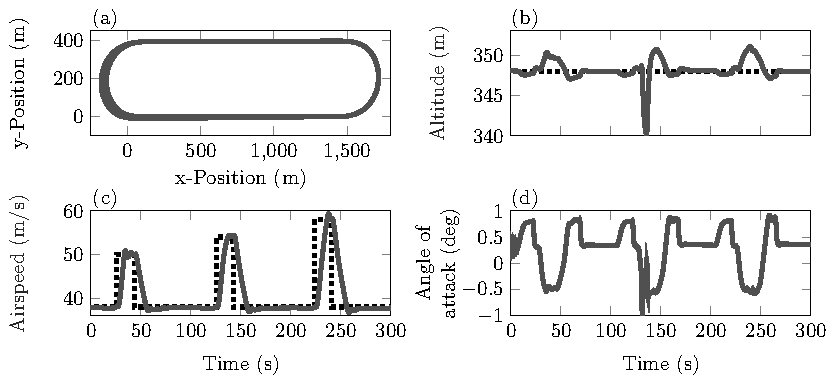
\includegraphics[]{figs/d1_patt_fp.pdf}
	\caption{Simulated aircraft position during three laps on the test track in (a), reference and aircraft altitude in (b), reference and aircraft velocity in (c), and angle of attack in (d).}
	\label{fig:d1_patt_fp}	
\end{figure}


In Figure  \ref{fig:d1_patt_act} the corresponding control surface deflections of the ailerons and the ruddervators are depicted. In diagram (a) the deflections of the two left ($\delta_{a,l2}$, $\delta_{a,l3}$) and the two right ($\delta_{a,r2}$, $\delta_{a,r3}$) aileron pairs used to control the roll motion of the aircraft are shown. Due to selected aileron control allocation described in (\ref{eq:CAail}), the deflections are identical for the two left and two right ailerons, respectively. 
A moderate deflection of  $\approx\pm$\SI{3}{\degree} is necessary to bring the aircraft to the desired bank angle of \SI{45}{\degree} during the turns and back to \SI{0}{\degree}after the turns. In diagram (b) the deflections of the ruddervators are shown, which are the result of the  superposition of the rudder and elevator commands from the baseline controller, following from the control ruddervator allocation in (\ref{eq:CAelev}). Again, the deflections on each side are identical so that only two lines are visible. The deflections of about $\pm$\SI{45}{\degree} around the trim value of $\approx$\SI{8}{\degree} required to ensure the coordinated turn without side slip angle ($\beta \approx 0$) and to track the reference altitude during the turns and on the test leg. Diagram (c) depicts the  deflections of the outer aileron pair ($\delta_{a,l4}$, $\delta_{a,r4}$) between 62\,s and 71\,s simulation time, i.e., when the aircraft is flown within the open-loop flutter regime. The depicted deflections are required to stabilize the aircraft. Only a single line is visible as  in the velocity range up to 58\,m/s the symmetric flutter mode is the predominant, unstable mode.
Diagram (d) depicts the deflections of the outer aileron pair between 164\,s and 173\,s simulation time, i.e., when the aircraft is accelerated to 58\,m/s reference speed. The required deflections for stabilizing the aircraft are comparable to the ones at 54\,m/s airspeed.

\begin{figure}[h]
	\centering
	% This file was created by matlab2tikz.
%
%The latest updates can be retrieved from
%  http://www.mathworks.com/matlabcentral/fileexchange/22022-matlab2tikz-matlab2tikz
%where you can also make suggestions and rate matlab2tikz.
%
\definecolor{mycolor2}{rgb}{0.21990,0.71340,0.72250}%
\definecolor{mycolor4}{rgb}{0.47060,0.00000,0.52160}%
\definecolor{mycolor5}{rgb}{0.52000,0.92100,0.31370}%
\definecolor{mycolor6}{rgb}{0.29630,0.61910,0.85150}%


\definecolor{mycolor1}{rgb}{0.2,0.2,0.2}%
\definecolor{mycolor3}{rgb}{0.7,0.7,0.7}%

\begin{tikzpicture}

\begin{axis}[%
width=2in,
height=0.70in,
at={(0in,0in)},
scale only axis,
title={(a)},
title style = {yshift=-3mm, xshift=-23mm},
xmin=0,
xmax=200,
xtick = {0,50,100,150,200},
ylabel style={align=center},
ylabel={Deflections \\ (deg)},
ymin=-4,
ymax=4,
axis background/.style={fill=white}
]
\addplot [color=mycolor1,solid,line width=2.0pt,forget plot]
  table[row sep=crcr]{%
0	-0.00977646362278599\\
0.12765517889269	-0.00977646362278599\\
0.309687489369266	-0.00977646362278599\\
0.499453484537729	-0.00977646362278599\\
0.532460818657036	-0.000628463417739234\\
0.732863562190875	-0.0158534118368193\\
0.919501787269521	-0.0219421893872442\\
1.11238371376274	-0.0203877055673532\\
1.29990096741374	-0.0196064530840086\\
1.4751627836774	-0.020450206631118\\
1.66922208453841	-0.0215259856395507\\
1.86881391406207	-0.0207350308045709\\
2.06345120039374	-0.0207163514834283\\
2.26222339717595	-0.0214798567666751\\
2.4600542125979	-0.0207542241857099\\
2.65709650277339	-0.0210285679217494\\
2.85632735069452	-0.0214339375118666\\
3.05616293409217	-0.0205911932888335\\
3.25289519736368	-0.0210854728182207\\
3.45	-0.0211731255367406\\
3.65	-0.020444589442594\\
3.85	-0.0210891138448505\\
4.04420102912925	-0.0208365890838122\\
4.24017979905859	-0.020311652289345\\
4.43752665570295	-0.0209865229431527\\
4.63812684810947	-0.0205025654110044\\
4.83722869342592	-0.0202619777722416\\
5.0379110437023	-0.0208622378926179\\
5.23551124874426	-0.0202007815127257\\
5.4348562320492	-0.0202838680237637\\
5.63496657941652	-0.0206957173278853\\
5.83409309304052	-0.0199907186187132\\
6.02982252588517	-0.0203395377571278\\
6.2245916013119	-0.0205267908466095\\
6.42196669724205	-0.0198896069758497\\
6.61926919125825	-0.0203878902849448\\
6.81877063253405	-0.0203448255763792\\
7.01898814214059	-0.0198555999597901\\
7.21848898882136	-0.0204487506353922\\
7.41861741553371	-0.0201415212571676\\
7.61623108278168	-0.0198891558339963\\
7.81668334838103	-0.0204546576418213\\
8.01553612946829	-0.0199650881912213\\
8.21597396554432	-0.0199729845720624\\
8.41670410004718	-0.0203931856452295\\
8.61564676531096	-0.0198136125263984\\
8.8098187216986	-0.0200513152179071\\
9.00904061977074	-0.0202814334820052\\
9.20674654775349	-0.0197250842214576\\
9.4073884499475	-0.0201302468007988\\
9.60631702749725	-0.0201231007970894\\
9.80607243423962	-0.0196813864667002\\
10	-0.0201673391992379\\
10.1971666166312	-0.0199700890086093\\
10.3964581569325	-0.0196836693442543\\
10.5970641125279	-0.0201774217516966\\
10.7976425876413	-0.0197980755929245\\
10.9964672321505	-0.0197446009386699\\
11.1941193544686	-0.0201445637804942\\
11.391666652008	-0.0196787795538776\\
11.5906968332742	-0.0198202838328815\\
11.7907845701609	-0.0200726522558789\\
11.9901530887844	-0.01959877390137\\
12.1911495617973	-0.0199200311457985\\
12.385070665962	-0.0199778583810911\\
12.5861677274275	-0.019576241819993\\
12.7814513299668	-0.0199794656068293\\
12.9812793239324	-0.0198651377643183\\
13.1812597384071	-0.0195992270887025\\
13.3790202986187	-0.0200260065655012\\
13.5780646678143	-0.0197524217614912\\
13.7751912351379	-0.0196540648091393\\
13.9766404849383	-0.0200302463169151\\
14.1749557287324	-0.0196558598738036\\
14.3769470567696	-0.0197471259188039\\
14.5747260527418	-0.0199901477760838\\
14.7750608633794	-0.0195871472606885\\
14.968587338732	-0.0198199215662728\\
15.1254351238164	-0.0199819876352838\\
15.3269888601599	-0.0195915307149588\\
15.5265352125421	-0.0198089768467851\\
15.7255044768762	-0.0199112985394261\\
15.9259000234606	-0.0195633103828496\\
16.1248434175182	-0.019883778047439\\
16.3269706370219	-0.0198149490978724\\
16.5262937961431	-0.0195811648781054\\
16.7253792270448	-0.0199349186223379\\
16.9223525630322	-0.0197284523042533\\
17.1215845125627	-0.0196307414783096\\
17.3227278440507	-0.0199481971706031\\
17.5229007746244	-0.0196475429332073\\
17.7214697203898	-0.0197097588288819\\
17.9163013173114	-0.0199314921815397\\
18.1121096963275	-0.0196099752383143\\
18.3095359616165	-0.0197725697835752\\
18.5095177030575	-0.0198925454523351\\
18.7027959367026	-0.0195940240996227\\
18.9	-0.0198368843879094\\
19.1	-0.0198444211532806\\
19.3	-0.0196053713187099\\
19.5	-0.0199016351565767\\
19.7	-0.0197743279448274\\
19.9	-0.0196507783569247\\
20.1	-0.0199371386997853\\
20.2995912377199	-0.0197115715771376\\
20.4938886306252	-0.0197117960021845\\
20.6884694637955	-0.0199430960253692\\
20.8878618821167	-0.0196824173913654\\
21.0881887874913	-0.0197834711028374\\
21.2887590310582	-0.0199240361273837\\
21.4888744953865	-0.0196626284449068\\
21.6852218915015	-0.0198594897158353\\
21.8843778145349	-0.0198897831299323\\
22.0873773557437	-0.0196781557133199\\
22.2806079753341	-0.0199227044218726\\
22.4815679928946	-0.0198467117561818\\
22.6754122667622	-0.019715076627639\\
22.8775344893606	-0.0199709793354055\\
23.0752181379165	-0.0198129457525793\\
23.2738638150987	-0.0197804076469399\\
23.4689042447237	-0.0199980207416907\\
23.6657426680035	-0.0197962897619593\\
23.8624662644903	-0.0198475593500309\\
24.0626104845773	-0.0200104500027522\\
24.2631832344499	-0.0197921464704604\\
24.462881109226	-0.0199375694515332\\
24.6630658267869	-0.0200047117515396\\
24.8631242332958	-0.0198163151627034\\
25.062587375128	-0.0200237408789316\\
25.2629188125717	-0.0199916102049093\\
25.4632367461522	-0.0198732410229204\\
25.6581323750046	-0.0200954224104547\\
25.85	-0.0199988428661302\\
26.05	-0.0199459698531025\\
26.2473684277957	-0.0201556704893766\\
26.4494146206008	-0.0200068650655208\\
26.6468369187136	-0.0834809912710349\\
26.8459173773743	-0.103068417756235\\
27.0402582770848	0.00183440429480651\\
27.2372870371433	0.0262794913145608\\
27.4355257106277	0.00783709560179269\\
27.6343139526918	0.00203179089838364\\
27.8340909922176	-0.00203254542129821\\
28.0318276963802	-0.00926043057701711\\
28.2311043162899	-0.0144076962125034\\
28.4313510418108	-0.0167731605489141\\
28.6290985530757	-0.0176441866493892\\
28.8294287940124	-0.0184779236834839\\
29.0260558741633	-0.0196138411810827\\
29.2246860748435	-0.0201918999901222\\
29.4256450778754	-0.0204635822343608\\
29.6258611611026	-0.0206720102907012\\
29.8253981415217	-0.020625622279274\\
30.0268695631442	-0.0208758126908813\\
30.221438713447	-0.0211087443520886\\
30.4190984060734	-0.02104521150159\\
30.6168406796266	-0.021221025822554\\
30.8160526932584	-0.0213307711720935\\
31.0165420218093	-0.0213239456977466\\
31.2133871975548	-0.0215984350394577\\
31.4124609048237	-0.0216925739890003\\
31.614167932992	-0.0217655846997029\\
31.8120288171268	-0.0220884551868035\\
32.0100630022558	-0.0222038908817252\\
32.202084313959	-0.0224175174877924\\
32.4037374869747	-0.0228390319628097\\
32.6030681817838	-0.0230544339657082\\
32.8030703668352	-0.0234998943452768\\
33	-0.0240748718780623\\
33.1944831221358	-0.0245344186131018\\
33.3937893178954	-0.0253612824950681\\
33.5945700859505	-0.0263445782627066\\
33.7952818369001	-0.0274446202261871\\
33.9948855435361	-0.0291521073913982\\
34.1911046032595	-0.0312288164244931\\
34.3905242110405	-0.0341259315734796\\
34.5875230678219	-0.0385070232721873\\
34.7880760394402	-0.0451413472458173\\
34.9843497352474	-0.0532113070547145\\
35.1790114495969	0.101783449645845\\
35.3779098278874	0.620742237422052\\
35.5784581471105	1.17001277529855\\
35.7711742205197	1.52159661978203\\
35.9592845571874	1.73330881141372\\
36.1533928559882	1.82145248549436\\
36.3683733183681	1.92515461376958\\
36.5688929518074	1.94302257841197\\
36.7695529623675	1.89975252573005\\
36.968868434667	1.84392799241748\\
37.1688744412883	1.77944890138433\\
37.368653654968	1.7050115385839\\
37.5690573076266	1.62691189846814\\
37.7696165443917	1.5503098866822\\
37.9682179760853	1.47452824023797\\
38.1658315103659	1.40022382645093\\
38.3667712752763	1.32694420844238\\
38.5657510881383	1.25398127030672\\
38.765993622525	1.18339566106497\\
38.9593126538892	1.11725809711002\\
39.1595308547064	1.0508137945726\\
39.3597383564459	0.98676612592417\\
39.5590635585905	0.924865221357918\\
39.7564771921748	0.865499330087696\\
39.9571335380653	0.808638992571388\\
40.1562381313717	0.753927691707523\\
40.357094277611	0.700933422661627\\
40.5566622364659	0.6513710047832\\
40.7561386235215	0.603828814397468\\
40.9559470223116	0.558760930588295\\
41.1562979450914	0.516206521174573\\
41.3570491782741	0.475775604503305\\
41.5571514473329	0.437851321500599\\
41.7562696151345	0.402451100331607\\
41.9571617421779	0.368929950728151\\
42.1567368983106	0.337763922804605\\
42.3516755071619	0.309289005011463\\
42.55	0.282023872205774\\
42.7434765206129	0.257415525586157\\
42.9411685707452	0.234039005323479\\
43.1337705434646	0.212793034100595\\
43.330987314291	0.192679706642784\\
43.5332041708185	0.173669552229449\\
43.7278677243602	0.156542895445039\\
43.925017064506	0.140329129173457\\
44.1212995675028	0.12549802845695\\
44.3187254086058	0.111695140596591\\
44.5188778187032	0.0989597354104269\\
44.719995699826	0.0870911213289379\\
44.9185460823373	0.0762798063722726\\
45.1205219297252	0.0661610879151856\\
45.3199730710157	0.0570372163707846\\
45.5184747106513	0.0487107666176777\\
45.7192482926822	0.0410026218984339\\
45.9190248801686	0.0340579612187074\\
46.1156673854361	0.0277844727568314\\
46.3100357058516	0.0220427905178537\\
46.5090986580926	0.0168572596506451\\
46.703285998475	0.0123308752390301\\
46.9	0.00814847578857165\\
47.1	0.00427933545117949\\
47.3	0.000867413074860027\\
47.5	-0.00217635768119519\\
47.7	-0.00504058225420992\\
47.9	-0.0076815392587693\\
48.0992342057289	-0.00996298536352919\\
48.2942242492551	-0.0122368226242319\\
48.4934096077188	-0.014152635084474\\
48.6923151504599	-0.0156856461916712\\
48.8849438384061	-0.017176408524282\\
49.0841507592169	-0.0187317343209317\\
49.2819427170925	-0.0198690205295137\\
49.4807701783885	-0.0209533076699633\\
49.6800836829276	-0.0220902438610635\\
49.8790185010079	-0.0230911904276656\\
50.0778471512413	-0.0238967398739948\\
50.2767547042535	-0.0248379504409076\\
50.4696939175188	-0.0256238110406738\\
50.6691529368966	-0.0264902982977755\\
50.8661900621746	-0.0269596173612686\\
51.0653818741547	-0.0275116699334596\\
51.2656946698371	-0.0284159033786808\\
51.4668387765167	-0.193987898031956\\
51.6654392391431	-0.755784729860882\\
51.8626812279047	-1.43227534377371\\
52.0626408496778	-2.0655554942877\\
52.2624716605855	-2.61137165760057\\
52.4630581927788	-3.001616396262\\
52.6631267836445	-3.17697258172505\\
52.86309606766	-3.15141841569495\\
53.0633965995946	-2.98395204450124\\
53.2731655140825	-2.72870287946004\\
53.4725570439538	-2.46235409461306\\
53.6730229077079	-2.20392974856099\\
53.8719761733441	-1.97538846101819\\
54.0692946303923	-1.78230770124178\\
54.268292233522	-1.61785726169855\\
54.4658159559313	-1.47777322416783\\
54.6631671684759	-1.35365885002125\\
54.8623981536957	-1.23923943198104\\
55.0628018062972	-1.13193921558279\\
55.2621321917579	-1.03037345300328\\
55.4595622401205	-0.933522104270526\\
55.6602456985741	-0.838595324628321\\
55.8594620173921	-0.472892557029362\\
56.0600594637766	1.15322848990281\\
56.2445063470183	0.332182820392911\\
56.4134970152377	-0.888283368923778\\
56.6118982528325	-1.21594071178171\\
56.7817467545294	-1.05354190017289\\
56.9530393022815	-0.906617354624875\\
57.1596328397402	-0.716318387569856\\
57.3437171688974	-0.506731173309512\\
57.5317086374579	-0.335144868032279\\
57.7532871982145	-0.218471362693212\\
57.9530815692416	-0.159068463726088\\
58.1536155091825	-0.118075248668929\\
58.3536902910293	-0.0852065061189739\\
58.5532453395971	-0.0620745477011109\\
58.7529980719605	-0.0497455300656481\\
58.9532786650139	-0.043417035843939\\
59.153837399268	-0.0374203541028505\\
59.353147500179	-0.0310720914582876\\
59.5535639908845	-0.025941239404874\\
59.7535891595181	-0.022207111567715\\
59.953468029942	-0.0195041658979219\\
60.0812440750265	-0.0179563271772847\\
60.1914563239107	-0.0169400996869285\\
60.2995354599956	-0.016902136831039\\
60.3953639007809	-0.0153215733828861\\
60.4941021856542	-0.0137343355440965\\
60.5945243501064	-0.0130737758412628\\
60.6852627904763	-0.0126752145396705\\
60.7851065860043	-0.0131421532640953\\
60.8813485595584	-0.0141167836706363\\
60.9847712262535	-0.0145736035154079\\
61.0870402702917	-0.0149598626087109\\
61.1777457376203	-0.0151391460956196\\
61.2668562952212	-0.0148740823718211\\
61.3596285266116	-0.0155740033757568\\
61.4573804469686	-0.0163554328016484\\
61.5557297555814	-0.0167035010959497\\
61.6517799692959	-0.0165143989408558\\
61.7512466968806	-0.0160279928585134\\
61.8642985646118	-0.016089057608468\\
61.9906527667507	-0.0165583113245481\\
62.1115324121344	-0.0169183937914253\\
62.2164153195816	-0.0167370505661474\\
62.3128770374205	-0.0172984907577166\\
62.403791155791	-0.017987618161014\\
62.4957806627064	-0.0178158244729929\\
62.5918547232226	-0.0182536042721013\\
62.678920100231	-0.0179078625197631\\
62.766900658444	-0.0181048844113703\\
62.8575220560467	-0.0190867885028867\\
62.9406015425199	-0.0183153822547176\\
63.0185634550891	-0.0198587942397244\\
63.0951628784741	-0.0201858552956833\\
63.1708977083699	-0.0195581034110722\\
63.2469072999021	-0.0196212788325231\\
63.3229839530985	-0.0196921979441596\\
63.3980526006882	-0.0178756177577384\\
63.4726561277579	-0.0176482467561386\\
63.55	-0.0183175133612213\\
63.6269728390634	-0.0194822315638145\\
63.7035512809945	-0.0211137795660492\\
63.7815075142097	-0.020242094662691\\
63.8611352442331	-0.0181912810651183\\
63.9429555074285	-0.0170876609716217\\
64.0279110736533	-0.0174611496406871\\
64.1154714379754	-0.0193387147672388\\
64.2024823151694	-0.0209309524888068\\
64.2847233499973	-0.0207392410082063\\
64.364728389895	-0.0194459430563191\\
64.4426598723772	-0.0198002739281006\\
64.5169626280015	-0.0203168460528976\\
64.5922017210998	-0.0227408862921721\\
64.6654815602183	-0.0231337361272929\\
64.7382683144206	-0.0238491195705312\\
64.8096271557676	-0.0225484565410035\\
64.8812569814245	-0.0230291926041291\\
64.9532547085529	-0.0229071780649282\\
65.0252717286516	-0.0245114223935048\\
65.0974590278137	-0.0251992513484643\\
65.1675607075392	-0.0255665223777706\\
65.2354790552826	-0.0249587647472611\\
65.3031386066194	-0.0244708765472102\\
65.3719345870124	-0.0240325027494606\\
65.440225652876	-0.0245464915244721\\
65.5099921132134	-0.0250653400750611\\
65.5820455247	-0.0261548880070044\\
65.6556578065739	-0.0263633059762495\\
65.7288172591662	-0.0265714488385718\\
65.8021145481074	-0.0265636595167774\\
65.8785981437047	-0.0256658205245774\\
65.9573308730737	-0.0260987122869792\\
66.04064622609	-0.0250962477824436\\
66.1270560778165	-0.0250408359096323\\
66.2084117911707	-0.0241104461368612\\
66.2840203021821	-0.0239146580932665\\
66.3578993562952	-0.0228549788448255\\
66.4277763228401	-0.0234958908236414\\
66.4982362661441	-0.0223933534659594\\
66.5677792700214	-0.0234080981214534\\
66.6360560358152	-0.0222742675837817\\
66.7056536969589	-0.0229854394903212\\
66.7739801764402	-0.0221685430621921\\
66.8416355874517	-0.0224356327852049\\
66.9095732855869	-0.0223183553214425\\
66.980567343459	-0.0222597962108488\\
67.0550160653393	-0.022187643936738\\
67.1270050095338	-0.0221495890898163\\
67.1976580306412	-0.0224066222018256\\
67.265798524604	-0.0216858354383493\\
67.3353780842613	-0.0227931066382733\\
67.4042262821641	-0.0215158556171541\\
67.4749062138197	-0.0229255774865698\\
67.5443124106559	-0.0217590000352855\\
67.6167382623251	-0.0225628295025188\\
67.6920395019771	-0.0222446264565111\\
67.7675017803082	-0.0221762784840098\\
67.8417800590381	-0.0223940276617589\\
67.9208469907054	-0.0224603352338592\\
68.0053820885573	-0.0222131113268677\\
68.0895720791161	-0.0226302091367641\\
68.1747840143076	-0.022556851553924\\
68.2561268120414	-0.0225632643429287\\
68.3329523738923	-0.0227499602957058\\
68.4080198851637	-0.0228234630938492\\
68.4822014671048	-0.0227454185867246\\
68.5552558930557	-0.0231671850668048\\
68.6302916004756	-0.0226629909483302\\
68.7032310448858	-0.0235417834173108\\
68.776465120216	-0.0226639940592553\\
68.8485247331509	-0.0238183630489693\\
68.9208562537114	-0.0227786936080986\\
68.9947705990121	-0.0239291723451257\\
69.0684342337102	-0.0231831622932572\\
69.1433366883293	-0.0236774367340382\\
69.2150904618601	-0.0238019967090155\\
69.2863675625967	-0.0235770223776156\\
69.3562009919975	-0.0241560163459116\\
69.4282790746872	-0.0241393050341495\\
69.5	-0.0242366610432544\\
69.5740710974609	-0.0249438692556607\\
69.6489374165234	-0.024540151849698\\
69.7239410880034	-0.025359785768621\\
69.801226101595	-0.0257545755944654\\
69.8798556078153	-0.0258072303955038\\
69.9612013032615	-0.0263710084704317\\
70.0405587352092	-0.0263522060491704\\
70.130614413897	-0.0261010379683634\\
70.2289745454876	-0.0261900441348562\\
70.3333968156943	-0.0260849182834292\\
70.45	-0.0258324317339372\\
70.5785775011778	-0.0253715824427049\\
70.7210862289691	-0.0247501679233874\\
70.8750172665248	-0.0243263831275714\\
71.0436174010324	-0.0241548304131315\\
71.2098281421034	-0.0241579945257539\\
71.3733249206709	-0.0247580993313466\\
71.5288835635502	-0.0251397998317048\\
71.6903650869855	-0.0251898106334476\\
71.85	-0.0255383265606976\\
72.009132146522	-0.0258054791490091\\
72.1658783010117	-0.025922892167212\\
72.3247415446502	-0.0262401122164553\\
72.486775651293	-0.0264742797006302\\
72.6452163656339	-0.0266292107383039\\
72.8053404602228	-0.0268845201182643\\
72.9622172989879	-0.0270087447159835\\
73.1154767039992	-0.0270728331141213\\
73.27315949072	-0.0271792266863701\\
73.4288718055083	-0.0271783305947177\\
73.5865832724247	-0.0271281193950709\\
73.7421301140358	-0.0270929391561318\\
73.8950810248513	-0.0269913918070146\\
74.0526919560948	-0.0269006132927746\\
74.2073527576493	-0.0267349758558285\\
74.3615843485503	-0.0263751793421478\\
74.5175848959321	-0.0260358534101908\\
74.67377127598	-0.0258026474292568\\
74.828940241504	-0.025541808511216\\
74.9859911118744	-0.0253161085143084\\
75.1426309188082	-0.0251711696272232\\
75.3	-0.0250123453510207\\
75.459783604731	-0.0248735557608979\\
75.6197971294396	-0.0247868159240196\\
75.7791647451796	-0.0246816983845826\\
75.9415746919365	-0.0245872134603716\\
76.1	-0.0245107827154091\\
76.2629858587324	-0.0244240334672732\\
76.4267094073267	-0.024345473900549\\
76.5910061284987	-0.0242778530001791\\
76.7581103803916	-0.0241929306166872\\
76.9232283953467	-0.0240993643190353\\
77.0883069904238	-0.0240183431185454\\
77.2552346307122	-0.0239506428598977\\
77.4244435946884	-0.0238577342515236\\
77.5988116658253	-0.023753678808532\\
77.7660628016482	-0.0236641222170693\\
77.936111531218	-0.0235768644293038\\
78.1081758558621	-0.0234778565769109\\
78.2792316730057	-0.0233776963713157\\
78.4490514136398	-0.0232834681162801\\
78.6224313740068	-0.0231841491806104\\
78.7967969141945	-0.0230821484281789\\
78.9850467818154	-0.022973683354435\\
79.1840369622761	-0.022860051507544\\
79.3825631807418	-0.0227455197530017\\
79.5820031309474	-0.0226304038770001\\
79.7836235770329	-0.0225157687958041\\
79.9827585815433	-0.0224030341839285\\
80.181263195259	-0.0222914396267181\\
80.3818269898738	0.033165956394421\\
80.5818298150351	0.462019747342504\\
80.7814349854115	1.07367320665843\\
80.9616560725625	1.4877669698156\\
81.1386782293474	1.75828212792106\\
81.3173784207353	1.93015378420493\\
81.5034473561729	2.01559993489083\\
81.7038140364635	2.02882284945017\\
81.9038285355578	1.99060270066903\\
82.1037946594693	1.92855582873654\\
82.3100499503017	1.85097488656817\\
82.5230491858938	1.75783980311626\\
82.7227528876449	1.66143934669311\\
82.9218179304147	1.56966572658621\\
83.1225776122753	1.47703535916722\\
83.3236961476038	1.38495453353441\\
83.5191959910117	1.29637100962612\\
83.7181238003833	1.2100080213618\\
83.9157581066543	1.12541858410423\\
84.1136500814762	1.0439399734715\\
84.3124755348568	0.965278192261392\\
84.5070720712354	0.890572349051784\\
84.7064243880485	0.817468778344835\\
84.906517144461	0.747031230650581\\
85.1069707737403	0.679558844869683\\
85.3062715462545	0.615494437433414\\
85.5061458657463	0.554638312874547\\
85.7066175295547	0.496914033011963\\
85.9070200276406	0.442286159667463\\
86.1072764781867	0.390982238754291\\
86.3065904036746	0.343306608399248\\
86.5063320314316	0.299846920648818\\
86.706571323459	0.261751544395106\\
86.9061466697194	0.22919453127224\\
87.1061450735719	0.20224578116274\\
87.3062247680557	0.180460808121884\\
87.5062794391903	0.163505835056894\\
87.7	0.15113307544013\\
87.8991745181882	0.14256295687911\\
88.0969433081854	0.13750479235829\\
88.2974341161454	0.135703595864983\\
88.4968610355758	0.136522840681611\\
88.7	0.139581081911696\\
88.8960818379444	0.143694515335096\\
89.0937921259516	0.14862317950688\\
89.2911636255814	0.153764645575726\\
89.4914410065878	0.15850552451157\\
89.6906125601225	0.161998183517202\\
89.8911301912251	0.163535603344465\\
90.0901528811153	0.162720935512761\\
90.2874279126955	0.159202210409538\\
90.4879672621049	0.152891568266909\\
90.6884339862072	0.143750386595548\\
90.8875830045818	0.131870533451753\\
91.0882469755054	0.117431668488015\\
91.2905463377903	0.101028565158446\\
91.4890183911262	0.0836554783004558\\
91.6854714822511	0.065864238936874\\
91.8845548883453	0.0479875910625929\\
92.0792564177483	0.0313239390289463\\
92.2792586969852	0.0158165678124262\\
92.4781844471918	0.00236424864931162\\
92.6792386316064	-0.00925266866297791\\
92.8777665976364	-0.018462846877397\\
93.0736214626573	-0.0255562631585274\\
93.2695247083015	-0.0304541416170007\\
93.4684541282135	-0.0335568211236986\\
93.6692170887673	-0.0349619863570198\\
93.8698375245211	-0.034955526748701\\
94.0686774915692	-0.0339622853810559\\
94.2663916957428	-0.0322489038722194\\
94.4674656439482	-0.0298734130888136\\
94.6663876594465	-0.0269575527469913\\
94.8666945816078	-0.0239961473666792\\
95.0653729494554	-0.0211039754900131\\
95.2661664367548	-0.0184246675687425\\
95.4670050091161	-0.0160623144175259\\
95.6651440686382	-0.0142443388574626\\
95.8583226253887	-0.0131355765416867\\
96.0560833836232	-0.0127844847772576\\
96.25	-0.0128469312863147\\
96.4495163091454	-0.0132885184739519\\
96.6474513230581	-0.0620635667871122\\
96.8474266056036	-0.479427235053663\\
97.0484574207874	-1.15904958091564\\
97.2473699406742	-1.81878355287866\\
97.4468206599105	-2.40658313631825\\
97.6477065718706	-2.87206721677241\\
97.8483869384157	-3.13687333585557\\
98.0482680434615	-3.18609471713529\\
98.248694184592	-3.06692120021558\\
98.4495189551183	-2.84638656699697\\
98.6466012243581	-2.58840361031132\\
98.8426727477622	-2.32819669921693\\
99.0413452859993	-2.08445856807542\\
99.2418536553608	-1.87113618940851\\
99.4409539193611	-1.69229156060798\\
99.6375199024252	-1.54200566553451\\
99.8373937110535	-1.40845496489999\\
100.03519747834	-1.28942968415557\\
100.233853694275	-1.1789299538133\\
100.431319095129	-1.07540921627589\\
100.628804392263	-0.976212104147747\\
100.828268465054	-0.879692693926674\\
101.029920735322	-0.785797570325829\\
101.228058926064	0.626543485917348\\
101.423688086578	0.908443581615057\\
101.596297526156	-0.439676417775473\\
101.787416017288	-1.19130844485324\\
101.969079409903	-1.11130899177413\\
102.138094477037	-1.01500057629336\\
102.32936256833	-0.861511797013947\\
102.532744204027	-0.554272442417707\\
102.721496236055	-0.340027863756321\\
102.925498061402	-0.217903230033835\\
103.15	-0.144026976801275\\
103.35	-0.10460308196357\\
103.55	-0.0774491292814679\\
103.75	-0.0561910761004794\\
103.948273552385	-0.0427540523973782\\
104.146770289033	-0.036305012915203\\
104.346770664716	-0.0325051834639374\\
104.5420408188	-0.0286265953423809\\
104.742200600864	-0.024692710175834\\
104.941157434339	-0.0217777791714522\\
105.14239512668	-0.0199327921132696\\
105.341383922914	-0.0185439064186253\\
105.541370186419	-0.0180051107207973\\
105.741551125403	-0.015465537822738\\
105.941132598884	-0.0136530336869396\\
106.141474684466	-0.0135575539159196\\
106.340478847287	-0.0135838681294768\\
106.541206773191	-0.0135339664140851\\
106.741427167307	-0.013591286845377\\
106.941048734975	-0.0137506933101883\\
107.140844849006	-0.0139346570640702\\
107.341348022979	-0.014110515085143\\
107.540740513663	-0.0143081333062257\\
107.744137034137	-0.014494773887318\\
107.943126888314	-0.0146750897156415\\
108.143668941012	-0.0148735924536952\\
108.344287707504	-0.0150503184934443\\
108.54488316915	-0.0152214961442153\\
108.744150341822	-0.0154014405480441\\
108.941163187435	-0.0155554548076558\\
109.140467951693	-0.0157131572254722\\
109.340728735127	-0.0158756624562343\\
109.533795184519	-0.016010920369595\\
109.734109701293	-0.0161551425339696\\
109.928656351925	-0.0162958366223401\\
110.128138852588	-0.0164164869320491\\
110.325273438513	-0.0165491155013389\\
110.527165524986	-0.0166735097230324\\
110.7247800428	-0.0167809652918266\\
110.925507742489	-0.016902679497986\\
111.124567260059	-0.0170075880487105\\
111.321856959917	-0.0171027332240981\\
111.519377716176	-0.0172096973811163\\
111.718097837789	-0.0172979839965357\\
111.916106884947	-0.0173847824635796\\
112.116745661189	-0.0174803475746936\\
112.315687413951	-0.017555259231271\\
112.51590360122	-0.0176361562603989\\
112.716897745809	-0.0177195995127376\\
112.915306727191	-0.0177827980652262\\
113.113304881853	-0.0178577998167376\\
113.312213015925	-0.0179280730644909\\
113.509213350975	-0.017983986116498\\
113.703198557981	-0.018052064930923\\
113.903581351429	-0.0181125380211598\\
114.103090788398	-0.0181643494994524\\
114.303198212923	-0.0182295392697289\\
114.503100218178	-0.0182807767964066\\
114.7	-0.0183285281042949\\
114.9	-0.0183877293453464\\
115.1	-0.0184308771317828\\
115.3	-0.0184777981057092\\
115.5	-0.0185309437838163\\
115.69965223238	-0.0185673782650185\\
115.895912436634	-0.0186121392896283\\
116.088277465104	-0.0186571865113151\\
116.288217542197	-0.018688665163982\\
116.487888407784	-0.0187326144795591\\
116.687273773475	-0.018772095706588\\
116.887614788259	-0.0188010495040065\\
117.088136691407	-0.0188432654985184\\
117.289095052159	-0.0188753648462244\\
117.487358779202	-0.0189031109505936\\
117.688013344832	-0.0189424994130025\\
117.887100611162	-0.0189682906108338\\
118.084413624542	-0.0189958699534298\\
118.285071530416	-0.019031508417283\\
118.484828152603	-0.0190530016417681\\
118.684314180937	-0.0190816080365036\\
118.884918175605	-0.0191128828430376\\
119.084324427388	-0.0191315033763289\\
119.284654593237	-0.0191610372860869\\
119.485436126514	-0.0191876194141208\\
119.684416560104	-0.0192052983241715\\
119.884809121604	-0.0192352164151173\\
120.083925407911	-0.019257140893965\\
120.285922756878	-0.019275812131073\\
120.480154689037	-0.0193044638490983\\
120.678494642603	-0.019322846527298\\
120.872050426593	-0.0193418645555217\\
121.072181195516	-0.0193699939537156\\
121.27212792638	-0.0193863323747316\\
121.47246301434	-0.0194082305945041\\
121.668252285923	-0.0194339316628277\\
121.865570868701	-0.0194487975699222\\
122.065592801444	-0.0194726712546038\\
122.265711046514	-0.0194967167806697\\
122.466939055309	-0.0195121269221276\\
122.666513897231	-0.0195382365880206\\
122.865384661861	-0.0195597183252383\\
123.063125016302	-0.0195764424782562\\
123.262522810586	-0.0196041155110807\\
123.463409003934	-0.0196241822833413\\
123.663304656488	-0.0196441467943525\\
123.864080375311	-0.0196730302822853\\
124.06257578871	-0.019692206228704\\
124.26354436952	-0.0197164123461498\\
124.462507657745	-0.0197456953698763\\
124.663065286224	-0.0197661673074092\\
124.859371893145	-0.0197943183549604\\
125.059353263579	-0.0198246582825383\\
125.259672740338	-0.0198481065002827\\
125.459504174971	-0.0198818944692463\\
125.659956593946	-0.0199136674661512\\
125.860588472327	-0.0199423297927259\\
126.055809676168	-0.019980848465331\\
126.253588488584	-0.0200153933162468\\
126.45	-0.0200502254240928\\
126.65	-0.0200962011075821\\
126.85	-0.0201362688390118\\
127.05	-0.0201817595393447\\
127.25	-0.0202355642644223\\
127.447297613939	-0.0202837200731288\\
127.646450357186	-0.0203420136420802\\
127.843823314417	-0.020405978066738\\
128.044617905982	-0.0204686377648985\\
128.243527170366	-0.0205436615388589\\
128.438118639029	-0.0206220425421341\\
128.637294892951	-0.0207045795192761\\
128.83773044199	-0.0208036883409235\\
129.031763529299	-0.0209046081701212\\
129.230782714807	-0.0210176719130191\\
129.428649744103	-0.0211494671232517\\
129.628755256928	-0.021291543689809\\
129.827998153336	-0.0214505933050844\\
130.031450906577	-0.0216409782149162\\
130.228634770943	-0.0218408306804315\\
130.429510164419	-0.0220799688695875\\
130.625185288629	-0.0223479982215667\\
130.827501572249	-0.0226625761818555\\
131.024893501555	-0.0230246664661398\\
131.21967475898	-0.0234443871771242\\
131.418624016761	-0.0239472568103077\\
131.618756181554	-0.0245595216355392\\
131.812345526038	-0.0252706871904406\\
132.012746239496	-0.0261781040723617\\
132.209839315473	-0.0272939843169437\\
132.410552037885	-0.0287339002195812\\
132.609785243324	-0.030591091509467\\
132.803432236737	-0.0329946755358809\\
133.00326960297	-0.0364001349482504\\
133.203557371042	-0.0556202065376312\\
133.399566113433	-0.255811465833241\\
133.59796507424	-0.113544506475816\\
133.794839636155	0.103014059104202\\
133.995584636525	0.529362369222431\\
134.193985581525	1.07922254637452\\
134.386635859415	1.47609578952754\\
134.57456113833	1.71632726944375\\
134.769234168636	1.90237147489319\\
134.977429004248	1.93865733420056\\
135.18521243761	1.91161918883799\\
135.384436044027	1.88375020600265\\
135.585179660599	1.84018201954498\\
135.783804565682	1.77955631687112\\
135.984719520619	1.7119461564049\\
136.18494694015	1.64048190276351\\
136.384148345495	1.56642934878126\\
136.585252601087	1.4913408886393\\
136.78494522933	1.41705677187893\\
136.985573609477	1.34332359810209\\
137.184466364879	1.27170826301707\\
137.381206904302	1.2020109299859\\
137.581501498304	1.13352042380303\\
137.781994207196	1.06676920062156\\
137.982218504613	1.00198829688506\\
138.181675793173	0.939869762164319\\
138.381728466309	0.879865502416092\\
138.581340982418	0.821946454290541\\
138.775516597583	0.768004172138666\\
138.976601610657	0.715133302356885\\
139.174995756634	0.665100621506922\\
139.375767641204	0.616884734424579\\
139.574789535519	0.571405819954003\\
139.771881711096	0.528802673809739\\
139.972464446926	0.48798963220081\\
140.171690997926	0.449591381559178\\
140.372421189212	0.413314359087143\\
140.572708643676	0.379279283745165\\
140.772809086169	0.347442192959654\\
140.969576867874	0.318008659584562\\
141.16961946136	0.290328378973172\\
141.369238973075	0.264573257675467\\
141.570572397958	0.240303054652885\\
141.765284736989	0.21840293818977\\
141.96281669266	0.19769080694513\\
142.16330758811	0.1784378929274\\
142.362384856311	0.1606834735809\\
142.562591775944	0.144078118994698\\
142.756089753917	0.129077991267585\\
142.957068874939	0.114787838557348\\
143.156562115694	0.101941190054446\\
143.357870596727	0.0898101774558533\\
143.556025343949	0.0787749433710453\\
143.75	0.0687644603033935\\
143.945261135828	0.0595368978628082\\
144.144134649779	0.0510178002887004\\
144.344530760472	0.0433572757040122\\
144.543358000733	0.0363481185369546\\
144.738009565519	0.0298456802297877\\
144.93717968939	0.0238833958199236\\
145.134323555467	0.0185736623392314\\
145.335031027687	0.0137179299547561\\
145.534296594552	0.00942810028185271\\
145.731512296419	0.00543771370945359\\
145.924727357706	0.00178386506001593\\
146.124539718643	-0.0015397857749212\\
146.319181741192	-0.00438432065348303\\
146.520556487399	-0.00704268638191214\\
146.718792107821	-0.00920046340437412\\
146.919557532134	-0.0113991735201998\\
147.11841319157	-0.0133699479906945\\
147.319496079355	-0.0151967490298834\\
147.515556232241	-0.0167939762878724\\
147.715892737363	-0.0183856812577478\\
147.91315951059	-0.0197264698452122\\
148.112700069446	-0.0208990149136298\\
148.312947667746	-0.0219179222673996\\
148.513613605021	-0.0229466092842602\\
148.708774878113	-0.0238904465493532\\
148.907045905894	-0.0249351277964757\\
149.103058641401	-0.0256892113066595\\
149.303064857593	-0.0262994238408266\\
149.503066962002	-0.0268947757112045\\
149.703489536944	-0.027481876360467\\
149.90358298952	-0.0280683622927308\\
150.1	-0.121846587597744\\
150.299236826232	-0.613286070476941\\
150.498418682831	-1.29434471937298\\
150.697299515218	-1.93839623440057\\
150.896746607769	-2.50592600559369\\
151.097772785347	-2.93720058579398\\
151.298233985918	-3.15937849292216\\
151.498090976299	-3.17216683369018\\
151.698766370527	-3.02861854327822\\
151.906306525124	-2.78748967488045\\
152.103061397094	-2.52640555201459\\
152.298269357104	-2.27025337792505\\
152.498356650246	-2.03175453228514\\
152.694361985483	-1.83087799945063\\
152.893913837626	-1.65816807377977\\
153.093647397325	-1.51084325670568\\
153.291110630535	-1.38284423340276\\
153.490201526295	-1.26574158382455\\
153.686205476592	-1.15885522020899\\
153.878089185821	-1.05958139648059\\
154.075098380286	-0.96158945330171\\
154.272754424138	-0.866872776675508\\
154.471942127827	-0.764170845845708\\
154.672442058916	0.836563307473345\\
154.867086033117	0.749462937678495\\
155.038263654838	-0.604812180440112\\
155.231181625411	-1.21975349271\\
155.408128134722	-1.10267073192635\\
155.577627355925	-0.944305244344635\\
155.779863569717	-0.771715541093861\\
155.967338811344	-0.563067395298373\\
156.153380761104	-0.375821023065695\\
156.367022974134	-0.242686796349586\\
156.568644998708	-0.17352781006636\\
156.768902288388	-0.129078553500631\\
156.968904085224	-0.0942104373958251\\
157.16838788665	-0.0678901915919109\\
157.366296947461	-0.0524763572267989\\
157.566771612646	-0.0446022753555932\\
157.765836456099	-0.0389769586550065\\
157.966374358238	-0.0331766967357067\\
158.166738949621	-0.0280924943128386\\
158.36588051875	-0.024727489462178\\
158.566233705101	-0.0224743692826503\\
158.766278014737	-0.0203618231281683\\
158.966585013338	-0.0197563511891503\\
159.168706807122	-0.0159650210793232\\
159.370312361293	-0.0140115508718456\\
159.57321217911	-0.0142985257148486\\
159.772107530643	-0.0143064690832342\\
159.973332314646	-0.0144183836636938\\
160.168641392103	-0.0146794388117472\\
160.369554530502	-0.0149777783894801\\
160.570726890158	-0.015438122415409\\
160.770739757894	-0.0157847998039435\\
160.967609607651	-0.0162155639985268\\
161.159653166568	-0.0166675359906122\\
161.3466158277	-0.0170534450503143\\
161.528810598919	-0.0174968924333747\\
161.702467361323	-0.0178808345887133\\
161.8742665226	-0.0181997232770237\\
162.041931881765	-0.0185830712203579\\
162.209888393032	-0.0189472601558275\\
162.380598510974	-0.0192810326057524\\
162.549632082161	-0.0196512935417424\\
162.710532396263	-0.019976138894145\\
162.87607517788	-0.0202842113133549\\
163.040343567075	-0.0206251521194165\\
163.202316803873	-0.0209344842455884\\
163.365062073596	-0.0212388389878205\\
163.527907185435	-0.0215567062146282\\
163.690630843835	-0.02184554770671\\
163.85	-0.0221375441431702\\
164.009600375304	-0.0224351808483963\\
164.163790467245	-0.0216425492042535\\
164.317180187828	-0.0117409743892662\\
164.468707718421	0.00666886231376721\\
164.625697686924	0.0191855908663529\\
164.779586794475	0.0138311924860972\\
164.932109558052	-0.00204652850676468\\
165.05	-0.0130784448435594\\
165.140601380677	-0.0184211552290758\\
165.22056663577	-0.0207409200424588\\
165.297184087573	-0.0226147793937125\\
165.370967235387	-0.0235137219854285\\
165.441695002363	-0.0268063950160949\\
165.511669320907	-0.0290154822451845\\
165.580448092945	-0.0352178778383667\\
165.647867888305	-0.0389308750509793\\
165.715618700963	-0.0465529449477488\\
165.781470009564	-0.0509629327248775\\
165.848703444845	-0.0573445247104053\\
165.917165793816	-0.0622678115941586\\
165.988044108988	-0.0665125547057906\\
166.066164247259	-0.0707383542875803\\
166.13774624797	-0.0730512922810253\\
166.203716553775	-0.0782353832651159\\
166.268715108535	-0.0814760512443014\\
166.33659067405	-0.0891163427628873\\
166.403365213478	-0.0914092085620482\\
166.471920138852	-0.0946181580932001\\
166.542018972566	-0.0916522373383455\\
166.614027370081	-0.0861227578122978\\
166.687394049648	-0.0778833361626839\\
166.760613323481	-0.0677942072428401\\
166.83494902882	-0.0604789351403246\\
166.910401586939	-0.0526048197708498\\
166.991414075545	-0.0490836096484907\\
167.082128972008	-0.0453594186380323\\
167.169380242029	-0.0421069851290802\\
167.246841168527	-0.0347544496820267\\
167.317385549896	-0.0252652831902585\\
167.387431690092	-0.0107854475807407\\
167.456450398956	0.00240038183011705\\
167.525214073791	0.018083814965262\\
167.594088958902	0.0273648486465637\\
167.660335624652	0.0366114994229421\\
167.726976118829	0.0376497412701315\\
167.79492959981	0.0391565129563394\\
167.862699880338	0.034353653360241\\
167.932267099677	0.0312412087234611\\
168.003605438666	0.0251937214024646\\
168.078654572263	0.0217971302979497\\
168.148797560902	0.0186292776670716\\
168.218076693252	0.0160345885179626\\
168.285930650607	0.0131486179567076\\
168.352219672503	0.00587614771733888\\
168.41907152335	-0.000867477899961363\\
168.487200182008	-0.0135094155240719\\
168.55855309064	-0.0241759155809018\\
168.630302779206	-0.0364191735639284\\
168.706790262406	-0.0447247186808796\\
168.778917378814	-0.0497881309221189\\
168.852492444038	-0.0514445106843706\\
168.929681313042	-0.0512514081247972\\
169.014259252932	-0.0497155512706731\\
169.102489303179	-0.0497872263878258\\
169.186388695145	-0.0502696703595694\\
169.263094863456	-0.0514855077967543\\
169.334596068797	-0.0504333656453707\\
169.404109209608	-0.0473741633074879\\
169.472880577536	-0.0431826210916685\\
169.541524579866	-0.0359339775132048\\
169.608068701554	-0.0322097794358504\\
169.67434390074	-0.0254644213027234\\
169.741648074055	-0.0260477953103381\\
169.807081610782	-0.0233072040886955\\
169.873620850662	-0.0276246466390046\\
169.943867107289	-0.0287095049437398\\
170.0170902869	-0.0335625222420255\\
170.090973121323	-0.0349730100899031\\
170.159427192937	-0.036347695628381\\
170.227880698775	-0.0364684450914025\\
170.293137341612	-0.0339674368735437\\
170.359383291687	-0.0337547639440226\\
170.426333355307	-0.0294727351685248\\
170.494588060274	-0.0292220362811572\\
170.566763662762	-0.0260395655249808\\
170.641820157094	-0.0260796715815173\\
170.715486350526	-0.0254419494393335\\
170.788013474632	-0.0262999661814301\\
170.861068156843	-0.027022895736423\\
170.938125713834	-0.0282154477353488\\
171.024231307643	-0.0285826459882096\\
171.114456117799	-0.0294299330672015\\
171.195567803406	-0.0284929734286229\\
171.270677570737	-0.0283524542568145\\
171.341260945807	-0.0272881807557814\\
171.411299483125	-0.0265432558691653\\
171.4787234138	-0.0264707793146562\\
171.547487093633	-0.0249852464541563\\
171.615320478689	-0.0264958303891217\\
171.682595772255	-0.0243225544327045\\
171.748402075747	-0.0271328811940464\\
171.813362047706	-0.0245676628757246\\
171.880590958199	-0.0274381857565981\\
171.95	-0.0253858551174443\\
172.016255684294	-0.0270292844653806\\
172.103080010258	-0.0257851676142733\\
172.2	-0.026601398015843\\
172.299655135632	-0.0255911315881097\\
172.405728100147	-0.0254646464786888\\
172.53001878763	-0.0249924741706509\\
172.659078504677	-0.0240842158457814\\
172.804502248163	-0.0230652009545291\\
172.955127553963	-0.0219007978460052\\
173.101772276836	-0.020860501868676\\
173.244095058243	-0.0243781784220779\\
173.392935364351	-0.0373813121568516\\
173.545155923645	-0.0518500548242236\\
173.694948078645	-0.0538479805179778\\
173.849198692118	-0.0418856756663852\\
174.005147312119	-0.0266347980973337\\
174.165868984912	-0.0185300528093573\\
174.334186877551	-0.0178622181361629\\
174.491414269328	-0.016724095409418\\
174.641815802537	-0.0110473475878621\\
174.801977592497	-0.00210783055749459\\
174.969024700113	0.00540856363328423\\
175.137229157119	0.00812420414783639\\
175.3	0.00670513435676275\\
175.460243135865	-0.000775055674018885\\
175.621036721525	-0.0166709819433732\\
175.796152552664	-0.0321161169938356\\
175.966107330087	-0.0313443483340904\\
176.13451601668	-0.0211251326420572\\
176.298777553189	-0.0166579422796964\\
176.465170830745	-0.0213942653787558\\
176.634993727751	-0.0283315427463925\\
176.806683501741	-0.0301112104547746\\
176.976315931485	-0.0268973847122503\\
177.146314505342	-0.0237372817605366\\
177.316553622636	-0.0235919575130305\\
177.491298540794	-0.0254023581600115\\
177.663700129012	-0.0266366953072663\\
177.85576033849	-0.0259104340168527\\
178.05	-0.0246062839141014\\
178.25	-0.0242878843906066\\
178.45	0.0477525430636712\\
178.65	0.512423166106673\\
178.848686247503	1.12434100803245\\
179.028243257128	1.52997709008931\\
179.2	1.79074236251997\\
179.375518331557	1.95820115951959\\
179.55976335318	2.04127528619323\\
179.757358669079	2.05276465371835\\
179.957325914086	2.01383020376214\\
180.157294566771	1.94970953975626\\
180.359984284558	1.87085964869281\\
180.573307064099	1.7771975466846\\
180.772665151747	1.67956938873868\\
180.972118808558	1.58464371871967\\
181.173212226247	1.49083583624456\\
181.371619441111	1.39826570390664\\
181.570467092235	1.30698917590079\\
181.768389629211	1.21894915237925\\
181.96656102644	1.13327163768886\\
182.165402285647	1.05023253657045\\
182.366772806541	0.968801321116145\\
182.566983822178	0.891028493017925\\
182.766212664661	0.816742216647413\\
182.963329557258	0.746154500464126\\
183.162717306261	0.678327669848046\\
183.36330881407	0.613257135940409\\
183.561950298603	0.552036148759476\\
183.756492792999	0.494753323529083\\
183.956538167886	0.44006830368785\\
184.156536227923	0.388340095025519\\
184.357773490428	0.339437654063024\\
184.556282412226	0.294359003362642\\
184.756885866701	0.252236354479366\\
184.956181852907	0.214463605698181\\
185.156137849315	0.181884626683249\\
185.356233035429	0.154840055163624\\
185.556623621282	0.133233549700962\\
185.757415579212	0.116605605464075\\
185.95	0.104834187606071\\
186.149607847156	0.096923077079977\\
186.344367359096	0.0928840422278018\\
186.543430875183	0.0921567088729366\\
186.74387197841	0.0943630971829139\\
186.93788535354	0.0985790856275898\\
187.137504128368	0.104834640022258\\
187.335102642997	0.112343564386403\\
187.536889266249	0.120637282016251\\
187.734591440981	0.12859443991575\\
187.928628147442	0.135426010986832\\
188.125018865312	0.141094830105779\\
188.323165792658	0.144848220290028\\
188.519261619301	0.146198949246594\\
188.718740687385	0.14471386441055\\
188.919018092856	0.140300815385787\\
189.119703656106	0.132666337515684\\
189.319124127801	0.12213980088686\\
189.51597777604	0.109152918675749\\
189.712261235847	0.0941883203606461\\
189.909435929224	0.0777060235558959\\
190.109822327012	0.0604060249832073\\
190.309612868771	0.043194134985048\\
190.502996659538	0.0269605912005689\\
190.703540435095	0.0114535307248449\\
190.903004113578	-0.00174182211707506\\
191.099150738918	-0.012900163727996\\
191.296721461764	-0.0220875877694375\\
191.49107533302	-0.0288848274091127\\
191.690621364944	-0.0335633031427417\\
191.891209614428	-0.0363524232417269\\
192.091388166296	-0.0376522246089115\\
192.290678463289	-0.0375880427843769\\
192.492451206267	-0.0363680446616084\\
192.691276285694	-0.0343332046060497\\
192.892132578179	-0.0316596293080435\\
193.092234280664	-0.0285764747625431\\
193.291480125114	-0.0254022462060615\\
193.49083445477	-0.0222370022275784\\
193.691088653706	-0.0193226855910955\\
193.892225873095	-0.0167439709670198\\
194.090573365231	-0.0146880788406711\\
194.291002705442	-0.0132462325400188\\
194.491335390684	-0.0124886601913816\\
194.690907050063	-0.0564514614059466\\
194.892368838104	-0.469561431862125\\
195.094233428444	-1.15054670103895\\
195.294193881095	-1.81390359679656\\
195.493637940875	-2.40223079040936\\
195.694480045861	-2.8680812671666\\
195.895105798481	-3.13299612626668\\
196.094972312296	-3.1821584151191\\
196.295370348452	-3.06270977832203\\
196.495924724838	-2.84219900333177\\
196.693381777258	-2.58361067351821\\
196.890562767842	-2.3221222509392\\
197.091271845767	-2.07671039090179\\
197.291383823582	-1.86511126688157\\
197.490648496711	-1.68744239344233\\
197.687293633103	-1.53834342390358\\
197.887759250828	-1.4055302211801\\
198.084489894238	-1.28807707882203\\
198.284210186782	-1.17780321056677\\
198.481432149497	-1.07506653804906\\
198.681921761092	-0.974898988075754\\
198.881401044739	-0.878863449480176\\
199.081536807155	-0.786038168703598\\
199.282468628329	0.657495874536209\\
199.476408137366	0.906638207196205\\
199.648889500536	-0.442903684808335\\
199.83251505534	-1.17449578477622\\
200.016396295091	-1.10430026801431\\
200.185257325356	-0.971829812274099\\
200.375621159306	-0.820009617268346\\
200.573725935586	-0.566664146977176\\
};
\addplot [color=mycolor3,solid,line width=2.0pt,forget plot]
  table[row sep=crcr]{%
0	0.00977646362278599\\
0.12765517889269	0.00977646362278599\\
0.309687489369266	0.00977646362278599\\
0.499453484537729	0.00977646362278599\\
0.532460818657036	0.000628463417739234\\
0.732863562190875	0.0158534118368193\\
0.919501787269521	0.0219421893872442\\
1.11238371376274	0.0203877055673532\\
1.29990096741374	0.0196064530840086\\
1.4751627836774	0.020450206631118\\
1.66922208453841	0.0215259856395507\\
1.86881391406207	0.0207350308045709\\
2.06345120039374	0.0207163514834283\\
2.26222339717595	0.0214798567666751\\
2.4600542125979	0.0207542241857099\\
2.65709650277339	0.0210285679217494\\
2.85632735069452	0.0214339375118666\\
3.05616293409217	0.0205911932888335\\
3.25289519736368	0.0210854728182207\\
3.45	0.0211731255367406\\
3.65	0.020444589442594\\
3.85	0.0210891138448505\\
4.04420102912925	0.0208365890838122\\
4.24017979905859	0.020311652289345\\
4.43752665570295	0.0209865229431527\\
4.63812684810947	0.0205025654110044\\
4.83722869342592	0.0202619777722416\\
5.0379110437023	0.0208622378926179\\
5.23551124874426	0.0202007815127257\\
5.4348562320492	0.0202838680237637\\
5.63496657941652	0.0206957173278853\\
5.83409309304052	0.0199907186187132\\
6.02982252588517	0.0203395377571278\\
6.2245916013119	0.0205267908466095\\
6.42196669724205	0.0198896069758497\\
6.61926919125825	0.0203878902849448\\
6.81877063253405	0.0203448255763792\\
7.01898814214059	0.0198555999597901\\
7.21848898882136	0.0204487506353922\\
7.41861741553371	0.0201415212571676\\
7.61623108278168	0.0198891558339963\\
7.81668334838103	0.0204546576418213\\
8.01553612946829	0.0199650881912213\\
8.21597396554432	0.0199729845720624\\
8.41670410004718	0.0203931856452295\\
8.61564676531096	0.0198136125263984\\
8.8098187216986	0.0200513152179071\\
9.00904061977074	0.0202814334820052\\
9.20674654775349	0.0197250842214576\\
9.4073884499475	0.0201302468007988\\
9.60631702749725	0.0201231007970894\\
9.80607243423962	0.0196813864667002\\
10	0.0201673391992379\\
10.1971666166312	0.0199700890086093\\
10.3964581569325	0.0196836693442543\\
10.5970641125279	0.0201774217516966\\
10.7976425876413	0.0197980755929245\\
10.9964672321505	0.0197446009386699\\
11.1941193544686	0.0201445637804942\\
11.391666652008	0.0196787795538776\\
11.5906968332742	0.0198202838328815\\
11.7907845701609	0.0200726522558789\\
11.9901530887844	0.01959877390137\\
12.1911495617973	0.0199200311457985\\
12.385070665962	0.0199778583810911\\
12.5861677274275	0.019576241819993\\
12.7814513299668	0.0199794656068293\\
12.9812793239324	0.0198651377643183\\
13.1812597384071	0.0195992270887025\\
13.3790202986187	0.0200260065655012\\
13.5780646678143	0.0197524217614912\\
13.7751912351379	0.0196540648091393\\
13.9766404849383	0.0200302463169151\\
14.1749557287324	0.0196558598738036\\
14.3769470567696	0.0197471259188039\\
14.5747260527418	0.0199901477760838\\
14.7750608633794	0.0195871472606885\\
14.968587338732	0.0198199215662728\\
15.1254351238164	0.0199819876352838\\
15.3269888601599	0.0195915307149588\\
15.5265352125421	0.0198089768467851\\
15.7255044768762	0.0199112985394261\\
15.9259000234606	0.0195633103828496\\
16.1248434175182	0.019883778047439\\
16.3269706370219	0.0198149490978724\\
16.5262937961431	0.0195811648781054\\
16.7253792270448	0.0199349186223379\\
16.9223525630322	0.0197284523042533\\
17.1215845125627	0.0196307414783096\\
17.3227278440507	0.0199481971706031\\
17.5229007746244	0.0196475429332073\\
17.7214697203898	0.0197097588288819\\
17.9163013173114	0.0199314921815397\\
18.1121096963275	0.0196099752383143\\
18.3095359616165	0.0197725697835752\\
18.5095177030575	0.0198925454523351\\
18.7027959367026	0.0195940240996227\\
18.9	0.0198368843879094\\
19.1	0.0198444211532806\\
19.3	0.0196053713187099\\
19.5	0.0199016351565767\\
19.7	0.0197743279448274\\
19.9	0.0196507783569247\\
20.1	0.0199371386997853\\
20.2995912377199	0.0197115715771376\\
20.4938886306252	0.0197117960021845\\
20.6884694637955	0.0199430960253692\\
20.8878618821167	0.0196824173913654\\
21.0881887874913	0.0197834711028374\\
21.2887590310582	0.0199240361273837\\
21.4888744953865	0.0196626284449068\\
21.6852218915015	0.0198594897158353\\
21.8843778145349	0.0198897831299323\\
22.0873773557437	0.0196781557133199\\
22.2806079753341	0.0199227044218726\\
22.4815679928946	0.0198467117561818\\
22.6754122667622	0.019715076627639\\
22.8775344893606	0.0199709793354055\\
23.0752181379165	0.0198129457525793\\
23.2738638150987	0.0197804076469399\\
23.4689042447237	0.0199980207416907\\
23.6657426680035	0.0197962897619593\\
23.8624662644903	0.0198475593500309\\
24.0626104845773	0.0200104500027522\\
24.2631832344499	0.0197921464704604\\
24.462881109226	0.0199375694515332\\
24.6630658267869	0.0200047117515396\\
24.8631242332958	0.0198163151627034\\
25.062587375128	0.0200237408789316\\
25.2629188125717	0.0199916102049093\\
25.4632367461522	0.0198732410229204\\
25.6581323750046	0.0200954224104547\\
25.85	0.0199988428661302\\
26.05	0.0199459698531025\\
26.2473684277957	0.0201556704893766\\
26.4494146206008	0.0200068650655208\\
26.6468369187136	0.0834809912710349\\
26.8459173773743	0.103068417756235\\
27.0402582770848	-0.00183440429480651\\
27.2372870371433	-0.0262794913145608\\
27.4355257106277	-0.00783709560179269\\
27.6343139526918	-0.00203179089838364\\
27.8340909922176	0.00203254542129821\\
28.0318276963802	0.00926043057701711\\
28.2311043162899	0.0144076962125034\\
28.4313510418108	0.0167731605489141\\
28.6290985530757	0.0176441866493892\\
28.8294287940124	0.0184779236834839\\
29.0260558741633	0.0196138411810827\\
29.2246860748435	0.0201918999901222\\
29.4256450778754	0.0204635822343608\\
29.6258611611026	0.0206720102907012\\
29.8253981415217	0.020625622279274\\
30.0268695631442	0.0208758126908813\\
30.221438713447	0.0211087443520886\\
30.4190984060734	0.02104521150159\\
30.6168406796266	0.021221025822554\\
30.8160526932584	0.0213307711720935\\
31.0165420218093	0.0213239456977466\\
31.2133871975548	0.0215984350394577\\
31.4124609048237	0.0216925739890003\\
31.614167932992	0.0217655846997029\\
31.8120288171268	0.0220884551868035\\
32.0100630022558	0.0222038908817252\\
32.202084313959	0.0224175174877924\\
32.4037374869747	0.0228390319628097\\
32.6030681817838	0.0230544339657082\\
32.8030703668352	0.0234998943452768\\
33	0.0240748718780623\\
33.1944831221358	0.0245344186131018\\
33.3937893178954	0.0253612824950681\\
33.5945700859505	0.0263445782627066\\
33.7952818369001	0.0274446202261871\\
33.9948855435361	0.0291521073913982\\
34.1911046032595	0.0312288164244931\\
34.3905242110405	0.0341259315734796\\
34.5875230678219	0.0385070232721873\\
34.7880760394402	0.0451413472458173\\
34.9843497352474	0.0532113070547145\\
35.1790114495969	-0.101783449645845\\
35.3779098278874	-0.620742237422052\\
35.5784581471105	-1.17001277529855\\
35.7711742205197	-1.52159661978203\\
35.9592845571874	-1.73330881141372\\
36.1533928559882	-1.82145248549436\\
36.3683733183681	-1.92515461376958\\
36.5688929518074	-1.94302257841197\\
36.7695529623675	-1.89975252573005\\
36.968868434667	-1.84392799241748\\
37.1688744412883	-1.77944890138433\\
37.368653654968	-1.7050115385839\\
37.5690573076266	-1.62691189846814\\
37.7696165443917	-1.5503098866822\\
37.9682179760853	-1.47452824023797\\
38.1658315103659	-1.40022382645093\\
38.3667712752763	-1.32694420844238\\
38.5657510881383	-1.25398127030672\\
38.765993622525	-1.18339566106497\\
38.9593126538892	-1.11725809711002\\
39.1595308547064	-1.0508137945726\\
39.3597383564459	-0.98676612592417\\
39.5590635585905	-0.924865221357918\\
39.7564771921748	-0.865499330087696\\
39.9571335380653	-0.808638992571388\\
40.1562381313717	-0.753927691707523\\
40.357094277611	-0.700933422661627\\
40.5566622364659	-0.6513710047832\\
40.7561386235215	-0.603828814397468\\
40.9559470223116	-0.558760930588295\\
41.1562979450914	-0.516206521174573\\
41.3570491782741	-0.475775604503305\\
41.5571514473329	-0.437851321500599\\
41.7562696151345	-0.402451100331607\\
41.9571617421779	-0.368929950728151\\
42.1567368983106	-0.337763922804605\\
42.3516755071619	-0.309289005011463\\
42.55	-0.282023872205774\\
42.7434765206129	-0.257415525586157\\
42.9411685707452	-0.234039005323479\\
43.1337705434646	-0.212793034100595\\
43.330987314291	-0.192679706642784\\
43.5332041708185	-0.173669552229449\\
43.7278677243602	-0.156542895445039\\
43.925017064506	-0.140329129173457\\
44.1212995675028	-0.12549802845695\\
44.3187254086058	-0.111695140596591\\
44.5188778187032	-0.0989597354104269\\
44.719995699826	-0.0870911213289379\\
44.9185460823373	-0.0762798063722726\\
45.1205219297252	-0.0661610879151856\\
45.3199730710157	-0.0570372163707846\\
45.5184747106513	-0.0487107666176777\\
45.7192482926822	-0.0410026218984339\\
45.9190248801686	-0.0340579612187074\\
46.1156673854361	-0.0277844727568314\\
46.3100357058516	-0.0220427905178537\\
46.5090986580926	-0.0168572596506451\\
46.703285998475	-0.0123308752390301\\
46.9	-0.00814847578857165\\
47.1	-0.00427933545117949\\
47.3	-0.000867413074860027\\
47.5	0.00217635768119519\\
47.7	0.00504058225420992\\
47.9	0.0076815392587693\\
48.0992342057289	0.00996298536352919\\
48.2942242492551	0.0122368226242319\\
48.4934096077188	0.014152635084474\\
48.6923151504599	0.0156856461916712\\
48.8849438384061	0.017176408524282\\
49.0841507592169	0.0187317343209317\\
49.2819427170925	0.0198690205295137\\
49.4807701783885	0.0209533076699633\\
49.6800836829276	0.0220902438610635\\
49.8790185010079	0.0230911904276656\\
50.0778471512413	0.0238967398739948\\
50.2767547042535	0.0248379504409076\\
50.4696939175188	0.0256238110406738\\
50.6691529368966	0.0264902982977755\\
50.8661900621746	0.0269596173612686\\
51.0653818741547	0.0275116699334596\\
51.2656946698371	0.0284159033786808\\
51.4668387765167	0.193987898031956\\
51.6654392391431	0.755784729860882\\
51.8626812279047	1.43227534377371\\
52.0626408496778	2.0655554942877\\
52.2624716605855	2.61137165760057\\
52.4630581927788	3.001616396262\\
52.6631267836445	3.17697258172505\\
52.86309606766	3.15141841569495\\
53.0633965995946	2.98395204450124\\
53.2731655140825	2.72870287946004\\
53.4725570439538	2.46235409461306\\
53.6730229077079	2.20392974856099\\
53.8719761733441	1.97538846101819\\
54.0692946303923	1.78230770124178\\
54.268292233522	1.61785726169855\\
54.4658159559313	1.47777322416783\\
54.6631671684759	1.35365885002125\\
54.8623981536957	1.23923943198104\\
55.0628018062972	1.13193921558279\\
55.2621321917579	1.03037345300328\\
55.4595622401205	0.933522104270526\\
55.6602456985741	0.838595324628321\\
55.8594620173921	0.472892557029362\\
56.0600594637766	-1.15322848990281\\
56.2445063470183	-0.332182820392911\\
56.4134970152377	0.888283368923778\\
56.6118982528325	1.21594071178171\\
56.7817467545294	1.05354190017289\\
56.9530393022815	0.906617354624875\\
57.1596328397402	0.716318387569856\\
57.3437171688974	0.506731173309512\\
57.5317086374579	0.335144868032279\\
57.7532871982145	0.218471362693212\\
57.9530815692416	0.159068463726088\\
58.1536155091825	0.118075248668929\\
58.3536902910293	0.0852065061189739\\
58.5532453395971	0.0620745477011109\\
58.7529980719605	0.0497455300656481\\
58.9532786650139	0.043417035843939\\
59.153837399268	0.0374203541028505\\
59.353147500179	0.0310720914582876\\
59.5535639908845	0.025941239404874\\
59.7535891595181	0.022207111567715\\
59.953468029942	0.0195041658979219\\
60.0812440750265	0.0179563271772847\\
60.1914563239107	0.0169400996869285\\
60.2995354599956	0.016902136831039\\
60.3953639007809	0.0153215733828861\\
60.4941021856542	0.0137343355440965\\
60.5945243501064	0.0130737758412628\\
60.6852627904763	0.0126752145396705\\
60.7851065860043	0.0131421532640953\\
60.8813485595584	0.0141167836706363\\
60.9847712262535	0.0145736035154079\\
61.0870402702917	0.0149598626087109\\
61.1777457376203	0.0151391460956196\\
61.2668562952212	0.0148740823718211\\
61.3596285266116	0.0155740033757568\\
61.4573804469686	0.0163554328016484\\
61.5557297555814	0.0167035010959497\\
61.6517799692959	0.0165143989408558\\
61.7512466968806	0.0160279928585134\\
61.8642985646118	0.016089057608468\\
61.9906527667507	0.0165583113245481\\
62.1115324121344	0.0169183937914253\\
62.2164153195816	0.0167370505661474\\
62.3128770374205	0.0172984907577166\\
62.403791155791	0.017987618161014\\
62.4957806627064	0.0178158244729929\\
62.5918547232226	0.0182536042721013\\
62.678920100231	0.0179078625197631\\
62.766900658444	0.0181048844113703\\
62.8575220560467	0.0190867885028867\\
62.9406015425199	0.0183153822547176\\
63.0185634550891	0.0198587942397244\\
63.0951628784741	0.0201858552956833\\
63.1708977083699	0.0195581034110722\\
63.2469072999021	0.0196212788325231\\
63.3229839530985	0.0196921979441596\\
63.3980526006882	0.0178756177577384\\
63.4726561277579	0.0176482467561386\\
63.55	0.0183175133612213\\
63.6269728390634	0.0194822315638145\\
63.7035512809945	0.0211137795660492\\
63.7815075142097	0.020242094662691\\
63.8611352442331	0.0181912810651183\\
63.9429555074285	0.0170876609716217\\
64.0279110736533	0.0174611496406871\\
64.1154714379754	0.0193387147672388\\
64.2024823151694	0.0209309524888068\\
64.2847233499973	0.0207392410082063\\
64.364728389895	0.0194459430563191\\
64.4426598723772	0.0198002739281006\\
64.5169626280015	0.0203168460528976\\
64.5922017210998	0.0227408862921721\\
64.6654815602183	0.0231337361272929\\
64.7382683144206	0.0238491195705312\\
64.8096271557676	0.0225484565410035\\
64.8812569814245	0.0230291926041291\\
64.9532547085529	0.0229071780649282\\
65.0252717286516	0.0245114223935048\\
65.0974590278137	0.0251992513484643\\
65.1675607075392	0.0255665223777706\\
65.2354790552826	0.0249587647472611\\
65.3031386066194	0.0244708765472102\\
65.3719345870124	0.0240325027494606\\
65.440225652876	0.0245464915244721\\
65.5099921132134	0.0250653400750611\\
65.5820455247	0.0261548880070044\\
65.6556578065739	0.0263633059762495\\
65.7288172591662	0.0265714488385718\\
65.8021145481074	0.0265636595167774\\
65.8785981437047	0.0256658205245774\\
65.9573308730737	0.0260987122869792\\
66.04064622609	0.0250962477824436\\
66.1270560778165	0.0250408359096323\\
66.2084117911707	0.0241104461368612\\
66.2840203021821	0.0239146580932665\\
66.3578993562952	0.0228549788448255\\
66.4277763228401	0.0234958908236414\\
66.4982362661441	0.0223933534659594\\
66.5677792700214	0.0234080981214534\\
66.6360560358152	0.0222742675837817\\
66.7056536969589	0.0229854394903212\\
66.7739801764402	0.0221685430621921\\
66.8416355874517	0.0224356327852049\\
66.9095732855869	0.0223183553214425\\
66.980567343459	0.0222597962108488\\
67.0550160653393	0.022187643936738\\
67.1270050095338	0.0221495890898163\\
67.1976580306412	0.0224066222018256\\
67.265798524604	0.0216858354383493\\
67.3353780842613	0.0227931066382733\\
67.4042262821641	0.0215158556171541\\
67.4749062138197	0.0229255774865698\\
67.5443124106559	0.0217590000352855\\
67.6167382623251	0.0225628295025188\\
67.6920395019771	0.0222446264565111\\
67.7675017803082	0.0221762784840098\\
67.8417800590381	0.0223940276617589\\
67.9208469907054	0.0224603352338592\\
68.0053820885573	0.0222131113268677\\
68.0895720791161	0.0226302091367641\\
68.1747840143076	0.022556851553924\\
68.2561268120414	0.0225632643429287\\
68.3329523738923	0.0227499602957058\\
68.4080198851637	0.0228234630938492\\
68.4822014671048	0.0227454185867246\\
68.5552558930557	0.0231671850668048\\
68.6302916004756	0.0226629909483302\\
68.7032310448858	0.0235417834173108\\
68.776465120216	0.0226639940592553\\
68.8485247331509	0.0238183630489693\\
68.9208562537114	0.0227786936080986\\
68.9947705990121	0.0239291723451257\\
69.0684342337102	0.0231831622932572\\
69.1433366883293	0.0236774367340382\\
69.2150904618601	0.0238019967090155\\
69.2863675625967	0.0235770223776156\\
69.3562009919975	0.0241560163459116\\
69.4282790746872	0.0241393050341495\\
69.5	0.0242366610432544\\
69.5740710974609	0.0249438692556607\\
69.6489374165234	0.024540151849698\\
69.7239410880034	0.025359785768621\\
69.801226101595	0.0257545755944654\\
69.8798556078153	0.0258072303955038\\
69.9612013032615	0.0263710084704317\\
70.0405587352092	0.0263522060491704\\
70.130614413897	0.0261010379683634\\
70.2289745454876	0.0261900441348562\\
70.3333968156943	0.0260849182834292\\
70.45	0.0258324317339372\\
70.5785775011778	0.0253715824427049\\
70.7210862289691	0.0247501679233874\\
70.8750172665248	0.0243263831275714\\
71.0436174010324	0.0241548304131315\\
71.2098281421034	0.0241579945257539\\
71.3733249206709	0.0247580993313466\\
71.5288835635502	0.0251397998317048\\
71.6903650869855	0.0251898106334476\\
71.85	0.0255383265606976\\
72.009132146522	0.0258054791490091\\
72.1658783010117	0.025922892167212\\
72.3247415446502	0.0262401122164553\\
72.486775651293	0.0264742797006302\\
72.6452163656339	0.0266292107383039\\
72.8053404602228	0.0268845201182643\\
72.9622172989879	0.0270087447159835\\
73.1154767039992	0.0270728331141213\\
73.27315949072	0.0271792266863701\\
73.4288718055083	0.0271783305947177\\
73.5865832724247	0.0271281193950709\\
73.7421301140358	0.0270929391561318\\
73.8950810248513	0.0269913918070146\\
74.0526919560948	0.0269006132927746\\
74.2073527576493	0.0267349758558285\\
74.3615843485503	0.0263751793421478\\
74.5175848959321	0.0260358534101908\\
74.67377127598	0.0258026474292568\\
74.828940241504	0.025541808511216\\
74.9859911118744	0.0253161085143084\\
75.1426309188082	0.0251711696272232\\
75.3	0.0250123453510207\\
75.459783604731	0.0248735557608979\\
75.6197971294396	0.0247868159240196\\
75.7791647451796	0.0246816983845826\\
75.9415746919365	0.0245872134603716\\
76.1	0.0245107827154091\\
76.2629858587324	0.0244240334672732\\
76.4267094073267	0.024345473900549\\
76.5910061284987	0.0242778530001791\\
76.7581103803916	0.0241929306166872\\
76.9232283953467	0.0240993643190353\\
77.0883069904238	0.0240183431185454\\
77.2552346307122	0.0239506428598977\\
77.4244435946884	0.0238577342515236\\
77.5988116658253	0.023753678808532\\
77.7660628016482	0.0236641222170693\\
77.936111531218	0.0235768644293038\\
78.1081758558621	0.0234778565769109\\
78.2792316730057	0.0233776963713157\\
78.4490514136398	0.0232834681162801\\
78.6224313740068	0.0231841491806104\\
78.7967969141945	0.0230821484281789\\
78.9850467818154	0.022973683354435\\
79.1840369622761	0.022860051507544\\
79.3825631807418	0.0227455197530017\\
79.5820031309474	0.0226304038770001\\
79.7836235770329	0.0225157687958041\\
79.9827585815433	0.0224030341839285\\
80.181263195259	0.0222914396267181\\
80.3818269898738	-0.033165956394421\\
80.5818298150351	-0.462019747342504\\
80.7814349854115	-1.07367320665843\\
80.9616560725625	-1.4877669698156\\
81.1386782293474	-1.75828212792106\\
81.3173784207353	-1.93015378420493\\
81.5034473561729	-2.01559993489083\\
81.7038140364635	-2.02882284945017\\
81.9038285355578	-1.99060270066903\\
82.1037946594693	-1.92855582873654\\
82.3100499503017	-1.85097488656817\\
82.5230491858938	-1.75783980311626\\
82.7227528876449	-1.66143934669311\\
82.9218179304147	-1.56966572658621\\
83.1225776122753	-1.47703535916722\\
83.3236961476038	-1.38495453353441\\
83.5191959910117	-1.29637100962612\\
83.7181238003833	-1.2100080213618\\
83.9157581066543	-1.12541858410423\\
84.1136500814762	-1.0439399734715\\
84.3124755348568	-0.965278192261392\\
84.5070720712354	-0.890572349051784\\
84.7064243880485	-0.817468778344835\\
84.906517144461	-0.747031230650581\\
85.1069707737403	-0.679558844869683\\
85.3062715462545	-0.615494437433414\\
85.5061458657463	-0.554638312874547\\
85.7066175295547	-0.496914033011963\\
85.9070200276406	-0.442286159667463\\
86.1072764781867	-0.390982238754291\\
86.3065904036746	-0.343306608399248\\
86.5063320314316	-0.299846920648818\\
86.706571323459	-0.261751544395106\\
86.9061466697194	-0.22919453127224\\
87.1061450735719	-0.20224578116274\\
87.3062247680557	-0.180460808121884\\
87.5062794391903	-0.163505835056894\\
87.7	-0.15113307544013\\
87.8991745181882	-0.14256295687911\\
88.0969433081854	-0.13750479235829\\
88.2974341161454	-0.135703595864983\\
88.4968610355758	-0.136522840681611\\
88.7	-0.139581081911696\\
88.8960818379444	-0.143694515335096\\
89.0937921259516	-0.14862317950688\\
89.2911636255814	-0.153764645575726\\
89.4914410065878	-0.15850552451157\\
89.6906125601225	-0.161998183517202\\
89.8911301912251	-0.163535603344465\\
90.0901528811153	-0.162720935512761\\
90.2874279126955	-0.159202210409538\\
90.4879672621049	-0.152891568266909\\
90.6884339862072	-0.143750386595548\\
90.8875830045818	-0.131870533451753\\
91.0882469755054	-0.117431668488015\\
91.2905463377903	-0.101028565158446\\
91.4890183911262	-0.0836554783004558\\
91.6854714822511	-0.065864238936874\\
91.8845548883453	-0.0479875910625929\\
92.0792564177483	-0.0313239390289463\\
92.2792586969852	-0.0158165678124262\\
92.4781844471918	-0.00236424864931162\\
92.6792386316064	0.00925266866297791\\
92.8777665976364	0.018462846877397\\
93.0736214626573	0.0255562631585274\\
93.2695247083015	0.0304541416170007\\
93.4684541282135	0.0335568211236986\\
93.6692170887673	0.0349619863570198\\
93.8698375245211	0.034955526748701\\
94.0686774915692	0.0339622853810559\\
94.2663916957428	0.0322489038722194\\
94.4674656439482	0.0298734130888136\\
94.6663876594465	0.0269575527469913\\
94.8666945816078	0.0239961473666792\\
95.0653729494554	0.0211039754900131\\
95.2661664367548	0.0184246675687425\\
95.4670050091161	0.0160623144175259\\
95.6651440686382	0.0142443388574626\\
95.8583226253887	0.0131355765416867\\
96.0560833836232	0.0127844847772576\\
96.25	0.0128469312863147\\
96.4495163091454	0.0132885184739519\\
96.6474513230581	0.0620635667871122\\
96.8474266056036	0.479427235053663\\
97.0484574207874	1.15904958091564\\
97.2473699406742	1.81878355287866\\
97.4468206599105	2.40658313631825\\
97.6477065718706	2.87206721677241\\
97.8483869384157	3.13687333585557\\
98.0482680434615	3.18609471713529\\
98.248694184592	3.06692120021558\\
98.4495189551183	2.84638656699697\\
98.6466012243581	2.58840361031132\\
98.8426727477622	2.32819669921693\\
99.0413452859993	2.08445856807542\\
99.2418536553608	1.87113618940851\\
99.4409539193611	1.69229156060798\\
99.6375199024252	1.54200566553451\\
99.8373937110535	1.40845496489999\\
100.03519747834	1.28942968415557\\
100.233853694275	1.1789299538133\\
100.431319095129	1.07540921627589\\
100.628804392263	0.976212104147747\\
100.828268465054	0.879692693926674\\
101.029920735322	0.785797570325829\\
101.228058926064	-0.626543485917348\\
101.423688086578	-0.908443581615057\\
101.596297526156	0.439676417775473\\
101.787416017288	1.19130844485324\\
101.969079409903	1.11130899177413\\
102.138094477037	1.01500057629336\\
102.32936256833	0.861511797013947\\
102.532744204027	0.554272442417707\\
102.721496236055	0.340027863756321\\
102.925498061402	0.217903230033835\\
103.15	0.144026976801275\\
103.35	0.10460308196357\\
103.55	0.0774491292814679\\
103.75	0.0561910761004794\\
103.948273552385	0.0427540523973782\\
104.146770289033	0.036305012915203\\
104.346770664716	0.0325051834639374\\
104.5420408188	0.0286265953423809\\
104.742200600864	0.024692710175834\\
104.941157434339	0.0217777791714522\\
105.14239512668	0.0199327921132696\\
105.341383922914	0.0185439064186253\\
105.541370186419	0.0180051107207973\\
105.741551125403	0.015465537822738\\
105.941132598884	0.0136530336869396\\
106.141474684466	0.0135575539159196\\
106.340478847287	0.0135838681294768\\
106.541206773191	0.0135339664140851\\
106.741427167307	0.013591286845377\\
106.941048734975	0.0137506933101883\\
107.140844849006	0.0139346570640702\\
107.341348022979	0.014110515085143\\
107.540740513663	0.0143081333062257\\
107.744137034137	0.014494773887318\\
107.943126888314	0.0146750897156415\\
108.143668941012	0.0148735924536952\\
108.344287707504	0.0150503184934443\\
108.54488316915	0.0152214961442153\\
108.744150341822	0.0154014405480441\\
108.941163187435	0.0155554548076558\\
109.140467951693	0.0157131572254722\\
109.340728735127	0.0158756624562343\\
109.533795184519	0.016010920369595\\
109.734109701293	0.0161551425339696\\
109.928656351925	0.0162958366223401\\
110.128138852588	0.0164164869320491\\
110.325273438513	0.0165491155013389\\
110.527165524986	0.0166735097230324\\
110.7247800428	0.0167809652918266\\
110.925507742489	0.016902679497986\\
111.124567260059	0.0170075880487105\\
111.321856959917	0.0171027332240981\\
111.519377716176	0.0172096973811163\\
111.718097837789	0.0172979839965357\\
111.916106884947	0.0173847824635796\\
112.116745661189	0.0174803475746936\\
112.315687413951	0.017555259231271\\
112.51590360122	0.0176361562603989\\
112.716897745809	0.0177195995127376\\
112.915306727191	0.0177827980652262\\
113.113304881853	0.0178577998167376\\
113.312213015925	0.0179280730644909\\
113.509213350975	0.017983986116498\\
113.703198557981	0.018052064930923\\
113.903581351429	0.0181125380211598\\
114.103090788398	0.0181643494994524\\
114.303198212923	0.0182295392697289\\
114.503100218178	0.0182807767964066\\
114.7	0.0183285281042949\\
114.9	0.0183877293453464\\
115.1	0.0184308771317828\\
115.3	0.0184777981057092\\
115.5	0.0185309437838163\\
115.69965223238	0.0185673782650185\\
115.895912436634	0.0186121392896283\\
116.088277465104	0.0186571865113151\\
116.288217542197	0.018688665163982\\
116.487888407784	0.0187326144795591\\
116.687273773475	0.018772095706588\\
116.887614788259	0.0188010495040065\\
117.088136691407	0.0188432654985184\\
117.289095052159	0.0188753648462244\\
117.487358779202	0.0189031109505936\\
117.688013344832	0.0189424994130025\\
117.887100611162	0.0189682906108338\\
118.084413624542	0.0189958699534298\\
118.285071530416	0.019031508417283\\
118.484828152603	0.0190530016417681\\
118.684314180937	0.0190816080365036\\
118.884918175605	0.0191128828430376\\
119.084324427388	0.0191315033763289\\
119.284654593237	0.0191610372860869\\
119.485436126514	0.0191876194141208\\
119.684416560104	0.0192052983241715\\
119.884809121604	0.0192352164151173\\
120.083925407911	0.019257140893965\\
120.285922756878	0.019275812131073\\
120.480154689037	0.0193044638490983\\
120.678494642603	0.019322846527298\\
120.872050426593	0.0193418645555217\\
121.072181195516	0.0193699939537156\\
121.27212792638	0.0193863323747316\\
121.47246301434	0.0194082305945041\\
121.668252285923	0.0194339316628277\\
121.865570868701	0.0194487975699222\\
122.065592801444	0.0194726712546038\\
122.265711046514	0.0194967167806697\\
122.466939055309	0.0195121269221276\\
122.666513897231	0.0195382365880206\\
122.865384661861	0.0195597183252383\\
123.063125016302	0.0195764424782562\\
123.262522810586	0.0196041155110807\\
123.463409003934	0.0196241822833413\\
123.663304656488	0.0196441467943525\\
123.864080375311	0.0196730302822853\\
124.06257578871	0.019692206228704\\
124.26354436952	0.0197164123461498\\
124.462507657745	0.0197456953698763\\
124.663065286224	0.0197661673074092\\
124.859371893145	0.0197943183549604\\
125.059353263579	0.0198246582825383\\
125.259672740338	0.0198481065002827\\
125.459504174971	0.0198818944692463\\
125.659956593946	0.0199136674661512\\
125.860588472327	0.0199423297927259\\
126.055809676168	0.019980848465331\\
126.253588488584	0.0200153933162468\\
126.45	0.0200502254240928\\
126.65	0.0200962011075821\\
126.85	0.0201362688390118\\
127.05	0.0201817595393447\\
127.25	0.0202355642644223\\
127.447297613939	0.0202837200731288\\
127.646450357186	0.0203420136420802\\
127.843823314417	0.020405978066738\\
128.044617905982	0.0204686377648985\\
128.243527170366	0.0205436615388589\\
128.438118639029	0.0206220425421341\\
128.637294892951	0.0207045795192761\\
128.83773044199	0.0208036883409235\\
129.031763529299	0.0209046081701212\\
129.230782714807	0.0210176719130191\\
129.428649744103	0.0211494671232517\\
129.628755256928	0.021291543689809\\
129.827998153336	0.0214505933050844\\
130.031450906577	0.0216409782149162\\
130.228634770943	0.0218408306804315\\
130.429510164419	0.0220799688695875\\
130.625185288629	0.0223479982215667\\
130.827501572249	0.0226625761818555\\
131.024893501555	0.0230246664661398\\
131.21967475898	0.0234443871771242\\
131.418624016761	0.0239472568103077\\
131.618756181554	0.0245595216355392\\
131.812345526038	0.0252706871904406\\
132.012746239496	0.0261781040723617\\
132.209839315473	0.0272939843169437\\
132.410552037885	0.0287339002195812\\
132.609785243324	0.030591091509467\\
132.803432236737	0.0329946755358809\\
133.00326960297	0.0364001349482504\\
133.203557371042	0.0556202065376312\\
133.399566113433	0.255811465833241\\
133.59796507424	0.113544506475816\\
133.794839636155	-0.103014059104202\\
133.995584636525	-0.529362369222431\\
134.193985581525	-1.07922254637452\\
134.386635859415	-1.47609578952754\\
134.57456113833	-1.71632726944375\\
134.769234168636	-1.90237147489319\\
134.977429004248	-1.93865733420056\\
135.18521243761	-1.91161918883799\\
135.384436044027	-1.88375020600265\\
135.585179660599	-1.84018201954498\\
135.783804565682	-1.77955631687112\\
135.984719520619	-1.7119461564049\\
136.18494694015	-1.64048190276351\\
136.384148345495	-1.56642934878126\\
136.585252601087	-1.4913408886393\\
136.78494522933	-1.41705677187893\\
136.985573609477	-1.34332359810209\\
137.184466364879	-1.27170826301707\\
137.381206904302	-1.2020109299859\\
137.581501498304	-1.13352042380303\\
137.781994207196	-1.06676920062156\\
137.982218504613	-1.00198829688506\\
138.181675793173	-0.939869762164319\\
138.381728466309	-0.879865502416092\\
138.581340982418	-0.821946454290541\\
138.775516597583	-0.768004172138666\\
138.976601610657	-0.715133302356885\\
139.174995756634	-0.665100621506922\\
139.375767641204	-0.616884734424579\\
139.574789535519	-0.571405819954003\\
139.771881711096	-0.528802673809739\\
139.972464446926	-0.48798963220081\\
140.171690997926	-0.449591381559178\\
140.372421189212	-0.413314359087143\\
140.572708643676	-0.379279283745165\\
140.772809086169	-0.347442192959654\\
140.969576867874	-0.318008659584562\\
141.16961946136	-0.290328378973172\\
141.369238973075	-0.264573257675467\\
141.570572397958	-0.240303054652885\\
141.765284736989	-0.21840293818977\\
141.96281669266	-0.19769080694513\\
142.16330758811	-0.1784378929274\\
142.362384856311	-0.1606834735809\\
142.562591775944	-0.144078118994698\\
142.756089753917	-0.129077991267585\\
142.957068874939	-0.114787838557348\\
143.156562115694	-0.101941190054446\\
143.357870596727	-0.0898101774558533\\
143.556025343949	-0.0787749433710453\\
143.75	-0.0687644603033935\\
143.945261135828	-0.0595368978628082\\
144.144134649779	-0.0510178002887004\\
144.344530760472	-0.0433572757040122\\
144.543358000733	-0.0363481185369546\\
144.738009565519	-0.0298456802297877\\
144.93717968939	-0.0238833958199236\\
145.134323555467	-0.0185736623392314\\
145.335031027687	-0.0137179299547561\\
145.534296594552	-0.00942810028185271\\
145.731512296419	-0.00543771370945359\\
145.924727357706	-0.00178386506001593\\
146.124539718643	0.0015397857749212\\
146.319181741192	0.00438432065348303\\
146.520556487399	0.00704268638191214\\
146.718792107821	0.00920046340437412\\
146.919557532134	0.0113991735201998\\
147.11841319157	0.0133699479906945\\
147.319496079355	0.0151967490298834\\
147.515556232241	0.0167939762878724\\
147.715892737363	0.0183856812577478\\
147.91315951059	0.0197264698452122\\
148.112700069446	0.0208990149136298\\
148.312947667746	0.0219179222673996\\
148.513613605021	0.0229466092842602\\
148.708774878113	0.0238904465493532\\
148.907045905894	0.0249351277964757\\
149.103058641401	0.0256892113066595\\
149.303064857593	0.0262994238408266\\
149.503066962002	0.0268947757112045\\
149.703489536944	0.027481876360467\\
149.90358298952	0.0280683622927308\\
150.1	0.121846587597744\\
150.299236826232	0.613286070476941\\
150.498418682831	1.29434471937298\\
150.697299515218	1.93839623440057\\
150.896746607769	2.50592600559369\\
151.097772785347	2.93720058579398\\
151.298233985918	3.15937849292216\\
151.498090976299	3.17216683369018\\
151.698766370527	3.02861854327822\\
151.906306525124	2.78748967488045\\
152.103061397094	2.52640555201459\\
152.298269357104	2.27025337792505\\
152.498356650246	2.03175453228514\\
152.694361985483	1.83087799945063\\
152.893913837626	1.65816807377977\\
153.093647397325	1.51084325670568\\
153.291110630535	1.38284423340276\\
153.490201526295	1.26574158382455\\
153.686205476592	1.15885522020899\\
153.878089185821	1.05958139648059\\
154.075098380286	0.96158945330171\\
154.272754424138	0.866872776675508\\
154.471942127827	0.764170845845708\\
154.672442058916	-0.836563307473345\\
154.867086033117	-0.749462937678495\\
155.038263654838	0.604812180440112\\
155.231181625411	1.21975349271\\
155.408128134722	1.10267073192635\\
155.577627355925	0.944305244344635\\
155.779863569717	0.771715541093861\\
155.967338811344	0.563067395298373\\
156.153380761104	0.375821023065695\\
156.367022974134	0.242686796349586\\
156.568644998708	0.17352781006636\\
156.768902288388	0.129078553500631\\
156.968904085224	0.0942104373958251\\
157.16838788665	0.0678901915919109\\
157.366296947461	0.0524763572267989\\
157.566771612646	0.0446022753555932\\
157.765836456099	0.0389769586550065\\
157.966374358238	0.0331766967357067\\
158.166738949621	0.0280924943128386\\
158.36588051875	0.024727489462178\\
158.566233705101	0.0224743692826503\\
158.766278014737	0.0203618231281683\\
158.966585013338	0.0197563511891503\\
159.168706807122	0.0159650210793232\\
159.370312361293	0.0140115508718456\\
159.57321217911	0.0142985257148486\\
159.772107530643	0.0143064690832342\\
159.973332314646	0.0144183836636938\\
160.168641392103	0.0146794388117472\\
160.369554530502	0.0149777783894801\\
160.570726890158	0.015438122415409\\
160.770739757894	0.0157847998039435\\
160.967609607651	0.0162155639985268\\
161.159653166568	0.0166675359906122\\
161.3466158277	0.0170534450503143\\
161.528810598919	0.0174968924333747\\
161.702467361323	0.0178808345887133\\
161.8742665226	0.0181997232770237\\
162.041931881765	0.0185830712203579\\
162.209888393032	0.0189472601558275\\
162.380598510974	0.0192810326057524\\
162.549632082161	0.0196512935417424\\
162.710532396263	0.019976138894145\\
162.87607517788	0.0202842113133549\\
163.040343567075	0.0206251521194165\\
163.202316803873	0.0209344842455884\\
163.365062073596	0.0212388389878205\\
163.527907185435	0.0215567062146282\\
163.690630843835	0.02184554770671\\
163.85	0.0221375441431702\\
164.009600375304	0.0224351808483963\\
164.163790467245	0.0216425492042535\\
164.317180187828	0.0117409743892662\\
164.468707718421	-0.00666886231376721\\
164.625697686924	-0.0191855908663529\\
164.779586794475	-0.0138311924860972\\
164.932109558052	0.00204652850676468\\
165.05	0.0130784448435594\\
165.140601380677	0.0184211552290758\\
165.22056663577	0.0207409200424588\\
165.297184087573	0.0226147793937125\\
165.370967235387	0.0235137219854285\\
165.441695002363	0.0268063950160949\\
165.511669320907	0.0290154822451845\\
165.580448092945	0.0352178778383667\\
165.647867888305	0.0389308750509793\\
165.715618700963	0.0465529449477488\\
165.781470009564	0.0509629327248775\\
165.848703444845	0.0573445247104053\\
165.917165793816	0.0622678115941586\\
165.988044108988	0.0665125547057906\\
166.066164247259	0.0707383542875803\\
166.13774624797	0.0730512922810253\\
166.203716553775	0.0782353832651159\\
166.268715108535	0.0814760512443014\\
166.33659067405	0.0891163427628873\\
166.403365213478	0.0914092085620482\\
166.471920138852	0.0946181580932001\\
166.542018972566	0.0916522373383455\\
166.614027370081	0.0861227578122978\\
166.687394049648	0.0778833361626839\\
166.760613323481	0.0677942072428401\\
166.83494902882	0.0604789351403246\\
166.910401586939	0.0526048197708498\\
166.991414075545	0.0490836096484907\\
167.082128972008	0.0453594186380323\\
167.169380242029	0.0421069851290802\\
167.246841168527	0.0347544496820267\\
167.317385549896	0.0252652831902585\\
167.387431690092	0.0107854475807407\\
167.456450398956	-0.00240038183011705\\
167.525214073791	-0.018083814965262\\
167.594088958902	-0.0273648486465637\\
167.660335624652	-0.0366114994229421\\
167.726976118829	-0.0376497412701315\\
167.79492959981	-0.0391565129563394\\
167.862699880338	-0.034353653360241\\
167.932267099677	-0.0312412087234611\\
168.003605438666	-0.0251937214024646\\
168.078654572263	-0.0217971302979497\\
168.148797560902	-0.0186292776670716\\
168.218076693252	-0.0160345885179626\\
168.285930650607	-0.0131486179567076\\
168.352219672503	-0.00587614771733888\\
168.41907152335	0.000867477899961363\\
168.487200182008	0.0135094155240719\\
168.55855309064	0.0241759155809018\\
168.630302779206	0.0364191735639284\\
168.706790262406	0.0447247186808796\\
168.778917378814	0.0497881309221189\\
168.852492444038	0.0514445106843706\\
168.929681313042	0.0512514081247972\\
169.014259252932	0.0497155512706731\\
169.102489303179	0.0497872263878258\\
169.186388695145	0.0502696703595694\\
169.263094863456	0.0514855077967543\\
169.334596068797	0.0504333656453707\\
169.404109209608	0.0473741633074879\\
169.472880577536	0.0431826210916685\\
169.541524579866	0.0359339775132048\\
169.608068701554	0.0322097794358504\\
169.67434390074	0.0254644213027234\\
169.741648074055	0.0260477953103381\\
169.807081610782	0.0233072040886955\\
169.873620850662	0.0276246466390046\\
169.943867107289	0.0287095049437398\\
170.0170902869	0.0335625222420255\\
170.090973121323	0.0349730100899031\\
170.159427192937	0.036347695628381\\
170.227880698775	0.0364684450914025\\
170.293137341612	0.0339674368735437\\
170.359383291687	0.0337547639440226\\
170.426333355307	0.0294727351685248\\
170.494588060274	0.0292220362811572\\
170.566763662762	0.0260395655249808\\
170.641820157094	0.0260796715815173\\
170.715486350526	0.0254419494393335\\
170.788013474632	0.0262999661814301\\
170.861068156843	0.027022895736423\\
170.938125713834	0.0282154477353488\\
171.024231307643	0.0285826459882096\\
171.114456117799	0.0294299330672015\\
171.195567803406	0.0284929734286229\\
171.270677570737	0.0283524542568145\\
171.341260945807	0.0272881807557814\\
171.411299483125	0.0265432558691653\\
171.4787234138	0.0264707793146562\\
171.547487093633	0.0249852464541563\\
171.615320478689	0.0264958303891217\\
171.682595772255	0.0243225544327045\\
171.748402075747	0.0271328811940464\\
171.813362047706	0.0245676628757246\\
171.880590958199	0.0274381857565981\\
171.95	0.0253858551174443\\
172.016255684294	0.0270292844653806\\
172.103080010258	0.0257851676142733\\
172.2	0.026601398015843\\
172.299655135632	0.0255911315881097\\
172.405728100147	0.0254646464786888\\
172.53001878763	0.0249924741706509\\
172.659078504677	0.0240842158457814\\
172.804502248163	0.0230652009545291\\
172.955127553963	0.0219007978460052\\
173.101772276836	0.020860501868676\\
173.244095058243	0.0243781784220779\\
173.392935364351	0.0373813121568516\\
173.545155923645	0.0518500548242236\\
173.694948078645	0.0538479805179778\\
173.849198692118	0.0418856756663852\\
174.005147312119	0.0266347980973337\\
174.165868984912	0.0185300528093573\\
174.334186877551	0.0178622181361629\\
174.491414269328	0.016724095409418\\
174.641815802537	0.0110473475878621\\
174.801977592497	0.00210783055749459\\
174.969024700113	-0.00540856363328423\\
175.137229157119	-0.00812420414783639\\
175.3	-0.00670513435676275\\
175.460243135865	0.000775055674018885\\
175.621036721525	0.0166709819433732\\
175.796152552664	0.0321161169938356\\
175.966107330087	0.0313443483340904\\
176.13451601668	0.0211251326420572\\
176.298777553189	0.0166579422796964\\
176.465170830745	0.0213942653787558\\
176.634993727751	0.0283315427463925\\
176.806683501741	0.0301112104547746\\
176.976315931485	0.0268973847122503\\
177.146314505342	0.0237372817605366\\
177.316553622636	0.0235919575130305\\
177.491298540794	0.0254023581600115\\
177.663700129012	0.0266366953072663\\
177.85576033849	0.0259104340168527\\
178.05	0.0246062839141014\\
178.25	0.0242878843906066\\
178.45	-0.0477525430636712\\
178.65	-0.512423166106673\\
178.848686247503	-1.12434100803245\\
179.028243257128	-1.52997709008931\\
179.2	-1.79074236251997\\
179.375518331557	-1.95820115951959\\
179.55976335318	-2.04127528619323\\
179.757358669079	-2.05276465371835\\
179.957325914086	-2.01383020376214\\
180.157294566771	-1.94970953975626\\
180.359984284558	-1.87085964869281\\
180.573307064099	-1.7771975466846\\
180.772665151747	-1.67956938873868\\
180.972118808558	-1.58464371871967\\
181.173212226247	-1.49083583624456\\
181.371619441111	-1.39826570390664\\
181.570467092235	-1.30698917590079\\
181.768389629211	-1.21894915237925\\
181.96656102644	-1.13327163768886\\
182.165402285647	-1.05023253657045\\
182.366772806541	-0.968801321116145\\
182.566983822178	-0.891028493017925\\
182.766212664661	-0.816742216647413\\
182.963329557258	-0.746154500464126\\
183.162717306261	-0.678327669848046\\
183.36330881407	-0.613257135940409\\
183.561950298603	-0.552036148759476\\
183.756492792999	-0.494753323529083\\
183.956538167886	-0.44006830368785\\
184.156536227923	-0.388340095025519\\
184.357773490428	-0.339437654063024\\
184.556282412226	-0.294359003362642\\
184.756885866701	-0.252236354479366\\
184.956181852907	-0.214463605698181\\
185.156137849315	-0.181884626683249\\
185.356233035429	-0.154840055163624\\
185.556623621282	-0.133233549700962\\
185.757415579212	-0.116605605464075\\
185.95	-0.104834187606071\\
186.149607847156	-0.096923077079977\\
186.344367359096	-0.0928840422278018\\
186.543430875183	-0.0921567088729366\\
186.74387197841	-0.0943630971829139\\
186.93788535354	-0.0985790856275898\\
187.137504128368	-0.104834640022258\\
187.335102642997	-0.112343564386403\\
187.536889266249	-0.120637282016251\\
187.734591440981	-0.12859443991575\\
187.928628147442	-0.135426010986832\\
188.125018865312	-0.141094830105779\\
188.323165792658	-0.144848220290028\\
188.519261619301	-0.146198949246594\\
188.718740687385	-0.14471386441055\\
188.919018092856	-0.140300815385787\\
189.119703656106	-0.132666337515684\\
189.319124127801	-0.12213980088686\\
189.51597777604	-0.109152918675749\\
189.712261235847	-0.0941883203606461\\
189.909435929224	-0.0777060235558959\\
190.109822327012	-0.0604060249832073\\
190.309612868771	-0.043194134985048\\
190.502996659538	-0.0269605912005689\\
190.703540435095	-0.0114535307248449\\
190.903004113578	0.00174182211707506\\
191.099150738918	0.012900163727996\\
191.296721461764	0.0220875877694375\\
191.49107533302	0.0288848274091127\\
191.690621364944	0.0335633031427417\\
191.891209614428	0.0363524232417269\\
192.091388166296	0.0376522246089115\\
192.290678463289	0.0375880427843769\\
192.492451206267	0.0363680446616084\\
192.691276285694	0.0343332046060497\\
192.892132578179	0.0316596293080435\\
193.092234280664	0.0285764747625431\\
193.291480125114	0.0254022462060615\\
193.49083445477	0.0222370022275784\\
193.691088653706	0.0193226855910955\\
193.892225873095	0.0167439709670198\\
194.090573365231	0.0146880788406711\\
194.291002705442	0.0132462325400188\\
194.491335390684	0.0124886601913816\\
194.690907050063	0.0564514614059466\\
194.892368838104	0.469561431862125\\
195.094233428444	1.15054670103895\\
195.294193881095	1.81390359679656\\
195.493637940875	2.40223079040936\\
195.694480045861	2.8680812671666\\
195.895105798481	3.13299612626668\\
196.094972312296	3.1821584151191\\
196.295370348452	3.06270977832203\\
196.495924724838	2.84219900333177\\
196.693381777258	2.58361067351821\\
196.890562767842	2.3221222509392\\
197.091271845767	2.07671039090179\\
197.291383823582	1.86511126688157\\
197.490648496711	1.68744239344233\\
197.687293633103	1.53834342390358\\
197.887759250828	1.4055302211801\\
198.084489894238	1.28807707882203\\
198.284210186782	1.17780321056677\\
198.481432149497	1.07506653804906\\
198.681921761092	0.974898988075754\\
198.881401044739	0.878863449480176\\
199.081536807155	0.786038168703598\\
199.282468628329	-0.657495874536209\\
199.476408137366	-0.906638207196205\\
199.648889500536	0.442903684808335\\
199.83251505534	1.17449578477622\\
200.016396295091	1.10430026801431\\
200.185257325356	0.971829812274099\\
};
\end{axis}

\begin{axis}[%
width=2in,
height=0.70in,
at={(2.8in,0in)},
scale only axis,
xmin=0,
xmax=200,
title={(b)},
xtick = {0,50,100,150,200},
title style = {yshift=-3mm, xshift=-23mm},
ymin=5,
ymax=12,
ylabel style={align=center},
ylabel={Deflections \\ (deg)},
axis background/.style={fill=white}
]
\addplot [color=mycolor1,solid,line width=2.0pt,forget plot]
  table[row sep=crcr]{%
0	8.4299683894736\\
0.532460818657036	8.34441555834342\\
1.29990096741374	8.3472759715954\\
2.06345120039374	8.63152054253689\\
2.85632735069452	8.13117248834495\\
3.65	8.58074329696663\\
4.43752665570295	8.41539995865415\\
5.23551124874426	8.41153599445372\\
6.02982252588517	8.58039774182837\\
6.81877063253405	8.22349944048791\\
7.61623108278168	8.58440937319882\\
8.41670410004718	8.25114896799805\\
9.20674654775349	8.48593768992409\\
10	8.43568441908889\\
10.7976425876413	8.35272269270531\\
11.5906968332742	8.55384290280583\\
12.385070665962	8.2784152292052\\
13.1812597384071	8.54233007108739\\
13.9766404849383	8.33290227698476\\
14.7750608633794	8.44962103354828\\
15.5265352125421	8.49934114427271\\
16.3269706370219	8.32035219092164\\
17.1215845125627	8.53104872205995\\
17.9163013173114	8.33318401141065\\
18.7027959367026	8.46527814452909\\
19.5	8.41984143586842\\
20.2995912377199	8.38487877642428\\
21.0881887874913	8.49249055607342\\
21.8843778145349	8.34167035442325\\
22.6754122667622	8.4950514611372\\
23.4689042447237	8.37554385746674\\
24.2631832344499	8.43681489483255\\
25.062587375128	8.43810288479539\\
25.85	8.37679276410018\\
26.6468369187136	8.48086369482228\\
27.4355257106277	8.34902570128034\\
28.2311043162899	8.47204285564831\\
29.0260558741633	8.40526525620889\\
29.8253981415217	8.42135672292314\\
30.6168406796266	8.44962144245395\\
31.4124609048237	8.38427109263875\\
32.202084313959	8.46896283478771\\
33	8.38708200728428\\
33.7952818369001	8.4504703399649\\
34.5875230678219	8.42281654526214\\
35.3779098278874	8.41837915604858\\
36.1533928559882	8.02038105896735\\
36.968868434667	7.75782018176599\\
37.7696165443917	7.55409649692827\\
38.5657510881383	7.21147459102365\\
39.3597383564459	6.93138179331434\\
40.1562381313717	6.63870601237297\\
40.9559470223116	6.37942498294578\\
41.7562696151345	6.16447562909312\\
42.55	5.99367190940223\\
43.330987314291	5.87355210182861\\
44.1212995675028	5.78815674852731\\
44.9185460823373	5.73115115050871\\
45.7192482926822	5.69236181221534\\
46.5090986580926	5.66534772139193\\
47.3	5.6454562261766\\
48.0992342057289	5.63091388942121\\
48.8849438384061	5.62156344770673\\
49.6800836829276	5.6161454644173\\
50.4696939175188	5.61358736700889\\
51.2656946698371	5.61263739400294\\
52.0626408496778	5.95435060173906\\
52.86309606766	7.24977830439642\\
53.6730229077079	8.02438226468462\\
54.4658159559313	8.24229891743746\\
55.2621321917579	8.39110855189402\\
56.0600594637766	8.51337436916027\\
56.7817467545294	8.77376556769139\\
57.5317086374579	8.0380405888504\\
58.3536902910293	7.68441799794771\\
59.153837399268	7.22639818473158\\
59.953468029942	7.92289446787929\\
60.3953639007809	8.25887857893853\\
60.7851065860043	8.33231436760389\\
61.1777457376203	8.40955743007542\\
61.5557297555814	8.61877021800541\\
61.9906527667507	8.8987027936667\\
62.403791155791	9.11441606192073\\
62.766900658444	9.31582244238721\\
63.0951628784741	9.663814862301\\
63.3980526006882	9.80391284075754\\
63.7035512809945	9.95098252503947\\
64.0279110736533	10.5537725671722\\
64.364728389895	10.4921384579864\\
64.6654815602183	10.3580240014325\\
64.9532547085529	10.6306370026898\\
65.2354790552826	10.6277003962684\\
65.5099921132134	10.8350386613667\\
65.8021145481074	11.0437349949429\\
66.1270560778165	11.347971272469\\
66.4277763228401	11.4912248349235\\
66.7056536969589	11.5354345122336\\
66.980567343459	11.570604632844\\
67.265798524604	11.6021847304317\\
67.5443124106559	11.5464744164194\\
67.8417800590381	11.4566221185774\\
68.1747840143076	11.3358144101919\\
68.4822014671048	11.2264461263327\\
68.776465120216	11.1152846832694\\
69.0684342337102	10.9691510311381\\
69.3562009919975	10.7457920826837\\
69.6489374165234	10.483001509744\\
69.9612013032615	10.2972924767707\\
70.3333968156943	10.3292022586327\\
70.8750172665248	10.4505306481212\\
71.5288835635502	10.3425125556594\\
72.1658783010117	10.3818799826358\\
72.8053404602228	10.5332666031161\\
73.4288718055083	10.8197967745698\\
74.0526919560948	11.1774176643368\\
74.67377127598	11.4002063889006\\
75.3	11.4254906865343\\
75.9415746919365	11.3525518650498\\
76.5910061284987	11.2371832169739\\
77.2552346307122	11.1042977398304\\
77.936111531218	10.9617156709993\\
78.6224313740068	10.8165407726749\\
79.3825631807418	10.6555566630256\\
80.181263195259	10.4870010450369\\
80.9616560725625	10.2144447308522\\
81.7038140364635	9.81551828274091\\
82.5230491858938	9.36479951606918\\
83.3236961476038	8.8816740903044\\
84.1136500814762	8.39612745471785\\
84.906517144461	7.92473684588635\\
85.7066175295547	7.4814162110176\\
86.5063320314316	7.06646647731823\\
87.3062247680557	6.6029971584819\\
88.0969433081854	6.11815723253856\\
88.8960818379444	5.6828283024578\\
89.6906125601225	5.40691371396408\\
90.4879672621049	5.34776316658015\\
91.2905463377903	5.46299042612356\\
92.0792564177483	5.61026382708211\\
92.8777665976364	5.66813851626626\\
93.6692170887673	5.61946858206634\\
94.4674656439482	5.52606277338591\\
95.2661664367548	5.45357148270209\\
96.0560833836232	5.43388942041976\\
96.8474266056036	5.46134546849322\\
97.6477065718706	6.3384659858753\\
98.4495189551183	7.63481501099691\\
99.2418536553608	8.07137928404041\\
100.03519747834	8.23133760677367\\
100.828268465054	8.35086538721161\\
101.596297526156	7.9496934113554\\
102.32936256833	8.75205585467221\\
103.15	8.44058083596138\\
103.948273552385	8.35532721088855\\
104.742200600864	8.34034255595235\\
105.541370186419	8.33769113085915\\
106.340478847287	8.35688331155465\\
107.140844849006	8.3631433127521\\
107.943126888314	8.37766923634875\\
108.744150341822	8.37207608713965\\
109.533795184519	8.36767545992774\\
110.325273438513	8.36548838861864\\
111.124567260059	8.35905935870523\\
111.916106884947	8.36772935387741\\
112.716897745809	8.36559284054622\\
113.509213350975	8.37243574179135\\
114.303198212923	8.37216373213275\\
115.1	8.37030816109937\\
115.895912436634	8.37345999910086\\
116.687273773475	8.36864862548616\\
117.487358779202	8.37440612367611\\
118.285071530416	8.37203838938048\\
119.084324427388	8.37524492289432\\
119.884809121604	8.37626755207281\\
120.678494642603	8.37482185055447\\
121.47246301434	8.37873943372101\\
122.265711046514	8.37536587323443\\
123.063125016302	8.37947450187467\\
123.864080375311	8.37809558086015\\
124.663065286224	8.37967643821663\\
125.459504174971	8.38135393949334\\
126.253588488584	8.37983800353522\\
127.05	8.38348915720289\\
127.843823314417	8.38125392380438\\
128.637294892951	8.38419847140104\\
129.428649744103	8.38410005661908\\
130.228634770943	8.384596972013\\
131.024893501555	8.38708616662302\\
131.812345526038	8.38608935758888\\
132.609785243324	8.39023106608668\\
133.399566113433	8.38822048075391\\
134.193985581525	8.29158563828368\\
134.977429004248	7.94289755579324\\
135.783804565682	7.72128726657239\\
136.585252601087	7.43755792137463\\
137.381206904302	7.13287944259442\\
138.181675793173	6.83297146949519\\
138.976601610657	6.55138825149928\\
139.771881711096	6.30124529189779\\
140.572708643676	6.0918128929318\\
141.369238973075	5.93101720285991\\
142.16330758811	5.81549118016626\\
142.957068874939	5.73665425209922\\
143.75	5.68426672966423\\
144.543358000733	5.64857030674644\\
145.335031027687	5.62316209392762\\
146.124539718643	5.60459504209635\\
146.919557532134	5.59144311184732\\
147.715892737363	5.58307887566914\\
148.513613605021	5.57869706368738\\
149.303064857593	5.57702047808906\\
150.1	5.57583375072653\\
150.896746607769	6.14689724754063\\
151.698766370527	7.46403365858286\\
152.498356650246	8.0529483613141\\
153.291110630535	8.24447923231955\\
154.075098380286	8.38797776085688\\
154.867086033117	8.32431417221133\\
155.577627355925	8.88038605253529\\
156.367022974134	8.00853334966179\\
157.16838788665	7.77226063743156\\
157.966374358238	7.8575362954885\\
158.766278014737	8.11864255213187\\
159.57321217911	8.45630398029722\\
160.369554530502	8.92749172013384\\
161.159653166568	9.29645080301519\\
161.8742665226	9.59980345657628\\
162.549632082161	9.84777853300774\\
163.202316803873	10.0693072217409\\
163.85	10.2711490745656\\
164.468707718421	10.3739567336962\\
165.05	10.8875630499138\\
165.370967235387	10.8673887202359\\
165.647867888305	10.9089287252335\\
165.917165793816	11.0502913022854\\
166.203716553775	11.1903820519698\\
166.471920138852	11.0804589838253\\
166.760613323481	11.0984602737886\\
167.082128972008	11.3041205356942\\
167.387431690092	11.4027228013511\\
167.660335624652	11.6603904396946\\
167.932267099677	11.6789209201982\\
168.218076693252	11.4778359614595\\
168.487200182008	11.4111691374155\\
168.778917378814	11.2743943179432\\
169.102489303179	11.2333492860512\\
169.404109209608	11.1478294702792\\
169.67434390074	11.190865654007\\
169.943867107289	11.3165754609925\\
170.227880698775	11.3027756306319\\
170.494588060274	11.2849882196172\\
170.788013474632	11.3449616404929\\
171.114456117799	11.3772946672052\\
171.411299483125	11.3816440589508\\
171.682595772255	11.4288870871072\\
171.95	11.4559704002977\\
172.299655135632	11.5076397941647\\
172.804502248163	11.680886278325\\
173.392935364351	11.814676143022\\
174.005147312119	11.4082336740219\\
174.641815802537	11.5698280721343\\
175.3	11.3303019519332\\
175.966107330087	11.2032410643176\\
176.634993727751	11.0929593945612\\
177.316553622636	10.8854041197426\\
178.05	10.7162764706359\\
178.848686247503	10.5204566062894\\
179.55976335318	10.0600361999809\\
180.359984284558	9.65261165864614\\
181.173212226247	9.17606959248791\\
181.96656102644	8.68319085704625\\
182.766212664661	8.19787109136367\\
183.561950298603	7.74676930400015\\
184.357773490428	7.33681850010477\\
185.156137849315	6.94122812120617\\
185.95	6.490648440105\\
186.74387197841	6.02307647767811\\
187.536889266249	5.62913194012057\\
188.323165792658	5.40971314365735\\
189.119703656106	5.40359434551715\\
189.909435929224	5.54439724845527\\
190.703540435095	5.68687340061356\\
191.49107533302	5.72293948581433\\
192.290678463289	5.65939942057138\\
193.092234280664	5.56516085173154\\
193.892225873095	5.50214416830651\\
194.690907050063	5.49383817987623\\
195.493637940875	6.04529522263258\\
196.295370348452	7.40491393520286\\
197.091271845767	8.0538459314757\\
197.887759250828	8.24894862144317\\
198.681921761092	8.37688941715699\\
199.476408137366	8.34278166911389\\
200.185257325356	8.87158739209035\\
200.961394982441	8.39549656080908\\
};
\addplot [color=mycolor3,solid,line width=2.0pt,forget plot]
  table[row sep=crcr]{%
0	8.43273012101143\\
0.532460818657036	8.33793657307421\\
1.29990096741374	8.34344370525783\\
2.06345120039374	8.6294302791146\\
2.85632735069452	8.12834617728777\\
3.65	8.57712560216439\\
4.43752665570295	8.41187570511319\\
5.23551124874426	8.40790018031782\\
6.02982252588517	8.57647743356847\\
6.81877063253405	8.21962228204098\\
7.61623108278168	8.5801143322677\\
8.41670410004718	8.24701078834891\\
9.20674654775349	8.48158348855422\\
10	8.43137968974417\\
10.7976425876413	8.34843028343061\\
11.5906968332742	8.54938066052705\\
12.385070665962	8.27408478826744\\
13.1812597384071	8.53776053009816\\
13.9766404849383	8.32844827152606\\
14.7750608633794	8.44504448596359\\
15.5265352125421	8.4947248579028\\
16.3269706370219	8.31582862792432\\
17.1215845125627	8.52635356337962\\
17.9163013173114	8.328595987986\\
18.7027959367026	8.46055398496372\\
19.5	8.41512598016111\\
20.2995912377199	8.3801410456605\\
21.0881887874913	8.48765130242971\\
21.8843778145349	8.33689222369308\\
22.6754122667622	8.49012063423547\\
23.4689042447237	8.37065034278529\\
24.2631832344499	8.43181189905276\\
25.062587375128	8.43304035513365\\
25.85	8.37168904580151\\
26.6468369187136	8.47727037839738\\
27.4355257106277	8.37774461148859\\
28.2311043162899	8.45555491217175\\
29.0260558741633	8.39619386951614\\
29.8253981415217	8.41655475015104\\
30.6168406796266	8.44460426795507\\
31.4124609048237	8.37853060044248\\
32.202084313959	8.46253437967739\\
33	8.37985306930322\\
33.7952818369001	8.44151913004494\\
34.5875230678219	8.40993812072796\\
35.3779098278874	8.3979687482289\\
36.1533928559882	8.86616508494\\
36.968868434667	8.76800695149356\\
37.7696165443917	8.65498256047696\\
38.5657510881383	8.41040993525628\\
39.3597383564459	8.21555049312984\\
40.1562381313717	7.98496376578174\\
40.9559470223116	7.77306973677148\\
41.7562696151345	7.59407434125879\\
42.55	7.44989417246381\\
43.330987314291	7.34929030186595\\
44.1212995675028	7.27866991332202\\
44.9185460823373	7.23281702749896\\
45.7192482926822	7.20217236746443\\
46.5090986580926	7.1809370089947\\
47.3	7.16516968545532\\
48.0992342057289	7.15341187812214\\
48.8849438384061	7.14585393229534\\
49.6800836829276	7.14166334712972\\
50.4696939175188	7.13991041022847\\
51.2656946698371	7.1395105009949\\
52.0626408496778	7.08396647587011\\
52.86309606766	7.71640169217267\\
53.6730229077079	8.19960039640356\\
54.4658159559313	8.33732574844741\\
55.2621321917579	8.40036997208926\\
56.0600594637766	8.4410402619425\\
56.7817467545294	8.16548787732536\\
57.5317086374579	8.23821877781469\\
58.3536902910293	7.72622585699461\\
59.153837399268	7.20359809957563\\
59.953468029942	7.90512643089427\\
60.3953639007809	8.22115065742056\\
60.7851065860043	8.31381154808689\\
61.1777457376203	8.38448229805057\\
61.5557297555814	8.60757241085735\\
61.9906527667507	8.88287565012316\\
62.403791155791	9.09003289649558\\
62.766900658444	9.31103975552594\\
63.0951628784741	9.65984066065003\\
63.3980526006882	9.78943425742984\\
63.7035512809945	9.94388446314222\\
64.0279110736533	10.5416459088816\\
64.364728389895	10.4822913349727\\
64.6654815602183	10.3419859922618\\
64.9532547085529	10.6211493733461\\
65.2354790552826	10.6225894521915\\
65.5099921132134	10.8217355452242\\
65.8021145481074	11.0366968794327\\
66.1270560778165	11.3408014136269\\
66.4277763228401	11.4819936963243\\
66.7056536969589	11.526555379711\\
66.980567343459	11.5666608629314\\
67.265798524604	11.5952182333264\\
67.5443124106559	11.5413917144797\\
67.8417800590381	11.452714245187\\
68.1747840143076	11.3320228299803\\
68.4822014671048	11.224137631088\\
68.776465120216	11.1119668951848\\
69.0684342337102	10.9646759967901\\
69.3562009919975	10.7418595797894\\
69.6489374165234	10.4770394136568\\
69.9612013032615	10.2919438376413\\
70.3333968156943	10.3233812894596\\
70.8750172665248	10.4439925773432\\
71.5288835635502	10.336206309445\\
72.1658783010117	10.3749195365006\\
72.8053404602228	10.5265274418831\\
73.4288718055083	10.8136759981899\\
74.0526919560948	11.1723443640205\\
74.67377127598	11.3961145434565\\
75.3	11.4220629948477\\
75.9415746919365	11.3495470217694\\
76.5910061284987	11.2345157191964\\
77.2552346307122	11.1018930540423\\
77.936111531218	10.9595047729027\\
78.6224313740068	10.8144807726041\\
79.3825631807418	10.6536222890304\\
80.181263195259	10.4851644182506\\
80.9616560725625	10.4280923006345\\
81.7038140364635	10.4390599524454\\
82.5230491858938	10.2098905079129\\
83.3236961476038	9.87478596167561\\
84.1136500814762	9.50733436546404\\
84.906517144461	9.13954559666842\\
85.7066175295547	8.78961797819382\\
86.5063320314316	8.45728407973996\\
87.3062247680557	8.05590417162636\\
88.0969433081854	7.60992823611329\\
88.8960818379444	7.19081120462665\\
89.6906125601225	6.91588569326764\\
90.4879672621049	6.85611395703415\\
91.2905463377903	6.97870379088381\\
92.0792564177483	7.13988017900778\\
92.8777665976364	7.21104467943535\\
93.6692170887673	7.16963939956723\\
94.4674656439482	7.07731389038675\\
95.2661664367548	7.00205904127106\\
96.0560833836232	6.9793235445123\\
96.8474266056036	7.0046246966683\\
97.6477065718706	7.18389277389588\\
98.4495189551183	7.86474156907441\\
99.2418536553608	8.212846669122\\
100.03519747834	8.28475727877872\\
100.828268465054	8.33569777421601\\
101.596297526156	8.82891941134221\\
102.32936256833	8.06904029832731\\
103.15	8.34187903381188\\
103.948273552385	8.36563359760681\\
104.742200600864	8.33990979229036\\
105.541370186419	8.32685785570792\\
106.340478847287	8.34708673703518\\
107.140844849006	8.35419259050221\\
107.943126888314	8.36951230478885\\
108.744150341822	8.36446988306774\\
109.533795184519	8.36048284452762\\
110.325273438513	8.35864025697205\\
111.124567260059	8.35251007481028\\
111.916106884947	8.36143051636087\\
112.716897745809	8.35951708605302\\
113.509213350975	8.36653908932489\\
114.303198212923	8.36641749403966\\
115.1	8.36468171204998\\
115.895912436634	8.36792707371252\\
116.687273773475	8.36319555594918\\
117.487358779202	8.36901215171594\\
118.285071530416	8.36669565217472\\
119.084324427388	8.36993602351415\\
119.884809121604	8.37098079614457\\
120.678494642603	8.36954484600217\\
121.47246301434	8.37345633227324\\
122.265711046514	8.37006939216745\\
123.063125016302	8.37414714421923\\
123.864080375311	8.37272758985992\\
124.663065286224	8.37424928428262\\
125.459504174971	8.37584902187926\\
126.253588488584	8.37423338117862\\
127.05	8.3777493905162\\
127.843823314417	8.37534279935094\\
128.637294892951	8.37805291403394\\
129.428649744103	8.37763460609102\\
130.228634770943	8.3776630329309\\
131.024893501555	8.37943300734759\\
131.812345526038	8.37723822987945\\
132.609785243324	8.37899314341038\\
133.399566113433	8.37844719246661\\
134.193985581525	8.47743559267682\\
134.977429004248	8.78503170785761\\
135.783804565682	8.7214733831247\\
136.585252601087	8.56322995745385\\
137.381206904302	8.3593175424951\\
138.181675793173	8.1372804033743\\
138.976601610657	7.91447106868661\\
139.771881711096	7.70942363503309\\
140.572708643676	7.53422107948063\\
141.369238973075	7.39866722577496\\
142.16330758811	7.30190357902295\\
142.957068874939	7.23708638178052\\
143.75	7.19496640320049\\
144.543358000733	7.16697438592271\\
145.335031027687	7.14691551911409\\
146.124539718643	7.13210042506454\\
146.919557532134	7.12153794391546\\
147.715892737363	7.1147326333443\\
148.513613605021	7.11142733898357\\
149.303064857593	7.11031840157553\\
150.1	7.11113217899048\\
150.896746607769	7.11849999961309\\
151.698766370527	7.79502784408624\\
152.498356650246	8.21512754558136\\
153.291110630535	8.32065745531899\\
154.075098380286	8.38567375643257\\
154.867086033117	8.59161538327803\\
155.577627355925	7.95508661926337\\
156.367022974134	8.02988997820176\\
157.16838788665	7.81575834584674\\
157.966374358238	7.84822013211255\\
158.766278014737	8.09890169776864\\
159.57321217911	8.43965648418856\\
160.369554530502	8.91282031412026\\
161.159653166568	9.28338426477667\\
161.8742665226	9.58782916227494\\
162.549632082161	9.83660730599522\\
163.202316803873	10.0588415535166\\
163.85	10.2613032490451\\
164.468707718421	10.8648197716885\\
165.05	10.9424331049136\\
165.370967235387	10.9355100824615\\
165.647867888305	10.8229567860079\\
165.917165793816	10.8480609895377\\
166.203716553775	10.7789060990067\\
166.471920138852	10.7703425860402\\
166.760613323481	11.0149259585001\\
167.082128972008	11.1818553445402\\
167.387431690092	11.7823737014844\\
167.660335624652	12.0832851365568\\
167.932267099677	11.9151198857351\\
168.218076693252	11.6380951237001\\
168.487200182008	11.2064531872911\\
168.778917378814	11.1019221042778\\
169.102489303179	11.0980352181541\\
169.404109209608	11.2189713837002\\
169.67434390074	11.286533846395\\
169.943867107289	11.2578984595715\\
170.227880698775	11.2793137677735\\
170.494588060274	11.3168884707342\\
170.788013474632	11.3330136673208\\
171.114456117799	11.3591486343905\\
171.411299483125	11.385532895438\\
171.682595772255	11.4216355020822\\
171.95	11.444441817336\\
172.299655135632	11.5057511120978\\
172.804502248163	11.6745715605228\\
173.392935364351	11.4051626869832\\
174.005147312119	11.3725454334275\\
174.641815802537	11.6417401799769\\
175.3	11.4807959806602\\
175.966107330087	11.246148030804\\
176.634993727751	11.030915778442\\
177.316553622636	10.8859276610781\\
178.05	10.7261148855216\\
178.848686247503	10.5469167893828\\
179.55976335318	10.6635994648481\\
180.359984284558	10.4482149397753\\
181.173212226247	10.1075380389522\\
181.96656102644	9.73550452476609\\
182.766212664661	9.35862745677571\\
183.561950298603	9.00219964945495\\
184.357773490428	8.6765624526098\\
185.156137849315	8.35393651062441\\
185.95	7.95560832307376\\
186.74387197841	7.51824735800795\\
187.536889266249	7.13309768414565\\
188.323165792658	6.91126477934285\\
189.119703656106	6.90443507054257\\
189.909435929224	7.05337626171811\\
190.703540435095	7.20982313321116\\
191.49107533302	7.25759194788267\\
192.290678463289	7.19990848215149\\
193.092234280664	7.10536983826844\\
193.892225873095	7.03907532348381\\
194.690907050063	7.0285036977293\\
195.493637940875	7.04632414924771\\
196.295370348452	7.76360203348349\\
197.091271845767	8.21920878573333\\
197.887759250828	8.32923232495683\\
198.681921761092	8.3755585109301\\
199.476408137366	8.52560685418043\\
200.185257325356	7.98351593299648\\
};
\end{axis}

\begin{axis}[%
width=4.8in,
height=0.70in,
at={(0in,-1in)},
title={(c)},
title style = {yshift=-3mm, xshift=-58mm},
scale only axis,
xmin=62,
xmax=71,
ylabel={Deflections \\ (deg)},
ylabel style={align=center},
ymin=-6,
ymax=6,
axis background/.style={fill=white}
]
\addplot [color=gray,solid,line width=2.0pt,forget plot]
  table[row sep=crcr]{%
0	0\\
62.8952355033314	0\\
62.904691555927	-0.780576631297928\\
62.9137590094612	-2.54376565044176\\
62.9228017625758	-3.64367940723348\\
62.9316692664379	-3.78234480975245\\
62.9406015425199	-2.7610023988916\\
62.9511104987166	-1.26111723093833\\
62.9605848163859	0.299070736905983\\
62.9707150575834	1.68612741475822\\
62.9804008240931	2.71109709871104\\
62.9898489893822	3.08603917195895\\
62.9990861650668	2.74776847296752\\
63.0084331856987	1.77681704893674\\
63.0185634550891	0.411818004296806\\
63.0282542787479	-0.780211457494244\\
63.0378282127087	-1.46755007619783\\
63.0472047679565	-1.49966919568941\\
63.0560983223106	-0.968832429339991\\
63.0652189910206	-0.0270264308926426\\
63.0757299428021	1.25940901103011\\
63.0859164958642	2.32030984580061\\
63.0951628784741	2.8409655899028\\
63.1031856631249	2.78597056700097\\
63.1125707662752	2.16362755742983\\
63.1225970183639	1.01179221320078\\
63.1327238102997	-0.355336597481578\\
63.14347196404	-1.6549109973723\\
63.1522608689694	-2.36255658093574\\
63.1615204257976	-2.51938736285026\\
63.1708977083699	-2.07413655083836\\
63.1805575094376	-1.07577918456548\\
63.1908372118596	0.268495975102133\\
63.2	1.46881008010237\\
63.209018662031	2.33916925177019\\
63.2183651719742	2.67255617267349\\
63.2274511328971	2.37077249760768\\
63.2368610536014	1.47255209434242\\
63.2469072999021	0.0926150531273949\\
63.2560579192435	-1.29955070534477\\
63.2656811163653	-2.48414777019124\\
63.2746654169986	-3.13452100873954\\
63.2838193005651	-3.14736032388145\\
63.29321922613	-2.4938994948044\\
63.3024297326059	-1.32377756741606\\
63.3128802471975	0.273914023064576\\
63.3229839530985	1.76514829100087\\
63.3318044792147	2.67394677289907\\
63.3410980600036	3.01561538149988\\
63.35	2.69524785962472\\
63.3591448989669	1.78543819053834\\
63.3692084458378	0.391374711908048\\
63.3794103151258	-1.08395218807799\\
63.3891047664859	-2.22256533019655\\
63.3980526006882	-2.75337747604927\\
63.4068202310662	-2.6906001397085\\
63.4161589268143	-2.0180107064191\\
63.4261385824044	-0.81689544567419\\
63.4361141073795	0.571243432288214\\
63.4461407809651	1.80112251683998\\
63.4541415705189	2.47206271799699\\
63.4633708522834	2.67699083582473\\
63.4726561277579	2.3007563749853\\
63.4821638933716	1.39838365547222\\
63.4927033014001	0.1220309031825\\
63.5023135455479	-1.04450619481799\\
63.5122872690694	-1.88332190622267\\
63.5215574101287	-2.14874867926656\\
63.5307866292724	-1.85339180790085\\
63.5405829711245	-1.05033790294397\\
63.55	0.00232781253919464\\
63.5599671679713	1.10114774587416\\
63.569604223431	1.88086065053257\\
63.5791421626868	2.19116405118019\\
63.5886805911806	1.95215850119561\\
63.5981958456118	1.24113769187309\\
63.6074039161903	0.269206163199659\\
63.6175462913965	-0.82754767238936\\
63.6269728390634	-1.64432863731526\\
63.6366656499428	-2.04168405863133\\
63.6461840279464	-1.9182137119325\\
63.6544417464845	-1.40223803389688\\
63.664337880026	-0.493793184871646\\
63.6743382452832	0.533853761591357\\
63.6846158875089	1.43200419109343\\
63.6941844242801	1.88380128227622\\
63.7035512809945	1.84360676415822\\
63.7130352362577	1.33967720251653\\
63.7230255482169	0.454081128066809\\
63.7335875178458	-0.622622624631116\\
63.7434208865172	-1.49533172421519\\
63.7522425380086	-1.99208866078318\\
63.7619708374347	-2.0787272306795\\
63.7715617467645	-1.70488799550338\\
63.7815075142097	-0.949319052690807\\
63.7921326278567	0.0309238341179673\\
63.802137339951	0.919427839581636\\
63.8121332664187	1.50803854447652\\
63.8218769039312	1.67445518534232\\
63.8315379620497	1.41310652061281\\
63.8415854648226	0.803794930974993\\
63.8508020295223	0.0951014285044606\\
63.8611352442331	-0.689403523728363\\
63.8713583231198	-1.23670342164693\\
63.8811373590208	-1.43399338461625\\
63.8908781396408	-1.27274573057908\\
63.9	-0.860814037196997\\
63.9111771135055	-0.168375633578162\\
63.9227219851581	0.558704034283462\\
63.9329096312523	1.0192431355228\\
63.9429555074285	1.19153830392524\\
63.9525268733216	1.06571856039856\\
63.9629948815798	0.689168336974723\\
63.9750261204315	0.122563999502739\\
63.986634334182	-0.388495086476543\\
63.997127702469	-0.658724220496081\\
64.0064348388633	-0.691690489522388\\
64.0167765097142	-0.50254650701474\\
64.0279110736533	-0.131000973771656\\
64.0410164478984	0.347571185676727\\
64.0515884634065	0.647738023200835\\
64.0618340122011	0.746912868292395\\
64.0722656252694	0.633135521967486\\
64.0830239757677	0.321977471200526\\
64.095456408425	-0.142939247321883\\
64.1050628130099	-0.504402619033371\\
64.1154714379754	-0.756286631877613\\
64.1259926221001	-0.819203638144763\\
64.1362877829387	-0.665660975666777\\
64.1470872821656	-0.32838059177552\\
64.1596416467007	0.175670984387004\\
64.171712583915	0.641184119221204\\
64.1822007538789	0.891176509476245\\
64.1924239132579	0.909779140238557\\
64.2024823151694	0.689345438724684\\
64.2129125501337	0.255690960717957\\
64.2241581214973	-0.343476538812707\\
64.2353544945633	-0.937047229676965\\
64.2455506611384	-1.34766671237051\\
64.2546038655428	-1.50580827194653\\
64.2644548392616	-1.39738959471807\\
64.274321715441	-1.00658744090968\\
64.2847233499973	-0.361644959044706\\
64.2957676310406	0.442108101865118\\
64.3063608847792	1.17622333403993\\
64.316148636805	1.65797052216494\\
64.3248801367156	1.82371812666268\\
64.3346440162823	1.6537179798293\\
64.3441637748291	1.15518580079779\\
64.3537977821014	0.399347016194454\\
64.364728389895	-0.572886064779794\\
64.3751313191182	-1.44590360716895\\
64.3848044404743	-2.01928771688157\\
64.3944726346027	-2.20512299581043\\
64.4033343635553	-1.98370905965278\\
64.412356757466	-1.40729580408082\\
64.4224541272888	-0.45624163059021\\
64.4327738089933	0.659625252589404\\
64.4426598723772	1.68103986572946\\
64.450751290996	2.31971976285876\\
64.4596568548506	2.69144163689886\\
64.4687900784746	2.62577126421442\\
64.4779094328256	2.13040980635772\\
64.4872247008777	1.26297464135172\\
64.4977464657893	0.039241419413803\\
64.5073316529818	-1.129774583184\\
64.5169626280015	-2.11773033304886\\
64.525922056387	-2.70557017666774\\
64.5348100316061	-2.85722072716809\\
64.5439108544858	-2.54049438133643\\
64.5520987787214	-1.88947446848623\\
64.5622163932537	-0.772093735215549\\
64.5728118706527	0.584619967342475\\
64.582733743063	1.78854381777962\\
64.5922017210998	2.64697099494193\\
64.601078773255	3.04068551000878\\
64.6099744720559	2.95993777456925\\
64.6186629697936	2.4219499996689\\
64.6274927815201	1.50500629115872\\
64.6374944385705	0.201314137990994\\
64.646960119678	-1.11207893295961\\
64.6568802751856	-2.3314799487661\\
64.6654815602183	-3.07949246614164\\
64.6743433052757	-3.38160909707326\\
64.6833975029894	-3.15980219648884\\
64.6922005397194	-2.45273319772653\\
64.701021902591	-1.37254511751055\\
64.7110726097196	0.097899991932114\\
64.7204759885458	1.50610157549034\\
64.7296232442476	2.63888295498356\\
64.7382683144206	3.31458216843941\\
64.7467596398019	3.48634008676949\\
64.7552087543726	3.13115306415157\\
64.764195116072	2.25302555232565\\
64.7734281596328	0.952141629202404\\
64.7829613094182	-0.564136757543549\\
64.7926417763421	-2.01999956463176\\
64.8009846463389	-3.00542928034723\\
64.8096271557676	-3.55135682796894\\
64.8184807167433	-3.52117997106142\\
64.8271699952794	-2.91355926143684\\
64.8360188304673	-1.82942352476196\\
64.8451852655011	-0.413636444596069\\
64.8544925239738	1.08151520047234\\
64.8637047068698	2.34660514931262\\
64.8725568364961	3.14892143137712\\
64.8812569814245	3.39739345879697\\
64.8900696428663	3.06688802444191\\
64.8989617739571	2.22462136784819\\
64.908139203909	0.997469856783552\\
64.9176960739706	-0.391652728422306\\
64.9272181216931	-1.60971431363248\\
64.9363951184955	-2.41628746337839\\
64.9449243343068	-2.68716487466982\\
64.9532547085529	-2.48745229386707\\
64.9619657887811	-1.85408206954992\\
64.9713211263303	-0.864554923583344\\
64.9812260372249	0.278186431764258\\
64.9905726861068	1.19716908675079\\
64.9997964227004	1.76614878060699\\
65.0076804850387	1.90327663039959\\
65.0165327866836	1.66908040225969\\
65.0252717286516	1.11939484798903\\
65.0340551262147	0.40425853358095\\
65.0439709185516	-0.37764734887071\\
65.0522933848389	-0.869543604831822\\
65.0613880706352	-1.09606221597584\\
65.0703841097279	-0.978823054644394\\
65.0790805968539	-0.582459870544728\\
65.088530216448	0.0186660559674736\\
65.0974590278137	0.582684663220292\\
65.1064571209022	0.974393177998943\\
65.1156378407298	1.06072579139657\\
65.1246833265632	0.789818051799552\\
65.1338406015598	0.200090274340192\\
65.1422240806143	-0.502282996804736\\
65.15	-1.14290248896116\\
65.1585762001499	-1.69981617593881\\
65.1675607075392	-1.94337405988704\\
65.1765031271245	-1.75167835789251\\
65.1853871387339	-1.12888413911454\\
65.1943198055705	-0.16868256905226\\
65.2018710569809	0.775371107308695\\
65.2102080643241	1.76679133441105\\
65.21868092333	2.5258865379764\\
65.22678431086	2.871365414519\\
65.2354790552826	2.71342303366398\\
65.2436201882825	2.08109547493215\\
65.251931024496	1.0237500919411\\
65.2612717926565	-0.432993202357466\\
65.2697119005033	-1.77692872208012\\
65.2781904272895	-2.87130021727705\\
65.2868631137745	-3.5194562977953\\
65.2952298214411	-3.56249281923321\\
65.3031386066194	-3.03806464050288\\
65.3117778561321	-1.94561150738607\\
65.3204623991761	-0.476824005881538\\
65.3299109513351	1.23270673057973\\
65.339049872033	2.67736058528732\\
65.3472847457187	3.54064828915772\\
65.3552808046062	3.84024064420521\\
65.363533805229	3.52458488872107\\
65.3719345870124	2.62449710147201\\
65.3802711762586	1.3130305678964\\
65.3891619893954	-0.272596410972257\\
65.3982201303953	-1.81412699433882\\
65.4065476245649	-2.90868265368575\\
65.4147660009124	-3.47000841302383\\
65.4231015512571	-3.46895012894283\\
65.4315494169783	-2.87871099122672\\
65.440225652876	-1.80002368640731\\
65.4493792547483	-0.385545274399558\\
65.4573528218617	0.872689882623064\\
65.4663491797978	2.01533820947615\\
65.4750254959154	2.69395499713058\\
65.4836642709223	2.83620341979721\\
65.4923020980869	2.45763463153885\\
65.5011284470951	1.64388118345784\\
65.5099921132134	0.578815096147668\\
65.5198036291687	-0.588804191716196\\
65.5291681269681	-1.47693504847999\\
65.5381071497554	-1.92297150746057\\
65.5466523034103	-1.92698390858969\\
65.5540852440635	-1.61063155819994\\
65.5628681792884	-0.970530893121691\\
65.5728278124218	-0.0961683243745131\\
65.5820455247	0.662394633949786\\
65.5913783146059	1.17300656706832\\
65.6	1.32479278772227\\
65.6089783417115	1.13900363920592\\
65.6181493817908	0.654515135153942\\
65.6277464509916	-0.00718069768708682\\
65.6371770298641	-0.632364325397922\\
65.6464413598846	-1.04919970520086\\
65.6556578065739	-1.16472731706306\\
65.664693863404	-0.956616475688828\\
65.6735664369945	-0.491695122346393\\
65.6826798254375	0.130412804694464\\
65.6917432258333	0.755639900547885\\
65.7011025988712	1.23484779587204\\
65.710185026611	1.42759501721729\\
65.7194355101923	1.28802268791951\\
65.7288172591662	0.823534431524482\\
65.737660103195	0.184090673213352\\
65.7473123538674	-0.583849594944794\\
65.7568903160421	-1.23740672766108\\
65.7662596828479	-1.62918511180319\\
65.775551603225	-1.67644306127677\\
65.784518168966	-1.38681955228389\\
65.7938385372161	-0.799733383208959\\
65.8021145481074	-0.128371381529494\\
65.8125604431085	0.717511884913852\\
65.822179371157	1.35659269470441\\
65.8315297478571	1.7040576148939\\
65.8405783861574	1.72011277866324\\
65.8496221178269	1.42906196373655\\
65.8579213194084	0.944663937732206\\
65.8676840230606	0.234077818648693\\
65.8785981437047	-0.55622900667256\\
65.8881712320017	-1.10608230974948\\
65.8976573364236	-1.40582725532862\\
65.9071126311623	-1.41874955894805\\
65.9165782537595	-1.16200873759067\\
65.9263030419723	-0.699957857553216\\
65.9373845331203	-0.0754406947175268\\
65.9484638136794	0.499492516918988\\
65.9573308730737	0.83818940772392\\
65.966877349307	1.00732831485083\\
65.9765330846446	0.974003196196219\\
65.9864146371251	0.759535084939859\\
65.9970824446741	0.41488274251764\\
66.009318140795	0.00236835335878141\\
66.0202845190319	-0.286971925446137\\
66.0303694304354	-0.425761915621782\\
66.04064622609	-0.433440315572982\\
66.05	-0.346450251457874\\
66.0616481825434	-0.181785555373854\\
66.0735141638518	-0.031601142205387\\
66.0843666865657	0.028012152669726\\
66.0951595792831	-0.00457802329568743\\
66.1055393658774	-0.10699136487363\\
66.1165531751135	-0.232605373038642\\
66.1270560778165	-0.312976377156888\\
66.1375294002752	-0.291914074503694\\
66.1478330312887	-0.147084657279791\\
66.1581309128115	0.113094416811976\\
66.1689266596389	0.45274812138387\\
66.179826908467	0.776487657351597\\
66.1897409857716	0.958821498127895\\
66.1985862597123	0.970814666607443\\
66.2084117911707	0.773585178627544\\
66.2181987251554	0.364209670346271\\
66.2284342558437	-0.224058030779282\\
66.2386246211579	-0.857877662378215\\
66.2477485008621	-1.37522209899543\\
66.2567788366418	-1.70418486622711\\
66.2654635462731	-1.77039820732178\\
66.2747891197447	-1.52737305846924\\
66.2840203021821	-0.980543538998442\\
66.2935652870671	-0.167890865258556\\
66.3038801927136	0.830994600286342\\
66.3136138626096	1.71834483047841\\
66.3228045537371	2.33410181158405\\
66.3315609378723	2.57553794457403\\
66.340351829194	2.41788677357203\\
66.3490448376715	1.85931391941438\\
66.3578993562952	0.955930392413175\\
66.3674153223549	-0.24205184800501\\
66.3773072811181	-1.51779252152456\\
66.385803549883	-2.46704057662307\\
66.3945433780799	-3.09614822255733\\
66.4018529527816	-3.28601730492985\\
66.4105181061228	-3.0405287498548\\
66.4192957426211	-2.3005186175592\\
66.4277763228401	-1.22508575444076\\
66.4376777361062	0.291171092088765\\
66.4471160364984	1.75100946003098\\
66.455097847768	2.81740766332209\\
66.464027179791	3.58928657624026\\
66.4722457775545	3.82998937934162\\
66.4808853863778	3.50883407320022\\
66.4892322707835	2.69872386735158\\
66.4982362661441	1.39721558902716\\
66.5070704609839	-0.125466264340854\\
66.516828834996	-1.80958984198461\\
66.5259926699317	-3.14951007474401\\
66.5347741241937	-3.97667495766304\\
66.5433085678783	-4.21282662532694\\
66.5506980580333	-3.92836282451107\\
66.5593533496548	-3.05031905376685\\
66.5677792700214	-1.7624652792316\\
66.576945723663	-0.0717312510250104\\
66.5862159001243	1.67311970536133\\
66.5952645824736	3.14103739996437\\
66.6027780354075	4.02579317710983\\
66.610743939871	4.46420514902762\\
66.6190251360953	4.33315788908627\\
66.6273421551015	3.61000882140084\\
66.6360560358152	2.32142788621582\\
66.6452189438513	0.596241392054464\\
66.6545306772768	-1.28551824049237\\
66.6638621099302	-2.98371751424521\\
66.6716881968604	-4.05928169008009\\
66.679975668374	-4.65161991687129\\
66.6884039710856	-4.60185902134988\\
66.6969263948098	-3.88706190733188\\
66.7056536969589	-2.56814031073326\\
66.7139756072146	-0.942233405227375\\
66.7235872324142	1.07134289524037\\
66.7325495787221	2.81525919218454\\
66.7411877975153	4.07004562821217\\
66.74960505839	4.70933981972296\\
66.756847112245	4.70806540863956\\
66.7652683918461	4.05353376165192\\
66.7739801764402	2.76710720052244\\
66.7827609910449	1.05013949269515\\
66.7924313845888	-0.988708881293976\\
66.8	-2.46971479272627\\
66.807637399547	-3.67578435164425\\
66.8162138877617	-4.42484859891357\\
66.8246529692027	-4.49266697409231\\
66.8329901667387	-3.8873334275042\\
66.8416355874517	-2.68577579092544\\
66.85	-1.15755832872196\\
66.8585796417544	0.551205816543208\\
66.8680202150791	2.21993103286419\\
66.8766532964346	3.36254768082266\\
66.8851481514914	3.89829458091888\\
66.8937967210257	3.79875417529793\\
66.9006998961481	3.26893294098655\\
66.9095732855869	2.13863911399543\\
66.918387550097	0.737600599995646\\
66.9279287626067	-0.801080885088889\\
66.9370320251631	-2.00449459218968\\
66.9460220417705	-2.74729972250791\\
66.9540540673526	-2.9298382806021\\
66.9626157549169	-2.63793219345791\\
66.9715009450973	-1.90458881474632\\
66.980567343459	-0.900605759348941\\
66.9902745038366	0.204971323657987\\
67	1.09572687234437\\
67.0087469473954	1.56041565871307\\
67.0177457393006	1.64491362443805\\
67.0267356676185	1.3696305475537\\
67.0357029211432	0.856643036467392\\
67.0457190807516	0.203736854574344\\
67.0550160653393	-0.29609704109037\\
67.0643812481334	-0.55544049534715\\
67.0734560186888	-0.528095617369158\\
67.0820893210684	-0.281604257802907\\
67.0897715186721	0.0465950845896057\\
67.0991306758359	0.430141069964061\\
67.1082285208809	0.663000527994865\\
67.1176982112684	0.638404326363401\\
67.1270050095338	0.316376561837205\\
67.1362928166895	-0.247654857972293\\
67.1448319633329	-0.864571007517563\\
67.1528844406138	-1.39170281475173\\
67.1618354459975	-1.74673418760917\\
67.170684877893	-1.75413214314384\\
67.1796911624026	-1.34631691311312\\
67.1887805581127	-0.557764843416309\\
67.1976580306412	0.45476187386538\\
67.2059818235141	1.45074513862265\\
67.2149538766425	2.32587943169242\\
67.2234769249749	2.80991753976321\\
67.2322611008351	2.79653051886937\\
67.2409073009982	2.24893981454084\\
67.2497382458978	1.21533967269108\\
67.2573480497818	0.0525192348570205\\
67.265798524604	-1.2744218403032\\
67.2745192671106	-2.49736476463009\\
67.2831069602844	-3.29786388842155\\
67.2918985178849	-3.54610218729806\\
67.3	-3.17774742534325\\
67.3088377087161	-2.19437732618652\\
67.3175036660565	-0.81181049525781\\
67.3264229543493	0.794333596972348\\
67.3353780842613	2.26437458488066\\
67.343927103252	3.28631364222198\\
67.352362898069	3.72943845396639\\
67.3604896092114	3.54865588161779\\
67.368983538912	2.75520245226608\\
67.3775989957387	1.48027174414562\\
67.3869490257426	-0.169519819665239\\
67.3956527092097	-1.64035822936027\\
67.4042262821641	-2.78710004595154\\
67.4128475112478	-3.39093605553396\\
67.4215081045558	-3.36806840609594\\
67.4297532501053	-2.76719847367728\\
67.4383676893743	-1.67475254111333\\
67.4475666882751	-0.24481768122981\\
67.4570574453151	1.19561089421995\\
67.4661036984855	2.26499563549197\\
67.4749062138197	2.80682630874297\\
67.4835278194139	2.77313491669456\\
67.4922304685035	2.20700882875133\\
67.5	1.36519900162921\\
67.5076814954596	0.369500590327924\\
67.5173720937308	-0.837015814897978\\
67.5267481673411	-1.72558922763625\\
67.5358159696752	-2.1428950238947\\
67.5443124106559	-2.07346815702772\\
67.5532430375195	-1.56316920314906\\
67.5623947662905	-0.720516426129165\\
67.572074117443	0.270983150068791\\
67.5814215497428	1.10323835367918\\
67.5905489884371	1.5829688972837\\
67.5996517196049	1.64090860860597\\
67.6075961945042	1.34934854858453\\
67.6167382623251	0.719612396077125\\
67.6268038770145	-0.139774498516676\\
67.6372176658654	-0.963740463510153\\
67.6460880487217	-1.41286725384987\\
67.6544643645117	-1.51489376747282\\
67.6637249028344	-1.24433063039475\\
67.6729330346876	-0.653934556737735\\
67.6826390154896	0.147085400619292\\
67.6920395019771	0.905625823819835\\
67.7010026197062	1.42427818153158\\
67.7103329294645	1.62819566942551\\
67.7195916937731	1.43974546487966\\
67.728963497945	0.896109942457964\\
67.7385749437403	0.112031153938473\\
67.7488484514384	-0.760382896048328\\
67.7580898433799	-1.40031434729499\\
67.7675017803082	-1.72652835681914\\
67.7768671555516	-1.66532405508329\\
67.7862106606236	-1.2307361978212\\
67.7958069392749	-0.519232277169639\\
67.8042259125115	0.215233074227731\\
67.8136831546876	0.957175813186603\\
67.8233558958656	1.49513022635017\\
67.8325491839231	1.68519369269448\\
67.8417800590381	1.52796469083988\\
67.8512187869405	1.0580038650327\\
67.8613257546658	0.337373496935229\\
67.8724930952214	-0.495888077579438\\
67.8824258992606	-1.09712930207516\\
67.8920836314652	-1.40332392861227\\
67.9012538378946	-1.3953869005957\\
67.9107710462913	-1.09895399166887\\
67.9208469907054	-0.572576174583211\\
67.9327918137966	0.131383400027229\\
67.9438229009011	0.698264920380007\\
67.9536072337689	0.987279686879949\\
67.9631985740165	1.02682685241849\\
67.9729507336701	0.829994201337094\\
67.9833814038727	0.446545330684661\\
67.9947000027301	-0.0313149306601801\\
68.0053820885573	-0.411861008268216\\
68.0159592565755	-0.618257028528852\\
68.0260108602534	-0.619740082666937\\
68.0362669660224	-0.444826297470245\\
68.047368489131	-0.139400391491041\\
68.0579698999657	0.163038174148659\\
68.0687683483176	0.379244991870335\\
68.0792270173403	0.43302204383236\\
68.0895720791161	0.320971554307529\\
68.1	0.0828197595105819\\
68.1113861279076	-0.231333833276569\\
68.1226426516025	-0.486954414824146\\
68.1331064272929	-0.582636067839597\\
68.1433741008154	-0.49348935417184\\
68.1527278998042	-0.253382585763386\\
68.1630869452253	0.115822959647346\\
68.1747840143076	0.564367101364924\\
68.1855091868888	0.888542315212914\\
68.1950937088896	1.00246465218239\\
68.2049375263419	0.886339179090553\\
68.2148059840863	0.538738451903413\\
68.2251908687745	-0.00748195972660469\\
68.2364218456685	-0.668601827420808\\
68.2465396522138	-1.20232587749052\\
68.2561268120414	-1.49927381621213\\
68.2650848025185	-1.51676949206056\\
68.2746258411893	-1.22636904687185\\
68.28441909872	-0.644294571059316\\
68.2947953785884	0.17269134130225\\
68.3051239133717	1.03667337130419\\
68.314501424125	1.68122266562208\\
68.323759946459	2.05164445468975\\
68.3329523738923	2.06007904600683\\
68.3422177749167	1.68006944002419\\
68.3511937358918	0.989920891682894\\
68.361466227849	-0.0321778308794473\\
68.3713154815159	-1.08599251003987\\
68.3813849519433	-1.99459465413725\\
68.390233826325	-2.49537819302027\\
68.399395155497	-2.58114451185801\\
68.4080198851637	-2.24523532866014\\
68.4171765245208	-1.48583426429273\\
68.4268788984229	-0.384888941162998\\
68.4371392828051	0.891897613148185\\
68.4467727246152	1.9929955595296\\
68.4551449769993	2.67571813477016\\
68.4642419005532	2.97217258827495\\
68.472947000482	2.78082904692219\\
68.4822014671048	2.10244675620409\\
68.4915837472322	1.03818635372098\\
68.5019645130176	-0.333566783568756\\
68.5113564286747	-1.61526561127853\\
68.5205283951338	-2.5789877238218\\
68.5296510164971	-3.12015607631377\\
68.5384426225625	-3.13964301317822\\
68.5473469650475	-2.66546081950957\\
68.5552558930557	-1.87756333291684\\
68.5650534900266	-0.612602621856462\\
68.5759613232975	0.9163844982165\\
68.5851723745577	2.13230379451464\\
68.594279275619	2.97982713255329\\
68.6030896313053	3.3240817378768\\
68.6119658783099	3.14930157362304\\
68.6209103904159	2.4720323186066\\
68.6302916004756	1.35190220457888\\
68.6401444104187	-0.0740877911350085\\
68.65	-1.49878336135339\\
68.6594069375516	-2.63057442691085\\
68.6682004249117	-3.28313919980773\\
68.6770449330444	-3.41943325052033\\
68.6858070002942	-3.02485846232956\\
68.6949294867998	-2.11100387564945\\
68.7032310448858	-0.960802253850117\\
68.7128310722514	0.502041745900931\\
68.7224715628805	1.91228653460553\\
68.7318163205995	2.95479512780955\\
68.7403502333997	3.46121902200298\\
68.7492467920045	3.41210705865216\\
68.7577542058952	2.84471695518574\\
68.7669000837965	1.75956200462476\\
68.776465120216	0.314012095220273\\
68.786005030211	-1.19133733422481\\
68.7953042544216	-2.44118180239403\\
68.8034796412827	-3.19587104793045\\
68.8120229969434	-3.44392800178335\\
68.8211254695743	-3.11552433430613\\
68.8299373561083	-2.27291840879895\\
68.8396672313356	-0.927342921356024\\
68.8485247331509	0.443230980252461\\
68.8567179471989	1.64412550500011\\
68.865931799619	2.62473423784877\\
68.8749731729448	3.10158923003971\\
68.8838524879606	2.98112606882914\\
68.8927280238324	2.34746212121006\\
68.9007883472944	1.41041905422012\\
68.9107684170539	0.0512950698882449\\
68.9208562537114	-1.27150859247601\\
68.9299234722628	-2.14943710223421\\
68.9391671438715	-2.5550684569801\\
68.9479332265163	-2.42687476261451\\
68.9567870175529	-1.83344439292652\\
68.9659297107906	-0.901251400771491\\
68.9757677374301	0.212012609446712\\
68.9853037932143	1.16359177445631\\
68.9947705990121	1.75049745580615\\
69.0034028729714	1.87090124128105\\
69.0128203098751	1.54184923485425\\
69.0216349600022	0.907283725582909\\
69.0311529830097	0.0542795097061963\\
69.040532158137	-0.735174450439848\\
69.05	-1.26300778691922\\
69.0593304725414	-1.39424173384879\\
69.0684342337102	-1.11517673357398\\
69.0778159417119	-0.502169761632382\\
69.0872535267449	0.266477664712212\\
69.0965610932788	0.971615413656548\\
69.1059611677603	1.40552976547283\\
69.1151445301831	1.42863969221298\\
69.1243367430163	1.02831098346708\\
69.1336901903274	0.279392159683931\\
69.1433366883293	-0.654527341537658\\
69.1519634804133	-1.43654417176369\\
69.1611900241081	-1.97072341978904\\
69.1702430235928	-2.0501697417419\\
69.179269655132	-1.63159283110449\\
69.188509238842	-0.75880710317059\\
69.1971480179705	0.296639585787843\\
69.2063077273741	1.44067592361484\\
69.2150904618601	2.31649625860825\\
69.2239517185508	2.76422276667793\\
69.2328705747001	2.65188902787413\\
69.2417694414398	1.96652727088235\\
69.25	0.939114818464923\\
69.2593877037012	-0.478875932788873\\
69.26853100674	-1.82549031639461\\
69.2776414183562	-2.83570557637937\\
69.2863675625967	-3.26127760067163\\
69.295176365891	-3.06395165259999\\
69.3032301361409	-2.3203893995771\\
69.3125251458227	-1.00372005433476\\
69.3218859499646	0.557863882369401\\
69.331272267212	2.03455019195661\\
69.3401662520479	3.04090738941432\\
69.3483894505774	3.43743498233947\\
69.3562009919975	3.26026348476295\\
69.3650495658917	2.44906502577097\\
69.3738597304927	1.17297587038271\\
69.3837406795492	-0.476153524265375\\
69.3933764109266	-1.98549272919384\\
69.4021126623787	-2.93598121477146\\
69.4109835491402	-3.2970817677035\\
69.4197092233647	-2.9970425868889\\
69.4282790746872	-2.14700304287665\\
69.4374226359919	-0.831747213866424\\
69.4469877924091	0.657974492347376\\
69.4552785172609	1.81534704217424\\
69.4642273601412	2.6213352232483\\
69.473210677713	2.85472480693326\\
69.4819559867973	2.48601804483588\\
69.4909092065437	1.60311532449423\\
69.5	0.413065417372341\\
69.5092334926885	-0.845899831206414\\
69.5185611013547	-1.85260942942049\\
69.5276532667425	-2.37761087577772\\
69.5365717803183	-2.33839258863568\\
69.545590666127	-1.7877929725093\\
69.5546789358864	-0.84613478722584\\
69.5643852388032	0.301360908968993\\
69.5740710974609	1.32416321975665\\
69.583364533658	1.94393997277967\\
69.592513651017	2.05655794621604\\
69.6010026514921	1.70845995265831\\
69.6105516795809	0.910477871052119\\
69.620522056932	-0.141133453742361\\
69.6302958092067	-1.11963181677785\\
69.6396821375584	-1.75598862776495\\
69.6489374165234	-1.93898038347568\\
69.6582113034838	-1.64036673595423\\
69.6676537626342	-0.919597060940092\\
69.6774768692243	0.0620351864352697\\
69.688048536455	1.094819448436\\
69.6973609802786	1.74376031742893\\
69.7051981121114	1.96865969687038\\
69.7146477313816	1.79083724665782\\
69.7239410880034	1.18924314364369\\
69.7332392272837	0.329452301671673\\
69.7437456119017	-0.712117098004055\\
69.7533835228392	-1.48945476493143\\
69.7628622319113	-1.8958845386009\\
69.7721083166271	-1.85585343537536\\
69.781439019201	-1.39790626376538\\
69.7912547069138	-0.59731994689766\\
69.801226101595	0.343231819670581\\
69.8111038144628	1.17158135417663\\
69.8210607626168	1.69332597747186\\
69.8303822424078	1.78960874464985\\
69.8397573923462	1.49292817445077\\
69.8495398183212	0.862776782259038\\
69.8588865212981	0.10389402090883\\
69.8699107614087	-0.746408168353959\\
69.8798556078153	-1.29783846440073\\
69.8893512446943	-1.49282991551761\\
69.8990287413588	-1.3419414454713\\
69.9087468774476	-0.890432559351053\\
69.9200164981165	-0.180151608777727\\
69.9313474815489	0.519378347156807\\
69.9416448793967	0.974340823097874\\
69.9513773482631	1.12575571258454\\
69.9612013032615	0.990266721805442\\
69.9715221757476	0.607505114767628\\
69.9836820389024	0.0290580267206997\\
69.9943585100343	-0.446099234630165\\
70.0000530724114	-0.626731414833154\\
70.0075957579484	-0.767348461041431\\
70.0177733145938	-0.735649873122473\\
70.0284390013528	-0.474346126610493\\
70.0405587352092	-0.0769776687204353\\
70.0518884140322	0.290044218472633\\
70.0625734824623	0.495781310840211\\
70.0733224325528	0.54883746116757\\
70.08422497748	0.431706306518355\\
70.0957465202629	0.19315080404603\\
70.1076549890452	-0.091852994351076\\
70.119406907254	-0.303277302641958\\
70.130614413897	-0.382952540106301\\
70.1418198368094	-0.334850843227925\\
70.1528415467849	-0.194000817668776\\
70.1659783347802	0.0171984323782971\\
70.1783285885761	0.184615325539213\\
70.1900806416245	0.259138838735177\\
70.2014369505231	0.238699526301146\\
70.2141612274868	0.136605788974491\\
70.2289745454876	-0.0182468367413231\\
70.2418610367609	-0.123179338215817\\
70.2531646863456	-0.154235735492184\\
70.2653852944588	-0.120789727421427\\
70.2790184303691	-0.0308954182869697\\
70.2941066889714	0.073572159723147\\
70.3065814707679	0.122888161740946\\
70.3197598134468	0.120255774014719\\
70.3333968156943	0.0686545823635012\\
70.3490118656181	-0.0087230538670468\\
70.362481902592	-0.0610285732722319\\
70.376081183367	-0.0748241956523771\\
70.3901388344361	-0.0493359544897321\\
70.4060294909928	0.00282662651731262\\
70.4217039773261	0.0453900747270824\\
70.4356872985614	0.0551563756269451\\
70.45	0.0361432766206813\\
70.4675605384439	-0.00393698806620862\\
70.4837246873411	-0.0315826753131852\\
70.4991760309413	-0.0349106254266882\\
70.5141173184443	-0.0182764101897967\\
70.5306390965878	0.00840950087114353\\
70.5467662933115	0.0259215511986823\\
70.561891228271	0.0238593939599445\\
70.5785775011778	0.00436415303695687\\
70.5974483423448	-0.0207785991142358\\
70.6128414646759	-0.0299453560215173\\
70.6289920399284	-0.0245161132980853\\
70.648053027847	-0.00739435838152343\\
70.6667279908504	0.0085598795574746\\
70.6844856555966	0.0141639934628852\\
70.7	0.0105143365909669\\
70.7210862289691	0.00312823877708133\\
70.7403564627783	0.00315512055202678\\
70.7560227957939	0.00871371913489129\\
70.7748771472675	0.0140040457113642\\
70.794311458704	0.0149071601887843\\
70.8122323705067	0.00956500958505067\\
70.8338454681866	-0.00076294866164267\\
70.8552972399555	-0.00868323685523629\\
70.8750172665248	-0.0108958323962316\\
70.8983692318669	-0.0113364152803039\\
70.9187656016898	-0.0139480736501868\\
70.9407559353972	-0.018498724214916\\
70.959364450009	-0.0220489065236375\\
70.9803135537976	-0.0232231037434296\\
71	-0.0215847949961505\\
71.0218385507043	-0.0184739662428258\\
71.0436174010324	-0.0166331468746112\\
71.0627527114185	-0.0158480418365612\\
71.0848157088418	-0.0134748050969257\\
71.1050780429197	-0.0103516249649653\\
71.1268893650528	-0.00607353976315942\\
71.1491225775017	-0.00202483924692609\\
71.1683135268666	0.000385291650357081\\
71.1904054028253	0.00233477022245711\\
71.2098281421034	0.00382732685508859\\
71.2308189729052	0.00568380891139714\\
71.25	0.00644145147207903\\
71.2709770757939	0.00668461561584246\\
71.2926075986969	0.00601104733378599\\
71.312624123237	0.00451321692808412\\
71.3324508168151	0.00280498825494202\\
71.3522013701867	0.0012045031816856\\
71.3733249206709	-0.00050392179544445\\
71.3942513832611	-0.00265553115279309\\
71.4124447869675	-0.00395999499051759\\
71.4317887842872	-0.00505952381155958\\
71.45	-0.00605201918028301\\
71.4701364013805	-0.00593436341946527\\
71.4914788811117	-0.00557769836127258\\
71.510160254362	-0.00512551020086385\\
71.5288835635502	-0.00403724908090885\\
71.5494219484158	-0.00264817950113493\\
71.569327897877	-0.000985757276463486\\
71.5919029614117	0.000644010479226833\\
71.6093523050394	0.00219326094045574\\
71.6302872352702	0.00403182602767081\\
71.65	0.00504305973227753\\
71.6696948722859	0.00601086715246765\\
71.6903650869855	0.00654085466347888\\
71.7097913401586	0.00655161378129715\\
71.7301546346175	0.00640621350075901\\
71.75	0.00561331545053422\\
71.769956758214	0.00473245309984233\\
71.7914604271674	0.00320583755829154\\
71.809212577646	0.00202017895791857\\
71.8290345047854	0.000694012567932851\\
71.85	-0.000921179748513014\\
71.8708389332899	-0.00213784149712487\\
71.8906229375024	-0.003333004648239\\
71.9101780949066	-0.00400507736271987\\
71.9304416609701	-0.00443616230056629\\
71.95	-0.00468165750967296\\
71.9712139422192	-0.00412790816328255\\
71.9924587591001	-0.00387140451203991\\
72.009132146522	-0.00319805124887216\\
72.0285196529542	-0.00200604356466209\\
72.0492192739616	-0.00116181140404058\\
72.0679527423699	-0.000106365365275685\\
72.0893727583853	0.000899669464977498\\
72.1078774438846	0.00169911074525233\\
72.128080712898	0.00251006859015019\\
72.1471811216683	0.00278475917039749\\
72.1658783010117	0.00295125164526094\\
72.1856299300843	0.00286178022016882\\
72.2051226714938	0.00248657458872587\\
72.225574585581	0.00202969529281795\\
72.246199496943	0.00121523729810152\\
72.2657007810133	0.000392584615222999\\
72.2862048768058	-0.000276851044397213\\
72.3050382752432	-0.00129554484080023\\
72.3247415446502	-0.00194836320745551\\
72.3445336810448	-0.00248153401651258\\
72.3643164556258	-0.0030391383288667\\
72.3867206286288	-0.0031378949244921\\
72.4050547408043	-0.00337853645059696\\
72.4252205097594	-0.00298320460846483\\
72.4463786416273	-0.00246320746184325\\
72.4657066065264	-0.00213609572552061\\
72.486775651293	-0.00122665651389375\\
72.5079179709038	-0.000497577805492519\\
72.5277414249952	0.000415049304094656\\
72.5471333827487	0.00111179501295001\\
72.5650107618178	0.00160506486007035\\
72.5855904963468	0.00231061733236415\\
72.6049864771363	0.00247216178621987\\
72.6248608945377	0.0028118463381014\\
72.6452163656339	0.00289189280153171\\
72.6651126401776	0.00248263350505397\\
72.6859627887558	0.00248951437692267\\
72.7050848393425	0.00186831827226696\\
72.724892980953	0.0014582184158465\\
72.7456186585561	0.000875683503849617\\
72.7649125002433	7.57774306374347e-05\\
72.7845038812714	-0.00017473195939408\\
72.8053404602228	-0.000807778464809403\\
72.8252211472884	-0.00104389400678365\\
72.8446306654235	-0.00129660342974985\\
72.8648360386914	-0.00162372685830531\\
72.884097635916	-0.00116202950412951\\
72.9034259222391	-0.00129485187022651\\
72.9223833447401	-0.0011275529402114\\
72.9428826468602	-0.000338833485012003\\
72.9622172989879	-0.000414747868941364\\
72.9821462441929	0.000331404093529157\\
73	0.00087149250397174\\
73.0193937975414	0.0008536249722275\\
73.0390431245164	0.00143191628724263\\
73.0574798721621	0.00175371723668367\\
73.0760400269361	0.00170936438065548\\
73.0967946858834	0.0019072908438115\\
73.1154767039992	0.00176885737499389\\
73.1346984709901	0.00168404962650404\\
73.1549597593412	0.00154611384911397\\
73.1742809690264	0.00111773793178748\\
73.1942071526819	0.000880642980851734\\
73.2131419861347	0.000578962961344656\\
73.2334746175181	0.000109611355153855\\
73.2520038092802	-6.65497158062722e-05\\
73.27315949072	-0.000270855788575629\\
73.293079952038	-0.000638372795064561\\
73.3120219112595	-0.000558955321388242\\
73.3309753523054	-0.000666283594083415\\
73.35	-0.000655520441313646\\
73.3701981153856	-0.000416914349790137\\
73.3898904911187	-0.000433018413485932\\
73.4081607473992	-0.000115780719085982\\
73.4288718055083	-1.4277481658267e-05\\
73.4493278424386	0.000476501261979906\\
73.4671908793692	0.000799807498991108\\
73.488371809346	0.000874126340978287\\
73.5076146352479	0.00123157438790169\\
73.5288232902489	0.00115157132764529\\
73.5486771578124	0.00155154406552505\\
73.5664864624286	0.001352873983722\\
73.5865832724247	0.000739143526142498\\
73.6047704904414	0.000307389046953612\\
73.6235668378204	-0.000196038967765077\\
73.6430231694771	-0.00115961030676972\\
73.6622000722533	-0.0016411716966777\\
73.6823593061121	-0.00231460263316901\\
73.7022958083258	-0.00287030431377835\\
73.7218080479267	-0.00284546821032873\\
73.7421301140358	-0.0030728768131978\\
73.7597279262128	-0.00272289260486885\\
73.7789289177557	-0.00211443857516002\\
73.7983722361337	-0.00187602627088918\\
73.8173735500041	-0.00106061885217843\\
73.8367878152189	-0.000249833765950745\\
73.8556581377212	0.00041912681590723\\
73.8754151574609	0.00143443830136292\\
73.8950810248513	0.00206299192374222\\
73.9141302297624	0.00267487195680809\\
73.9341917191617	0.00342190827487294\\
73.9519163464682	0.00374594586739721\\
73.97224629567	0.00403312338215936\\
73.9930443500417	0.00423703527388794\\
74.0126205053631	0.00411676532909264\\
74.0331465784943	0.0040697314889976\\
74.0526919560948	0.00367620352642087\\
74.0720942509025	0.00322670912144307\\
74.0911522393918	0.00299511161087862\\
74.1102723535206	0.00228151105580353\\
74.1296773791512	0.00182766673186226\\
74.1491158239688	0.0013363688784256\\
74.167527458952	0.000673320758308977\\
74.1877089007326	0.00042478842976907\\
74.2073527576493	0.000102962893366777\\
74.2266416635515	-0.000285330038591473\\
74.2462868444214	-0.00028124203922559\\
74.2642448265645	-0.000424789130485315\\
74.2845956712045	-0.000495029765875202\\
74.3047457848588	-0.000377976396450454\\
74.3247180765819	-0.000429354813842127\\
74.3444892977468	-0.000122651448660855\\
74.3615843485503	-2.14147309966734e-05\\
74.3808160864971	-4.35433911181427e-05\\
74.4	0.000261177516502462\\
74.4189809678598	0.000251129422502294\\
74.4384564765	0.000252909624844484\\
74.4576701345759	0.000287485836583595\\
74.4779822196503	0.000102136759221992\\
74.4978167562737	5.28253622663793e-05\\
74.5175848959321	-0.000235776405753198\\
74.5366578028648	-0.000429117335958038\\
74.5552591430566	-0.000512556836430582\\
74.5760740645517	-0.000951953953083197\\
74.5971464254582	-0.00102761980173591\\
74.6150551125721	-0.00126787661131903\\
74.6350559286665	-0.00161429362753044\\
74.6546982124083	-0.00163080938836822\\
74.67377127598	-0.00171651407434993\\
74.6937856538182	-0.00192468348329145\\
74.7127558903577	-0.00171680581625974\\
74.7325604335563	-0.00188427192800545\\
74.75	-0.00181439832589773\\
74.7698481965311	-0.00142006578131994\\
74.7896241779427	-0.0014733857071704\\
74.8098172121443	-0.00121365768238461\\
74.828940241504	-0.000887219116308424\\
74.8485980058224	-0.000923944899559047\\
74.8674298177284	-0.000686101572673354\\
74.8867834385636	-0.000484885965679869\\
74.9051306234301	-0.000437214949568207\\
74.9257187035087	-0.000335722808789393\\
74.9461454316963	-0.00040541672867097\\
74.9652353632131	-0.00038556078349604\\
74.9859911118744	-0.000326871225386768\\
75.0053969088218	-0.000555418181947779\\
75.0258206760121	-0.000499867909631674\\
75.0457282950528	-0.000598651033726493\\
75.0643059527865	-0.000861720889500801\\
75.0844340080582	-0.000671923700065979\\
75.10284047197	-0.000949019678055068\\
75.1224437054235	-0.00100356902214235\\
75.1426309188082	-0.000933359603709804\\
75.1633090014311	-0.00116724713724091\\
75.1835163464809	-0.000959708267111824\\
75.2031318560155	-0.0010282624015967\\
75.2220169343967	-0.000982436743177606\\
75.2426202186435	-0.000774796249840746\\
75.2628358025025	-0.000773987130710373\\
75.2823104754403	-0.000458315629153771\\
75.3	-0.000414944021328631\\
75.3208420978978	-0.00039674596431314\\
75.341163429054	-0.000107965164280296\\
75.3612712108317	-0.000204801977753385\\
75.3812302068076	-7.5877506474184e-05\\
75.4	4.70442208722517e-05\\
75.420174400995	-4.8774059383936e-05\\
75.4403572752082	0.000118988654393466\\
75.459783604731	-7.81041679928953e-05\\
75.4794374400462	-0.00012327955297015\\
75.5	-1.17464991598894e-05\\
75.5193789031704	-0.000307369681448157\\
75.5397941078174	-0.000212166930072335\\
75.5608883623759	-0.000375912026642819\\
75.5811528985159	-0.000433614844464863\\
75.6	-0.000370980433551332\\
75.6197971294396	-0.000568642771802439\\
75.640172968615	-0.000332267265114806\\
75.6597269397767	-0.000547189407754876\\
75.6795205174628	-0.000445648395850891\\
75.7	-0.000248748247602386\\
75.7210373778025	-0.000441933107536981\\
75.7409976500923	-6.1281757128446e-05\\
75.7599313970254	-0.000206052760224379\\
75.7791647451796	-0.000151473708310658\\
75.8	7.55667779468633e-05\\
75.8193226182758	-5.19200033459457e-05\\
75.8399668896897	0.000160204783055917\\
75.8608482003232	0.000104649729753196\\
75.8814917039845	0.000195779209166183\\
75.9	0.000164035203389132\\
75.9205770675323	5.36469172264673e-05\\
75.9415746919365	0.00028904086929263\\
75.960758060741	-2.04862792508034e-05\\
75.9803738996287	-9.37632888166857e-05\\
76	7.62346433068193e-05\\
76.0201458948843	-0.000135646125887005\\
76.0405757376512	-9.44340440610738e-05\\
76.0604615373314	-0.000166855600932332\\
76.0804741915086	-0.000212237467843153\\
76.1	-0.000134267505401058\\
76.120346177982	-0.000287994541496716\\
76.1419576809047	-0.000141650226525783\\
76.1599034682558	-9.78887149065461e-05\\
76.1810469230643	-0.000192788646266542\\
76.2024413104644	-1.58360061234398e-05\\
76.2222906812521	-0.000136720790722403\\
76.2427427408018	0.000109794703575808\\
76.2629858587324	5.5557545499486e-05\\
76.2840120671751	0.000172399937992352\\
76.3022990202337	0.000188438105052071\\
76.3237524591933	0.000155825467519513\\
76.3435186090302	0.000330910084137567\\
76.3627280266593	0.000151678138819071\\
76.383919951637	0.000210122142769509\\
76.405263795861	0.000216656558424558\\
76.4267094073267	0.000165837317489844\\
76.4477736400044	0.00016130483387454\\
76.4678636146416	3.40243243876111e-05\\
76.4897513428633	0.000115395877418395\\
76.5098779532662	-3.49450774666571e-05\\
76.5306080777596	5.18689273999586e-05\\
76.55	-6.22204649490438e-06\\
76.5697161580685	-7.6854430929532e-05\\
76.5910061284987	-5.49260876804818e-06\\
76.6101405912458	-9.98204564617319e-05\\
76.6317688222946	3.58955717244161e-05\\
76.6526024725778	-0.000113093701719081\\
76.6734859914821	3.49796815405067e-05\\
76.6947133800669	-2.29829493354485e-05\\
76.7155168510746	4.23739654568403e-05\\
76.7371572186165	9.56750169726638e-05\\
76.7581103803916	6.31447508525046e-05\\
76.779354642274	0.000203219722017601\\
76.8	9.26024801842622e-05\\
76.8211708295048	0.000251764851392971\\
76.8417553909791	0.000116300329939435\\
76.8607746571335	0.000157848288771245\\
76.8817759179266	0.000160851420024537\\
76.9025634248408	6.72520271719855e-05\\
76.9232283953467	0.000144761802501891\\
76.9444006141218	1.88224696573067e-05\\
76.9648105425401	0.00011553559184746\\
76.9853158987402	-1.18672902143255e-05\\
77.0047545154185	3.75286214580987e-05\\
77.0257942549549	1.7182628944668e-05\\
77.0466375153042	-1.5727550188082e-06\\
77.0653606602705	3.11897175369201e-05\\
77.0883069904238	-3.15569622429497e-06\\
77.1079278663579	0.000106393685440902\\
77.1298913963729	2.01497138482432e-05\\
77.15	7.61694306278947e-05\\
77.1715011733737	0.000123293799984875\\
77.1933516722326	0.000114748403719663\\
77.2133764933257	0.000154689911060487\\
77.234642555554	0.000141765970167818\\
77.2552346307122	0.000212137484860345\\
77.2765717274791	0.000157415618075251\\
77.297569737776	0.000202569392409414\\
77.3186932099861	0.000181618003574494\\
77.3410095614483	0.000185915196145313\\
77.3600744881	0.000164874485938523\\
77.3819969857045	0.000105995238590676\\
77.4019931755893	0.000137154526226422\\
77.4244435946884	0.000104102710217462\\
77.4467912838661	9.56752676874413e-05\\
77.4660966548497	-2.6693625432914e-05\\
77.4893882878564	0.000139023679606501\\
77.5112058947246	-0.000133060036571774\\
77.5334316476421	0.000114080338286312\\
77.555643915792	-0.000158562661044819\\
77.5773341700619	9.41456390282673e-05\\
77.5988116658253	-8.25542720558264e-05\\
77.6180761637977	7.4292845587373e-05\\
77.6392707355938	2.83063988965027e-05\\
77.6609555837629	0.000157548652727276\\
77.683205343195	1.49467053658349e-05\\
77.7018178314481	-2.40600072779425e-05\\
77.7229197372749	0.000267942578037652\\
77.7443157452945	5.21803642334944e-05\\
77.7660628016482	0.000231098831681134\\
77.7882591521227	5.63554153353663e-05\\
77.807796146898	0.000352935601033465\\
77.8299185535536	6.68247686164608e-07\\
77.85	0.000122915403016823\\
77.8723178561512	5.70980211376577e-05\\
77.8937925654346	0.000181695045955232\\
77.9132893150416	5.42203816442965e-05\\
77.936111531218	7.07519665871631e-05\\
77.9580425405859	-5.34391828249557e-05\\
77.9802438293057	4.58688951184896e-05\\
78	4.99582971615892e-05\\
78.021434574209	-6.69764604058178e-05\\
78.0449969150091	-2.76368856065341e-06\\
78.0670677886123	-1.67228705384964e-05\\
78.0884993429486	1.73570708673307e-05\\
78.1081758558621	-3.50393896624014e-05\\
78.1296813128159	0.000117126019598121\\
78.1524172196316	-3.05961795519515e-05\\
78.1749128181061	0.0001452696059279\\
78.1957433910007	1.50722516873575e-05\\
78.2160169129995	0.000260318608493157\\
78.2373079293652	1.49369648127009e-05\\
78.2576777999255	0.000200149556612141\\
78.2792316730057	5.29057945508431e-06\\
78.3	0.000241219163596394\\
78.3208757256315	5.36584442156949e-05\\
78.343493558582	0.00017344486285406\\
78.3627297460629	8.36526441875551e-05\\
78.3855886232381	0.000127077278906443\\
78.4051301854486	2.76126496581492e-05\\
78.4269507264744	9.60683748013721e-05\\
78.4490514136398	-4.14779867417663e-05\\
78.4695870835264	-1.4736736920327e-05\\
78.4922460024285	3.39373015262728e-05\\
78.5134898356645	1.98289941274066e-05\\
78.5358090818236	-7.47172999226927e-05\\
78.5552861463965	5.23980188430341e-05\\
78.5771340038877	-1.40535383545512e-05\\
78.6	-4.20026299967989e-05\\
78.6224313740068	7.10296938417289e-05\\
78.645018644506	5.15919015412189e-05\\
78.6668356086236	1.06966217515048e-05\\
78.6894204449922	0.000144888015441467\\
78.710763811692	7.5049693365305e-05\\
78.733237327909	0.000146745935437551\\
78.7525912856971	6.19809463764436e-05\\
78.7743783947861	4.17518443492457e-05\\
78.7967969141945	0.000156021730913816\\
78.8188666137468	3.33163932930798e-05\\
78.8405719789926	4.26741693935633e-05\\
78.8642265294212	0\\
};
\end{axis}

\begin{axis}[%
width=4.8in,
height=0.70in,
at={(0in,-2in)},
title={(d)},
title style = {yshift=-3mm, xshift=-58mm},
scale only axis,
xmin=164,
xmax=173,
ylabel={Deflections \\ (deg)},
ylabel style={align=center},
xlabel={Time  (s)},
ymin=-6,
ymax=6,
axis background/.style={fill=white}
]
\addplot [color=gray,solid,line width=2.0pt,forget plot]
  table[row sep=crcr]{%
161.210041012819	0\\
161.23416618896	-0.000127615754725564\\
161.25553127041	-0.000326098978505075\\
161.277861057907	-0.000361319158307281\\
161.3	-0.000236846881951746\\
161.323475679448	-0.000147284273300201\\
161.3466158277	0.000190040945451039\\
161.372183608963	0.000524761724989218\\
161.395422902967	0.000898635338068173\\
161.41878739798	0.00111429309845438\\
161.443351494008	0.00137388886024967\\
161.463504880625	0.00112158186799313\\
161.485244037176	0.00120337567869672\\
161.506943307697	0.000789253728264893\\
161.528810598919	0.000551059018251832\\
161.55	-2.88974298437342e-05\\
161.572080314724	-0.000388605273446636\\
161.594445144146	-0.000844670198902085\\
161.615859878944	-0.00122428334595217\\
161.637774725057	-0.00153439536746746\\
161.658023915794	-0.00149417560813671\\
161.680283162624	-0.00175593743644807\\
161.702467361323	-0.00142685282051858\\
161.724484650093	-0.00139147282296144\\
161.7459563065	-0.000980040785025179\\
161.767396287294	-0.000672191891511487\\
161.789340550161	-0.000124937161684843\\
161.811202816226	0.000196014826497642\\
161.83277234744	0.000590184381113397\\
161.853126368281	0.000917386599708009\\
161.8742665226	0.00103644442798369\\
161.895042314685	0.00139674160366264\\
161.915943745858	0.00116032052025907\\
161.936867938956	0.00138991791795335\\
161.957970015832	0.000997244025905845\\
161.979932076395	0.000934164543725044\\
162	0.000451292709091391\\
162.020814222029	0.000190925191859112\\
162.041931881765	-0.000145173695910145\\
162.063232468593	-0.000493698976550922\\
162.085155968594	-0.000861189456501502\\
162.10526266334	-0.00102517818273019\\
162.127163054842	-0.00123299849533573\\
162.148104980035	-0.00130760758451622\\
162.168451161303	-0.00111035713915426\\
162.191387624615	-0.00107909852626497\\
162.209888393032	-0.000747627471339562\\
162.232129937383	-0.000683127346586492\\
162.252122716437	-0.000262209843320141\\
162.273223090759	6.24478581951037e-05\\
162.296050341376	0.000367328805091076\\
162.316461541499	0.000466399872088469\\
162.338019163068	0.000911975708171406\\
162.358003566391	0.000950853764975758\\
162.380598510974	0.00117418836225929\\
162.402668631359	0.000890867968695999\\
162.424517194337	0.00095159829603426\\
162.445910313098	0.000806770160261918\\
162.467129215713	0.000506167748701927\\
162.487943910498	0.000366649387908777\\
162.50775715084	-7.80215438459108e-05\\
162.529086084504	-0.000237552576038338\\
162.549632082161	-0.000579209640341431\\
162.568001663921	-0.000721571739769675\\
162.588319493877	-0.000801363084542995\\
162.607388239074	-0.00107297068754077\\
162.628437129722	-0.000923623107851008\\
162.648898644102	-0.00100941537430575\\
162.668752031514	-0.000684054607690932\\
162.689632445193	-0.000677208107511597\\
162.710532396263	-0.000481392622892902\\
162.731511721679	-5.79202730605307e-05\\
162.752345949403	1.7575669157338e-05\\
162.772830755893	0.000433890751579943\\
162.793773458464	0.000382305962572366\\
162.813227143331	0.000729344021956566\\
162.834219186265	0.000684234306216941\\
162.855161334306	0.000817843665165729\\
162.87607517788	0.000801207941642913\\
162.896874111285	0.000642032417430759\\
162.915029403085	0.000703943833048594\\
162.93606424224	0.000381205047394592\\
162.958238524522	0.000309704885318703\\
162.979144450196	-8.92584976883273e-05\\
163	-7.80985593032681e-05\\
163.020175145021	-0.000422830184577403\\
163.040343567075	-0.000588696480960223\\
163.060072745853	-0.000503772658323808\\
163.080935259191	-0.000872290448128816\\
163.1	-0.0006821286461245\\
163.120941745473	-0.000659642009111033\\
163.141886838423	-0.000549515214277067\\
163.162747998343	-0.000408718166950797\\
163.182785892857	-0.000313109026741762\\
163.202316803873	-4.67751428049637e-05\\
163.224049492476	2.34282813896381e-05\\
163.244785390278	0.000441135061366539\\
163.265277917046	0.000224463707267788\\
163.285280254201	0.000548956417375701\\
163.304952178514	0.000599530930556115\\
163.325155804143	0.000515032754679394\\
163.345620353948	0.000693591814657312\\
163.365062073596	0.00037839552888176\\
163.385295577642	0.000483608147488365\\
163.404957113651	0.000234381595984935\\
163.425085703284	0.000155268700027215\\
163.445869900477	4.40809504241264e-05\\
163.465069766597	-0.000204462237841112\\
163.486220038981	-0.000181103644043817\\
163.508258559638	-0.000480580129475989\\
163.527907185435	-0.000361733241008226\\
163.548759945694	-0.000528605772525182\\
163.567342844618	-0.000566496912496305\\
163.58856238531	-0.000416101601791307\\
163.607610273118	-0.000551551382698019\\
163.627984695361	-0.000199507070320633\\
163.65	-0.000245822640991982\\
163.67071740315	-3.78769781346693e-05\\
163.690630843835	9.02440143728335e-05\\
163.710138490291	7.44737801398202e-05\\
163.731257077228	0.000414700708294751\\
163.75	0.000177726269864397\\
163.769999018682	0.000381667151475487\\
163.790578091356	0.000352314311925331\\
163.809978724592	0.000311257392909288\\
163.830992550129	0.000449510968075518\\
163.85	0.000123078000169874\\
163.869572384629	0.000276378927008099\\
163.889968050228	0.00013178365732793\\
163.91023097498	1.47613015331833e-05\\
163.930782988337	1.85024682728459e-05\\
163.95	-0.000273566929945631\\
163.9696944958	-0.000228091716697413\\
163.990460770655	-0.000237454671187368\\
164.009600375304	-0.000444876980074592\\
164.030162441693	-7.12755346810685e-05\\
164.05	0.00237886977844627\\
164.069944521605	0.00873517443503508\\
164.090799894351	0.0156893297239706\\
164.108760149176	0.018151568249202\\
164.127783019676	0.0152060211375638\\
164.147141338887	0.00838300387374465\\
164.163790467245	0.00222175538164004\\
164.183814076741	-0.00292685437794652\\
164.202181454926	-0.00466559967226367\\
164.222044533488	-0.00450330114173674\\
164.241394339	-0.00381324403587311\\
164.26000168953	-0.0032512650455893\\
164.279260166903	-0.00219919343811852\\
164.298548046008	-0.000220186664192037\\
164.317180187828	0.0027289376633621\\
164.336512228437	0.00607827660106779\\
164.355190996863	0.00873377212384271\\
164.37452369878	0.00998511564388225\\
164.394115076882	0.0102259217010597\\
164.41199710794	0.00982421641666887\\
164.432073759208	0.00901163982455368\\
164.45	0.00837261506056176\\
164.468707718421	0.00756882615261417\\
164.488432318079	0.00592647843768318\\
164.50666813051	0.00447546268282515\\
164.526677185372	0.00179462371770196\\
164.54620438332	-0.000802388156235587\\
164.564496396032	-0.00305940905369332\\
164.584942541786	-0.00594937999637719\\
164.60548927409	-0.0081428754045881\\
164.625697686924	-0.010199751215734\\
164.645627790481	-0.0117827356805087\\
164.664901727899	-0.0127104385140893\\
164.684517016344	-0.0134317268533891\\
164.702634864582	-0.0134769393886329\\
164.722029146514	-0.0130208945578156\\
164.741687051515	-0.0122104789246082\\
164.760100824563	-0.010958160867419\\
164.779586794475	-0.00929197628395456\\
164.799060608756	-0.00741522851613688\\
164.817338706033	-0.00543165078852714\\
164.836748688589	-0.00336723654244977\\
164.855267578294	-0.00148167730246902\\
164.87463428144	0.000104137761265633\\
164.894141391376	0.00142170558529914\\
164.91246434993	0.00231118718115571\\
164.932109558052	0.0028998519531859\\
164.95	0.00314444124892669\\
164.969981648115	0.00297294896483897\\
164.989684901307	0.00244421429530543\\
165.001143789161	0.00195372766243654\\
165.012117724153	0.00129677863944962\\
165.025742034855	-0.00687376766136364\\
165.037390216994	0.0251332472165638\\
165.05	0.0632901428145939\\
165.061621295657	0.11156697102893\\
165.073255739576	0.0963668815681291\\
165.084707548672	0.0148912597769353\\
165.097179440473	-0.14168143787198\\
165.108312000128	-0.298204848691312\\
165.119472480418	-0.413476302119085\\
165.130171057315	-0.431453567426445\\
165.140601380677	-0.322190556326945\\
165.15	-0.115143878873583\\
165.160504775314	0.206356707404461\\
165.171569733952	0.568272882033653\\
165.182190563068	0.862472630898011\\
165.19211242011	0.99133770546124\\
165.200882973992	0.938017551137441\\
165.210635751433	0.670252332026273\\
165.22056663577	0.204408351249694\\
165.231513133032	-0.447384292831012\\
165.241269873276	-1.04512924491212\\
165.25	-1.47340070391978\\
165.259207982314	-1.72674583077905\\
165.268484299459	-1.68905081390317\\
165.277764248503	-1.33472436758134\\
165.287203905886	-0.686055153641795\\
165.297184087573	0.20341414929107\\
165.307103078773	1.15421283480417\\
165.315908905229	1.89262662133291\\
165.324594599299	2.37485511076954\\
165.333380327854	2.51537367451575\\
165.342453323258	2.24182700254234\\
165.351260510028	1.5843109043053\\
165.360428584378	0.591997201747094\\
165.370967235387	-0.73182736757409\\
165.380419971672	-1.90776534503655\\
165.389338174137	-2.77927579811062\\
165.397623135096	-3.22276713455774\\
165.405285856233	-3.2509656232306\\
165.413922610681	-2.80389527133473\\
165.422857855108	-1.88605552174125\\
165.431908628666	-0.612330835787025\\
165.441695002363	0.911381442354694\\
165.450922494112	2.28972058203167\\
165.459564756286	3.29130879046768\\
165.467978272786	3.82007600265064\\
165.47658734643	3.82268422368066\\
165.484941055829	3.28100808174295\\
165.493467062534	2.25555523714234\\
165.502446357545	0.804761153628545\\
165.511669320907	-0.836024352693001\\
165.520511303547	-2.35694749286798\\
165.529325568632	-3.54759852908668\\
165.537508494806	-4.21668502070153\\
165.546082032085	-4.34091620604474\\
165.554289674017	-3.87629102774114\\
165.562903724042	-2.84464198986447\\
165.571387048269	-1.41405098617314\\
165.580448092945	0.355531264332618\\
165.590098357139	2.19823050461032\\
165.598777159374	3.61283363876308\\
165.606168632939	4.43014152252746\\
165.614357191812	4.79392109991845\\
165.622185391005	4.57019404098604\\
165.630736806894	3.70608279293875\\
165.638850109297	2.39381044147121\\
165.647867888305	0.575434061393675\\
165.656723618977	-1.33450170502945\\
165.665392161274	-3.0491364330496\\
165.674241851323	-4.38416929898136\\
165.682210084723	-5.05976479534763\\
165.690520089837	-5.09053453677028\\
165.698839298209	-4.43877338503695\\
165.70738314483	-3.14487757153074\\
165.715618700963	-1.46606418279881\\
165.72444030395	0.552398632565124\\
165.732948166783	2.43116718215588\\
165.741044798065	3.93777283028786\\
165.749502393042	4.95796548364001\\
165.75709170673	5.29762091155413\\
165.764817472906	5.00993100538732\\
165.773188180542	4.03688428846846\\
165.781470009564	2.53329574276171\\
165.790277868332	0.580958718240047\\
165.799173685655	-1.4435238738663\\
165.807598339459	-3.16380036602294\\
165.816020855335	-4.39224905281975\\
165.824228028174	-4.97121366234902\\
165.8324978058	-4.86086912023158\\
165.840454270754	-4.12426838673302\\
165.848703444845	-2.83651736049447\\
165.857257843752	-1.14033365367242\\
165.866903081704	0.853318301415993\\
165.875323559816	2.42665064587222\\
165.884030413828	3.60215894639454\\
165.892222470494	4.16503678015343\\
165.9	4.15086996289267\\
165.908454359859	3.56613477710455\\
165.917165793816	2.49333936681833\\
165.925927748705	1.13482233135572\\
165.935864344936	-0.43156999935061\\
165.944769560481	-1.62840410765484\\
165.953256992114	-2.41488067364966\\
165.961754080772	-2.76518204210212\\
165.970301048884	-2.68171310913175\\
165.979145556242	-2.21462038127812\\
165.988044108988	-1.49873246551977\\
165.999204168113	-0.524079965795504\\
166.008659975064	0.199079526805864\\
166.017874325168	0.686303663808719\\
166.027026993874	0.933015406797138\\
166.036245496577	0.977467426696889\\
166.045835223864	0.898702992237851\\
166.055306649435	0.806224202386411\\
166.066164247259	0.769985603569144\\
166.075472535421	0.842655315792976\\
166.084568489886	0.951051052718157\\
166.092888223807	1.01578774146699\\
166.101202712381	0.956087428589472\\
166.110440717844	0.691380498082695\\
166.119723974229	0.173286832219558\\
166.128967139795	-0.559677038175329\\
166.13774624797	-1.35753597702869\\
166.1463252256	-2.08314676000725\\
166.153681124266	-2.56443681862524\\
166.161580692243	-2.79015158968275\\
166.170240447009	-2.62465008399397\\
166.178775027756	-2.00883146668815\\
166.187825363004	-0.91708295879093\\
166.195986460179	0.320709497219362\\
166.203716553775	1.58241695965999\\
166.212027245303	2.78669789657461\\
166.22015314651	3.65180186951422\\
166.228364336212	4.03867051441791\\
166.236415364533	3.85332194513008\\
166.244338561307	3.13088438519496\\
166.252171857849	1.9508284970387\\
166.260381397274	0.401087882155383\\
166.268715108535	-1.28945539269181\\
166.277182174393	-2.8415166314071\\
166.285710577277	-4.0034132116462\\
166.293855669639	-4.53991202057731\\
166.301883274048	-4.42801651515615\\
166.310127558183	-3.6653850199466\\
166.317962537907	-2.43070829710362\\
166.327031090898	-0.639568792786835\\
166.33659067405	1.33016545487952\\
166.345236717893	2.8772641050813\\
166.353247626544	3.86292021761841\\
166.36131703579	4.27573198405727\\
166.36939431127	4.06027709275212\\
166.377732607189	3.23378454763929\\
166.386189256764	1.94045125833588\\
166.394781845197	0.387845002361102\\
166.403365213478	-1.12999886308607\\
166.412081497143	-2.38019347770709\\
166.420539630487	-3.1396038016196\\
166.428990495798	-3.35064286814124\\
166.437129281115	-3.03638083344062\\
166.445341581972	-2.29874200680617\\
166.452880612689	-1.37341430161518\\
166.462405833456	-0.126452178322615\\
166.471920138852	0.986661945358536\\
166.480568148809	1.68904248661182\\
166.489279024627	2.00311586587856\\
166.497891537428	1.91604824332488\\
166.506080966686	1.5292402610181\\
166.515222457628	0.895334000077917\\
166.523157927132	0.295254000769926\\
166.532843900927	-0.318642645455558\\
166.542018972566	-0.666222707280711\\
166.55	-0.744519315983193\\
166.558652501385	-0.610269932204149\\
166.56746258804	-0.320063376184067\\
166.576875776572	0.0386417553375921\\
166.585851661154	0.30690288975163\\
166.595534153663	0.40573296938366\\
166.60458476947	0.276173559486916\\
166.614027370081	-0.0508233135505931\\
166.622385644965	-0.435916411105834\\
166.631714824588	-0.835316157233228\\
166.641299579521	-1.08942561795488\\
166.65	-1.09471499052503\\
166.659049857872	-0.831878541989221\\
166.668346992195	-0.316374546676967\\
166.677808944988	0.372339191838923\\
166.687394049648	1.07802449392518\\
166.696637070697	1.60839661006178\\
166.705578193315	1.85568510166677\\
166.714376710639	1.77223684951822\\
166.723474415347	1.34403528764845\\
166.732525417145	0.639608822121096\\
166.741892101196	-0.234768864908609\\
166.751242979604	-1.0952609294849\\
166.760613323481	-1.76672429791879\\
166.769625604253	-2.10733830527484\\
166.778383177767	-2.08439027929638\\
166.787247985436	-1.71166091434971\\
166.796391842668	-1.03268671001834\\
166.805880525956	-0.153090991359857\\
166.816240424036	0.804465553766201\\
166.825846670202	1.52582826181708\\
166.83494902882	1.92262173756594\\
166.844011706277	1.97846171221638\\
166.852324665006	1.73700289675585\\
166.861558648321	1.20660396506937\\
166.871330740571	0.468116082286982\\
166.882420314844	-0.394205409965839\\
166.892369471055	-1.03887478900733\\
166.901178260913	-1.40555714561236\\
166.910401586939	-1.53109518798447\\
166.919831112162	-1.39152603198751\\
166.929404109076	-1.0317675604946\\
166.939781623921	-0.502538406868259\\
166.951487223686	0.112213272957413\\
166.961668416248	0.556022002961989\\
166.971724046994	0.833091833809149\\
166.981470367638	0.92505737772008\\
166.991414075545	0.851406458438426\\
167.001323007469	0.660939610814981\\
167.013488494489	0.359026984984183\\
167.025818501193	0.0712675463674118\\
167.036995848486	-0.119405621363563\\
167.047758143623	-0.223494166019064\\
167.058279884554	-0.263161937217559\\
167.069534264259	-0.273122854482294\\
167.082128972008	-0.287732777829367\\
167.095088460893	-0.335338950779197\\
167.105171329441	-0.389736351453194\\
167.116311971465	-0.41565235685616\\
167.127143247099	-0.37032873016437\\
167.137436560121	-0.227992489174651\\
167.147964182967	0.0243020931227445\\
167.158092563706	0.348731746796119\\
167.169380242029	0.733916979450288\\
167.179130532121	1.02514314636522\\
167.188894090004	1.18409776569301\\
167.198323108158	1.14995659983127\\
167.207160771248	0.919666539119124\\
167.21679821076	0.464835062177257\\
167.226853443348	-0.176691396800129\\
167.237579126498	-0.925203468153379\\
167.246841168527	-1.51749363537765\\
167.255168618586	-1.88986806258275\\
167.264238392843	-2.02128604696008\\
167.273145850882	-1.83231261901427\\
167.282199839433	-1.30774147723015\\
167.291362286967	-0.506022177622127\\
167.3	0.400195403733711\\
167.309157920484	1.39058188877081\\
167.317385549896	2.16171278480033\\
167.325473201836	2.68086506587615\\
167.334092820057	2.87848676046146\\
167.342766953745	2.65275145138424\\
167.350904122445	2.06064893973755\\
167.360051787467	1.03090952417956\\
167.368674906384	-0.16349395903128\\
167.378189546999	-1.50123455298204\\
167.387431690092	-2.64076926957226\\
167.39589400506	-3.34316056416676\\
167.404145305678	-3.58678091634411\\
167.412535842612	-3.33593500197027\\
167.421269046689	-2.56032616539714\\
167.430052178649	-1.36314716889849\\
167.4389666865	0.107427628392528\\
167.447968356712	1.63166637840355\\
167.456450398956	2.88814869039939\\
167.464779384179	3.7503005549288\\
167.473404937731	4.12709537141393\\
167.482087991564	3.90070538780745\\
167.490206728604	3.15439827998292\\
167.498795296943	1.90579868497555\\
167.506723241289	0.47593473395598\\
167.51668434336	-1.38637984018053\\
167.525214073791	-2.85751234362324\\
167.533897705948	-3.95604419375405\\
167.542629193288	-4.49984765997817\\
167.55	-4.44185380442108\\
167.558062059449	-3.82942691042364\\
167.566755622023	-2.62765808244512\\
167.57554879193	-1.00897314588074\\
167.584957088432	0.894572658300091\\
167.594088958902	2.65420372080867\\
167.601881536541	3.87530659764351\\
167.610037440214	4.65465724038575\\
167.618297451605	4.83292026702536\\
167.626752373989	4.3489167271913\\
167.635072627419	3.27103165843087\\
167.643809456728	1.66967344557098\\
167.651710987497	-0.0281484592115999\\
167.660335624652	-1.89182642285111\\
167.668764543373	-3.46444803958271\\
167.677484056927	-4.61281222846883\\
167.685423986451	-5.07135014990088\\
167.69341935649	-4.89865425135707\\
167.700583309676	-4.21398751047951\\
167.709134672079	-2.84093437203282\\
167.717550624355	-1.08025830288211\\
167.726976118829	1.02193541113217\\
167.735583672288	2.84502273528499\\
167.743967713596	4.20939792874384\\
167.751795869395	4.94459799819708\\
167.760014947039	5.04402981434007\\
167.76837323962	4.42439437958708\\
167.776765893924	3.17815391020686\\
167.785483212276	1.4221115656404\\
167.79492959981	-0.68018509622344\\
167.802984396598	-2.41528784222112\\
167.811434344281	-3.82882430096328\\
167.819900284112	-4.66663769341802\\
167.828092367814	-4.80754659053734\\
167.836167503023	-4.28506518193782\\
167.844808262915	-3.12348047803554\\
167.853129627364	-1.58691762503035\\
167.862699880338	0.350500212906576\\
167.871679956994	2.04575761344079\\
167.880328936597	3.28594079671152\\
167.888818044291	3.9369316220157\\
167.897204660189	3.9622680776768\\
167.905122576716	3.43864328241965\\
167.913665929136	2.41459177793111\\
167.922424861407	1.07007063269908\\
167.932267099677	-0.490867264953516\\
167.941269697554	-1.70845126082385\\
167.95	-2.50563126059705\\
167.958628667315	-2.81561059683384\\
167.967177402977	-2.6542734838769\\
167.975588800902	-2.1163700390488\\
167.984758934708	-1.27147034994688\\
167.994703575894	-0.289026226174794\\
168.003605438666	0.482570121802203\\
168.012757123891	1.00813519326037\\
168.021604391113	1.22142864682426\\
168.030572884177	1.1629979868819\\
168.039873734408	0.902564349376384\\
168.05	0.548220886175403\\
168.060306164979	0.271300274049396\\
168.069778596634	0.184535685981657\\
168.078654572263	0.256448171249022\\
168.087643908428	0.415211373196157\\
168.096677402625	0.567768937357259\\
168.104540928743	0.607884918311666\\
168.113991667167	0.4604587796263\\
168.123214756929	0.0706869582907086\\
168.132145106127	-0.507895435241519\\
168.140682879484	-1.14594835201374\\
168.148797560902	-1.70524357273636\\
168.157106820905	-2.09942414354741\\
168.165902978859	-2.19172742523556\\
168.174632130707	-1.88223534317431\\
168.183322380195	-1.16909914078094\\
168.192430573905	-0.0971080495373115\\
168.200911934561	1.06477368079991\\
168.209458078446	2.18193256133722\\
168.218076693252	3.02632688110987\\
168.226577374486	3.41881540347648\\
168.235256924884	3.24055425017628\\
168.243549995153	2.52765921639733\\
168.250964160765	1.4959099370851\\
168.260046574353	-0.0556230733222602\\
168.269116835901	-1.68785360023261\\
168.277910179107	-3.04219037314229\\
168.285930650607	-3.86529190227136\\
168.294337071557	-4.13626113860491\\
168.302118078304	-3.79024518229439\\
168.310311500181	-2.86012639835862\\
168.31879464045	-1.4313141271693\\
168.327537602083	0.282822712357626\\
168.335574457421	1.83265997021911\\
168.343947210232	3.14312904111141\\
168.352219672503	3.94120327662509\\
168.360588317725	4.11241842999586\\
168.368637600146	3.65653567556722\\
168.376985770414	2.63376191505592\\
168.385540702933	1.17968792567154\\
168.394201665381	-0.426330049176342\\
168.40185632843	-1.76439453019245\\
168.410678626403	-2.92606182891348\\
168.41907152335	-3.50413185893423\\
168.427446172276	-3.49252896131715\\
168.435482137718	-2.94814192064465\\
168.444003546308	-1.94937909988569\\
168.451822018236	-0.793076667439976\\
168.460594057684	0.52056034701476\\
168.469584612803	1.65331917596658\\
168.478321684325	2.36596303372781\\
168.487200182008	2.58746691054768\\
168.495589342852	2.33795324565822\\
168.504197128749	1.70289697082109\\
168.513560417238	0.766426992229904\\
168.523703868283	-0.268933561305407\\
168.533159035722	-1.0332267838399\\
168.542172900784	-1.4221398394231\\
168.55	-1.45270903823281\\
168.55855309064	-1.1923035483957\\
168.567729852368	-0.682121495824283\\
168.576904309078	-0.0880465598209093\\
168.58672163372	0.44507303279145\\
168.596211529601	0.72885259033839\\
168.604140111087	0.733172000241965\\
168.61330748718	0.499883595441103\\
168.622021326947	0.103866118827558\\
168.630302779206	-0.319922081643658\\
168.640493008459	-0.739805869444858\\
168.65	-0.913969592118133\\
168.659262358468	-0.803202938200146\\
168.66838158652	-0.435607072357034\\
168.677946313757	0.137817973120497\\
168.687592502991	0.760615362648521\\
168.697556944017	1.27970234030777\\
168.706790262406	1.5072626168112\\
168.715830411443	1.41534644924127\\
168.724890876581	1.01379357927522\\
168.734292804479	0.348533368192489\\
168.743914417946	-0.444704155866845\\
168.751864126249	-1.07683813568746\\
168.761039841288	-1.61031644683887\\
168.770409472686	-1.85051443348287\\
168.778917378814	-1.74620000887832\\
168.787906913214	-1.32008075444776\\
168.797331309488	-0.621650015698059\\
168.806030492988	0.149156681702911\\
168.816156295386	0.987681461661694\\
168.825283458231	1.57279093199053\\
168.834413372585	1.86645348844853\\
168.843406565989	1.83547616255055\\
168.852492444038	1.48766415158265\\
168.861921079337	0.884249611640917\\
168.872268321576	0.0865629024715007\\
168.882310128137	-0.659800322287686\\
168.892046870823	-1.21376884160431\\
168.90118136816	-1.49088065716882\\
168.910382156414	-1.49913218831015\\
168.919849931879	-1.24880358288368\\
168.929681313042	-0.788587614054561\\
168.941004639301	-0.155960564114006\\
168.951448712729	0.396313477590532\\
168.961671458191	0.793069140008286\\
168.971355773847	0.982825351498846\\
168.981092491075	0.977484399085419\\
168.991027456703	0.804092864249018\\
169.001399648981	0.513078446112249\\
169.014259252932	0.123540810262245\\
169.025129832995	-0.150249271143269\\
169.035592239712	-0.313671264102943\\
169.045992278737	-0.372904347819161\\
169.056753782532	-0.348917686356107\\
169.068335063583	-0.281150213875392\\
169.080658189964	-0.225380758953654\\
169.092365649804	-0.22574814270163\\
169.102489303179	-0.26687967951359\\
169.112504486632	-0.31368855876523\\
169.123839361447	-0.326853769327459\\
169.134435619478	-0.254519995395758\\
169.144871178824	-0.0783927096988692\\
169.155461565163	0.203669197397456\\
169.166623435539	0.56065600304186\\
169.176603049153	0.868999263133196\\
169.186388695145	1.07204336728169\\
169.195956786009	1.10012581197284\\
169.204881631989	0.93770933065705\\
169.214280367917	0.568437340346283\\
169.224152140691	-0.00119132380249697\\
169.235053624819	-0.733043366710224\\
169.24553194906	-1.41215394364343\\
169.254235927454	-1.82628002603675\\
169.263094863456	-1.99839323642416\\
169.271830729724	-1.86693722975826\\
169.280984189903	-1.3942264204735\\
169.290377867308	-0.6089409578438\\
169.299686402673	0.357687172481378\\
169.307906650088	1.25976337372794\\
169.317254854012	2.13810172552679\\
169.326044218533	2.71336405056844\\
169.334596068797	2.90016302918079\\
169.343237029873	2.67146751470113\\
169.352136207783	1.99340058603645\\
169.360756146086	0.989745798111675\\
169.370188100854	-0.345040848248089\\
169.379405144811	-1.66541105356702\\
169.388177638796	-2.75391085202212\\
169.396348629069	-3.44154862201499\\
169.404109209608	-3.70073799765994\\
169.412370388834	-3.48339459754188\\
169.421213663157	-2.72728484740762\\
169.429391915029	-1.61842200707081\\
169.438420128839	-0.114417764039627\\
169.447978046639	1.53395337850634\\
169.456291086435	2.85939239960526\\
169.464530620306	3.80556521336727\\
169.472880577536	4.285514894628\\
169.481396711056	4.18244057000682\\
169.489446448233	3.53241819164702\\
169.497911796561	2.35954170578872\\
169.506764421689	0.768634734585781\\
169.516165542395	-1.0819015286695\\
169.524858400462	-2.69516419941039\\
169.533354694409	-3.92742178034138\\
169.541524579866	-4.63689581708178\\
169.549637335642	-4.75533208190678\\
169.557351080612	-4.30698604168119\\
169.565392941629	-3.31649271854067\\
169.574006387354	-1.79182883400531\\
169.583380958087	0.155469000667072\\
169.592015492222	1.97645902742662\\
169.6	3.46476427767696\\
169.608068701554	4.55698785546405\\
169.61604170329	5.07613184096022\\
169.624360171343	4.9653954504138\\
169.63279512725	4.17604173377043\\
169.641185052723	2.82315436745419\\
169.649880485977	1.00983162587434\\
169.657010505347	-0.634984530214973\\
169.665549832386	-2.49897609326395\\
169.67434390074	-4.09190793141669\\
169.682590024287	-5.0539539478379\\
169.69095721168	-5.3526486226541\\
169.698735227182	-4.98097189535714\\
169.706952876964	-3.93836630562497\\
169.715274169352	-2.35360827836027\\
169.724062592394	-0.345356901640155\\
169.733363248064	1.82662085828282\\
169.741648074055	3.53931796520721\\
169.749684379996	4.72977878471071\\
169.756902608071	5.29392005510796\\
169.7651403661	5.23788083285099\\
169.77356168546	4.45163185846802\\
169.781580900445	3.1275309780118\\
169.790398815783	1.25460896549644\\
169.798853722777	-0.711762148843354\\
169.807081610782	-2.48731698805175\\
169.815672295702	-3.94000473154286\\
169.82408096315	-4.76634199437268\\
169.83244510946	-4.88502288917952\\
169.840341255144	-4.36642758833743\\
169.848496209778	-3.27338242578639\\
169.856104866099	-1.88847440535029\\
169.864396556485	-0.216927985577395\\
169.873620850662	1.56120928123393\\
169.882406111837	2.93140168945752\\
169.890876261863	3.74608584813852\\
169.899596931086	3.96596449877606\\
169.906968932581	3.6654853847039\\
169.915390277892	2.8603841865456\\
169.924295867585	1.65351707634692\\
169.934448423209	0.14404326611641\\
169.943867107289	-1.12406913722216\\
169.951978647484	-1.95127542406898\\
169.960487434005	-2.42997579044446\\
169.969063684228	-2.50292700194416\\
169.977887992278	-2.1966486750633\\
169.987066381432	-1.60297031916154\\
169.997926030621	-0.772868636340907\\
170.007694831765	-0.0896632203405583\\
170.0170902869	0.388804300455359\\
170.025556973537	0.637928034895309\\
170.03389153031	0.733350875271102\\
170.043437504397	0.727020837816062\\
170.052303642536	0.70181467372216\\
170.063206502669	0.725854500013257\\
170.072622599526	0.854585243870287\\
170.081993337111	1.02448185682471\\
170.090973121323	1.16129693303846\\
170.099529227914	1.16111791832608\\
170.107825397023	0.979451981696707\\
170.116986455338	0.531093592908699\\
170.12626126438	-0.170750749664972\\
170.135000521154	-0.987316648141427\\
170.143646183398	-1.79473696498147\\
170.1511145283	-2.377128749305\\
170.159427192937	-2.75837970937112\\
170.167888072558	-2.74836979546722\\
170.176583167823	-2.27481616905857\\
170.185294646555	-1.35088462844629\\
170.194027451102	-0.0915714093013267\\
170.202042949255	1.19781455839454\\
170.211161526156	2.54856837164684\\
170.219655437006	3.50003114448356\\
170.227880698775	3.93907854143619\\
170.236266987205	3.79059423550847\\
170.24443997325	3.07024921018823\\
170.251685806605	2.00264148320692\\
170.260608506121	0.358346955138215\\
170.268754499815	-1.26407300250614\\
170.276927882773	-2.744786342333\\
170.285090201347	-3.84772488209714\\
170.293137341612	-4.3922342772754\\
170.301674254121	-4.28077564389405\\
170.309235229693	-3.60061349693529\\
170.317553225546	-2.3324663858069\\
170.325904781034	-0.709990962874344\\
170.334358554448	1.01993102730486\\
170.343154375233	2.60886627556152\\
170.351011325857	3.65685054724824\\
170.359383291687	4.18005682036957\\
170.367343315124	4.06127660362997\\
170.375464715983	3.35383202018178\\
170.383590604062	2.18347835191089\\
170.392564373776	0.598797721857091\\
170.400788528629	-0.87005311015864\\
170.409432741779	-2.19661343288171\\
170.417964986856	-3.05432639420343\\
170.426333355307	-3.36706372405001\\
170.434790117079	-3.11729843342743\\
170.443188356023	-2.40077778946169\\
170.450737939163	-1.48205715396339\\
170.459088708352	-0.336361777925892\\
170.468267409887	0.819606488233889\\
170.477372094982	1.67888617520308\\
170.485957919413	2.09134582885386\\
170.494588060274	2.08888551099483\\
170.494588060274	2.08888551099483\\
170.503117610367	1.72109258433875\\
170.512174020462	1.06651462112669\\
170.52109042185	0.324017479327637\\
170.531124218813	-0.405089452844943\\
170.540259187607	-0.829539793308088\\
170.549285775579	-0.952900067228663\\
170.557619674579	-0.819472343368644\\
170.566763662762	-0.482674423241592\\
170.576267960428	-0.0543634756564627\\
170.586284528789	0.315008131135133\\
170.5957625255	0.465363185314489\\
170.60464136874	0.379514809480245\\
170.613957045757	0.087844286108123\\
170.623433813631	-0.334566438665881\\
170.632668229822	-0.735497266705872\\
170.641820157094	-0.995496922067194\\
170.651083995875	-1.01697868582688\\
170.660299179083	-0.762919996705133\\
170.669578151405	-0.260252428704022\\
170.678949338914	0.389487432259017\\
170.688464039847	1.05046197993221\\
170.698028315746	1.5499653795268\\
170.706623017009	1.74297613340492\\
170.715486350526	1.62177770217659\\
170.724497236338	1.17742863687529\\
170.733238003148	0.504811233397052\\
170.742842341389	-0.361455550724765\\
170.751907390425	-1.1573095671505\\
170.761012970601	-1.76452608218659\\
170.770067140621	-2.06019762485036\\
170.77899402099	-1.99313936601133\\
170.788013474632	-1.57637338945777\\
170.797238957713	-0.872867679657634\\
170.805936914083	-0.0650789082361398\\
170.816445263188	0.879294327337158\\
170.825729296893	1.55010289793848\\
170.83487730557	1.92187005923166\\
170.84374237597	1.96077886922289\\
170.852164638249	1.70242757351914\\
170.861068156843	1.18404817228649\\
170.870536458689	0.465258508760219\\
170.881812534834	-0.406150491591336\\
170.891740005903	-1.05909490615851\\
170.9	-1.41115689512432\\
170.909309609532	-1.56000228551747\\
170.918536198455	-1.44075382028319\\
170.928007174205	-1.09566735392963\\
170.938125713834	-0.578486672710673\\
170.95	0.0599406819119809\\
170.960646790843	0.549256919002376\\
170.970385307049	0.842623473336898\\
170.980131162556	0.958978971851646\\
170.989953660641	0.904789135089871\\
171	0.719002797282653\\
171.011518928748	0.426530822650783\\
171.024231307643	0.10773723598861\\
171.035453465873	-0.112531021051629\\
171.046263476185	-0.246401188400058\\
171.056922733519	-0.312595387519098\\
171.068680373042	-0.341164680596462\\
171.081376744851	-0.365706046293406\\
171.093901833507	-0.410366434649496\\
171.103757266187	-0.456764255351561\\
171.114456117799	-0.471704095452334\\
171.125232768818	-0.418728366880339\\
171.135707315804	-0.266917885696401\\
171.146195431028	-0.00721040831643956\\
171.157100561915	0.354588698964713\\
171.167873526061	0.747516026133714\\
171.17735158087	1.05111233497108\\
171.186017615877	1.22840910495735\\
171.195567803406	1.2443320449229\\
171.204759740668	1.0496258648086\\
171.214194101453	0.634769156578853\\
171.224051193772	0.0128440482023521\\
171.234851880387	-0.772069875167892\\
171.244624490984	-1.45976677198477\\
171.253102883519	-1.92574203494027\\
171.261554840368	-2.15160910022199\\
171.270677570737	-2.07366914331301\\
171.279481723352	-1.65314676836305\\
171.288604168084	-0.905830409134919\\
171.298113859903	0.103664646614811\\
171.306819338105	1.10850773607536\\
171.315749641079	2.04721452205349\\
171.324111642115	2.71080578998897\\
171.332543492233	3.03956896975851\\
171.341260945807	2.94222228507003\\
171.35	2.3872695593281\\
171.358822853085	1.42441610604503\\
171.367451004444	0.208566046575496\\
171.376864433645	-1.20511908882212\\
171.386078405536	-2.49394266927011\\
171.394779125267	-3.39091126990585\\
171.40309948352	-3.81392907939042\\
171.411299483125	-3.73337895572561\\
171.419706093108	-3.12542931441628\\
171.428227535942	-2.04424511052883\\
171.436915232688	-0.617465748944936\\
171.446258259814	1.07577877147957\\
171.454167452952	2.44268424043395\\
171.462293742371	3.55962010402184\\
171.470335275236	4.25131988559598\\
171.4787234138	4.41808399341738\\
171.487021053057	3.98874560935394\\
171.495611055237	2.98352711999607\\
171.504270415376	1.51944376505926\\
171.513528549993	-0.316568711729547\\
171.522204998603	-2.02765850514863\\
171.530905414529	-3.50989743613993\\
171.539076420004	-4.46547791989502\\
171.547487093633	-4.86070035546881\\
171.555413618891	-4.63708609238392\\
171.56365654137	-3.80397239060966\\
171.572366020059	-2.38674210931633\\
171.580836447104	-0.657634288631163\\
171.590378656704	1.40513303600246\\
171.599220793849	3.15417480156157\\
171.607010824916	4.35616300072342\\
171.615320478689	5.06596934009268\\
171.623723815538	5.11854844963195\\
171.631905118114	4.49431033568039\\
171.640488772326	3.21326829295128\\
171.648371552487	1.62454391643453\\
171.656613178091	-0.253005381191699\\
171.666062614906	-2.35205642839859\\
171.674126731044	-3.89209509493054\\
171.682595772255	-4.97906277542087\\
171.690624719136	-5.37398306928852\\
171.698754003967	-5.08442767886697\\
171.706101319456	-4.23980699952222\\
171.714336006358	-2.77215818957568\\
171.722558840139	-0.935262887499968\\
171.73161161576	1.19247423871143\\
171.740541954275	3.12143249745993\\
171.748402075747	4.43908622144793\\
171.755750101092	5.16564946461292\\
171.764101033642	5.29773252809738\\
171.771898920295	4.7493178295\\
171.780210074868	3.53767110229662\\
171.788793636215	1.8026689251152\\
171.797144866393	-0.112030753595402\\
171.805222961924	-1.91201739571397\\
171.813362047706	-3.43150898461445\\
171.821898592784	-4.49005839043125\\
171.829838942179	-4.85964253361359\\
171.837925468335	-4.58795350765765\\
171.846088454176	-3.71145829509961\\
171.854063526199	-2.40008605434661\\
171.862444419329	-0.772585598832382\\
171.871524346505	1.01298179359237\\
171.880590958199	2.52336958680192\\
171.889048860461	3.48412317277466\\
171.897420335088	3.87807127809422\\
171.905160785193	3.73030851313747\\
171.913737345564	3.05356717048688\\
171.922328333651	1.99041212362081\\
171.931943700436	0.599586956015583\\
171.942051132892	-0.7917597780699\\
171.95	-1.66089779645925\\
171.958786600297	-2.26098889540188\\
171.967481018267	-2.43679977110898\\
171.97635599758	-2.22454341120972\\
171.985169246613	-1.72955416903822\\
171.995146418209	-1.01238599674369\\
172.000194144966	-0.649169330192271\\
172.006742423983	-0.205005205532824\\
172.016255684294	0.272148987110788\\
172.026007898788	0.645950910328868\\
172.035736288009	0.861917201160723\\
172.04638311887	0.955134182880642\\
172.056131274003	0.947126255624907\\
172.067201391388	0.781497435149483\\
172.078293164613	0.543756007146996\\
172.090237009999	0.255356192925364\\
172.103080010258	-0.0226288616161652\\
172.114844144101	-0.25237370733492\\
172.126148570379	-0.404093885815962\\
172.137111840511	-0.472083518986548\\
172.14849943768	-0.461137179487443\\
172.160339761481	-0.384827110897507\\
172.17254009361	-0.24515534325305\\
172.187502975022	-0.0545658646437337\\
172.2	0.0917516084831711\\
172.212047452415	0.20826401514573\\
172.223717382412	0.269825904639215\\
172.235888061148	0.279612873566971\\
172.247883237958	0.238132378295542\\
172.259220146426	0.162760224555207\\
172.273250121688	0.0414847903428021\\
172.287033679097	-0.0698017090136353\\
172.299655135632	-0.141049610773614\\
172.310994412246	-0.173633831295004\\
172.323603444949	-0.171633116667044\\
172.337022530698	-0.135123709478788\\
172.35	-0.0768024365173029\\
172.365567079817	0.00582222740788814\\
172.38010384649	0.0750006779681567\\
172.392990738758	0.108910260110551\\
172.405728100147	0.113749720711371\\
172.419495943998	0.0939213686627101\\
172.434378984803	0.0555069139183679\\
172.452532575149	0.00143651327907213\\
172.468591452304	-0.0416461902843628\\
172.482966794102	-0.060871726921252\\
172.497154437907	-0.0563328840772196\\
172.511718943688	-0.0351784208672114\\
172.53001878763	-0.00351348517993473\\
172.547579399375	0.023261412252012\\
172.560842151368	0.0379462571876311\\
172.576139437015	0.0428179809417225\\
172.591626342044	0.0335633163244624\\
172.606334127635	0.0164320943211073\\
172.62483403183	-0.0035969060171112\\
172.641821360127	-0.0143628172109622\\
172.659078504677	-0.0184803847225523\\
172.676365478469	-0.0165253726676005\\
172.693204592301	-0.00761820335280177\\
172.712268054392	0.00459037870579926\\
172.729669697694	0.0098521433883735\\
172.747626005438	0.00826388524873835\\
172.768025053377	0.00468739522824291\\
172.787235601338	-0.000458346758374023\\
172.804502248163	-0.00637167287876882\\
172.822266809143	-0.00869637196352823\\
172.84069689441	-0.00557904127725328\\
172.859799128104	-0.002127743489256\\
172.880515767406	-0.000172896115289606\\
172.899587757848	0.00236772514473403\\
172.916564543787	0.00353326923642556\\
172.935399366444	0.0009103533981013\\
172.955127553963	-0.00140668406583263\\
172.974436302493	-0.00105175376866033\\
172.994333140592	-0.00110833757678274\\
173.011424161181	-0.00135680163676964\\
173.030449748593	2.37069927764376e-06\\
173.049189378513	-0.00150807751000891\\
173.065583195739	-0.00814151327930446\\
173.084169740129	-0.0175711904127746\\
173.101772276836	-0.0223106323304701\\
173.119473094085	-0.0212467964352648\\
173.137219970441	-0.0145434935547768\\
173.154345683459	-0.00405991943786009\\
173.173731371528	0.00761425705382221\\
173.190683189692	0.0128550685621617\\
173.20688691882	0.0120705501208511\\
173.225057923094	0.00750046872174387\\
173.244095058243	0.00193801005583221\\
173.26207084838	-0.00382691618401341\\
173.280998385009	-0.00806639442788899\\
173.299529851928	-0.00864787312097558\\
173.316683037678	-0.00815300765343703\\
173.335674396482	-0.00852650879775327\\
173.354679606164	-0.00894973353223862\\
173.373768513781	-0.00900414724206569\\
173.392935364351	-0.00971846244123199\\
173.412063788384	-0.0105369679638996\\
173.43160700976	-0.00980763832336455\\
173.45	-0.00836626818616681\\
173.469172971252	-0.00746536646744544\\
173.489080866389	-0.0057235952789115\\
173.506693978334	-0.00360342187530843\\
173.525860737624	-0.00126786456890959\\
173.545155923645	0.000554078034039162\\
173.560588181907	0.00267998667607493\\
173.579659271217	0.00542470597674793\\
173.59962228649	0.00722263660358287\\
173.616343729466	0.00838607661203413\\
173.636779372301	0.0103319572503054\\
173.655582886466	0.0111897298118174\\
173.675177921175	0.0116485013080839\\
173.694948078645	0.0120831034203937\\
173.714660117524	0.0121383503208344\\
173.73434231223	0.0113909508716458\\
173.752729451568	0.0104079393006288\\
173.772329366547	0.00972178646135928\\
173.791875424272	0.0084631826920099\\
173.810020308227	0.00684476653862888\\
173.829629174225	0.0056049195318375\\
173.849198692118	0.00442413665371398\\
173.867366823725	0.00304212319463321\\
173.887094954863	0.00191537529730728\\
173.905215947267	0.0013463365494519\\
173.924955945653	0.00073705976347643\\
173.944857061977	0.000178245998000368\\
173.964919180454	0.000300399698736623\\
173.984948082216	0.000674413513283338\\
174.005147312119	0.000949570967075664\\
174.025424164891	0.00167723227083999\\
174.04586872012	0.00272999939923417\\
174.065719625561	0.00353238167513341\\
174.086547745668	0.0044439473936388\\
174.104936256857	0.00571907993882892\\
174.125315790737	0.00626340447550615\\
174.146131236877	0.00704276359684567\\
174.165868984912	0.00778900252606038\\
174.186762490435	0.00824060113234758\\
174.207977232199	0.00843824140795668\\
174.229044308432	0.00859826930981592\\
174.25	0.00863413119742522\\
174.271087036679	0.00826576043915356\\
174.292212023396	0.00806315612622418\\
174.313136937525	0.00768038489358288\\
174.334186877551	0.00723736793894423\\
174.355111107575	0.00657606793809482\\
174.376116077617	0.0064003813562381\\
174.397003346412	0.0058037248637615\\
174.412766660165	0.00569537969389355\\
174.433912852897	0.00524177884963442\\
174.452108019624	0.00531991418851337\\
174.470772685196	0.00392790243318588\\
174.491414269328	-0.000831777927732855\\
174.51066019428	-0.00747752563807423\\
174.530417592639	-0.0123564644678805\\
174.549546124559	-0.0117158142701377\\
174.565802999707	-0.00658101239496926\\
174.585864212929	0.00195501296095139\\
174.604446869145	0.00921424976181239\\
174.623272374483	0.0126021055978648\\
174.641815802537	0.0127909368803965\\
174.6626342963	0.0110797531309698\\
174.683168552974	0.00901025132132584\\
174.70279740954	0.00696544843488939\\
174.722080824792	0.00378259191681248\\
174.74312259141	-0.00114553905146561\\
174.763188661053	-0.00654215613235932\\
174.784058294064	-0.011670324628766\\
174.801977592497	-0.0151493966747463\\
174.823284692026	-0.0180170536407756\\
174.844078127935	-0.0199530044818577\\
174.863339467292	-0.0214107171637221\\
174.884254039173	-0.022499426563952\\
174.905366788649	-0.0226217747801769\\
174.926522007945	-0.0217604352883788\\
174.94781650378	-0.019940659700024\\
174.969024700113	-0.017583282811022\\
174.990469655569	-0.0148356693259802\\
175.011355599948	-0.0120746093856021\\
175.032932669142	-0.00897352045476182\\
175.052342135856	-0.00592211803338219\\
175.074508358546	-0.00268303981729263\\
175.096359623742	0.000168853270224056\\
175.115671435467	0.00191187290894356\\
175.137229157119	0.00376547653341776\\
175.157360553876	0.00473292211810046\\
175.177086715095	0.00523774581611867\\
175.198653577501	0.00517416589186435\\
175.217365054687	0.00458510117958111\\
175.238869410777	0.00371175367719878\\
175.260423348022	0.00211826547911186\\
175.281155698801	0.000468652330298633\\
175.3	-0.00159850994578478\\
175.319201224254	-0.00365008483550648\\
175.33973905889	-0.00566937213625578\\
175.359961574493	-0.00761402795792031\\
175.380214901759	-0.00855249776935181\\
175.4	-0.00902144444128486\\
175.420267673262	-0.00838422349046955\\
175.440348410088	-0.00717728230810274\\
175.460243135865	-0.00569603256870347\\
175.480272126282	-0.00385567130282929\\
175.5	-0.00207370047890559\\
175.520287615699	0.000114555949959588\\
175.540447912244	0.00234377945801834\\
175.560421384218	0.00464850201230038\\
175.580752736582	0.0068835248279928\\
175.6	0.00859095123611813\\
175.621036721525	0.0100612306119698\\
175.641873896455	0.0109006633586061\\
175.663087971956	0.0112874893068681\\
175.684384574456	0.0110937230820428\\
175.705921565441	0.0106422792473904\\
175.727725284041	0.00970961835426518\\
175.75	0.00856202238968712\\
175.773109176032	0.00700570258532888\\
175.796152552664	0.00540133888849344\\
175.816757866997	0.003793942554014\\
175.839063325281	0.00257885025458073\\
175.861200486417	0.00104117077364704\\
175.883071705359	0.000180193223062168\\
175.902260962756	-0.000561621754885665\\
175.923957273677	-0.00106487046410777\\
175.945307011674	-0.00134115993341835\\
175.966107330087	-0.00157082861899005\\
175.987372243389	-0.00150395221767412\\
176.008213927572	-0.00171714162522821\\
176.029245343855	-0.00117048737584695\\
176.05	-0.00157772339011588\\
176.0712305218	-0.00140305726407916\\
176.092296782899	-0.00178597945188628\\
176.113379242911	-0.0018796830631657\\
176.13451601668	-0.00255036566478116\\
176.152151806503	-0.00301286618465592\\
176.172374805476	-0.00339845283650716\\
176.194034273047	-0.00426264933982452\\
176.213409248151	-0.00458635703022763\\
176.234813469025	-0.0053564348157032\\
176.255180570295	-0.00571070288747477\\
176.277056444315	-0.00607802364329386\\
176.298777553189	-0.00582080676948041\\
176.317537593633	-0.00563000439424034\\
176.339933221833	-0.0052506865230797\\
176.359803631925	-0.00449297700896143\\
176.381168668992	-0.00367260811304253\\
176.402560545677	-0.00221471117986984\\
176.424111608456	-0.00124746012107173\\
176.445633311625	0.000425589678507008\\
176.465170830745	0.00136476661403128\\
176.48699612488	0.00294662879915953\\
176.507605838817	0.00395801867580078\\
176.528835951258	0.00496389820867248\\
176.55	0.00553028577709737\\
176.570907919687	0.00602978790906434\\
176.593768830614	0.00614868684106693\\
176.612697910701	0.00609105946475759\\
176.634993727751	0.00560265629463844\\
176.655749068017	0.00494206777780401\\
176.677254753416	0.00413750389974363\\
176.7	0.00312362193652617\\
176.721628198318	0.00205650110981264\\
176.743455881453	0.000919349465183965\\
176.763555819236	0.00015272773653055\\
176.784618480467	-0.000867436710182239\\
176.806683501741	-0.00126438184070965\\
176.827947569189	-0.00211384312446136\\
176.848996700261	-0.00203696056630364\\
176.870641079547	-0.00233600642348701\\
176.893149256243	-0.00191534090904559\\
176.913044992154	-0.00184788810335726\\
176.935637422434	-0.00134015962474617\\
176.955061552216	-0.00105783540350025\\
176.976315931485	-0.000473498321207211\\
176.999169606353	-0.000142911051955439\\
177.018356347173	0.000232838699625899\\
177.040539190427	0.000613881211793606\\
177.060428138452	0.00048639036020371\\
177.082329720571	0.000805672778492109\\
177.102290427977	0.000404024947524464\\
177.124357019898	0.000291866695796925\\
177.146314505342	-0.000199437729938398\\
177.166730893764	-0.000381998113660155\\
177.189048403802	-0.00119753654191355\\
177.207551152225	-0.00130169047322345\\
177.229393393965	-0.00190694345012155\\
177.252942208017	-0.00209336398000954\\
177.274590307293	-0.00240088212227741\\
177.29620108849	-0.00226544236546962\\
177.316553622636	-0.00235344623088311\\
177.338331777105	-0.00186376626197838\\
177.359537971501	-0.00148899933561415\\
177.38286054373	-0.000905000888172076\\
177.405197755241	-0.00024900309282461\\
177.426986816781	0.000471458301776369\\
177.449487753623	0.00110648192895636\\
177.469052429666	0.00168857982543051\\
177.491298540794	0.00230405637406537\\
177.509994352648	0.00249599745823826\\
177.532143383993	0.00287628162078077\\
177.552286446278	0.00294492469694543\\
177.574477445324	0.00291698540425434\\
177.598038108899	0.0026568665163966\\
177.618517764349	0.00239036200220378\\
177.641966636083	0.00171049083425405\\
177.663700129012	0.00119697419847054\\
177.685095977482	0\\
177.710173699052	0\\
219.968535513468	0\\
219.993658587266	0\\
};
\end{axis}






\end{tikzpicture}%
	%\includegraphics[]{figs/d1_patt_act.pdf}
	\caption{Control surface activity during the simulated flight for the two left and two right ailerons controlling the roll motion in (a), the two left and right ruddervators in (b), and  the two ailerons stabilizing the two flutter in (c) and (d) for the phases when the flutter suppression controller is activated.}
	\label{fig:d1_patt_act}	
\end{figure}


Figure \ref{fig:d1_patt_acc} depicts the resulting accelerations on the tip of the left wing in the vertical direction (\ref{line:v}) and horizontal direction (\ref{line:h}), where the latter is directed into the flying direction. The flutter suppression controller is able to stabilize both flutter modes during the whole test, leading to deviations of $\pm15$\,m/s$^2$ from the trim point for the vertical accelerations and $\pm5$\,m/s$^2$ for the horizontal accelerations. To summarize the performed verification campaign, the developed control system including the baseline and flutter suppression controllers is able to satisfactorily navigate along the defined flight test pattern  and stabilize the flutter as predicted with the linear analysis also in wind scenarios. These results provide confidence that the developed system will also work satisfactorily during the real flight tests.



\begin{figure}[h]
	\centering
	% This file was created by matlab2tikz.
%
%The latest updates can be retrieved from
%  http://www.mathworks.com/matlabcentral/fileexchange/22022-matlab2tikz-matlab2tikz
%where you can also make suggestions and rate matlab2tikz.
%

\definecolor{mycolor5}{rgb}{0.2,0.2,0.2}%
\definecolor{mycolor6}{rgb}{0.7,0.7,0.7}%


\begin{tikzpicture}

\begin{axis}[%
width=4.8in,
height=0.70in,
at={(0in,0in)},
scale only axis,
xmin=0,
xmax=200,
ymin=-30,
ymax=20,
ylabel={Accellerations  \\ (m/s$^2$)},
xlabel={Time  (s)},
ylabel style={align=center},
axis background/.style={fill=white}
]
\addplot [color=mycolor6,solid,line width=2.0pt,forget plot]
  table[row sep=crcr]{%
0	-9.77497927130273\\
0.12765517889269	-9.82215196674319\\
0.309687489369266	-9.86533195062502\\
0.499453484537729	-9.87911501662048\\
0.532460818657036	-9.87648759077161\\
0.732863562190875	-10.1483719154456\\
0.919501787269521	-10.0612132752274\\
1.11238371376274	-9.68172156238271\\
1.29990096741374	-9.7205570342333\\
1.4751627836774	-9.89496329050238\\
1.66922208453841	-9.57595828484675\\
1.86881391406207	-9.7235281471629\\
2.06345120039374	-9.91029664040499\\
2.26222339717595	-9.62405529141814\\
2.4600542125979	-9.84477495943563\\
2.65709650277339	-9.90142122180269\\
2.85632735069452	-9.6465528955654\\
3.05616293409217	-9.91686245335322\\
3.25289519736368	-9.84124380045057\\
3.45	-9.66229716116398\\
3.65	-9.94379880874682\\
3.85	-9.76143486863032\\
4.04420102912925	-9.69398724522555\\
4.24017979905859	-9.93979841507472\\
4.43752665570295	-9.70624567631723\\
4.63812684810947	-9.73883408814493\\
4.83722869342592	-9.91879329775255\\
5.0379110437023	-9.65825774571378\\
5.23551124874426	-9.79974390321688\\
5.4348562320492	-9.88171809473052\\
5.63496657941652	-9.64689392732999\\
5.83409309304052	-9.86274286851129\\
6.02982252588517	-9.84009814489565\\
6.2245916013119	-9.66407889694472\\
6.42196669724205	-9.90115485696619\\
6.61926919125825	-9.80256856837736\\
6.81877063253405	-9.69745094985515\\
7.01898814214059	-9.93026173238896\\
7.21848898882136	-9.75189865351146\\
7.41861741553371	-9.75413947866095\\
7.61623108278168	-9.93223071363393\\
7.81668334838103	-9.71621200155258\\
8.01553612946829	-9.80930281660921\\
8.21597396554432	-9.90583072922771\\
8.41670410004718	-9.69703754724057\\
8.61564676531096	-9.86116272630309\\
8.8098187216986	-9.86894146964618\\
9.00904061977074	-9.69478638644308\\
9.20674654775349	-9.88767231728427\\
9.4073884499475	-9.8169197049491\\
9.60631702749725	-9.71344702605364\\
9.80607243423962	-9.90932241461156\\
10	-9.77010907957727\\
10.1971666166312	-9.74092523396967\\
10.3964581569325	-9.90845967980697\\
10.5970641125279	-9.73082299153992\\
10.7976425876413	-9.7887038016907\\
10.9964672321505	-9.88893942680248\\
11.1941193544686	-9.70841475205354\\
11.391666652008	-9.82721265566734\\
11.5906968332742	-9.86293460713844\\
11.7907845701609	-9.70429300366785\\
11.9901530887844	-9.86696718115825\\
12.1911495617973	-9.81979077048199\\
12.385070665962	-9.72089137513244\\
12.5861677274275	-9.88908913787329\\
12.7814513299668	-9.78906333837902\\
12.9812793239324	-9.74876726581903\\
13.1812597384071	-9.8947504617037\\
13.3790202986187	-9.75598509083106\\
13.5780646678143	-9.78503387673759\\
13.7751912351379	-9.88892542834519\\
13.9766404849383	-9.73360815005524\\
14.1749557287324	-9.82236812752049\\
14.3769470567696	-9.86195679081061\\
14.5747260527418	-9.72663186696089\\
14.7750608633794	-9.85312063350415\\
14.968587338732	-9.83470842863571\\
15.1254351238164	-9.73008277067151\\
15.3269888601599	-9.84691774889409\\
15.5265352125421	-9.83354816191593\\
15.7255044768762	-9.7335683412737\\
15.9259000234606	-9.86983860854127\\
16.1248434175182	-9.7998488609964\\
16.3269706370219	-9.75416238481295\\
16.5262937961431	-9.87930078790063\\
16.7253792270448	-9.76528245952762\\
16.9223525630322	-9.7799062779412\\
17.1215845125627	-9.87398750845238\\
17.3227278440507	-9.74583537288929\\
17.5229007746244	-9.81519917723526\\
17.7214697203898	-9.85484118559216\\
17.9163013173114	-9.74042578298948\\
18.1121096963275	-9.83764049988786\\
18.3095359616165	-9.83510249326617\\
18.5095177030575	-9.74260418892203\\
18.7027959367026	-9.85336371682293\\
18.9	-9.8104287815763\\
19.1	-9.75549587904128\\
19.3	-9.8652490329983\\
19.5	-9.7849534473379\\
19.7	-9.77659612873365\\
19.9	-9.8659042186643\\
20.1	-9.76311414958808\\
20.2995912377199	-9.80218355533008\\
20.4938886306252	-9.85480008498309\\
20.6884694637955	-9.75420198287813\\
20.8878618821167	-9.82169788031578\\
21.0881887874913	-9.83955521993336\\
21.2887590310582	-9.74994715853948\\
21.4888744953865	-9.84681001295471\\
21.6852218915015	-9.81662836800427\\
21.8843778145349	-9.75877897657138\\
22.0873773557437	-9.85702342805398\\
22.2806079753341	-9.7945362841174\\
22.4815679928946	-9.77480651138929\\
22.6754122667622	-9.85780637421731\\
22.8775344893606	-9.77583520619337\\
23.0752181379165	-9.79656475695106\\
23.2738638150987	-9.85040852523826\\
23.4689042447237	-9.76372514879486\\
23.6657426680035	-9.81183534404957\\
23.8624662644903	-9.83963895103704\\
24.0626104845773	-9.76082591857908\\
24.2631832344499	-9.83048647258583\\
24.462881109226	-9.82218858425762\\
24.6630658267869	-9.76341910121711\\
24.8631242332958	-9.8448413119658\\
25.062587375128	-9.80138573842458\\
25.2629188125717	-9.77574698366548\\
25.4632367461522	-9.85111114294102\\
25.6581323750046	-9.7860327305836\\
25.85	-9.78724845876781\\
26.05	-9.84795481157873\\
26.2473684277957	-9.77609513970804\\
26.4494146206008	-9.80798988878177\\
26.6468369187136	-9.73688000962368\\
26.8459173773743	-9.7558158129111\\
27.0402582770848	-9.96854174609682\\
27.2372870371433	-9.85508911125822\\
27.4355257106277	-9.73806445661576\\
27.6343139526918	-9.82566006489703\\
27.8340909922176	-9.80814813858337\\
28.0318276963802	-9.7664367738563\\
28.2311043162899	-9.83384362941484\\
28.4313510418108	-9.79095265056849\\
28.6290985530757	-9.78511882852821\\
28.8294287940124	-9.84157621513375\\
29.0260558741633	-9.7823789059809\\
29.2246860748435	-9.80068213880374\\
29.4256450778754	-9.83514789420891\\
29.6258611611026	-9.77467884649194\\
29.8253981415217	-9.81585006814448\\
30.0268695631442	-9.82396789414494\\
30.221438713447	-9.77524174769057\\
30.4190984060734	-9.82794462463417\\
30.6168406796266	-9.81166863752072\\
30.8160526932584	-9.77870772675135\\
31.0165420218093	-9.83470922614917\\
31.2133871975548	-9.79846669319461\\
31.4124609048237	-9.78729503797734\\
31.614167932992	-9.83520961913824\\
31.8120288171268	-9.78532804821211\\
32.0100630022558	-9.8004103388475\\
32.202084313959	-9.83226007946098\\
32.4037374869747	-9.78197965381344\\
32.6030681817838	-9.80981481259077\\
32.8030703668352	-9.8246249227456\\
33	-9.77922977233611\\
33.1944831221358	-9.81933932668182\\
33.3937893178954	-9.8162162769364\\
33.5945700859505	-9.77920167138485\\
33.7952818369001	-9.82842973565206\\
33.9948855435361	-9.7990210803909\\
34.1911046032595	-9.78352763375274\\
34.3905242110405	-9.82874034856727\\
34.5875230678219	-9.79107174287222\\
34.7880760394402	-9.78623774044284\\
34.9843497352474	-9.8148156428773\\
35.1790114495969	-9.99394405836433\\
35.3779098278874	-10.5021104294731\\
35.5784581471105	-10.5285759511188\\
35.7711742205197	-10.2372254672993\\
35.9592845571874	-10.092440661053\\
36.1533928559882	-9.92808486098134\\
36.3683733183681	-9.92834645360388\\
36.5688929518074	-9.87979958749278\\
36.7695529623675	-9.8273555732557\\
36.968868434667	-9.84836990158204\\
37.1688744412883	-9.9465423940195\\
37.368653654968	-9.99548061920478\\
37.5690573076266	-10.0780378835312\\
37.7696165443917	-10.2061190483657\\
37.9682179760853	-10.2728730121745\\
38.1658315103659	-10.3879395721346\\
38.3667712752763	-10.5177468944216\\
38.5657510881383	-10.5980426542826\\
38.765993622525	-10.728987672633\\
38.9593126538892	-10.8405158475341\\
39.1595308547064	-10.9351652562224\\
39.3597383564459	-11.0618171519427\\
39.5590635585905	-11.1690665326814\\
39.7564771921748	-11.2671912067097\\
39.9571335380653	-11.3846607285722\\
40.1562381313717	-11.4821265010918\\
40.357094277611	-11.5772992880952\\
40.5566622364659	-11.6843787564235\\
40.7561386235215	-11.7692957387512\\
40.9559470223116	-11.8586047066752\\
41.1562979450914	-11.9491730586634\\
41.3570491782741	-12.0242832559072\\
41.5571514473329	-12.1065384054678\\
41.7562696151345	-12.176819210864\\
41.9571617421779	-12.2459518605179\\
42.1567368983106	-12.3092506152426\\
42.3516755071619	-12.3677029661963\\
42.55	-12.4203824351787\\
42.7434765206129	-12.4745392693665\\
42.9411685707452	-12.5202736759968\\
43.1337705434646	-12.5658212527659\\
43.330987314291	-12.6065732568163\\
43.5332041708185	-12.6450509353762\\
43.7278677243602	-12.6778994491089\\
43.925017064506	-12.7117399995109\\
44.1212995675028	-12.7404982564692\\
44.3187254086058	-12.767033965075\\
44.5188778187032	-12.7887167034048\\
44.719995699826	-12.8138077020187\\
44.9185460823373	-12.8326811396357\\
45.1205219297252	-12.8533491638173\\
45.3199730710157	-12.8690604622255\\
45.5184747106513	-12.8849192519237\\
45.7192482926822	-12.9002851205854\\
45.9190248801686	-12.9123981816604\\
46.1156673854361	-12.9242444536175\\
46.3100357058516	-12.9346206081276\\
46.5090986580926	-12.9466000615105\\
46.703285998475	-12.9540932213073\\
46.9	-12.9631207762347\\
47.1	-12.9712182698341\\
47.3	-12.9771569288487\\
47.5	-12.9851656104557\\
47.7	-12.9887227178984\\
47.9	-12.9978684896465\\
48.0992342057289	-13.0000087915022\\
48.2942242492551	-13.0059281668978\\
48.4934096077188	-13.0090396818703\\
48.6923151504599	-13.0153424099326\\
48.8849438384061	-13.0151871340162\\
49.0841507592169	-13.0219044907546\\
49.2819427170925	-13.0250919441353\\
49.4807701783885	-13.025591157483\\
49.6800836829276	-13.0286799296463\\
49.8790185010079	-13.0322229753925\\
50.0778471512413	-13.0313772990615\\
50.2767547042535	-13.0342098380475\\
50.4696939175188	-13.0355389452851\\
50.6691529368966	-13.0377382515147\\
50.8661900621746	-13.0403523899199\\
51.0653818741547	-13.0407652187722\\
51.2656946698371	-13.0411517908299\\
51.4668387765167	-12.8215503962295\\
51.6654392391431	-12.289963431426\\
51.8626812279047	-12.144991459979\\
52.0626408496778	-12.1649703427548\\
52.2624716605855	-12.0957692377133\\
52.4630581927788	-11.9624815207005\\
52.6631267836445	-11.7884770421225\\
52.86309606766	-11.563751818791\\
53.0633965995946	-11.2880406169204\\
53.2731655140825	-10.9793800197196\\
53.4725570439538	-10.6988317016178\\
53.6730229077079	-10.4653278744584\\
53.8719761733441	-10.2844710689036\\
54.0692946303923	-10.1527883914738\\
54.268292233522	-10.0653358108021\\
54.4658159559313	-10.0111032796351\\
54.6631671684759	-9.97726639008879\\
54.8623981536957	-9.95455053862666\\
55.0628018062972	-9.94191451531126\\
55.2621321917579	-9.93119076253096\\
55.4595622401205	-9.92133904610484\\
55.6602456985741	-9.91532966007437\\
55.8594620173921	-10.0361077513704\\
56.0600594637766	-12.0188216365702\\
56.2445063470183	-8.55802492985128\\
56.4134970152377	-7.80174621870453\\
56.6118982528325	-9.44158240559625\\
56.7817467545294	-10.107530249383\\
56.9530393022815	-10.0304314469032\\
57.1596328397402	-9.93883179990401\\
57.3437171688974	-9.98976811542383\\
57.5317086374579	-9.98387032495843\\
57.7532871982145	-9.94392717000365\\
57.9530815692416	-9.93885596491108\\
58.1536155091825	-10.1416842649146\\
58.3536902910293	-10.3236159411679\\
58.5532453395971	-10.7615737924067\\
58.7529980719605	-11.2244222132755\\
58.9532786650139	-11.4894334895951\\
59.153837399268	-11.5848926024215\\
59.353147500179	-11.5097143539079\\
59.5535639908845	-11.1576171104924\\
59.7535891595181	-10.68849956068\\
59.953468029942	-10.0848717984062\\
60.0812440750265	-9.10001241353256\\
60.1914563239107	-6.00386469604351\\
60.2995354599956	-10.2932376038346\\
60.3953639007809	-17.291517401634\\
60.4941021856542	-3.03625149612177\\
60.5945243501064	-2.92413892221106\\
60.6852627904763	-19.0833915127055\\
60.7851065860043	-6.99560936283024\\
60.8813485595584	-0.0828197518264899\\
60.9847712262535	-5.95573538136764\\
61.0870402702917	-8.06704310746346\\
61.1777457376203	-23.4462635178523\\
61.2668562952212	-11.8675672923194\\
61.3596285266116	11.0490967355989\\
61.4573804469686	1.06659190891467\\
61.5557297555814	-17.4463642997046\\
61.6517799692959	-29.3437164346442\\
61.7512466968806	-20.1662321128835\\
61.8642985646118	-12.1807165045515\\
61.9906527667507	-17.8761617139421\\
62.1115324121344	-20.0705186583701\\
62.2164153195816	-5.71348871447199\\
62.3128770374205	4.50275071185408\\
62.403791155791	-20.2638125323904\\
62.4957806627064	-5.91367470880273\\
62.5918547232226	-2.9493458299043\\
62.678920100231	-26.5912219110362\\
62.766900658444	9.76981403869256\\
62.8575220560467	-6.88050225742676\\
62.9410149171258	-15.0776460016974\\
63.0159021616327	-3.98400502594271\\
63.0928666454314	-8.41575016275776\\
63.1685724654971	-16.2126742412356\\
63.2432297353554	2.75782724883967\\
63.319497520296	-16.0276222372693\\
63.3944729294429	-8.81144971239997\\
63.4692400835994	-2.79433493387413\\
63.5466844566723	-15.9581280566281\\
63.6237514549085	-6.25228542868858\\
63.7	-3.5608758325843\\
63.7785474719949	-14.2950481737054\\
63.8574780987428	-2.37488374227684\\
63.9404830895834	-7.16347233775344\\
64.0236352721935	-10.441120378815\\
64.1091933060298	-8.13168157369694\\
64.1938448554737	-3.18822834513871\\
64.2760292423586	-13.9787861845396\\
64.3563540846313	-0.616410482462825\\
64.4365660632465	-14.0734418849936\\
64.5135703511321	-5.36050346037696\\
64.5892277160885	-9.85839584972531\\
64.6631327937476	-9.12559000708931\\
64.7363322964279	-6.03625032545463\\
64.807368425386	-11.8263988905696\\
64.8806410867523	-4.41488321655022\\
64.952063858212	-14.724678626315\\
65.0243609403419	-6.21744915259062\\
65.0963682398602	-9.58467426479018\\
65.1672223579859	-13.8214481908619\\
65.2342235592375	-1.66948036301797\\
65.3022140768459	-19.9512351248566\\
65.3695261624304	0.572025096351904\\
65.4370673001369	-21.0024114883052\\
65.5044803254099	-2.84380028962309\\
65.5749727110843	-15.8538666526684\\
65.64685245468	-9.68803024484146\\
65.717793498805	-8.3798399961086\\
65.7894337772257	-16.0199665699967\\
65.8634942771791	-5.50882335971767\\
65.9421737224669	-15.4208337960485\\
66.0202788977012	-8.76958884334861\\
66.1011490324782	-10.8316096044278\\
66.1820737183246	-9.1585823667793\\
66.2578357007767	-13.8759940068054\\
66.332506038596	-3.95330575888701\\
66.4032004835811	-18.3426371476549\\
66.4736825663314	-0.798155725022244\\
66.5447526952346	-20.5905405684457\\
66.6144841457667	0.788660804702673\\
66.6847012662788	-20.9428685676651\\
66.7531630280984	-0.0847748413887405\\
66.8207640624162	-18.1241576542809\\
66.8899677506844	-2.88483071641106\\
66.9583690327297	-15.1489541582682\\
67.0295875074862	-6.78350586875358\\
67.1	-9.41998826458832\\
67.1709165662573	-14.9082691136313\\
67.2383708865935	-1.20832388041336\\
67.3064083787009	-20.8683397262028\\
67.3738619379208	1.71319559479485\\
67.4422377515911	-20.2833064462952\\
67.5128442820735	-2.67226635256446\\
67.584255087159	-12.2456585030712\\
67.6545463628838	-11.7720483628903\\
67.7266663484621	-4.66761758988069\\
67.8012542126773	-15.7434520372836\\
67.8776636858442	-6.27330124289639\\
67.9535856795319	-10.4247040073374\\
68.0344438342108	-11.3546074621311\\
68.1175001395858	-9.86981487322835\\
68.1991671404992	-5.95081100301529\\
68.2770725235074	-16.8860088724975\\
68.3524250518456	-0.7618033077002\\
68.4279770096381	-19.73717331204\\
68.5038532421379	-0.788276234117545\\
68.5799871967157	-16.828476307263\\
68.6549087296345	-5.45589955793588\\
68.7283000917325	-12.3167723502461\\
68.8019800788966	-10.5723224473872\\
68.8750907954351	-6.6563321827955\\
68.948981618794	-14.9801203544857\\
69.0240180717689	-5.99776251369823\\
69.0984601115721	-9.53953792650701\\
69.1695002739578	-16.0285350864644\\
69.2408996186971	-0.207958167601857\\
69.3111102117159	-22.0048457770968\\
69.3820477428968	-0.131000699699885\\
69.4518806431943	-17.2928354593451\\
69.5240827329135	-10.2949814623827\\
69.5960712229728	-6.77989079880698\\
69.6695024090941	-17.5082432652545\\
69.744797079296	-6.89047265111277\\
69.8187930413377	-11.8982236533486\\
69.8950480357688	-14.4965516463516\\
69.9747354559202	-7.61780197725291\\
70.0507343218485	-12.9633648469713\\
70.1375587098864	-12.2175729324861\\
70.2294054584662	-10.4284193279437\\
70.325402381294	-10.1535077578142\\
70.4307758481252	-10.2300788417589\\
70.5448616887315	-10.0027439003565\\
70.6693441881305	-9.91297037117846\\
70.8079245054603	-9.53782335719107\\
70.9566613289512	-9.47369059429878\\
71.1146246160288	-9.56251143364966\\
71.2771395569545	-9.6054996466258\\
71.4450976728258	-9.628646339756\\
71.6118286304381	-9.70078150257227\\
71.771960432126	-9.71000848995437\\
71.9332975194025	-9.69304121207795\\
72.093094822151	-9.74269102328177\\
72.2523958648851	-9.7731687414862\\
72.4100803845797	-9.78623683600822\\
72.5615702784272	-9.84070511287822\\
72.7144038563991	-9.86797519197782\\
72.8719563111347	-9.86633005544769\\
73.0269050402054	-9.88340686375945\\
73.1782190207328	-9.89340840841003\\
73.3330960788067	-9.8727330146324\\
73.4899614961071	-9.85749750466471\\
73.6478608420753	-9.85392629858733\\
73.8024738413333	-9.87880873499455\\
73.9551729826007	-9.85987096865759\\
74.107188940496	-9.80154358509538\\
74.2623271782539	-9.71959003814549\\
74.4165416357662	-9.63876398838878\\
74.572846659509	-9.57478430738187\\
74.7265631225071	-9.53537243437933\\
74.8802954316698	-9.50527150394647\\
75.0396586850299	-9.49487858955021\\
75.1948901347308	-9.49060700486522\\
75.35	-9.4952399314946\\
75.5024695441223	-9.50626352472037\\
75.6566514515873	-9.52603803428727\\
75.8180476471749	-9.54133785351382\\
75.9774375680809	-9.56205522039185\\
76.1363466181167	-9.58555593894784\\
76.2947914326581	-9.60837923716724\\
76.4576751365563	-9.63049156268186\\
76.6208585455962	-9.64890458519069\\
76.7887858389396	-9.66925239433075\\
76.95	-9.6860739462603\\
77.1197365909761	-9.70205847044574\\
77.2874611811727	-9.7174275742537\\
77.4555617348337	-9.72878087772203\\
77.6284439347462	-9.73952299585786\\
77.7984672845729	-9.74958307698497\\
77.9677021849375	-9.76060352074359\\
78.140285315759	-9.76677737713976\\
78.3118171014658	-9.77187367381169\\
78.4925704158207	-9.78184071062717\\
78.66963651075	-9.78466928996662\\
78.8354473468372	-9.78731311900095\\
78.9428836153169	-7.1400358433879\\
79.1057165175599	-9.84496642905053\\
79.2961756830483	-9.7663245724184\\
79.4896633173922	-10.4058628169363\\
79.6778715537291	-9.38397257434648\\
79.8775462930062	-9.99780668841886\\
80.0789292304237	-10.1572404393868\\
80.2795456671059	-9.61389089160552\\
80.4797984088671	-10.1082944865504\\
80.6786493729139	-10.8115681032044\\
80.8740048829809	-10.5339993327255\\
81.0529113430576	-10.2948242889455\\
81.2306806211167	-10.1043646163487\\
81.4088596773644	-9.96350626640218\\
81.6032891363762	-9.8831806830177\\
81.8038984217641	-9.80051328536341\\
82.0037345981837	-9.79801161019016\\
82.2029383076783	-9.841718481506\\
82.4174515090308	-9.95314971608427\\
82.6189242457233	-10.028842858624\\
82.8189167927919	-10.1350247929971\\
83.016277136057	-10.2680124110624\\
83.2156360438946	-10.3731757482127\\
83.4164036866419	-10.5153315665984\\
83.6152836449859	-10.6461807198498\\
83.812697142569	-10.7578087809331\\
84.0097318988977	-10.899814899478\\
84.2094840526131	-11.023162964702\\
84.4097616558256	-11.1343960560143\\
84.6095605246968	-11.2656032708824\\
84.8102873309059	-11.3648071751566\\
85.0106218142798	-11.4791749952557\\
85.2093536042873	-11.5805639006293\\
85.4100512429792	-11.6679079342107\\
85.6093724742983	-11.7605514585391\\
85.8095623135679	-11.8358593315995\\
86.0099535024743	-11.9116776623775\\
86.2088992809554	-11.9751785873567\\
86.4065072429457	-12.0251617485662\\
86.606780645791	-12.0813064941426\\
86.8060391785856	-12.1248098024867\\
87	-12.1690408607915\\
87.1995821119309	-12.2097869485139\\
87.3939193922193	-12.2532738296798\\
87.5952963485598	-12.2969142350702\\
87.7933332692386	-12.3383073729705\\
87.9880112511285	-12.3783504875777\\
88.1871003589123	-12.4142504926473\\
88.3843005715521	-12.4523887617169\\
88.5849849499139	-12.4987937262045\\
88.7844547992691	-12.5338787507423\\
88.9842682765877	-12.577057280749\\
89.1790868992397	-12.6137114915071\\
89.3785012082123	-12.6537168978458\\
89.5785598382983	-12.6873937393126\\
89.7791881122156	-12.726017764984\\
89.9794615760261	-12.7555498629524\\
90.1788621733677	-12.7890686034813\\
90.3790901557796	-12.8110972600149\\
90.5779630552601	-12.8329224371762\\
90.777723930191	-12.8547295575206\\
90.9721376675381	-12.8647983266887\\
91.1688395201436	-12.8755359065244\\
91.3695183555424	-12.8753727947862\\
91.5692348747414	-12.8803537612542\\
91.7705753997803	-12.8758294134864\\
91.965289953602	-12.8719575930965\\
92.1632489399171	-12.8697261110412\\
92.3593723054235	-12.8668097249425\\
92.5593451865087	-12.869571642613\\
92.75963143748	-12.8654932517692\\
92.9602448557897	-12.8727572516313\\
93.1592322699863	-12.8727373380419\\
93.3531811099798	-12.8817259237701\\
93.5539957568515	-12.8889924737554\\
93.753193119275	-12.9020673955737\\
93.9532394135365	-12.9058481260342\\
94.1535480289704	-12.9218052108075\\
94.3535885027396	-12.9294904888874\\
94.5473186814206	-12.9430714167541\\
94.7467200525889	-12.9502461237794\\
94.9472959469133	-12.9650004615036\\
95.1476137119092	-12.9692176144238\\
95.3482488374111	-12.9812313279026\\
95.5439562909636	-12.9894870217474\\
95.7401940950733	-12.9946215964682\\
95.9376756293834	-12.9975700697987\\
96.1397823755288	-13.0016581847208\\
96.3372568023622	-13.0050374427283\\
96.5389779921489	-13.0028389177304\\
96.7381552531868	-12.7792413411358\\
96.9372561198602	-12.2489407195683\\
97.1380612579691	-12.1090075960819\\
97.3377450465362	-12.1212916125344\\
97.53764607943	-12.0519142248671\\
97.7385907130181	-11.9152884908731\\
97.9387537873911	-11.7437818912414\\
98.1387080296634	-11.5189505570407\\
98.3395571051739	-11.2472738903775\\
98.537350655295	-10.960456868634\\
98.735222613017	-10.6842936234464\\
98.9351991082905	-10.4514161696121\\
99.1354015332117	-10.2730485611207\\
99.3306422692748	-10.1467544300569\\
99.5211784414227	-10.0571370216116\\
99.7183877681972	-10.0015907035361\\
99.9190171693654	-9.9716299188463\\
100.114013789463	-9.95257896468598\\
100.309695118756	-9.94014007062498\\
100.509143506707	-9.92617729501202\\
100.707962298109	-9.92141927256767\\
100.9	-9.91519223458833\\
101.1	-9.94629819056522\\
101.298048754665	-12.1150014646886\\
101.48349803604	-8.93137545339175\\
101.655507121078	-7.76332822564364\\
101.852939780093	-9.32145341060609\\
102.024035125045	-10.1024245329269\\
102.195167978538	-10.024115084245\\
102.403208337009	-10.0708034677671\\
102.591007049002	-10.113356228922\\
102.781760940493	-10.0234939028216\\
103.004191313186	-9.93104916871551\\
103.209848414006	-9.87476122197547\\
103.409511588839	-9.84368154871297\\
103.609363734882	-9.83766538308983\\
103.80301847586	-9.83216497005241\\
104	-9.83505936204627\\
104.194835775913	-9.82385587772056\\
104.393458469389	-9.82088433305196\\
104.587588534266	-9.82682963854585\\
104.784236900914	-9.82539871941563\\
104.981456753371	-9.82528485467985\\
105.181797192906	-9.82403492570529\\
105.38127860534	-9.82245927767903\\
105.581663211173	-9.81859212284221\\
105.775618538068	-9.82661305424889\\
105.974741836898	-9.81550007752121\\
106.170355093585	-9.81693690124149\\
106.366519424445	-9.81676640293614\\
106.565621375702	-9.81345900220498\\
106.766495345643	-9.81266012441098\\
106.965641687091	-9.81202114615953\\
107.166040187474	-9.80701594069383\\
107.362817817659	-9.8082332621571\\
107.562905336586	-9.80710231632187\\
107.762496794863	-9.80506227455632\\
107.963678847471	-9.80832605979107\\
108.162415394872	-9.80515938186892\\
108.363032043387	-9.80180612094071\\
108.555942316084	-9.80668844573234\\
108.75621103093	-9.80273157160413\\
108.953611110456	-9.80617130106295\\
109.154047532782	-9.80593556421395\\
109.353121427847	-9.80232896635984\\
109.553071470947	-9.8091623945039\\
109.753106761812	-9.80460434003542\\
109.95	-9.80356974412475\\
110.15	-9.81114569950994\\
110.35	-9.8058832259546\\
110.55	-9.81070561642238\\
110.745329421155	-9.81282106651676\\
110.945208824428	-9.80576126855898\\
111.144276208174	-9.80670701242371\\
111.34352372425	-9.81286022536873\\
111.539097966925	-9.81010959101368\\
111.73545055138	-9.80995261728026\\
111.935006401087	-9.80848703664406\\
112.134780766117	-9.80759242205765\\
112.335394647914	-9.80624676792192\\
112.53435324988	-9.80802511679807\\
112.734920440752	-9.80511388111564\\
112.935033244504	-9.80660315438884\\
113.134332271031	-9.80932175746759\\
113.335036222794	-9.80152038579692\\
113.534018839746	-9.80942071021279\\
113.734991725041	-9.80347645985141\\
113.931810830951	-9.80129969664251\\
114.131394202579	-9.80911839872225\\
114.33179241185	-9.80220348670558\\
114.532560132303	-9.80699023479584\\
114.731115585457	-9.80784206269684\\
114.931344024752	-9.80303295036534\\
115.133476058611	-9.8043525250972\\
115.331171983397	-9.80467152298711\\
115.531351614476	-9.80768658388796\\
115.730972460232	-9.80569779034451\\
115.928426027721	-9.80429248844635\\
116.124456625201	-9.80189573729695\\
116.32147893396	-9.80656368470361\\
116.516087802917	-9.80438785695219\\
116.712173243168	-9.80292459213896\\
116.909934082626	-9.80884910907916\\
117.106461961429	-9.80662113852751\\
117.306123822911	-9.80616663926451\\
117.506008244201	-9.80661151131363\\
117.706777626668	-9.80656136269179\\
117.90688363911	-9.80476321232731\\
118.106924578017	-9.80992112158896\\
118.301929897308	-9.80772255016699\\
118.5	-9.80687719267844\\
118.697479240867	-9.80451021169058\\
118.898865236425	-9.8061598807189\\
119.097190413464	-9.80755392044371\\
119.297548943175	-9.80555154437367\\
119.497415674824	-9.80618371546545\\
119.697329334119	-9.80381445380695\\
119.9	-9.80540650794705\\
120.096859913317	-9.80345805738873\\
120.299205061617	-9.8097942445013\\
120.496592040429	-9.80553755305008\\
120.69719584885	-9.80556113150297\\
120.894532969024	-9.80823940341922\\
121.093466527768	-9.80562301832101\\
121.291275087578	-9.80444342643574\\
121.489918250759	-9.80634836560335\\
121.687262910939	-9.80752752811983\\
121.883197546626	-9.80842740147564\\
122.081118952846	-9.80889923591995\\
122.28153377304	-9.80210781334218\\
122.483227268821	-9.80818209246246\\
122.682559408155	-9.80371632762334\\
122.878333142043	-9.80245824014125\\
123.07936301874	-9.81061920958533\\
123.278369154806	-9.80328606226383\\
123.478428136583	-9.80809675081781\\
123.679534359537	-9.80601653150686\\
123.878536038254	-9.80528603278895\\
124.080136445294	-9.80540535723168\\
124.273337175596	-9.81013132641983\\
124.47358267787	-9.80406950809778\\
124.673094360709	-9.80774432004119\\
124.87150418837	-9.80770726267311\\
125.070424645129	-9.80399548276293\\
125.269644623698	-9.80827558571261\\
125.468701386134	-9.80720771120235\\
125.662918312532	-9.80722494266952\\
125.862530975436	-9.8055645236365\\
126.063502529283	-9.80762136277837\\
126.263337908855	-9.80369282784132\\
126.462387272794	-9.80676222054481\\
126.663220994132	-9.80521581532924\\
126.859933740248	-9.80478040915766\\
127.059371076378	-9.80672512938613\\
127.259789261709	-9.80617397928864\\
127.459674576908	-9.80555673001727\\
127.659277608908	-9.81008255348162\\
127.859886714397	-9.80244963071624\\
128.059320732501	-9.80847438265126\\
128.256702322764	-9.8082867226106\\
128.45709212634	-9.80324002648276\\
128.656271916056	-9.80965235945077\\
128.856907665789	-9.80298171640192\\
129.056601654845	-9.80728555226335\\
129.256119995962	-9.80755195978257\\
129.456112222787	-9.804287911216\\
129.65625787206	-9.80727486228549\\
129.856443628366	-9.80491767869377\\
130.056972489951	-9.80732642459668\\
130.252033339277	-9.80926506887177\\
130.45	-9.80666535561039\\
130.64748051764	-9.80242077455357\\
130.848881422771	-9.80788931368008\\
131.047216638194	-9.80642772325688\\
131.247569167268	-9.80421326950517\\
131.446779023287	-9.80880657288843\\
131.647490327753	-9.80328699323203\\
131.84615661043	-9.80757479198783\\
132.044044188258	-9.80802795771068\\
132.244403980679	-9.80177511182759\\
132.443939029818	-9.80591617240005\\
132.643816184123	-9.80319619246612\\
132.837338829019	-9.80417426832161\\
133.037532238388	-9.79859230946303\\
133.234715938905	-9.79955056523395\\
133.435116213362	-9.79641150159594\\
133.63436742203	-9.78736829221606\\
133.835009681731	-9.9869445382181\\
134.034035415902	-10.4830465703368\\
134.234742351984	-10.5258030253168\\
134.42723908175	-10.2721261778509\\
134.615210411369	-10.0958259258885\\
134.809881732945	-9.98337834787637\\
135.021150049136	-9.88679740780178\\
135.22174968013	-9.82576832024819\\
135.420790018097	-9.83786514167488\\
135.615234770328	-9.87009248817312\\
135.813071076957	-9.92421656147527\\
136.009600890891	-9.99093348344451\\
136.209525021778	-10.0712410874753\\
136.409653148693	-10.1689412949577\\
136.606043345078	-10.2661343807857\\
136.803085446204	-10.3671252737844\\
136.997233576554	-10.4747633686773\\
137.197066527334	-10.5795891517621\\
137.398513041115	-10.6945050474206\\
137.597158164766	-10.802100064396\\
137.797008765512	-10.9134511734284\\
137.997609521785	-11.0252068921071\\
138.197995135552	-11.1340062078221\\
138.396910638009	-11.2434711869505\\
138.597642249076	-11.3450076482125\\
138.799166219611	-11.4515321010914\\
138.99686634183	-11.5474260024894\\
139.197408450972	-11.6481543099439\\
139.396464238956	-11.7392045597815\\
139.597679559311	-11.8286214107654\\
139.797518037532	-11.9144926861682\\
139.997070176136	-11.9932288823687\\
140.198500556727	-12.0732351695007\\
140.391670196815	-12.1447206057058\\
140.590514912599	-12.2125129711935\\
140.792432578876	-12.2779199264076\\
140.991887685711	-12.3375337865417\\
141.192127632635	-12.3929056787559\\
141.389406903387	-12.4460475462045\\
141.588237673463	-12.4953404257225\\
141.788023364768	-12.5375164697736\\
141.988434668567	-12.5830326323138\\
142.190065357307	-12.6194067266435\\
142.387900715759	-12.6565138534619\\
142.588088399825	-12.6850590419576\\
142.787564230485	-12.7170908004137\\
142.98776342836	-12.7449102096934\\
143.18379797441	-12.7686471677082\\
143.384230908418	-12.7907529382129\\
143.578445655979	-12.8087110637972\\
143.780533739394	-12.8315013816122\\
143.977868872131	-12.845585612047\\
144.172660813079	-12.8639674760275\\
144.37157655981	-12.8751755230431\\
144.571984719849	-12.8952306527134\\
144.772990206263	-12.9022899001168\\
144.971997875799	-12.9168514061527\\
145.173574266821	-12.9240785118233\\
145.373096598521	-12.9355925495305\\
145.571563996593	-12.9439071564913\\
145.769353856906	-12.9497029947027\\
145.968565413125	-12.9587379014402\\
146.165585094873	-12.9667952013628\\
146.36584928288	-12.9699726524197\\
146.562966740542	-12.9753178396006\\
146.759615772538	-12.9791198996002\\
146.953783452505	-12.9844028622018\\
147.153168435242	-12.9907647184208\\
147.353451727306	-12.9958527646672\\
147.55	-12.9985616671209\\
147.75	-13.0008501884524\\
147.944585788919	-13.0027099754822\\
148.143458687022	-13.0094727035425\\
148.343795443039	-13.009270336294\\
148.53751836617	-13.0142005252932\\
148.738360898296	-13.0137622296677\\
148.939075332089	-13.0181255309099\\
149.137219726208	-13.0162973714098\\
149.332514544508	-13.0190092838357\\
149.531501924866	-13.0204226879284\\
149.731190159679	-13.0249382122811\\
149.932994827064	-13.0233980397512\\
150.126055901766	-12.8270863396254\\
150.326326204137	-12.2930555516071\\
150.525409803893	-12.1310909316693\\
150.725172664542	-12.1476503406292\\
150.924990025943	-12.0863297906978\\
151.125735466856	-11.9524604718046\\
151.325870898753	-11.7835131227245\\
151.525820486118	-11.5601275869468\\
151.726380774133	-11.2898890648319\\
151.935886583092	-10.9796273005755\\
152.131509552405	-10.7057017774989\\
152.332320507704	-10.4746966665311\\
152.532411762787	-10.2878716295859\\
152.731672116465	-10.1585408964651\\
152.930710373537	-10.0686633716252\\
153.131959531776	-10.0103956369338\\
153.328569767844	-9.97760373176158\\
153.528936964705	-9.95496784644132\\
153.726501939062	-9.93937263131683\\
153.921336444445	-9.92801771013145\\
154.119058010715	-9.92091695240194\\
154.319247528958	-9.91645650491079\\
154.519903970297	-9.99729782464636\\
154.720109318459	-12.0548618733222\\
154.905473211775	-8.65146855173026\\
155.075442207782	-7.78713323240421\\
155.273667406192	-9.41056195300366\\
155.442345651497	-10.1006676649893\\
155.614387143669	-10.0348138410504\\
155.815859796598	-9.93708532556371\\
155.998644736949	-9.98641291448803\\
156.188113972495	-9.98533281507791\\
156.409957759052	-9.9481118706694\\
156.613266002248	-9.94002423679811\\
156.813746110542	-9.93588210148952\\
157.012359673903	-9.96041922649518\\
157.212189661391	-9.99009447846109\\
157.406366835081	-9.98946496169822\\
157.606388374379	-9.98778150009086\\
157.806189121063	-9.98643947131152\\
158.006096677429	-9.97847907082571\\
158.206100267191	-9.97275759168745\\
158.403253211928	-9.96078963353356\\
158.603050127262	-9.94882406951648\\
158.807372441622	-9.93787070347564\\
159.006531438014	-9.9117657295187\\
159.206509137759	-9.90984511290454\\
159.413388513572	-9.89262425383991\\
159.612122418978	-9.90018295605017\\
159.814266099475	-9.91366613536795\\
160.01207466137	-9.88044399060565\\
160.213284500661	-9.84804321163693\\
160.412638593634	-9.82230161409136\\
160.609815396294	-9.80257638836359\\
160.809385246551	-9.78504237306906\\
161.010440562912	-9.77508170328649\\
161.206393231971	-9.7695423947337\\
161.392173258323	-9.76565221894889\\
161.565874005901	-9.75533694221715\\
161.736508668032	-9.76090173131926\\
161.909921224902	-9.76000534507049\\
162.079943328915	-9.74812206652009\\
162.249704465711	-9.75480498862977\\
162.415136274068	-9.75860863058597\\
162.58410131773	-9.75053079409138\\
162.749656390295	-9.76221866737034\\
162.91139331744	-9.75848814062841\\
163.076676994506	-9.75714862430562\\
163.241748105332	-9.76042185450957\\
163.4	-9.75949001899725\\
163.559589683252	-9.75830882754796\\
163.717661448256	-9.76345710378684\\
163.878815737735	-9.77070009777744\\
164.037419669445	-9.75967147959481\\
164.194712101018	-9.44210826301552\\
164.34619115375	-9.37474206059395\\
164.502733572286	-8.96830421741748\\
164.6547419755	-8.62790275845684\\
164.807683180031	-8.48567341280944\\
164.960060887558	-8.45802620706073\\
165.0657170563	-7.7945174446748\\
165.152825941459	-10.5144136915299\\
165.23228245702	-6.39447451982592\\
165.307932958364	-11.670945402111\\
165.380923128912	-6.77028258977501\\
165.450927949577	-13.6215769140145\\
165.521056890696	-4.27796899904119\\
165.591199187955	-16.7780936164875\\
165.657807294911	0.92343500674868\\
165.725805653874	-23.567169350167\\
165.79191903331	5.20878263654266\\
165.858558431392	-25.9468746513342\\
165.926707860963	3.16436093000567\\
165.995619712629	-20.1047403477986\\
166.065796273269	-4.86127190501138\\
166.136947861072	-12.3403257545258\\
166.20275409777	-13.1110134578844\\
166.267421269372	-3.58943938511893\\
166.332763964615	-20.2312568066365\\
166.398985616304	-0.703010979972727\\
166.464968742755	-20.2921770705331\\
166.533965522731	-5.49475372258677\\
166.603419880162	-14.0486294267073\\
166.674022393144	-12.2974682050868\\
166.745458743892	-9.0940676031579\\
166.818486932912	-14.7654937165971\\
166.894116395129	-9.75399934773728\\
166.970172248098	-12.1524913681492\\
167.05	-11.110464457567\\
167.133589367817	-12.2479775952563\\
167.211730587113	-5.77307193700027\\
167.285707244862	-17.5593579417176\\
167.356558334239	1.01139092769471\\
167.427585113455	-22.1489507883372\\
167.497145173592	6.63387454401482\\
167.566052634575	-25.4303536756113\\
167.634116028274	10.1293316667624\\
167.701194824706	-25.6846270448629\\
167.768485377784	9.05776585889706\\
167.835916530642	-22.1283495318393\\
167.904345387863	4.04529921958813\\
167.974570435769	-15.9401826482616\\
168.044930359685	-4.10278282137746\\
168.11320497608	-6.59900817832268\\
168.182054085369	-14.4742934034364\\
168.248226525875	1.32839840626127\\
168.314543446135	-20.7278203460435\\
168.381710099156	2.85278744239726\\
168.448761517115	-19.7983554246004\\
168.515302962622	-1.68148508508163\\
168.586810854972	-13.2471456549333\\
168.657448069944	-10.1405299188446\\
168.729140814886	-6.68737040214575\\
168.801324538798	-15.1583955482502\\
168.877219348342	-5.24684887932806\\
168.954712358166	-13.1533232953144\\
169.033932185638	-8.82348447605487\\
169.115531297876	-11.284092837755\\
169.194003975006	-6.89455700308501\\
169.269070157162	-16.2244058697874\\
169.340888107721	-1.2971546307321\\
169.409262652912	-20.0988094494381\\
169.477941137778	0.501941056446185\\
169.546580492489	-20.3535641804125\\
169.614078809912	-1.76431096123743\\
169.681005328316	-15.3316776380609\\
169.748253574545	-7.94771127389942\\
169.813169248756	-7.35754157190821\\
169.878556923431	-16.3810974300069\\
169.945654818871	-3.03230094858596\\
170.015240910458	-16.2260780436006\\
170.085390756568	-4.69534252133438\\
170.154084801367	-15.3026906844799\\
170.221997390911	-5.13959552763539\\
170.288607357069	-14.1063360742374\\
170.355163777079	-7.44824711821838\\
170.421140183314	-11.0169825275877\\
170.488243930024	-9.74782871446599\\
170.557145426087	-10.2872543329133\\
170.628667197727	-9.72819640484279\\
170.7	-9.35715473752749\\
170.77278708201	-12.1338747668834\\
170.846931622044	-6.42641801543735\\
170.921796652028	-13.9581954881177\\
171.002855163514	-6.50126854791235\\
171.085739766305	-11.3311479802484\\
171.164814843768	-10.1543881353573\\
171.242732954731	-9.52212972130647\\
171.314070718	-11.268024576737\\
171.384966072936	-7.47330234705842\\
171.454300044389	-14.4162467335233\\
171.523249719098	-2.82528650293416\\
171.591326267674	-20.218992371139\\
171.658051790217	4.10739675725833\\
171.724911178754	-26.4474995623945\\
171.792673551296	7.32889255262007\\
171.858992293562	-26.6071276890721\\
171.926531823315	4.12530315364919\\
171.996393072175	-19.8807609746907\\
172.061789450149	-3.80296428679873\\
172.144205072024	-12.4782080212378\\
172.235026753821	-9.86760357313104\\
172.341669654755	-9.76680142630171\\
172.461934676281	-10.0702823684614\\
172.602018861739	-10.0018359987603\\
172.751907191288	-9.92015115968339\\
172.907275668133	-9.85147166852665\\
173.05601558752	-9.84136214693643\\
173.2	-10.1055574001482\\
173.347647987811	-10.1940634612348\\
173.5	-10.6125940777684\\
173.65	-10.9333879258987\\
173.80264236389	-11.0830026359551\\
173.957220945052	-11.066976350098\\
174.117469985996	-10.8247366835292\\
174.281450903402	-10.3842965965257\\
174.437406548723	-9.88661408492941\\
174.592052317645	-9.65980589263059\\
174.745613158897	-9.18124872717869\\
174.904379846965	-9.15963401490705\\
175.067657555136	-9.27146895152838\\
175.229452462465	-9.32170349290882\\
175.388460637496	-9.38822949879851\\
175.548028311071	-9.44463316716335\\
175.713843168574	-9.44948953816851\\
175.890823453181	-9.46225620949074\\
176.058787469628	-9.522959034769\\
176.229565170777	-9.56423754549402\\
176.395860817806	-9.56987842503253\\
176.562803241615	-9.60436856462099\\
176.732218351065	-9.62143123609253\\
176.905703431916	-9.62226829397841\\
177.076285411364	-9.65236763761348\\
177.25	-9.67312432906952\\
177.421469783245	-9.66478013809642\\
177.592585617302	-9.68329738304042\\
177.774758018014	-9.6756950165551\\
177.965449919634	-9.70949167411287\\
178.163336143541	-9.70985803378159\\
178.363542312454	-9.73223523189647\\
178.562966524898	-10.2495162410904\\
178.763396411842	-10.6360232171786\\
178.95	-10.4390827671978\\
179.124573016324	-10.1916398993193\\
179.294383592743	-10.0352481766588\\
179.473173572802	-9.90009756656362\\
179.665664103248	-9.80252083983968\\
179.866284987654	-9.76393862416574\\
180.066223079513	-9.77865182702207\\
180.266450418224	-9.83959407860057\\
180.477317670553	-9.93321490342187\\
180.683089927033	-10.0316554875697\\
180.881501787581	-10.1615869198878\\
181.082425511654	-10.2843375186443\\
181.281451658845	-10.4187821976555\\
181.48288949209	-10.5520859069751\\
181.681288428013	-10.6878332426226\\
181.882147759599	-10.8292554463589\\
182.08114679511	-10.9566092959458\\
182.280790609929	-11.094042677033\\
182.482835928751	-11.2191307632307\\
182.68230628629	-11.3441542322665\\
182.883107451321	-11.4568843499234\\
183.081710906561	-11.5680854635543\\
183.281227023786	-11.674662668121\\
183.481473428382	-11.7661038539129\\
183.67882705953	-11.8559570241242\\
183.87824782217	-11.9417270560121\\
184.078931828441	-12.0110607955939\\
184.277858804841	-12.0825337531892\\
184.475544389255	-12.1421573321409\\
184.67573437516	-12.1883818815618\\
184.874621863214	-12.2361227683264\\
185.075724808992	-12.2675229323073\\
185.276388910202	-12.3053639091689\\
185.475312557212	-12.3370406121214\\
185.67254045132	-12.367415303084\\
185.874267619259	-12.4022922680338\\
186.072167911845	-12.4325468888895\\
186.272277365703	-12.4626734239915\\
186.472114622046	-12.4982931147798\\
186.672014606278	-12.5260703338279\\
186.872697096649	-12.564631445138\\
187.068282101727	-12.5975120250996\\
187.265408776642	-12.6323835959733\\
187.462118163248	-12.6652494295493\\
187.659895944504	-12.6975389101635\\
187.857036514584	-12.7296965235528\\
188.052376553311	-12.7625758104396\\
188.25	-12.7964850089395\\
188.446302962822	-12.8267278672269\\
188.645021117995	-12.8582283793156\\
188.837847410615	-12.8752764299307\\
189.037654564051	-12.8981167440718\\
189.237589342932	-12.9083130916562\\
189.432271367112	-12.9207443264075\\
189.6326903106	-12.9301903989877\\
189.831257472143	-12.9332324581564\\
190.029048271239	-12.9295195622483\\
190.227952265942	-12.92613223802\\
190.428755709739	-12.9232354835703\\
190.623485588755	-12.9210405889444\\
190.823588039898	-12.9114619137433\\
191.022955281201	-12.9108929543631\\
191.221516535792	-12.9095698766676\\
191.416626027361	-12.9098645652215\\
191.612060595159	-12.9145044278932\\
191.81268407734	-12.9153374694622\\
192.012674644033	-12.9274085402349\\
192.209279539198	-12.9350846589483\\
192.409273657737	-12.9381698478027\\
192.610081383475	-12.9564514280677\\
192.80933349335	-12.9610418294669\\
193.003266628224	-12.9755813008608\\
193.197875008934	-12.9876536360875\\
193.397534354602	-12.9923704371187\\
193.597512818575	-13.006440281978\\
193.796456620875	-13.0121597487591\\
193.996874543778	-13.0169841620897\\
194.194542347439	-13.0266619785428\\
194.393493254735	-13.0288960107599\\
194.595435699425	-13.0341090498286\\
194.794242578963	-12.7342930360168\\
194.995167453364	-12.2325823716949\\
195.194417461076	-12.1416983913816\\
195.393859835154	-12.1459608750623\\
195.593960858124	-12.0656445718397\\
195.794976266774	-11.9209383607605\\
195.995050428726	-11.7416566438637\\
196.195044047526	-11.5046731352208\\
196.396204032944	-11.2248058508411\\
196.59219788658	-10.9380977697581\\
196.791145978496	-10.6571694742957\\
196.987338884148	-10.4322358072726\\
197.182622562539	-10.2603381267323\\
197.381289418062	-10.1312404783872\\
197.580902654847	-10.0516113962714\\
197.778125034841	-9.99740605858924\\
197.974233470714	-9.96479915554965\\
198.174654268576	-9.94221908704727\\
198.375676360852	-9.93347352756412\\
198.574540466265	-9.91978831710819\\
198.77236923525	-9.917045962586\\
198.972728215458	-9.91301912722315\\
199.171922810914	-10.2474904134203\\
199.372041580701	-11.8135862329729\\
199.555395895059	-8.33773632184129\\
199.728440054801	-7.95900646222587\\
199.925869838003	-9.575429987402\\
200.095065409486	-10.1532584837034\\
200.267929319392	-10.1538620375701\\
200.47451720993	-9.96246615735049\\
200.658630891499	-9.99777455508581\\
200.8537321251	-10.0170017655346\\
201.080589610587	-9.93589905743459\\
201.3	-9.86653691893049\\
201.5	-9.85453153610102\\
201.7	-9.83797919820406\\
201.893085808023	-9.83970736005149\\
202.093368206309	-9.83359381181177\\
202.288022110247	-9.81946135366702\\
202.487211635072	-9.82423447641029\\
202.684768499834	-9.82979736630555\\
202.884959117036	-9.81961830765334\\
203.084326740055	-9.8276203983888\\
203.284636314315	-9.82197170442095\\
203.485481586068	-9.82154689363168\\
203.684450090593	-9.82344939610455\\
203.884429832768	-9.82099397530239\\
204.085229278317	-9.8170227519256\\
204.284356546182	-9.81638685675243\\
204.484679785248	-9.81757566097184\\
204.685850428603	-9.81093761295761\\
204.885577816473	-9.81878710376446\\
205.081885823507	-9.81121532602725\\
205.277716967539	-9.81045535716891\\
205.475418602521	-9.81078215008393\\
205.675039845361	-9.80250649993228\\
205.875018808839	-9.80945659463385\\
206.076855914538	-9.80631450528787\\
206.276255403447	-9.80432173766699\\
206.475207460536	-9.80492605337153\\
206.672632730626	-9.80325550460868\\
206.872006871456	-9.80520560042022\\
207.073420565829	-9.80646349901833\\
207.272592157129	-9.80648650249718\\
207.47368921693	-9.80422094917008\\
207.672430659752	-9.80912411483774\\
207.872706079125	-9.8067084248422\\
208.071671550813	-9.80391177707992\\
208.272059572627	-9.81495839566201\\
208.46544585805	-9.80708316579988\\
208.665211730429	-9.81103309086497\\
208.859821739112	-9.81352189616556\\
209.059033905577	-9.8052338979634\\
209.256719322469	-9.80626672086884\\
209.457526910337	-9.81136856552047\\
209.656287741733	-9.8048884147141\\
209.857025999528	-9.81249120808093\\
210.05669333799	-9.80648019209296\\
210.256121257116	-9.80557132903104\\
210.456174070294	-9.81078343305884\\
210.656636542867	-9.8055147184307\\
210.856421935562	-9.80874940960182\\
211.056925245527	-9.806259002683\\
211.256758533683	-9.80850650267179\\
211.456291091807	-9.80466785360114\\
211.65680500688	-9.80927461702856\\
211.856438479136	-9.80374720620165\\
212.056084019898	-9.80571922409118\\
212.25305522278	-9.80836208487934\\
212.453159189171	-9.80475807855433\\
212.653395116429	-9.80681141930963\\
212.853844245979	-9.80615512220031\\
213.053268721812	-9.80267668188924\\
213.253234336679	-9.81181029017558\\
213.453102238094	-9.80367675580636\\
213.653725036397	-9.80860490666892\\
213.85	-9.8126204526559\\
214.05	-9.80342320894485\\
214.25	-9.80908927003109\\
214.45	-9.80639033903869\\
214.65	-9.80547914785322\\
214.845961169079	-9.80607557103261\\
215.043519973461	-9.80942759853748\\
215.238187246923	-9.80494490554952\\
215.437791187201	-9.80949156386329\\
215.638929647991	-9.80554245928434\\
215.838128838906	-9.80872282814905\\
216.038622414305	-9.80486671755055\\
216.238084323902	-9.80826910758852\\
216.438096318453	-9.80341348043816\\
216.637118980195	-9.80713238271868\\
216.837467556402	-9.80761979983802\\
217.031910865407	-9.80946038643121\\
217.23130176699	-9.80563714720777\\
217.431474441181	-9.80826218521058\\
217.632454288297	-9.80601261061971\\
217.832603570567	-9.80816801252855\\
218.032115902033	-9.80552083967558\\
218.232892581071	-9.80816578222025\\
218.431734797745	-9.80922421123884\\
218.628741672467	-9.80692995470478\\
218.828167038646	-9.80505694035487\\
219.02874945391	-9.80879805807971\\
219.229232710805	-9.80431025816715\\
219.428220248437	-9.81130733530029\\
219.629685866875	-9.80039066993855\\
219.824925173329	-9.80508770090271\\
};\label{line:v}
\addplot [color=mycolor5,solid,line width=2.0pt,forget plot]
  table[row sep=crcr]{%
0	0.041944687007337\\
0.12765517889269	-0.015656086472075\\
0.309687489369266	-0.0474367390979738\\
0.499453484537729	-0.0146360587762973\\
0.532460818657036	-0.00277219780829404\\
0.732863562190875	-0.00534883510586527\\
0.919501787269521	-0.011539499304459\\
1.11238371376274	-0.0168564560831459\\
1.29990096741374	-0.0100886103435488\\
1.4751627836774	0.0408490571785268\\
1.66922208453841	0.0826220314236422\\
1.86881391406207	0.11552344765883\\
2.06345120039374	0.142069411772324\\
2.26222339717595	0.144909869326941\\
2.4600542125979	0.157393686602674\\
2.65709650277339	0.163119220536815\\
2.85632735069452	0.14751673557635\\
3.05616293409217	0.145317722849525\\
3.25289519736368	0.132068323795535\\
3.45	0.107312548327302\\
3.65	0.0980525111531669\\
3.85	0.0769191535770149\\
4.04420102912925	0.0543590706002512\\
4.24017979905859	0.0477187439388206\\
4.43752665570295	0.0285537393984864\\
4.63812684810947	0.0153445118668131\\
4.83722869342592	0.0151619876937883\\
5.0379110437023	0.00212204033713742\\
5.23551124874426	0.00250449399304819\\
5.4348562320492	0.00847090042498589\\
5.63496657941652	0.00311093930273708\\
5.83409309304052	0.0138346658328179\\
6.02982252588517	0.0224311353492928\\
6.2245916013119	0.0226093213543235\\
6.42196669724205	0.038298630803896\\
6.61926919125825	0.0463823528950322\\
6.81877063253405	0.0495548099554353\\
7.01898814214059	0.0651187537911889\\
7.21848898882136	0.0687741977854679\\
7.41861741553371	0.0718884028233474\\
7.61623108278168	0.0837012829314565\\
7.81668334838103	0.0809934235298586\\
8.01553612946829	0.0835437120086584\\
8.21597396554432	0.0895017346890628\\
8.41670410004718	0.0811143972226083\\
8.61564676531096	0.0833584661805916\\
8.8098187216986	0.0828301773526395\\
9.00904061977074	0.0729375085731764\\
9.20674654775349	0.0747942117062283\\
9.4073884499475	0.0697123865751231\\
9.60631702749725	0.0605401596415593\\
9.80607243423962	0.0627564333400558\\
10	0.056613566202444\\
10.1971666166312	0.0501359918280376\\
10.3964581569325	0.0533377605738582\\
10.5970641125279	0.0468092569825192\\
10.7976425876413	0.0448202951748454\\
10.9964672321505	0.0493108149615441\\
11.1941193544686	0.043217976526395\\
11.391666652008	0.045949652930676\\
11.5906968332742	0.0495003996337319\\
11.7907845701609	0.0454071296058474\\
11.9901530887844	0.0509393502299754\\
12.1911495617973	0.0534273426059856\\
12.385070665962	0.050135176319217\\
12.5861677274275	0.057582132114844\\
12.7814513299668	0.0576134996989919\\
12.9812793239324	0.0558064227316578\\
13.1812597384071	0.0630983792624477\\
13.3790202986187	0.0602059904037655\\
13.5780646678143	0.0599907572801434\\
13.7751912351379	0.0651494689203619\\
13.9766404849383	0.0605688943933521\\
14.1749557287324	0.0617998926587994\\
14.3769470567696	0.0647242846217862\\
14.5747260527418	0.0588303838405744\\
14.7750608633794	0.0621348934796966\\
14.968587338732	0.061818091118285\\
15.1254351238164	0.0567454470620902\\
15.3269888601599	0.059396035802412\\
15.5265352125421	0.0592780985424177\\
15.7255044768762	0.0541974200598437\\
15.9259000234606	0.0578599090089752\\
16.1248434175182	0.0558428170054998\\
16.3269706370219	0.0528162525403627\\
16.5262937961431	0.0567838821394634\\
16.7253792270448	0.0539706645153584\\
16.9223525630322	0.0530629337519408\\
17.1215845125627	0.0565430664265286\\
17.3227278440507	0.0530540237367904\\
17.5229007746244	0.0541904691272736\\
17.7214697203898	0.0570194528308337\\
17.9163013173114	0.0531645786069485\\
18.1121096963275	0.0559169004134323\\
18.3095359616165	0.0577064540839336\\
18.5095177030575	0.0543758787075316\\
18.7027959367026	0.0581465704377125\\
18.9	0.0584239983263853\\
19.1	0.0552228860855861\\
19.3	0.0595571073826803\\
19.5	0.0575470158291359\\
19.7	0.0564526084392641\\
19.9	0.0599470264750936\\
20.1	0.0566918515101255\\
20.2995912377199	0.0573920630038102\\
20.4938886306252	0.0597047101504698\\
20.6884694637955	0.0558792352498167\\
20.8878618821167	0.0574804004401111\\
21.0881887874913	0.0584142952477308\\
21.2887590310582	0.0553319302762618\\
21.4888744953865	0.0571930809327943\\
21.6852218915015	0.0572525574335911\\
21.8843778145349	0.0548140481973756\\
22.0873773557437	0.0575902188522009\\
22.2806079753341	0.0561862259337006\\
22.4815679928946	0.054976862652805\\
22.6754122667622	0.0577115377546677\\
22.8775344893606	0.0553202603463953\\
23.0752181379165	0.055032889352039\\
23.2738638150987	0.0580164776361199\\
23.4689042447237	0.0552234176544353\\
23.6657426680035	0.0562080138062614\\
23.8624662644903	0.0580403194409429\\
24.0626104845773	0.0548673163526305\\
24.2631832344499	0.057185189639089\\
24.462881109226	0.0574519453452635\\
24.6630658267869	0.0552790116020211\\
24.8631242332958	0.0578556034469212\\
25.062587375128	0.056958115954485\\
25.2629188125717	0.0557442092724398\\
25.4632367461522	0.0580132818278681\\
25.6581323750046	0.0561995210365114\\
25.85	0.056266671653089\\
26.05	0.0581241475413313\\
26.2473684277957	0.0557158190272921\\
26.4494146206008	0.0564442390316231\\
26.6468369187136	0.0568897466992582\\
26.8459173773743	0.054939588530094\\
27.0402582770848	0.0503818269963266\\
27.2372870371433	0.050756769797916\\
27.4355257106277	0.0597595389652816\\
27.6343139526918	0.0670144842169744\\
27.8340909922176	0.0610490356669021\\
28.0318276963802	0.0533532611046364\\
28.2311043162899	0.055163822502055\\
28.4313510418108	0.0568360543814979\\
28.6290985530757	0.0573800712731589\\
28.8294287940124	0.0582399940364949\\
29.0260558741633	0.0552584773498585\\
29.2246860748435	0.0552849180190314\\
29.4256450778754	0.0576892293377103\\
29.6258611611026	0.0559065376775861\\
29.8253981415217	0.0569185098738096\\
30.0268695631442	0.0571835678094018\\
30.221438713447	0.0550372239630394\\
30.4190984060734	0.0569502953932179\\
30.6168406796266	0.0573138713998436\\
30.8160526932584	0.0554774709869273\\
31.0165420218093	0.05737877627283\\
31.2133871975548	0.0567198473693099\\
31.4124609048237	0.0557374640179235\\
31.614167932992	0.0577325474629288\\
31.8120288171268	0.0565197084763291\\
32.0100630022558	0.0558827111975689\\
32.202084313959	0.0576295847255788\\
32.4037374869747	0.0556209078179282\\
32.6030681817838	0.0564644385352459\\
32.8030703668352	0.0572002635447344\\
33	0.055316745282115\\
33.1944831221358	0.0565949037333126\\
33.3937893178954	0.056626301486806\\
33.5945700859505	0.0554432617830306\\
33.7952818369001	0.056514673980209\\
33.9948855435361	0.0566037396417888\\
34.1911046032595	0.0554123854624671\\
34.3905242110405	0.0563834107499823\\
34.5875230678219	0.0549766618173148\\
34.7880760394402	0.055173813063961\\
34.9843497352474	0.055907132976512\\
35.1790114495969	0.0560357951263298\\
35.3779098278874	0.0620663462994939\\
35.5784581471105	0.0890533820191955\\
35.7711742205197	0.140596905423903\\
35.9592845571874	0.188073483783776\\
36.1533928559882	0.203853034088068\\
36.3683733183681	0.186307993117292\\
36.5688929518074	0.174320167080863\\
36.7695529623675	0.178717223301295\\
36.968868434667	0.179458900512821\\
37.1688744412883	0.172912237508699\\
37.368653654968	0.15808551381036\\
37.5690573076266	0.145884722697093\\
37.7696165443917	0.141816144993996\\
37.9682179760853	0.135642610340992\\
38.1658315103659	0.127549302894535\\
38.3667712752763	0.120686184409655\\
38.5657510881383	0.113104331858498\\
38.765993622525	0.108339625080485\\
38.9593126538892	0.105982350630478\\
39.1595308547064	0.10187946346133\\
39.3597383564459	0.100999787499438\\
39.5590635585905	0.100466223413087\\
39.7564771921748	0.101368891249098\\
39.9571335380653	0.105242949090474\\
40.1562381313717	0.10879108868245\\
40.357094277611	0.114610000418021\\
40.5566622364659	0.121287234235636\\
40.7561386235215	0.129029986449108\\
40.9559470223116	0.138070610201127\\
41.1562979450914	0.147360768026808\\
41.3570491782741	0.15757518210163\\
41.5571514473329	0.167594657417213\\
41.7562696151345	0.178549583058325\\
41.9571617421779	0.188573489202343\\
42.1567368983106	0.199467765025326\\
42.3516755071619	0.209066874225194\\
42.55	0.218845372077895\\
42.7434765206129	0.227065181129649\\
42.9411685707452	0.235547600191852\\
43.1337705434646	0.242362999438124\\
43.330987314291	0.249286412247288\\
43.5332041708185	0.255362640578178\\
43.7278677243602	0.260679109947937\\
43.925017064506	0.264811414143883\\
44.1212995675028	0.268604564351877\\
44.3187254086058	0.271827148225774\\
44.5188778187032	0.275078076922594\\
44.719995699826	0.276768912394917\\
44.9185460823373	0.278781213692701\\
45.1205219297252	0.279908563987978\\
45.3199730710157	0.281277665168562\\
45.5184747106513	0.282187323995307\\
45.7192482926822	0.282845416790048\\
45.9190248801686	0.283779687742475\\
46.1156673854361	0.284488668694437\\
46.3100357058516	0.285229998723798\\
46.5090986580926	0.285712217946773\\
46.703285998475	0.286772651544556\\
46.9	0.287511689502067\\
47.1	0.288360377040677\\
47.3	0.289551463646862\\
47.5	0.290267579456188\\
47.7	0.291661238265862\\
47.9	0.291978355264516\\
48.0992342057289	0.29343586563968\\
48.2942242492551	0.293959291160184\\
48.4934096077188	0.295017463883907\\
48.6923151504599	0.295315197405226\\
48.8849438384061	0.296468125795114\\
49.0841507592169	0.296313192113678\\
49.2819427170925	0.296689733000904\\
49.4807701783885	0.297293171670046\\
49.6800836829276	0.297286055130328\\
49.8790185010079	0.297106618889894\\
50.0778471512413	0.29757633525595\\
50.2767547042535	0.297211099607857\\
50.4696939175188	0.297097854612026\\
50.6691529368966	0.296692204079584\\
50.8661900621746	0.296278596770058\\
51.0653818741547	0.296066852503922\\
51.2656946698371	0.295919742257857\\
51.4668387765167	0.294432011806808\\
51.6654392391431	0.293183165317925\\
51.8626812279047	0.281308274305578\\
52.0626408496778	0.253228926036608\\
52.2624716605855	0.228230908883404\\
52.4630581927788	0.212411973800189\\
52.6631267836445	0.196719380311818\\
52.86309606766	0.175003131766446\\
53.0633965995946	0.155889931674299\\
53.2731655140825	0.148550386653851\\
53.4725570439538	0.154524014402805\\
53.6730229077079	0.164417280221707\\
53.8719761733441	0.171229955551872\\
54.0692946303923	0.172820660193227\\
54.268292233522	0.169330483228107\\
54.4658159559313	0.160803187874747\\
54.6631671684759	0.147876053693091\\
54.8623981536957	0.13057589970807\\
55.0628018062972	0.108929451864154\\
55.2621321917579	0.0858501604907814\\
55.4595622401205	0.0625376713833215\\
55.6602456985741	0.0382373672889302\\
55.8594620173921	0.0154396892182191\\
56.0600594637766	0.0167951766229675\\
56.2445063470183	0.0310537662222528\\
56.4134970152377	0.113483571890811\\
56.6118982528325	0.0483530691198784\\
56.7817467545294	-0.0752160672921383\\
56.9530393022815	-0.0641323734592417\\
57.1596328397402	0.181439228874604\\
57.3437171688974	0.465515764336242\\
57.5317086374579	0.689411097551539\\
57.7532871982145	0.876906466497407\\
57.9530815692416	1.05035554297347\\
58.1536155091825	1.25378867267993\\
58.3536902910293	1.44848355999947\\
58.5532453395971	1.60757557519254\\
58.7529980719605	1.74207032189342\\
58.9532786650139	1.86541412046854\\
59.153837399268	1.9849721059431\\
59.353147500179	2.09406314563077\\
59.5535639908845	2.18861894797802\\
59.7535891595181	2.27030116313557\\
59.953468029942	2.34474169626247\\
60.0812440750265	2.34149549711751\\
60.1914563239107	2.35554688103134\\
60.2995354599956	2.48387089294316\\
60.3953639007809	2.62420404138576\\
60.4941021856542	2.37530777643574\\
60.5945243501064	2.41946949281512\\
60.6852627904763	2.73500324040526\\
60.7851065860043	2.54447667033493\\
60.8813485595584	2.39254052855023\\
60.9847712262535	2.50856263668784\\
61.0870402702917	2.55659699926578\\
61.1777457376203	2.89651245454887\\
61.2668562952212	2.70527951012968\\
61.3596285266116	2.24666737185016\\
61.4573804469686	2.36769585202824\\
61.5557297555814	2.65690554086246\\
61.6517799692959	2.86720253869491\\
61.7512466968806	2.69871564245688\\
61.8642985646118	2.52899535143124\\
61.9906527667507	2.58776407924196\\
62.1115324121344	2.59287578435045\\
62.2164153195816	2.31016094508853\\
62.3128770374205	2.16377325701953\\
62.403791155791	2.5914682228991\\
62.4957806627064	2.27482997601094\\
62.5918547232226	2.23463586590366\\
62.678920100231	2.64330649786907\\
62.766900658444	1.90498241389694\\
62.8575220560467	2.22100885589837\\
62.9410149171258	2.75781512513869\\
63.0159021616327	1.98052963235293\\
63.0928666454314	1.86978697142163\\
63.1685724654971	2.17885818093121\\
63.2432297353554	1.7154348234295\\
63.319497520296	2.44165859355985\\
63.3944729294429	2.40223265681098\\
63.4692400835994	2.08239266875582\\
63.5466844566723	2.40037362397009\\
63.6237514549085	1.97711480987644\\
63.7	1.83897286154193\\
63.7785474719949	2.27397618154003\\
63.8574780987428	1.9688065523269\\
63.9404830895834	1.99833031903777\\
64.0236352721935	2.0504959623274\\
64.1091933060298	1.96678393973\\
64.1938448554737	1.879716104474\\
64.2760292423586	2.14243291547733\\
64.3563540846313	1.61980949342052\\
64.4365660632465	1.98382032106414\\
64.5135703511321	1.76944992330198\\
64.5892277160885	1.85399503873152\\
64.6631327937476	1.86888569416832\\
64.7363322964279	1.67299206219253\\
64.807368425386	1.91056658431568\\
64.8806410867523	1.45475047650977\\
64.952063858212	1.94134494260567\\
65.0243609403419	1.47923143273866\\
65.0963682398602	1.6719663401612\\
65.1672223579859	1.78892138197774\\
65.2342235592375	1.30066652042913\\
65.3022140768459	1.79396731296063\\
65.3695261624304	0.740861454092835\\
65.4370673001369	1.37818306653356\\
65.5044803254099	0.449113685756213\\
65.5749727110843	0.741515046279554\\
65.64685245468	0.363672137360814\\
65.717793498805	0.0279925278593687\\
65.7894337772257	0.175559461548866\\
65.8634942771791	-0.418658239627735\\
65.9421737224669	-0.279301407344087\\
66.0202788977012	-0.551651869440789\\
66.1011490324782	-0.734690971314354\\
66.1820737183246	-0.808042187492486\\
66.2578357007767	-0.844788507565406\\
66.332506038596	-1.25075379581528\\
66.4032004835811	-0.856516699622206\\
66.4736825663314	-1.53864274762743\\
66.5447526952346	-0.913208289318002\\
66.6144841457667	-1.74507170885659\\
66.6847012662788	-1.00348996806132\\
66.7531630280984	-1.88148889785699\\
66.8207640624162	-1.14670879324512\\
66.8899677506844	-1.91674355013299\\
66.9583690327297	-1.31122100245243\\
67.0295875074862	-1.8220911481534\\
67.1	-1.66942129105621\\
67.1709165662573	-1.52937112200663\\
67.2383708865935	-2.06290142348004\\
67.3064083787009	-1.32296181114998\\
67.3738619379208	-2.17321274710782\\
67.4422377515911	-1.37726856240874\\
67.5128442820735	-1.94865823740931\\
67.584255087159	-1.70593745146273\\
67.6545463628838	-1.59517913301822\\
67.7266663484621	-1.90832379040444\\
67.8012542126773	-1.45348619347929\\
67.8776636858442	-1.70168401354891\\
67.9535856795319	-1.60735621143346\\
68.0344438342108	-1.43976705948744\\
68.1175001395858	-1.51039694272461\\
68.1991671404992	-1.57184541377605\\
68.2770725235074	-1.13727942786958\\
68.3524250518456	-1.6182006223059\\
68.4279770096381	-0.979783166015363\\
68.5038532421379	-1.45650524664685\\
68.5799871967157	-0.963514145159774\\
68.6549087296345	-1.16343840619575\\
68.7283000917325	-0.973721887556111\\
68.8019800788966	-0.822723847592369\\
68.8750907954351	-1.04309633560112\\
68.948981618794	-0.533774194893203\\
69.0240180717689	-0.88055212752666\\
69.0984601115721	-0.684078311644781\\
69.1695002739578	-0.353726486594886\\
69.2408996186971	-0.86500487402095\\
69.3111102117159	-0.0408154550834506\\
69.3820477428968	-0.666479502435299\\
69.4518806431943	-0.138327663454499\\
69.5240827329135	-0.139700337782935\\
69.5960712229728	-0.329791574261877\\
69.6695024090941	0.188368651967346\\
69.744797079296	-0.0997310201361\\
69.8187930413377	0.0931742770450747\\
69.8950480357688	0.284621982950934\\
69.9747354559202	0.0872971675884469\\
70.0507343218485	0.300609701779953\\
70.1375587098864	0.447185417363397\\
70.2294054584662	0.414026163659685\\
70.325402381294	0.498960147487087\\
70.4307758481252	0.576274768454039\\
70.5448616887315	0.688337145934529\\
70.6693441881305	0.773626568548805\\
70.8079245054603	0.862252966261432\\
70.9566613289512	0.939366891807424\\
71.1146246160288	1.02516781994387\\
71.2771395569545	1.12298557743498\\
71.4450976728258	1.20092678575312\\
71.6118286304381	1.28403882327157\\
71.771960432126	1.35450196369375\\
71.9332975194025	1.42394818737933\\
72.093094822151	1.47462106673751\\
72.2523958648851	1.50025551888174\\
72.4100803845797	1.48852463420264\\
72.5615702784272	1.44558227846403\\
72.7144038563991	1.37453741365568\\
72.8719563111347	1.26962741288074\\
73.0269050402054	1.13399677636359\\
73.1782190207328	0.977347661249215\\
73.3330960788067	0.795260389529079\\
73.4899614961071	0.592729059331254\\
73.6478608420753	0.34817913336093\\
73.8024738413333	0.0619997476030227\\
73.9551729826007	-0.223540608369301\\
74.107188940496	-0.486525853330775\\
74.2623271782539	-0.723217165237347\\
74.4165416357662	-0.924903566302868\\
74.572846659509	-1.09723137983952\\
74.7265631225071	-1.23791558825479\\
74.8802954316698	-1.35503644815003\\
75.0396586850299	-1.45362743829178\\
75.1948901347308	-1.53343103018671\\
75.35	-1.59829265730357\\
75.5024695441223	-1.64970675641298\\
75.6566514515873	-1.69130834563272\\
75.8180476471749	-1.72700302068817\\
75.9774375680809	-1.75419709418351\\
76.1363466181167	-1.77433887608537\\
76.2947914326581	-1.78941377026324\\
76.4576751365563	-1.79972699394758\\
76.6208585455962	-1.80629117902596\\
76.7887858389396	-1.80924405261852\\
76.95	-1.80921942977991\\
77.1197365909761	-1.80640573000234\\
77.2874611811727	-1.80112050861552\\
77.4555617348337	-1.79410605360378\\
77.6284439347462	-1.78500056213609\\
77.7984672845729	-1.77447220402793\\
77.9677021849375	-1.7621545179425\\
78.140285315759	-1.74932915191672\\
78.3118171014658	-1.73546002231895\\
78.4925704158207	-1.71955115533579\\
78.66963651075	-1.70382358627873\\
78.8354473468372	-1.68867554477184\\
78.9428836153169	-1.51972299179978\\
79.1057165175599	-1.7582122254999\\
79.2961756830483	-1.62210782012885\\
79.4896633173922	-1.59338348530329\\
79.6778715537291	-1.58275343586026\\
79.8775462930062	-1.55691098277241\\
80.0789292304237	-1.55416711188258\\
80.2795456671059	-1.54872021150335\\
80.4797984088671	-1.51502204375237\\
80.6786493729139	-1.49545430337613\\
80.8740048829809	-1.45519094486939\\
81.0529113430576	-1.39372939797222\\
81.2306806211167	-1.33120905106623\\
81.4088596773644	-1.28741950870663\\
81.6032891363762	-1.28239513567461\\
81.8038984217641	-1.28207567134801\\
82.0037345981837	-1.25911317447398\\
82.2029383076783	-1.24379818974736\\
82.4174515090308	-1.229397298786\\
82.6189242457233	-1.22277692075629\\
82.8189167927919	-1.21854488113145\\
83.016277136057	-1.20426283993242\\
83.2156360438946	-1.19388870307171\\
83.4164036866419	-1.18424038910494\\
83.6152836449859	-1.17274321471532\\
83.812697142569	-1.16410524875276\\
84.0097318988977	-1.15201094350379\\
84.2094840526131	-1.14107320524465\\
84.4097616558256	-1.12922435923925\\
84.6095605246968	-1.1177344149112\\
84.8102873309059	-1.10542490507665\\
85.0106218142798	-1.09395029945373\\
85.2093536042873	-1.08102134172685\\
85.4100512429792	-1.06825707081621\\
85.6093724742983	-1.0554558691209\\
85.8095623135679	-1.04169741782375\\
86.0099535024743	-1.02890559775146\\
86.2088992809554	-1.00889651562976\\
86.4065072429457	-0.97920021341232\\
86.606780645791	-0.938667391273589\\
86.8060391785856	-0.884408515846572\\
87	-0.822222308281599\\
87.1995821119309	-0.745976245813601\\
87.3939193922193	-0.663516251914336\\
87.5952963485598	-0.569211820710001\\
87.7933332692386	-0.468320205284154\\
87.9880112511285	-0.363051418188269\\
88.1871003589123	-0.249674061349941\\
88.3843005715521	-0.134769466953891\\
88.5849849499139	-0.0184849255935076\\
88.7844547992691	0.0972321847823905\\
88.9842682765877	0.207364650945129\\
89.1790868992397	0.308639786381687\\
89.3785012082123	0.402218241380708\\
89.5785598382983	0.48493394304562\\
89.7791881122156	0.552173688329761\\
89.9794615760261	0.604451313254665\\
90.1788621733677	0.638150978653535\\
90.3790901557796	0.655674387559645\\
90.5779630552601	0.655228213712099\\
90.777723930191	0.637912304517839\\
90.9721376675381	0.608341024724703\\
91.1688395201436	0.566333582026113\\
91.3695183555424	0.516075102976264\\
91.5692348747414	0.459281247216864\\
91.7705753997803	0.401552904523369\\
91.965289953602	0.347019196191383\\
92.1632489399171	0.295503931852536\\
92.3593723054235	0.251174030566528\\
92.5593451865087	0.213241707515064\\
92.75963143748	0.185964834304171\\
92.9602448557897	0.166411915314467\\
93.1592322699863	0.157727870524036\\
93.3531811099798	0.156071183449035\\
93.5539957568515	0.162622445382138\\
93.753193119275	0.17471393361413\\
93.9532394135365	0.19373983327504\\
94.1535480289704	0.214650901360021\\
94.3535885027396	0.239511661646939\\
94.5473186814206	0.263660318993581\\
94.7467200525889	0.289740859256278\\
94.9472959469133	0.313570862903876\\
95.1476137119092	0.336991631740815\\
95.3482488374111	0.356095635264707\\
95.5439562909636	0.371826582795134\\
95.7401940950733	0.384302147048982\\
95.9376756293834	0.393005942067922\\
96.1397823755288	0.397434742200135\\
96.3372568023622	0.397682376678157\\
96.5389779921489	0.395002224003036\\
96.7381552531868	0.386848743706895\\
96.9372561198602	0.376987448244215\\
97.1380612579691	0.352301543566708\\
97.3377450465362	0.311973338656306\\
97.53764607943	0.273596171984396\\
97.7385907130181	0.245732441389517\\
97.9387537873911	0.217751081363182\\
98.1387080296634	0.185713927489313\\
98.3395571051739	0.157443356526169\\
98.537350655295	0.143118872384082\\
98.735222613017	0.143629973252736\\
98.9351991082905	0.150163726154816\\
99.1354015332117	0.155178889882972\\
99.3306422692748	0.156564697909699\\
99.5211784414227	0.156021623673833\\
99.7183877681972	0.151306511203699\\
99.9190171693654	0.14197239917254\\
100.114013789463	0.129840801331483\\
100.309695118756	0.11444246984019\\
100.509143506707	0.0978743777900759\\
100.707962298109	0.0791102127065869\\
100.9	0.0609841363261232\\
101.1	0.0423689542859823\\
101.298048754665	0.044703091242818\\
101.48349803604	0.0566497552322066\\
101.655507121078	0.140977645104868\\
101.852939780093	0.0952174085975048\\
102.024035125045	-0.0808130487376414\\
102.195167978538	-0.189602342168091\\
102.403208337009	-0.130331486832131\\
102.591007049002	-0.0219647792284356\\
102.781760940493	0.0231087546088996\\
103.004191313186	0.000757660245539432\\
103.209848414006	-0.0184114323928529\\
103.409511588839	-0.00190823327106355\\
103.609363734882	0.0259150610344158\\
103.80301847586	0.0419938985169623\\
104	0.0452482382317756\\
104.194835775913	0.0490295196468529\\
104.393458469389	0.0585611262867965\\
104.587588534266	0.070897578003914\\
104.784236900914	0.0794447791103798\\
104.981456753371	0.0837736746033232\\
105.181797192906	0.0875078621938159\\
105.38127860534	0.0893349317141491\\
105.581663211173	0.0919450693835864\\
105.775618538068	0.0918215575343115\\
105.974741836898	0.0905418479904205\\
106.170355093585	0.0876851294079815\\
106.366519424445	0.0845692211859375\\
106.565621375702	0.0801732061167816\\
106.766495345643	0.0766488918117319\\
106.965641687091	0.072047947618999\\
107.166040187474	0.0677365762859332\\
107.362817817659	0.0644950846309712\\
107.562905336586	0.0606949992723683\\
107.762496794863	0.0577588773273598\\
107.963678847471	0.0558666275751733\\
108.162415394872	0.0541484392068244\\
108.363032043387	0.0540406701258919\\
108.555942316084	0.053810600193396\\
108.75621103093	0.0541699502302416\\
108.953611110456	0.0549980687508768\\
109.154047532782	0.0569831002280693\\
109.353121427847	0.0585794056950522\\
109.553071470947	0.0600801106284445\\
109.753106761812	0.0630803416139693\\
109.95	0.0646418169662401\\
110.15	0.0661414448255206\\
110.35	0.0685952000907276\\
110.55	0.0688753710205061\\
110.745329421155	0.0705711700816975\\
110.945208824428	0.0721716844473013\\
111.144276208174	0.0724812709614656\\
111.34352372425	0.0723700520198234\\
111.539097966925	0.0720734955298265\\
111.73545055138	0.0719417015119373\\
111.935006401087	0.0721572985780153\\
112.134780766117	0.0707775220555768\\
112.335394647914	0.0705701282554997\\
112.53435324988	0.0695044745465996\\
112.734920440752	0.0682860096010135\\
112.935033244504	0.0677190451859822\\
113.134332271031	0.0661810680864177\\
113.335036222794	0.0662232533301409\\
113.534018839746	0.0648724352331528\\
113.734991725041	0.0649161206839481\\
113.931810830951	0.0646906432571843\\
114.131394202579	0.0637356676602256\\
114.33179241185	0.064221464678684\\
114.532560132303	0.0635211047019709\\
114.731115585457	0.0639913659211014\\
114.931344024752	0.0644102815386835\\
115.133476058611	0.0648825142997488\\
115.331171983397	0.0654114025935364\\
115.531351614476	0.0646586771778552\\
115.730972460232	0.065981694869618\\
115.928426027721	0.0665468368927608\\
116.124456625201	0.0668455501836094\\
116.32147893396	0.066967881936863\\
116.516087802917	0.0673169515459504\\
116.712173243168	0.0674468647470989\\
116.909934082626	0.0671469786955653\\
117.106461961429	0.0671491299802412\\
117.306123822911	0.0671038173257653\\
117.506008244201	0.0674835277931122\\
117.706777626668	0.0667756913436148\\
117.90688363911	0.0671028820285666\\
118.106924578017	0.0663087340299801\\
118.301929897308	0.0658884805472596\\
118.5	0.0661577352966643\\
118.697479240867	0.0664629885240378\\
118.898865236425	0.065425053297008\\
119.097190413464	0.0654646613795853\\
119.297548943175	0.0655256820989922\\
119.497415674824	0.0648883840977446\\
119.697329334119	0.0657289303227986\\
119.9	0.0650059227831425\\
120.096859913317	0.0651596715726495\\
120.299205061617	0.0645054272568578\\
120.496592040429	0.0647705018456552\\
120.69719584885	0.064896069381026\\
120.894532969024	0.0647919664696372\\
121.093466527768	0.0647734892133616\\
121.291275087578	0.0653226121258174\\
121.489918250759	0.0652126170050142\\
121.687262910939	0.0645925223413642\\
121.883197546626	0.0648836010563171\\
122.081118952846	0.0648159955794267\\
122.28153377304	0.0656692767010197\\
122.483227268821	0.0650860345840446\\
122.682559408155	0.0656499460709913\\
122.878333142043	0.0656622347938035\\
123.07936301874	0.0646525563490377\\
123.278369154806	0.0655359140136502\\
123.478428136583	0.0646473471899227\\
123.679534359537	0.0652924561783266\\
123.878536038254	0.0649225776166617\\
124.080136445294	0.0650124255649882\\
124.273337175596	0.0642992680331958\\
124.47358267787	0.0648575950314891\\
124.673094360709	0.0644552298752256\\
124.87150418837	0.0644066495060907\\
125.070424645129	0.0646474124850313\\
125.269644623698	0.0642315044671514\\
125.468701386134	0.0642103248588812\\
125.662918312532	0.0639416353182918\\
125.862530975436	0.0645923928041838\\
126.063502529283	0.0639276884260388\\
126.263337908855	0.0645192906315264\\
126.462387272794	0.064307109682685\\
126.663220994132	0.0641831160681431\\
126.859933740248	0.0643469168993136\\
127.059371076378	0.0642266997658351\\
127.259789261709	0.0639161156231997\\
127.459674576908	0.0642623874461625\\
127.659277608908	0.0635147032042326\\
127.859886714397	0.0645103698620681\\
128.059320732501	0.0637647006427421\\
128.256702322764	0.0636805289954011\\
128.45709212634	0.0643192154324405\\
128.656271916056	0.0635141956580663\\
128.856907665789	0.0644212124036731\\
129.056601654845	0.0635623192594546\\
129.256119995962	0.0637663954876685\\
129.456112222787	0.0639969764201015\\
129.65625787206	0.0634914642161377\\
129.856443628366	0.0640607703023843\\
130.056972489951	0.0632487756828218\\
130.252033339277	0.0630540842729268\\
130.45	0.0635285368062151\\
130.64748051764	0.0639155075940216\\
130.848881422771	0.0631724977689922\\
131.047216638194	0.063305895971232\\
131.247569167268	0.0634218523223262\\
131.446779023287	0.0628321419560555\\
131.647490327753	0.0635404804904483\\
131.84615661043	0.0626025665782459\\
132.044044188258	0.0626709588922057\\
132.244403980679	0.0633724025871064\\
132.443939029818	0.0625033414588583\\
132.643816184123	0.0629401272940947\\
132.837338829019	0.0621926452583456\\
133.037532238388	0.0628756806037045\\
133.234715938905	0.0621848341263741\\
133.435116213362	0.061431635784062\\
133.63436742203	0.0614989839708727\\
133.835009681731	0.0615025141573072\\
134.034035415902	0.0679359098318234\\
134.234742351984	0.0914908223554331\\
134.42723908175	0.144675667987591\\
134.615210411369	0.193448848722389\\
134.809881732945	0.209852688744698\\
135.021150049136	0.197469564569954\\
135.22174968013	0.185506444719039\\
135.420790018097	0.183772750080856\\
135.615234770328	0.182832171053486\\
135.813071076957	0.176545624154277\\
136.009600890891	0.166138475481794\\
136.209525021778	0.156498116255086\\
136.409653148693	0.1481947409634\\
136.606043345078	0.141949047591121\\
136.803085446204	0.135237499460896\\
136.997233576554	0.127477499693801\\
137.197066527334	0.121807415224188\\
137.398513041115	0.115678333749768\\
137.597158164766	0.112753869400366\\
137.797008765512	0.109422858988477\\
137.997609521785	0.107539598439001\\
138.197995135552	0.107148035082859\\
138.396910638009	0.107948664959832\\
138.597642249076	0.111380021272735\\
138.799166219611	0.114860127180292\\
138.99686634183	0.120585775588888\\
139.197408450972	0.126553527215772\\
139.396464238956	0.134448535736831\\
139.597679559311	0.143083366199339\\
139.797518037532	0.152390117413872\\
139.997070176136	0.162716102495474\\
140.198500556727	0.172655867768289\\
140.391670196815	0.182553229104879\\
140.590514912599	0.193231057228458\\
140.792432578876	0.20369477279582\\
140.991887685711	0.213741394657162\\
141.192127632635	0.223535442253754\\
141.389406903387	0.232157692093566\\
141.588237673463	0.240364567550635\\
141.788023364768	0.248484016813567\\
141.988434668567	0.254746579462911\\
142.190065357307	0.261289509059797\\
142.387900715759	0.26618238187515\\
142.588088399825	0.271427805382322\\
142.787564230485	0.274918588241953\\
142.98776342836	0.278039808276249\\
143.18379797441	0.280751282806092\\
143.384230908418	0.283110910833337\\
143.578445655979	0.285159927545739\\
143.780533739394	0.286008029352052\\
143.977868872131	0.28771878008549\\
144.172660813079	0.288078919049077\\
144.37157655981	0.289546817528256\\
144.571984719849	0.289168736429739\\
144.772990206263	0.290783090287523\\
144.971997875799	0.290924122133251\\
145.173574266821	0.292252111874464\\
145.373096598521	0.292680938471336\\
145.571563996593	0.293580678352407\\
145.769353856906	0.294826086742384\\
145.968565413125	0.295491622981859\\
146.165585094873	0.296167354655865\\
146.36584928288	0.297654590081146\\
146.562966740542	0.298637345951593\\
146.759615772538	0.299707479836525\\
146.953783452505	0.300432036059377\\
147.153168435242	0.300900152543723\\
147.353451727306	0.301391580846801\\
147.55	0.302108548511986\\
147.75	0.302723101975913\\
147.944585788919	0.303268085172656\\
148.143458687022	0.302846970268512\\
148.343795443039	0.303477549688412\\
148.53751836617	0.30300147368591\\
148.738360898296	0.303360536017103\\
148.939075332089	0.302858661593918\\
149.137219726208	0.30323528740792\\
149.332514544508	0.302709064037275\\
149.531501924866	0.302499985858111\\
149.731190159679	0.301640373115568\\
149.932994827064	0.301761263348551\\
150.126055901766	0.300582228091089\\
150.326326204137	0.298504224830395\\
150.525409803893	0.287089912549002\\
150.725172664542	0.259681075599508\\
150.924990025943	0.233444032368493\\
151.125735466856	0.21789701683678\\
151.325870898753	0.202036281497518\\
151.525820486118	0.18101141679116\\
151.726380774133	0.161362511206956\\
151.935886583092	0.154245165820616\\
152.131509552405	0.159656268205134\\
152.332320507704	0.16889292324109\\
152.532411762787	0.176688512331138\\
152.731672116465	0.177608044523068\\
152.930710373537	0.174272375827656\\
153.131959531776	0.166033176308602\\
153.328569767844	0.15285031910398\\
153.528936964705	0.135058948377083\\
153.726501939062	0.113905783736439\\
153.921336444445	0.0911359068495144\\
154.119058010715	0.0670257430837011\\
154.319247528958	0.0423315665064735\\
154.519903970297	0.0196760310831672\\
154.720109318459	0.0201786803702001\\
154.905473211775	0.0332563041991791\\
155.075442207782	0.115766721413208\\
155.273667406192	0.0554006005378617\\
155.442345651497	-0.0684542225980623\\
155.614387143669	-0.0622039119422104\\
155.815859796598	0.171050984407947\\
155.998644736949	0.45423761970958\\
156.188113972495	0.684620070984445\\
156.409957759052	0.873928029975829\\
156.613266002248	1.04975490030229\\
156.813746110542	1.25193848773875\\
157.012359673903	1.44854803952574\\
157.212189661391	1.6146219629901\\
157.406366835081	1.74944379291338\\
157.606388374379	1.87782767743105\\
157.806189121063	2.0028304760328\\
158.006096677429	2.11730373904724\\
158.206100267191	2.216600980965\\
158.403253211928	2.29940243753617\\
158.603050127262	2.3725164043383\\
158.807372441622	2.44317262327935\\
159.006531438014	2.50435526535523\\
159.206509137759	2.55378760994906\\
159.413388513572	2.59689064793057\\
159.612122418978	2.58269586314885\\
159.814266099475	2.54611082967293\\
160.01207466137	2.50914927656319\\
160.213284500661	2.47275628606213\\
160.412638593634	2.43620584304925\\
160.609815396294	2.39990172601243\\
160.809385246551	2.36510927602644\\
161.010440562912	2.32827335271285\\
161.206393231971	2.29328271464945\\
161.392173258323	2.26071039029026\\
161.565874005901	2.22993820547056\\
161.736508668032	2.19987426882082\\
161.909921224902	2.16958300001715\\
162.079943328915	2.13908022964307\\
162.249704465711	2.10974594589327\\
162.415136274068	2.08172182554385\\
162.58410131773	2.05196897580042\\
162.749656390295	2.02442951079693\\
162.91139331744	1.99661750092808\\
163.076676994506	1.96867687705212\\
163.241748105332	1.94086915847068\\
163.4	1.91431206219907\\
163.559589683252	1.88785919908289\\
163.717661448256	1.86190206585031\\
163.878815737735	1.83641367438412\\
164.037419669445	1.81157804469924\\
164.194712101018	1.82615401725908\\
164.34619115375	1.88673391977339\\
164.502733572286	1.89039331048853\\
164.6547419755	1.80736319238475\\
164.807683180031	1.68987160758987\\
164.960060887558	1.59991195289722\\
165.0657170563	1.51438924540836\\
165.152825941459	1.60697414784408\\
165.23228245702	1.42326304717875\\
165.307932958364	1.63827200994163\\
165.380923128912	1.40757191982566\\
165.450927949577	1.57963304203686\\
165.521056890696	1.29045283314529\\
165.591199187955	1.57775037387157\\
165.657807294911	1.07379495259218\\
165.725805653874	1.69236452174397\\
165.79191903331	0.897072706461418\\
165.858558431392	1.71834911930322\\
165.926707860963	0.923011635029259\\
165.995619712629	1.4556093134396\\
166.065796273269	1.17739095854358\\
166.136947861072	1.16686426543697\\
166.20275409777	1.32177722025188\\
166.267421269372	0.809117293728508\\
166.332763964615	1.21209893201286\\
166.398985616304	0.545542448259419\\
166.464968742755	0.925887968604048\\
166.533965522731	0.526774854211899\\
166.603419880162	0.504697865567863\\
166.674022393144	0.53977549946933\\
166.745458743892	0.209731554445708\\
166.818486932912	0.311820233479797\\
166.894116395129	0.0898238788216332\\
166.970172248098	-0.0697742638688343\\
167.05	-0.0979132284031444\\
167.133589367817	-0.198692644018802\\
167.211730587113	-0.421613610824367\\
167.285707244862	0.0085651022328597\\
167.356558334239	-0.606369158385056\\
167.427585113455	0.209985641901646\\
167.497145173592	-0.727835950668897\\
167.566052634575	0.343587323300759\\
167.634116028274	-0.847357943989279\\
167.701194824706	0.383679892547783\\
167.768485377784	-0.870444987088861\\
167.835916530642	0.306561304410398\\
167.904345387863	-0.718022390916049\\
167.974570435769	0.103694565214844\\
168.044930359685	-0.322225215491296\\
168.11320497608	-0.226183395092256\\
168.182054085369	0.141718246398822\\
168.248226525875	-0.472075589976113\\
168.314543446135	0.357840859095827\\
168.381710099156	-0.52203205496915\\
168.448761517115	0.298201258234182\\
168.515302962622	-0.310174445887466\\
168.586810854972	0.0539197233147389\\
168.657448069944	0.0943152291702621\\
168.729140814886	-0.0710916605921308\\
168.801324538798	0.361678221910249\\
168.877219348342	0.107174138935842\\
168.954712358166	0.346919776242224\\
169.033932185638	0.359140307221284\\
169.115531297876	0.329434355952299\\
169.194003975006	0.29236217279017\\
169.269070157162	0.587823713076653\\
169.340888107721	0.14743452178125\\
169.409262652912	0.801200327488933\\
169.477941137778	0.102325388077057\\
169.546580492489	0.86798276725237\\
169.614078809912	0.165896147575101\\
169.681005328316	0.744407827038567\\
169.748253574545	0.260704522088686\\
169.813169248756	0.485313467400463\\
169.878556923431	0.399721744535749\\
169.945654818871	0.315999978581512\\
170.015240910458	0.352294574732102\\
170.085390756568	0.276697350245841\\
170.154084801367	0.382755020832344\\
170.221997390911	0.124694833294898\\
170.288607357069	0.479125634617494\\
170.355163777079	0.0762710623859928\\
170.421140183314	0.459151380664959\\
170.488243930024	0.0794776315331127\\
170.557145426087	0.393482522343974\\
170.628667197727	0.111956992075367\\
170.7	0.194154062323605\\
170.77278708201	0.242531171582411\\
170.846931622044	-0.0266183781625805\\
170.921796652028	0.273655241718094\\
171.002855163514	-0.0147313546972296\\
171.085739766305	0.0676040805245284\\
171.164814843768	0.127233526102523\\
171.242732954731	-0.0163461475210562\\
171.314070718	0.104113078115731\\
171.384966072936	-0.0503291965312985\\
171.454300044389	0.131978313561354\\
171.523249719098	-0.166546523693799\\
171.591326267674	0.266778460264405\\
171.658051790217	-0.418149808402531\\
171.724911178754	0.441360120087225\\
171.792673551296	-0.531534302285886\\
171.858992293562	0.411748003819575\\
171.926531823315	-0.499967655564264\\
171.996393072175	0.0300006036133129\\
172.061789450149	-0.596755870334602\\
172.144205072024	-0.387306768668463\\
172.235026753821	-0.384761338720002\\
172.341669654755	-0.746650879092954\\
172.461934676281	-0.962527729008475\\
172.602018861739	-1.11813402087676\\
172.751907191288	-1.20537563673773\\
172.907275668133	-1.38014896927211\\
173.05601558752	-1.55272948701439\\
173.2	-1.68501259538255\\
173.347647987811	-1.81927277220484\\
173.5	-1.91410512715187\\
173.65	-1.94144495940657\\
173.80264236389	-1.90552854710275\\
173.957220945052	-1.87394653980018\\
174.117469985996	-1.89743338747323\\
174.281450903402	-1.91760215153375\\
174.437406548723	-1.92539802835242\\
174.592052317645	-1.90651897626246\\
174.745613158897	-1.87560395996586\\
174.904379846965	-1.855600259972\\
175.067657555136	-1.85003686914156\\
175.229452462465	-1.85138879464146\\
175.388460637496	-1.89704186007757\\
175.548028311071	-1.96829653072968\\
175.713843168574	-1.98117753736782\\
175.890823453181	-1.92415886431458\\
176.058787469628	-1.86183899222396\\
176.229565170777	-1.83726762027919\\
176.395860817806	-1.84895057823508\\
176.562803241615	-1.85423364398506\\
176.732218351065	-1.83406742425862\\
176.905703431916	-1.799336065171\\
177.076285411364	-1.76998585110486\\
177.25	-1.75319881600068\\
177.421469783245	-1.74391909957541\\
177.592585617302	-1.72833478794303\\
177.774758018014	-1.70348880915999\\
177.965449919634	-1.67852100702957\\
178.163336143541	-1.6549320242376\\
178.363542312454	-1.63476319002851\\
178.562966524898	-1.60942210704026\\
178.763396411842	-1.5827010472055\\
178.95	-1.53355231922578\\
179.124573016324	-1.46029572814147\\
179.294383592743	-1.39794400233359\\
179.473173572802	-1.36798541979304\\
179.665664103248	-1.36279359993842\\
179.866284987654	-1.353987175979\\
180.066223079513	-1.33309309736581\\
180.266450418224	-1.31211398420638\\
180.477317670553	-1.30072790302326\\
180.683089927033	-1.2941417954974\\
180.881501787581	-1.28447184920946\\
181.082425511654	-1.2701081743614\\
181.281451658845	-1.25810933864852\\
181.48288949209	-1.24637103657719\\
181.681288428013	-1.23603272594265\\
181.882147759599	-1.2245907706182\\
182.08114679511	-1.21114759204568\\
182.280790609929	-1.19970845662525\\
182.482835928751	-1.18619598674713\\
182.68230628629	-1.17418935974257\\
182.883107451321	-1.16001074037984\\
183.081710906561	-1.14699939625186\\
183.281227023786	-1.13418423434205\\
183.481473428382	-1.11964084829681\\
183.67882705953	-1.10676630597527\\
183.87824782217	-1.09354718376029\\
184.078931828441	-1.07835664159304\\
184.277858804841	-1.06505330775085\\
184.475544389255	-1.05066544979184\\
184.67573437516	-1.0304985682849\\
184.874621863214	-1.00226521248561\\
185.075724808992	-0.959708137265291\\
185.276388910202	-0.906698509523218\\
185.475312557212	-0.841881941919805\\
185.67254045132	-0.767179036876447\\
185.874267619259	-0.680748110296544\\
186.072167911845	-0.58648314370147\\
186.272277365703	-0.483084102891341\\
186.472114622046	-0.374086563543962\\
186.672014606278	-0.258587166841961\\
186.872697096649	-0.141237496972549\\
187.068282101727	-0.0252861229897453\\
187.265408776642	0.0896177224157154\\
187.462118163248	0.200428873518761\\
187.659895944504	0.304874737792569\\
187.857036514584	0.399298646598803\\
188.052376553311	0.480632790977234\\
188.25	0.548358478533831\\
188.446302962822	0.600156527917388\\
188.645021117995	0.634825148061629\\
188.837847410615	0.653324719052918\\
189.037654564051	0.653539704655144\\
189.237589342932	0.638538794354455\\
189.432271367112	0.608328916375027\\
189.6326903106	0.565029759645257\\
189.831257472143	0.513504496237175\\
190.029048271239	0.457124190092431\\
190.227952265942	0.397991183377627\\
190.428755709739	0.339432924792907\\
190.623485588755	0.286630781467209\\
190.823588039898	0.240317629327628\\
191.022955281201	0.201352507252668\\
191.221516535792	0.172148560737423\\
191.416626027361	0.152717416572954\\
191.612060595159	0.141986269809574\\
191.81268407734	0.140748224903638\\
192.012674644033	0.145719631858449\\
192.209279539198	0.158064852163119\\
192.409273657737	0.17700332713776\\
192.610081383475	0.197598069435727\\
192.80933349335	0.223142951795697\\
193.003266628224	0.247485436764109\\
193.197875008934	0.272585692330514\\
193.397534354602	0.298600869705768\\
193.597512818575	0.321052656954875\\
193.796456620875	0.34184022698827\\
193.996874543778	0.359333298549981\\
194.194542347439	0.371724957530524\\
194.393493254735	0.381195716553987\\
194.595435699425	0.385797527176081\\
194.794242578963	0.385555830770184\\
194.995167453364	0.380990654774574\\
195.194417461076	0.359007667844754\\
195.393859835154	0.322085220767285\\
195.593960858124	0.286918590215777\\
195.794976266774	0.260441718419661\\
195.995050428726	0.230532818156211\\
196.195044047526	0.19613738111286\\
196.396204032944	0.165668708328656\\
196.59219788658	0.149270113398445\\
196.791145978496	0.147375556479379\\
196.987338884148	0.149328702929087\\
197.182622562539	0.149537229632158\\
197.381289418062	0.146800569306129\\
197.580902654847	0.140075709601339\\
197.778125034841	0.131958563891797\\
197.974233470714	0.120658302909204\\
198.174654268576	0.106412506526042\\
198.375676360852	0.0887681753244469\\
198.574540466265	0.0718191636449406\\
198.77236923525	0.0533538198319749\\
198.972728215458	0.0353432174115795\\
199.171922810914	0.0201191168945505\\
199.372041580701	0.0254164165520906\\
199.555395895059	0.0556002561643578\\
199.728440054801	0.136580469175392\\
199.925869838003	0.0511492375895631\\
200.095065409486	-0.122215655176159\\
200.267929319392	-0.199519541514517\\
200.47451720993	-0.11077974570804\\
200.658630891499	-0.00294737433671482\\
200.8537321251	0.0222591780514138\\
201.080589610587	-0.0187346834030037\\
201.3	-0.0269425509536029\\
201.5	0.0032602207450536\\
201.7	0.0338134798953106\\
201.893085808023	0.0410311861794654\\
202.093368206309	0.0405878333821109\\
202.288022110247	0.0455721008106688\\
202.487211635072	0.056941385684258\\
202.684768499834	0.0682590353753585\\
202.884959117036	0.0748461326650197\\
203.084326740055	0.075984684151379\\
203.284636314315	0.078792986719872\\
203.485481586068	0.0800412109354239\\
203.684450090593	0.0815977288059724\\
203.884429832768	0.0807047698215797\\
204.085229278317	0.0775581154469771\\
204.284356546182	0.0752554925839307\\
204.484679785248	0.0707799865805102\\
204.685850428603	0.0677554290512028\\
204.885577816473	0.0629681273033372\\
205.081885823507	0.0592539892304849\\
205.277716967539	0.055836047917746\\
205.475418602521	0.0531153468432416\\
205.675039845361	0.0508788824546033\\
205.875018808839	0.0480737411638729\\
206.076855914538	0.0473921533376825\\
206.276255403447	0.0461439144885936\\
206.475207460536	0.0467688751839465\\
206.672632730626	0.0474070873161614\\
206.872006871456	0.0474868682025077\\
207.073420565829	0.0496006382478414\\
207.272592157129	0.0508251941839194\\
207.47368921693	0.0529707624067852\\
207.672430659752	0.054942469415941\\
207.872706079125	0.0566527008154146\\
208.071671550813	0.0592485877947593\\
208.272059572627	0.059622424230507\\
208.46544585805	0.0616980685453053\\
208.665211730429	0.0626893210820171\\
208.859821739112	0.0634587166907961\\
209.059033905577	0.0647809913576521\\
209.256719322469	0.0655605046488009\\
209.457526910337	0.0646413734687905\\
209.656287741733	0.0649525885806547\\
209.857025999528	0.0638979186183681\\
210.05669333799	0.0639171546631985\\
210.256121257116	0.0630071778720542\\
210.456174070294	0.0619082628365359\\
210.656636542867	0.0613313734400853\\
210.856421935562	0.0599062226296909\\
211.056925245527	0.0600270652049114\\
211.256758533683	0.0581751459484231\\
211.456291091807	0.0585581689700314\\
211.65680500688	0.0574993526720465\\
211.856438479136	0.0574455383283575\\
212.056084019898	0.0574602848983805\\
212.25305522278	0.0568742823548244\\
212.453159189171	0.0570519230001656\\
212.653395116429	0.0575202816758379\\
212.853844245979	0.0575623906305939\\
213.053268721812	0.0582824177892988\\
213.253234336679	0.0576677927984123\\
213.453102238094	0.0589856337524221\\
213.653725036397	0.058598515118605\\
213.85	0.0587320791062894\\
214.05	0.0601109871457638\\
214.25	0.0597423033080592\\
214.45	0.0606893958597171\\
214.65	0.0605027242634146\\
214.845961169079	0.0609944907425711\\
215.043519973461	0.0604617936633961\\
215.238187246923	0.0608103980532254\\
215.437791187201	0.0604894784953922\\
215.638929647991	0.0608688117722615\\
215.838128838906	0.0599045861467383\\
216.038622414305	0.0609451750672701\\
216.238084323902	0.0597468875391629\\
216.438096318453	0.0603725196620828\\
216.637118980195	0.059951472871524\\
216.837467556402	0.0591548576768537\\
217.031910865407	0.0588641627628709\\
217.23130176699	0.0596352283886378\\
217.431474441181	0.0585632786735443\\
217.632454288297	0.0592174602061374\\
217.832603570567	0.0588116362459079\\
218.032115902033	0.0588311022988113\\
218.232892581071	0.0588357305450244\\
218.431734797745	0.0584776806044499\\
218.628741672467	0.0586828196144121\\
218.828167038646	0.059536990938555\\
219.02874945391	0.0586086731598285\\
219.229232710805	0.0594432011478928\\
219.428220248437	0.0586673354289875\\
219.629685866875	0.0602218581670162\\
219.824925173329	0.0596204099729019\\
};\label{line:h}
\end{axis}
\end{tikzpicture}%
	%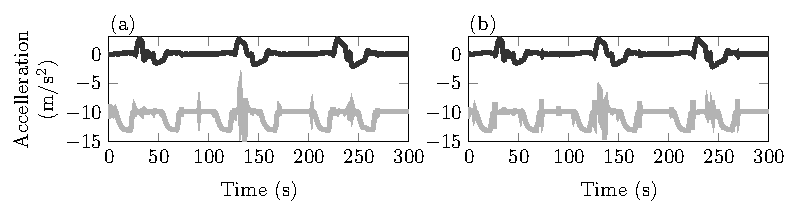
\includegraphics[]{figs/d1_patt_acc.pdf}
	\caption{Simulated vertical (\ref{line:v}) and horizontal (\ref{line:h}) accelerations on the left wing tip.}
	\label{fig:d1_patt_acc}	
\end{figure}



%%%%%%%%%%%%%%%%%%%%%%%%%%%%%%%%%%%%%%%%%%
\section{Conclusions}
In this article the design of a  flight control system for the FLEXOP flutter demonstrator, a highly flexible aircraft designed to test active flutter control algorithms, has been presented. The control system includes a baseline controller to autonomously navigate the aircraft and an active flutter control algorithm, to stabilize the unstable flutter modes and thereby extend the aircraft's operational range.
The baseline controller features a classical cascaded controller structure with various scheduled PID control loops. The flutter suppression controller is based on a novel optimal blending of the available inputs and outputs to structurally isolate the flutter modes in fictitious feedback signals. This allows designing simple SISO controllers for each of the modes, which has been carried out in detail in the paper. The controller gains for both, the baseline and the flutter suppression controller, have been selected in a model based optimization setup using robust control techniques. Two dedicated optimization setups have been proposed and solved via robust control techniques. The closed-loop has been verified using a high fidelity non-linear simulator of the test aircraft in various scenarios and results have been reported. The results show that with the developed control system it is possible to extend the aircraft's operational range beyond the open-loop flutter speed.

%%%%%%%%%%%%%%%%%%%%%%%%%%%%%%%%%%%%%%%%%%%%%%%%%%%%%%%%%%%%%%%%%%%%%%%%%%%%%%%%%%%% Helpful blocks:

%\begin{figure}[H]
%\centering
%\end{figure}   
%All figures and tables should be cited in the main text as Figure 1, Table 1, etc.

%\begin{listing}[H]
%\caption{Title of the listing}
%\rule{\textwidth}{1pt}
%\raggedright Text of the listing. In font size footnotesize, small, or normalsize. Preferred format: left aligned and single spaced. Preferred border format: top border line and bottom border line.
%\rule{\textwidth}{1pt}
%\end{listing}

%\begin{table}[H]
%	\caption{This is a table caption. Tables should be placed in the main text near to the first time they are cited.}
%	\centering
%	%% \tablesize{} %% You can specify the fontsize here, e.g.,  \tablesize{\footnotesize}. If commented out \small will be used.
%	\begin{tabular}{ccc}
%		\toprule
%		\textbf{Title 1}	& \textbf{Title 2}	& \textbf{Title 3}\\
%		\midrule
%		entry 1		& data			& data\\
%		entry 2		& data			& data\\
%		\bottomrule
%	\end{tabular}
%\end{table}

%Bulleted lists look like this:
%\begin{itemize}[leftmargin=*,labelsep=5.8mm]
%	\item	First bullet
%	\item	Second bullet
%	\item	Third bullet
%\end{itemize}
%
%Numbered lists can be added as follows:
%\begin{enumerate}[leftmargin=*,labelsep=4.9mm]
%	\item	First item 
%	\item	Second item
%	\item	Third item
%\end{enumerate}

%%%%%%%%%%%%%%%%%%%%%%%%%%%%%%%%%%%%%%%%%%%%%%%%%%%%%%%%%%%%%%%%%%%%%%%%%%%%%%%%%%%%
\vspace{6pt} 

%%%%%%%%%%%%%%%%%%%%%%%%%%%%%%%%%%%%%%%%%%%%%%%%%%%%%%%%%%%%%%%%%%%%%%%%%%%%%%%%%%%%
%% optional
%\supplementary{The following are available online at \linksupplementary{s1}, Figure S1: title, Table S1: title, Video S1: title.}

%%%%%%%%%%%%%%%%%%%%%%%%%%%%%%%%%%%%%%%%%%%%%%%%%%%%%%%%%%%%%%%%%%%%%%%%%%%%%%%%%%%%
\authorcontributions{The authors jointly developed the flight control system for the FLEXOP demonstrator and jointly wrote this article. In detail: conceptualization: D. Ossmann, M. Pusch and T. Luspay; methodology and software: M. Pusch and T. Luspay; validation: D. Ossmann and T. Luspay; writing—original draft preparation: D. Ossmann; writing—review and editing: D. Ossmann, M. Pusch and T. Luspay; visualization:   D. Ossmann and M. Pusch; supervision: D. Ossmann.}

% Example: Jean-Marc Biannic and Clément Roos jointly developed the nonlinear aircraft model and the flare control design methodology; the controller gains tuning and nonlinear simulations were initially performed by Jean-Marc Biannic and then updated by Clément Roos; Jean-Marc Biannic and Clément Roos jointly wrote the paper and its revised version.


%%%%%%%%%%%%%%%%%%%%%%%%%%%%%%%%%%%%%%%%%%%%%%%%%%%%%%%%%%%%%%%%%%%%%%%%%%%%%%%%%%%%
\funding{This work was performed in the framework of the European Union's Horizon 2020 research and innovation programme and is part of the Flutter Free FLight Envelope eXpansion for ecOnomic Performance improvement (FLEXOP) project with the  grant agreement No 636307. T. Luspay acknowledges the support by the Janos Bolyai Research Scholarship of the Hungarian Academy of Sciences.}

%%%%%%%%%%%%%%%%%%%%%%%%%%%%%%%%%%%%%%%%%%%%%%%%%%%%%%%%%%%%%%%%%%%%%%%%%%%%%%%%%%%%
%\acknowledgments{In this section you can acknowledge any support given which is not covered by the author contribution or funding sections. This may include administrative and technical support, or donations in kind (e.g., materials used for experiments).}

%%%%%%%%%%%%%%%%%%%%%%%%%%%%%%%%%%%%%%%%%%%%%%%%%%%%%%%%%%%%%%%%%%%%%%%%%%%%%%%%%%%%
\conflictsofinterest{The authors declare no conflict of interest.} 

%%%%%%%%%%%%%%%%%%%%%%%%%%%%%%%%%%%%%%%%%%%%%%%%%%%%%%%%%%%%%%%%%%%%%%%%%%%%%%%%%%%%
%%% optional
%\abbreviations{The following abbreviations are used in this manuscript:\\
%
%\noindent 
%\begin{tabular}{@{}ll}
%MDPI & Multidisciplinary Digital Publishing Institute\\
%DOAJ & Directory of open access journals\\
%TLA & Three letter acronym\\
%LD & linear dichroism
%\end{tabular}}

%%%%%%%%%%%%%%%%%%%%%%%%%%%%%%%%%%%%%%%%%%%%%%%%%%%%%%%%%%%%%%%%%%%%%%%%%%%%%%%%%%%%
%% optional
%\appendixtitles{no} %Leave argument "no" if all appendix headings stay EMPTY (then no dot is printed after "Appendix A"). If the appendix sections contain a heading then change the argument to "yes".
%\appendixsections{multiple} %Leave argument "multiple" if there are multiple sections. Then a counter is printed ("Appendix A"). If there is only one appendix section then change the argument to "one" and no counter is printed ("Appendix").
%\appendix
%\section{}
%\unskip
%\subsection{}
%The appendix is an optional section that can contain details and data supplemental to the main text. For example, explanations of experimental details that would disrupt the flow of the main text, but nonetheless remain crucial to understanding and reproducing the research shown; figures of replicates for experiments of which representative data is shown in the main text can be added here if brief, or as Supplementary data. Mathematical proofs of results not central to the paper can be added as an appendix.
%
%\section{}
%All appendix sections must be cited in the main text. In the appendixes, Figures, Tables, etc. should be labeled starting with `A', e.g., Figure A1, Figure A2, etc. 

%%%%%%%%%%%%%%%%%%%%%%%%%%%%%%%%%%%%%%%%%%
% Citations and References in Supplementary files are permitted provided that they also appear in the reference list here. 

%=====================================
% References, variant A: internal bibliography
%=====================================
\reftitle{References}
%\begin{thebibliography}{999}
%% Reference 1
%\bibitem[Author1(year)]{ref-journal}
%Author1, T. The title of the cited article. {\em Journal Abbreviation} {\bf 2008}, {\em 10}, 142-149, doi:xxxxx.
%% Reference 2
%\bibitem[Author2(year)]{ref-book}
%Author2, L. The title of the cited contribution. In {\em The Book Title}; Editor1, F., Editor2, A., Eds.; Publishing House: City, Country, 2007; pp. 32-58, ISBN.
%\end{thebibliography}


%=====================================
% References, variant B: external bibliography
%=====================================
\externalbibliography{yes}
%\bibliography{BIB_Ossmann,BIB_Ossmann-old,xBIB_Ossmann}
\bibliography{aerospace2}

%%%%%%%%%%%%%%%%%%%%%%%%%%%%%%%%%%%%%%%%%%
%% optional
%\sampleavailability{Samples of the compounds ...... are available from the authors.}

%% for journal Sci
%\reviewreports{\\
%Reviewer 1 comments and authors’ response\\
%Reviewer 2 comments and authors’ response\\
%Reviewer 3 comments and authors’ response
%}

%%%%%%%%%%%%%%%%%%%%%%%%%%%%%%%%%%%%%%%%%%
\end{document}

